%% LyX 2.3.6.1 created this file.  For more info, see http://www.lyx.org/.
%% Do not edit unless you really know what you are doing.
\documentclass[a4paper,twoside,english,ngerman,deutsch,german,sectrefs,envcountsame,envcountchap]{svmono}
\usepackage[T1]{fontenc}
\usepackage[utf8x]{inputenc}
\setcounter{tocdepth}{3}
\usepackage[pdftex]{color}
\usepackage{verbatim}
\usepackage{float}
\usepackage{units}
\usepackage{textcomp}
\usepackage{enumitem}
\usepackage{amsmath}
\usepackage{amssymb}
\usepackage{cancel}
\usepackage{makeidx}
\makeindex
\usepackage[pdftex]{graphicx}

\makeatletter

%%%%%%%%%%%%%%%%%%%%%%%%%%%%%% LyX specific LaTeX commands.
\pdfpageheight\paperheight
\pdfpagewidth\paperwidth

%% Because html converters don't know tabularnewline
\providecommand{\tabularnewline}{\\}
%% A simple dot to overcome graphicx limitations
\newcommand{\lyxdot}{.}

\floatstyle{ruled}
\newfloat{algorithm}{tbp}{loa}[chapter]
\providecommand{\algorithmname}{Algorithmus}
\floatname{algorithm}{\protect\algorithmname}

%%%%%%%%%%%%%%%%%%%%%%%%%%%%%% Textclass specific LaTeX commands.
\newlength{\lyxlabelwidth}      % auxiliary length 
\newenvironment{svmultproof}{\begin{proof}}{\qed\end{proof}}
\newenvironment{svmultproof2}{\begin{proof}}{\smartqed\qed\end{proof}}

%%%%%%%%%%%%%%%%%%%%%%%%%%%%%% User specified LaTeX commands.
%\usepackage{graphicx}
%\usepackage{color}
%\usepackage{amsmath}
\usepackage{amscd}
\usepackage{tikz-cd}
\usepackage{chapterbib}
\usepackage{makeidx}
\usepackage{multicol}
%\usepackage{footmisc}
\usepackage{cite}
\usepackage{url}
\usepackage{verbatim}
\usepackage{babelbib}
\usepackage{textgreek}
\usepackage{units}
\usepackage{listings}

% Rahmen für Maxima-Code
\usepackage[framemethod=tikz]{mdframed}
\mdfsetup{%
 outerlinewidth = 2,
 roundcorner=10pt}

% Rahmen für Maxima-Code
\newmdenv[ %
 outerlinewidth = 0.5 pt,%
 roundcorner = 5 pt,%
 backgroundcolor = gray!05,%
 innertopmargin = \topskip,%
 splittopskip = \topskip,%
]{maxima}


% Kommentare während Manuskripterstellung
% Ausgabe kann mit option "disable" ausgeschaltet werden!
%\usepackage[textsize=tiny,textwidth=30mm]{todonotes}



\newcommand{\R}{{\mathbb{R}}}
\newcommand{\C}{{\mathbb{C}}}
\newcommand{\N}{{\mathbb{N}}}
\newcommand{\Z}{{\mathbb{Z}}}
\newcommand{\V}{{\mathbb{V}}}
\newcommand{\NN}{{\mathbb{N}_0}}
\newcommand{\spann}{{\operatorname{span}}}
\newcommand{\id}{{\operatorname{id}}}
\newcommand{\im}{{\operatorname{im}}}
\newcommand{\inv}{{\operatorname{inv}}}
\newcommand{\ad}{{\operatorname{ad}}}
\newcommand{\Ad}{{\operatorname{Ad}}}
\newcommand{\adj}{{\operatorname{adj}}}
%\newcommand{\rank}{{\mathrm{rank}}}
\newcommand{\rank}{{\operatorname{rang}}}
\newcommand{\corank}{{\operatorname{corang}}}
\newcommand{\CP}{{\operatorname{cp}}}
\newcommand{\diag}{{\operatorname{diag}}}
\renewcommand{\d}{{\mathrm{d}}}
\newcommand{\e}{{\mathrm{e}}}
\newcommand{\half}{\tfrac{1}{2}}
\newcommand{\qdots}{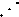
\includegraphics{qdots}}
\newcommand{\VEC}{{\mathrm{vec}\,}}
\newcommand{\hinreichend}{\glqq$\Rightarrow$\grqq}
\newcommand{\notwendig}{\glqq$\Leftarrow$\grqq}
%\renewcommand{\OE}{O.E.}
\newcommand{\partiald}[2]{\frac{\partial#1}{\partial#2}}

\renewcommand{\emph}[1]{\textbf{\em #1}}
\renewcommand{\arraystretch}{1.15}

%\providecommand{\propositionname}{Proposition}
%\newcommand{\propositionname}{Proposition}

\hyphenation{Vektor-raum Unter-vektor-raum Vektor-feld Vektor-felder
Kovektor-feld Kovektor-felder Push-forward Pull-back Teil-system}

\sloppy
\def\theoremname{Satz}
%\def\corollaryname{Folgerung}

\newtheorem{aufgabe}{Aufgabe}[chapter]
\newtheorem{loesung}{Lösung zu Aufgabe}[chapter]
 
% Umgebungsdefinition fuer Beweis
\def\halmos{\hbox{\quad\rlap{$\sqcap$}$\sqcup$}\vspace{2mm}}
 % ... aus dem Netz, ergaenzt mit qed-Zeichen (halmos)
 \newenvironment{proofsketch}[1][\textmd{\textit{Beweisskizze}}.]{\begin{trivlist}
 \item[\hskip \labelsep {\bfseries #1}]}
 {\halmos\end{trivlist}}

% für Maxima-Code
\definecolor{labelcolor}{RGB}{100,0,0}

% Minus-Zeichen als Unicode)
\DeclareUnicodeCharacter{2212}{-}


% Kommentare während Manuskripterstellung
%\newcounter{todocounter}
%\newcommand{\todonum}[2][]
%{\stepcounter{todocounter}\todo[#1]{\thetodocounter:#2}}
%\newcommand{\td}[1]{\todonum[size=\small,color=orange!50]{ #1}}

% optional
%\newcommand{\tdo}[1]{\todonum[size=\tiny,color=blue!30]{ #1}}%\todo[, #1]{#2}}

\makeatother

\usepackage{babel}
\addto\captionsenglish{\renewcommand{\algorithmname}{Algorithm}}
\addto\captionsenglish{\renewcommand{\corollaryname}{Corollary}}
\addto\captionsenglish{\renewcommand{\definitionname}{Definition}}
\addto\captionsenglish{\renewcommand{\examplename}{Example}}
\addto\captionsenglish{\renewcommand{\lemmaname}{Lemma}}
\addto\captionsenglish{\renewcommand{\proofname}{Proof}}
\addto\captionsenglish{\renewcommand{\propositionname}{Proposition}}
\addto\captionsenglish{\renewcommand{\remarkname}{Remark}}
\addto\captionsenglish{\renewcommand{\theoremname}{Theorem}}
\addto\captionsngerman{\renewcommand{\algorithmname}{Algorithmus}}
\addto\captionsngerman{\renewcommand{\corollaryname}{Korollar}}
\addto\captionsngerman{\renewcommand{\definitionname}{Definition}}
\addto\captionsngerman{\renewcommand{\examplename}{Beispiel}}
\addto\captionsngerman{\renewcommand{\lemmaname}{Lemma}}
\addto\captionsngerman{\renewcommand{\proofname}{Beweis}}
\addto\captionsngerman{\renewcommand{\propositionname}{Satz}}
\addto\captionsngerman{\renewcommand{\remarkname}{Bemerkung}}
\addto\captionsngerman{\renewcommand{\theoremname}{Theorem}}
\providecommand{\corollaryname}{Korollar}
\providecommand{\definitionname}{Definition}
\providecommand{\examplename}{Beispiel}
\providecommand{\lemmaname}{Lemma}
\providecommand{\proofname}{Beweis}
\providecommand{\propositionname}{Satz}
\providecommand{\remarkname}{Bemerkung}
\providecommand{\theoremname}{Theorem}

\begin{document}

\frontmatter{}
\title{Nichtlineare Regelungssysteme}
\subtitle{Theorie und Anwendung der exakten Linearisierung}
\author{Klaus Röbenack}

\maketitle

\preface{}

Nichtlineare Regelungs- und Steuerungsverfahren kommen überall dort
zum Einsatz, wo die Leistungsfähigkeit linearer Methoden an ihre Grenzen
stößt. An- und Abfahrvorgänge bzw. Arbeitspunktwechsel in chemischen
Reaktoren, die hochpräzise Lageregelung von Starrkörpern im Raum (beispielsweise
Effektoren von Industrierobotern oder autonome Flugkörper) oder die
Regelung leistungselektronischer Baugruppen mögen als Beispiele dienen.
Vor diesem Hintergrund verwundert es nicht, dass Ansätze zur nichtlinearen
Regelung in der industriellen Praxis zunehmend auf Interesse stoßen,
um die Ausbeute und Zuverlässigkeit der zugrundliegenden technischen
Prozesse zu erhöhen. Gleichwohl ist der in der nichtlinearen Regelungstheorie
verwendete mathematische Apparat gefürchtet. Genau an dieser Stelle
setzt dieses Lehrbuch an: Die Darstellung ist einerseits in sich mathematisch
schlüssig und nachvollziehbar, andererseits aber auch in einer für
Ingenieure verständlichen Sprache formuliert. Der inhaltliche Fokus
des Buches liegt dabei auf der Methode der exakten Linearisierung
zum Regler- und Beobachterentwurf.

Das Buch richtet sich maßgeblich an Studierende der Elektrotechnik
und Mechatronik in der Vertiefungsrichtung Automatisierungs- bzw.
Regelungstechnik, die bereits über fortgeschrittene regelungstechnische
Kenntnisse verfügen. Doktoranden können anhand des Buches ihr systemtheoretisches
bzw. regelungstechnisches Verständnis nichtlinearer Systeme vertiefen.
Für Ingenieure in der Industrie, die mit der Regelung nichtlinearer
Systeme konfrontiert sind, werden verschiedene Entwurfsansätze detailliert
beschrieben.

Im Teil~\ref{part:Vorbereitung} des Buches werden nach einigen Einführungsbeispielen
die benötigten mathematischen Konzepte aus den Bereichen der linearen
Algebra, der Vektoranalysis bzw. der Differentialgeometrie vermittelt.
Zur Festigung der Lehrinhalte sind am Ende der Kapitel~\ref{cha:Grundlagen}
und~\ref{chap:Diff-Geo} Übungsaufgaben vorgesehen. Die Teile~\ref{part:Reglerentwurf}
und~\ref{part:Beobachterentwurf} behandeln den Regler- bzw. Beobachterentwurf.
Die jeweilige Herangehensweise bzw. Entwurfsmethodik wird an verschiedenen
Beispielen veranschaulicht bzw. durch den Einsatz des Open-Source-Computeralgebrasystems
\textsc{Maxima} illustriert.

Erste Skizzen zum vorliegenden Buch entstanden in Verbindung mit der
Vorlesung ,,Mathematische Grundlagen der nichtlinearen Regelungstheorie``,
die ich im Sommersemester 2006 an der Fakultät Mathematik und Naturwissenschaften
der TU Dresden hielt. Diese Lehrveranstaltung führe ich seit 2007
als Wahlpflichtfach ,,Nichtlineare Regelungstechnik 2`` für verschiedene
Ingenieurstudiengänge fort. Meine zehnjährige Lehrtätigkeit in diesem
Gebiet hat das vorliegende Buch maßgeblich geprägt.

Es ist mir ein Bedürfnis, zuallererst meinem Lehrer, Herrn Prof. Kurt
Reinschke, für seine langjährige Unterstützung zu danken. Besonderer
Dank gilt auch Herrn Prof. Andreas Griewank für seine Anregungen zur
Beschäftigung mit dem algorithmischen Differenzieren. Ebenso möchte
ich Herrn Prof. Wolfgang V. Walter danken, durch den ich in den Jahren
2006 bis 2007 die Vertretung der Professur ,,Wissenschaftliches Rechnen
und Angewandte Mathematik`` wahrnehmen konnte.

Bei der Gestaltung der dem Buch zugrundeliegenden Vorlesung und der
Konzeption des Manuskripts haben mich zahlreiche Diplomanden, heutige
und ehemalige Mitarbeiter und Doktoranden unterstützt. Besonderer
Dank gilt Dr. Carsten Knoll, der das Buch durch zahlreiche Verbesserungsvorschläge
erheblich bereichert hat. Außerdem danke ich Dr. Jan Winkler, Dr.
Matthias Franke und Prof. Frank Woittennek für die angenehme Zusammenarbeit
und die interessanten Diskussionen. Herrn M.Sc. Rick Voßwinkel danke
ich für die sehr gewissenhafte Durchsicht des Manuskripts. Mein Dank
gebührt auch Dr. Carsten Collon, Dipl.-Ing. Mirko Franke, Dipl.-Ing.
Chenzi Huang, Dipl.-Ing. Fabian Paschke, Dipl.-Ing. Klemens Fritzsche,
Dipl.-Ing. Gunter Nitzsche und Dipl.-Ing. Robert Huber.

Zahlreiche Diskussionen bei Konferenzen, Tagungen und Workshops haben
mein Verständnis für nichtlineare Systeme vertieft. Für fachliche
Anregungen möchte ich daher Dr. Albrecht Gensior (TU Dresden), Associate
Prof. Pranay Goel (Indian Institute of Science Education and Research,
Pune), PD Dr. Lutz Gröll (Karlsruher Institut für Technologie), Prof.
Alan F. Lynch (University of Alberta, Kanada), Prof. Jaime A. Moreno
(Universidad Nacional Autónoma de México), Prof. Joachim Rudolph (Universität
des Saarlandes), Prof. Andrea Walther (Universität Paderborn) und
Prof. Zeitz (Universität Stuttgart) danken.

Frau Eva Hestermann-Beyerle und Frau Birgit Kollmar-Thoni vom Springer-Verlag
danke ich für die angenehme Zusammenarbeit. Mein Dank gilt auch dem
\hbox{De~Gruyter}-Verlag für die Nutzungsgenehmigung im Zusammenhang
mit Kapitel~\ref{cha:Beobachter-Normalform}. Meiner Frau und meinen
Kindern danke ich für ihre Geduld und ihr Verständnis.

\vspace{\baselineskip}

\noindent \begin{flushright}
Dresden, März 2017\hfill{}Klaus Röbenack
\par\end{flushright}


\mainmatter{}

\tableofcontents{}
\part{Vorbereitung\label{part:Vorbereitung}}

\chapter{Motivationsbeispiele\label{chap:Einleitung}}

Dieses Kapitel befasst sich mit der Modellierung einiger technischer
Beispielsysteme, bei denen man auf nichtlineare Modellgleichungen
geführt wird. Auf diese Beispielsysteme wird in den weiteren Kapiteln
mehrfach zurückgegriffen.

\section{Mobiler Roboter\label{subsec:Mobiler-Roboter-Modellierung}}

Mobile Roboter spielen eine wichtige Rolle bei der automatisierten
Lagerhaltung und bei flexiblen Fertigungsprozessen, finden aber auch
als Inspektions- bzw. Serviceroboter Anwendung. Abb.~\ref{fig:mobiler-roboter-kinematisches-modell}~(links)
stellt einen für Lehrzwecke entwickelten mobilen Roboter mit zwei
Rädern dar~\cite{roebenack2015roboter}.

\begin{figure}
\begin{centering}
\begin{tabular}{ccc}
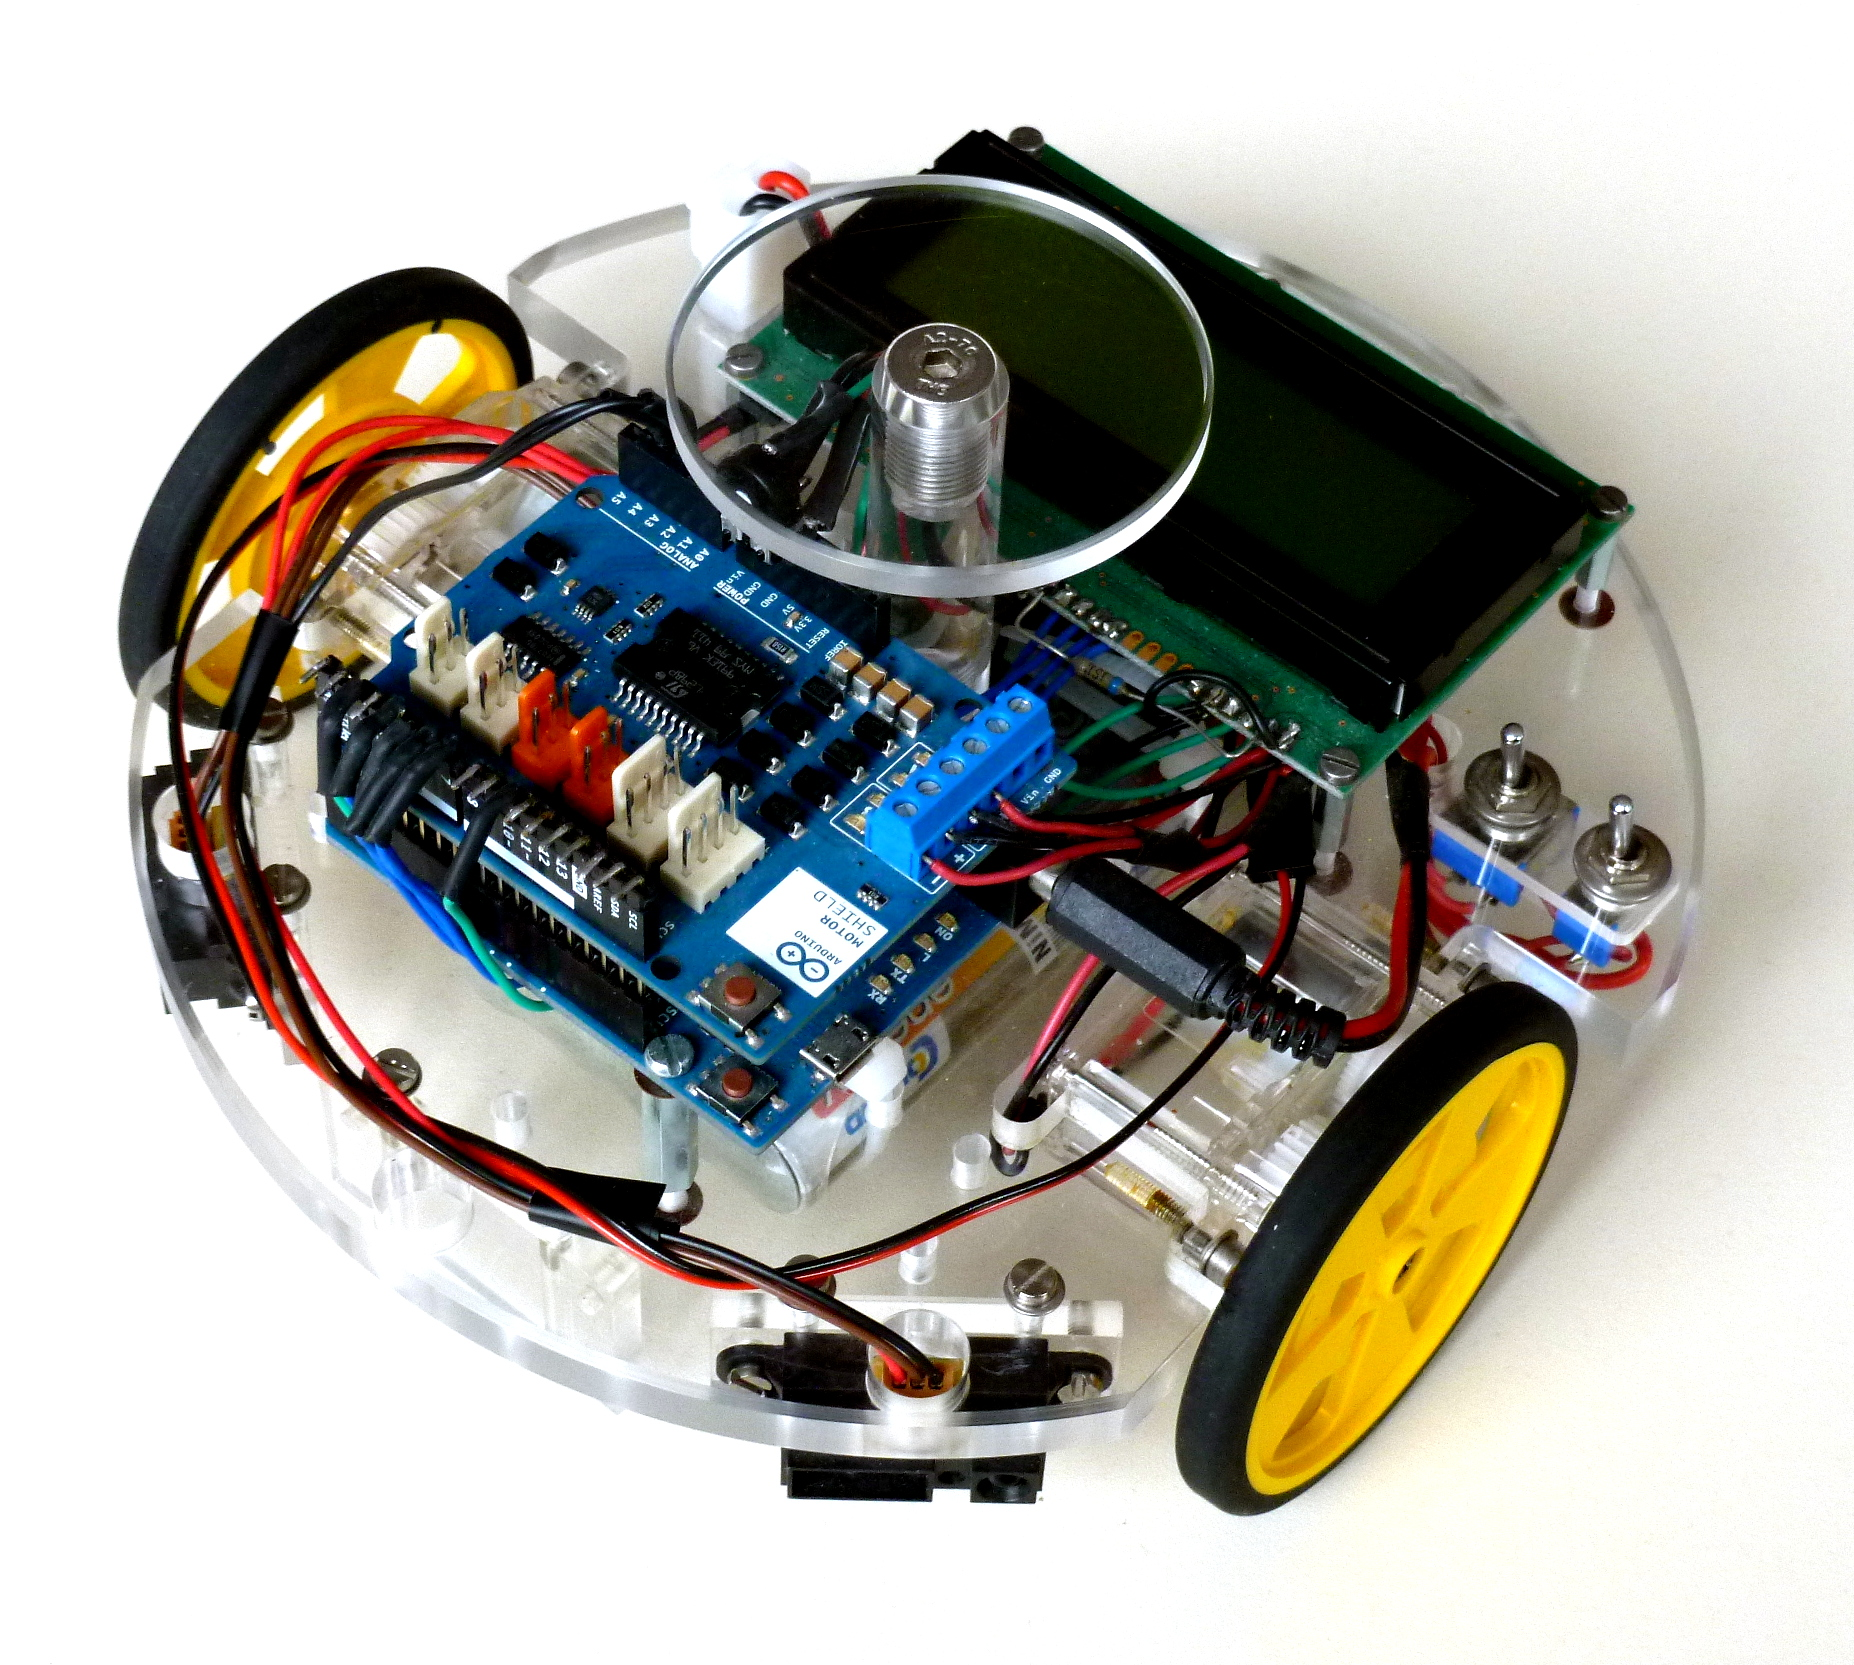
\includegraphics[width=0.45\textwidth]{Roboter_Foto} & \hspace*{0.05\textwidth} & 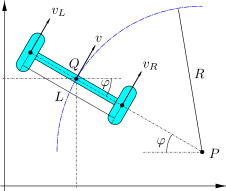
\includegraphics[width=0.45\textwidth]{Roboter_kin_Modell}\tabularnewline
\end{tabular}
\par\end{centering}
\caption{Mobiler Roboter, Prototyp nach~\cite{roebenack2015roboter} (links),
Modell in der $(x_{1},x_{2})$-Ebene (rechts)\label{fig:mobiler-roboter-kinematisches-modell}}
\end{figure}

Für den mobilen Roboters wird nachfolgend ein kinematisches Modell
hergeleitet. Dieses Modell beschreibt die Bewegung in der Ebene ohne
Berücksichtigung der die Bewegung verursachenden Kräfte. Der Antrieb
des Roboters erfolgt über zwei Räder mit dem Radius~$r$. Das linke
Rad habe die Winkelgeschwindigkeit $\omega_{L}$, das rechte die Winkelgeschwindigkeit
$\omega_{R}$. An den Auflagepunkten der Räder erhält man die Tangentialgeschwindigkeiten
\[
\begin{array}{lcl}
v_{L} & = & \omega_{L}r,\\
v_{R} & = & \omega_{R}r.
\end{array}
\]
Für unterschiedliche Winkelgeschwindigkeiten (also $\omega_{L}\neq\omega_{R}$)
dreht sich der Roboter. Wir stellen uns diese Drehung als Umfahrung
eines (fiktiven) Punktes~$P$ vor, der zum Mittelpunkt~$Q$ des
Roboters den Abstand~$R$ habe. Linkes und rechtes Rad haben von
dem Punkt~$P$ die Abstände
\[
\begin{array}{lcl}
R_{L} & = & R+\frac{L}{2},\\
R_{R} & = & R-\frac{L}{2},
\end{array}
\]
wobei~$L$ den Abstand beider Räder voneinander bezeichnet. Beschreibt
man die Rotation um den Punkt~$P$ mit dem in Abb.~\ref{fig:mobiler-roboter-kinematisches-modell}~(rechts)
eingeführten Winkel~$\varphi$, so erhält man die Rotationgeschwindigkeit
\begin{equation}
\omega=\dot{\varphi}\label{eq:roboter-modell-rot}
\end{equation}
als zeitliche Ableitung des Winkels. Zu den Tangentialgeschwindigkeiten
der beiden Räder besteht dann der Zusammenhang
\[
\begin{array}{lcl}
v_{L} & = & \omega R_{L},\\
v_{R} & = & \omega R_{R}.
\end{array}
\]
Aus gegebenen Winkelgeschwindigkeiten~$\omega_{L}$ und~$\omega_{R}$
der Motoren kann man damit einerseits die Rotationsgeschwindigkeit
des Roboters um die eigene Achse bestimmen
\[
\omega=\frac{r}{L}\left(\omega_{L}-\omega_{R}\right),
\]
andererseits auch den Abstand
\[
R=\frac{L}{2}\left(\frac{\omega_{L}+\omega_{R}}{\omega_{L}-\omega_{R}}\right)
\]
zwischen dem Punkt~$Q$ und dem Drehpunkt~$P$. Damit erhält man
zugleich die translatorische Geschwindigkeit 
\[
v=\omega R=\frac{r}{2}\left(\omega_{L}+\omega_{R}\right)
\]
des Roboters. Mit dem Winkel~$\varphi$ und der Geschwindigkeit~$v$
lässt sich die translatorische Bewegung beschreiben: 
\begin{equation}
\begin{array}{lcl}
\dot{x}_{1} & = & v\,\sin\varphi,\\
\dot{x}_{2} & = & v\,\cos\varphi.
\end{array}\label{eq:roboter-modell-trans}
\end{equation}
Führt man den Zustand 
\[
x=\left(\begin{array}{c}
x_{1}\\
x_{2}\\
x_{3}
\end{array}\right)=\left(\begin{array}{c}
x_{1}\\
x_{2}\\
\varphi
\end{array}\right)
\]
sowie die Eingänge $u_{1}=v$ und $u_{2}=\omega$ ein, so liefert
die Kombination aus~(\ref{eq:roboter-modell-rot}) und~(\ref{eq:roboter-modell-trans})
das kinematische Gesamtmodell 
\begin{equation}
\left(\begin{array}{c}
\dot{x}_{1}\\
\dot{x}_{2}\\
\dot{x}_{3}
\end{array}\right)=\left(\begin{array}{c}
\sin x_{3}\\
\cos x_{3}\\
0
\end{array}\right)u_{1}+\left(\begin{array}{c}
0\\
0\\
1
\end{array}\right)u_{2}.\label{eq:roboter-kinematisches-modell}
\end{equation}
Bedingt durch die Winkelfunktionen liegt damit ein Modell als nichtlineares
Differentialgleichungssystem vor. Genauer gesagt ist das Modell~(\ref{eq:roboter-kinematisches-modell})
nichtlinear bezüglich des Zustands~$x$, aber linear hinsichtlich
der Eingänge~$u_{1}$ und~$u_{2}$.

Das kinematische Robotermodell~(\ref{eq:roboter-kinematisches-modell})
lässt sich als einachsiges Fahrzeugmodell aufgefassen. Kinematische
Fahrzeugmodelle werden auch bei aktuellen Forschungsvorhaben genutzt,
beispielsweise bei der Spurregelung und beobachterbasierten Spurschätzung
für mehrachsige, mehrgliedrige bzw. mehr\-achs\-gelenkte Fahrzeuge
(LKWs, LKWs mit Anhänger, überlange Beförderungssysteme wie z.\,B.
AutoTram\textsuperscript{\textregistered}, siehe \cite{huber2012ssd,nitzsche2014ecc,riesmeier2016}).

\section{Wagen mit Pendel\label{subsec:Wagen-mit-Pendel}}

Verladebrücken bzw. Brückenkräne werden in Montagehallen, in Lagern
und auf Güterumschlagplätzen (z.\,B. Güterbahnhöfen, Häfen) eingesetzt.
Für eine schnelle Bewegung bzw. hochpräzise Positionierung der zu
transportierenden Lasten ist eine Regelung erforderlich.

Aus physikalischer Sicht kann man eine Verladebrücke als ein horizontal
bewegliches Pendel auffassen. Abb.~\ref{fig:Wagen-mit-Pendel} zeigt
einen Wagen, an welchem ein Pendel der Länge~$\ell$ angebracht ist.
Zur Vereinfachung gehen wir von einer festen Seillänge~$\ell$ aus.
Der Wagen habe die Masse~$m_{1}$, die Last die Masse~$m_{2}$.
Das Seil selber werde als masselos angenommen. Die Lage des Systems
wird durch die Wagenposition~$q_{1}$ und den Pendelwinkel~$q_{2}$
beschrieben. Eine auf den Wagen wirkende Kraft~$\digamma$ stellt
den Eingang des Wagen-Pendel-Systems dar.

\begin{figure}
\begin{centering}
\resizebox{0.5\textwidth}{!}{\input{wagen_pendel.pdftex_t}}
\par\end{centering}
\caption{Wagen mit Pendel\label{fig:Wagen-mit-Pendel}}

\end{figure}

Die kinetische Energie hat die Form
\[
T=\frac{m_{1}}{2}\dot{q}_{1}^{2}+\frac{m_{2}}{2}\left(\dot{x}_{s}^{2}+\dot{y}_{s}^{2}\right),
\]
wobei die Position der Last durch die Koordinaten 
\begin{eqnarray*}
x_{s} & = & q_{1}+\ell\sin q_{2}\\
y_{s} & = & \ell\cos q_{2}
\end{eqnarray*}
beschrieben wird. Daraus ergibt sich unmittelbar 
\[
T=\frac{m_{1}+m_{2}}{2}\dot{q}_{1}^{2}+m_{2}\ell\dot{q}_{1}\dot{q}_{2}\cos q_{2}+\frac{m_{2}}{2}\ell^{2}\dot{q}_{2}^{2}.
\]
Mit der potentiellen Energie 
\[
V=m_{2}g\ell(1-\cos q_{2})
\]
erhält man die Lagrange-Funktion $L=T-V$. Die Bewegungsgleichungen
haben die Form
\[
M(q)\ddot{q}+C(q,\dot{q})+K(q)=Q
\]
mit der Massematrix 
\[
M(q)=\left(\begin{array}{cc}
m_{1}+m_{2} & \ell m_{2}\cos q_{2}\\
\ell m_{2}\cos q_{2} & \ell^{2}m_{2}
\end{array}\right).
\]
Die Vektoren~$C$ und~$K$ beinhalten die Zentrifugal- und Corioliskräfte
bzw. die Potentialkräfte 
\[
C(q,\dot{q})=\left(\begin{array}{c}
-\ell m_{2}\dot{q}_{2}^{2}\sin q_{2}\\
\text{0}
\end{array}\right),\quad K(q)=\left(\begin{array}{c}
0\\
m_{2}g\ell\sin q_{2}
\end{array}\right).
\]
Als äußere Kräfte wirken die Reibungskräfte (viskose Reibung mit den
Koeffizienten~$d_{1}$ und~$d_{2}$) sowie die auf den Wagen eingeprägte
Kraft~$\digamma$:
\[
Q=\left(\begin{array}{c}
\digamma-d_{1}\dot{q}_{1}\\
-d_{2}\dot{q}_{2}
\end{array}\right).
\]
Mit dem Zustand $x=(q_{1},\dot{q}_{1},q_{2},\dot{q}_{2})^{T}$ und
dem Eingang $u=\digamma$ erhält man das folgende nichtlineare Modell:
\begin{equation}
\begin{array}{lcl}
\dot{x}_{1} & = & x_{2}\\
\dot{x}_{2} & = & \frac{m_{2}\ell^{2}x_{4}^{2}\sin x_{3}-d_{1}\ell x_{2}+\cos x_{3}\left(m_{2}g\ell\sin x_{3}+d_{2}x_{4}\right)+\ell u}{\ell\left(m_{1}+m_{2}\sin^{2}x_{3}\right)}\\
\dot{x}_{3} & = & x_{4}\\
\dot{x}_{4} & = & \frac{-\left(m_{1}+m_{2}\right)\left(m_{2}g\ell\sin x_{3}+d_{2}x_{4}\right)-\cos x_{3}\left(\ell^{2}m_{2}^{2}x_{4}^{2}\sin x_{3}-d_{1}\ell m_{2}x_{2}\right)-\ell m_{2}u\cos x_{3}}{\ell^{2}m_{2}\left(m_{1}+m_{2}\sin^{2}x_{3}\right)}
\end{array}\label{eq:modell-pendel-mit-wagen}
\end{equation}
Das Modell ist nichtlinear im Zustand~$x$, aber affin im Eingang~$u$.

\section{Hochsetzsteller\label{subsec:Hochsetzsteller-Modellierung}}

Mit Spannungswandlern lassen sich verschiedene Spannungsniveaus aneinander
anpassen, z.\,B. zwischen einer bereitgestellten Versorgungsspannung
und einem Verbraucher. Gleichsspannungswandler sind ein beliebte Objekte
für die Erprobung und den Vergleich nichtlinearer Regelungsverfahren~\cite{sira-ramirez1991ijc,kugi2000at,gensior2006}.
Aufgrund ihres Wirkungsgrades werden geschaltete Spannungswandler
in vielen Bereichen der Leistungselektronik und der Antriebstechnik
eingesetzt.

Ein \emph{Hochsetzsteller}\index{Hochsetzsteller} bzw. \emph{Aufwärtswandler}
(engl. \emph{Boost Converter}) ist ein Gleichspannungswandler, der
eine Eingangsspannung in eine höhere Ausgangsspannung überführt~\cite{erickson2004,bacha2014}.
Das Schaltbild in Abb.~\ref{fig:hochsetzsteller-schaltbild-netzwerk}
zeigt die grundsätzliche Schaltungstopologie bzw. das Netzwerkmodell
eines Hochsetzstellers. Der Leistungstransistor wird zusammen mit
der Freilaufdiode als Umschalter modelliert, wobei $d=1$ einem durchgesteuerten
Transistor und $d=0$ einem sperrenden Transistor entspricht. 

\begin{figure}
\begin{centering}
\resizebox{0.99\textwidth}{!}{\input{schaltbild-boost-konverter.pdftex_t}}
\par\end{centering}
\caption{Prinzipschaltbild (links) und Netzwerkmodell (rechts) eines Hochsetzstellers\label{fig:hochsetzsteller-schaltbild-netzwerk}}

\end{figure}
Für den Spulenstrom~$I$ gilt aufgrund des Maschensatzes 
\[
L\dot{I}=E+\left\{ \begin{array}{rcl}
0 & \text{für} & d=1,\\
-U & \text{für} & d=0.
\end{array}\right.
\]
Die Bilanzierung der in den Kondensator fließenden Ströme (Knotensatz)
liefert 
\[
C\dot{U}=-\frac{U}{R}+\left\{ \begin{array}{rcl}
0 & \text{für} & d=1,\\
I & \text{für} & d=0.
\end{array}\right.
\]
Mit Einführung des Vektors $x=(x_{1},x_{2})^{T}=(I,U)^{T}$ erhält
man das Differentialgleichungssystem 
\begin{equation}
\begin{array}{lcl}
\dot{x}_{1} & = & -(1-d)\frac{1}{L}x_{2}+\frac{E}{L},\\
\dot{x}_{2} & = & (1-d)\frac{1}{C}x_{1}-\frac{1}{RC}x_{2}.
\end{array}\label{eq:Hochsetzsteller-modell}
\end{equation}
Das System ist aufgrund der Produktbildung zwischen dem Eingang~$d$
und den Komponenten des Zustands~$x$ nichtlinear. Ein solches Modell
nennt man auch bilinear~\cite{schwarz91}.

Der Eingang~$d$ beschreibt das Verhalten des als Schalter modellierten
Transistors und kann zunächst nur die diskreten Werte $d\in\{0,1\}$
annehmen. In diesem Kontext liegt mit Gl.~(\ref{eq:Hochsetzsteller-modell})
ein \emph{geschaltetes Modell} (engl. \emph{switched model}) vor.
Mit einer \emph{Pulsweitenmodulation} (kurz \emph{PWM}, engl. \emph{pulse
width modulation}) lassen sich auch Zwischenwerte einstellen (siehe
Abb.~\ref{fig:PWM}). Das Verhältnis der Einschaltzeit mit $d=1$
gegenüber der Schaltperiode $T>0$ bezeichnet man dabei als as \emph{Tastverhältnis~}$\bar{d}$
(engl. \emph{duty ratio}), welches Werte aus dem Intervall $\bar{d}\in[0,1]$
annehmen kann.

\begin{figure}
\begin{centering}
\resizebox{0.55\textwidth}{!}{\input{PWM.pdftex_t}}
\par\end{centering}
\caption{Signalverlauf des Eingangs~$d$ bei Pulsweitenmodulation (PWM)\label{fig:PWM}}
\end{figure}

Das Tastverhältnis~$\bar{d}$ gibt den Mittelwert des Schaltsignals~$d$
über eine Periode~$T$ an:
\[
\bar{d}(t)=\frac{1}{T}\int_{t}^{t+T}d(\tau)\,\d\tau.
\]
In analoger Weise kann man auch für alle anderen Systemgrößen (Ströme,
Spannungen, ggf. Ladungen usw.) gemittelte Größen einführen. In diesem
Sinne erhält man mit 
\[
\bar{x}_{i}(t)=\frac{1}{T}\int_{t}^{t+T}x_{i}(\tau)\,\d\tau\quad\text{für}\quad i=1,2
\]
die gemittelten Zustandskomponenten aus dem Modell~(\ref{eq:Hochsetzsteller-modell}).
Der zeitliche Verlauf der gemittelten Größen lässt sich wiederum durch
ein Differentialgleichungssystem beschreiben. Für den Grenzübergang
$T\to0$, was aus technischer Sicht durch eine hinreichend hohe Schaltfrequenz
$1/T$ angenähert wird, erhält man für die gemittelten Größen das
\emph{gemittelte Modell} (engl. \emph{averaged model}):
\begin{equation}
\begin{array}{lcl}
\dot{\bar{x}}_{1} & = & -(1-\bar{d})\frac{1}{L}\bar{x}_{2}+\frac{E}{L}\\
\dot{\bar{x}}_{2} & = & (1-\bar{d})\frac{1}{C}\bar{x}_{1}-\frac{1}{RC}\bar{x}_{2}.
\end{array}\label{eq:Hochsetzsteller-modell-gemittelt}
\end{equation}
Das gemittelte Modell~(\ref{eq:Hochsetzsteller-modell-gemittelt})
in seiner Struktur vollständig mit dem Modell~(\ref{eq:Hochsetzsteller-modell})
übereinstimmt, wird man in der praktischen Handhabung darauf verzichten,
die gemittelen Größen separat auszuweisen. Den Reglerentwurf führt
man an dem (hinsichtlich des Eingangssignals wertkontunierlichen)
gemittelten Modell durch, bei der Implementierung wird das Reglerausgangssignal
nach einer Pulsweitenmodulation dem geschalteten System zugeführt.

\bibliographystyle{babalpha}
\bibliography{dynamic}



%% LyX 2.3.6.1 created this file.  For more info, see http://www.lyx.org/.
%% Do not edit unless you really know what you are doing.
\documentclass[a4paper,ngerman,german,deutsch,sectrefs]{svmono}
\usepackage[T1]{fontenc}
\usepackage[utf8]{inputenc}
\setcounter{tocdepth}{3}
\usepackage{color}
\usepackage{amsmath}
\usepackage{amssymb}
\usepackage{graphicx}

\makeatletter

%%%%%%%%%%%%%%%%%%%%%%%%%%%%%% LyX specific LaTeX commands.
\pdfpageheight\paperheight
\pdfpagewidth\paperwidth

%% A simple dot to overcome graphicx limitations
\newcommand{.}{.}


%%%%%%%%%%%%%%%%%%%%%%%%%%%%%% Textclass specific LaTeX commands.
\newenvironment{svmultproof}{\begin{proof}}{\qed\end{proof}}

\makeatother

\usepackage{babel}
\providecommand{\corollaryname}{Korollar}
\providecommand{\examplename}{Beispiel}
\providecommand{\lemmaname}{Lemma}
\providecommand{\proofname}{Beweis}
\providecommand{\propositionname}{Satz}
\providecommand{\remarkname}{Bemerkung}
\providecommand{\theoremname}{Theorem}

\begin{document}

\chapter{Mathematische Grundlagen\label{cha:Grundlagen}}
$\frac{\partial^{}L_{\f}^k h(\x)}{\partial{x}^{}}$
Dieser Abschnitt soll dem Leser einige Grundlagen der linearen Abgebra
sowie der Vektoranalysis in Erinnerung rufen. Dabei finden auch erste
Begriffe und Konzepte der Differentialgeometrie Erwähnung. Zusätzlich
werden ausgewählte Aspekte gewöhnlicher Differentialgleichungssysteme
behandelt. In diesem Kapitel werden nur diejenigen Aussagen bewiesen,
die für regelungstheoretische Anwendungen in den folgenden Abschnitten
des Buches von besonderer Bedeutung sind. Zur Festigung und Vertiefung
der behandelten Konzepte seien dem Leser die Lehrbücher~\cite{arnold2001,kerner2007}
empfohlen.

\section{Lineare Algebra\label{sec:Lineare-Algebra}}

Sei ${\mathbb{R}}$ die Menge der reellen Zahlen. Der $n$-dimensionale reelle
Vektorraum wird mit ${\mathbb{R}}^{n}$ bezeichnet, seine Elemente heißen \textbf{\em Vektoren}.
Ein Vektor $x\in{\mathbb{R}}^{n}$ wird oft in der Form eines Spaltenvektors
\begin{equation}
x=\left(\begin{array}{c}
x_{1}\\
\vdots\\
x_{n}
\end{array}\right)\label{eq:vektor-x}
\end{equation}
mit den Komponenten $x_{1},\ldots,x_{n}\in{\mathbb{R}}$ dargestellt. Zur Unterscheidung
von Zeilenvektoren spricht man hier auch von \textbf{\em kontravarianten
Vektoren}.

Die $n$ Einheitsvektoren
\[
e_{1}=\left(\begin{array}{c}
1\\
0\\
\vdots\\
0
\end{array}\right),\ldots,e_{n}=\left(\begin{array}{c}
0\\
\vdots\\
0\\
1
\end{array}\right)
\]
bilden eine Basis des~${\mathbb{R}}^{n}$, die sogenannte \textbf{\em kanonische
Basis} oder \textbf{\em Standardbasis}. Jeder Vektor~(\ref{eq:vektor-x})
lässt sich eindeutig als Linearkombination der Basisvektoren darstellen:
\[
x=x_{1}e_{1}+\cdots+x_{n}e_{n}.
\]
Die \textbf{\em lineare Hülle} (engl. \textbf{\em linear
hull, linear span}) von $r$ Vektoren $v_{1},\ldots,v_{r}\in{\mathbb{R}}^{n}$
ist die Menge aller Linearkombinationen dieser Vektoren:
\[
{\operatorname{span}}\left\{ v_{1},\ldots,v_{r}\right\} :=\left\{ \alpha_{1}v_{1}+\cdots+\alpha_{r}v_{r};\,\alpha_{1},\ldots,\alpha_{r}\in{\mathbb{R}}\right\} .
\]
Die lineare Hülle ist damit ein \textbf{\em Untervektorraum}, \textbf{\em Unterraum}
bzw. \textbf{\em Teilraum} (engl. \textbf{\em subspace}) des~${\mathbb{R}}^{n}$, d.\,h.
eine nichtleere Teilmenge des~${\mathbb{R}}^{n}$, welche selber ein Vektorraum
ist.

Zu zwei Vektoren $x,y\in{\mathbb{R}}^{n}$ definiert man durch
\begin{equation}
(x,y):=\sum_{i=1}^{n}x_{i}y_{i}\label{eq:skalarprodukt}
\end{equation}
das (\textbf{\em kanonische}) \textbf{\em Skalarprodukt}.
Die Vektoren~$x$ und~$y$ sind zueinander \textbf{\em orthogonal} (bzw.
stehen \textbf{\em senkrecht aufeinander}), falls
\[
(x,y)=0.
\]

Jeder Unterraum~$\mathbb{U}$ des ${\mathbb{R}}^{n}$ kann mit Hilfe eines
geeignet gewählten weiteren Unterraums~$\mathbb{V}$ zum ursprünglichen
Vektorraum~${\mathbb{R}}^{n}$ ergänzt werden, so dass
\[
{\mathbb{R}}^{n}=\mathbb{U}+\mathbb{V}.
\]
Haben zusätzlich beide Unterräume nur den Nullvektor gemeinsam, d.\,h.
\[
\mathbb{U}\cap\mathbb{V}=\{0\},
\]
dann ist der Unterraum~$\mathbb{V}$ der \textbf{\em Komplementärraum}
(bzw. das \textbf{\em Komplement}) des Unterraumes~$\mathbb{U}$. In diesem
Fall kann man den Vektorraum~${\mathbb{R}}^{n}$ als \textbf{\em direkte Summe} der
beiden Unterräume darstellen:
\[
{\mathbb{R}}^{n}=\mathbb{U}\oplus\mathbb{V}.
\]
Die Zerlegung in direkte Summen bedeutet, dass es für jeden Vektor
$x\in{\mathbb{R}}^{n}$ eine eindeutige Darstellung $x=u+v$ mit $u\in\mathbb{U}$
und $v\in\mathbb{V}$ gibt.

Die Ergänzung eines Unterraumes~$\mathbb{U}$ um einen Komplmentärraum~$\mathbb{V}$
ist nicht eindeutig. Wählt man den Komplementärraum unter Zuhilfenahme
des Skalarprodukts~(\ref{eq:skalarprodukt}) derart, dass alle Vektoren
$u\in\mathbb{U}$ und $v\in\mathbb{V}$ jeweils senkrecht aufeinander
stehen, so erhält man das \textbf{\em orthogonale Komplement}~$\mathbb{U}^{\perp}$
von~$\mathbb{U}$:
\begin{equation}
\mathbb{U}^{\perp}:=\{v\in{\mathbb{R}}^{n};\;\forall u\in\mathbb{U}:\,(u,v)=0\}.\label{eq:ortho-komplement}
\end{equation}
Hinsichtlich der Dimensionen besteht folgender Zusammenhang (\textbf{\em Dimensionsformel}):
\begin{equation}
\dim\mathbb{U}+\dim\mathbb{U}^{\perp}=n.\label{eq:dimensionsformel-ortho-kompl}
\end{equation}

\begin{example}
\label{exa:orthogonales-Komplement}Die Vektoren
\[
u_{1}=\left(\begin{array}{c}
1\\
2\\
3
\end{array}\right)\quad\text{und}\quad u_{2}=\left(\begin{array}{c}
4\\
5\\
6
\end{array}\right)
\]
spannen im Vektorraum ${\mathbb{R}}^{3}$ einen zweidimensionalen Unterraum
$\mathbb{U}={\operatorname{span}}\{u_{1},u_{2}\}$ auf. In \textsc{Maxima}~\cite{maxima,haager2014}
definiert man die Spaltenvektoren mit dem Befehl \texttt{columnvector}
aus dem Paket \texttt{eigen}. Das orthogonale Komplement ist eindimensional
und wird von dem Vektor
\[
v=\left(\begin{array}{c}
-3\\
6\\
-3
\end{array}\right)
\]
aufgespannt:


\end{example}

Eine $m\times n$-Matrix $A\in{\mathbb{R}}^{m\times n}$ besteht aus $m$ Zeilen
und $n$ Spalten:
\[
A=\left(\begin{array}{ccc}
a_{11} & \cdots & a_{1n}\\
\vdots & \ddots & \vdots\\
a_{m1} & \cdots & a_{mn}
\end{array}\right).
\]
Gilt $m=n$, so spricht man von einer \textbf{\em quadratischen} Matrix.
Die $n\times n$\textbf{\em -Einheitsmatrix} (engl. \textbf{\em identity matrix})
wird mit~$I_{n}$ bzw. mit~$I$ bezeichnet. Bei ihr sind die Hauptdiagonalelemente
Eins, alle anderen Elemente Null.

Unter dem \textbf{\em Bild} (engl. \textbf{\em image}, \textbf{\em range}) einer Matrix
versteht man die Menge
\[
\begin{array}{lrl}
{\operatorname{im}}\,A & := & \left\{ y\in{\mathbb{R}}^{m};\,\exists x\in{\mathbb{R}}^{n}\textrm{ mit }y=Ax\right\} \\
 & = & \{(Ax)\in{\mathbb{R}}^{m};\,x\in{\mathbb{R}}^{n}\}.
\end{array}
\]
 Besteht die Matrix~$A$ spaltenweise aus den Vektoren $a_{1},\ldots,a_{n}\in{\mathbb{R}}^{m}$,
d.\,h.
\[
A=\left(a_{1},\ldots,a_{n}\right),
\]
so gilt
\[
{\operatorname{im}}\,A={\operatorname{span}}\left\{ a_{1},\ldots,a_{n}\right\} .
\]
Das Bild einer Matrix ist die lineare Hülle der Spalten. Das Bild
ist somit ein Untervektorraum des~${\mathbb{R}}^{m}$. Der \textbf{\em Rang} (engl.
\textbf{\em rank}) der Matrix~$A$ ist die Dimension ihres Bildes:
\begin{equation}
{\operatorname{rang}}\,A:=\dim({\operatorname{im}}\,A).\label{eq:rank}
\end{equation}

Der \textbf{\em Kern} oder \textbf{\em Nullraum}
(engl. \textbf{\em kernel}, \textbf{\em null space}) einer Matrix~$A$ ist definiert
durch
\[
\ker\,A:=\left\{ x\in{\mathbb{R}}^{n};\,Ax=0\right\} ,
\]
d.\,h. er ist die Lösungsmenge des zur Matrix~$A$ gehörenden linearen
homogenen Gleichungssystems. Der Kern ist ein Untervektorraum des~${\mathbb{R}}^{n}$.
Die Dimension des Kerns heißt \textbf{\em Defekt} (engl. \textbf{\em nullity},
\textbf{\em corank}):
\begin{equation}
{\operatorname{corang}}\,A:=\dim(\ker A)=n-{\operatorname{rang}}\,A.\label{eq:corank}
\end{equation}
Der Defekt gibt den \textbf{\em Rangabfall} einer Matrix an.

Mit Bild und Kern sind folgende Zerlegungen der Vektorräume~${\mathbb{R}}^{m}$
und~${\mathbb{R}}^{n}$ in jeweils direkte Summen zweier Untervektorräume möglich:
\begin{equation}
\begin{array}{lcccc}
{\mathbb{R}}^{m} & = & {\operatorname{im}}\,A & \oplus & \ker\,A^{T},\\
{\mathbb{R}}^{n} & = & \ker\,A & \oplus & {\operatorname{im}}\,A^{T}.
\end{array}\label{eq:zerleg-im-ker}
\end{equation}
Bei dieser Zerlegung wird der jeweilige Unterraum (${\operatorname{im}}\,A$ bzw.
$\ker\,A$) um sein entsprechendes orthogonales Komplement erweitert.
Die sich zum Vektorraum ${\mathbb{R}}^{n}$ ergänzenden Unterräume haben nur
den Nullvektor gemeinsam:
\[
{\operatorname{im}}\,A\cap\ker\,A^{T}=\{0\}\quad\text{und}\quad\ker\,A\cap{\operatorname{im}}\,A^{T}=\{0\}.
\]
Die Dimensionsformel~(\ref{eq:dimensionsformel-ortho-kompl})
nimmt in diesem Fall die Gestalt
\begin{equation}
\dim(\ker\,A)+\dim({\operatorname{im}}\,A)=n\label{eq:dimensions-formel}
\end{equation}
an~\cite{lorenz1992,beutelspacher2001}. Der Zusammenhang~(\ref{eq:dimensions-formel})
ist auch unter der Bezeichnung \textbf{\em Rangsatz} bekannt.
\begin{example}
\label{exa:Bild-und-Kern}Man betrachte die $2\times3$-Matrix
\[
A=\left(\begin{array}{ccc}
1 & 2 & 3\\
4 & 5 & 6
\end{array}\right).
\]
Bild und Kern einer Matrix lassen sich in \textsc{Maxima} mit den
Funktionen \texttt{columnspace} bzw. \texttt{nullspace} des Pakets
\texttt{linearalgebra} berechnen:



Mit \texttt{rank} und \texttt{nullity} kann man sich zusätzlich die
Dimensionen~(\ref{eq:rank}) und~(\ref{eq:corank}) von Bild und
Nullraum angeben lassen. Die Dimensionsformel~(\ref{eq:dimensions-formel})
ist bei diesem Beispiel offensichtlich erfüllt.

\end{example}
Die Matrix $A\in{\mathbb{R}}^{m\times n}$ wird mitunter synonym zur linearen
Abbildung bzw. zum linearen Operator
\[
\mathcal{A}:{\mathbb{R}}^{n}\to{\mathbb{R}}^{m}\quad\text{mit}\quad x\mapsto Ax
\]
behandelt. Dabei verwendet man die Notation $\mathcal{A}\in L({\mathbb{R}}^{n},{\mathbb{R}}^{m})$,
wobei $L({\mathbb{R}}^{n},{\mathbb{R}}^{m})$ die Menge der linearen Abbildungen vom~${\mathbb{R}}^{n}$
in den~${\mathbb{R}}^{m}$ bezeichnet. Diese Menge besitzt auch die Struktur
eines Vektorraumes der Dimension $n\cdot m$.

Der \textbf{\em Dualraum} (engl. \textbf{\em dual space}) $({\mathbb{R}}^{n})^{*}$
des~${\mathbb{R}}^{n}$ besteht aus den auf~${\mathbb{R}}^{n}$ definierten \textbf{\em linearen
Funktionalen} (\textbf{\em Linearformen}), d.\,h. aus linearen Abbildungen
${\mathbb{R}}^{n}\to{\mathbb{R}}$. Der Dualraum lässt sich daher auch durch $({\mathbb{R}}^{n})^{*}=L({\mathbb{R}}^{n},{\mathbb{R}})$
angeben. Die Elemente $\omega\in({\mathbb{R}}^{n})^{*}$ des Dualraums, die
man auch \textbf{\em Kovektoren} oder \textbf{\em kovariante
Vektoren} nennt, kann man als Zeilenvektoren
\[
\omega=\left(\omega_{1},\ldots,\omega_{n}\right)
\]
darstellen. Der Dualraum~$({\mathbb{R}}^{n})^{*}$ ist selber ein $n$-dimensionaler
reeller Vektorraum mit der kanonischen Basis
\[
\begin{array}{lcl}
e_{1}^{*} & = & \left(1,0,\ldots,0\right),\\
 & \vdots\\
e_{n}^{*} & = & (0,\ldots,0,1).
\end{array}
\]
Im Zusammenhang mit dem Dualraum nennt man den ursprünglichen Vektorraum
manchmal auch \textbf{\em Primalraum}.

\begin{remark}
\label{rem:Isomorphismus-Primal-Dual}Bei den hier betrachteten endlichdimensionalen
Vektorräumen sind Primal- und Dualraum zueinander \textbf{\em isomorph},
d.\,h. es existiert eine lineare invertierbare (bijektive) Abbildung
zwischen beiden Räumen. Mit einer solchen Abbildung, die man \textbf{\em Isomorphismus}
nennt, kann jeder Vektor des Primalraumes eindeutig einem Kovektor
des Dualraumes zugeordnet werden und umgekehrt. Bei der Darstellung
der Vektoren und Kovektoren als Spalten- und Zeilenvektoren wird dieser
Isomorphismus für beide Abbildungsrichtungen durch die \textbf{\em Transposition}
beschrieben, d.\,h.
\[
x\in{\mathbb{R}}^{n}\;\Rightarrow\;x^{T}\in({\mathbb{R}}^{n})^{*}\quad\text{und}\quad\omega\in({\mathbb{R}}^{n})^{*}\;\Rightarrow\;\omega^{T}\in{\mathbb{R}}^{n}.
\]
Die Transposition kann in beide Richtungen angewandt werden. In der
Differentialgeometrie sind je nach Zuordnungsrichtung die Abbildungen
\[
\flat:{\mathbb{R}}^{n}\to({\mathbb{R}}^{n})^{*}\quad\text{und}\quad\sharp:({\mathbb{R}}^{n})^{*}\to{\mathbb{R}}^{n},
\]
die aufgrund der verwendeten Symbole mitunter auch als \textbf{\em musikalische
Isomorphismen} bezeichnet werden,
üblich~\cite{marsden2001,bullo2004,jaenich2005}. Dabei gilt:
\[
x\in{\mathbb{R}}^{n}\;\Rightarrow\;x^{\flat}\in({\mathbb{R}}^{n})^{*}\quad\text{und}\quad\omega\in({\mathbb{R}}^{n})^{*}\;\Rightarrow\;\omega^{\sharp}\in{\mathbb{R}}^{n}.
\]
\end{remark}

Durch Verknüpfung von Elementen aus Primal- und Dualraum erhält man
mit
\begin{equation}
\left\langle \omega,x\right\rangle =\omega\cdot x=\left(\omega_{1},\ldots,\omega_{n}\right)\left(\begin{array}{c}
x_{1}\\
\vdots\\
x_{n}
\end{array}\right)=\sum_{i=1}^{n}\omega_{i}x_{i}\label{eq:inneres-produkt}
\end{equation}
eine \textbf{\em natürliche Paarung}  $\left\langle \cdot,\cdot\right\rangle :({\mathbb{R}}^{n})^{*}\times{\mathbb{R}}^{n}\to{\mathbb{R}}$,
die man auch als \textbf{\em duale Paarung}, \textbf{\em inneres Produkt}
oder \textbf{\em Kontraktion} zwischen Kovektoren und Vektoren auffasst.
Die Basis $\left\{ e_{1}^{*},\ldots,e_{n}^{*}\right\} $ ist die zu
$\left\{ e_{1},\ldots,e_{n}\right\} $ \textbf{\em duale Basis}, d.\,h.
es gilt
\[
\left\langle e_{i}^{*},e_{j}\right\rangle =\delta_{ij}\quad\textrm{für}\quad1\leq i,j\leq n
\]
mit dem \textbf{\em Kroneckersymbol}
\[
\delta_{ij}=\left\{ \begin{array}{cl}
1 & \textrm{für }i=j,\\
0 & \textrm{sonst.}
\end{array}\right.
\]

Die natürliche Paarung~(\ref{eq:inneres-produkt}) entspricht im
Wesentlichen dem Skalarprodukt~(\ref{eq:skalarprodukt}), nur dass
anstelle von zwei Vektoren wie beim Skalarprodukt jetzt ein aus Kovektor
und Vektor bestehendes Paar als Argumente übergeben werden. Daher
wird mitunter für~(\ref{eq:inneres-produkt}) auch die Bezeichnung
Skalarprodukt verwendet~\cite{bishop1980}. In der gleichen Weise,
wie mit dem Skalarprodukt zu einem gegebenen Unterraum $\mathbb{U}\subset{\mathbb{R}}^{n}$
das orthogonale Komplement~(\ref{eq:ortho-komplement}) konstruiert
wird, kann man mit der natürlichen Paarung den \textbf{\em Annihilatorraum}
\begin{equation}
\mathbb{U}^{\perp}:=\left\{ \omega\in({\mathbb{R}}^{n})^{*};\;\forall x\in\mathbb{U}:\,\left\langle \omega,x\right\rangle =0\right\} \label{eq:annihilatorraum}
\end{equation}
erzeugen. Für einen gegebenen Unterraum sind sein orthogonales Komplement
und sein Annihilatorraum zueinander isomorph, so dass wir ohne Probleme
in~(\ref{eq:ortho-komplement}) und~(\ref{eq:annihilatorraum})
die gleiche Bezeichnung verwenden können. Die Dimensionsformel~(\ref{eq:dimensionsformel-ortho-kompl})
gilt daher auch in gleiche Weise für den Annihilatorraum~(\ref{eq:annihilatorraum}).

\section{Felder und Ableitungen\label{sec:Felder-und-Ableitungen}}

Im vorangegangenen Abschnitt wurden konstante Größen, insbesondere
Zeilen- und Spaltenvektoren, betrachtet. Hängen diese Größen von einem
Vektor ab (z.\,B. der Position im Raum), dann wird man auf den Begriff
des Feldes und damit in den Bereich der Differentialgeometrie geführt.

Sei $\mathcal{M}\subseteq{\mathbb{R}}^{n}$ eine offene Teilmenge des Vektorraums~${\mathbb{R}}^{n}$.
Abbildungen der Form $h:\mathcal{M}\to{\mathbb{R}}$ bzw. $f:\mathcal{M}\to{\mathbb{R}}^{n}$
nennt man \textbf{\em Skalarfeld} bzw. \textbf{\em Vektorfeld}.
Eine Abbildung $\omega:\mathcal{M}\to({\mathbb{R}}^{n})^{*}$ heißt \textbf{\em Kovektorfeld},
\textbf{\em Differentialform ersten Grades}
(kurz \textbf{\em 1-Form}) oder \textbf{\em Pfaffsche Form}. Bei den betreffenden
Feldern können weitere Abhängigkeiten auftreten, z.\,B. von der Zeit
oder von Parametern. Dann würde man von \textbf{\em zeit-} bzw. \textbf{\em parameterabhängigen}
\textbf{\em Feldern} sprechen.

Neben der Darstellung eines Vektorfeldes
\[
f(x)=\left(\begin{array}{c}
f_{1}(x)\\
\vdots\\
f_{n}(x)
\end{array}\right)
\]
als Spaltenvektor mit den Komponenten $f_{1}(x),\ldots,f_{n}(x)$
wird häufig auch die Notation
\begin{equation}
f(x)=f_{1}(x)\frac{\partial}{\partial x_{1}}+\cdots+f_{n}(x)\frac{\partial}{\partial x_{n}}\label{eq:Basisdarstellung-Vektorfelder}
\end{equation}
verwendet. Dabei symbolisiert
\begin{equation}
\left\{ \frac{\partial}{\partial x_{1}},\ldots,\frac{\partial}{\partial x_{n}}\right\} \label{eq:Basisvektorfelder}
\end{equation}
die kanonische Basis, die im Punkt $x\in\mathcal{M}$ den sogenannten
\textbf{\em Tangential\-raum}~$T_{x}\mathcal{M}$ 
aufspannt (siehe Anmerkungen~\ref{rem:tangentialraum} und~\ref{rem:Notation-Basis-Vektorfelder}).
Die zugehörige duale Basis wird mit $\left\{ {\mathrm{d}} x_{1},\dots,{\mathrm{d}} x_{n}\right\} $
bezeichnet, d.\,h.
\[
\left\langle {\mathrm{d}} x_{i},\frac{\partial}{\partial x_{j}}\right\rangle =\delta_{ij}\quad\textrm{für}\quad1\leq i,j\leq n.
\]
Von der dualen Basis wird im Punkt~$x$ der \textbf{\em Kotangential\-raum}~$T_{x}^{*}\mathcal{M}$,
d.\,h. der Dualraum des Tangentialraumes, aufgespannt. Ein Kovektorfeld~$\omega$
kann dann als Zeilenvektor
\[
\omega(x)=\left(\omega_{1}(x),\ldots,\omega_{n}(x)\right)
\]
oder in der Form
\begin{equation}
\omega(x)=\omega_{1}(x){\mathrm{d}} x_{1}+\cdots+\omega_{n}(x){\mathrm{d}} x_{n}\label{eq:Basisdarstellung-Kovektorfelder}
\end{equation}
angegeben werden.
\begin{remark}
[Tangentialraum]\label{rem:tangentialraum}Der Begriff Tangentialraum
ist im Zusammenhang mit differenzierbaren Mannigfaltigkeiten verbreitet~\cite{abraham1983,jaenich2005,lee2006}.
Für die hier betrachtete offene Teilmenge $\mathcal{M}\subseteq{\mathbb{R}}^{n}$
kann man den im Punkt $p\in\mathcal{M}$ aufgespannten Tangentialraum
$T_{p}\mathcal{M}$ durch
\[
T_{p}\mathcal{M}:=\{(p,v);\,v\in{\mathbb{R}}^{n}\}
\]
definieren. Zusammen mit den Operationen $(p,v)+(p,w):=(p,v+w)$ und
$\alpha\cdot(p,v):=(p,\alpha v)$ für $v,w\in{\mathbb{R}}^{n}$ und $\alpha\in{\mathbb{R}}$
erhält man einen $n$-dimensionalen reellen Vektorraum, der von den
Basisvektorfeldern
\begin{equation}
\frac{\partial}{\partial x_{i}}(p):\,p\mapsto(p,e_{i})\label{eq:Basisvektorfeld-Tangentialraum}
\end{equation}
für $i=1,\ldots,n$ aufgespannt wird (siehe Abb.~\ref{fig:Tangentialraum-Skizze}).
Für verschiedene Punkte $p,q\in\mathcal{M}$ erhält man formal unterschiedliche
Tangentialräume $T_{p}\mathcal{M}$ und $T_{q}\mathcal{M}$, die aber
jeweils isomorph (gleichwertig) zum Vektorraum~${\mathbb{R}}^{n}$ sind. Daher
dürfen wir statt der Tangentialräume einfach den Vektor\-raum~${\mathbb{R}}^{n}$
verwenden und können bei den Basisvektorfeldern~(\ref{eq:Basisvektorfeld-Tangentialraum})
den Bezugspunkt~$p$ weglassen.
\end{remark}


Die Ableitung einer differenzierbaren vektoriellen
Funktion $F:\mathcal{M}\to{\mathbb{R}}^{m}$ ist die $m\times n$-Matrix
\begin{equation}
F^{\prime}(x)={\mathrm{d}} F(x)=\frac{\partial F}{\partial x}(x):=\left(\begin{array}{ccc}
\frac{\partial F_{1}}{\partial x_{1}}(x) & \cdots & \frac{\partial F_{1}}{\partial x_{n}}(x)\\
\vdots & \ddots & \vdots\\
\frac{\partial F_{m}}{\partial x_{1}}(x) & \cdots & \frac{\partial F_{m}}{\partial x_{n}}(x)
\end{array}\right),\label{eq:dF}
\end{equation}
die\textbf{\em  Jacobimatrix} bzw. \textbf{\em Differential}
genannt wird. Die Jacobimatrix eines Vektor\-feldes $f:\mathcal{M}\to{\mathbb{R}}^{n}$
ist eine quadratische $n\times n$-Matrix. Bei einem Skalarfeld $h:\mathcal{M}\to{\mathbb{R}}$
nennt man die Ableitung
\begin{equation}
h^{\prime}(x)={\mathrm{d}} h(x)=\frac{\partial h}{\partial x}(x):=\left(\frac{\partial h}{\partial x_{1}}(x),\ldots,\frac{\partial h}{\partial x_{n}}(x)\right)\label{eq:dh}
\end{equation}
\textbf{\em Gradient} bzw. \textbf{\em totales Differential}.
In Anlehnung an Gl.~(\ref{eq:Basisdarstellung-Kovektorfelder}) ist
auch die Notation
\[
{\mathrm{d}} h(x)=\frac{\partial h(x)}{\partial x_{1}}{\mathrm{d}} x_{1}+\cdots+\frac{\partial h(x)}{\partial x_{n}}{\mathrm{d}} x_{n}
\]
gebräuchlich. Der in Gl.~(\ref{eq:dh}) definierte Gradient ist ein
von~$x$ abhängiger Zeilenvektor, also ein Kovektorfeld. Diese Darstellung
ist konsistent mit der in Gl.~(\ref{eq:dF}) definierten Jacobimatrix
für $m=1$.
\begin{remark}
[Gradientenfeld]\label{rem:Gradient-als-Vektorfeld}In einigen anderen
Fachgebieten (u.\,a. der Vektoranalysis und der Optimierung) fasst
man den Gradienten nicht als Zeilenvektor, sondern als Spaltenvektor
und damit als Vektorfeld auf:
\[
\nabla h(x):=({\mathrm{d}} h)^{\sharp}(x)=({\mathrm{d}} h)^{T}(x)
\]
Ein solches Vektorfeld nennt man \textbf{\em Gradientenfeld}~\cite{koenigsberger2-2004,knauf2012}.
\end{remark}

\begin{remark}
[Notation der Basisvektorfelder]\label{rem:Notation-Basis-Vektorfelder}Die
in Anmerkung~\ref{rem:tangentialraum} verwendete Notation~(\ref{eq:Basisdarstellung-Vektorfelder})
bzw.~(\ref{eq:Basisvektorfeld-Tangentialraum}) der Basisvektorfelder
erscheint auf den ersten Blick willkürlich und in keinerlei Verbindung
mit einer Ableitung zu stehen. Zur Veranschaulichung betrachten wir
die Richtungsableitung eines Skalarfeldes~$h$ im Punkt $p\in\mathcal{M}$
in Richtung $v\in{\mathbb{R}}^{n}$:
\[
\frac{{\mathrm{d}}}{{\mathrm{d}} t}\left.h(p+vt)\right|_{t=0}=\left\langle h^{\prime}(p),v\right\rangle =\sum_{j=1}^{n}v_{j}\frac{\partial h}{\partial x_{j}}(p).
\]
Setzt man für~$v$ den Einheitsvektor~$e_{i}$ ein, so erhält man
\[
\frac{{\mathrm{d}}}{{\mathrm{d}} t}\left.h(p+e_{i}t)\right|_{t=0}=\left\langle h^{\prime}(p),e_{i}\right\rangle =\frac{\partial}{\partial x_{i}}h(p),
\]
d.\,h. $\frac{\partial}{\partial x_{i}}$ erzeugt die Richtungsableitung
in Richtung des Einheitsvektors~$e_{i}$.
\end{remark}
Mitunter benötigt man auch Ableitungen verschiedener Produkte von
Feldern:
\begin{proposition}
\label{pro:Ableitungsregeln-Felder}Die Vektorfelder $f,g:\mathcal{M}{\to{\mathbb{R}}}^{n}$,
das Skalarfeld $h:\mathcal{M}\to{\mathbb{R}}$ und das Kovektorfeld $\omega:\mathcal{M}\to({\mathbb{R}}^{n})^{*}$
seien differenzierbar. Dann gilt \begin{subequations}\label{eq:Ableitungsregeln}
\begin{eqnarray}
\frac{\partial}{\partial x}\left(h(x)f(x)\right) & = & h(x)f^{\prime}(x)+f(x)h^{\prime}(x),\label{eq:Ableitung-SF-VF}\\
\frac{\partial}{\partial x}\left(g^{T}(x)f(x)\right) & = & g^{T}(x)f^{\prime}(x)+f^{T}(x)g^{\prime}(x),\label{eq:Ableitung-VF-VF}\\
\frac{\partial}{\partial x}\left\langle \omega,f\right\rangle (x) & = & \omega(x)f^{\prime}(x)+f^{T}(x)\frac{\partial\omega^{T}(x)}{\partial x}.\label{eq:Ableitung-Skalarprodukt}
\end{eqnarray}
\end{subequations}
\end{proposition}
Die Gln.~(\ref{eq:Ableitung-SF-VF})-(\ref{eq:Ableitung-Skalarprodukt})
ergeben sich unmittelbar aus der klassischen Produktregel (Leibniz-Formel),
vgl. Übungsaufgabe~\ref{aufgabe-gr-Ableitungsregeln}.

Die $n\times n$-Matrix
\[
h^{\prime\prime}(x)=\left(\begin{array}{ccc}
\frac{\partial^{2}h}{\partial x_{1}^{2}}(x) & \cdots & \frac{\partial^{2}h}{\partial x_{1}\partial x_{n}}(x)\\
\vdots & \ddots & \vdots\\
\frac{\partial^{2}h}{\partial x_{n}\partial x_{1}}(x) & \cdots & \frac{\partial^{2}h}{\partial x_{n}^{2}}(x)
\end{array}\right)
\]
der zweiten partiellen Ableitungen des Skalarfeldes~$h$ heißt \textbf{\em Hessematrix}.
\begin{example}
\label{exa:grad-hess}Zu dem gegebenen Skalarfeld $h(x)=x_{1}^{2}x_{2}^{3}+1$
sind der Gradient und die Hessematrix zu berechnen. Für die Berechnung
mit \textsc{Maxima} fassen wir den Gradienten als Spezialfall einer
Jacobimatrix auf und nutzen die Funktion \texttt{jacobian}. Die Berechnung
der Hessematrix erfolgt mit \texttt{hessian}:


\end{example}
Sind die Elemente der Hessematrix wie in Beispiel~\ref{exa:grad-hess}
auch stetig, dann ist die Matrix symmetrisch~\cite{koenigsberger2-2004}:

\begin{lemma}
[Satz/Lemma von Schwarz]\label{lem:Schwarz}Das
Skalarfeld $h:\mathcal{M}\to{\mathbb{R}}$ sei im Punkt $p\in\mathcal{M}$ zweimal
stetig differenzierbar. Dann gilt
\begin{equation}
\frac{\partial^{2}h}{\partial x_{i}\partial x_{j}}(p)=\frac{\partial^{2}h}{\partial x_{j}\partial x_{i}}(p)\quad\textrm{für}\quad i,j=1,\ldots,n.\label{eq:lemma-schwarz}
\end{equation}
\end{lemma}
Der Gradient ist selber ein Kovektorfeld. Lässt sich umgekehrt ein
Kovektorfeld als Gradient eines Skalarfeldes darstellen, so nennt
man es \textbf{\em exaktes Differential} bzw.
\textbf{\em exakte Differentialform}. Das
zugehörige Skalarfeld heißt \textbf{\em Potential}. Das
Lemma von Schwarz führt auf eine Existenzbedingung eines solchen Potentials
für ein gegebenes Kovektorfeld. Man spricht dabei auch von einer Integrabilitätsbedingung
für Differentialformen:

\begin{lemma}
[{Poincar\'{e}sches Lemma}]\label{lem:poincare}Sei
$\omega:\mathcal{M}\to({\mathbb{R}}^{n})^{*}$ ein stetig differenzierbares
Kovektorfeld und $\mathcal{U}\subseteq\mathcal{M}$ eine offene Kugel
mit Zentrum $p\in\mathcal{M}$, d.\,h.
\[
\mathcal{U}=\left\{ x\in\mathcal{M};\,\left\Vert x-p\right\Vert <r\right\} \quad\textrm{für ein}\quad r>0.
\]
Die Differentialform $\omega$ ist auf $\mathcal{U}$ genau dann exakt,
wenn
\begin{equation}
\forall x\in\mathcal{U}\;\forall i,j\in\{1,\ldots,n\}:\quad\frac{\partial\omega_{i}}{\partial x_{j}}(x)=\frac{\partial\omega_{j}}{\partial x_{i}}(x).\label{eq:lemma-poincare}
\end{equation}
\end{lemma}
Eine Differentialform~$\omega$, die Gl.~(\ref{eq:lemma-poincare})
erfüllt, heißt \textbf{\em geschlossene} Differentialform.
Nach dem Poincaréschen Lemma ist eine Differentialform also genau
dann (lokal) exakt, wenn sie geschlossen ist.
\begin{svmultproof}
\glqq$\Rightarrow$\grqq\ Das Kovektorfeld $\omega$ sei exakt, d.\,h. es gibt
ein Skalarfeld $h:\mathcal{U}\to{\mathbb{R}}$ mit ${\mathrm{d}} h=\omega$ bzw. $\omega_{i}=\partial h/\partial x_{i}$.
Wegen Lemma~\ref{lem:Schwarz} gilt
\[
\frac{\partial\omega_{i}}{\partial x_{j}}=\frac{\partial^{2}h}{\partial x_{j}\partial x_{i}}=\frac{\partial^{2}h}{\partial x_{i}\partial x_{j}}=\frac{\partial\omega_{j}}{\partial x_{i}}.
\]
\glqq$\Leftarrow$\grqq\ Sei $x\in\mathcal{U}$. Die Verbindungsstrecke $\left\{ (1-t)p+tx;\,0\leq t\leq1\right\} $
liegt ganz in~$\mathcal{U}$. Ohne Einschränkung sei $p=0$ (andernfalls
Verschiebung des Koordinatensystems). Für $\omega(x)=(\omega_{1}(x),\ldots,\omega_{n}(x))$
definiert man das Skalarfeld~$h$ durch
\begin{equation}
h(x):=\int_{0}^{1}\left(\sum_{i=1}^{n}\omega_{i}(tx)x_{i}\right)\D t.\label{eq:potential-poincare}
\end{equation}
 Da die Komponenten~$\omega_{i}$ stetig differenzierbar sind, ergibt
die Differentiation unter dem Integral bei Berücksichtung von Gl.~(\ref{eq:lemma-poincare})
und der Produktregel
\[
\begin{array}{ccl}
\frac{\partial h}{\partial x_{k}}(x) & = & \int_{0}^{1}\frac{\partial}{\partial x_{k}}\left(\sum_{i=1}^{n}\omega_{i}(tx)x_{i}\right)\D t\\
 & = & \int_{0}^{1}\left(\sum_{i=1}^{n}\frac{\partial\omega_{i}}{\partial x_{k}}(tx)tx_{i}+\omega_{k}(tx)\right)\D t\\
 & \stackrel{(\ref{eq:lemma-poincare})}{=} & \int_{0}^{1}\left(t\left(\sum_{i=1}^{n}\frac{\partial\omega_{k}}{\partial x_{i}}(tx)x_{i}\right)+\omega_{k}(tx)\right)\D t\\
 & = & \int_{0}^{1}\left(t\frac{{\mathrm{d}}}{{\mathrm{d}} t}\omega_{k}(tx)+\omega_{k}(tx)\right)\D t\\
 & = & \int_{0}^{1}\frac{{\mathrm{d}}}{{\mathrm{d}} t}\left(t\omega_{k}(tx)\right)\D t\\
 & = & \left.t\omega_{k}(tx)\right|_{t=0}^{t=1}\\
 & = & \omega_{k}(x).
\end{array}
\]
Damit ist $\omega$ eine exakte Differentialform.
\end{svmultproof}

In Gl.~(\ref{eq:lemma-poincare}) durchlaufen die Indizes $i$ und
$j$ die natürlichen Zahlen von $1$ bis $n$, d.\,h. für das Überprüfen
einer Differentialform auf Geschlossenheit würde man zunächst von
$n^{2}$ Bedingungen ausgehen. Die Bedingung~(\ref{eq:lemma-poincare})
ist für $i=j$ erfüllt und muss daher nur für $i\neq j$ überprüft
werden. Aufgrund der Symmetrie beider Seiten von~(\ref{eq:lemma-poincare})
reicht es aus, diese Gleichungen für $i<j$ zu verifizieren. Die Überprüfung
der Integrabilitätsbedingung~(\ref{eq:lemma-poincare}) reduziert
sich damit auf $\frac{n(n-1)}{2}$ Gleichungen.
\begin{example}
\label{exa:Integration-Differentialform-Poincare}Die Differentialform
$\omega(x)=2x_{1}x_{2}^{3}\D x_{1}+3x_{1}^{2}x_{2}^{2}\D x_{2}$ ist
wegen
\[
\frac{\partial\omega_{1}(x)}{\partial x_{2}}=6x_{1}x_{2}^{2}=\frac{\partial\omega_{2}(x)}{\partial x_{1}}
\]
geschlossen. Nach Lemma~\ref{lem:poincare} ist die Differentialform
auch exakt. Das zugehörige Potential
$h(x)=x_{1}^{2}x_{2}^{3}$, welches bis auf die frei wählbare Integrationskonstante
mit dem Potential aus Beispiel~\ref{exa:grad-hess}
überein stimmt, erhält man beispielsweise mit der \textsc{Maxima}-Funktion
\texttt{potential} des \texttt{vect}-Pakets:


\end{example}

\section{Vektorfelder und Flüsse\label{sec:Vektorfelder-und-Fluesse}}

Dieser Abschnitt vermittelt dem Leser einige qualitative Grundlagen
aus der Theorie der gewöhnlichen Differentialgleichungen~\cite{arnold2001}.

Sei $\mathcal{M}\subseteq{\mathbb{R}}^{n}$ offen und $\mathcal{I}\subseteq{\mathbb{R}}$
ein offenes Intervall. Die Abbildung $F:\mathcal{M}\times\mathcal{I}\to{\mathbb{R}}^{n}$
ist dann ein zeitvariantes Vektorfeld, welches sich unmittelbar mit
dem System gewöhnlicher Differentialgleichungen erster Ordnung
\begin{equation}
\dot{x}=F(x,t)\label{eq:dgl1}
\end{equation}
assoziieren lässt. Eine auf einem Teilintervall $\tilde{\mathcal{I}}\subseteq\mathcal{I}$
definierte Kurve $\phi:\tilde{\mathcal{I}}\to\mathcal{M}$, die die
Differentialgleichung~(\ref{eq:dgl1}) erfüllt, d.\,h.
\[
\forall t\in\tilde{\mathcal{I}}:\quad\dot{\phi}(t)=F(\phi(t),t),
\]
heißt \textbf{\em (lokale) Lösung, Integralkurve}
oder \textbf{\em Trajektorie} von~(\ref{eq:dgl1}).
Die zu~(\ref{eq:dgl1}) gehörige Anfangswertaufgabe
mit dem Anfangszeitpunkt $t=t_{0}\in\mathcal{I}$ und einem Anfangswert
$p\in\mathcal{M}$ lautet
\begin{equation}
\dot{x}=F(x,t),\quad x(t_{0})=p.\label{eq:awa1}
\end{equation}
Eine Lösung~$\phi$ von~(\ref{eq:dgl1}) ist Lösung der Anfangswertaufgabe~(\ref{eq:awa1}),
wenn zusätzlich $\phi(t_{0})=p$ gilt. Die Lösung~$\phi$ der Anfangswertaufgabe~(\ref{eq:awa1})
heißt \textbf{\em eindeutig}, wenn sie mit jeder weiteren Lösung $\bar{\phi}:\bar{\mathcal{I}}\subseteq\mathcal{I}\to\mathcal{M}$
auf dem gemeinsamen Existenzintervall übereinstimmt, d.\,h.
\[
\forall t\in\bar{\mathcal{I}}\cap\mathcal{I}:\quad\phi(t)=\bar{\phi}(t).
\]

Eine konstante Lösung, also $\phi(t)=p$ für alle $t\in\mathcal{I}$,
nennt man \textbf{\em Ruhelage}, \textbf{\em Gleichgewichtslage}
oder \textbf{\em Arbeitspunkt} (engl. \textbf{\em equilibrium
point}, \textbf{\em operating point}). Dabei assoziiert man die Ruhelage
als Lösung bzw. Zeitfunktion unmittelbar mit den zugehörigen Punkt
(Vektor) $p\in\mathcal{M}$. Die Ruhelagen $x\in\mathcal{M}$ der
Differentialgleichung~(\ref{eq:dgl1}) lässt sich aus der Bestimmungsgleichung
\[
\forall t\in\mathcal{I}:\quad0=F(x,t)
\]
ermitteln.

\begin{theorem}
[Existenz- und Eindeutigkeitssatz von Picard-Lindelöff]\label{thm:Picard-Lindeloeff}Das
zeitvariante Vektorfeld~$F$ sei stetig und genüge zusätzlich einer\textbf{\em 
Lipschitz-Bedingung}\footnote{Eine Funktion, die einer Lipschitz-Bedingung genügt, nennt man \textbf{\em Lipschitz-stetig}.}
bezüglich des ersten Arguments, d.\,h. es existiert eine sogenannte
\textbf{\em Lipschitz-Konstante} $L>0$ mit
\begin{equation}
\forall x,\hat{x}\in\mathcal{M}\;\forall t\in\mathcal{I}:\quad\left\Vert F(x,t)-F(\hat{x},t)\right\Vert \leq L\left\Vert x-\hat{x}\right\Vert .\label{eq:Lipschitz-Bed-Satz-PL}
\end{equation}
Für jeden Punkt $p\in\mathcal{M}$ existieren dann ein offenes Intervall
$\mathcal{I}_{p}\subseteq{\mathbb{R}}$ mit $t_{0}\in\mathcal{I}_{p}$ und eine
stetig differenzierbare Abbildung $\phi:\mathcal{I}_{p}\to\mathcal{M}$,
welche eine eindeutige Lösung der Anfangswertaufgabe~(\ref{eq:awa1})
ist.
\end{theorem}
\begin{proofsketch}Die Anfangswertaufgabe~(\ref{eq:awa1}) der Differentialgleichung~(\ref{eq:dgl1})
ist äquivalent zur Integralgleichung
\begin{equation}
x(t)=p+\int_{t_{0}}^{t}F(x(\tau),\tau)\,{\mathrm{d}}\tau.\label{eq:awa-integralgleichung1}
\end{equation}
Es ist zu zeigen, dass eine auf einem geeigneten Intervall $\tilde{\mathcal{I}}\subseteq\mathcal{I}$
mit $t,t_{0}\in\tilde{\mathcal{I}}$ definierte Funktion $\phi:\tilde{\mathcal{I}}\to\mathcal{M}$
existiert, welche die Integralgleichung~(\ref{eq:awa-integralgleichung1})
erfüllt. Dazu geht man von der Integralgleichung~(\ref{eq:awa-integralgleichung1})
zu der \textbf{\em Picard-Iteration}
\begin{equation}
\phi_{k+1}(t)=p+\int_{t_{0}}^{t}F(\phi_{k}(\tau),\tau)\,{\mathrm{d}}\tau\label{eq:picard-iteration}
\end{equation}
mit der Startfunktion $\phi_{0}(t)\equiv p$ über. Unter Ausnutzung
der Lipschitz-Eigenschaft von~$F$ kann die Konvergenz dieser Iteration
mit dem Banachschen Fixpunkt-Satz gezeigt werden~\cite[§~31]{arnold2001}.\end{proofsketch}

Eine direkte Überprüfung der Lipschitz-Bedingung~(\ref{eq:Lipschitz-Bed-Satz-PL})
ist oft nicht praktikabel, entsprechend der nachfolgenden Aussage
in vielen Fällen auch nicht nötig~\cite[Abschn.~{4.2}]{koenigsberger2-2004}:

\begin{corollary}
[Folgerung aus dem Mittelwertsatz der Differentialrechnung]\label{cor:Lipschitz-Mittelwertsatz}Sei
$F:\mathcal{M}\times\mathcal{I}\to{\mathbb{R}}^{n}$ stetig differenzierbar.
Dann genügt~$F$ auf jeder kompakten konvexen Teilmenge $\mathcal{K}\subset\mathcal{M}\times\mathcal{I}$
einer Lipschitz-Bedingung mit der Lipschitz-Konstanten
\[
L:=\max\limits _{(x,t)\in\mathcal{K}}\left\Vert \frac{\partial F(x,t)}{\partial x}\right\Vert .
\]
\end{corollary}

Aus dem Korollar geht hervor, dass jedes stetig differenzierbares
Vektorfeld~$F$ einer lokalen Lipschitz-Bedingung der Form~(\ref{eq:Lipschitz-Bed-Satz-PL})
genügt. Damit sind Existenz und Eindeutigkeit einer lokalen Lösung
der Anfangswertaufgabe~(\ref{eq:awa1}) entsprechend Satz~\ref{thm:Picard-Lindeloeff}
gewährleistet.

\begin{remark}
\label{rem:Nicht-Lipschitz-Peano}Die Lipschitz-Bedingung~(\ref{eq:Lipschitz-Bed-Satz-PL})
in Satz~\ref{thm:Picard-Lindeloeff} sichert die Eindeutigkeit der
Lösung. Dazu betrachte man die Anfangswertaufgabe
\begin{equation}
\dot{x}=\sqrt{x},\quad x(0)=0,\label{eq:awa-nicht-eindeutig}
\end{equation}
bei welcher die rechte Seite der Differentialgleichung für $x\geq0$
stetig, im Punkt $x=0$ aber nicht Lipschitz-stetig
ist. Durch direktes Nachrechnen überprüft man, dass sowohl die Nullfunktion
(d.\,h. $\phi(t)=0$ für alle $t\in{\mathbb{R}}$) als auch $\bar{\phi}(t)=t^{2}/4$
für $t\geq0$ die Anfangswertaufgabe erfüllen (siehe Abb.~\ref{fig:Loesung-nicht-eindeutig}).
Tatsächlich sichert der Existenzsatz von Peano
bereits bei einer stetigen rechten Seite die Existenz einer Lösung,
nicht aber deren Eindeutigkeit~\cite{amann1995}.
\end{remark}


Existiert für alle $(x,t)\in\mathcal{M}\times I$ eine Integralkurve,
die zum Zeitpunkt~$t$ durch~$x$ verläuft, dann kann man die Gesamtheit
der Lösungen durch eine zweiparametrige Abbildung $\varphi:\mathcal{M}\times\mathcal{I}\times\mathcal{I}\to\mathcal{M}$
erfassen, die \textbf{\em Evolution} oder \textbf{\em zeitvarianter }bzw. \textbf{\em zeitabhängiger
Fluss} (engl. \textbf{\em time-dependent flow}~\cite{bloch2003})
von~(\ref{eq:dgl1}) genannt wird. Dabei ist $\varphi_{t,t_{0}}(p):=\varphi(p,t,t_{0})$
der Funktionswert der Lösung der Anfangswertaufgabe~(\ref{eq:awa1})
zum Zeitpunkt~$t$. Für alle $x\in\mathcal{M}$ gelten folgende Beziehungen:
\begin{enumerate}
\item $\varphi_{t_{0},t_{0}}(x)=x$,
\item $\varphi_{t_{2},t_{1}}\circ\varphi_{t_{1},t_{0}}(x)=\varphi_{t_{2},t_{0}}(x)$.
\end{enumerate}
Dabei bezeichnet $\circ$ die Hintereinanderausführung von Abbildungen,
die für zwei Abbildungen $\varphi$ und $\psi$ als $\varphi\circ\psi(x):=\varphi(\psi(x))$
zu verstehen ist.

\begin{example}
Wir betrachten ein lineares homogenes zeitvariantes Differentialgleichungssystem
\begin{equation}
\dot{x}=A(t)\,x\label{eq:linear-zeitvariantes-system}
\end{equation}
mit einer stetigen Matrixfunktion $A:\mathbb{R}\to\mathbb{R}^{n\times n}$.
Das zugehörige Vektorfeld ist linear: $F(x,t)=A(t)\,x$. Mit Hilfe
der Picard-Iteration~(\ref{eq:picard-iteration}) erhält man den
zeitvarianten Fluss
\begin{equation}
\varphi_{t,t_{0}}(x)=\underbrace{\left[I+\int_{t_{0}}^{t}A(\tau_{1})\D\tau_{1}+\int_{t_{0}}^{t}A(\tau_{1})\int_{t_{0}}^{\tau_{1}}A(\tau_{2})\D\tau_{2}\D\tau_{1}+\cdots\right]}_{{\displaystyle \Phi(t,t_{0})}}x.\label{eq:Peano-Baker-Formel}
\end{equation}
Aufgrund der Linearität von~(\ref{eq:linear-zeitvariantes-system})
ist auch der Fluss linear im Anfangswertargument. Die zu dieser linearen
Abbildung gehörende $n\times n$-Matrix~$\Phi(t,t_{0})$ nennt man
\textbf{\em Transitions-} oder \textbf{\em Übergangsmatrix}.
Die in Gl.~(\ref{eq:Peano-Baker-Formel}) angegebene Berechnungsvorschrift
für die Matrix~$\Phi(t,t_{0})$ heißt \textbf{\em Peano-Baker-Formel}
(siehe \cite[Abschnitt~{15.5}]{gantmacher86}, \cite[S.~489]{sontag98}).
\end{example}

Bei vielen Problemstellungen hängt das Vektorfeld $f:\mathcal{M}\to{\mathbb{R}}^{n}$
nicht explizit von der Zeit ab und lässt sich daher einer autonomen
bzw. zeitinvarianten Differentialgleichung
\begin{equation}
\dot{x}=f(x)\label{eq:dgl2}
\end{equation}
zuordnen. Die Lösung von~(\ref{eq:dgl2}) hängt dann nicht mehr von
der absoluten Zeit~$t$ ab, sondern von der Zeitdifferenz zum Anfangszeitpunkt.
Ohne Einschränkungen kann man daher bei der Formulierung der Anfangswertaufgabe
vom Anfangszeitpunkt $t_{0}=0$ ausgehen:
\begin{equation}
\dot{x}=f(x),\quad x(0)=p.\label{eq:awa2}
\end{equation}
Der zeitvariante Fluss als zweiparametrige Abbildung geht dann durch
Bildung der Zeitdifferenz zum Anfangszeitpunkt $\varphi_{t-t_{0}}(\cdot):=\varphi_{t,t_{0}}(\cdot)$
in eine einparametrige Abbildung der Form $\varphi:\mathcal{M}\times\mathcal{I}\to{\mathbb{R}}^{n}$
mit $\varphi_{t}(p):=\varphi(p,t)$ über, die man \textbf{\em Fluss}
(engl. \textbf{\em flow}) oder \textbf{\em Phasenfluss} nennt. Der Fluss~$\varphi_{t}$
fasst die Lösungen der Differentialgleichung~(\ref{eq:dgl2}) zusammen.
Für alle $x\in\mathcal{M}$ sowie $s$ und $t$ entsprechend des zeitlichen
Existenzintervalls gilt:
\begin{enumerate}
\item $\varphi_{0}(x)=x$,
\item $\varphi_{t}\circ\varphi_{s}(x)=\varphi_{s+t}(x)$.
\end{enumerate}
Diese Beziehungen nennt man \textbf{\em Gruppeneigenschaft}
des Flusses (siehe Anmerkung~\ref{rem:Gruppeneigenschaft} sowie
\cite[§~4]{arnold2001} bzw.~\cite{fischer2014band2}). Löst man
eine Anfangswertaufgabe für eine Zeit~$s$ und setzt die Lösung um
eine Zeit~$t$ fort, dann stimmt das Ergebnis mit der Lösung der
Anfangswertaufgabe für den Zeitpunkt $s+t$ überein (siehe Abb.~\ref{fig:Vekforfeldf-und-Fluss}).



Bei der gleichzeitigen Verwendung mehrerer Vektorfelder ist es sinnvoll,
die Zuordnung zwischen den Vektor\-feldern und den Flüssen hervorzuheben.
Der zu einem Vektor\-feld~$f$ gehörende Fluss zum Zeitpunkt~$t$
wird dann mit $\varphi_{t}^{f}$ bezeichnet, die Lösung der Anfangswertaufgabe~(\ref{eq:awa2})
mit $\varphi_{t}^{f}(p)$.

Zu jedem Anfangswert $p\in\mathcal{M}$ existiert ein maximales Existenzintervall~$\mathcal{I}_{p}$,
über welches die Lösung der Dgl.~(\ref{eq:dgl1}) nicht mehr fortgesetzt
werden kann. Ein Fluss, der auf ${\mathbb{R}}\times\mathcal{M}$ definiert ist,
heißt \textbf{\em globaler Fluss}. Das zugehörige
Vektorfeld nennt man \textbf{\em vollständig}.
\begin{example}
[Endliche Fluchtzeit]\label{exa:EndlicheFluchtzeit}Die Anfangswertaufgabe
\begin{equation}
\dot{x}=x^{2},\quad x(0)=p>0\label{eq:dgl-endl-fluchtzeit}
\end{equation}
 lässt sich durch Trennung der Variablen lösen:
\begin{equation}
\varphi_{t}(p)=\frac{p}{1-tp}\quad\textrm{für}\quad p>0.\label{eq:fluss-endl-fluchtzeit}
\end{equation}

Die Differentialgleichung~(\ref{eq:dgl-endl-fluchtzeit}) kann man
auch mit \textsc{Maxima}-Befehl \texttt{ode2} lösen. Die Anpassung
der allgemeinen Lösung an die Anfangsbedingung erfolgt mit \texttt{ic1}:



Der Fluss~(\ref{eq:fluss-endl-fluchtzeit}) hat das rechtsseitig
beschränke Existenzintervall $\mathcal{I}_{p}=(-\infty,\tfrac{1}{p})$,
d.\,h. die Lösung der Anfangswertaufgabe lässt sich nicht über $t=\tfrac{1}{p}$
hinaus fortsetzen, da der Fluss~(\ref{eq:fluss-endl-fluchtzeit})
dort eine Polstelle aufweist (siehe Abb.~\ref{fig:L=0000F6sung-mit-endlicher Fluchtzeit}).
Das Vektorfeld~(\ref{eq:dgl-endl-fluchtzeit}) ist demnach nicht
vollständig.
\end{example}


Zum besseren Verständnis soll das Konzept des Flusses einer Differentialgleichung
mit bekannten Aussagen der linearen System- bzw. Regelungstheorie
verknüpft werden. Wir betrachten ein lineares Zustandsraummodell
\begin{equation}
\dot{x}=A\,x+b\,u,\quad x(0)=p\label{eq:diff-geo-lineares-zustandsraummodell}
\end{equation}
mit dem Zustand~$x$, dem Eingang~$u$, der quadratischen Matrix
$A\in{\mathbb{R}}^{n\times n}$, dem Vektor $b\in{\mathbb{R}}^{n}$ und dem Anfangswert
$x(0)=p\in{\mathbb{R}}^{n}$. Die allgemeine Lösung dieses Systems hat die Form
\begin{equation}
x(t)={\mathrm{e}}^{At}x(0)+\int_{0}^{t}{\mathrm{e}}^{A(t-\tau)}bu(\tau)\,{\mathrm{d}}\tau,\label{eq:diff-geo-loesing-linearer-zustandsmodell}
\end{equation}
siehe~\cite{lunze2007,reinschke2014buch}. Dabei ist die durch
\begin{equation}
\exp(A)={\mathrm{e}}^{A}:=\sum_{k=0}^{\infty}\frac{1}{k!}A^{k}\label{eq:matrix-exponential-funktion}
\end{equation}
definierte \textbf{\em Matrixexponentialfunktion}
absolut konvergent~\cite{moler79,arnold2001,gruene2009,kuehnel2011}.
Die auftretenden Matrixpotenzen
\[
A^{k}=\underbrace{A\cdot A\cdots A}_{k\;\text{mal}}
\]
sind in Sinne der Matrizenmultiplikation (d.\,h. nicht elementweise)
zu verstehen.

Die nachfolgenden Beispiele illustrieren das Konzept des Flusses auf
Basis der Lösung~(\ref{eq:diff-geo-loesing-linearer-zustandsmodell})
des Zustandsraummodells~(\ref{eq:diff-geo-lineares-zustandsraummodell}).
\begin{example}
[Konstantes Vektorfeld und Gruppeneigenschaft]\label{exa:konstantes-Vektorfeld-Gruppeneig}Gegeben
sei ein konstantes Vektorfeld $f(x)\equiv b$ mit $b\in{\mathbb{R}}^{n}$. Die
zugehörige Anfangswertaufgabe
\begin{equation}
\dot{x}(t)=b,\quad x(0)=p\label{eq:AWA-konstantes-VF}
\end{equation}
mit $p\in{\mathbb{R}}^{n}$ lässt sich als Spezialfall von System~(\ref{eq:diff-geo-lineares-zustandsraummodell})
mit der $n\times n$-Nullmatrix $A=0$ und dem konstanten Eingang
$u\equiv1$ auffassen. Aus der allgemeinen Lösungsformel~(\ref{eq:diff-geo-loesing-linearer-zustandsmodell})
ergibt sich mit
\begin{equation}
\left.{\mathrm{e}}^{At}\right|_{A=0}={\mathrm{e}}^{0}=I\label{eq:exp-hoch-null}
\end{equation}
die spezielle Lösung
\[
x(t)=x(0)+\int_{0}^{t}b\,{\mathrm{d}}\tau=p+b\,t,
\]
die für alle Anfangswerte $p\in{\mathbb{R}}^{n}$ und alle Zeitpunkte $t\in{\mathbb{R}}$
definiert ist. M.a.W.: Für~(\ref{eq:AWA-konstantes-VF}) erhält man
den globalen Fluss $\varphi_{t}(p)=p+b\,t$. Mit $\varphi_{0}(p)=p$
und
\begin{eqnarray*}
\varphi_{t}\circ\varphi_{s}(p) & = & \varphi_{t}(p+b\,s)\\
 & = & (p+b\,s)+b\,t\\
 & = & p+b(t+s)\\
 & = & \varphi_{t+s}(p)
\end{eqnarray*}
für alle $p\in{\mathbb{R}}^{n}$ und alle $t,s\in{\mathbb{R}}$ liegt die Gruppeneigenschaft
vor.
\end{example}

\begin{example}
[Lineares Vektorfeld und Gruppeneigenschaft]\label{exa:lineares-Vektorfeld-Gruppeneig}Man
betrachte ein lineares Vektorfeld $f:{\mathbb{R}}^{n}\to{\mathbb{R}}^{n}$ mit $f(x)=Ax$
und $A\in{\mathbb{R}}^{n\times n}$. Auch dieses Vektorfeld ist ein Spezialfall
von Gl.~(\ref{eq:diff-geo-lineares-zustandsraummodell}), jetzt mit
dem Nullvektor $b=0$ oder mit $u(t)\equiv0$. Aus~(\ref{eq:diff-geo-loesing-linearer-zustandsmodell})
kann man unmittelbar den globalen Fluss
\begin{equation}
\varphi_{t}(x)={\mathrm{e}}^{At}x\label{eq:FlussLinearesVektorfeld}
\end{equation}
ablesen. Die erste Gruppeneigenschaft des
Flusses~(\ref{eq:FlussLinearesVektorfeld}) ergibt sich direkt aus~(\ref{eq:exp-hoch-null}):
\[
\varphi_{0}(x)=\left.{\mathrm{e}}^{At}\right|_{t=0}={\mathrm{e}}^{A0}x=Ix=x.
\]
Die zweite Gruppeneigenschaft lässt sich
mit dem Cauchy-Produkt unendlicher Reihen und dem binomischen Satz
zeigen:
\[
\begin{array}{ccl}
\varphi_{t}(\varphi_{s}(x)) & = & {\mathrm{e}}^{tA}{\mathrm{e}}^{sA}x\\
 & = & \sum\limits _{k=0}^{\infty}\frac{1}{k!}(tA)^{k}\cdot\sum\limits _{k=0}^{\infty}\frac{1}{k!}(sA)^{k}\cdot x\\
 & = & \sum\limits _{k=0}^{\infty}\left(\sum\limits _{i+j=k}\frac{(tA)^{i}(sA)^{j}}{i!\,j!}\right)x\\
 & = & \sum\limits _{k=0}^{\infty}\frac{1}{k!}\left(\sum\limits _{i=0}^{k}\frac{k!}{i!\,(k-i)!}(tA)^{i}(sA)^{k-i}\right)x\\
 & = & \sum\limits _{k=0}^{\infty}\frac{1}{k!}(t+s)^{k}A^{k}x\\
 & = & \varphi_{t+s}(x).
\end{array}
\]
Die sich für das lineare Vektorfeld ergebende Flussverknüpfung ist
in Abb.~\ref{fig:Flussverknuepfung-lineares-VF} (anlehnend an Abb.~\ref{fig:Vekforfeldf-und-Fluss})
wiedergegeben.
\end{example}


\begin{example}
Man betrachte einen Massepunkt der Masse~$m$ im Schwerefeld der
Erde (siehe Abb.~\ref{fig:Massepunkt-im-Schwerefeld}). Die vertikale
Richtung wird durch die Koordinate~$z$ beschrieben. Die Bewegungsgleichung
lautet
\[
m\ddot{z}=-mg\quad\text{bzw.}\quad\ddot{z}=-g.
\]
Durch Einführung des Zustands $x=(z,\dot{z})^{T}$ kann man diese
Differentialgleichung zweiter Ordnung als System gewöhnlicher Differentialgleichungen
erster Ordnung angeben:
\begin{equation}
\left.\begin{array}{lcc}
\dot{x}_{1} & = & x_{2}\\
\dot{x}_{2} & = & -g
\end{array}\right\} \quad\dot{x}=f(x)=Ax+b\quad\text{mit}\quad A=\left(\begin{array}{cc}
0 & 1\\
0 & 0
\end{array}\right),\quad b=\left(\begin{array}{r}
0\\
-g
\end{array}\right).\label{eq:dgl-massepunkt}
\end{equation}
Dieses System ist wiederum ein Spezialfall von Gl.~(\ref{eq:diff-geo-lineares-zustandsraummodell})
mit $u\equiv1$. Bei der gegebenen Matrix~$A$ bricht die Reihenentwicklung~(\ref{eq:matrix-exponential-funktion})
nach endlich vielen Termen ab und man erhält die Matrixexponentialfunktion
\[
{\mathrm{e}}^{At}=I+At=\left(\begin{array}{cc}
1 & t\\
0 & 1
\end{array}\right).
\]
Die Lösung von~(\ref{eq:dgl-massepunkt}) lässt sich nach Gl.~(\ref{eq:diff-geo-loesing-linearer-zustandsmodell})
bestimmen. Für das in Gl.~(\ref{eq:dgl-massepunkt}) angegebene Vektorfeld~$f$
erhält man dabei den Fluss
\[
\varphi_{t}(x)=\left(\begin{array}{c}
x_{1}+x_{2}t-\frac{g}{2}t^{2}\\
x_{2}-gt
\end{array}\right).
\]
\end{example}


\medskip{}

Zur Lösung gewöhnlicher Differentialgleichungen gibt es zwar etliche
Ansätze (z.\,B. Trennung der Variablen für Differentialgleichungen
erster Ordnung, Variation der Konstanten für lineare Differentialgleichungen),
aber keinen allgemeinen Lösungsweg. Bekannte Lösungen und Lösungsverfahren
sind u.\,a. in~\cite{kamke1983,polianin2002} aufgeführt. Die Lösung
einer nichtlinearen Differentialgleichung wird man jedoch nur in Ausnahmefällen
explizit als symbolischen Ausdruck angeben können. Um eine Approximation
mittels Taylorentwicklung zu rechtfertigen muss sichergestellt sein,
dass die Lösung bzw. der Fluss ausreichend oft differenzierbar sind.
\begin{theorem}
[Differenzierbarkeit des Flusses]\label{thm:differenzierbarkeit-fluss}Sei
$f:\mathcal{M}\to{\mathbb{R}}^{n}$ ein $r$-mal stetig differenzierbares Vektorfeld,
welches im Falle $r=0$ einer lokalen Lipschitz-Bedingung genüge.
Dann existiert ein lokaler Fluss~$\varphi$, der $r$-mal stetig
nach dem Anfangswert und $(r+1)$-mal stetig nach der Zeit differenzierbar
ist.
\end{theorem}
Existenz und Eindeutigkeit des lokalen Flusses sind durch Satz~\ref{thm:Picard-Lindeloeff}
bzw. Korollar~\ref{cor:Lipschitz-Mittelwertsatz} sichergestellt.
Der detaillierte Beweis von Satz~\ref{thm:differenzierbarkeit-fluss}
ist beispielsweise in~\cite{broecker1992,arnold2001,fischer2014band2}
zu finden. Eine Funktion nennt man \textbf{\em hinreichend glatt},
wenn sie für die jeweilige Überlegung bzw. Berechnung ausreichend
oft stetig differenzierbar ist. Eine unendlich oft differenzierbare
Funktion nennt man \textbf{\em glatt}. Bei einem glatten bzw. analytischem
Vektorfeld ist auch der Fluss glatt bzw. analytisch. Eine Funktion
heißt dabei \textbf{\em analytisch} oder genauer
\textbf{\em reell-analytisch}, wenn sie lokal durch eine konvergente Taylorreihe
dargestellt werden kann~\cite{koenigsberger2-2004}. Eine analytische
Funktion ist unendlich oft differenzierbar, unendlich oft differenzierbare
Funktionen müssen nicht unbedingt analytisch sein.

Ist das Vektorfeld $f:\mathcal{M}\to{\mathbb{R}}^{n}$ hinreichend glatt, so
ist auch der Fluss~$\varphi_{t}$ ausreichend oft differenzierbar.
Dann ist für den Fluss der Reihenansatz
\begin{equation}
\varphi_{t}(x)=v_{0}(x)+v_{1}(x)t+v_{2}(x)t^{2}+\mathcal{O}(t^{3})\label{eq:Ansatz-Reihenentwicklung-Fluss}
\end{equation}
mit den Vektorfeldern $v_{0},v_{1},v_{2}:\mathcal{M}\to{\mathbb{R}}^{n}$ möglich.
Hierbei beschreibt das Landau-Symbol $\mathcal{O}(t^{k})$ die Größenordnung
des Restglieds~\cite[Abschn.~{1.3.1.4}]{zeidler2003}. Diese Darstellung
ist bei einer Taylorentwicklung durch die Lagrange- bzw. Cauchy-Form
des Restglieds gerechtfertigt~\cite{kaballo2000ana1}. Aus $\varphi_{0}(x)\equiv x$
folgt $v_{0}(x)\equiv x$, d.h. $\varphi_{t}(x)=x+v_{1}(x)t+v_{2}(x)t^{2}+\mathcal{O}(t^{3})$.
Einerseits gilt
\[
f(\varphi_{t}(x))=f(x+v_{1}(x)t+\cdots)=f(x)+f^{\prime}(x)v_{1}(x)t+\cdots,
\]
andererseits erhält man durch Differenzieren von~(\ref{eq:Ansatz-Reihenentwicklung-Fluss})
den Ausdruck
\[
\dot{\varphi}_{t}(x)=v_{1}(x)+2v_{2}(x)t+\cdots.
\]
Ein Koeffizientenvergleich bezüglich~$t$ liefert
\[
\begin{array}{lclcl}
v_{1}(x) & = & f(x)\\
v_{2}(x) & = & \tfrac{1}{2} f^{\prime}(x)v_{1}(x) & = & \tfrac{1}{2} f^{\prime}(x)f(x)
\end{array}
\]
und damit auch
\begin{equation}
\varphi_{t}(x)=x+f(x)t+\tfrac{1}{2} f^{\prime}(x)f(x)t^{2}+\mathcal{O}(t^{3}).\label{eq:ReihentwicklungFluss}
\end{equation}

Bei der Reihenentwicklung~(\ref{eq:ReihentwicklungFluss}) wird insbesondere
deutlich, dass das Vektorfeld~$f$ tangential zum Fluss angeordnet
ist (siehe Abb.~\ref{cap:Vektorfeld-ist-tangential-zum-Fluss}).
Damit kann man auch umgekehrt aus einem gegebenen Fluss das erzeugende
Vektor\-feld rückgewinnen:
\begin{equation}
f(x)=\frac{{\mathrm{d}}}{{\mathrm{d}} t}\left.\varphi_{t}(x)\right|_{t=0}.\label{eq:VF-tangential-zum-Fluss}
\end{equation}



\begin{remark}
\label{rem:Flussverkettung-zeitdiskret}Die autonome Differentialgleichung~(\ref{eq:dgl2})
habe einen globalen Fluss~$\varphi$, so dass $x(t)=\varphi_{t}(p)$
für alle $p\in\mathcal{M}$ und alle $t\geq0$ eine Lösung der Anfangswertaufgabe~(\ref{eq:awa2})
ist. Bei einer \textbf{\em Abtastung} (engl. \textbf{\em sampling})
werden dem durch die Differentialgleichung~(\ref{eq:dgl2}) beschriebenen
zeitkontinuierlichen System zu diskreten Zeitpunkten $t_{k}$ Werte
entnommen. Wir betrachten den Fall einer äquidistanten Abtastung mit
der Abtastperiode $T>0$, d.\,h. $t_{k}=kT$ für $k\in{\mathbb{N}_0}$. Notiert
man die diskreten Werte der abhängigen Variablen~$x$ mit $x[k]:=x(kT)$,
so erhält man durch die Abtastung von~(\ref{eq:awa2}) ein zeitdiskretes
System, welches mit Hilfe des Flusses durch die Differenzengleichung
\begin{equation}
x[k+1]=\varphi_{T}(x[k]),\quad x[0]=p\label{eq:zeitdiskretes-system}
\end{equation}
beschrieben wird (siehe Abb.~\ref{fig:abtastsystem}). Approximiert
man den (meist nicht symbolisch berechenbaren) Fluss durch eine Taylorentwicklung
erster Ordnung, also $\varphi_{t}(x)\approx x+f(x)t$, so ergibt sich
aus~(\ref{eq:zeitdiskretes-system}) die leichter auszuwertende Differenzengleichung
\[
x[k+1]=x[k]+f(x[k])\cdot T,\quad x[0]=p.
\]
Diese Zeitdiskretisierung entspricht dem \textbf{\em expliziten Euler-Verfahren}
bzw. dem \textbf{\em eulerschen Polygonzugverfahren}~\cite{bronstein2000,baerwolff2006},
welches zur numerischen Lösung des Anfangswertproblems~(\ref{eq:awa2})
der gewöhnlichen Differentialgleichungen~(\ref{eq:dgl2}) verwendet
werden kann.
\end{remark}


\begin{remark}
\label{rem:Flussverkettung-schaltende-Systeme}Über die Verkettung
von Flüsse kann man auch den Zeitverlauf für \textbf{\em schaltende Systeme}
beschreiben. Bei dieser Systemklasse schaltet man zu diskreten Zeitpunkten
$0<t_{1}<t_{2}<\cdots$ zwischen verschiedenen Differentialgleichungen~(\ref{eq:dgl2})
bzw. verschiedenen Vektorfeldern $f_{1},f_{2},\ldots:\mathcal{M}\to{\mathbb{R}}^{n}$
um (siehe~\cite{liberzon2003} bzw. Abb.~\ref{fig:schaltendes-system}).
Wirkt im Zeitintervall $[0,t_{1}]$ das Vektorfeld~$f_{1}$ mit dem
Fluss~$\varphi^{f_{1}}$, im Zeitintervall $[t_{1},t_{2}]$ das Vektorfeld~$f_{2}$
mit dem Fluss~$\varphi^{f_{2}}$ usw., so kann man für das schaltende
System die Lösung~$x$ zum Zeitpunkt~$t_{k}$ mit dem Anfangswert
$p\in\mathcal{M}$ zum Anfangszeitpunkt $t=0$ durch die Verkettung
der beteiligten Flüsse
\begin{equation}
x(t_{k})=\varphi_{\tau_{k}}^{f_{k}}\circ\cdots\circ\varphi_{\tau_{2}}^{f_{2}}\circ\varphi_{\tau_{1}}^{f_{1}}(p)\label{eq:verkettung-von-fluessen-geschaltet}
\end{equation}
mit den Zeitdifferenzen $\tau_{1}=t_{1},\tau_{2}=t_{2}-t_{1},\ldots\tau_{k}=t_{k}-t_{k-1}$
beschreiben.
\end{remark}


Die Reihenentwicklung~(\ref{eq:ReihentwicklungFluss}) lässt sich
in Verbindung mit~(\ref{eq:VF-tangential-zum-Fluss}) und~(\ref{eq:verkettung-von-fluessen-geschaltet})
nutzen, um geschaltete Systeme zu approximieren. Diese Approximation
ist bei Konverterschaltungen üblich und wird am Beispiel des Hochsetzstellers
illustriert~\cite{sira-ramirez1989pwm}. Weitere Anwendungen dieses
Ansatzes werden in Abschnitt~\ref{sec:Lie-Klammern-dynamische-Systeme}
vertieft.
\begin{example}
\label{exa:Hochsetzsteller-gemitteltes-Modell}Man betrachte das geschaltete
Modell des Hochsetzstellers
\end{example}
\begin{equation}
\begin{array}{lcl}
\dot{x}_{1} & = & -(1-d)\frac{1}{L}x_{2}+\frac{E}{L},\\
\dot{x}_{2} & = & (1-d)\frac{1}{C}x_{1}-\frac{1}{RC}x_{2},
\end{array}\label{eq:grundlagen-hochsetzsteller-geschaltet}
\end{equation}
aus Abschnitt~\ref{subsec:Hochsetzsteller-Modellierung}, bei dem
die Stellgröße~$d$ nur die diskreten Werte $\{0,1\}$ annehmen kann.
Das Signal~$d$ wird typischerweise über eine Pulsweitenmodulation
(PWM) angesteuert. Bei einer festen Periodendauer $T>0$ betrachten
wir dazu das Zeitintervall $[0,T]$. (Die nachfolgenden Überlegungen
können analog auf die weiteren Zeitintervalle $[T,2T],[2T,3T],\ldots$
übertragen werden.) Für einen Wert $u\in[0,1]$ wird $d$ folgendermaßen
gewählt:
\begin{equation}
d(t)=\left\{ \begin{array}{ccc}
1 & \text{für} & 0\leq t<uT,\\
0 & \text{für} & uT\leq t<T.
\end{array}\right.\label{eq:hochsetzsteller-schaltschema}
\end{equation}
Dabei entspricht das Tastverhältnis~$u$ dem zeitlichen Mittelwert
von~$d$ (vgl. Abschnitt~\ref{subsec:Hochsetzsteller-Modellierung}).
Für die zwei Schalterstellungen $d=1$ und $d=0$ liest man aus der
rechten Seite von~(\ref{eq:grundlagen-hochsetzsteller-geschaltet})
unmittelbar die zwei Vektorfelder
\[
f_{1}(x)=\left(\begin{array}{c}
\frac{E}{L}\\
-\frac{x_{2}}{RC}
\end{array}\right)\quad\text{und}\quad f_{2}(x)=\left(\begin{array}{c}
\frac{E-x_{2}}{L}\\
\frac{Rx_{1}-x_{2}}{RC}
\end{array}\right)
\]
ab. Das Schaltschema~(\ref{eq:hochsetzsteller-schaltschema}) lässt
sich durch die Flussverknüpfung
\[
x(T)=\varphi_{(1-u)T}^{f_{2}}\circ\varphi_{uT}^{f_{1}}(x(0))
\]
dieser zwei Vektorfelder beschreiben (siehe Abb.~\ref{fig:Hochsteller-PWM}).
Für den Anfangswert $x(0)=p$ ergibt sich mit der Taylorentwicklung~(\ref{eq:ReihentwicklungFluss})
folgende Reihenentwicklung der Flussverknüpfung
\begin{eqnarray*}
x(T) & = & \varphi_{(1-u)T}^{f_{2}}\circ\varphi_{uT}^{f_{1}}(p)\\
 & \approx & \varphi_{(1-u)T}^{f_{2}}(p+f_{1}(p)uT+\cdots)\\
 & \approx & p+f_{1}(p)uT+f_{2}(p+f_{1}(p)uT+\cdots)(1-u)T+\cdots\\
 & \approx & p+f_{1}(p)uT+f_{2}(p)(1-u)T+\cdots\\
 & \approx & p+\left(f_{1}(p)u+f_{2}(p)(1-u)\right)T+\cdots,
\end{eqnarray*}
die wegen~(\ref{eq:VF-tangential-zum-Fluss}) als Approximation des
geschalteten Systems durch das eingangsabhängige Vektorfeld~$F$
aufgefasst werden kann:
\[
F(x,u)=f_{1}(x)u+f_{2}(x)(1-u).
\]
Dieses Vektorfeld beschreibt das \textbf{\em gemittelte Modell }des Hochsetzstellers
\begin{equation}
\begin{array}{lcl}
\dot{x}_{1} & = & -(1-u)\frac{1}{L}x_{2}+\frac{E}{L},\\
\dot{x}_{2} & = & (1-u)\frac{1}{C}x_{1}-\frac{1}{RC}x_{2},
\end{array}\label{eq:grundlagen-hochsetzsteller-gemittelt}
\end{equation}
welches in unserem Fall die gleiche Struktur wie das geschaltete Modell~(\ref{eq:grundlagen-hochsetzsteller-geschaltet})
aufweist, nur dass die Stellgröße $u$ kontinuierliche Werte zwischen
$0$ und $1$ annehmen kann.



\begin{remark}
\label{rem:Umkehrabbildung-Diffeomorphismus}An dieser Stelle sollen
einige generelle Begriffe und Aussagen zu Funktionen bzw. Abbildungen
in Erinnerung gerufen werden. Sei $\psi:\mathcal{M}\to\mathcal{N}$
eine Abbildung von der Menge $\mathcal{M}$, die man \textbf{\em Definitionsbereich}
nennt, in die Menge $\mathcal{N}$, den \textbf{\em Bildbereich}. Die Abbildung
heißt \textbf{\em surjektiv}, falls $\psi(\mathcal{M})=\mathcal{N}$,
also der gesamte Bildbereich auch ausgeschöpft wird. Das bedeutet,
dass für jedes $y\in\mathcal{N}$ aus dem Bildbereich die Gleichung
$y=\psi(x)$ mindestens eine Lösung $x\in\mathcal{M}$ hat. Besitzt
diese Gleichung höchstens eine Lösung, dann heißt die Abbildung \textbf{\em injektiv}.
In diesem Fall würde aus $x_{1},x_{2}\in\mathcal{M}$ mit $x_{1}\neq x_{2}$
immer $\psi(x_{1})\neq\psi(x_{1})$ folgen. Eine Abbildung, die sowohl
injektiv als auch surjektiv ist, heißt \textbf{\em bijektiv}.
In diesem Fall hat die Gleichung $y=\psi(x)$ für jedes $y\in\mathcal{N}$
genau eine Lösung $x\in\mathcal{M}$, d.\,h. die Abbildung ist eindeutig
umkehrbar. Die \textbf{\em inverse Abbildung} oder \textbf{\em Umkehrabbildung}
$\psi^{-1}:\mathcal{N}\to\mathcal{M}$ erfüllt dann die Gleichung
$x=\psi^{-1}(y)$, siehe~\cite{zeidler2003}. Eine bijektive Abbildung
$\psi:\mathcal{M}\to\mathcal{N}$ zwischen offenen Mengen $\mathcal{M}$
und $\mathcal{N}$ heißt \textbf{\em Diffeomorphismus},
wenn sowohl $\psi$ als auch $\psi^{-1}$ stetig differenzierbar sind.
Eine Abbildung $\psi$ heißt \textbf{\em lokaler Diffeomorphismus}
im Punkt $x\in\mathcal{M}$, wenn offene Umgebungen $\mathcal{U}\subset\mathcal{M}$
von $x$ und $\mathcal{V}\subset\mathcal{N}$ von $\psi(x)$ existieren,
so dass die \textbf{\em Einschränkung} von $\psi$ auf $\mathcal{U}$, also
$\left.\psi\right|_{\mathcal{U}}:\mathcal{U}\to\mathcal{V}$, ein
Diffeomorphismus ist (vgl. Abb.~\ref{cap:Einschraenkung-einer-Abbildung}).
\end{remark}


Die Existenz eines lokalen Diffeomorphismus lässt sich leicht mit
dem Satz über die Umkehrabbildung bzw. -funktion gewährleisten~\cite{hildebrandt2003-2,kerner2007}:
\begin{theorem}
[Satz über die Umkehrabbildung]\label{thm: Umkehrfunktion}Sei
$\mathcal{M}\subseteq{\mathbb{R}}^{n}$ offen und $\psi:\mathcal{M}\to{\mathbb{R}}^{n}$
stetig differenzierbar. Für ein $p\in\mathcal{M}$ sei die Jacobimatrix
$\psi^{\prime}(p)$ regulär, d.\,h. es gelte
\[
\det\psi^{\prime}(p)\neq0.
\]
Dann ist $\psi$ im Punkt $p$ ein lokaler Diffeomorphismus.
\end{theorem}

Der Fluss wird an verschiedenen Stellen dieses Buches für nichtlineare
Koordinatentransformationen eingesetzt. Die Rechtfertigung für dieses
Vorgehen liefert die folgende Proposition:
\begin{proposition}
[Lokale Invertierbarkeit des Flusses]\label{pro:Lokale-Invertierbarkeit-Fluss}Sei
$f:\mathcal{M}\to{\mathbb{R}}^{n}$ stetig differenzierbar und $p\in\mathcal{M}$.
Dann ist der Fluss~$\varphi_{t}$ ein lokaler Diffeomorphismus.
\end{proposition}
\begin{svmultproof}
Aufgrund der stetigen Differenzierbarkeit von~$f$ existiert der
lokale Fluss $\varphi:\mathcal{I}_{p}\times\mathcal{U}_{p}$ und ist
selber stetig differenzierbar. Aus $\varphi_{0}(x)\equiv x$ folgt
\[
\varphi_{0}^{\prime}(x)=\frac{\partial\varphi_{0}(x)}{\partial x}=I,
\]
d.\,h. im Zeitpunkt $t=0$ ist die Ableitung des Flusses nach dem
Anfangswert die Einheitsmatrix und damit regulär. Da $\varphi^{\prime}$
außerdem stetig ist, ist für kleine $|t|$ auch $\varphi_{t}^{\prime}$
regulär. Nach dem Satz über die Umkehrabbildung (Satz~\ref{thm: Umkehrfunktion})
ist $\varphi_{t}$ im Punkt $p$ somit ein lokaler Diffeomorphismus,
d.\,h. es existieren offene Umgebungen $\mathcal{U}\subseteq\mathcal{U}_{p}$
von~$p$ und $\mathcal{V}$ von~$\varphi_{t}(p)$, so dass die Einschränkung
von~$\left.\varphi_{t}\right|_{\mathcal{U}}$ auf~$\mathcal{U}$
ein Diffeomorphismus ist (vgl. Abb.~\ref{cap:Lokale-Invertierbarkeit-Fluss}).
\end{svmultproof}



Auf Basis der Gruppeneigenschaft
\begin{equation}
\varphi_{t}\circ\varphi_{s}(x)=\varphi_{s+t}(x)\label{eq:Gruppeneigenschaft2}
\end{equation}
erhält man für $s=-t$ die Beziehung
\[
x=\varphi_{0}(x)=\varphi_{t-t}(x)=\varphi_{-t}(\varphi_{t}(x)),
\]
womit sich die Umkehrabbildung~$\varphi_{t}^{-1}$ des Flusses~$\varphi_{t}$
direkt darstellen lässt:
\begin{equation}
\forall x\in\mathcal{U}_{p}:\quad\varphi_{t}^{-1}(x)=\varphi_{-t}(x).\label{eq:InversionFluss}
\end{equation}
Die Umkehrabbildung des Flusses erhält man also durch Umkehrung der
Zeit\-richtung.

\begin{example}
\label{exa:invertierbarkeit-fluss-lin-dgl}In der Ebene $\mathcal{M}={\mathbb{R}}^{2}$
betrachte man das lineare Vektorfeld $f(x)=Ax$ mit der Matrix
\[
A=\left(\begin{array}{rr}
-1 & 4\\
-4 & 2
\end{array}\right).
\]
Der zugehörige Fluss~(\ref{eq:FlussLinearesVektorfeld}) ist für
alle $t\in{\mathbb{R}}$ ein globaler Diffeomorphismus. Abb.~\ref{fig:Invertierbarkeit-des-Flusses-linear}
zeigt die Überführung der offenen Kugel $\mathcal{U}=\left\{ x\in\mathcal{M};\,\left\Vert x-p\right\Vert <1\right\} $
mit Zentrum $p=(-2,-1)^{T}\in\mathcal{M}$ unter Wirkung des Flusses
$\varphi_{t}(\cdot)$ mit $t=1$ in eine Bildmenge~$\mathcal{V}$.
\end{example}


Mit Prop.~\ref{pro:Lokale-Invertierbarkeit-Fluss} wurde nur die
lokale Invertiertbarkeit des Flusses gezeigt.
Tatsächlich ist der Fluss auf seinem gesamten Existenzbereich invertierbar.
Im Falle eines globalen Flusses ist der bereits verwendete Begriff
der Gruppen\-eigen\-schaft auch im Sinne der Algebra gerechtfertigt:
\begin{remark}
\label{rem:Gruppeneigenschaft}Eine Menge~$\mathcal{G}$
mit einer binären Operation $\circ:\mathcal{G}\times\mathcal{G}\to\mathcal{G}$
heißt \textbf{\em Gruppe}, wenn die Operation~$\circ$ assoziativ
ist, ein neutrales Element besitzt und zu jedem Element der Gruppe
ein inverses Element existiert~\cite{waerden1,bronstein2000,zeidler2003}.
Das Vektorfeld~$f:\mathcal{M}\to\mathbb{R}$ habe den globalen Fluss~$\varphi_{t}$.
Für beliebige $t\in\mathbb{R}$ ist die Abbildung $x\mapsto\varphi_{t}(x)$
ein Diffeomorphismus auf~$\mathcal{M}$.
Die Menge der Diffeomorphismen ist zusammen mit der durch die Hintereinanderausführung
der Flüsse nach Eigenschaft~(\ref{eq:Gruppeneigenschaft2}) definierten
Operation~$\circ$ eine Gruppe, die man auch als \textbf{\em einparametrige
Transformationsgruppe} bezeichnet~\cite{stephani1994,arnold2001,kuehnel2011}.
\end{remark}
\medskip{}

Zur Untersuchung des nichtlinearen Systems~(\ref{eq:dgl2}) greift
man mitunter auf die Linearisierung entlang einer Trajektorie des
Systems zurück. Dabei wird man auf die Variationsgleichung geführt~\cite[Kap.~{32}]{arnold2001}:
\begin{proposition}
[Variationsgleichung]\label{pro:Variationsgleichung}Sei~$\varphi_{t}$
der Fluss der Dgl.~(\ref{eq:dgl2}) mit einem zweimal stetig differenzierbaren
Vektorfeld $f:\mathcal{M}\to{\mathbb{R}}^{n}$. Für $p\in\mathcal{M}$ ist
\begin{equation}
X(t):=\varphi_{t}^{\prime}(p)\label{eq:Loesung_Variationsgleichung}
\end{equation}
 die Lösung der matrixwertigen Anfangswertaufgabe
\begin{equation}
\dot{X}=f^{\prime}(\varphi_{t}(p))\cdot X,\quad X(0)=I.\label{eq:Variationsgleichung}
\end{equation}
\end{proposition}
Gl.~(\ref{eq:Variationsgleichung}) heißt \textbf{\em Variationsgleichung}
von~(\ref{eq:awa2}). Ihre Lösung ist die Ableitung des Flusses der
ursprünglichen Differentialgleichung~(\ref{eq:dgl2}) nach dem Anfangswert.
\begin{svmultproof}
Sei $X$ entsprechend Gl.~(\ref{eq:Loesung_Variationsgleichung})
definiert. Mit Lemma~\ref{lem:Schwarz} gilt
\[
\begin{array}{ccl}
\dot{X}(t) & = & \frac{\partial}{\partial t}X(t)\\
 & = & \frac{\partial}{\partial t}\frac{\partial}{\partial x}\left.\varphi_{t}(x)\right|_{x=p}\\
 & \stackrel{(\ref{eq:lemma-schwarz})}{=} & \frac{\partial}{\partial x}\frac{\partial}{\partial t}\left.\varphi_{t}(x)\right|_{x=p}\\
 & = & \frac{\partial}{\partial x}\left.\dot{\varphi}_{t}(x)\right|_{x=p}\\
 & = & \frac{\partial}{\partial x}\left.f(\varphi_{t}(x))\right|_{x=p}\\
 & = & \left.f^{\prime}(\varphi_{t}(x))\cdot\varphi_{t}^{\prime}(x)\right|_{x=p}\\
 & = & f^{\prime}(\varphi_{t}(p))\cdot X(t),
\end{array}
\]
d.\,h. $X$ erfüllt die Anfangswertaufgabe~(\ref{eq:Variationsgleichung}).
Satz~\ref{thm:Picard-Lindeloeff} garantiert die Eindeutigkeit der
Lösung. Damit hat jede Lösung von~(\ref{eq:Variationsgleichung})
die Form $X(t)=\varphi_{t}^{\prime}(p)$.
\end{svmultproof}

Die Verwendung einer matrixwertigen Linearisierung mag zunächst verwundern.
Man würde nach der Linearisierung von~(\ref{eq:dgl2}) ein System
der gleichen Dimension erwarten, nämlich ein (lineares) System im
Vektorraum~${\mathbb{R}}^{n}$. Der Anfangswert des linearisierten Systems
beschreibt die Anfangsabweichung gegenüber der Referenztrajektorie~$\varphi_{t}(p)$
des zugrundeliegenden nichtlinearen Systems. Als Anfangsabweichungen
kommen beliebige Richtungen im Vektorraum~${\mathbb{R}}^{n}$ in Frage, so
dass der Anfangswert der Linearisierung immer als Linearkombinationen
der Basisvektoren $e_{1},\ldots,e_{n}\in{\mathbb{R}}^{n}$ dargestellt werden
kann. Mit dem matrixwertigen Anfangswert $X(0)=I=(e_{1},\ldots,e_{n})$
betrachtet man simultan die Anfangsabweichungen in Richtung der $n$
Einheitsvektoren (siehe Abb.~\ref{fig:Variationsgleichung_matrixwertig}).



Bei verschiedenen Aufgabenstellungen (z.\,B. Empfindlichkeitsuntersuchungen
und Probleme der optimalen Steuerung) benötigt man neben der eigentlichen
Variationsgleichung~(\ref{eq:Variationsgleichung}) auch die \textbf{\em adjungierte
Variationsgleichung}~\cite[Lemma~{4.4.4}]{sontag98}:
\begin{proposition}
[Adjungierte Variationsgleichung]\label{pro:Adjungierte-Variationsgleichung}Sei~$\varphi_{t}$
der Fluss der Dgl.~(\ref{eq:dgl2}) mit einem zweimal stetig differenzierbaren
Vektorfeld $f:\mathcal{M}\to{\mathbb{R}}^{n}$. Für $p\in\mathcal{M}$ ist
\begin{equation}
Z(t):=\varphi_{-t}^{\prime}(\varphi_{t}(p))\label{eq:Loesung_Adj_Variationsgl}
\end{equation}
 die Lösung der matrixwertigen Anfangswertaufgabe
\begin{equation}
\dot{Z}=-Z\cdot f^{\prime}(\varphi_{t}(p)),\quad Z(0)=I.\label{eq:AdjVariationsgleichung}
\end{equation}
\end{proposition}
\begin{svmultproof}
Der Fluss~$\varphi_{t}$ ist ein lokaler Diffeomorphismus. Daher
gilt $\varphi_{-t}(\varphi_{t}(x))=x$ für alle $x$ in der Umgebung
des Anfangswertes~$p$. Differentiation nach~$x$ liefert
\begin{equation}
\varphi_{-t}^{\prime}(\varphi_{t}(x))\cdot\varphi_{t}^{\prime}(x)=I.\label{eq:Produkt_Variationsgln}
\end{equation}
Eine weitere Differentiation nach~$t$ und das Einsetzen $x=p$ führen
auf
\[
\frac{\partial}{\partial t}\left(\varphi_{-t}^{\prime}(\varphi_{t}(p))\right)\cdot\varphi_{t}^{\prime}(p)+\varphi_{-t}^{\prime}(\varphi_{t}(p)\cdot\underbrace{\frac{\partial}{\partial t}\left(\varphi_{t}^{\prime}(p)\right)}_{{\displaystyle (*)}}=0.
\]
Der Term~$(*)$ kann durch die rechte Seite der Variationsgleichung~(\ref{eq:Variationsgleichung})
ersetzt werden. Mit $Z(t)$ entsprechend Gl.~(\ref{eq:Loesung_Adj_Variationsgl})
erhält man
\[
\dot{Z}(t)\cdot\varphi_{t}^{\prime}(p)+Z(t)\cdot f^{\prime}(\varphi_{t}(p))\cdot\varphi_{t}^{\prime}(p)=0.
\]
Multipliziert man diese Gleichung von rechts mit $(\varphi_{t}^{\prime}(p))^{-1}$,
so erhält man die gewünschte Differentialgleichung~(\ref{eq:AdjVariationsgleichung}).
\end{svmultproof}

Die Berechnung der Lösung~(\ref{eq:Loesung_Adj_Variationsgl}) der
adjungierten Variationsgleichung~(\ref{eq:AdjVariationsgleichung})
erscheint auf den ersten Blick aufwendiger als im Fall der Variationsgleichung~(\ref{eq:Variationsgleichung}).
Die im Beweis verwendete Gl.~(\ref{eq:Produkt_Variationsgln}) kann
man in Verbindung mit den Lösungen~(\ref{eq:Loesung_Variationsgleichung})
und~(\ref{eq:Loesung_Adj_Variationsgl}) in der Form
\begin{equation}
Z(t)\,X(t)=I\label{eq:Produkt-Variationsgleichung}
\end{equation}
angeben. Damit stehen die Zeilen von~$Z(t)$ entlang der Lösung senkrecht
auf den Spalten von~$X(t)$. Dieser Zusammenhang erlaubt die unmittelbare
Berechnung der Lösung~(\ref{eq:Loesung_Adj_Variationsgl}) der adjungierten
Variationsgleichung~(\ref{eq:AdjVariationsgleichung}) mit Hilfe
der Lösung~(\ref{eq:Loesung_Variationsgleichung}):
\begin{equation}
Z(t)=X^{-1}(t).\label{eq:Loesung_adj_als_Inverse}
\end{equation}


\section*{Übungsaufgaben\addcontentsline{toc}{section}{Übungsaufgaben}}

\begin{aufgabe}Stellen Sie das lineare Vektorfeld
\[
f(x)=Ax\quad\text{mit}\quad A=\left(\begin{array}{cc}
a_{11} & a_{12}\\
a_{21} & a_{22}
\end{array}\right)
\]
entsprechend Gl.~(\ref{eq:Basisdarstellung-Vektorfelder}) bezüglich
das Basis $\{\tfrac{\partial}{\partial x_{1}},\tfrac{\partial}{\partial x_{2}}\}$
dar.\end{aufgabe}

\begin{aufgabe}\label{aufgabe-gr-Ableitungsregeln}Beweisen Sie die
Aussagen~(\ref{eq:Ableitungsregeln}) von Proposition~\ref{pro:Ableitungsregeln-Felder}.\end{aufgabe}

\begin{aufgabe}Prüfen Sie, ob die Differentialform
\[
\omega(x)=(2x_{1}-x_{2})x_{3}\,\D x_{1}-x_{1}x_{3}\,\D x_{2}+x_{1}(x_{1}-x_{2})\,\D x_{3}
\]
exakt ist. Berechnen Sie ggf. das zugehörige Potential.\end{aufgabe}

\begin{aufgabe}\label{aufgabe-gr-fluss-roboter}Zu dem Vektorfeld
\[
f(x)=\sin(x_{3})\frac{\partial}{\partial x_{1}}+\cos x_{3}\frac{\partial}{\partial x_{2}}
\]
des mobilen Roboters bestimme man den Fluss $\varphi_{t}$. Geben
Sie dazu einen frei wählbaren Anfangswert $p\in{\mathbb{R}}^{3}$ vor.\end{aufgabe}

\begin{aufgabe}Zu dem Vektorfeld~$f$ aus Aufgabe~\ref{aufgabe-gr-fluss-roboter}
löse man die matrixwertige Variationsgleichung~(\ref{eq:Variationsgleichung})
sowie die adjungierte Variationsgleichung~(\ref{eq:AdjVariationsgleichung}).\end{aufgabe}

\section*{Lösungen\addcontentsline{toc}{section}{Lösungen}}

\begin{loesung}Die Basisdarstellung lautet
\[
f(x)=\left(a_{11}x_{1}+a_{12}x_{2}\right)\frac{\partial}{\partial x_{1}}+\left(a_{21}x_{1}+a_{22}x_{2}\right)\frac{\partial}{\partial x_{1}}.
\]
\end{loesung}

\begin{loesung}In Gl.~(\ref{eq:Ableitung-SF-VF}) betrachtet man
die Ableitung des mit dem Skalarfeld~$h$ skalierten Vektorfeldes~$f$.
Die Ableitung des $i$-ten Elements nach~$x_{j}$ ergibt sich aus
der Produktregel:
\[
\frac{\partial\left(h(x)f_{i}(x)\right)}{\partial x_{j}}=\frac{\partial h(x)}{\partial x_{j}}f_{i}(x)+h(x)\frac{\partial f_{i}(x)}{\partial x_{j}}.
\]
 Diese elementweise berechnete Ableitung lässt sich mit
\[
\frac{\partial\left(h(x)f(x)\right)}{\partial x}=f(x)\,h^{\prime}(x)+h(x)\,f^{\prime}(x)
\]
in Matrix-Notation angeben. Gl.~(\ref{eq:Ableitung-VF-VF}) und~(\ref{eq:Ableitung-Skalarprodukt})
lassen sich in ähnlicher Weise verifizieren.\end{loesung}

\begin{loesung}Die Differentialform ist wegen
\[
\begin{array}{rcccl}
\frac{\partial\omega_{1}}{\partial x_{2}} & = & -x_{3} & = & \frac{\partial\omega_{2}}{\partial x_{1}}\\
\frac{\partial\omega_{1}}{\partial x_{3}} & = & 2x_{1}-x_{2} & = & \frac{\partial\omega_{3}}{\partial x_{1}}\\
\frac{\partial\omega_{2}}{\partial x_{3}} & = & -x_{1} & = & \frac{\partial\omega_{3}}{\partial x_{2}}
\end{array}
\]
geschlossen. Nach dem Poincaréschen Lemma (Lemma~\ref{lem:poincare})
ist sie dann auch exakt. Das Potential $h(x)=(x_{1}-x_{2})x_{1}x_{3}$
erhält man durch Integration entsprechend Gl.~(\ref{eq:potential-poincare}).\end{loesung}

\begin{loesung}Das Vektorfeld~$f$ kann der nicht\-linearen Differentialgleichung
$\dot{x}=f(x)$ zugeordnet werden. Zusammen mit der Anfangsbedingung
$x(0)=p$ erhält man die Anfangswertaufgabe
\[
\begin{array}{lcllcl}
\dot{x}_{1} & = & \sin x_{3},\quad & x_{1}(0) & = & p_{1},\\
\dot{x}_{2} & = & \cos x_{3},\quad & x_{2}(0) & = & p_{2},\\
\dot{x}_{3} & = & 0,\quad & x_{3}(0) & = & p_{3}.
\end{array}
\]
Die letzte Differentialgleichung hat die konstante Lösung $x_{3}(t)\equiv p_{3}$.
Dadurch haben die ersten zwei Differentialgleichungen eine konstante
rechte Seite und somit die Lösungen
\begin{eqnarray*}
x_{1}(t) & = & p_{1}+t\sin p_{3},\\
x_{2}(t) & = & p_{2}+t\cos p_{3}.
\end{eqnarray*}
Insgesamt erhält man damit den Fluss
\begin{equation}
\varphi_{t}(p)=\left(\begin{array}{c}
p_{1}+t\sin p_{3}\\
p_{2}+t\cos p_{3}\\
p_{3}
\end{array}\right).\label{eq:gr-roboter-fluss-f}
\end{equation}
\end{loesung}

\begin{loesung}Die Lösung der matrixwertigen Variationsgleichung~(\ref{eq:Variationsgleichung})
erhält man entsprechend Prop.~\ref{pro:Variationsgleichung} aus
der Ableitung des dem Vektorfeld~$f$ zugehörigen Flusses~(\ref{eq:gr-roboter-fluss-f})
nach dem Anfangswert:
\begin{equation}
X(t)=\varphi_{t}^{\prime}(p)=\left(\begin{array}{ccc}
1 & 0 & \phantom{-}t\cos p_{3}\\
0 & 1 & -t\sin p_{3}\\
0 & 0 & 1
\end{array}\right).\label{eq:loes-gr-Var-X}
\end{equation}
Die Lösung~(\ref{eq:Loesung_Adj_Variationsgl}) der adjungierten
Variationsgleichung~(\ref{eq:AdjVariationsgleichung}) erhält man
entsprechend Gl.~(\ref{eq:Loesung_adj_als_Inverse}) aus der Inversen
von~(\ref{eq:loes-gr-Var-X}):
\[
Z(t)=X^{-1}(t)=\left(\begin{array}{ccc}
1 & 0 & -t\cos p_{3}\\
0 & 1 & \phantom{-}t\sin p_{3}\\
0 & 0 & 1
\end{array}\right).
\]
\end{loesung}

\bibliographystyle{babalpha}
\bibliography{dynamic}

\end{document}



\chapter{Differentialgeometrische Begriffe\label{chap:Diff-Geo}}

Diese Kapitel vermittelt Begriffe und Konzepte der Differentialgeometrie,
welche für regelungstechnische Belange von besonderem Interesse sind.
Dabei wird großer Wert auf eine für Ingenieure verständliche Darstellung
gelegt. Das Kapitel orientiert sich hinsichtliche seiner Struktur
an~\cite[Kap.~{1}]{isidori3} und~\cite{jakubczyk2001course}. Darüber
hinaus wurde ein Abschnitt über Differentialformen angefügt.

\section{Differentialoperatoren\label{sec:Lie-Ableitungen}}

Dieser Abschnitt widmet sich Lie-Ableitungen und den darauf aufbauenden
Reihenentwicklungen. Die hier betrachteten Lie-Ableitungen sind Spezialfälle
der Lie-Ableitungen von Tensorfeldern (siehe~\cite[Kapitel~{12}]{oloff2004}
und~\cite{lee2006}). Die angegebenen Reihenentwicklungen kann man
beispielsweise in~\cite{krener85} und~\cite[Abschnitt~{4.4}]{sontag98}
finden.

\subsection{Lie-Ableitung eines Skalarfeldes\label{subsec:Lie-Ableitung-Skalarfeld}}

Auf einer offenen Teilmenge $\mathcal{M}\subseteq\R^{n}$ betrachte
man ein Vektorfeld $f:\mathcal{M}\to\R^{n}$ und das Skalarfeld $h:\mathcal{M}\to\R$.
Beide Felder seien hinreichend glatt. Das Vektorfeld~$f$ beschreibt
die Differentialgleichung
\begin{equation}
\dot{x}=f(x),\label{eq:diff-geo-dgl-f}
\end{equation}
das Skalarfeld~$h$ die Zuordnung 
\begin{equation}
y=h(x).\label{eq:diff-geo-aus-h}
\end{equation}
Aus systemtheoretischer bzw. regelungstechnischer Sicht bilden die
Gln.~(\ref{eq:diff-geo-dgl-f}) und~(\ref{eq:diff-geo-aus-h}) ein
\emph{(automones) System in Zustandsdarstellung}. Die Variable~$x$
nennt man \emph{Zustand}. Die \emph{Ausgangsabbildung}~$h$ überführt
den Zustand~$x$ in den \emph{Ausgang}~$y$ (siehe Abb.~\ref{fig:diff-geo-automones-system}).

\begin{figure}
\begin{centering}
\resizebox{0.7\textwidth}{!}{\input{autonomes-system.pdftex_t}}
\par\end{centering}
\caption{Autonomes System~(\ref{eq:diff-geo-dgl-f}),(\ref{eq:diff-geo-aus-h})
in Zustandsraumdarstellung\label{fig:diff-geo-automones-system}}
\end{figure}

Im Folgenden bezeichne~$\varphi_{t}$ den Fluss\index{Fluss} des
Vektorfeldes~$f$, d.\,h. $\varphi_{t}$ ist die allgemeine Lösung
der Differentialgleichung~(\ref{eq:diff-geo-dgl-f}). Die \emph{Lie-Ableitung
}(engl.\emph{ Lie derivative})\emph{ des Skalarfeldes}~$h$\index{Lie-Ableitung!eines Skalarfeldes}
entlang des Vektorfeldes~$f$ ist definiert durch 
\begin{equation}
L_{f}h(x):=\left.\frac{\d}{\d t}h(\varphi_{t}(x))\right|_{t=0}.\label{eq:Lie-Ableitung-Skalarfeld}
\end{equation}
Geometrisch gesehen ist die Lie-Ableitung die Tangente der Kurve 
\begin{equation}
y(t)=h(\varphi_{t}(x))\label{eq:yt}
\end{equation}
zum Zeitpunkt $t=0$ (siehe Abb.~\ref{fig:Lie-Ableitung-des-Skalarfeldes}).
Dabei beschreibt die Kurve~(\ref{eq:yt}) den Zeitverlauf des Ausgangs~(\ref{eq:diff-geo-aus-h}).

\begin{figure}
\begin{centering}
\resizebox{0.9\textwidth}{!}{\input{lie-skalar.pdftex_t}}
\par\end{centering}
\caption{Lie-Ableitung des Skalarfeldes~$h$\label{fig:Lie-Ableitung-des-Skalarfeldes}}
\end{figure}

Mit Hilfe der in Kapitel~\ref{cha:Grundlagen} angegebenen Reihenentwicklung
des Flusses 
\[
\varphi_{t}(x)=x+f(x)t+\mathcal{O}(t^{2})
\]
lässt sich die in Gl.~(\ref{eq:Lie-Ableitung-Skalarfeld}) definierte
Lie-Ableitung wie folgt berechnen: 
\[
\begin{array}{ccl}
L_{f}h(x) & = & \left.\frac{\d}{\d t}h(\varphi_{t}(x))\right|_{t=0}\\
 & = & \lim_{t\to0}\frac{h(\varphi_{t}(x))-h(\varphi_{0}(x))}{t}\\
 & = & \lim_{t\to0}\frac{h(\varphi_{t}(x))-h(x)}{t}\\
 & = & \lim_{t\to0}\frac{h(x+f(x)t+\mathcal{O}(t^{2}))-h(x)}{t}\\
 & = & \lim_{t\to0}\frac{h(x)+h^{\prime}(x)f(x)t-h(x)+\mathcal{O}(t^{2})}{t}\\
 & = & \lim_{t\to0}\left(h^{\prime}(x)f(x)+\mathcal{O}(t)\right)\\
 & = & h^{\prime}(x)f(x).
\end{array}
\]
Dieses Ergebnis kann man auch folgendermaßen ausdrücken: 
\begin{equation}
L_{f}h(x)=h^{\prime}(x)f(x)=\left\langle \d h,f\right\rangle (x)=\sum_{i=1}^{n}\frac{\partial h}{\partial x_{i}}f_{i}(x).\label{eq:lie-scalar-expliziete-formel}
\end{equation}

Die Lie-Ableitung eines Skalarfeldes ist wiederum ein Skalarfeld.
Mehrfache (iterierte) Lie-Ableitungen entlang des gleichen Vektorfeldes
sind rekursiv durch 
\begin{equation}
L_{f}^{k+1}h(x):=L_{f}\left(L_{f}^{k}h\right)(x)=\frac{\partial L_{f}^{k}h(x)}{\partial x}f(x)\quad\mbox{mit}\quad L_{f}^{0}h(x)=h(x)\label{eq:lie-scalar-mehrfach}
\end{equation}
definiert. 

\begin{example}
\label{exa:lie-skalar-linear}Das lineare System
\begin{equation}
\dot{x}=A\,x,\quad y=c^{T}x\label{eq:lie-skalar-lineares-system}
\end{equation}
wird durch das Vektorfeld $f(x)=A\,x$ mit $A\in\R^{n\times n}$ und
das Skalarfeld $h(x)=c^{T}x$ mit $c\in\R^{n}$ beschrieben. Nach
Gl.~(\ref{eq:lie-scalar-expliziete-formel}) ergibt sich die Lie-Ableitung
\[
L_{f}h(x)=\frac{\partial c^{T}x}{\partial x}\,A\,x=c^{T}A\,x.
\]
Mittels vollständiger Induktion kann man zeigen, dass 
\[
L_{f}^{k}h(x)=c^{T}A^{k}x
\]
für $k\in\NN$ gilt.
\end{example}

\begin{remark}
Für die kommerziellen Computer-Algebra-Systeme \textsc{Mathematica}
und \textsc{Maple} wurden schon vor etlichen Jahren Pakete zum Reglerentwurf
für nichtlineare Systeme und dabei insbesondere zur Berechnung von
Lie-Ableitungen erstellt (siehe \cite{polyakov94,rothfuss95,kwatny2000}
bzw. \cite{lemmen1995,kugi99}). Mittlerweile ist die Berechnung von
Lie-Ableitungen in die o.\,g. Programme integriert. Die Berechnung
von Lie-Ableitungen ist auch im quelloffenen Computer-Algebra-System
\textsc{Maxima} vorgesehen, erfolgt dort aber über die nur spärlich
dokumentierte \texttt{cartan}-Toolbox oder die nicht leicht zu handhabende
Tensor-Toolbox~\cite{toth2005}. Diese Toolboxen sind allerdings
im Zusammenhang mit Differentialformen nützlich (siehe Abschnitt~\ref{sec:Differentialformen}).

Für die hier anvisierten regelungstechnischen Anwendungen wurden leicht
zu handhabende Routinen für die Berechnung von Lie-Ableitungen implementiert,
bei denen nur die benötigten Spezialfälle von Tensorfeldern, nämlich
Skalar-, Vektor- und Kovektorfelder, Berücksichtigung finden. Alg.~\ref{alg:Lie-Ableitung-Skalar}
zeigt eine einfache Implementierung der \textsc{Maxima}-Funktion \texttt{LieScalar},
die mit drei oder vier Argumenten aufzurufen ist. Beim Aufruf der
Form \texttt{LieScalar(f,h,x)} erhält man die (erste) Lie-Ableitung
$L_{f}h(x)$ entsprechend Gl.~(\ref{eq:lie-scalar-expliziete-formel}).
Der Aufruf \texttt{LieScalar(f,h,x,k)} ermöglicht die Berechnung mehrfacher
Lie-Ableitungen nach Gl.~(\ref{eq:lie-scalar-mehrfach}) mit Hilfe
rekursiver Programmierung. Die Ordnung~$k$ muss dabei eine natürliche
Zahl ab der Null sein. Die vektoriellen Größen~$f$ und~$x$ sind
als Listen gleicher Länge zu übergeben, was bei der in Alg.~\ref{alg:Lie-Ableitung-Skalar}
angegebenen Prototypimplementierung allerdings nicht überprüft wird. 
\end{remark}

\begin{algorithm}
\noindent
%%%%%%%%%%%%%%%
%%% INPUT:
\begin{minipage}[t]{\textwidth}
\color{blue}
\begin{verbatim}
LieScalar([l]):=block([f,h,x,k,Lfh],
    if (length(l)<3) or (length(l)>4) then 
       error ("Aufruf mit 3 oder 4 Argumenten."),
    f:l[1], /* Vektorfeld */
    h:l[2], /* Skalarfeld */
    x:l[3], /* Variable   */
    if length(l)=3 then k:1 else k:l[4],
    if not(nonnegintegerp(k)) then 
       error ("Ordnung k muss natürliche Zahl sein."),
    if k=0 then return(h)
    else 
        Lfh:jacobian([h],x).f,
        return(LieScalar(f,Lfh,x,k-1))
)$
\end{verbatim}
\end{minipage}



\caption{Berechnung von Lie-Ableitungen eines Skalarfeldes mit \textsc{Maxima\label{alg:Lie-Ableitung-Skalar}}}
\end{algorithm}

\begin{example}
\label{exa:Lie-Skalar1}Man betrachte die auf $\mathcal{M}=\R^{3}$
definierten Felder 
\begin{equation}
f(x)=\sin x_{3}\frac{\partial}{\partial x_{1}}+\cos x_{3}\frac{\partial}{\partial x_{2}}\quad\text{und}\quad h(x)=x_{1}^{2}+x_{2}^{2},\label{eq:bsp-Lie-Skalar-f-h}
\end{equation}
wobei $f$ ein Vektorfeld it der Basisdarstellung nach Gl.~(\ref{eq:Basisdarstellung-Vektorfelder})
und $h$ ein Skalarfeld ist. Aus Gl.~(\ref{eq:lie-scalar-expliziete-formel})
erhält man die erste Lie-Ableitung 
\[
L_{f}h(x)=\left(2x_{1},2x_{2},0\right)\left(\begin{array}{c}
\sin x_{3}\\
\cos x_{3}\\
0
\end{array}\right)=2x_{1}\sin x_{3}+2x_{2}\cos x_{3}.
\]
Entsprechend Gl.~(\ref{eq:lie-scalar-mehrfach}) bestimmt man die
zweite Lie-Ableitung
\begin{eqnarray*}
L_{f}^{2}h(x) & = & \left(2\sin x_{3},2\cos x_{3},2x_{1}\cos x_{3}-2x_{2}\sin x_{3}\right)\left(\begin{array}{c}
\sin x_{3}\\
\cos x_{3}\\
0
\end{array}\right)\\
 & = & 2\sin^{2}x_{3}+2\cos^{2}x_{3}\\
 & = & 2,
\end{eqnarray*}
die in diesem Fall konstant ist, woraus unmittelbar $L_{f}^{k}h(x)\equiv0$
für $k\geq3$ folgt. Zum Vergleich kann man die berechneten Lie-Ableitungen
auch mit der in Alg.~\ref{alg:Lie-Ableitung-Skalar} angegebenen
\textsc{Maxima}-Funktion \texttt{LieScalar} ermitteln. Die zweite
Lie-Ableitung lässt sich mit \texttt{trigsimp} vereinfachen:

\begin{maxima}\noindent
%%%%%%%%%%%%%%%
%%% INPUT:
\begin{minipage}[t]{8ex}
\color{red}\bf
\begin{verbatim}
(%i2) 
\end{verbatim}
\end{minipage}
\begin{minipage}[t]{\textwidth}
\color{blue}
\begin{verbatim}
f:[sin(x3),cos(x3),0]$
h:x1^2+x2^2$
x:[x1,x2,x3]$
\end{verbatim}
\end{minipage}
% Per Hand eingefügt, um Abstand zu erzeugen:
%\begin{math}\displaystyle\end{math}

\smallskip

\noindent
%%%%%%%%%%%%%%%
%%% INPUT:
\begin{minipage}[t]{8ex}
\color{red}\bf
\begin{verbatim}
(%i5) 
\end{verbatim}
\end{minipage}
\begin{minipage}[t]{\textwidth}
\color{blue}
\begin{verbatim}
LieScalar(f,h,x);
\end{verbatim}
\end{minipage}
%%% OUTPUT:
\begin{math}\displaystyle
\parbox{8ex}{\color{labelcolor}(\%o5) }
2\,x1\,\mathrm{sin}\left( x3\right) +2\,x2\,\mathrm{cos}\left( x3\right) 
\end{math}
%%%%%%%%%%%%%%%


\noindent
%%%%%%%%%%%%%%%
%%% INPUT:
\begin{minipage}[t]{8ex}
\color{red}\bf
\begin{verbatim}
(%i6) 
\end{verbatim}
\end{minipage}
\begin{minipage}[t]{\textwidth}
\color{blue}
\begin{verbatim}
LieScalar(f,h,x,2);
trigsimp(%);
\end{verbatim}
\end{minipage}
%%% OUTPUT:
\begin{math}\displaystyle
\parbox{8ex}{\color{labelcolor}(\%o6) }
2\,{\mathrm{sin}\left( x3\right) }^{2}+2\,{\mathrm{cos}\left( x3\right) }^{2}
\end{math}\\
\begin{math}\displaystyle
\parbox{8ex}{\color{labelcolor}(\%o7) }
2
\end{math}
%%%%%%%%%%%%%%%


\noindent
%%%%%%%%%%%%%%%
%%% INPUT:
\begin{minipage}[t]{8ex}\color{red}\bf
\begin{verbatim}
(%i8) 
\end{verbatim}
\end{minipage}
\begin{minipage}[t]{\textwidth}
\color{blue}
\begin{verbatim}
LieScalar(f,h,x,3);
\end{verbatim}
\end{minipage}
%%% OUTPUT:
\begin{math}\displaystyle
\parbox{8ex}{\color{labelcolor}(\%o7) }
0
\end{math}
%%%%%%%%%%%%%%%

\end{maxima}
\end{example}

Sind die Abbildungen~$f$ und~$h$ unendlich oft differenzierbar,
dann ist auch die in~(\ref{eq:yt}) definierte Kurve~$y$ unendlich
oft differenzierbar und es gilt 
\begin{equation}
y^{(k)}(t)=L_{f}^{k}h(\varphi_{t}(x))\label{eq:yk}
\end{equation}
für alle $k\in\NN$. Im Fall $k=0$ ist~(\ref{eq:yk}) wahr wegen~(\ref{eq:yt})
und $L_{f}^{0}h=h=y$. Gilt die Beziehung~(\ref{eq:yk}) bis zu einem
bestimmten~$k$, dann gilt die Aussage auch für $k+1$: 
\[
\begin{array}{ccl}
y^{(k+1)}(t) & = & \frac{\d}{\d t}y^{(k)}(t)\\
 & = & \frac{\d}{\d t}L_{f}^{k}h(\varphi_{t}(x))\\
 & = & \d L_{f}^{k}h(\varphi_{t}(x))\cdot\frac{\d}{\d t}\varphi_{t}(x)\\
 & = & \d L_{f}^{k}h(\varphi_{t}(x))\cdot\dot{\varphi}_{t}(x)\\
 & = & \d L_{f}^{k}h(\varphi_{t}(x))\cdot f(\varphi_{t}(x))\\
 & = & L_{f}L_{f}^{k}h(\varphi_{t}(x))\\
 & = & L_{f}^{k+1}h(\varphi_{t}(x)).
\end{array}
\]
Sind~$f$ und~$h$ sogar analytisch, dann kann basierend auf~(\ref{eq:yk})
die Kurve~(\ref{eq:yt}) um den Entwicklungspunkt $t=0$ als Taylor\-reihe
dargestellt werden:
\begin{equation}
y(t)=\sum_{k=0}^{\infty}L_{f}^{k}h(x)\frac{t^{k}}{k!}.\label{eq:lie-reihe}
\end{equation}
Die unendliche Reihe~(\ref{eq:lie-reihe}) nennt man auch \index{Lie-Reihe}\emph{Lie-Reihe}~\cite{groebner1967}. 

Der mit Gl.~(\ref{eq:yk}) gegebene Bezug von Lie-Ableitungen zu
Zeitableitungen lässt sich zur effizienten Berechnung der Funktionswerte
von Lie-Ableitungen nutzen~\cite{roebenack2000at,roebenack2005pamm}.
Zusätzlich ermöglicht Gl.~(\ref{eq:yk}) auch die einfache Berechnung
von Lie-Ableitungen per Hand:

\begin{example}
\label{exa:lie-skalar-linear-zeitableitung}Für das lineare System~(\ref{eq:lie-skalar-lineares-system})
aus Beispiel~\ref{exa:lie-skalar-linear} erhält man als erste Zeitableitung
des Ausgangs 
\[
\dot{y}=c^{T}\dot{x}=c^{T}A\,x.
\]
Analog ergeben sich die weiteren Ableitungen 
\[
\ddot{y}=c^{T}A\,\dot{x}=c^{T}A\,A\,x=c^{T}A^{2}x,\ldots,y^{(k)}=c^{T}A^{k}x,
\]
die mit den bereits in Beispiel~\ref{exa:lie-skalar-linear} berechneten
Lie-Ableitungen übereinstimmen.
\end{example}

\begin{example}
Man betrachte die in Beispiel~\ref{exa:Lie-Skalar1} angegebenen
Felder, wobei das Vektorfeld~$f$ als rechte Seite der nichtlinearen
Differentialgleichung 
\begin{equation}
\dot{x}_{1}=\sin x_{3},\quad\dot{x}_{2}=\cos x_{3},\quad\dot{x}_{3}=0\label{eq:bsp-Lie-Skalar2-dgl}
\end{equation}
und das Skalarfeld~$h$ als Ausgangsabbildung wie in Gl.~(\ref{eq:diff-geo-aus-h})
betrachtet wird: 
\begin{equation}
y=h(x)=x_{1}^{2}+x_{2}^{2}.\label{eq:bsp-Lie-Skalar2-ausg}
\end{equation}
Die Lie-Ableitung erhält man als (totale) Zeitableitung des Ausgangs~(\ref{eq:bsp-Lie-Skalar2-ausg})
entlang~(\ref{eq:bsp-Lie-Skalar2-dgl}):
\begin{equation}
\dot{y}=L_{f}h(x)=2x_{1}\dot{x}_{1}+2x_{2}\dot{x}_{2}=2x_{1}\sin x_{3}+2x_{2}\cos x_{3}.\label{eq:bsp-Lie-Skalar2-abl}
\end{equation}
Lie-Ableitungen höherer Ordnung erhält man durch weiteres Ableiten
von~(\ref{eq:bsp-Lie-Skalar2-abl}).
\end{example}
\medskip{}

Mehrfache Lie-Ableitungen können auch entlang verschiedener Vektorfelder
gebildet werden. Mit einem weiteren Vektorfeld $g:\mathcal{M}\to\R^{n}$
erhält man beispielsweise die gemischte Lie-Ableitung 
\begin{equation}
L_{g}L_{f}h(x)=\frac{\partial L_{f}h(x)}{\partial x}g(x).\label{eq:Lie-Skalar-gemischt}
\end{equation}
Formal würde man zur Bildung dieser gemischten Lie-Ableitung Gl.~(\ref{eq:Lie-Ableitung-Skalarfeld})
zweimal anwenden und erhält damit folgende Darstellung als Grenzwert:
\[
L_{g}L_{f}h(x)=\left.\frac{\d^{2}}{\d t\,\d s}h(\varphi_{t}^{f}(\varphi_{s}^{g}(x))\right|_{t=s=0}.
\]
Anstelle der Grenzwertbildung in zwei Variablen (nämlich $t$ und
$s$) kann man die gemischte Lie-Ableitung auch als Grenzwertbildung
in einer Variablen darstellen~\cite{roebenack2008cam,roebenack2010pamm}:
\[
L_{g}L_{f}h(x)=\frac{1}{5!}\left.\frac{\d^{5}}{\d t^{5}}h(\varphi_{t^{3}}^{f}(\varphi_{t^{2}}^{g}(x))\right|_{t=0}.
\]
In der Regel wird man jedoch gemischte Lie-Ableitungen durch wiederholte
Anwendung von Gl.~(\ref{eq:lie-scalar-expliziete-formel}) berechnen.
\begin{example}
\label{exa:Lie-skalar-linear-konstant-gemischt}Die linearen Felder
$f(x)=A\,x$ und $h(x)=c^{T}x$ aus den Beispielen~\ref{exa:lie-skalar-linear}
bzw.~\ref{exa:lie-skalar-linear-zeitableitung} ergänzen wir zunächst
um ein konstantes Vektorfeld $g(x)=b$ mit $b\in\R^{n}$. Die gemischte
Lie-Ableitung~(\ref{eq:Lie-Skalar-gemischt}) lautet
\[
L_{g}L_{f}h(x)=\frac{\partial c^{T}A\,x}{\partial x}\,b=c^{T}A\,b.
\]
Verwendet man anstelle des o.\,g. konstanten Vektorfelds das lineare
Vektorfeld $g(x)=B\,x$ mit $B\in\R^{n\times n}$, so erhält man 
\[
L_{g}L_{f}h(x)=\frac{\partial c^{T}A\,x}{\partial x}\,B\,x=c^{T}AB\,x.
\]
\end{example}
\medskip{}

Die Lie-Ableitungen von Skalarfeldern genügen den folgenden Rechen\-regeln:
\begin{proposition}
\label{pro:Rechenregeln-Lie-Skalar}Seien $f,g:\mathcal{M}\to\R^{n}$
Vektorfelder und $\alpha,\beta:\mathcal{M}\to\R$ differenzierbare
Skalarfelder. Dann gilt: \begin{subequations}
\begin{eqnarray}
L_{\alpha f}\beta(x) & = & \alpha(x)L_{f}\beta(x)\label{eq:rechen-lie-scalar1}\\
L_{f}(\alpha+\beta)(x) & = & L_{f}\alpha(x)+L_{f}\beta(x)\label{eq:rechen-lie-scalar2}\\
L_{f}(\alpha\beta)(x) & = & \alpha(x)L_{f}\beta(x)+\beta(x)L_{f}\alpha(x)\label{eq:rechen-lie-scalar3}\\
L_{f+g}\alpha(x) & = & L_{f}\alpha(x)+L_{g}\alpha(x).\label{eq:rechen-lie-scalar4}
\end{eqnarray}
\end{subequations}
\end{proposition}
\begin{svmultproof2}
Gln.~(\ref{eq:rechen-lie-scalar1}), (\ref{eq:rechen-lie-scalar2})
und~(\ref{eq:rechen-lie-scalar4}) folgen unmittelbar aus der Bilinearität
des inneren Produktes in~(\ref{eq:lie-scalar-expliziete-formel}).
Gl.~(\ref{eq:rechen-lie-scalar3}) ergibt sich aus der Produktregel:
\begin{eqnarray*}
L_{f}(\alpha\beta)(x) & = & \left(\frac{\partial}{\partial x}\left(\alpha(x)\beta(x)\right)\right)f(x)\\
 & = & \left(\alpha(x)\beta^{\prime}(x)+\beta(x)\alpha^{\prime}(x)\right)f(x)\\
 & = & \alpha(x)\left(\beta^{\prime}(x)f(x)\right)+\beta(x)\left(\alpha^{\prime}(x)f(x)\right)\\
 & = & \alpha(x)L_{f}\beta(x)+\beta(x)L_{f}\alpha(x).
\end{eqnarray*}
Damit ist Proposition~\ref{pro:Rechenregeln-Lie-Skalar} bewiesen.
\end{svmultproof2}


\subsection{Pushforward und Pullback eines Vektorfeldes}

Die Modellierung und Untersuchung vieler physiklischer und technischer
Probleme lässt sich vereinfachen, wenn man ein an die jeweilige Problemstellung
angepasstes Koordinatensystem wählt. So kann es bei einem rotierenden
System beispielsweise hilfreich sein, von kartesischen Koordinaten
zu Zylinder- oder Kugelkoordinaten zu wechseln. Geht man bei einem
mechanischen System von der Langrange- zur Hamilton-Formulierung über,
so werden die verallgemeinerten Geschwindigkeiten unter der Legendre-Transformation
durch verallgemeinerte Impulse ersetzt~\cite{nolting2}. In diesem
Abschnitt wird untersucht, wie sich eine Koordinatentransformation
auf ein Vektorfeld auswirkt. 

Zwischen zwei offenen Mengen $\mathcal{M}\subseteq\R^{n}$ und $\mathcal{N}\subseteq\R^{m}$
betrachten wir eine glatte Abbildung $\psi:\mathcal{M}\to\mathcal{N}$,
die jeden Punkt $x\in\mathcal{M}$ in einen zugehörigen Bildpunkt
$z\in\mathcal{N}$ überführt: 
\begin{equation}
\psi:\quad x\mapsto z=\psi(x).\label{eq:Abb_psi}
\end{equation}
Von besonderem Interesse sind solche Abbildungen~$\psi$ mit $\mathcal{N}\subseteq\R^{n}$,
die eine Koordinatentransformation darstellen, also aus mathematischer
Sicht ein Diffeomorphismus sind (siehe Anmerkung~\ref{rem:Umkehrabbildung-Diffeomorphismus}).
In diesen Fällen gibt es auch eine glatte Umkehrabbildung $\psi^{-1}:\mathcal{N}\to\mathcal{M}$
mit 
\begin{equation}
\psi^{-1}:z\mapsto x=\psi^{-1}(z),\label{eq:Abb_psi_umkehr}
\end{equation}
die von der Menge~$\mathcal{N}$ wieder in die Menge~$\mathcal{M}$
abbildet.

Auf der Menge~$\mathcal{M}$ sei eine Differentialgleichung 
\begin{equation}
\dot{x}=g(x)\label{eq:dgl-g-x}
\end{equation}
gegeben, die durch das hinreichend glatte Vektorfeld $g:\mathcal{M}\to\R^{n}$
beschrieben wird. Die Transformation~(\ref{eq:Abb_psi}) überführt
die Dgl.~(\ref{eq:dgl-g-x}) in die neue Form 
\begin{equation}
\dot{z}=q(z)\label{eq:dgl-g-z}
\end{equation}
mit dem auf der Menge~$\mathcal{N}$ definierten, hinreichend glatten
Vektorfeld $q:\mathcal{N}\to\R^{n}$. Die Hintransformation der Differentialgleichung~(\ref{eq:dgl-g-x})
in~(\ref{eq:dgl-g-z}) lässt sich folgendermaßen  beschreiben:
\begin{equation}
\begin{array}{rll}
\dot{z} & = & \frac{\D}{\D t}\,z\\
 & = & \frac{\D}{\D t}\,\psi(x)\\
 & = & \psi^{\prime}(x)\,\dot{x}\\
 & = & \left.\psi^{\prime}(x)\,g(x)\right|_{x=\psi^{-1}(z)}\\
 & =: & q(z).
\end{array}\label{eq:Hintransformation-g-q}
\end{equation}

Bei der Hintransformation~(\ref{eq:Hintransformation-g-q}) wird
das Vektorfeld~$g$ mit der Jakobimatrix $\psi^{\prime}$ der Transformation~(\ref{eq:Abb_psi})
multipliziert. Für diese Operation führt man die Notation 
\begin{equation}
\psi_{*}g(x):=\psi^{\prime}(x)g(x)\label{eq:push-forward-vektor}
\end{equation}
ein, wobei $\psi_{*}g$ \emph{Vorwärtstransport}\index{Vorwärtstransport!eines Vektorfeldes}\emph{
}oder\emph{ Pushforward des Vektorfeldes}~$g$\index{Pushforward!eines Vektorfeldes}
heißt~\cite{marsden2001}. Mit Push\-forward wird der im Punkt~$x$
angeheftete Tangentialvektor $g(x)\in T_{x}\mathcal{M}$ in einen
Tangentialvektor am Punkt~$z$ überführt. Zu der (in der Regel nichtlinearen)
Koordinatentransformation $\psi:\mathcal{M}\to\mathcal{N}$ beschreibt
Push\-forward $\psi_{*}:T_{x}\mathcal{M}\to T_{z}\mathcal{N}$ die
sich daraus ergebende lineare Koordinatentransformation zwischen den
an den festen Punkten $x\in\mathcal{M}$ und $z\in\mathcal{N}$ angehefteten
Tangentialräumen~$T_{x}\mathcal{M}$ und~$T_{z}\mathcal{N}$. Das
Zusammenwirken der Koordinatentransformation~$\psi$ mit Push\-forward~$\psi_{*}$
ist in Abb.~\ref{fig:Push-Forward-Vektorfeld} skizziert. 

\begin{figure}
\begin{centering}
\resizebox{0.95\textwidth}{!}{\input{push-forward-vf.pdftex_t}}
\par\end{centering}
\caption{Zusammenhang zwischen Transformation und Pushforward eines Vektorfeldes\label{fig:Push-Forward-Vektorfeld}}
\end{figure}

Komponentenweise kann die Transformation $q(z)=\psi_{*}g(x)$ nach
Gl.~(\ref{eq:Hintransformation-g-q}) in der Form 
\[
q_{j}(z)=\sum_{i=1}^{n}\frac{\partial\psi_{j}}{\partial x_{i}}g_{i}(x)\quad\mbox{für}\quad j=1,\ldots,n
\]
angegeben werden. Verwendet man die in Kapitel~\ref{cha:Grundlagen}
angegebene Basisdarstellung~(\ref{eq:Basisdarstellung-Vektorfelder})
für die Vektorfelder~$g$ und~$q$, so erhält man 
\[
\begin{aligned}q(z) & =\sum_{j=1}^{n}q_{j}(z)\frac{\partial}{\partial z_{j}}\\
 & =\sum_{j=1}^{n}\sum_{i=1}^{n}\frac{\partial\psi_{j}}{\partial x_{i}}g_{i}(x)\frac{\partial}{\partial z_{j}}\\
 & =\sum_{i=1}^{n}g_{i}(x)\sum_{j=1}^{n}\frac{\partial\psi_{j}}{\partial x_{i}}\frac{\partial}{\partial z_{j}}\\
 & =\sum_{i=1}^{n}g_{i}(x)\psi_{*}\frac{\partial}{\partial z_{i}}\\
 & =\sum_{i=1}^{n}g_{i}(x)\frac{\partial}{\partial x_{i}}=g(x),
\end{aligned}
\]
denn in beiden Fällen handelt es sich gewissermaßen um das gleiche
Vektorfeld, welches nur in unterschiedlichen Koordinaten angegeben
ist~\cite[Abschnitt~{3.1.1}]{isham2001}. Für den Koordinatenwechsel
zwischen den Basisvektorfeldern $\frac{\partial}{\partial x_{1}},\ldots,\frac{\partial}{\partial x_{n}}$
und $\frac{\partial}{\partial z_{1}},\ldots,\frac{\partial}{\partial z_{n}}$
ergibt sich damit der Zusammenhang 
\[
\frac{\partial}{\partial x_{i}}=\psi_{*}\frac{\partial}{\partial z_{i}}\quad\mbox{für}\quad i=1,\ldots,n.
\]

\begin{example}
Im Falle linearer Vektorfelder $g(x)=Ax$ und $q(z)=\bar{A}z$ mit
$A,\bar{A}\in\R^{n\times n}$ sowie einer linearen Transformation
$z=Tx$ mit regulärer Matrix $T\in\R^{n\times n}$ ergibt sich 
\[
\dot{z}=T\dot{x}=TAx=TAT^{-1}z=:\bar{A}z,
\]
d.\,h. die Transformation~(\ref{eq:Hintransformation-g-q}) der
Differentialgleichung entspricht dann einer \emph{Ähnlichkeitstransformation}\index{Ahnlichkeitstransformation@Ähnlichkeitstransformation}
\[
A\mapsto TAT^{-1}=:\bar{A}
\]
der Systemmatrix~\cite{lunze-rt2}.
\end{example}

Bei der Rücktransformation von~(\ref{eq:dgl-g-z}) zu~(\ref{eq:dgl-g-x})
geht man im Prinzip wie bei der Hintransformation~(\ref{eq:Hintransformation-g-q})
vor, nur dass man die Abbildung~(\ref{eq:Abb_psi}) durch ihre Umkehrabbildung~(\ref{eq:Abb_psi_umkehr})
ersetzt: 
\begin{equation}
\begin{array}{rcl}
\dot{x} & = & \frac{\D}{\D t}\,x\\
 & = & \frac{\D}{\D t}\,\psi^{-1}(z)\\
 & = & \frac{\partial\psi^{-1}(z)}{\partial z}\,\dot{z}\\
 & = & \left.(\psi^{-1})^{\prime}(z)\,q(z)\right|_{z=\psi(x)}\\
 & = & \left(\psi^{\prime}(x)\right)^{-1}q(\psi(x))\\
 & = & g(x).
\end{array}\label{eq:Ruecktransformation-q-g}
\end{equation}
Dabei tritt die Jacobimatrix der Umkehrabbildung~(\ref{eq:Abb_psi_umkehr})
auf, die gerade die inverse Jacobimatrix der ursprünglichen Transformation~(\ref{eq:Abb_psi})
ist. Die durch 
\begin{equation}
\begin{array}{rrl}
\psi^{*}q(z) & := & \psi_{*}^{-1}(z)\,q(z)\\
 & = & \left(\psi^{\prime}(x)\right)^{-1}q(\psi(x))
\end{array}\label{eq:pull-back-vektor}
\end{equation}
beschriebene Abbildung $\psi^{*}:T_{z}\mathcal{N}\to T_{x}\mathcal{M}$
heißt \emph{Rücktransport}\index{Rücktransport!eines Vektorfeldes}
oder \emph{Pullback} \emph{eines Vektorfeldes}~\cite{marsden2001}.\index{Pullback!eines Vektorfeldes}
Der Zusammenhang zwischen Hintransformation im Definitionsbereich
der Vektor\-felder~$g$ bzw.~$q$ und der Rücktransformation im
Bildbereich mittels Pullback ist in Abb.~\ref{fig:Pullback-Vektorfeld}
skizziert.

\begin{figure}
\begin{centering}
\resizebox{0.95\textwidth}{!}{\input{pull-back-vf.pdftex_t}}
\par\end{centering}
\caption{Zusammenhang zwischen Transformation und Pullback eines Vektorfeldes\label{fig:Pullback-Vektorfeld}}
\end{figure}

\begin{remark}
Mit dem Koordinatenwechsel~(\ref{eq:Abb_psi}) transformiert man
nicht nur die Differentialgleichungen~(\ref{eq:dgl-g-x}) und~(\ref{eq:dgl-g-z}),
sondern auch die entsprechenden Flüsse. Gibt es umgekehrt zu zwei
vorgegebenen Vektorfeldern~$g$ und~$q$ einen Diffeomorphismus~$\psi$,
der die zugehörigen Flüsse~$\varphi_{t}^{g}$ und~$\varphi_{t}^{q}$
ineinander überführt, d.\,h. gilt
\begin{equation}
\psi(\varphi_{t}^{g}(x))=\varphi_{t}^{q}(\psi(x)),\label{eq:topologisch-konjugiert}
\end{equation}
dann heißen die Vektorfelder~$g$ und~$q$ \emph{topologisch konjugiert}~\cite{guckenheimer83,arrowsmith90}\index{topologisch konjugiert}
oder \emph{zustandsäquivalent}\index{zustandsäquivalent}~\cite{dayawansa1985}.
Gl.~(\ref{eq:topologisch-konjugiert}) bedeutet, dass das Diagramm\[
\begin{CD}
x @>{\displaystyle\psi}>> \psi(x)\\
@V{\displaystyle\varphi_t^g}VV @VV{\displaystyle\varphi_t^{q}}V\\
\varphi_t^g(x) @>>{\displaystyle\psi}> \bullet
\end{CD}
\]kommutiert.\footnote{Ein \emph{Diagramm} stellt die Verkettung von Abbildungen bzw. Operationen
grafisch durch Pfeile dar. Ein Diagramm \emph{kommutiert}, wenn auf
verschiedenen Wegen in Pfeilrichtung die zugehörigen Verknüpfungen
von Abbildung zum gleichen Ergebnis führen.} Differenziert man~(\ref{eq:topologisch-konjugiert}) nach~$t$
und ersetzt die zeitlichen Ableitungen der Flüsse durch die Vektorfelder,
so erhält man 
\begin{equation}
\psi_{*}g(x)=q(\psi(x)).\label{eq:zugeordnet}
\end{equation}
Integriert man umgekehrt~(\ref{eq:zugeordnet}) nach der Zeit (im
Sinne der Lösung einer Differentialgleichung), so erhält man~(\ref{eq:topologisch-konjugiert}),
d.\,h. Gln.~(\ref{eq:topologisch-konjugiert}) und~(\ref{eq:zugeordnet})
sind gleichwertig. Zwei Vektorfelder~$g$ und~$q$, die Gl.~(\ref{eq:zugeordnet})
erfüllen, nennt man auch $\psi$\emph{-zugeordnet}\index{Vektorfeld!zugeordnetes}
(engl. $\psi$\emph{-related}), siehe~\cite{lee2006}.

Wird das Vektorfeld~$g$ durch die Koordinatentransformation~$\psi$
in sich selbst überführt, d.\,h. gilt 
\begin{equation}
\psi_{*}g(x)=g(\psi(x)),\label{eq:invariant-unter-psi}
\end{equation}
dann nennt man das Vektorfeld~$g$ \emph{invariant}\index{invariant!Vektorfeld}\index{Vektorfeld!invariantes}
unter~$\psi$. Man kann auch sagen, dass~$\psi$ eine \emph{Symmetrie}\index{Symmetrie}
von~$g$ ist~\cite{holm2009}.
\end{remark}

Ein besonders wichtiger Spezialfall einer Koordinatentransformation
ist $\psi=\varphi_{t}$, d.\,h. der Diffeomorphismus ist der Fluss
des Vektor\-feldes~$f$ zum Zeitpunkt~$t$ (siehe Abb.~\ref{fig:Push-Forward-Pull-Back-Fluss-VF}).
In diesem Fall bildet der Diffeomorphismus~$\varphi_{t}$ die Menge~$\mathcal{M}$
(oder eine offene Teilmenge von~$\mathcal{M}$) in sich ab (vgl.
Prop.~\ref{pro:Lokale-Invertierbarkeit-Fluss}). Dieser Spezialfall
wird im nächsten Abschnitt benötigt, um die Lie-Ableitung eines Vektorfeldes
einzuführen. Basierend auf der in Kapitel~\ref{cha:Grundlagen} angegebenen
Reihenentwicklung des Flusses
\begin{equation}
\varphi_{t}(x)=x+f(x)t+\mathcal{O}(t^{2})\label{eq:fluss-Reihenentwicklung-diff-geo}
\end{equation}
kann man für Pushforward und Pullback die folgenden Reihenentwicklungen
angeben: 
\begin{equation}
\begin{array}{lllllll}
\varphi_{t*}(x) & = & I & + & f^{\prime}(x)t & + & \mathcal{O}(t^{2}),\\
\varphi_{-t*}(z) & = & I & - & f^{\prime}(z)t & + & \mathcal{O}(t^{2}).
\end{array}\label{eq:push-pull-Reihenentw}
\end{equation}

\begin{figure}
\begin{centering}
\resizebox{0.55\textwidth}{!}{\input{push-pull-fluss.pdftex_t}}
\par\end{centering}
\caption{Pushforward und Pullback für den Fluss eines Vektorfeldes\label{fig:Push-Forward-Pull-Back-Fluss-VF}}
\end{figure}


\subsection{Lie-Ableitung eines Vektorfeldes\label{subsec:Lie-Ableitung-Vektorfeld}}

Die \emph{Lie-Ableitung} oder \emph{Lie-Klammer }(\emph{Lie bracket})\emph{
eines Vektorfeldes}\index{Lie-Ableitung!eines Vektorfeldes}\index{Lie-Klammer}
$g:\mathcal{M}\to\R^{n}$ entlang des Vektorfeldes~$f$ ist definiert
durch 
\begin{equation}
L_{f}g(x):=[f,g](x):=\frac{\d}{\d t}\left.\varphi_{-t*}g(\varphi_{t}(x))\right|_{t=0}\enspace.\label{eq:Lie-Ableitung-Vektorfeld}
\end{equation}
Basierend auf der Reihenentwicklung des Flusses~$\varphi$ erhält
man für die Lie-Klammer~(\ref{eq:Lie-Ableitung-Vektorfeld}) folgende
Darstellung: 
\begin{equation}
\begin{array}{ccl}
[f,g](x) & = & \frac{\d}{\d t}\left.\varphi_{-t*}g(\varphi_{t}(x))\right|_{t=0}\\
 & = & \lim_{t\to0}\frac{\varphi_{-t*}g(\varphi_{t}(x))-\varphi_{-0*}g(\varphi_{0}(x))}{t}\\
 & = & \lim_{t\to0}\frac{\varphi_{-t*}g(\varphi_{t}(x))-g(x)}{t}\\
 & \stackrel{(\ref{eq:push-pull-Reihenentw})}{=} & \lim_{t\to0}\left.\frac{\left(I-f^{\prime}(z)t+\mathcal{O}(t^{2})\right)g(z)-g(x)}{t}\right|_{z=x+f(x)t+\mathcal{O}(t^{2})}\\
 & = & \lim_{t\to0}\frac{\left(I-f^{\prime}(x)t+\mathcal{O}(t^{2})\right)\left(g(x+f(x)t+\mathcal{O}(t^{2}))\right)-g(x)}{t}\\
 & = & \lim_{t\to0}\frac{\left(I-f^{\prime}(x)t+\mathcal{O}(t^{2})\right)\left(g(x)+g^{\prime}(x)f(x)t+\mathcal{O}(t^{2})\right)-g(x)}{t}\\
 & = & \lim_{t\to0}\frac{g^{\prime}(x)f(x)t-f^{\prime}(x)g(x)t+\mathcal{O}(t^{2})}{t}\\
 & = & g^{\prime}(x)f(x)-f^{\prime}(x)g(x).
\end{array}\label{eq:Lie-Vektorfeld-Berechnung}
\end{equation}

Die Lie-Klammer ist selber ein Vektorfeld. Für mehrfache Lie-Klammern
entlang des gleichen Vektorfeldes wird die Notation 
\begin{equation}
\ad_{f}^{k+1}g(x):=[f,\ad_{f}^{k}g](x)\quad\mbox{mit}\quad\ad_{f}^{0}g(x)=g(x)\label{eq:Lie-Vektorfeld-mehrfach}
\end{equation}
verwendet, wobei $\ad_{f}g$ die \emph{Adjungierte}\index{Adjungierte}
von~$g$ bezeichnet. Mit~(\ref{eq:Lie-Vektorfeld-mehrfach}) kann
man Schreibweisen der Form
\[
\underbrace{[f,[f,\ldots,[f,g]\cdots]]}_{{\displaystyle k\;\mbox{mal}}}=\ad_{f}^{k}g
\]
vereinfachen.

\begin{example}
\label{exa:Lie-Vektorfeld-linear-konstant}Gegeben seien ein lineares
Vektorfeld $f(x)=A\,x$ mit $A\in\R^{n\times n}$ und ein konstantes
Vektorfeld $g(x)=b$ mit $b\in\R^{n}$. Mit $f^{\prime}(x)=A$ und
$g^{\prime}(x)=0$ erhält man die Lie-Klammer 
\[
[f,g]=-Ab.
\]
Mehrfache Lie-Klammern entlang des Vektorfelds~$f$ haben für $k\in\NN$
die Form 
\[
\ad_{f}^{k}g(x)=(-1)^{k}A^{k}b
\]
und stimmen bis auf das alternierende Vorzeichen mit den Spalten der
Steuerbarkeitsmatrix\index{Steuerbarkeitsmatrix} überein~\cite{lunze-rt2}.
\end{example}
Alg.~\ref{alg:Lie-Ableitung-Vektor} zeigt eine einfache \textsc{Maxima}-Implementierung
zur Berechnung von Lie-Klammern. Der Aufruf mit drei Argumenten liefert
die Lie-Klammer nach Gl.~(\ref{eq:Lie-Vektorfeld-Berechnung}), wobei
$f$, $g$ und $x$ als Listen zu übergeben sind. Ein Aufruf mit vier
Argumenten ermöglicht die Berechnung mehrfacher Lie-Klammern nach
Gl.~(\ref{eq:Lie-Vektorfeld-mehrfach}).

\begin{algorithm}
\noindent
%%%%%%%%%%%%%%%
%%% INPUT:
\begin{minipage}[t]{\textwidth}
\color{blue}
\begin{verbatim}
LieBracket([l]):=block([f,g,x,k,Df,Dg,ad],
    if (length(l)<3) or (length(l)>4) then 
       error ("Aufruf mit 3 oder 4 Argumenten."),
    f:l[1],
    g:l[2],
    x:l[3],
    if length(l)=3 then k:1 else k:l[4],
    if not(nonnegintegerp(k)) then 
       error ("Ordnung k muss natürliche Zahl sein."),
    if k=0 then return(g)
    else 
        Df:jacobian(f,x),
        Dg:jacobian(g,x),
        ad:list_matrix_entries(Dg.f-Df.g),
        return(LieBracket(f,ad,x,k-1))
)$
\end{verbatim}
\end{minipage}


\caption{Berechnung von Lie-Klammern mit \textsc{Maxima\label{alg:Lie-Ableitung-Vektor}}}
\end{algorithm}

\begin{example}
\label{exa:Lie-Vektorfeld-Roboter}Wir betrachten die Vektorfelder
\[
f(x)=\sin x_{3}\frac{\partial}{\partial x_{1}}+\cos x_{3}\frac{\partial}{\partial x_{2}}\quad\mbox{und}\quad g(x)=\frac{\partial}{\partial x_{3}}
\]
des mobilen Roboters. Die Lie-Klammer der Vektorfelder~$f$ und~$g$
lautet: 
\begin{equation}
\begin{array}{rcl}
[f,g](x) & = & g^{\prime}(x)f(x)-f^{\prime}(x)g(x)\\
 & = & \left(\begin{array}{ccc}
0 & 0 & 0\\
0 & 0 & 0\\
0 & 0 & 0
\end{array}\right)\left(\begin{array}{c}
\sin x_{3}\\
\cos x_{3}\\
0
\end{array}\right)-\left(\begin{array}{ccc}
0 & 0 & \phantom{-}\cos x_{3}\\
0 & 0 & -\sin x_{3}\\
0 & 0 & 0
\end{array}\right)\left(\begin{array}{c}
0\\
0\\
1
\end{array}\right)\\
 & = & \left(\begin{array}{c}
-\cos x_{3}\\
\phantom{-}\sin x_{3}\\
0
\end{array}\right).
\end{array}\label{eq:Lie-Klammer-mobiler-Roboter}
\end{equation}
Die zweite Lie-Klammer 
\[
\begin{array}{rcl}
\ad_{f}^{2}g(x) & = & [f,\ad_{f}g](x)\\
 & = & [f,[f,g]](x)\\
 & = & [f,g]^{\prime}(x)f(x)-f^{\prime}(x)[f,g](x)\\
 & = & \left(\begin{array}{ccc}
0 & 0 & \sin x_{3}\\
0 & 0 & \cos x_{3}\\
0 & 0 & 0
\end{array}\right)\left(\begin{array}{c}
\sin x_{3}\\
\cos x_{3}\\
0
\end{array}\right)-\left(\begin{array}{ccc}
0 & 0 & \phantom{-}\cos x_{3}\\
0 & 0 & -\sin x_{3}\\
0 & 0 & 0
\end{array}\right)\left(\begin{array}{c}
-\cos x_{3}\\
\phantom{-}\sin x_{3}\\
0
\end{array}\right)\\
 & = & 0
\end{array}
\]
ist das Nullvektorfeld. Dieses Ergebnis lässt sich unmittelbar mit
einer \textsc{Maxima}-Vergleichsrechnung bestätigen:

\begin{maxima}\noindent
%%%%%%%%%%%%%%%
%%% INPUT:
\begin{minipage}[t]{8ex}
\color{red}\bf
\begin{verbatim}
(%i2) 
\end{verbatim}
\end{minipage}
\begin{minipage}[t]{\textwidth}
\color{blue}
\begin{verbatim}
f:[sin(x3),cos(x3),0];
g:[0,0,1];
x:[x1,x2,x3];
\end{verbatim}
\end{minipage}
%%% OUTPUT:
\begin{math}\displaystyle
\parbox{8ex}{\color{labelcolor}(\%o2) }
[\mathrm{sin}\left( x3\right) ,\mathrm{cos}\left( x3\right) ,0]
\end{math}
\\
\begin{math}\displaystyle
\parbox{8ex}{\color{labelcolor}(\%o3) }
[0,0,1]
\end{math}
\\
\begin{math}\displaystyle
\parbox{8ex}{\color{labelcolor}(\%o4) }
[x1,x2,x3]
\end{math}
%%%%%%%%%%%%%%%


\noindent
%%%%%%%%%%%%%%%
%%% INPUT:
\begin{minipage}[t]{8ex}
\color{red}\bf
\begin{verbatim}
(%i5) 
\end{verbatim}
\end{minipage}
\begin{minipage}[t]{\textwidth}
\color{blue}
\begin{verbatim}
LieBracket(f,g,x);
\end{verbatim}
\end{minipage}
%%% OUTPUT:
\begin{math}\displaystyle
\parbox{8ex}{\color{labelcolor}(\%o5) }
[−\mathrm{cos}\left( x3\right) ,\mathrm{sin}\left( x3\right) ,0]
\end{math}
%%%%%%%%%%%%%%%


\noindent
%%%%%%%%%%%%%%%
%%% INPUT:
\begin{minipage}[t]{8ex}
\color{red}\bf
\begin{verbatim}
(%i6) 
\end{verbatim}
\end{minipage}
\begin{minipage}[t]{\textwidth}
\color{blue}
\begin{verbatim}
LieBracket(f,g,x,2);
\end{verbatim}
\end{minipage}
%%% OUTPUT:
\begin{math}\displaystyle
\parbox{8ex}{\color{labelcolor}(\%o6) }
[0,0,0]
\end{math}
%%%%%%%%%%%%%%%
\end{maxima}

Betrachtet man den mobilen Roboter im Ursprung des Koordinaten\-systems,
also für $x=0\in\R^{3}$, so zeigt das Vektorfeld~$f$ in die Richtung
der $x_{2}$-Achse, das Vektorfeld~$g$ in die Richtung der $x_{3}$-Achse
und das durch die Lie-Klammer~(\ref{eq:Lie-Klammer-mobiler-Roboter})
definierte Vektorfeld $[f,g]$ in die entgegengesetzte Richtung der
$x_{1}$-Achse (siehe Abb.~\ref{fig:Lie-Klammer-Roboter}).
\end{example}
\begin{figure}
\begin{centering}
\resizebox{0.75\textwidth}{!}{\input{Lie_Klammer_Roboter.pdftex_t}}
\par\end{centering}
\caption{Lie-Klammer beim Roboter-Beispiel\label{fig:Lie-Klammer-Roboter}}

\end{figure}

Das bei der Grenzwertbildung in Gl.~(\ref{eq:Lie-Ableitung-Vektorfeld})
auftretende zeitvariante Vektorfeld 
\begin{equation}
\Ad_{t,f}g(x):=\varphi_{-t*}g(\varphi_{t}(x))\label{eq:Ad-VF-Def}
\end{equation}
definiert den Operator~$\Ad$, der \emph{adjungierte Wirkung}\index{adjungierte Wirkung}
heißt und bei verschiedenen regelungstheoretischen Fragestellungen
auftritt (siehe~\cite{krener85} und~\cite[Abschnitt~{4.4}]{sontag98}).
Für den Anfangszeitpunkt $t=0$ gilt 
\begin{equation}
\Ad_{0,f}g(x)=\varphi_{-0*}g(\varphi_{0}(x))=g(x).\label{eq:Ad0}
\end{equation}
Unter Nutzung der adjungierten Variationsgleichung~(\ref{eq:AdjVariationsgleichung})
kann man die Zeitableitung bestimmen: 
\begin{equation}
\begin{array}{ccl}
\frac{\d}{\d t}Ad_{t,f}g(x) & = & \frac{\d}{\d t}\varphi_{-t*}g(\varphi_{t}(x))\\
 & = & \frac{\d}{\d t}\left(\varphi_{-t*}(\varphi_{t}(x))\cdot g(\varphi_{t}(x))\right)\\
 & = & \left(\frac{\d}{\d t}\varphi_{-t*}(\varphi_{t}(x))\right)\cdot g(\varphi_{t}(x))+\varphi_{-t*}(\varphi_{t}(x))\cdot\frac{\d}{\d t}g(\varphi_{t}(x))\\
 & \stackrel{(\ref{eq:AdjVariationsgleichung})}{=} & -\varphi_{-t*}(\varphi_{t}(x))\cdot f^{\prime}(\varphi_{t}(x))\cdot g(\varphi_{t}(x))\\
 &  & +\varphi_{-t*}(\varphi_{t}(x))\cdot g^{\prime}(\varphi_{t}(x))\cdot f(\varphi_{t}(x))\\
 & = & \varphi_{-t*}(\varphi_{t}(x))\cdot[f,g](\varphi_{t}(x))\\
 & = & \varphi_{-t*}[f,g](\varphi_{t}(x))\\
 & = & \Ad_{t,f}[f,g](x).
\end{array}\label{eq:d-Adt}
\end{equation}
Mit Gl.~(\ref{eq:Ad0}) und~(\ref{eq:d-Adt}) ist eine geometrische
Interpretation der Lie-Klammer~(\ref{eq:Lie-Ableitung-Vektorfeld})
auf der Basis von~(\ref{eq:Ad-VF-Def}) möglich. Zum Anfangszeitpunkt
$t=0$ fällt~(\ref{eq:Ad-VF-Def}) mit dem Vektorfeld~$g$ zusammen.
Mit zunehmender Zeit $t>0$ wird das Vektorfeld~$g$ deformiert,
und zwar im Definitionsbereich durch den Fluss~$\varphi_{t}$ und
im Bildbereich durch Pullback. Die Lie-Klammer ist die Tangente der
im Bildbereich von~(\ref{eq:Ad-VF-Def}) generierten Kurve für $t=0$
(siehe Abb.~\ref{fig:Operator-Ad-und-Lie-Klammer}).

\begin{figure}
\begin{centering}
\input{Ad1.pdftex_t}
\par\end{centering}
\caption{Operator~$\Ad$ und Lie-Klammer\label{fig:Operator-Ad-und-Lie-Klammer}}
\end{figure}

In Analogie zu der in Abschnitt~\ref{subsec:Lie-Ableitung-Skalarfeld}
durch Gl.~(\ref{eq:lie-reihe}) eingeführten Lie-Reihe für Lie-Ableitungen
von Skalarfeldern wird nachfolgend eine ähnliche Reihenentwicklung
mit Lie-Klammern angegeben. Basierend auf Gl.~(\ref{eq:d-Adt}) kann
man mit vollständiger Induktion die Gleichung 
\[
\frac{\d^{k}}{\d t^{k}}\Ad_{t,f}g(x)=\Ad_{t,f}\ad_{f}^{k}g(x)
\]
für $k\in\NN$ beweisen. Damit gilt insbesondere auch 
\[
\frac{\d^{k}}{\d t^{k}}\left.\Ad_{t,f}g(x)\right|_{t=0}=\Ad_{0,f}\ad_{f}^{k}g(x)=\ad_{f}^{k}g(x),
\]
vgl. Gl.~(\ref{eq:Ad0}). Sind~$f$ und~$g$ analytisch, dann liefert
die Taylorreihenentwicklung von~(\ref{eq:Ad-VF-Def}) einen Zusammenhang
zwischen dem zeitvarianten Vektorfeld~$\Ad_{t,f}g$ und den autonomen
Vektorfeldern~$\ad_{f}^{k}g$ (vgl. auch~\cite{krener85}): 
\begin{equation}
\Ad_{t,f}g(x)=\sum_{k=0}^{\infty}\ad_{f}^{k}g(x)\frac{t^{k}}{k!}.\label{eq:Potenzreihe-Ad-ad}
\end{equation}

Der Operator~$\Ad$ lässt sich äquivalent zu~(\ref{eq:Ad-VF-Def})
durch 
\begin{equation}
\Ad_{t,f}g(x)=\frac{\d}{\d s}\left.\varphi_{-t}^{f}\circ\varphi_{s}^{g}\circ\varphi_{t}^{f}(x)\right|_{s=0}\label{eq:Ad-als-partielle-nach-s}
\end{equation}
ausdrücken. Bei festem~$t$ ist $\Ad_{t,f}g(x)$ die Tangente an
der durch die Flussverknüpfung $s\mapsto\varphi_{-t}^{f}\circ\varphi_{s}^{g}\circ\varphi_{t}^{f}(x)$
definierten Kurve im Punkt~$x$ (siehe Abb.~\ref{fig:Ad-partiell-s}).
Die sich aus den Gln.~(\ref{eq:Potenzreihe-Ad-ad}) und~(\ref{eq:Ad-als-partielle-nach-s})
ergebende Darstellung 
\begin{equation}
\frac{\d}{\d s}\left.\varphi_{-t}^{f}\circ\varphi_{s}^{g}\circ\varphi_{t}^{f}(x)\right|_{s=0}=\sum_{k=0}^{\infty}\ad_{f}^{k}g(x)\frac{t^{k}}{k!}\label{eq:Campbell-Baker-Hausdorff-Formel}
\end{equation}
der Flussverknüpfung als Reihenentwicklung stellt eine spezielle Form
der \emph{Campbell-Baker-Hausdorff-Formel}\index{Campbell-Baker-Hausdorff-Formel}
dar~\cite[S.~500]{isidori3}, die mitunter auch als \emph{Liesche
Entwicklungsformel} bezeichnet wird.

\begin{figure}
\begin{centering}
\input{map-Ad.pdftex_t}
\par\end{centering}
\caption{Geometrische Interpretation von Gl.~(\ref{eq:Ad-als-partielle-nach-s})\label{fig:Ad-partiell-s}}
\end{figure}

Nachfolgend werden einige charakteristische Eigenschaften von Lie-Klammern
herausgearbeitet.
\begin{proposition}
\label{prop:Eigenschaften-Lie-Klammer}Seien $f,g,v:\mathcal{M}\to\R^{n}$
stetig differenzierbare Vektorfelder und $\alpha,\beta\in\R$. Die
Lie-Klammer ist bilinear \begin{subequations}\label{eq:LK-lin} 
\begin{eqnarray}
[f+g,v] & = & [f,v]+[g,v]\label{eq:LK-lin1}\\
{}[f,g+v] & = & [f,g]+[f,v]\label{eq:LK-lin2}\\
{}[\alpha f,\beta g] & = & \alpha\beta[f,g],\label{eq:LK-lin3}
\end{eqnarray}
\end{subequations} und schiefsymmetrisch
\begin{equation}
[f,g]=-[g,f].\label{eq:LK-schiefsym}
\end{equation}
\end{proposition}
Die Eigenschaften~(\ref{eq:LK-lin})-(\ref{eq:LK-schiefsym}) lassen
sich unmittelbar mit der Berechnungsformel~(\ref{eq:Lie-Vektorfeld-Berechnung})
für Lie-Klammern überprüfen. Ferner gilt 
\begin{equation}
[f,f]=f^{\prime}f-f^{\prime}f=0\label{eq:LK-f-f-0}
\end{equation}
für jedes differenzierbare Vektorfeld. Gleichung~(\ref{eq:LK-lin3})
gilt nur für Zahlen~$\alpha$ und~$\beta$, nicht für Skalarfelder.
Man sagt auch, die Lie-Klammer ist $\R$-bilinear. Die Skalierung
der Vektorfelder mit Skalarfeldern wird in Prop.~\ref{pro:Rechenregeln-Lie-Klammern}
behandelt. Zusätzlich zu den Gln.~(\ref{eq:LK-lin})-(\ref{eq:LK-schiefsym})
unterliegen Lie-Klammern den folgenden Rechen\-regeln:

\begin{proposition}
\label{pro:Rechenregeln-Lie-Klammern}Seien $f,g:\mathcal{M}\to\R^{n}$
Vektorfelder und $\alpha,\beta:\mathcal{M}\to\R$ Skalarfelder. Die
Felder seien hinreichend oft differenzierbar. Dann gilt \begin{subequations}\label{eq:Rechenregeln-Lie-Klammern}
\begin{eqnarray}
L_{[f,g]}\alpha & = & L_{f}L_{g}\alpha-L_{g}L_{f}\alpha\label{eq:Rechenregel-LK1}\\
{}[\alpha f,\beta g] & = & \alpha\beta[f,g]+\alpha L_{f}\beta\!\cdot\!g-\beta L_{g}\alpha\!\cdot\!f.\label{eq:Rechenregel-LK2}
\end{eqnarray}
\end{subequations}
\end{proposition}
\begin{svmultproof2}
Zunächst gilt 
\begin{eqnarray*}
L_{g}L_{f}\alpha(x) & = & \d L_{f}\alpha(x)\cdot g(x)\\
 & = & \left(\alpha^{\prime}(x)f^{\prime}(x)+f^{T}(x)\alpha^{\prime\prime}(x)\right)g(x)\\
 & = & \alpha^{\prime}(x)f^{\prime}(x)g(x)+f^{T}(x)\alpha^{\prime\prime}(x)g(x).
\end{eqnarray*}
Vertauscht man die Reihenfolge der Vektorfelder, dann erhält man 
\[
L_{f}L_{g}\alpha(x)=\alpha^{\prime}(x)g^{\prime}(x)f(x)+g^{T}(x)\alpha^{\prime\prime}(x)f(x).
\]
Durch die Symmetrie der Hessematrix~$\alpha^{\prime\prime}$ vereinfacht
sich die Differenz zu 
\begin{eqnarray*}
L_{f}L_{g}\alpha(x)-L_{g}L_{f}\alpha(x) & = & \alpha^{\prime}(x)\left(g^{\prime}(x)f(x)-f^{\prime}(x)g(x)\right)\\
 & = & \alpha^{\prime}(x)\,[f,g](x)\\
 & = & L_{[f,g]}\alpha(x).
\end{eqnarray*}
Damit ist Gl.~(\ref{eq:Rechenregel-LK1}) gezeigt. Um~(\ref{eq:Rechenregel-LK2})
zu zeigen ist Gl.~(\ref{eq:Ableitung-SF-VF}) hilfreich: 
\[
\begin{array}{rcccl}
\left(\alpha(x)f(x)\right)^{\prime} & = & \alpha(x)f^{\prime}(x) & + & f(x)\alpha^{\prime}(x)\\
\left(\beta(x)g(x)\right)^{\prime} & = & \beta(x)g^{\prime}(x) & + & g(x)\beta^{\prime}(x).
\end{array}
\]
Damit gilt 
\begin{eqnarray*}
[\alpha f,\beta g] & = & \left(\beta g\right)^{\prime}\alpha f-\left(\alpha f\right)^{\prime}\beta g\\
 & = & \beta g^{\prime}\alpha f+g\beta^{\prime}\alpha f-\alpha f^{\prime}\beta g-f\alpha^{\prime}\beta g\\
 & = & \alpha\beta(g^{\prime}f-f^{\prime}g)+\alpha\langle\d\beta,f\rangle g-\beta\langle\d\alpha,g\rangle f\\
 & = & \alpha\beta[f,g]+\alpha L_{f}\beta\cdot g-\beta L_{g}\alpha\cdot f,
\end{eqnarray*}
womit Proposition~\ref{pro:Rechenregeln-Lie-Klammern} bewiesen ist.
\end{svmultproof2}

Die in Gl.~(\ref{eq:Rechenregel-LK1}) auftretenden gemischten Lie-Ableitungen
$L_{f}L_{g}\alpha$ und $L_{g}L_{f}\alpha$ enthalten Ableitungsterme
zweiter Ordnung, die durch die Hessematrix~$\alpha^{\prime\prime}$
repräsentiert werden. Auf der rechten Seite von Gl.~(\ref{eq:Rechenregel-LK1})
heben sich aber die Ableitungen zweiter Ordnung gegenseitig auf, so
dass die Differenz $L_{f}L_{g}\alpha-L_{g}L_{f}\alpha$ einen Differentialoperator
erster Ordnung beschreibt.

Die nächste Proposition beschreibt eine weitere wesentliche Eigenschaft
der Lie-Klammer:

\begin{proposition}
Die Vektorfelder $f,g,v:\mathcal{M}\to\R^{n}$ seien zweimal stetig
differenzierbar. Dann erfüllt die Lie-Klammer die \emph{Jacobi-Identität}\index{Jacobi-Identität}:
\begin{equation}
[[f,g],v]+[[g,v],f]+[[v,f],g]=0.\label{eq:Jacobi-Identitaet}
\end{equation}
\end{proposition}
\begin{svmultproof2}
Die Identität~(\ref{eq:Jacobi-Identitaet}) beweisen wir komponentenweise.
Dazu werden die Skalarfelder $h_{i}(x)=x_{i}$ für $i=1,\ldots,n$
definiert, die jeweils die $i$-te Komponente~$x_{i}$ des Vektors~$x$
herausgreifen. Die $i$-te Komponente $[f,g]_{i}$ des durch die Lie-Klammer
definierten Vektorfeldes $[f,g]$ lässt sich dadurch als Lie-Ableitung
des Skalarfelder~$h_{i}$ darstellen: 
\begin{eqnarray*}
[f,g]_{i} & = & e_{i}^{T}\,[f,g]\\
 & = & \D h_{i}\,[f,g]\\
 & = & L_{[f,g]}h_{i}.
\end{eqnarray*}
Für die erste doppelte Lie-Klammer aus Gl.~(\ref{eq:Jacobi-Identitaet})
erhält man unter mehrfacher Anwendung von Gl.~(\ref{eq:Rechenregel-LK1})
aus Prop.~\ref{pro:Rechenregeln-Lie-Klammern} den Zusammenhang 
\begin{eqnarray*}
[[f,g],v]_{i} & = & L_{[[f,g],v]}h_{i}\\
 & = & L_{[f,g]}L_{v}h_{i}-L_{v}L_{[f,g]}h_{i}\\
 & = & L_{f}L_{g}L_{v}h_{i}-L_{g}L_{f}L_{v}h_{i}-L_{v}L_{f}L_{g}h_{i}+L_{v}L_{g}L_{f}h_{i}.
\end{eqnarray*}
Führt man diese Berechnung auch für die anderen beiden doppelten Lie-Klammen
in Gl.~(\ref{eq:Jacobi-Identitaet}) durch, so heben sich durch das
zyklische Vertauschen der Vektorfelder $f,g,v$ alle Terme gegenseitig
auf. Die Jacobi-Identität~(\ref{eq:Jacobi-Identitaet}) ist damit
immer erfüllt.
\end{svmultproof2}

\begin{remark}
\label{rem:Lie-Algebra}Ein Vektorraum~$\mathbb{V}$ mit einer binären
Operation $[\cdot,\cdot]:\mathbb{V}\times\mathbb{V}\to\mathbb{V}$,
welche den Gln.~(\ref{eq:LK-lin}), (\ref{eq:LK-schiefsym}) und~(\ref{eq:Jacobi-Identitaet})
genügt, heißt \emph{Lie-Algebra} (vgl.~\cite[Abschnitt~{39}]{arnold1989},
\cite{hilgert1991})\index{Lie-Algebra}\index{Algebra!Lie-}. Im
Fall linearer Vektorfelder $f(x)=Ax$ und $g(x)=Bx$ mit $A,B\in\R^{n\times n}$
gilt 
\[
[f,g](x)=\left(g^{\prime}f-f^{\prime}g\right)(x)=\left(BA-AB\right)x.
\]

Man kann die Operation $[\cdot,\cdot]$ in diesem Sinne auch direkt
für Matrizen (bzw. lineare Operatoren) definieren 
\begin{equation}
[A,B]:=BA-AB.\label{eq:Kommutator}
\end{equation}
Diesen linearen Operator nennt man \emph{Kommutator}\index{Kommutator}.

\medskip{}
\end{remark}

Die Lie-Klammer ist in dem Sinne eine ,,natürliche`` Operation,
dass die Berechnung der Lie-Klammer mit einer Koordinatentransformation
vertauschbar ist, d.\,h. es ist egal, ob man erst die Vektorfelder
transformiert und dann deren Lie-Klammer berechnet oder die Lie-Klammer
in den Originalkoordinaten ermittelt und dann transformiert:
\begin{proposition}
\label{pro:Lie-Klammer-und-Push-Forward}Seien $f,g:\mathcal{M}\to\R^{n}$
Vektorfelder und $\psi:\mathcal{M}\to\mathcal{N}$ ein Diffeomorphismus.
Dann gilt 
\begin{equation}
\psi_{*}[f,g]=[\psi_{*}f,\psi_{*}g].\label{eq:Push-forward-und-Lie-Klammer}
\end{equation}
\end{proposition}
Die Vertauschbarkeit von Koordiantentransformation~$\psi$ und der
Lie-Klammer wird in Proposition~\ref{pro:Lie-Klammer-und-Push-Forward}
über Pushforward~$\psi_{*}$ ausgedrückt und kann durch folgendes
Diagramm veranschaulicht werden:

\[
\begin{CD}
f,g @>{\displaystyle\psi}>>\psi_*f,\psi_*g\\
@V{\displaystyle[\cdot,\cdot]}VV @VV{\displaystyle[\cdot,\cdot]}V\\
[f,g] @>>{\displaystyle\psi}> \psi_*[f,g]
\end{CD}
\]
\begin{svmultproof2}
Die Vektorfelder $f,g:\mathcal{M}\to\R^{n}$ seien über den Diffeomorphismus
$\psi:\mathcal{M}\to\mathcal{N}$ den Vektorfeldern $\bar{f},\bar{g}:\mathcal{N}\to\R^{n}$
zugeordnet (siehe Gl.~(\ref{eq:zugeordnet})), d.\,h. es gilt 
\[
\begin{array}{rcl}
\bar{f}(z) & = & \psi_{*}f(x)\\
\bar{g}(z) & = & \psi_{*}g(x)
\end{array}
\]
für $z=\psi(x)$. Für die $i$-te Komponente der rechten Seite von~(\ref{eq:Push-forward-und-Lie-Klammer})
gilt 
\[
\begin{array}{rcl}
[\psi_{*}f,\psi_{*}g]_{i}(x) & = & \left\langle \d z_{i},[\bar{f},\bar{g}](z)\right\rangle \\
 & = & \left\langle \d z_{i},\left(\bar{g}^{\prime}(z)\bar{f}(z)-\bar{f}^{\prime}(z)\bar{g}(z)\right)\right\rangle \\
 & = & \bar{g}_{i}^{\prime}(z)\bar{f}(z)-\bar{f}_{i}^{\prime}(z)\bar{g}(z)\\
 & = & \bar{g}_{i}^{\prime}(z)\psi_{*}f(x)-\bar{f}_{i}^{\prime}(z)\psi_{*}g(x).
\end{array}
\]
Die $i$-te Komponente des Vektorfeldes~$\bar{f}$ hat die Form
\[
\bar{f}_{i}(z)=\left\langle \d z_{i},\bar{f}(z)\right\rangle =\left\langle \d z_{i},\psi_{*}f(x)\right\rangle =\left\langle \psi_{i}^{\prime}(x),f(x)\right\rangle =L_{f}\psi_{i}(x)
\]
mit dem Gradienten 
\[
\bar{f}_{i}^{\prime}(z)=\frac{\partial}{\partial z}L_{f}\psi_{i}(x)=\frac{\partial}{\partial x}L_{f}\psi_{i}(x)\,\frac{\partial x}{\partial z}=\d L_{f}\psi_{i}(x)\,(\psi^{\prime}(x))^{-1}.
\]
Analoge Aussagen gelten für das Vektorfeld~$g$. Damit erhält man
\[
\begin{array}{rcl}
[\psi_{*}f,\psi_{*}g]_{i}(x) & = & \bar{g}_{i}^{\prime}(z)\,\psi^{\prime}(x)\,f(x)-\bar{f}_{i}^{\prime}(z)\,\psi^{\prime}(x)\,g(x)\\
 & = & \phantom{-}\d L_{g}\psi_{i}(x)\,(\psi^{\prime}(x))^{-1}\,\psi^{\prime}(x)\,f(x)\\
 &  & -\d L_{f}\psi_{i}(x)\,(\psi^{\prime}(x))^{-1}\,\psi^{\prime}(x)\,g(x)\\
 & = & \d L_{g}\psi_{i}(x)\cdot f(x)-\d L_{f}\psi_{i}(x)\cdot g(x)\\
 & = & L_{f}L_{g}\psi_{i}(x)-L_{g}L_{f}\psi_{i}(x)\\
 & = & L_{[f,g]}\psi_{i}(x)\\
 & = & \psi_{i}^{\prime}(x)\,[f,x](x)
\end{array}
\]
für $i=1,\ldots,n$. Damit ist~(\ref{eq:Push-forward-und-Lie-Klammer})
zeilenweise bewiesen.
\end{svmultproof2}


\subsection{Pullback und Lie-Ableitung eines Kovektorfeldes\label{subsec:Lie-Ableitung-Kovektorfeld}}

Wie im Fall der Vektorfelder gibt es auch für Kovektorfelder eine
Pullback-Abbildung. Sei $\psi:\mathcal{M}\to\mathcal{N}$ ein Diffeomorphismus
zwischen offenen Mengen $\mathcal{M},\mathcal{N}\subseteq\R^{n}$,
$\psi_{*}$ die Push\-forward-Abbildung für ein Vektorfeld (z.\,B.
$f:\mathcal{M}\to\R^{n}$) und $\omega:\mathcal{M}\to(\R^{n})^{*}$
ein Kovektorfeld. Die zu~$\psi_{*}$ gehörende \emph{duale} oder
\emph{adjungierte} Abbildung~$\psi^{*}$ ist durch 
\[
\left\langle \psi^{*}\omega,f\right\rangle =\left\langle \omega,\psi_{*}f\right\rangle 
\]
definiert und heißt \emph{Pullback}\index{Pullback!eines Kovektorfeldes}
oder \emph{Rücktransport}\index{Rücktransport!eines Kovektorfeldes}
des Kovektorfeldes~$\omega$. 

\begin{remark}
Zur geometrischen Veranschaulichung wird die Wirkung der Abbildung
$z=\psi(x)$ auf Kovektoren~$\bar{x}$ und~$\bar{z}$ betrachtet,
d.\,h. auf konstante Kovektorfelder. In diesem Zusammenhang werden~$x$
und~$z$ als Raumkurven mit den Tangentialvektoren~$\dot{x}$ bzw.~$\dot{z}$
aufgefasst. Die Kettenregel liefert $\dot{z}=\psi^{\prime}(x)\,\dot{x}$.
Die Kovektoren seien so gewählt, dass 
\[
\bar{x}=\bar{z}\,\psi^{\prime}(x).
\]
Man betrachte das Urbild von $\bar{z}\,\psi(x)=\alpha$ für festes
$\alpha\in\R$. Differentiation nach dem Kurvenparamter~$t$ liefert
\[
0=\frac{\d\bar{z}\psi(x)}{\d t}=\sum_{i=1}^{n}\frac{\partial\bar{z}\psi(x)}{\partial x_{i}}\cdot\dot{x}_{i}=\left\langle \bar{z}\,\psi^{\prime}(x),\dot{x}\right\rangle =\left\langle \bar{x},\dot{x}\right\rangle .
\]
Der Kovektor~$\bar{x}$ steht folglich senkrecht auf dem Tangentialvektor~$\dot{x}$,
d.\,h. $\bar{x}$ ist ein \emph{Normalen\-vektor}~\cite[Abschnitt~{3.2}]{griewank2008}\index{Normalenvektor}.
Außerdem gilt 
\[
0=\left\langle \bar{z}\,\psi^{\prime}(x),\dot{x}\right\rangle =\left\langle \bar{z},\psi^{\prime}(x)\dot{x}\right\rangle =\left\langle \bar{z},\dot{z}\right\rangle .
\]
Daher ist auch~$\bar{z}$ ein Normalenvektor. Pullback bildet den
Normalen\-vektor~$\bar{z}$ auf den Normalen\-vektor~$\bar{x}$
ab: $\bar{x}=\psi^{*}\bar{z}=\bar{z}\,\psi_{*}$ (siehe Abb.~\ref{fig:Pull-Back-Normalenvektoren}).

\begin{figure}
\begin{centering}
\resizebox{0.65\textwidth}{!}{\input{normalen-kov.pdftex_t}}
\par\end{centering}
\caption{Pullback als Abbildung zwischen Normalenvektoren\label{fig:Pull-Back-Normalenvektoren}}
\end{figure}
\end{remark}

Von besonderem Interesse ist wieder der Spezialfall $\psi=\varphi_{t}$,
bei dem als Diffeomorphismus der Fluss des Vektorfeldes~$f$ verwendet
wird. Basierend auf der Reihenentwicklung des Flusses~(\ref{eq:fluss-Reihenentwicklung-diff-geo})
gilt für Pullback folgende Reihenentwicklung 
\begin{equation}
\varphi_{t}^{*}\omega(x)=\omega(x)\varphi_{t*}(x)=\omega(x)\cdot\left(I+f^{\prime}(x)t+\mathcal{O}(t^{2})\right).\label{eq:Reihenentwicklung-Pull-Back-KOV}
\end{equation}

\begin{comment}
Lie-Ableitung eines Kovektorfeldes
\end{comment}

Die \emph{Lie-Ableitung eines Kovektorfeldes}\index{Lie-Ableitung!eines Kovektorfeldes}
$\omega:\mathcal{M}\to(\R^{n})^{*}$ entlang des Vektorfeldes~$f$
ist definiert durch 
\begin{equation}
L_{f}\omega(x):=\frac{\d}{\d t}\left.\varphi_{t}^{*}\omega(\varphi_{t}(x))\right|_{t=0}.\label{eq:Lie-Ableitung-Kovektorfeld}
\end{equation}
Zur konkreten Berechnung ist folgende Darstellung hilfreich (vgl.
Gl.~(\ref{eq:Reihenentwicklung-Pull-Back-KOV})): 
\begin{equation}
\begin{array}{ccl}
L_{f}\omega(x) & = & \frac{\d}{\d t}\left.\varphi_{t}^{*}\omega(\varphi_{t}(x))\right|_{t=0}\\
 & = & \frac{\d}{\d t}\left.\omega(\varphi_{t}(x))\cdot\varphi_{t}^{\prime}(\varphi_{t}(x))\right|_{t=0}\\
 & = & \lim_{t\to0}\frac{\omega\left(x+f(x)t+\mathcal{O}(t^{2})\right)\cdot\left(I+f^{\prime}(x)t+\mathcal{O}(t^{2})\right)-\omega(x)}{t}\\
 & = & \lim_{t\to0}\frac{\left(\omega(x)+f^{T}(x)\left(\frac{\partial\omega^{T}}{\partial x}\right)^{T}t+\mathcal{O}(t^{2})\right)\cdot\left(I+f^{\prime}(x)t+\mathcal{O}(t^{2})\right)-\omega(x)}{t}\\
 & = & \lim_{t\to0}\frac{\omega(x)f^{\prime}(x)t+f^{T}(x)\left(\frac{\partial\omega^{T}}{\partial x}\right)^{T}t+\mathcal{O}(t^{2})}{t}\\
 & = & \omega(x)f^{\prime}(x)+f^{T}(x)\left(\frac{\partial\omega^{T}(x)}{\partial x}\right)^{T}.
\end{array}\label{eq:Lie-Kovektor-Berechnung}
\end{equation}
Der Term $\varphi_{t}^{\prime}(\varphi_{t}(x))$ ist dabei die Lösung~(\ref{eq:Loesung_Variationsgleichung})
der Variationsgleichung~(\ref{eq:Variationsgleichung}), siehe Prop.~\ref{pro:Variationsgleichung}.

Die Lie-Ableitung eines Kovektorfeldes ist wiederum ein Kovektorfeld.
Wie bei Skalarfeldern werden mehrfache Lie-Ableitungen in der Form
\begin{equation}
L_{f}^{k+1}\omega(x)=L_{f}\left(L_{f}^{k}\omega\right)(x)\quad\mbox{mit}\quad L_{f}^{0}\omega(x)=\omega(x)\label{eq:Lie-Kovektor-mehrfach}
\end{equation}
notiert. Alg.~\ref{alg:Lie-Ableitung-Kovektor} zeigt eine einfache
\textsc{Maxima}-Implementierung auf Basis der Gln.~(\ref{eq:Lie-Kovektor-Berechnung})
und~(\ref{eq:Lie-Kovektor-mehrfach}).\medskip{}

\begin{algorithm}
\noindent
%%%%%%%%%%%%%%%
%%% INPUT:
\begin{minipage}[t]{\textwidth}
\color{blue}
\begin{verbatim}
LieCovector([l]):=block([f,w,x,k,Df,Dw,Lfw],
    if (length(l)<3) or (length(l)>4) then 
       error ("Aufruf mit 3 oder 4 Argumenten."),
    f:l[1],
    w:l[2],
    x:l[3],
    if length(l)=3 then k:1 else k:l[4],
    if not(nonnegintegerp(k)) then 
       error ("Ordnung k muss natürliche Zahl sein."),
    if k=0 then return(w)
    else 
        Df:jacobian(f,x),
        Dw:jacobian(w,x),
        Lfw:list_matrix_entries(w.Df+f.transpose(Dw)),
        return(LieCovector(f,Lfw,x,k-1))
)$
\end{verbatim}
\end{minipage}


\caption{Berechnung von Lie-Ableitungen eines Kovektorfeldes mit \textsc{Maxima\label{alg:Lie-Ableitung-Kovektor}}}
\end{algorithm}

\begin{example}
\label{exa:Lie-Kovektor-lineares System}In Fortsetzung der Beispiele~\ref{exa:lie-skalar-linear}
und~\ref{exa:lie-skalar-linear-zeitableitung} betrachten wir das
lineare Vektorfeld $f(x)=Ax$ mit $A\in\R^{n\times n}$ zusammen mit
dem Kovektorfeld $\omega(x)=c^{T}$ mit $c\in\R^{n}$. Da das Kovektorfeld~$\omega$
konstant ist, vereinfacht sich die Berechnung nach Gl.~(\ref{eq:Lie-Kovektor-Berechnung})
zu 
\[
L_{f}\omega(x)=\omega(x)f^{\prime}(x)=c^{T}A.
\]
Mehrfache Lie-Ableitungen besitzen die Gestalt 
\[
L_{f}^{k}\omega(x)=c^{T}A^{k}\quad\text{für}\quad k\in\NN
\]
und bilden die Zeilen der Beobachtbarkeitsmatrix des linearen Systems~(\ref{eq:lie-skalar-lineares-system}),
vgl.~\cite{lunze-rt2}.
\end{example}

Für ein Kovektorfeld~$\omega$ definiert 
\begin{equation}
\Ad_{t,f}\omega(x):=\varphi_{t}^{*}\omega(\varphi_{t}(x))\label{eq:Ad-fuer-Kovektorfeld}
\end{equation}
den Operator~$\Ad$. Aus~(\ref{eq:Lie-Ableitung-Kovektorfeld})
und~(\ref{eq:Ad-fuer-Kovektorfeld}) folgt unmittelbar 
\[
\begin{array}{rcl}
\left.\Ad_{t,f}\omega(x)\right|_{t=0} & = & \omega(x)\\
{\frac{\d}{\d t}\left.\Ad_{t,f}\omega(x)\right|}_{t=0} & = & L_{f}\omega(x)\enspace.
\end{array}
\]
Sind~$f$ und~$\omega$ analytisch, dann gilt die Reihenentwicklung
\[
\Ad_{t,f}\omega(x)=\sum_{k=0}^{\infty}L_{f}^{k}\omega(x)\frac{t^{k}}{k!}\enspace.
\]

In Verbindung mit Kovektorfeldern gelten folgende Regeln:
\begin{proposition}
\label{prop:Kovektorfelder}Die Vektorfelder $f,g:\mathcal{M}\to\R^{n}$
und das Kovektorfeld $\omega:\mathcal{M}\to(\R^{n})^{*}$ seien differenzierbar,
das Skalarfeld $\alpha:\mathcal{M}\to\R$ sei zweimal stetig differenzierbar.
Dann gilt \begin{subequations}\label{eq:Regeln-KVF} 
\begin{eqnarray}
L_{f}\d\alpha(x) & = & \d L_{f}\alpha(x)\label{eq:Regel-KVF1}\\
L_{f}\left\langle \omega,g\right\rangle (x) & = & \left\langle L_{f}\omega,g\right\rangle (x)+\left\langle \omega,[f,g]\right\rangle (x)\enspace.\label{eq:Regel-KVF-Skalarprod}
\end{eqnarray}
\end{subequations}
\end{proposition}
\begin{svmultproof2}
Gl.~(\ref{eq:Regel-KVF1}) gilt wegen 
\begin{eqnarray*}
\d L_{f}\alpha(x) & = & \frac{\partial}{\partial x}L_{f}\alpha(x)\\
 & = & \frac{\partial}{\partial x}\left(\alpha^{\prime}(x)f(x)\right)\\
 & = & \alpha^{\prime}(x)f^{\prime}(x)+f^{T}(x)\alpha^{\prime\prime}(x)\\
 & = & \alpha^{\prime}(x)f^{\prime}(x)+f^{T}(x)\left(\frac{\partial(\alpha^{\prime}(x))^{T}}{\partial x}\right)^{T}\\
 & = & L_{f}\d\alpha(x)\enspace.
\end{eqnarray*}
Dabei ist zu beachten, dass $L_{f}\alpha$ die Lie-Ableitung des Skalarfeldes~$\alpha$
ist, während $L_{f}\d\alpha$ die Lie-Ableitung des Kovektorfeldes~$\d\alpha$
darstellt. 

In Gl.~(\ref{eq:Regel-KVF-Skalarprod}) betrachte man zunächst den
ersten Summanden auf der rechten Seite: 
\begin{eqnarray*}
\left\langle L_{f}\omega,g\right\rangle (x) & = & \left(\omega(x)f^{\prime}(x)+f^{T}(x)\left(\frac{\partial\omega^{T}(x)}{\partial x}\right)^{T}\right)g(x)\\
 & = & \omega(x)f^{\prime}(x)g(x)+f^{T}(x)\left(\frac{\partial\omega^{T}(x)}{\partial x}\right)^{T}g(x)\enspace.
\end{eqnarray*}
Für den zweiten Summanden gilt 
\[
\left\langle \omega,[f,g]\right\rangle (x)=\omega(x)\left(g^{\prime}(x)f(x)-f^{\prime}(x)g(x)\right)=\omega(x)g^{\prime}(x)f(x)-\omega(x)f^{\prime}(x)g(x)\enspace.
\]
Die Summe dieser Ausdrücke vereinfacht sich zu 
\[
\left\langle L_{f}\omega,g\right\rangle (x)+\left\langle \omega,[f,g]\right\rangle (x)=f^{T}(x)\left(\frac{\partial\omega^{T}(x)}{\partial x}\right)^{T}g(x)+\omega(x)g^{\prime}(x)f(x)\enspace.
\]
Diese Summanden sind skalarwertig und können daher transponiert werden,
ohne dabei den Funktionswert zu verändern. Mit Gl.~(\ref{eq:Ableitung-Skalarprodukt})
gilt: 
\begin{eqnarray*}
\left\langle L_{f}\omega,g\right\rangle (x)+\left\langle \omega,[f,g]\right\rangle (x) & = & g^{T}(x)\frac{\partial\omega^{T}(x)}{\partial x}f(x)+\omega(x)g^{\prime}(x)f(x)\\
 & = & \left(g^{T}(x)\frac{\partial\omega^{T}(x)}{\partial x}+\omega(x)g^{\prime}(x)\right)f(x)\\
 & = & \frac{\partial\left\langle \omega,g\right\rangle (x)}{\partial x}f(x)\\
 & = & L_{f}\left\langle \omega,g\right\rangle (x).
\end{eqnarray*}
Somit ist auch Gl.~(\ref{eq:Regel-KVF-Skalarprod}) korrekt.
\end{svmultproof2}

Gl.~(\ref{eq:Regel-KVF1}) aus Prop.~\ref{prop:Kovektorfelder}
besagt, dass für ein Skalarfeld~$\alpha$ die Hintereinanderausführung
von der Lie-Ableitung und der äußeren Ableitung~$\d$ \index{Ableitung!außere@äußere}
(Gradientenbildung) in ihrer Reihenfolge vertauschbar sind:

\[
\begin{CD}
\alpha @>{\displaystyle\d}>> \d\alpha\\
@V{\displaystyle L_f}VV @VV{\displaystyle L_f}V\\
L_f\alpha @>>{\displaystyle\d}> \bullet
\end{CD}
\]

Gl~(\ref{eq:Regel-KVF-Skalarprod}) kann man als Variante der Produktregel
auffassen: Für die Lie-Ableitung des Skalarproduktes $\left\langle \omega,g\right\rangle $
bildet man einerseits die Lie-Ableitung des Kovektorfeldes~$\omega$
und andererseits die Lie-Ableitung (in Form der Lie-Klammer) des Vektorfeldes~$g$.

\begin{example}
\label{exa:Lie-linear-gradient}Bei dem linearen System aus den Beispielen~\ref{exa:lie-skalar-linear}
und~\ref{exa:lie-skalar-linear-zeitableitung} wurde für das Skalarfeld
$h(x)=c^{T}x$ entlang dem Vektorfeld $f(x)=A\,x$ die Lie-Ableitungen
$L_{f}^{k}h(x)=c^{T}A^{k}x$ für $k\in\NN$ berechnet. Die zugehörigen
Gradienten 
\[
\d L_{f}h(x)=\frac{\partial}{\partial x}\left(c^{T}A^{k}x\right)=c^{T}A^{k}
\]
stimmen mit den Lie-Ableitungen $L_{f}^{k}\omega(x)$ des Kovektorfelds
$\omega(x)=\d h(x)=c^{T}$ aus Beispiel~\ref{exa:Lie-Kovektor-lineares System}
überein.
\end{example}

\begin{example}
\label{exa:Lie-Kovektor}Man betrachte das Vektorfeld~$f$ und das
Skalarfeld~$h$ aus Beispiel~\ref{exa:Lie-Skalar1}. Der Gradient
des Skalarfeldes~$h$ ist ein Kovektorfeld 
\[
\omega(x):=\D h(x)=\left(2x_{1},2x_{2},0\right),
\]
das nach Gl.~(\ref{eq:Lie-Kovektor-Berechnung}) die Lie-Ableitung
\begin{eqnarray*}
L_{f}\D h(x) & = & L_{f}\omega(x)\\
 & = & \omega(x)f^{\prime}(x)+f^{T}(x)\left(\frac{\partial\omega^{T}(x)}{\partial x}\right)^{T}\\
 & = & \left(2x_{1},2x_{2},0\right)\left(\begin{array}{ccc}
0 & 0 & \phantom{{-}}\cos x_{3}\\
0 & 0 & -\sin x_{3}\\
0 & 0 & 0
\end{array}\right)+\left(\sin x_{3},\cos x_{3},0\right)\left(\begin{array}{ccc}
2 & 0 & 0\\
0 & 2 & 0\\
0 & 0 & 0
\end{array}\right)\\
 & = & \left(2\sin x_{3},2\cos x_{3},2x_{1}\cos x_{3}-2x_{2}\sin x_{3}\right)
\end{eqnarray*}
besitzt. Dieses Ergebnis wird durch eine Kontrollrechnung mit \textsc{Maxima}
bestätigt:

\begin{maxima}\noindent
%%%%%%%%%%%%%%%
%%% INPUT:
\begin{minipage}[t]{8ex}
\color{red}\bf
\begin{verbatim}
(%i3) 
\end{verbatim}
\end{minipage}
\begin{minipage}[t]{\textwidth}
\color{blue}
\begin{verbatim}
f:[sin(x3),cos(x3),0];
h:x1^2+x2^2;
x:[x1,x2,x3];
\end{verbatim}
\end{minipage}
%%% OUTPUT:
\begin{math}\displaystyle
\parbox{8ex}{\color{labelcolor}(\%o3) }
[\mathrm{sin}\left( x3\right) ,\mathrm{cos}\left( x3\right) ,0]
\end{math}

\noindent
\begin{math}\displaystyle
\parbox{8ex}{\color{labelcolor}(\%o4) }
{x2}^{2}+{x1}^{2}
\end{math}

\noindent
\begin{math}\displaystyle
\parbox{8ex}{\color{labelcolor}(\%o5) }
[x1,x2,x3]
\end{math}
%%%%%%%%%%%%%%%


\noindent
%%%%%%%%%%%%%%%
%%% INPUT:
\begin{minipage}[t]{8ex}
\color{red}\bf
\begin{verbatim}
(%i6) 
\end{verbatim}
\end{minipage}
\begin{minipage}[t]{\textwidth}
\color{blue}
\begin{verbatim}
dh:list_matrix_entries(jacobian([h],x));
\end{verbatim}
\end{minipage}
%%% OUTPUT:
\begin{math}\displaystyle
\parbox{8ex}{\color{labelcolor}(\%o6) }
[2\,x1,2\,x2,0]
\end{math}
%%%%%%%%%%%%%%%


\noindent
%%%%%%%%%%%%%%%
%%% INPUT:
\begin{minipage}[t]{8ex}
\color{red}\bf
\begin{verbatim}
(%i7) 
\end{verbatim}
\end{minipage}
\begin{minipage}[t]{\textwidth}
\color{blue}
\begin{verbatim}
LieCovector(f,dh,x);
\end{verbatim}
\end{minipage}
%%% OUTPUT:
\begin{math}\displaystyle
\parbox{8ex}{\color{labelcolor}(\%o7) }
[2\,\mathrm{sin}\left( x3\right) ,2\,\mathrm{cos}\left( x3\right) ,2\,x1\,\mathrm{cos}\left( x3\right) -2\,x2\,\mathrm{sin}\left( x3\right) ]
\end{math}
%%%%%%%%%%%%%%%

\end{maxima}

Entsprechend Gl.~(\ref{eq:Regel-KVF1}) aus Prop.~\ref{prop:Kovektorfelder}
hätte man diese Lie-Ableitung auch erhalten können, indem man den
Gradienten der in Beispiel~\ref{exa:Lie-Skalar1} berechneten Lie-Ableitung
$L_{f}h$ des Skalarfeldes~$h$ bildet:
\begin{eqnarray*}
\D L_{f}h(x) & = & \frac{\partial}{\partial x}L_{f}h(x)\\
 & = & \frac{\partial}{\partial x}\left(2x_{1}\sin x_{3}+2x_{2}\cos x_{3}\right)\\
 & = & \left(2\sin x_{3},2\cos x_{3},2x_{1}\cos x_{3}-2x_{2}\sin x_{3}\right).
\end{eqnarray*}
\end{example}

\section{\label{sec:Lie-Klammern-dynamische-Systeme}Lie-Klammern und dynamische
Systeme}

Beeinflusst man ein nichtlineares zeitkontinuierliches System mit
einer digitalen Steuerung oder Regelung, so wird das betreffende System
in jedem Abtastschritt mit einem neuen Stellsignal beaufschlagt. Innerhalb
jedes Abtastintervalls hat man (für sich genommen) ein autonomes System
der Form~(\ref{eq:diff-geo-dgl-f}) vorliegen. Da in jedem Abtastschritt
typischerweise ein anderes Stellsignal in das System eingeprägt wird,
ergibt sich die Dynamik des Gesamtsystems durch die Kombination verschiedener
autonomer Systeme, so dass das zu beeinflussende System mathematisch
durch eine Familie von Vektorfeldern beschrieben wird. Dieser Abschnitt
befasst sich mit der Kombination zweier Vektorfelder, deren Wirkung
auf die Systemdynamik durch Lie-Klammern beschrieben bzw. approximiert
werden kann.

Man betrachte zwei hinreichend glatte Vektorfelder $f,g:\mathcal{M}\to\R^{n}$
mit den Flüssen~$\varphi^{f}$ und~$\varphi^{g}$. Folgt man von
einem vorgegebenen Anfangswert~$x$ zunächst dem Fluss des Vektorfeldes~$f$
für $t$ Zeiteinheiten und anschließend dem Fluss des Vektorfeldes~$g$
für $s$ Zeiteinheiten, so entspricht das der Flussverkettung $\varphi_{s}^{g}\circ\varphi_{t}^{f}(x)$.
Vertauscht man die Reihenfolge der Flüsse bei dieser Verkettung (also
$\varphi_{t}^{f}\circ\varphi_{s}^{g}(x)$), so gelangt man typischerweise
an einen anderem Punkt in der Menge~$\mathcal{M}$. M.a.W.: Die Verkettung
der Flüsse\index{Fluss!Verkettung} ist in der Regel nicht kommutativ.
Die Ausnahme von dieser Regel wird durch das folgende Lemma charakterisiert:
\begin{lemma}
\label{lem:kommutierende-fluesse}Seien~$\varphi^{f}$ und~$\varphi^{g}$
die Flüsse der Vektorfelder~$f$ und~$g$. Die Flüsse kommutieren
genau dann, wenn die Lie-Klammer der Vektorfelder identisch Null ist,
d.\,h. 
\begin{equation}
\varphi_{t}^{f}\circ\varphi_{s}^{g}=\varphi_{s}^{g}\circ\varphi_{t}^{f}\quad\Longleftrightarrow\quad[f,g]=0.\label{eq:kommutiernde-fluesse}
\end{equation}
\end{lemma}
\begin{svmultproof2}
\hinreichend\ Angenommen, die Flüsse kommutieren, d.\,h. $\varphi_{t}^{f}\circ\varphi_{s}^{g}=\varphi_{s}^{g}\circ\varphi_{t}^{f}$.
Für die Verkettung der Flüsse erhält man die Reihenentwicklung
\[
\begin{array}{ccl}
\varphi_{s}^{g}(\varphi_{t}^{f}(x)) & = & \varphi_{s}^{g}(x+f(x)t+\cdots)\\
 & = & x+f(x)t+g(x+f(x)t+\cdots)s+\cdots\\
 & = & x+f(x)t+g(x)s+g^{\prime}(x)f(x)ts+\cdots.
\end{array}
\]
Andererseits gilt 
\[
\varphi_{t}^{f}(\varphi_{s}^{g}(x))=x+g(x)s+f(x)t+f^{\prime}(x)g(x)ts+\cdots.
\]
Die Differenz 
\begin{equation}
\varphi_{s}^{g}(\varphi_{t}^{f}(x))-\varphi_{t}^{f}(\varphi_{s}^{g}(x))=\underbrace{\left(g^{\prime}(x)f(x)-f^{\prime}(x)g(x)\right)}_{{\displaystyle [f,g](x)}}st+\cdots\label{eq:differenz-der-fluesse}
\end{equation}
ist laut Annahme die Nullfunktion. Damit sind auch die Koeffizienten
der Reihenentwicklung identisch Null, insbesondere $[f,g]=0$.

\notwendig\ Sei $[f,g]=0$. Aus Gl.~(\ref{eq:d-Adt}) ergibt sich
\[
\frac{\d}{\d t}Ad_{t,f}\,g(x)=Ad_{t,f}\underbrace{\,[f,g]\,}_{{\displaystyle =0}}(x)=0
\]
für beliebige~$t$, d.\,h. das Vektorfeld~$Ad_{t,f}\,g$ ist zeitinvariant.
Bei der Potenzreihe~(\ref{eq:Potenzreihe-Ad-ad}) tritt nur das Absolutglied
auf, d.\,h. $Ad_{t,f}\,g=g$. Andererseits ist~$Ad_{t,f}\,g$ definiert
durch $Ad_{t,f}\,g(x)=\varphi_{-t*}^{f}g(\varphi_{t}^{f}(x))$. Daraus
folgt 
\[
g(x)=\varphi_{-t*}^{f}g(\varphi_{t}^{f}(x))\quad\mbox{bzw.}\quad\varphi_{t*}^{f}g(x)=g(\varphi_{t}^{f}(x)),
\]
womit das Vektorfeld~$g$ invariant unter dem Diffeomorphismus~$\varphi_{t}^{f}$
ist (vgl. Gl.~(\ref{eq:invariant-unter-psi})). Unter Einbeziehung
des Flusses~$\varphi_{s}^{g}$ des Vektorfeldes~$g$ zum Zeitpunkt~$s$
gilt dann $\varphi_{t}^{f}(\varphi_{s}^{g}(x))=\varphi_{s}^{g}(\varphi_{t}^{f}(x))$
(siehe Gln.~(\ref{eq:topologisch-konjugiert}) und~(\ref{eq:zugeordnet})),
d.\,h. die Flüsse kommutieren.
\end{svmultproof2}

Der Zusammenhang zwischen der Differenz~(\ref{eq:differenz-der-fluesse})
der Flüsse und der Lie-Klammer ist für den Fall nichtkommutierenden
Flüsse in Abb.~\ref{fig:nichtkommutierende-fluesse} skizziert.

\begin{figure}
\begin{centering}
\resizebox{0.8\textwidth}{!}{\input{kommutierende-fluesse1.pdftex_t}}
\par\end{centering}
\caption{Verkettung der Flüsse und Lie-Klammer zweier Vektorfelder~$f$ und~$g$\label{fig:nichtkommutierende-fluesse}}
\end{figure}

\begin{example}
\label{ex:Kommutierende-lineare-Systeme}Bei linearen Vektorfeldern
$f(x)=Ax$ und $g(x)=Bx$ mit $A,B\in\R^{n\times n}$ wird der Fluss~(\ref{eq:FlussLinearesVektorfeld})
mit der Matrixexponentialfunktion~(\ref{eq:matrix-exponential-funktion})
dargestellt. Lemma~\ref{lem:kommutierende-fluesse} liefert zunächst
unmittelbar den Zusammenhang 
\[
\forall x\in\R^{n}:\;\e^{A}\e^{B}x=\e^{B}\e^{A}x\quad\Longleftrightarrow\quad\forall x\in\R^{n}:\;[Ax,Bx]=0.
\]
Da beide Beziehungen für alle $x\in\R^{n}$ erfüllt sein müssen, lässt
sich die entsprechende Aussage auch auf Matrixebene übertragen, wobei
man dann für die Lie-Klammer direkt den Kommutator~(\ref{eq:Kommutator})
verwendet: 
\[
\e^{A}\e^{B}=\e^{B}\e^{A}\quad\Longleftrightarrow\quad[A,B]=0\quad\Longleftrightarrow\quad BA=AB.
\]
\end{example}
\medskip{}

Die Lie-Klammer zweier Vektorfelder $f,g:\mathcal{M}\to\R^{n}$ tritt
beispielsweise bei schaltenden Systemen (siehe Anmerkung~\ref{rem:Flussverkettung-schaltende-Systeme}
in Abschnitt~\ref{sec:Vektorfelder-und-Fluesse}) in Erscheinung.
Zu den Vektorfeldern~$f$ und~$g$ mit den Flüssen~$\varphi^{f}$
und~$\varphi^{g}$ betrachten wir ein System der Form 
\begin{equation}
\dot{x}=u_{1}(t)f(x)+u_{2}(t)g(x).\label{eq:Umschaltsystem-zwei-VF}
\end{equation}
Zwischen den Vektorfeldern~$f$ und~$g$ wird über die Eingänge~$u_{1}$
und~$u_{2}$ nach einem Zeitschritt der Länge~$t$ entsprechend
des in Tab.~\ref{tab:Umschaltschema} angegebenen Schemas umgeschaltet.

\begin{table}
\caption{Umschaltschema für System~(\ref{eq:Umschaltsystem-zwei-VF})\label{tab:Umschaltschema}}

\noindent \centering{}%
\begin{tabular}{cccc}
\hline 
Zeitschritt & $\quad u_{1}\quad$ & $\quad u_{2}\quad$ & $\quad u_{1}f+u_{2}g\quad$\tabularnewline
\hline 
1 & $1$ & $0$ & $f$\tabularnewline
2 & $0$ & $1$ & $g$\tabularnewline
3 & $-1$ & $0$ & $-f$\tabularnewline
4 & $0$ & $-1$ & $-g$\tabularnewline
\hline 
\end{tabular}
\end{table}

Die Lösung von~$ $(\ref{eq:Umschaltsystem-zwei-VF}) ergibt sich
aus den Verknüpfungen 
\begin{equation}
\alpha_{t}(x):=\varphi_{t}^{g}\circ\varphi_{t}^{f}(x)\quad\mbox{und}\quad\gamma_{t}(x):=\alpha_{-t}\circ\alpha_{t}(x)\label{eq:alpha-gamma-verkettung}
\end{equation}
der betreffenden Flüsse: 
\begin{equation}
\gamma_{t}(x)=\varphi_{t}^{-g}\circ\varphi_{t}^{-f}\circ\varphi_{t}^{g}\circ\varphi_{t}^{f}(x).\label{eq:gamma-verkettung-der-Fluesse}
\end{equation}
Durch mehrfaches Einsetzen der Reihenentwicklung~(\ref{eq:ReihentwicklungFluss})
der Flüsse erhält man für~$\gamma$ folgende Reihenentwicklung:
\begin{equation}
\gamma_{t}(x)=x+\underbrace{\left(g^{\prime}(x)f(x)-f^{\prime}(x)g(x)\right)}_{{\displaystyle [f,g](x)}}t^{2}+\mathcal{O}(t^{3}).\label{eq:gamma-Reihenentwicklung}
\end{equation}
Durch Umskalierung $t\mapsto\sqrt{t}$ der Zeit kann man~(\ref{eq:gamma-Reihenentwicklung})
als Approximation des vom Vektor\-feld~$[f,g]$ erzeugten Flusses
auffassen: 
\begin{equation}
\gamma_{\sqrt{t}}(x)=x+[f,g](x)t+O(t^{3/2})=\varphi_{t}^{[f,g]}(x)+O(t^{3/2}).\label{eq:gamma-approx-fluss-lie-klammer}
\end{equation}
Dieser Zusammenhang wird in Abb.~\ref{fig:gamma-verkettete-fluesse}
skizziert. Die Beziehung~(\ref{eq:gamma-approx-fluss-lie-klammer})
kann alternativ auch genutzt werden, um die Lie-Klammer zu definieren~\cite[S.~35]{olver1993}:
\[
[f,g](x)=\left.\frac{\d}{\d t}\gamma_{\sqrt{t}}(x)\right|_{t=0}.
\]

\begin{figure}
\noindent \begin{centering}
\input{kommutierende-fluesse-gamma1.pdftex_t}
\par\end{centering}
\caption{Verkettung der Flüsse nach Gln.~(\ref{eq:gamma-verkettung-der-Fluesse})
bzw.~(\ref{eq:gamma-approx-fluss-lie-klammer})\label{fig:gamma-verkettete-fluesse}}
\end{figure}

Flüsse sind selber Diffeomorphismen (vgl. Proposition~\ref{pro:Lokale-Invertierbarkeit-Fluss}).
Wendet man die Flüsse~$\varphi^{g}$ und~$\varphi^{f}$ von links
auf Gl.~(\ref{eq:gamma-verkettung-der-Fluesse}) an, so erhält man
unter Berücksichtigung von~(\ref{eq:gamma-Reihenentwicklung}) die
Beziehung 
\[
\begin{array}{lcl}
\varphi_{t}^{g}\circ\varphi_{t}^{f}(x) & = & \varphi_{t}^{f}\circ\varphi_{t}^{g}\circ\gamma_{t}(x)\\
 & = & \varphi_{t}^{f}\circ\varphi_{t}^{g}\left(x+[f,g](x)t^{2}+\mathcal{O}(t^{3})\right).
\end{array}
\]
Fasst man wie beim Übergang von~(\ref{eq:gamma-Reihenentwicklung})
zu~(\ref{eq:gamma-approx-fluss-lie-klammer}) den Term $x+[f,g](x)s+\cdots$
als Approximation des Flusses der Lie-Klammer~$[f,g]$ mit $s=t^{2}$
auf, dann ergibt sich die Näherungsformel 
\begin{equation}
\varphi_{t}^{g}\circ\varphi_{t}^{f}(x)=\varphi_{t}^{f}\circ\varphi_{t}^{g}\circ\varphi_{t^{2}}^{[f,g]}(x)+\mathcal{O}(t^{3}).\label{eq:gamma-approximation-b}
\end{equation}
Die Approximation~(\ref{eq:gamma-approximation-b}) kann man sich
durch einen Vergleich zwischen Abb.~\ref{fig:nichtkommutierende-fluesse}
und~\ref{fig:gamma-verkettete-fluesse} veranschaulichen: Der in
Abb.~\ref{fig:nichtkommutierende-fluesse} dargestellte Abweichung
zwischen den Flussverknüpfungen~$\varphi^{g}\circ\varphi^{f}$ und~$\varphi^{f}\circ\varphi^{g}$
kann man (näherungsweise) korrigieren, indem man vor der Anwendung
von~$\varphi^{f}\circ\varphi^{g}$ den Startwert entlang des zeitlich
auf~$t^{2}$ umskalierten Flusses~$\varphi^{[f,g]}$ der Lie-Klammer
verschiebt (siehe Abb.~\ref{fig:gamma-verkettete-fluesse}).

Mit einer Reihenentwicklung der Flüsse kann man ähnlich wie in Gl.~(\ref{eq:gamma-approximation-b})
die folgende Reihenentwicklung verifizieren: 
\begin{equation}
\varphi_{t}^{g}\circ\varphi_{t}^{f}(x)=\varphi_{t}^{f+g}\circ\varphi_{t^{2}}^{\frac{1}{2}[f,g]}(x)+\mathcal{O}(t^{3}).\label{eq:gamma-approximation-CBH}
\end{equation}
Diese Entwicklung kann auch fortgesetzt werden. Sie ist als eine Variante
der bereits erwähnten Campbell-Baker-Hausdorff-Formel\index{Campbell-Baker-Hausdorff-Formel}~(\ref{eq:Campbell-Baker-Hausdorff-Formel})
aufzufassen~\cite[Theorem~{2.12.4}]{varadarajan1984}.

Mitunter ist es hilfreich, für die Summe von Vektorfeldern den Fluss
durch Hintereinanderausführung approximieren zu können. Eine Reihenentwicklung
erster Ordnung des Flusses~(\ref{eq:ReihentwicklungFluss}) führt
unmittelbar auf
\begin{equation}
\begin{array}{lcl}
\varphi_{t}^{f+g}(x) & = & \varphi_{t}^{f}\circ\varphi_{t}^{g}(x)+\mathcal{O}(t^{2})\\
 & = & \varphi_{t}^{g}\circ\varphi_{t}^{f}(x)+\mathcal{O}(t^{2})\\
 & = & \alpha_{t}(x)+\mathcal{O}(t^{2}).
\end{array}\label{eq:approx-summe-vf1}
\end{equation}
Auffallend ist, dass bei dieser Approximationsordnung die Reihenfolge
der Hintereinanderausführung der Flüsse von~$f$ und~$g$ keine
Rolle spielt. Mit Erhöhung der Approximationsordnung treten auch Lie-Klammern
auf 
\begin{equation}
\begin{array}{ccl}
\varphi_{t}^{f+g}(x) & = & \varphi_{t}^{f}\circ\varphi_{t}^{g}(x)\circ\varphi_{t^{2}}^{+\frac{1}{2}[f,g]}(x)+\mathcal{O}(t^{3})\\
 & = & \varphi_{t}^{g}\circ\varphi_{t}^{f}(x)\circ\varphi_{t^{2}}^{-\frac{1}{2}[f,g]}(x)+\mathcal{O}(t^{3}).
\end{array}\label{eq:approx-summe-vf2}
\end{equation}
Setzt man die in den Gln.~(\ref{eq:approx-summe-vf1}) und~(\ref{eq:approx-summe-vf2})
angedeutete Reihenentwicklung fort, so kommt man auf die \emph{Zassenhaus-Formel}\index{Zassenhaus-Formel}~\cite{magnus1954,suzuki1977}.
Für kommutierende Vektorfelder ist die Appoximation~(\ref{eq:approx-summe-vf1})
bereits exakt, d.\,h. aus $[f,g]=0$ folgt $\varphi_{t}^{f+g}=\varphi_{t}^{f}\circ\varphi_{t}^{g}=\varphi_{t}^{g}\circ\varphi_{t}^{f}$,
vgl.~\cite[Corollary~{2.13.3}]{varadarajan1984}. In ähnlicher Weise
gehen für $[f,[f,g]]=0$ und $[g,[f,g]]=0$ die Näherungsformeln~(\ref{eq:gamma-approximation-CBH})
und~(\ref{eq:approx-summe-vf2}) in 
\[
\varphi_{t}^{g}\circ\varphi_{t}^{f}(x)=\varphi_{t}^{f+g}\circ\varphi_{t^{2}}^{\frac{1}{2}[f,g]}(x)
\]
und 
\[
\begin{array}{lcl}
\varphi_{t}^{f+g}(x) & = & \varphi_{t}^{f}\circ\varphi_{t}^{g}(x)\circ\varphi_{t^{2}}^{+\frac{1}{2}[f,g]}(x)\\
 & = & \varphi_{t}^{g}\circ\varphi_{t}^{f}(x)\circ\varphi_{t^{2}}^{-\frac{1}{2}[f,g]}(x)
\end{array}
\]
über.

Die Approximationen~(\ref{eq:gamma-Reihenentwicklung}) und~(\ref{eq:approx-summe-vf1})
lassen sich folgendermaßen asymp\-to\-tisch fortsetzen (siehe~\cite[Corollary~{2.12.5}]{varadarajan1984}
und~\cite[Proposition~{1.9}]{jakubczyk2001course}):
\begin{proposition}
Seien~$f,g:\mathcal{M}\to\R^{n}$ stetig differenzierbare Vektorfelder
und $x\in\mathcal{M}$. Dann gilt:
\[
\begin{array}{lcl}
\varphi_{t}^{f+g}(x) & = & \lim\limits _{n\to\infty}\,\underbrace{\alpha_{t/n}\circ\cdots\circ\alpha_{t/n}}_{{\displaystyle n\mbox{ mal}}}\,(x),\\
\varphi_{t^{2}}^{[f,g]}(x) & = & \lim\limits _{n\to\infty}\,\underbrace{\gamma_{t/n}\circ\cdots\circ\gamma_{t/n}}_{{\displaystyle n^{2}\mbox{ mal}}}\,(x).
\end{array}
\]
\end{proposition}

Lie-Klammern treten nicht nur bei geschalteten, sondern auch bei hochfrequent
harmonisch angeregten Systemen auf~\cite{sussmann1993}. Wir betrachten
das System~(\ref{eq:Umschaltsystem-zwei-VF}) mit der harmonischen
Erregung 
\begin{equation}
u_{1}(t)=\sqrt{\omega}\cos(\omega t),\quad u_{2}(t)=\sqrt{\omega}\sin(\omega t)\label{eq:harmonisch-hochfreq-Erregung}
\end{equation}
für $\omega>0$. Durch Integration beider Seiten der Differentialgleichung~(\ref{eq:Umschaltsystem-zwei-VF})
mit dem Anfangswert $x(0)\in\mathcal{M}$ kommt man zu der gleichwertigen
Integralgleichung 
\begin{equation}
x(t)=x(0)+\underbrace{\int_{0}^{t}u_{1}(\tau)f(x(\tau))\d\tau}_{{\displaystyle I_{1}}}+\underbrace{\int_{0}^{t}u_{2}(\tau)g(x(\tau))\d\tau}_{{\displaystyle I_{2}}},\label{eq:Lie-harmonische-Anregung-Integralgleichung}
\end{equation}
vgl. Beweisskizze zum Satz von Picard-Lindelöff (Satz~\ref{thm:Picard-Lindeloeff}
in Abschnitt~\ref{sec:Vektorfelder-und-Fluesse}). Durch partielle
Integration kann das Integral~$I_{1}$ in folgender Weise dargestellt
werden: 
\begin{eqnarray*}
I_{1} & = & \int_{0}^{t}\sqrt{w}\cos(\omega\tau)f(x(\tau))\d\tau\\
 & = & \left.\frac{1}{\sqrt{\omega}}\sin(\omega\tau)f(x(\tau))\right|_{\tau=0}^{\tau=t}-\frac{1}{\sqrt{\omega}}\int_{0}^{t}\sin(\omega\tau)f^{\prime}(x(\tau))\dot{x}(\tau))\d\tau.
\end{eqnarray*}
Bei Integration über eine Periode $t=2\pi/\omega$ (bzw. ein ganzzahliges
Vielfaches der Periodendauer) verschwindet der erste Term. Das oben
angegebene Integral nimmt dann die Form 
\begin{eqnarray*}
I_{1} & = & -\frac{1}{\sqrt{\omega}}\int_{0}^{t}\sin(\omega\tau)f^{\prime}(x(\tau))\dot{x}(\tau))\d\tau\\
 & = & -\frac{1}{\sqrt{\omega}}\int_{0}^{t}\sin(\omega\tau)f^{\prime}(x(\tau))\left(\sqrt{\omega}\cos(\omega t)f(x(\tau))+\sqrt{\omega}\sin(\omega t)g(x(\tau))\right)\d\tau\\
 & = & -\int_{0}^{t}\sin(\omega\tau)\cos(\omega\tau)f^{\prime}(x(\tau))f(x(\tau))\d\tau\!-\!\int_{0}^{t}\sin^{2}(\omega\tau)f^{\prime}(x(\tau))g(x(\tau))\d\tau
\end{eqnarray*}
an. Durch Anwendung des verallgemeinerten Mittelwertsatzes\index{Mittelwertsatz!der Integralrechnung}
der Integralrechnung~\cite[Satz~{2.35}]{baerwolff2006} über eine
Periode lässt sich zeigen, dass der erste Term des Integrals für einen
geeigneten Zwischenwert $\delta\in[0,t]$ verschwindet: 
\[
\int_{0}^{t}\!\!\sin(\omega\tau)\cos(\omega\tau)f^{\prime}(x(\tau))f(x(\tau))\d\tau=f^{\prime}(x(\delta))f(x(\delta))\!\underbrace{\int_{0}^{t}\!\!\sin(\omega\tau)\cos(\omega\tau)\d\tau}_{{\displaystyle =0}}
\]
Für den zweiten Term erhält man
\begin{eqnarray}
\int_{0}^{t}\sin^{2}(\omega\tau)f^{\prime}(x(\tau))g(x(\tau))\d\tau & = & f^{\prime}(x(\delta_{1}))g(x(\delta_{1}))\cdot\int_{0}^{2\pi/\omega}\sin^{2}(\omega\tau)\d\tau\nonumber \\
 & = & f^{\prime}(x(\delta_{1}))g(x(\delta_{1}))\cdot\frac{\pi}{\omega}\label{eq:Integral-I1-mit-sinus}
\end{eqnarray}
mit einem geeigneten Zwischenwert $\delta_{1}\in[0,2\pi/\omega]$.
Streicht man den Term $\sin^{2}(\omega t)$ aus dem Integranden, so
erhält man 
\begin{eqnarray}
\int_{0}^{t}f^{\prime}(x(\tau))g(x(\tau))\d\tau & = & f^{\prime}(x(\delta_{2}))g(x(\delta_{2}))\cdot\int_{0}^{2\pi/\omega}\d\tau\nonumber \\
 & = & f^{\prime}(x(\delta_{2}))g(x(\delta_{2}))\cdot\frac{2\pi}{\omega}\label{eq:Integral-I1-ohne-sinus}
\end{eqnarray}
für einen weiteren Zwischenwert $\delta_{2}\in[0,2\pi/\omega]$. Für
$\omega\to\infty$ (also für eine sehr hochfrequente Erregung) geht
die Breite des Intervalls $[0,2\pi/\omega]$ gegen Null, so dass auch
die Zwischenwerte~$\delta_{1}$ und~$\delta_{2}$ gegeneinander
konvergieren. Im Grenzfall (also $\delta_{1}=\delta_{2}$) stimmen
die beiden Integrale~(\ref{eq:Integral-I1-mit-sinus}) und~(\ref{eq:Integral-I1-ohne-sinus})
bis auf den Faktor~$2$ überein. Der Term $\sin^{2}(\omega t)$ im
Integranden kann also durch den Faktor $\half$ ersetzt werden: 
\[
I_{1}\to-\frac{1}{2}\int_{0}^{t}f^{\prime}(x(\tau))g(x(\tau))\d\tau\quad\text{für}\quad\omega\to\infty.
\]
In ähnlicher Weise erhält man für das Integral~$I_{2}$ den Grenzwert
\[
I_{2}\to+\frac{1}{2}\int_{0}^{t}g^{\prime}(x(\tau))f(x(\tau))\d\tau\quad\text{für}\quad\omega\to\infty.
\]
Insgesamt vereinfacht sich für $\text{\ensuremath{\omega\to\infty}}$
die Integralgleichung~(\ref{eq:Lie-harmonische-Anregung-Integralgleichung})
zu
\begin{eqnarray*}
x(t) & = & x(0)-\frac{1}{2}\int_{0}^{t}f^{\prime}(x(\tau))g(x(\tau))\d\tau+\frac{1}{2}\int_{0}^{t}g^{\prime}(x(\tau))f(x(\tau))\d\tau\\
 & = & x(0)+\frac{1}{2}\int_{0}^{t}\left(g^{\prime}(x(\tau))f(x(\tau))-f^{\prime}(x(\tau))g(x(\tau))\right)\d\tau\\
 & = & x(0)+\frac{1}{2}\int_{0}^{t}[f,g](x(\tau))\d\tau.
\end{eqnarray*}
Durch Differentiation beider Seiten geht man von der angegebenen Integralgleichung
zur der autonomen Differentialgleichung 
\begin{equation}
\dot{x}=\half[f,g](x)\label{eq:Lie-Klammer-harmonisch-Grenzsystem}
\end{equation}
über.

\begin{example}
Für das System~(\ref{eq:Umschaltsystem-zwei-VF}) verwenden wir die
Vektorfelder~$f$ und~$g$ des mobilen Roboters aus Beispiel~\ref{exa:Lie-Vektorfeld-Roboter}.
Die Simulation erfolgt mit dem Anfangswert $x(0)=0\in\R^{3}$ in Verbindung
mit der harmonischen Erregnung~(\ref{eq:harmonisch-hochfreq-Erregung})
für verschiedene Kreisfrequenzen. Abb.~\ref{fig:Trajektorien-Roboter-harmonische-Erregung}
zeigt die Projektion der Trajektorien in die $(x_{1},x_{2})$-Ebene.
Aus der Simulation wird deutlich, dass sich die Trajektorien des Systems
mit zunehmender Kreisfrequenz immer stärker in Richtung der Lie-Klammer
$[f,g]$ entwickeln.
\end{example}
\begin{figure}
\begin{centering}
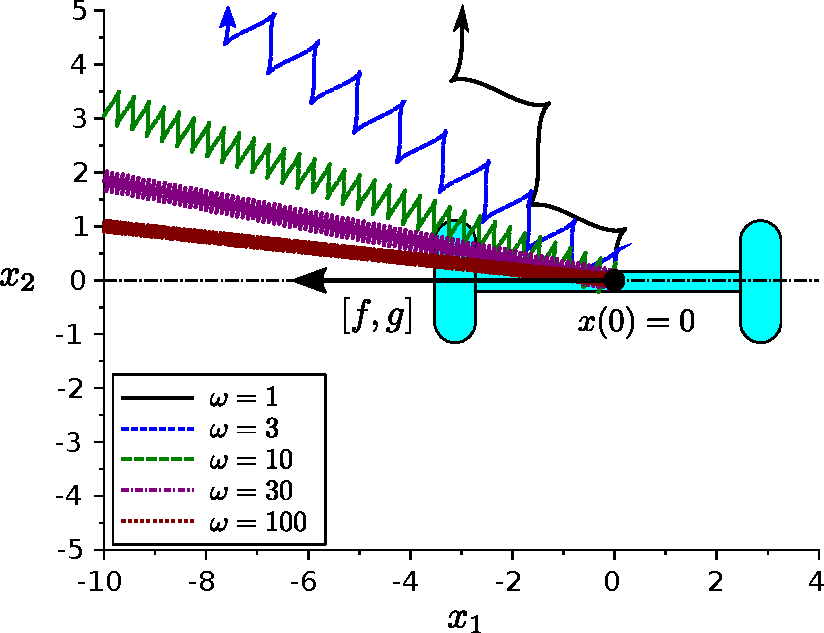
\includegraphics[width=0.75\textwidth]{roboter-averaging}
\par\end{centering}
\caption{Trajektorien des Robotermodells mit harmonischer Erregung~(\ref{eq:harmonisch-hochfreq-Erregung})
in der $(x_{1},x_{2})$-Ebene\label{fig:Trajektorien-Roboter-harmonische-Erregung}}
\end{figure}

Der Übergang von System~(\ref{eq:Umschaltsystem-zwei-VF}) mit den
Vektorfeldern~$f$ und~$g$ unter der Erregung~(\ref{eq:harmonisch-hochfreq-Erregung})
zu dem System~(\ref{eq:Lie-Klammer-harmonisch-Grenzsystem}) mit
der Lie-Klammer~$[f,g]$ lässt sich zur Steuerung bzw. Planung von
Bewegungsabläufen verwenden~\cite{sussmann1991cdc,lafferriere1993,kumar1999},
kommt aber auch in der Extremwertregelung zum Einsatz~\cite{duerr2013}.\nocite{nof1999}
Der Ansatz zur Bewegungsplanung soll für das System~(\ref{eq:Umschaltsystem-zwei-VF})
kurz erläutert werden. Durch passende Wahl der Eingänge~$u_{1}$
und~$u_{2}$ kann sich die Bahn des System~(\ref{eq:Umschaltsystem-zwei-VF})
in Richtung des Vektorfeldes~$f$ (mit $u_{1}=1,u_{2}=0$), des Vektorfeldes~$g$
(mit $u_{1}=0,u_{2}=1$) oder mit~(\ref{eq:harmonisch-hochfreq-Erregung})
in Richtung der Lie-Klammer $[f,g]$ bewegen. Prinzipiell sind auch
entsprechende Linearkombinationen der beteiligten Vektorfelder möglich.
Diese Betrachtung rechtfertigt den Übergang von dem gegebenen System~(\ref{eq:Umschaltsystem-zwei-VF})
zu dem erweiterten System (engl. \emph{Lie bracket extension})
\[
\dot{x}=v_{1}(t)f(x)+v_{2}(t)g(x)+v_{3}(t)[f,g](x)
\]
mit den neuen Eingängen $v_{1},v_{2},v_{3}$ (vgl.~\cite{sussmann1993}).
Die Bewegungsplanung auf Basis dieses Ansatzes wird beispielsweise
in~\cite{duleba1999} für das Model des mobilen Roboters erläutert.
Außerdem lässt sich dieses Mittelungsverfahren auch zur Extremalregelung
nutzen~\cite{duerr2013}.

\section{Distributionen und Kodistributionen\label{sec:Distributionen-und-Kodistributionen}}

Oft wird ein System durch mehrere gleichzeitig wirkende Vektorfelder
beschrieben, z.\,B. bei mehreren Eingängen, so dass sich das resultierende
Vektorfeld aus einer Linearkombination der beteiligten Vektorfelder
ergibt. In solchen Fällen bietet es sich an, von den einzelnen Vektorfeldern
zu dem von ihnen erzeugten geometrischem Objekt überzugehen. Dieser
Übergang führt auf das Konzept der Distribution. Die in diesem Abschnitt
enthaltene Einführung in Distributionen orientiert sich an~\cite[Abschnitt~{1.3}]{isidori3}.

Sei $\mathcal{M}\subseteq\R^{n}$ offen und $f_{1},\ldots,f_{k}:\mathcal{M}\to\R^{n}$
seien (hinreichend glatte) Vektorfelder. Diese Vektorfelder spannen
in jedem Punkt $x\in\mathcal{M}$ einen Untervektorraum des~$\R^{n}$
auf 
\begin{equation}
\spann\left\{ f_{1}(x),\ldots,f_{k}(x)\right\} ,\label{eq:VF-spannen-Dist-auf}
\end{equation}
wobei die beteiligten Vektorfelder nicht zwangsläufig linear unabhängig
sein müssen. Die Zuordnung eines Punktes $x\in\mathcal{M}$ zu einem
Untervektorraum des~$\R^{n}$ nennt man \emph{Distribution}\index{Distribution}:
\[
\mathcal{M}\ni x\mapsto\Delta(x)=\spann\left\{ f_{1}(x),\ldots,f_{k}(x)\right\} \subseteq\R^{n}.
\]
Ein Vektorfeld $f:\mathcal{M}\to\R^{n}$ liegt in der Distribution~$\Delta$,
wenn der Vektor $f(x)$ immer im Unterraum $\Delta(x)$ liegt, d.\,h.
$f\in\Delta$ bedeutet $f(x)\in\Delta(x)$ für alle $x\in\mathcal{M}$.

Wird die Distribution von glatten Vektorfeldern aufgespannt, so spricht
man von einer \emph{glatten Distribution}. Die Dimension einer Distribution~$\Delta$
im Punkt $x\in\mathcal{M}$ ist die Dimension des Unter\-vektor\-raumes
$\Delta(x)$. Eine Distribution~$\Delta$ heißt \emph{regulär}\index{Distribution!reguläre}
(im Punkt $p\in\mathcal{M}$), falls es eine Zahl $r\in\{0,\ldots,n\}$
gibt, so dass 
\[
\dim\,\Delta(x)=r
\]
 für alle~$x$ aus einer Umgebung von~$p$. Eine reguläre Distribution
hat also in der Umgebung des betreffenden Punktes eine konstante Dimension. 

Ist umgekehrt eine glatte Distribution~$\Delta$ gegeben, die im
Punkt $p\in\mathcal{M}$ regulär mit der Dimension~$r$ ist, dann
gibt es eine lokale Basisdarstellung der Distribution durch $r$ glatte
Vektorfelder~\cite[Lemma~{19.1}]{lee2006}. Genauer gesagt: Es gibt
eine Umgebung $\mathcal{U}\subseteq\mathcal{M}$ von~$p$ und $r$
glatte Vektorfelder $f_{1},\ldots,f_{r}:\mathcal{U}\to\R^{n}$ derart,
dass für alle $x\in\mathcal{U}$ gilt:
\begin{enumerate}
\item Die Vektoren $f_{1}(x),\ldots,f_{r}(x)$ sind linear unabhängig für
alle $x\in\mathcal{U}$,
\item $\Delta(x)=\spann\left\{ f_{1}(x),\ldots,f_{r}(x)\right\} $ auf~$\mathcal{U}$.
\end{enumerate}
Damit kann auf~$\mathcal{U}$ jedes Vektorfeld $f\in\Delta$ in der
Form
\begin{equation}
f(x)=\sum_{i=1}^{r}\alpha_{i}(x)f_{i}(x)\label{eq:Basisdarstellung-VF-Distr}
\end{equation}
dargestellt werden, wobei $\alpha_{1},\ldots,\alpha_{r}:\mathcal{U}\to\R$
glatte Skalarfelder sind. Gl.~(\ref{eq:Basisdarstellung-VF-Distr})
lässt sich als lineares Gleichungssystem 
\[
\left(f_{1}(x),\ldots,f_{r}(x)\right)\left(\begin{array}{c}
\alpha_{1}(x)\\
\vdots\\
\alpha_{r}(x)
\end{array}\right)=f(x)
\]
schreiben. Die Annahme $f\in\Delta$ besagt, dass das Vektorfeld~$f$
für alle $x\in\mathcal{U}$ in der linearen Hülle der Vektorfelder
$f_{1},\ldots,f_{r}$ liegt. Damit ist das lineare Gleichungssystem
lösbar.

Die Vektorfelder $f_{1},\ldots,f_{k}$ aus Gl.~(\ref{eq:VF-spannen-Dist-auf})
lassen sich spaltenweise zu einer $n\times k$-Matrix zusammenfassen:
\[
F(x)=\left(f_{1}(x),\ldots,f_{k}(x)\right).
\]
Dann gilt 
\[
\Delta(x)=\im\,F(x),
\]
so dass die Distribution von den Spalten von~$F$ aufgespannt wird.
Die Dimension der Distribution stimmt dann mit dem Rang der Matrix~$F$
überein: 
\[
\dim\,\Delta(x)=\rank\,F(x).
\]

\begin{example}
\label{exa:beispiel-distribution-rotation}Wir betrachten die von
den Vektorfeldern 
\[
f_{1}(x)=\sin x_{3}\frac{\partial}{\partial x_{1}}+\cos x_{3}\frac{\partial}{\partial x_{2}}\quad\mbox{und}\quad f_{2}(x)=-\cos x_{3}\frac{\partial}{\partial x_{1}}+\sin x_{3}\frac{\partial}{\partial x_{2}}
\]
im~$\R^{3}$ aufgespannte Distribution $\Delta=\spann\{f_{1},f_{2}\}$.
Die Vektorfelder~$f_{1}$ und~$f_{2}$ hängen von~$x_{3}$ ab,
die Distribution~$\Delta$ ist aber für ganz~$\R^{3}$ regulär mit
$\dim\,\Delta(x)=2$ und spannt für alle $x\in\R^{3}$ die $(x_{1},x_{2})$-Ebene
auf. Fasst man die Vektorfelder zu 
\[
F(x)=\left(f_{1}(x),f_{2}(x)\right)=\left(\begin{array}{cc}
\sin x_{3} & -\cos x_{3}\\
\cos x_{3} & \phantom{{-}}\sin x_{3}\\
0 & 0
\end{array}\right)
\]
zusammen, so beschreibt diese Matrix eine Rotation in der $(x_{1},x_{2}$)-Ebene
(vgl. Abb.~\ref{fig:beispiel-distribution-rotation}). Daher kann
die Beschreibung der Distribution (über die Auswahl einer Basis) zu
$\Delta=\spann\{\frac{\partial}{\partial x_{1}},\frac{\partial}{\partial x_{2}}\}$
vereinfacht werden. Die Distribution hängt damit nicht von~$x$ ab,
in jedem Punkt $x\in\mathcal{M}$ liefert $\Delta(x)$ den gleichen
Unterraum.
\end{example}
\begin{figure}
\begin{centering}
\resizebox{0.75\textwidth}{!}{\input{beispiel_distr_rotation.pdftex_t}}
\par\end{centering}
\caption{Vektorfelder $f_{1}$ und $f_{2}$ aus Beispiel~\ref{exa:beispiel-distribution-rotation}
für $p=0$ und $q=(0,0,\pi/4)^{T}$\label{fig:beispiel-distribution-rotation}}

\end{figure}

Im Bildbereich ist der Wert $\Delta(x)$ einer Distribution ein Unter\-vektor\-raum,
d.\,h. $\Delta(x)\subseteq\R^{n}$. \emph{Summe} und \emph{Durchschnitt}
von Unter\-vektor\-räumen lassen sich daher punktweise auf Distributionen
übertragen: 
\[
\begin{array}{rclcl}
\left(\Delta_{1}+\Delta_{2}\right)(x) & := & \Delta_{1}(x) & + & \Delta_{2}(x),\\
\left(\Delta_{1}\cap\Delta_{2}\right)(x) & := & \Delta_{1}(x) & \cap & \Delta_{2}(x).
\end{array}
\]
Für glatte Distributionen in der Umgebung eines regulären Punktes
sind auch Durchschnitt und Summe glatte Distributionen. Über die betreffenden
Untervektorräume im Bildbereich lassen sich auch die üblichen Teilmengen-
bzw. Unterraumrelationen für Distributionen definieren, z.\,B. 
\[
\begin{array}{rccl}
\Delta_{1}\subseteq\Delta_{2} & :\Longleftrightarrow & \forall x\in\mathcal{M}: & \Delta_{1}(x)\subseteq\Delta_{2}(x),\\
\Delta_{1}\subset\Delta_{2} & :\Longleftrightarrow & \forall x\in\mathcal{M}: & \Delta_{1}(x)\subset\Delta_{2}(x).
\end{array}
\]

Seien $\omega_{1},\ldots,\omega_{k}:\mathcal{M}\to(\R^{n})^{*}$ Kovektorfelder.
Diese spannen im Dualraum~$(\R^{n})^{*}$ des~$\R^{n}$ eine \emph{Kodistribution}\index{Kodistribution}
auf: 
\[
\Omega=\spann\left\{ \omega_{1},\ldots,\omega_{k}\right\} .
\]
 Dabei wird jedem Punkt~$x$ mit
\[
\mathcal{M}\ni x\mapsto\Omega(x)=\spann\left\{ \omega_{1}(x),\ldots,\omega_{k}(x)\right\} \subseteq(\R^{n})^{*}
\]
ein Untervektorraum des Dualraums zugeordnet. Bei Kodistributionen
sind Dimension, Summe, Durchschnitt usw. analog zu Distributionen
definiert.

\medskip{}

Für eine gegebene Distribution $\Delta$ ist der \emph{Annihilator}\index{Annihilator}
(auch \emph{Annulator}\index{Annulator} genannt)~$\Delta^{\perp}$
durch 
\[
\Delta^{\perp}(x)=\left\{ \omega\in(\R^{n})^{*};\,\left\langle \omega,f\right\rangle =0\mbox{ für alle }f\in\Delta(x)\right\} 
\]
definiert, d.\,h.~$\Delta^{\perp}$ ist eine Kodistribution. Der
Annihilator~$\Omega^{\perp}$\index{Annihilator} einer Kodistribution~$\Omega$
ist die durch 
\[
\Omega^{\perp}(x)=\left\{ f\in\R^{n};\,\left\langle \omega,f\right\rangle =0\mbox{ für alle }\omega\in\Omega(x)\right\} 
\]
definierte Distribution. Mit dem Annihilator wird der von der jeweiligen
Distribution bzw. Kodistribution erzeugte Untervektorraum um sein
orthogonales Komplement im Sinne der natürlichen Paarung ergänzt (vgl.
Abschnitt~\ref{sec:Lineare-Algebra}).

\begin{example}
\label{exa:Annihilator1}Man betrachte die von den Vektorfeldern 
\[
f_{1}(x)=\sin x_{3}\frac{\partial}{\partial x_{1}}+\cos x_{3}\frac{\partial}{\partial x_{2}}\quad\mbox{und}\quad f_{2}(x)=\frac{\partial}{\partial x_{3}}
\]
des mobilen Roboters aufgespannte Distribution $\Delta=\spann\{f_{1},f_{2}\}$.
In \textsc{Maxima} steht für die Berechnung des orthogonalen Komplements\index{orthogonales Komplement}
die Routine \hbox{\texttt{orthogonal\_complement}} zur Verfügung,
wobei die betreffenden Vektoren bzw. Vektorfelder als Spaltenvektoren
zu übergeben sind (vgl. Beispiel~\ref{exa:orthogonales-Komplement}).
Dabei liest man den Annihilator\index{Annihilator} 
\[
\Delta^{\perp}(x)=\spann\{-\cos x_{3}\,\d x_{1}+\sin x_{3}\,\d x_{2}\}
\]
ab, der zwar von Maxima als Spaltenvektor geliefert wird, hier aber
als Zeilenvektor bzw. Kovektorfeld zu verstehen ist. Die vom Programm
getroffene Zusatzannahme $\sin x_{3}\neq0$ ist der internen Implementierung
in \textsc{Maxima} geschuldet und hier nicht weiter von Bedeutung.

\begin{maxima}\noindent
%%%%%%%%%%%%%%%
%%% INPUT:
\begin{minipage}[t]{8ex}
\color{red}\bf
\begin{verbatim}
(%i1) 
\end{verbatim}
\end{minipage}
\begin{minipage}[t]{\textwidth}
\color{blue}
\begin{verbatim}
load("eigen")$
\end{verbatim}
\end{minipage}


\noindent
%%%%%%%%%%%%%%%
%%% INPUT:
\begin{minipage}[t]{8ex}
\color{red}\bf
\begin{verbatim}
(%i2) 
\end{verbatim}
\end{minipage}
\begin{minipage}[t]{\textwidth}
\color{blue}
\begin{verbatim}
f1:columnvector([sin(x3),cos(x3),0]);
\end{verbatim}
\end{minipage}
%%% OUTPUT:
\begin{math}\displaystyle
\parbox{8ex}{\color{labelcolor}(\%o2) }
\begin{pmatrix}\mathrm{sin}\left( x3\right) \cr \mathrm{cos}\left( x3\right) \cr 0\end{pmatrix}
\end{math}
%%%%%%%%%%%%%%%


\noindent
%%%%%%%%%%%%%%%
%%% INPUT:
\begin{minipage}[t]{8ex}
\color{red}\bf
\begin{verbatim}
(%i3) 
\end{verbatim}
\end{minipage}
\begin{minipage}[t]{\textwidth}
\color{blue}
\begin{verbatim}
f2:columnvector([0,0,1]);
\end{verbatim}
\end{minipage}
%%% OUTPUT:
\begin{math}\displaystyle
\parbox{8ex}{\color{labelcolor}(\%o3) }
\begin{pmatrix}0\cr 0\cr 1\end{pmatrix}
\end{math}
%%%%%%%%%%%%%%%


\noindent
%%%%%%%%%%%%%%%
%%% INPUT:
\begin{minipage}[t]{8ex}
\color{red}\bf
\begin{verbatim}
(%i4) 
\end{verbatim}
\end{minipage}
\begin{minipage}[t]{\textwidth}
\color{blue}
\begin{verbatim}
Ann:orthogonal_complement(f1,f2);
\end{verbatim}
\end{minipage}
%%% OUTPUT:
\begin{math}\displaystyle
Proviso: \mathrm{notequal}\left( \mathrm{sin}\left( x3\right) ,0\right)  \;\wedge\; \mathrm{notequal}\left( \mathrm{sin}\left( x3\right) ,0\right) 
\end{math}

\noindent
\begin{math}\displaystyle
\parbox{8ex}{\color{labelcolor}(\%o4) }
\mathrm{span}\left( \begin{pmatrix}−\mathrm{cos}\left( x3\right) \cr \mathrm{sin}\left( x3\right) \cr 0\end{pmatrix}\right) 
\end{math}
%%%%%%%%%%%%%%%

\end{maxima}
\end{example}

Den Annihilator kann man direkt über Matrizen darstellen bzw. berechnen.
Dazu fasst man die Vektorfelder $f_{1},\ldots,f_{k}:\mathcal{M}\to\R^{n}$,
welche die Distribution~$\Delta$ aufspannen, bzw. jene Kovektorfelder
$\omega_{1},\ldots,\omega_{k}:\mathcal{M}\to(\R^{n})^{*}$, die die
Kodistribution~$\Omega$ bilden, zusammen: 
\[
F(x)=\left(f_{1}(x),\ldots,f_{k}(x)\right)\quad\mbox{und}\quad W(x)=\left(\begin{array}{c}
\omega_{1}(x)\\
\vdots\\
\omega_{k}(x)
\end{array}\right).
\]
Der Annihilator~$\Delta^{\perp}$ wird von denjenigen Kovektoren~$\omega$
aufgespannt, welche die Bedingung $\omega\,F(x)=0$ erfüllen. Ähnlich
wird der Annihilator~$\Omega^{\perp}$ von Vektoren~$f$ mit $W(x)\,f=0$
aufgespannt. Das ist der Kern der Matrix~$W$, d.\,h. 
\begin{equation}
\Omega^{\perp}(x)=\ker\,W(x).\label{eq:Ann-Kern-W}
\end{equation}
Den Annihilator der Distribution~$\Delta$ erhält man mittels 
\begin{equation}
\Delta^{\perp}(x)\cong\ker\,F^{T}(x).\label{eq:Ann-Kern-FT}
\end{equation}
Da der Kern einer Matrix in Abschnitt~\ref{sec:Lineare-Algebra}
als lineare Hülle von Spaltenvektoren eingeführt wurde, der Annihilator
einer Distribution aber von Kovektorfeldern aufgespannt wird, wären
die auf der rechten Seite von~(\ref{eq:Ann-Kern-FT}) berechneten
Basisvektorfelder durch Transposition noch in den Dualraum zu übertragen.
Dabei nutzt man die Isomorphie zwischen dem Primalraum~$\R^{n}$
und seinem Dualraum~$(\R^{n})^{*}$ aus. In~(\ref{eq:Ann-Kern-FT})
wird diese Beziehung durch das Symbol ,,$\cong$`` anstelle des
Gleichheitszeichens ausgedrückt.

\begin{example}
\label{exa:Annihilator2}Wir betrachten die von den Vektorfeldern
$f_{1},f_{2}$ aufgespannte Distribution~$\Delta$ aus Beispiel~\ref{exa:Annihilator1}.
Entsprechend Gl.~(\ref{eq:Ann-Kern-FT}) lässt sich der Annihilator\index{Annihilator}
über den Kern der Matrix
\[
F^{T}(x)=\left(\begin{array}{c}
f_{1}^{T}(x)\\
f_{2}^{T}(x)
\end{array}\right)=\left(\begin{array}{ccc}
\sin x_{3} & \cos x_{3} & 0\\
0 & 0 & 1
\end{array}\right)
\]
berechnen. Die Vektorfelder werden als Listen angelegt und zeilenweise
zur Matrix~$F^{T}$ zusammengefügt. Der berechnete Annihilator stimmt
mit dem Ergebnis aus Beispiel~\ref{exa:Annihilator1} überein:

\begin{maxima}\noindent
%%%%%%%%%%%%%%%
%%% INPUT:
\begin{minipage}[t]{8ex}
\color{red}\bf
\begin{verbatim}
(%i1) 
\end{verbatim}
\end{minipage}
\begin{minipage}[t]{\textwidth}
\color{blue}
\begin{verbatim}
f1:[sin(x3),cos(x3),0];
f2:[0,0,1];
\end{verbatim}
\end{minipage}
%%% OUTPUT:
\begin{math}\displaystyle
\parbox{8ex}{\color{labelcolor}(\%o1) }
[\mathrm{sin}\left( x3\right) ,\mathrm{cos}\left( x3\right) ,0]
\end{math}

\begin{math}\displaystyle
\parbox{8ex}{\color{labelcolor}(\%o2) }
[0,0,1]
\end{math}
%%%%%%%%%%%%%%%


\noindent
%%%%%%%%%%%%%%%
%%% INPUT:
\begin{minipage}[t]{8ex}
\color{red}\bf
\begin{verbatim}
(%i3) 
\end{verbatim}
\end{minipage}
\begin{minipage}[t]{\textwidth}
\color{blue}
\begin{verbatim}
FT:matrix(f1,f2);
\end{verbatim}
\end{minipage}
%%% OUTPUT:
\begin{math}\displaystyle
\parbox{8ex}{\color{labelcolor}(\%o3) }
\begin{pmatrix}\mathrm{sin}\left( x3\right)  & \mathrm{cos}\left( x3\right)  & 0\cr 0 & 0 & 1\end{pmatrix}
\end{math}
%%%%%%%%%%%%%%%


\noindent
%%%%%%%%%%%%%%%
%%% INPUT:
\begin{minipage}[t]{8ex}
\color{red}\bf
\begin{verbatim}
(%i4) 
\end{verbatim}
\end{minipage}
\begin{minipage}[t]{\textwidth}
\color{blue}
\begin{verbatim}
Ann:nullspace(FT);
\end{verbatim}
\end{minipage}
%%% OUTPUT:
\begin{math}\displaystyle
Proviso: \mathrm{notequal}\left( \mathrm{sin}\left( x3\right) ,0\right) \;\wedge\; \mathrm{notequal}\left( \mathrm{sin}\left( x3\right) ,0\right) 
\end{math}

\noindent
\begin{math}\displaystyle
\parbox{8ex}{\color{labelcolor}(\%o4) }
\mathrm{span}\left( \begin{pmatrix}−\mathrm{cos}\left( x3\right) \cr \mathrm{sin}\left( x3\right) \cr 0\end{pmatrix}\right) 
\end{math}
%%%%%%%%%%%%%%%
\end{maxima}
\end{example}

\begin{example}
\label{exa:Annihilator3}Bei der in den Beispielen~\ref{exa:Annihilator1}
und~\ref{exa:Annihilator2} betrachteten Berechnung des Annihilators
liegt eine sehr spezielle Situation vor, nämlich eine von zwei (linear
unabhängigen) Vektorfeldern aufgespannte Distribution im Vektorraum~$\R^{3}$.
In diesem Sonderfall lässt sich über das Kreuzprodukt 
\[
f_{1}(x)\times f_{2}(x)=\left(\begin{array}{c}
\phantom{{-}}\cos x_{3}\\
-\sin x_{3}\\
0
\end{array}\right)
\]
eine Basis für den Annihilator angeben. Das Kreuzprodukt\index{Kreuzprodukt}\index{Produkt!Kreuz-}
steht senkrecht auf der von $f_{1}(x)$ und $f_{2}(x)$ aufgespannten
Ebene: 
\begin{eqnarray*}
\Delta^{\perp}(x) & = & \spann\left\{ \left(f_{1}(x)\times f_{2}(x)\right)^{T}\right\} \\
 & = & \spann\left\{ \left(\cos x_{3},-\sin x_{3},0\right)\right\} .
\end{eqnarray*}
Das gegenüber den Beispielen~\ref{exa:Annihilator1} und~\ref{exa:Annihilator2}
abweichende Vorzeichen des den Annihilator aufspannenden Kovektorfeldes
ändert nichts am Annihilator selbst. Zur Berechnung des Kreuzprodukts
steht in dem \textsc{Maxima}-Paket \texttt{vect} die binäre Operation
,,$\sim$`` zur Verfügung, die mit der Funktion \texttt{express}
ausgewertet wird:
\end{example}
\begin{maxima}\noindent
%%%%%%%%%%%%%%%
%%% INPUT:
\begin{minipage}[t]{8ex}
\color{red}\bf
\begin{verbatim}
(%i1) 
\end{verbatim}
\end{minipage}
\begin{minipage}[t]{\textwidth}
\color{blue}
\begin{verbatim}
load("vect")$
\end{verbatim}
\end{minipage}

\smallskip

\noindent
%%%%%%%%%%%%%%%
%%% INPUT:
\begin{minipage}[t]{8ex}
\color{red}\bf
\begin{verbatim}
(%i2) 
\end{verbatim}
\end{minipage}
\begin{minipage}[t]{\textwidth}
\color{blue}
\begin{verbatim}
f1:[sin(x3),cos(x3),0];
f2:[0,0,1];
\end{verbatim}
\end{minipage}
%%% OUTPUT:
\begin{math}\displaystyle
\parbox{8ex}{\color{labelcolor}(\%o2) }
[\mathrm{sin}\left( x3\right) ,\mathrm{cos}\left( x3\right) ,0]
\end{math}

\noindent
\begin{math}\displaystyle
\parbox{8ex}{\color{labelcolor}(\%o3) }
[0,0,1]
\end{math}
%%%%%%%%%%%%%%%


\noindent
%%%%%%%%%%%%%%%
%%% INPUT:
\begin{minipage}[t]{8ex}
\color{red}\bf
\begin{verbatim}
(%i4) 
\end{verbatim}
\end{minipage}
\begin{minipage}[t]{\textwidth}
\color{blue}
\begin{verbatim}
express(f1~f2);
\end{verbatim}
\end{minipage}
%%% OUTPUT:
\begin{math}\displaystyle
\parbox{8ex}{\color{labelcolor}(\%o4) }
[\mathrm{cos}\left( x3\right) ,-\mathrm{sin}\left( x3\right) ,0]
\end{math}
%%%%%%%%%%%%%%%
\end{maxima}

\begin{example}
\label{exa:Annihilator-Kodistribution}Man betrachtet das auf der
Menge $\mathcal{M}=\R^{3}\setminus\{0\}$ definierte Skalarfeld $h(x)=x_{1}^{2}+x_{2}^{2}$
, welches bereits in den Beispielen~\ref{exa:Lie-Skalar1} und~\ref{exa:Lie-Kovektor}
Verwendung fand. Der Gradient $\d h(x)=(2x_{1},2x_{2},0)$ ist ein
Kovektorfeld, welches die eindimensionale Kodistribution $\Omega:=\spann\{\d h\}$
aufspannt. Der Annihilator $\Omega^{\perp}$ ist eine zweidimensionale
Distribution 
\[
\Omega^{\perp}=\spann\left\{ -2x_{2}\frac{\partial}{\partial x_{3}},-2x_{2}\frac{\partial}{\partial x_{1}}+2x_{1}\frac{\partial}{\partial x_{2}}\right\} ,
\]
die man auf Basis von Gl.~(\ref{eq:Ann-Kern-W}) mit \textsc{Maxima}
berechnen kann:

\begin{maxima}\noindent
%%%%%%%%%%%%%%%
%%% INPUT:
\begin{minipage}[t]{8ex}
\color{red}\bf
\begin{verbatim}
(%i1) 
\end{verbatim}
\end{minipage}
\begin{minipage}[t]{\textwidth}
\color{blue}
\begin{verbatim}
h:x1^2+x2^2$
dh:jacobian([h],[x1,x2,x3]);
\end{verbatim}
\end{minipage}
%%% OUTPUT:
\begin{math}\displaystyle
\parbox{8ex}{\color{labelcolor}(\%o2) }
\begin{pmatrix}2\,x1 & 2\,x2 & 0\end{pmatrix}
\end{math}
%%%%%%%%%%%%%%%


\noindent
%%%%%%%%%%%%%%%
%%% INPUT:
\begin{minipage}[t]{8ex}
\color{red}\bf
\begin{verbatim}
(%i3) 
\end{verbatim}
\end{minipage}
\begin{minipage}[t]{\textwidth}
\color{blue}
\begin{verbatim}
D:nullspace(dh);
\end{verbatim}
\end{minipage}
%%% OUTPUT:
\begin{math}\displaystyle
Proviso: \mathrm{notequal}\left( 2\,x1,0\right) 
\end{math}

\noindent
\begin{math}\displaystyle
\parbox{8ex}{\color{labelcolor}(\%o3) }
\mathrm{span}\left( \begin{pmatrix}0\cr 0\cr -2\,x2\end{pmatrix},\begin{pmatrix}-2\,x2\cr 2\,x1\cr 0\end{pmatrix}\right) 
\end{math}
%%%%%%%%%%%%%%%
\end{maxima}
\end{example}
\medskip{}

Im Bildbereich sind Distributionen Untervektorräume. Dadurch lassen
sich gängige Eigenschaften von Unterräumen unmittelbar auf Distributionen
übertragen.
\begin{proposition}
\label{pro:Annihilator}Seien $\Delta$, $\Delta_{1}$ und $\Delta_{2}$
auf $\mathcal{M}\subseteq\R^{n}$ definierte Distributionen. Zwischen
den Distributionen und ihren Annihilatoren gelten folgende Beziehungen:
\begin{subequations}
\begin{gather}
\dim(\Delta)+\dim(\Delta^{\perp})=n\label{eq:dimensionssatz-distr-annihilator}\\
\Delta_{1}\subseteq\Delta_{2}\quad\Longleftrightarrow\quad\Delta_{1}^{\perp}\supseteq\Delta_{2}^{\perp}\label{eq:Annihilator-Subseteq}\\
\Delta_{1}\subset\Delta_{2}\quad\Longleftrightarrow\quad\Delta_{1}^{\perp}\supset\Delta_{2}^{\perp}\label{eq:eq:Annihilator-Subset}\\
\left(\Delta_{1}\cap\Delta_{2}\right)^{\perp}=\Delta_{1}^{\perp}+\Delta_{2}^{\perp}\label{eq:Annihilator-Schnitt}\\
\left(\Delta_{1}+\Delta_{2}\right)^{\perp}=\Delta_{1}^{\perp}\cap\Delta_{2}^{\perp}\label{eq:Annihilator-Summe}
\end{gather}
\end{subequations}
\end{proposition}
Gl.~(\ref{eq:dimensionssatz-distr-annihilator}) ist eine unmittelbare
Folgerung aus der Dimensions\-formel\index{Dimensionsformel}~(\ref{eq:dimensionsformel-ortho-kompl}).
Gln.~(\ref{eq:Annihilator-Subseteq}) bis~(\ref{eq:Annihilator-Summe})
ergeben sich aus den entsprechenden Aussagen für Unter\-vektor\-räume
(siehe Übungsaufgabe~\ref{aufgabe-diff-Annihilator}). \medskip{}

Bei einer glatten Distribution ist es nicht ausgeschlossen, dass es
einen lokalen Abfall der Dimension gibt, d.\,h. die Dimension in
einigen Punkten kleiner ist als in deren Umgebung. An den betreffenden
Punkten des Definitionsbereichs~$\mathcal{M}$ müsste sich nach Gl.~(\ref{eq:dimensionssatz-distr-annihilator})
die Dimension des Annihilators entsprechend erhöhen. In solchen Fällen
wäre der Annihilator nicht mehr glatt. Umgekehrt kann eine nicht glatte
Distribution durchaus einen glatten Annihilator besitzen. Derartige
pathologische Fälle sind allerdings in der Nähe eines regulären Punktes
ausgeschlossen~\cite[Lemma~{1.3.6}]{isidori3}:
\begin{lemma}
\label{lem:Annihilator-in-regulaerem-Punkt}Sei $\Delta$ eine glatte
Distribution, die im Punkt $p\in\mathcal{M}$ regulär ist. Dann ist
der Annihilator~$\Delta^{\perp}$ebenfalls im Punkt~$p$ regulär.
Außerdem gibt es eine offene Umgebung $\mathcal{U}\subseteq\mathcal{M}$
von~$p$, so dass $\Delta^{\perp}$ auf~$\mathcal{U}$ eine glatte
Kodistribution ist.
\end{lemma}

\section{Involutive Distributionen\label{sec:Involutive-Distributionen}}

Jedes glatte Vektorfeld besitzt einen eindeutigen lokalen Fluss. Fasst
man dagegen mehrere Vektorfelder in einer Distribution zusammen, so
kann die Verknüpfung der Flüsse dieser Vektorfelder möglicherweise
in eine (neue) Richtung zeigen, die nicht von den beteiligten Vektorfeldern
selber, sondern von deren Lie-Klammern aufgespannt wird (vgl. Abschnitt~\ref{sec:Lie-Klammern-dynamische-Systeme}).
Dieser Abschnitt befasst sich mit den damit verbundenen Fragestellungen,
z.\,B. unter welchen Bedingungen eine Distribution schon alle möglichen
Richtungen erfasst oder welche Konsequenzen diese Eigenschaft für
den Annihilator hat.

\medskip{}

Alle in diesem Abschnitt betrachteten Felder und Distributionen seien
auf einer offenen Teilmenge $\mathcal{M}\subseteq\R^{n}$ definiert
und hinreichend glatt. Sei $f:\mathcal{M}\to\R^{n}$ ein Vektorfeld.
Eine Distribution $\Delta$ heißt \emph{invariant}\index{Distribution!invariante}
unter dem Vektorfeld~$f$ (kurz \emph{$f$-invariant}), wenn gilt
\begin{equation}
\forall g\in\Delta:\quad[f,g]\in\Delta.\label{eq:invariant}
\end{equation}
Eine Distribution ist involutiv, wenn sie für jedes ihrer Vektorfelder
invariant ist. Genauer: Eine Distribution $\Delta$ heißt \emph{involutiv}\index{Distribution!involutive}\index{involutive Distribution},
wenn gilt 
\begin{equation}
\forall f,g\in\Delta:\quad[f,g]\in\Delta.\label{eq:involutiv}
\end{equation}
Da bei einer involutiven Distribution nach Gl.~(\ref{eq:involutiv})
auch alle Lie-Klammern der beteiligten Vektorfelder in der Distribution
liegen, ist eine involutive Distribution zugleich eine Lie-Algebra\index{Lie-Algebra}\index{Algebra!Lie-}
(vgl. Anmerkung~\ref{rem:Lie-Algebra}).

Im Abschnitt~\ref{sec:Lie-Klammern-dynamische-Systeme} wurde gezeigt,
dass die Verkettung der Flüsse zweier Vektor\-felder auch eine neue
Trajektorie generieren kann. Diese zusätzliche Bewegungsrichtung lässt
sich als Fluss der Lie-Klammern der beteiligten Vektor\-felder darstellen.
Schließt umgekehrt die betreffende Distribution entsprechend Gl.~(\ref{eq:involutiv})
die Lie-Klammern aller beteiligten Vektorfelder mit ein, so kann jede
durch Fluss\-verkettung dieser Vektorfelder erzeugte Lösungsrichtung
auch direkt von einem Vektorfeld der Distribution erzeugt werden.

Gl.~(\ref{eq:involutiv}) wäre (außer im Fall einer Distribution
der Dimension Null) für unendlich viele Vektorfelder zu prüfen, nämlich
für alle Linearkombinationen der Basisvektorfelder. Glücklicherweise
reicht es aus, die Eigenschaft~(\ref{eq:involutiv}) nur für jene
Vektorfelder, welche die Distribution aufspannen, zu verifizieren:
\begin{lemma}
\label{lem:Involutivitaetstest-mit-basis}Sei $\Delta=\spann\left\{ f_{1},\ldots,f_{r}\right\} $
mit glatten Vektorfeldern $f_{1},\ldots,f_{r}:\mathcal{M}\to\R^{n}$.
Die Distribution~$\Delta$ ist genau dann involutiv, wenn 
\begin{equation}
[f_{i},f_{j}]\in\Delta\quad\mbox{für}\quad1\leq i,j\leq r.\label{eq:involutiv-Basisvektorfelder}
\end{equation}
\end{lemma}
\begin{svmultproof2}
\notwendig\ Wenn~(\ref{eq:involutiv}) für alle Vektorfelder der
Distribution gilt, dann muss es auch für die Basisvektorfelder $f_{1},\ldots,f_{r}$
gelten, d.\,h. Bedingung~(\ref{eq:involutiv-Basisvektorfelder})
ist erfüllt.

\hinreichend\ Wegen $f,g\in\Delta$ gibt es Skalarfelder $\alpha_{1},\ldots,\alpha_{r}$
und $\beta_{1},\ldots,\beta_{r}$ mit 
\begin{eqnarray*}
f(x) & = & \sum_{i=1}^{r}\alpha_{i}(x)f_{i}(x)\\
g(x) & = & \sum_{i=1}^{r}\beta_{i}(x)f_{i}(x).
\end{eqnarray*}
Gl.~(\ref{eq:Rechenregel-LK2}) liefert 
\[
\begin{array}{rcl}
[f,g] & = & [\sum\limits _{i=1}^{r}\alpha_{i}f_{i},\sum\limits _{i=1}^{r}\beta_{i}f_{i}]\\
 & = & \sum\limits _{i=1}^{r}\sum\limits _{j=1}^{r}\left(\alpha_{i}\beta_{j}[f_{i},f_{j}]+\alpha_{i}(L_{f_{i}}\beta_{j})f_{j}-\beta_{j}(L_{f_{j}}\alpha_{i})f_{i}\right),
\end{array}
\]
d.\,h. 
\[
[f,g]\in\underbrace{\spann\left\{ f_{1},\ldots,f_{r}\right\} }_{{\displaystyle =\Delta}}+\underbrace{\spann\left\{ [f_{i},f_{j}],\;1\leq i,j\leq r\right\} }_{{\displaystyle \subseteq\Delta\mbox{ wegen }(\ref{eq:involutiv-Basisvektorfelder})}}=\Delta,
\]
also gilt~(\ref{eq:involutiv}).
\end{svmultproof2}

Die Involutivitätsbedingung aus Lemma~\ref{lem:Involutivitaetstest-mit-basis}
lässt sich leicht implementieren (siehe Alg.~\ref{alg:Test-Involutivitaet}).
Der \textsc{Maxima}-Funktion \texttt{Involutivep} wird die zu prüfende
Distribution als eine Liste von Vektorfeldern $f_{1},\ldots,f_{r}$
übergeben und in eine Matrix umgewandelt. Bei Hinzunahme von Lie-Klammern
$[f_{i},f_{j}]$ darf sich im Falle einer involutiven Distribution
der Rang nicht erhöhen. Aufgrund der Schiefsymmetrie der Lie-Klammer
(siehe Prop.~\ref{prop:Eigenschaften-Lie-Klammer}) genügt es, die
Lie-Klammern $[f_{i},f_{j}]$ für $i=1,\ldots,r$ und $j=i+1,\ldots,r$
zu prüfen.

\begin{algorithm}
\noindent
%%%%%%%%%%%%%%%
%%% INPUT:
%\begin{minipage}[t]{8ex}
%\color{red}\bf
%\begin{verbatim}
%(%i11) 
%\end{verbatim}
%\end{minipage}
\begin{minipage}[t]{\textwidth}
\color{blue}
\begin{verbatim}
Involutivep(L,x):=block([F,G,i,j,r],
    r:length(L),
    F:apply('matrix,L),
    F:transpose(F),
    G:copy(F),  
    for i:1 thru r do 
        for j:i+1 thru r do block([f1,f2],
            f1:list_matrix_entries(col(F,i)),
            f2:list_matrix_entries(col(F,j)),
            G:addcol(G,LieBracket(f1,f2,x))
    ),
    is(rank(F)=rank(G))
)$
\end{verbatim}
\end{minipage}


\caption{Test eines Distribution auf Involutivität\label{alg:Test-Involutivitaet}}

\end{algorithm}

\begin{example}
\label{exa:Roboter-Test-Involutivitaet}Die von den Vektorfeldern
\[
f_{1}(x)=\sin x_{3}\frac{\partial}{\partial x_{1}}+\cos x_{3}\frac{\partial}{\partial x_{2}}\quad\mbox{und}\quad f_{2}(x)=\frac{\partial}{\partial x_{3}}
\]
des mobilen Roboters aufgespannte Distribution $\Delta=\spann\{f_{1},f_{2}\}$
ist auf Involutitvität zu untersuchen. Die Lie-Klammer der die Distribution
aufspannenden Vektorfelder~$f_{1}$ und~$f_{2}$ wurde bereits in
Beispiel~\ref{exa:Lie-Vektorfeld-Roboter} berechnet:
\[
[f_{1},f_{2}]=-\cos x_{3}\frac{\partial}{\partial x_{1}}+\sin x_{3}\frac{\partial}{\partial x_{2}}
\]
Wir fassen die drei Vektorfelder zu einer Matrix zusammen: 
\[
F(x)=\left(f_{1}(x),f_{2}(x),[f_{1},f_{2}](x)\right)=\left(\begin{array}{ccc}
\sin x_{3} & 0 & -\cos x_{3}\\
\cos x_{3} & 0 & \phantom{{-}}\sin x_{3}\\
0 & 1 & 0
\end{array}\right).
\]
Wegen $\det F(x)\equiv-1$ sind die beteiligten Vektorfelder linear
unabhängig. Daher lässt sich die Lie-Klammer $[f_{1},f_{2}]$ nicht
als Linearkombination der Vektorfelder $f_{1},f_{2}$ darstellen,
also gilt $[f_{1},f_{2}]\notin\Delta$. Die Distribution~$\Delta$
ist daher nicht involutiv.

Für die Überprüfung mit \textsc{Maxima} definiert man die Vektorfelder~$f_{1},f_{2}$
sowie~$x$ als Listen. Die Distribution $\Delta=\spann\{f_{1},f_{2}\}$,
die als Liste der Vektorfelder~$f_{1}$ und~$f_{2}$ an die in Alg.~\ref{alg:Test-Involutivitaet}
definierte \textsc{Maxima}-Funktion \texttt{Involtuivep} übergeben
wird, ist (wie bereits festegestellt wurde) nicht involutiv. Ergänzt
man die Distribution~$\Delta$ um die Lie-Klammer $[f_{1},f_{2}]$,
so erhält man eine involutive Distribution:

\begin{maxima}\noindent
%%%%%%%%%%%%%%%
%%% INPUT:
\begin{minipage}[t]{8ex}
\color{red}\bf
\begin{verbatim}
(%i5) 
\end{verbatim}
\end{minipage}
\begin{minipage}[t]{\textwidth}\color{blue}
\begin{verbatim}
f1:[sin(x3),cos(x3),0];
f2:[0,0,1];
x:[x1,x2,x3];
\end{verbatim}
\end{minipage}
%%% OUTPUT:
\begin{math}\displaystyle
\parbox{8ex}{\color{labelcolor}(\%o3) }
[\mathrm{sin}\left( x3\right) ,\mathrm{cos}\left( x3\right) ,0]
\end{math}

\noindent
\begin{math}\displaystyle
\parbox{8ex}{\color{labelcolor}(\%o4) }
[0,0,1]
\end{math}

\noindent
\begin{math}\displaystyle
\parbox{8ex}{\color{labelcolor}(\%o5) }
[x1,x2,x3]
\end{math}
%%%%%%%%%%%%%%%

\noindent
%%%%%%%%%%%%%%%
%%% INPUT:
\begin{minipage}[t]{8ex}
\color{red}\bf
\begin{verbatim}
(%i7) 
\end{verbatim}
\end{minipage}
\begin{minipage}[t]{\textwidth}
\color{blue}
\begin{verbatim}
D:[f1,f2];
Involutivep(D,x);
\end{verbatim}
\end{minipage}

%%% OUTPUT:
\noindent
\begin{math}\displaystyle
\parbox{8ex}{\color{labelcolor}(\%o6) }
[[\mathrm{sin}\left( x3\right) ,\mathrm{cos}\left( x3\right) ,0],[0,0,1]]
\end{math}

\noindent
\begin{math}\displaystyle
\parbox{8ex}{\color{labelcolor}(\%o7) }
false
\end{math}
%%%%%%%%%%%%%%%


\noindent
%%%%%%%%%%%%%%%
%%% INPUT:
\begin{minipage}[t]{8ex}
\color{red}\bf
\begin{verbatim}
(%i9) 
\end{verbatim}
\end{minipage}
\begin{minipage}[t]{\textwidth}
\color{blue}
\begin{verbatim}
I:endcons(LieBracket(f1,f2,x),D);
Involutivep(I,x);
\end{verbatim}
\end{minipage}

%%% OUTPUT:
\noindent
\begin{math}\displaystyle
\parbox{8ex}{\color{labelcolor}(\%o8) }
[[\mathrm{sin}\left( x3\right) ,\mathrm{cos}\left( x3\right) ,0],[0,0,1],[-\mathrm{cos}\left( x3\right) ,\mathrm{sin}\left( x3\right) ,0]]
\end{math}

\noindent
\begin{math}\displaystyle
\parbox{8ex}{\color{labelcolor}(\%o9) }
true
\end{math}
%%%%%%%%%%%%%%%
\end{maxima}
\end{example}

Involutive Distributionen können immer von kommutierenden Vektorfeldern
aufgespannt werden:
\begin{lemma}
\label{lem:Basisdarstellung-involutive-Distribution}Die Distribution~$\Delta$
sei involutiv und im Punkt $p\in\mathcal{M}$ regulär mit der Dimension~$r$.
Dann existieren eine Umgebung $\mathcal{U}\subseteq\mathcal{M}$ von~$p$
und Vektorfelder $g_{1},\ldots,g_{r}:\mathcal{U}\to\R^{n}$ derart,
dass auf~$\mathcal{U}$ gilt $\Delta=\spann\left\{ g_{1},\ldots,g_{r}\right\} $
und 
\[
\forall x\in\mathcal{U}:\quad[g_{i},g_{j}]=0\quad\mbox{für}\quad1\leq i,j\leq r.
\]
\end{lemma}

Die Beweisidee entstammt~\cite[S.~131-132]{jakubczyk2001course}.
\begin{svmultproof2}
Sei $r=\dim\Delta(p)$. Dann gibt es $r$ linear unabhängige Vektorfelder
$f_{1},\ldots,f_{r}$, die lokal (d.\,h. auf einer Umgebung~$\mathcal{U}$
von~$p$) die Distribution~$\Delta$ aufspannen. Für die $n\times r$-Matrix
\[
F(x)=\left(f_{1}(x),\ldots,f_{r}(x)\right)
\]
gilt $\Delta(x)=\im\,F(x)$ und $\rank\,F(x)=r$. Folglich gibt es
eine reguläre $r\times r$-Teilmatrix $B(x)$ von $F(x)$. Ohne Einschränkung
setze sich $B(x)$ aus den ersten $r$ Zeilen von $F(x)$ zusammen
(andernfalls Umnumerierung der Koordinaten im Bildbereich). Über die
Rechtsmultiplikation mit~$B^{-1}(x)$
\[
F(x)B^{-1}(x)=\left(\begin{array}{ccc}
 & B(x)\\
\hline * & \cdots & *\\
\vdots & \ddots & \vdots\\
* & \cdots & *
\end{array}\right)B^{-1}(x)=\left(\begin{array}{ccc}
 & I_{r}\\
\hline * & \cdots & *\\
\vdots & \ddots & \vdots\\
* & \cdots & *
\end{array}\right)=:\left(g_{1}(x),\ldots,g_{r}(x)\right)
\]
definiert man die neuen Vektorfelder $g_{1},\ldots,g_{r}$, lässt
aber den aufgespannten Raum unverändert. Andererseits ist~$\Delta$
involutiv, d.\,h. für jedes Paar $(i,j)$ gibt es Skalarfelder $\alpha_{1},\ldots,\alpha_{r}$
mit 
\[
[g_{i},g_{j}](x)=\alpha_{1}(x)g_{1}(x)+\cdots+\alpha_{r}(x)g_{r}(x).
\]
Dieses Gleichungssystem hat die Form 
\[
\left(\begin{array}{c}
0\\
\vdots\\
\vdots\\
0\\
\hline *\\
\vdots\\
*
\end{array}\right)=\alpha_{1}(x)\left(\begin{array}{c}
1\\
0\\
\vdots\\
0\\
\hline *\\
\vdots\\
*
\end{array}\right)+\cdots+\alpha_{r}(x)\left(\begin{array}{c}
0\\
\vdots\\
0\\
1\\
\hline *\\
\vdots\\
*
\end{array}\right).
\]
Da die Vektorfelder $g_{1},\ldots,g_{r}$ in den ersten $r$ Zeilen
konstant sind, enthält die Lie-Klammer $[g_{i},g_{j}]$, die die linke
Seite des Gleichungssystems bildet, in diesen Zeilen immer die Nullfunktion.
Der Vergleich der ersten $r$ Zeilen des Gleichungssystems liefert
$\alpha_{1}=\cdots=\alpha_{r}=0$ auf~$\mathcal{U}$ und damit insgesamt
$[g_{i},g_{j}]=0$.
\end{svmultproof2}

\begin{theorem}
[Simultane Begradigung von Vektorfeldern]\index{Satz!von der simultanen Begradigung von Vektorfeldern}\label{thm:simultane-begradigung-von-VF}Sei
$p\in\mathcal{M}$. Für die Vektor\-felder $f_{1},\ldots,f_{r}:\mathcal{M}\to\R^{n}$
gelte

\begin{enumerate}
\item $f_{1}(x),\ldots,f_{r}(x)$ sind linear unabhängig und
\item $[f_{i},f_{j}](x)=0$, $1\leq i,j\leq r$
\end{enumerate}
für alle $x$ aus einer Umgebung von~$p$. Dann existiert ein lokaler
Diffeomorphismus\index{Diffeomorphismus} $z=T(x)$ mit $T(p)=0$,
so dass gilt 
\[
\left.T_{*}f_{i}(x)\right|_{x=T^{-1}(z)}=\frac{\partial}{\partial z_{i}},\quad1\leq i\leq r
\]
 für alle $z$ aus einer Umgebung von Null.
\end{theorem}
\begin{svmultproof2}
Zu den linear unabhängigen Vektorfeldern $f_{1},\ldots,f_{r}$ gibt
es $n-r$ weitere Vektor\-felder $f_{r+1},\ldots,f_{n}:\mathcal{U}\to\R^{n}$,
so dass $f_{1},\ldots,f_{n}$ in einer Umgebung von~$p$ linear unabhängig
sind. Wir definieren eine Abbildung~$S$ durch die Verkettung der
Flüsse dieser Vektorfelder:\index{Fluss!Verkettung}
\begin{equation}
x=S(z):=\varphi_{z_{1}}^{f_{1}}\circ\cdots\circ\varphi_{z_{n}}^{f_{n}}(p).\label{eq:S-flussverknuepfung}
\end{equation}
Eine Reihentwicklung nach~$z$ liefert 
\[
x=p+f_{1}(p)z_{1}+\cdots+f_{n}(p)z_{n}+\mathcal{O}(\|z\|^{2}).
\]
Wegen der linearen Unabhängigkeit von $f_{1}(p),\ldots,f_{n}(p)$
(Annahme~1) ist die Jacobimatrix 
\[
S^{\prime}(0)=\left(f_{1}(p),\ldots,f_{n}(p)\right)
\]
regulär. Daher ist $S$ ein lokaler Diffeomorphismus, dessen Umkehrabbildung
im Folgenden mit $z=T(x)$ bezeichnet wird. Wegen Annahme~2 und Lemma~\ref{lem:kommutierende-fluesse}
gilt für $i=1,\ldots,r$:
\[
\begin{array}{ccl}
S^{\prime}(z)\frac{\partial}{\partial z_{i}} & = & \frac{\partial}{\partial z_{i}}S(z)\\
 & = & \frac{\partial}{\partial z_{i}}\varphi_{z_{1}}^{f_{1}}\circ\cdots\circ\varphi_{z_{i}}^{f_{i}}\circ\cdots\circ\varphi_{z_{n}}^{f_{n}}(p)\\
 & = & \frac{\partial}{\partial z_{i}}\varphi_{z_{i}}^{f_{i}}\circ\varphi_{z_{1}}^{f_{1}}\circ\cdots\circ\varphi_{z_{i-1}}^{f_{i-1}}\circ\varphi_{z_{i+1}}^{f_{i+1}}\circ\cdots\circ\varphi_{z_{n}}^{f_{n}}(p)\\
 & = & f_{i}\left(\varphi_{z_{i}}^{f_{i}}\circ\varphi_{z_{1}}^{f_{1}}\circ\cdots\circ\varphi_{z_{i-1}}^{f_{i-1}}\circ\varphi_{z_{i+1}}^{f_{i+1}}\circ\cdots\circ\varphi_{z_{n}}^{f_{n}}(p)\right)\\
 & = & f_{i}\left(\varphi_{z_{1}}^{f_{1}}\circ\cdots\circ\varphi_{z_{i}}^{f_{i}}\circ\cdots\circ\varphi_{z_{n}}^{f_{n}}(p)\right)\\
 & = & f_{i}(S(z))\\
 & = & \left.f_{i}(x)\right|_{x=S(z)}.
\end{array}
\]
Dann gilt 
\[
S^{\prime}(z)\frac{\partial}{\partial z_{i}}=\left.f_{i}(x)\right|_{x=S(z)}
\]
bzw. die wegen $S=T^{-1}$ gleichwertige Aussage 
\[
\frac{\partial}{\partial z_{i}}=\left.T^{\prime}(x)f_{i}(x)\right|_{x=T^{-1}(z)}
\]
für $i=1,\ldots,r$.
\end{svmultproof2}

Die im Satz~\ref{thm:simultane-begradigung-von-VF} beschriebene
simultane Begradigung wird für den Fall $n=r=2$ in Abb.~\ref{fig:Simultane-Begradigung-zweier-VF}
illustriert.

\begin{figure}
\begin{centering}
\input{simult_begrad1.pdftex_t}
\par\end{centering}
\caption{Simultane Begragigung zweier Vektorfelder im~$\R^{2}$\label{fig:Simultane-Begradigung-zweier-VF}}
\end{figure}

\begin{corollary}
[Begradigung einer Nichtruhelage]\label{cor:begradigung-einer-Nichtruhelage}Seien
$f:\mathcal{M}\to\R^{n}$ und $p\in\mathcal{M}$ mit $f(p)\neq0$.
Dann gibt es in der Umgebung von~$p$ einen lokalen Diffeomorphismus
$z=T(x)$ mit 
\[
\left.T^{\prime}(x)f(x)\right|_{x=T^{-1}(z)}=\frac{\partial}{\partial z_{1}}.
\]
\end{corollary}
\begin{svmultproof2}
Der Vektor $f(p)\neq0$ ist linear unabhängig. Außerdem gilt $[f,f]=0$
für jedes differenzierbare Vektorfeld~$f$. Damit kann Satz~\ref{thm:simultane-begradigung-von-VF}
mit $r=1$ angewendet werden.
\end{svmultproof2}

In der Umgebung einer Nichtruhelage ist die Differentialgleichung
$\dot{x}=f(x)$ somit topologisch konjugiert zur Differentialgleichung
\[
\dot{z}_{1}=1,\;\dot{z}_{2}=0,\;\ldots,\;\dot{z}_{n}=0,
\]
deren rechte Seite ein Einheitsvektor ist.

\begin{example}
Die Begradigung einer Nichtruhelage wird am Beispiel des folgenden
linearen Vektorfeldes bzw. des Differentialgleichungssystems 
\begin{equation}
\dot{x}=f(x)=\left(\begin{array}{r}
x_{1}\\
-x_{2}
\end{array}\right)\label{eq:beispiel-begrad-nichtruhelage}
\end{equation}
verdeutlicht. Das Phasenportrait ist in Abb.~\ref{fig:beispiel-begrad-nichtruhelage}
(links) zu sehen. Das System~(\ref{eq:beispiel-begrad-nichtruhelage})
hat im Ursprung $x=0$ eine Ruhelage. Die Begradigung soll im Punkt
$p=(1,1)^{T}$ erfolgen, wo $f(p)\neq0$ gilt (Nichtruhelage). Die
Berechnung der Koordinatentransformation erfolgt mit Gl.~(\ref{eq:S-flussverknuepfung})
(vgl. Beweis von Satz~\ref{thm:simultane-begradigung-von-VF}). Dazu
wird das gegebene Vektorfeld $f_{1}:=f$ durch ein weiteres Vektorfeld~$f_{2}$
ergänzt, so dass beide Vektorfelder im Punkt~$p$ linear unabhängig
sind. Zur Ergänzung wählen wir das sehr einfache Vektorfeld $f_{2}(x)=(0,1)^{T}$.
Die Flüsse der beiden Vektorfelder lauten 
\[
\varphi_{t}^{f_{1}}(x)=\left(\begin{array}{c}
\e^{t}x_{1}\\
\e^{-t}x_{2}
\end{array}\right)\quad\text{und}\quad\phi_{t}^{f_{2}}(x)=\left(\begin{array}{c}
x_{1}\\
x_{2}+t
\end{array}\right),
\]
womit man durch die Flussverkettung nach Gl.~(\ref{eq:S-flussverknuepfung})
die Rücktransformation
\[
x=S(z)=\varphi_{z_{1}}^{f_{1}}\circ\varphi_{z_{2}}^{f_{2}}(p)=\varphi_{z_{1}}^{f_{1}}\circ\left(\begin{array}{c}
1\\
1+z_{2}
\end{array}\right)=\left(\begin{array}{c}
\e^{z_{1}}\\
\e^{-z_{1}}(1+z_{2})
\end{array}\right)
\]
erhält. Durch Auflösen dieser Gleichung nach~$z$ ergibt sich die
Hintransformation 
\begin{equation}
z=T(x)=\left(\begin{array}{c}
\ln x_{1}\\
x_{1}x_{2}-1
\end{array}\right)\quad\text{mit}\quad T^{\prime}(x)=\left(\begin{array}{cc}
\frac{1}{x_{1}} & 0\\
x_{2} & x_{1}
\end{array}\right),\label{eq:beispiel-begrad-T}
\end{equation}
mit der das Vektorfeld~$f$ bzw. System~(\ref{eq:beispiel-begrad-nichtruhelage})
um den Punkt~$p$ in die Form 
\begin{eqnarray*}
\dot{z} & = & T_{*}f(S(z))\\
 & = & \left.T^{\prime}(x)f(x)\right|_{x=S(z)}\\
 & = & \left.\left(\begin{array}{cc}
\frac{1}{x_{1}} & 0\\
x_{2} & x_{1}
\end{array}\right)\left(\begin{array}{r}
x_{1}\\
-x_{2}
\end{array}\right)\right|_{x=S(z)}\\
 & = & \left(\begin{array}{c}
1\\
0
\end{array}\right)
\end{eqnarray*}
des ersten Einheitsvektors überführt wird (vgl. Abb.~\ref{fig:beispiel-begrad-nichtruhelage}
(rechts)).
\end{example}
\begin{figure}
\begin{centering}
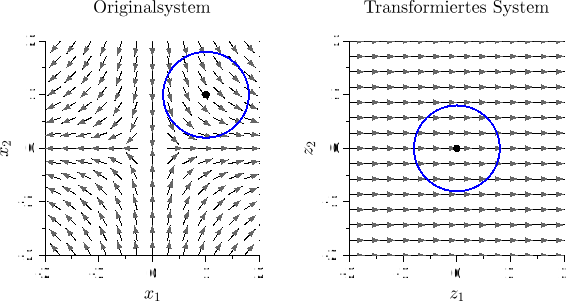
\includegraphics[width=0.95\textwidth]{beispiel_begradigung_nichtruhelage1}
\par\end{centering}
\caption{Phasenportraits von System~(\ref{eq:beispiel-begrad-nichtruhelage})
und dem transformierten System \label{fig:beispiel-begrad-nichtruhelage}}

\end{figure}

Die Vektorfelder $\tfrac{\partial}{\partial z_{1}},\ldots,\tfrac{\partial}{\partial z_{r}}$
aus Satz~\ref{thm:simultane-begradigung-von-VF} können mit den weiteren
Vektor\-feldern $\tfrac{\partial}{\partial z_{r+1}},\ldots,\tfrac{\partial}{\partial z_{n}}$
(als orthogonales Komplement\index{orthogonales Komplement}, siehe
Abschnitt~\ref{sec:Lineare-Algebra}) zu einer Basis des Tangentialraums
ergänzt werden. Diese Tatsache führt zu folgender Erkenntnis:
\begin{corollary}
\label{cor:ergaenzung-einer-involutiven-distribution}Die Distribution~$\Delta$
sei involutiv und im Punkt $p\in\mathcal{M}$ regulär mit $\dim\Delta=r$.
Dann existieren eine Umgebung $\mathcal{U}\subseteq M$ von~$p$
und $n-r$ Vektorfelder $f_{r+1},\ldots,f_{n}:\mathcal{U}\to\R^{n}$,
so dass
\[
\Delta(x)\oplus\spann\left\{ f_{r+1}(x),\ldots,f_{n}(x)\right\} =\R^{n}
\]
für alle $x\in\mathcal{U}$.
\end{corollary}
\begin{svmultproof2}
Auf Basis von Satz~\ref{thm:simultane-begradigung-von-VF} können
die $r$~Vektorfelder, welche die involutive Distribution~$\Delta$
aufspannen, mit einer Transformation~$T$ in die Form $\tfrac{\partial}{\partial z_{1}},\ldots,\tfrac{\partial}{\partial z_{r}}$
überführt werden. Die von den zusätzlichen Vektorfeldern $\tfrac{\partial}{\partial z_{r+1}},\ldots,\tfrac{\partial}{\partial z_{n}}$
aufgespannte Distribution ist involutiv, weil die Vektorfelder konstant
sind. Die Involutivität bleibt wegen Prop.~\ref{pro:Lie-Klammer-und-Push-Forward}
unter Rücktransformation~$S$ erhalten, wobei die Vektor\-felder
$\tfrac{\partial}{\partial z_{j}}$ dann die Form 
\[
f_{j}(x):=\left.S^{\prime}(z)\tfrac{\partial}{\partial z_{j}}\right|_{z=T(x)}
\]
 für $j=r+1,\ldots,n$ annehmen.
\end{svmultproof2}

Nachfolgend geht es um die Frage, welche Auswirkungen die Involutivität
einer Distribution auf den Annihilator hat.
\begin{definition}
\label{def:Integrierbarkeit-Distribution}Eine reguläre Distribution~$\Delta$
mit $\dim\Delta=r$ heißt \emph{integrierbar}\index{Distribution!integrierbare},
wenn es Skalarfelder $\lambda_{1},\ldots,\lambda_{n-r}$ gibt, so
dass 
\begin{equation}
\Delta^{\perp}=\spann\left\{ \d\lambda_{1},\ldots,\d\lambda_{n-r}\right\} .\label{eq:Distr-def-integrierbar}
\end{equation}
Die Besonderheit einer integrierbaren Distribution besteht also demnach
darin, dass der Annihilator nicht von beliebigen Kovektorfeldern aufgespannt
wird, sondern von exakten Differentialen (d.\,h. von Gradienten\index{Gradient}).
\end{definition}
\begin{theorem}
[Satz von Frobenius]\label{thm:Frobenius-lokal}\index{Satz!von Frobenius}Die
Distribution~$\Delta$ sei im Punkt $p\in\mathcal{M}$ regulär.\index{Distribution!reguläre}\index{Distribution!involutive}
In einer geeigneten Umgebung~$\mathcal{U}$ von~$p$ gilt dann:
\[
\Delta\mbox{ ist involutiv}\quad\Longleftrightarrow\quad\Delta\mbox{ ist integrierbar.}
\]
\end{theorem}
\begin{svmultproof2}
Da die Distribution regulär ist, gibt es $r=\dim\Delta$ linear unabhängige
Vektor\-felder $f_{1},\ldots,f_{r}:\mathcal{U}{\to\R}^{n}$ mit $\Delta=\spann\{f_{1},\ldots,f_{r}\}$.

\hinreichend\ Nach Lemma~\ref{lem:Basisdarstellung-involutive-Distribution}
können die Vektorfelder so gewählt werden, dass 
\[
[f_{i},f_{j}]\equiv0\quad\mbox{für}\quad1\leq i,j\leq r.
\]
Nach dem Begradigungssatz~\ref{thm:simultane-begradigung-von-VF}
existiert ein lokaler Diffeomorphismus $z=T(x)$ mit $T=(t_{1},\ldots,t_{n})^{T}$,
so dass
\[
\left.T^{\prime}(x)f_{i}(x)\right|_{x=T^{-1}(z)}=\frac{\partial}{\partial z_{i}}\quad\mbox{für}\quad i=1,\ldots,r.
\]
Dadurch werden die Vektorfelder in Richtung der Einheisvektoren $\tfrac{\partial}{\partial z_{1}},\ldots,\tfrac{\partial}{\partial z_{r}}$
ausgerichtet. Die Kovektoren $\d z_{r+1},\ldots,\d z_{n}$ der dualen
Basis sind dazu orthogonal, d.\,h. 
\[
\left\langle \d z_{j},\frac{\partial}{\partial z_{i}}\right\rangle =0\quad\mbox{für}\quad\begin{array}{ccl}
i & = & 1,\ldots,r,\\
j & = & r+1,\ldots,n.
\end{array}
\]
Dann gilt
\[
\begin{array}{ccl}
0 & = & \left\langle \d z_{j},\frac{\partial}{\partial z_{i}}\right\rangle \\
 & = & \left\langle \d z_{j},T^{\prime}(x)f_{i}(x)\right\rangle \\
 & = & \left\langle \d z_{j}T^{\prime}(x),f_{i}(x)\right\rangle \\
 & = & \left\langle \d t_{j}(x),f_{i}(x)\right\rangle 
\end{array}
\]
für $i=1,\ldots,r$ und $j=r+1,\ldots,n$, wobei $\d t_{j}$ die $j$-te
Zeile der Jacobi\-matrix~$T^{\prime}$ darstellt. Die Kovektorfelder
$\d t_{r+1},\ldots,\d t_{n}$ sind also orthogonal zu den die Distribution
aufspannenden Vektorfeldern $f_{1},\ldots,f_{r}$ und damit Elemente
des Annihilators~$\Delta^{\perp}$. Aufgrund des Begradigungssatzes
ist~$T$ ein Diffeomorphismus, insbesondere ist $T^{\prime}(p)$
regulär. Damit sind die Zeilen $\d t_{r+1},\ldots,\d t_{n}$ in der
Umgebung von~$p$ linear unabhängig. Die Differentiale $\d\lambda_{k}$
mit $\lambda_{k}=t_{r+k}$ für $k=1,\ldots,n-r$ spannen folglich~$\Delta^{\perp}$
auf, d.\,h. es gilt~(\ref{eq:Distr-def-integrierbar}). Damit ist~$\Delta$
integrierbar.

\notwendig\ Die Distribution~$\Delta$ sei integrierbar, d.\,h.
es gibt Skalarfelder $\lambda_{1},\ldots,\lambda_{n-r}$ mit~(\ref{eq:Distr-def-integrierbar}).
Daher gilt 
\[
L_{f_{i}}\lambda_{j}=\left\langle \d\lambda_{j},f_{i}\right\rangle =0\quad\mbox{für}\quad\begin{array}{ccl}
i & = & 1,\ldots,r,\\
j & = & r+1,\ldots,n.
\end{array}
\]
Weitere Lie-Ableitungen entlang~$f_{k}$ sind ebenfalls Null: 
\[
L_{f_{k}}L_{f_{i}}\lambda=\langle\underbrace{\d L_{f_{i}}\lambda_{j}}_{{\displaystyle =0}},f_{k}\rangle=0\quad\mbox{für}\quad1\leq i,k\leq r.
\]
Daher gilt 
\[
L_{[f_{i},f_{k}]}\lambda_{j}=L_{f_{i}}L_{f_{k}}\lambda_{j}-L_{f_{k}}L_{f_{i}}\lambda_{j}=0.
\]
Für $j=1,\ldots,n-r$ erhält man 
\[
\left(\begin{array}{c}
L_{[f_{i},f_{k}]}\lambda_{1}\\
\vdots\\
L_{[f_{i},f_{k}]}\lambda_{n-r}
\end{array}\right)=\left(\begin{array}{c}
\d\lambda_{1}\\
\vdots\\
\d\lambda_{n-r}
\end{array}\right)[f_{i},f_{k}]=0.
\]
Die Kovektorfelder $\d\lambda_{1},\ldots,\d\lambda_{n-r}$ spannen
laut Annahme den Annihilator von~$\Delta$ auf. Die Lie-Klammern
$[f_{i},f_{k}]$ stehen senkrecht auf der Basis von~$\Delta^{\perp}$
und gehören damit zu~$\Delta$, d.\,h. $[f_{i},f_{k}]\in\Delta$.
Also ist~$\Delta$ involutiv.
\end{svmultproof2}

\begin{example}
\label{exa:Frobenius1}Man betrachte die von den Vektorfeldern 
\[
f_{1}(x)=-2x_{2}\frac{\partial}{\partial x_{3}}\quad\text{und}\quad f_{2}(x)=-2x_{2}\frac{\partial}{\partial x_{1}}+2x_{1}\frac{\partial}{\partial x_{2}}
\]
auf der Menge $\mathcal{M}=\left\{ x\in\R^{3};\;x_{1}\neq0\wedge x_{2}\neq0\right\} $
aufgespannte Distribution $\Delta=\spann\{f_{1},f_{2}\}.$ Diese Distribution~$\Delta$
kann man auch in der Form 
\[
\Delta(x)=\im\,F(x)\quad\text{mit}\quad F(x)=\left(f_{1}(x),f_{2}(x)\right)=\left(\begin{array}{cc}
0 & -2x_{2}\\
0 & \phantom{{-}}2x_{1}\\
-2x_{2} & 0
\end{array}\right)
\]
beschreiben, wobei die Matrix $F(x)$ für alle $x\in\mathcal{M}$
den Rang~$2$ aufweist. Folglich ist die Distribution regulär mit
$\dim\Delta=2$. Außerdem ist die Distribution wegen 
\[
[f_{1},f_{2}](x)=4x_{1}\frac{\partial}{\partial x_{3}}=-2\frac{x_{1}}{x_{2}}(-2x_{2})\frac{\partial}{\partial x_{3}}=-2\frac{x_{1}}{x_{2}}f_{1}(x)\in\Delta(x)
\]
involutiv (vgl. Lemma~\ref{lem:Involutivitaetstest-mit-basis}),
so dass die Voraussetzung von Satz~\ref{thm:Frobenius-lokal} erfüllt
sind. Eine mögliche Basis des Annihilators lässt sich mit \textsc{Maxima}
berechnen:

\begin{maxima}\noindent
%%%%%%%%%%%%%%%
%%% INPUT:
\begin{minipage}[t]{8ex}
\color{red}\bf
\begin{verbatim}
(%i1) 
\end{verbatim}
\end{minipage}
\begin{minipage}[t]{\textwidth}
\color{blue}
\begin{verbatim}
load(eigen)$
\end{verbatim}
\end{minipage}

\smallskip

\noindent
%%%%%%%%%%%%%%%
%%% INPUT:
\begin{minipage}[t]{8ex}
\color{red}\bf
\begin{verbatim}
(%i2) 
\end{verbatim}
\end{minipage}
\begin{minipage}[t]{\textwidth}
\color{blue}
\begin{verbatim}
f1:columnvector([0,0,-2*x2])$
f2:columnvector([-2*x2,2*x1,0])$
F:addcol(f1,f2);
\end{verbatim}
\end{minipage}
%%% OUTPUT:
\begin{math}\displaystyle
\parbox{8ex}{\color{labelcolor}(\%o4) }
\begin{pmatrix}0 & -2\,x2\cr 0 & 2\,x1\cr -2\,x2 & 0\end{pmatrix}
\end{math}
%%%%%%%%%%%%%%%


\noindent
%%%%%%%%%%%%%%%
%%% INPUT:
\begin{minipage}[t]{8ex}
\color{red}\bf
\begin{verbatim}
(%i5) 
\end{verbatim}
\end{minipage}
\begin{minipage}[t]{\textwidth}
\color{blue}
\begin{verbatim}
A:nullspace(transpose(F));
\end{verbatim}
\end{minipage}
%%% OUTPUT:
\begin{math}\displaystyle
Proviso: \mathrm{notequal}\left( -2\,x2,0\right) \;\wedge\; \mathrm{notequal}\left( 4\,{x2}^{2},0\right) 
\end{math}

\noindent
\begin{math}\displaystyle
\parbox{8ex}{\color{labelcolor}(\%o5) }
\mathrm{span}\left( \begin{pmatrix}4\,x1\,x2\cr 4\,{x2}^{2}\cr 0\end{pmatrix}\right) 
\end{math}
%%%%%%%%%%%%%%%

\end{maxima}

Das Kovektorfeld $\omega(x)=4x_{1}x_{2}\d x_{1}+4x_{2}^{2}\d x_{2}$
spannt folglich den Annihilator auf: $\Delta^{\perp}=\spann\{\omega\}$.
Aus dem Poincaréschen Lemma (Lemma~\ref{lem:poincare}) folgt wegen
\[
\frac{\partial\omega_{1}}{\partial x_{2}}=4x_{1}\neq\frac{\partial\omega_{2}}{\partial x_{1}}=0
\]
die Aussage, dass $\omega$ nicht exakt ist. Allerdings kann man mit
dem \emph{integrierenden Faktor}\index{integrierender Faktor} $\mu(x)=1/(4x_{2})$
das Kovektorfeld~$\omega$ in das exakte Kovektorfeld 
\[
\D\hbar(x)=\varpi(x):=\mu(x)\cdot\omega(x)=x_{1}\D x_{1}+x_{2}\D x_{2}
\]
mit dem Potential $\hbar(x)=\half x_{1}^{2}+\half x_{2}^{2}$ überführen.
Der Annihilator $\Delta^{\perp}=\spann\{\D\hbar\}$ wird also von
dem Gradienten $\D\hbar$ aufgespannt.
\end{example}

In Analogie zu Korollar~\ref{cor:ergaenzung-einer-involutiven-distribution}
ist auf Basis von Satz~\ref{thm:Frobenius-lokal} folgende Aussage
möglich:
\begin{corollary}
\label{cor:ergaenzung-einer-kodistribution-integrierbar}Gegeben seien
die Skalarfelder $\lambda_{1},\ldots,\lambda_{n-r}:\mathcal{M}\to\R$,
so dass die Kodistribution
\[
\Omega=\spann\left\{ \d\lambda_{1},\ldots,\d\lambda_{n-r}\right\} 
\]
im Punkt $p\in\mathcal{M}$ regulär ist mit $\dim\Omega=n-r$. Dann
existieren eine Umgebung $\mathcal{U}\subseteq\mathcal{M}$ und $r$
weitere Skalarfelder $\lambda_{n-r+1},\ldots,\lambda_{n}:\mathcal{U}\to\R$,
so dass 
\[
\Omega(x)\oplus\spann\left\{ \d\lambda_{n-r+1},\ldots,\d\lambda_{n}\right\} =(\R^{n})^{*}
\]
für alle $x\in\mathcal{U}$ gilt und die Abbildung $\Lambda(x)=(\lambda_{1}(x),\ldots,\lambda_{n}(x))^{T}$
in einer Umgebung von~$p$ ein lokaler Diffeomeorphismus ist.
\end{corollary}
\begin{svmultproof2}
Der Annihilator $\Delta:=\Omega^{\perp}$ ist eine involutive Distribution
(Satz~\ref{thm:Frobenius-lokal}). Die Konstruktion der Skalarfelder
$\lambda_{1},\ldots,\lambda_{n-r}$ erfolgt im Beweis von Satz~\ref{thm:Frobenius-lokal}
über die Koordinatentransformation des Begradigungssatzes (Satz~\ref{thm:simultane-begradigung-von-VF}).
Die Kovektorfelder $\d\lambda_{1},\ldots,\d\lambda_{n-r}$ entsprechen
in den transformierten Koordinaten den Elementen $\d z_{r+1},\ldots,\d z_{n}$.
Mit $\d z_{1},\ldots,\d z_{r}$ erfolgt die Ergänzung zu einer Basis
des Dualraums~$(\R^{n})^{*}$. Die Basisergänzung nutzt die Gradienten
der linearen Abbildungen $z\mapsto z_{j}$ für $j=1,\ldots,r$. Die
Anwendung der Transformation~$T$ liefert die gesuchten Skalarfelder
$\lambda_{n-r+1}=t_{1},\ldots,\lambda_{n}=t_{r}$.
\end{svmultproof2}

Ist eine Distribution nicht involutiv, so kann man sie durch Hinzunahme
weiterer Vektorfelder zu einer involutiven Distribution vervollständigen.
Der \emph{involutiver Abschluss}\index{involutiver Abschluss} $\inv(\Delta)$
einer Distribution $\Delta$ ist die kleinste involutive Distribution,
die $\Delta$ enthält, d.\,h. $\Delta\subseteq\inv(\Delta)$. Den
involutiven Abschluss bildet man, indem man zu einer gegebenen Distribution
$\Delta$ solange Lie-Klammern der beteiligten Vektorfelder hinzufügt
(d.\,h. für alle $f,g\in\Delta$ bildet man $\Delta+\spann\{[f,g]\}$
usw.), bis die resultierende Distribution involutiv ist. Eine einfache
Prototypimplementierung in Maxima ist Alg.~\ref{alg:Involutiver-Abschluss}
zu entnehmen, wobei die Nutzung nachfolgend an einem Beispiel illustriert
wird. Ist die Distribution $\Delta$ selber bereits involutiv, so
gilt $\Delta=\inv(\Delta)$. 

\begin{algorithm}
\noindent
%%%%%%%%%%%%%%%
%%% INPUT:
%\begin{minipage}[t]{8ex}
%\color{red}\bf
%\begin{verbatim}
%(%i12) 
%\end{verbatim}
%\end{minipage}
\begin{minipage}[t]{\textwidth}
\color{blue}
\begin{verbatim}
InvolutiveClosure(L,x):=block([flag,F,G,i,j,r,n],
    F:apply('matrix,L),
    F:transpose(F),
    flag:true,
    while flag do (
        flag:false,
        [n,r]:matrix_size(F),
        for i:1 thru r do 
            for j:i+1 thru r do block([f1,f2],
                f1:list_matrix_entries(col(F,i)),
                f2:list_matrix_entries(col(F,j)),
                G:addcol(F,LieBracket(f1,f2,x)),
                if rank(F)<rank(G) then (
                    F:copy(G),
                    flag:true
                )       
        )
    ),
    makelist(makelist(F[i,j],i,1,n),j,1,r)
)$
\end{verbatim}
\end{minipage}


\caption{Berechnung des involutiven Abschlusses einer Distribution\label{alg:Involutiver-Abschluss}}

\end{algorithm}

\begin{example}
\label{exa:Roboter-involutiver-Abschluss}Die von den Vektorfeldern~$f_{1}$
und~$f_{2}$ des mobilen Roboters aus den Beispielen~\ref{exa:Lie-Vektorfeld-Roboter}
und~\ref{exa:Roboter-Test-Involutivitaet} aufgespannte Distribution
$\Delta=\spann\{f_{1},f_{2}\}$ ist nicht involutiv. Für den involutiven
Abschluss ist mindestens die Lie-Klammer $[f_{1},f_{2}]$ einzubeziehen.
Die Vektorfelder $f_{1}$, $f_{2}$, $[f_{1},f_{2}]$ sind linear
unabhängig und spannen den gesamten Vektorraum auf, d.\,h. 
\begin{equation}
\Delta(x)+\spann\left\{ [f,g](x)\right\} =\spann\left\{ f(x),g(x),[f,g](x)\right\} =\R^{3},\label{eq:Roboter-Dist-involutiver-Abschluss}
\end{equation}
siehe Beispiel~\ref{exa:Roboter-Test-Involutivitaet}. Damit ist~(\ref{eq:Roboter-Dist-involutiver-Abschluss})
involutiv, d.\,h. $\inv(\Delta)=\spann\{f_{1},f_{2},[f_{1},f_{2}]\}$.
Dieses Resultat erhält man auch mit \textsc{Maxima}:

\begin{maxima}\noindent
%%%%%%%%%%%%%%%
%%% INPUT:
\begin{minipage}[t]{8ex}
\color{red}\bf
\begin{verbatim}
(%i6) 
\end{verbatim}
\end{minipage}
\begin{minipage}[t]{\textwidth}
\color{blue}
\begin{verbatim}
f1:[sin(x3),cos(x3),0];
f2:[0,0,1];
x:[x1,x2,x3];
\end{verbatim}
\end{minipage}
%%% OUTPUT:
\begin{math}\displaystyle
\parbox{8ex}{\color{labelcolor}(\%o4) }
[\mathrm{sin}\left( x3\right) ,\mathrm{cos}\left( x3\right) ,0]
\end{math}

\noindent
\begin{math}\displaystyle
\parbox{8ex}{\color{labelcolor}(\%o5) }
[0,0,1]
\end{math}

\noindent
\begin{math}\displaystyle
\parbox{8ex}{\color{labelcolor}(\%o6) }
[x1,x2,x3]
\end{math}
%%%%%%%%%%%%%%%


\noindent
%%%%%%%%%%%%%%%
%%% INPUT:
\begin{minipage}[t]{8ex}
\color{red}\bf
\begin{verbatim}
(%i7) 
\end{verbatim}
\end{minipage}
\begin{minipage}[t]{\textwidth}
\color{blue}
\begin{verbatim}
InvolutiveClosure([f1,f2],x);
\end{verbatim}
\end{minipage}
%%% OUTPUT:
\begin{math}\displaystyle
\parbox{8ex}{\color{labelcolor}(\%o7) }
[[\mathrm{sin}\left( x3\right) ,\mathrm{cos}\left( x3\right) ,0],[0,0,1],[-\mathrm{cos}\left( x3\right) ,\mathrm{sin}\left( x3\right) ,0]]
\end{math}
%%%%%%%%%%%%%%%
\end{maxima}
\end{example}

\section{Differentialformen\label{sec:Differentialformen}}

Dieser Abschnitt gibt eine kurze Einführung in das Gebiet der Differentialformen.
Ähnliche Kurzdarstellungen findet der Leser auch in~\cite{zeidler2013tb4}
und~\cite[Kapitel~1]{taschner2015band3}. Detailliertere Einführungen
sind beispielsweise in \cite[Kapitel~7]{arnold1989}, \cite{kerner2007}
oder \cite[Anhang~B]{knauf2012} zu finden. Für weiterführende Aussagen
sei auf~\cite{agricola2001,jaenich2005,lee2006} sowie~\cite[Kapitel~12]{sastry1999}
verwiesen.

\medskip{}

In Abschnitt~\ref{sec:Felder-und-Ableitungen} wurden Differentialformen
ersten Grades als auf einer offenen Menge $\mathcal{M}\subseteq\R^{n}$
definierte Kovektorfelder in der Form 
\[
\omega(x)=\omega_{1}(x)\d x_{1}+\cdots+\omega_{n}(x)\d x_{n}
\]
mit den Skalarfeldern $\omega_{i}:\mathcal{M}\to\R$ als Komponenten
und den Basiselementen $\d x_{i}$ für die eindimensionale Indexmenge
$i=1,\ldots n$ eingeführt. Unter einer \emph{Differentialform $k$-ten
Grades}\index{Differentialform!$k$-ten Grades} (kurz \emph{$k$-Form})
versteht man einen Ausdruck der Gestalt 
\begin{equation}
\omega(x)=\sum\omega_{i_{1}\cdots i_{k}}(x)\ \d x_{i_{1}}\wedge\ldots\wedge\d x_{i_{k}}\label{eq:Differentialform-Grad-k}
\end{equation}
mit Komponenten $\omega_{i_{1}\cdots i_{k}}:\mathcal{M}\to\R$ und
(zunächst formalen) Elementen
\begin{equation}
\d x_{i_{1}}\wedge\ldots\wedge\d x_{i_{k}},\label{eq:Basis-k-Form}
\end{equation}
die jeweils über $k$ Indizes $i_{1},\ldots,i_{k}$ adressiert werden.
Jedes Element~(\ref{eq:Basis-k-Form}) kann man als spezielle $k$-Form~(\ref{eq:Differentialform-Grad-k})
auffassen, bei der die Komponente zu den Indizes $i_{1},\ldots,i_{k}$
den Wert Eins und alle sonstigen Komponenten den Wert Null annehmen.
Differentialformen sind \emph{alternierend} (\emph{schiefsymmetrisch}
oder \emph{antisymmetrisch}), d.\,h. beim Vertauschen von genau zwei
Indizes~$i_{j}$ und~$i_{\ell}$ in~(\ref{eq:Basis-k-Form}) wechselt
auch das Vorzeichen: 
\begin{gather}
\d x_{i_{1}}\wedge\ldots\wedge\d x_{i_{j}}\wedge\ldots\wedge\d x_{i_{\ell}}\wedge\ldots\wedge\d x_{i_{k}}\nonumber \\
=-\d x_{i_{1}}\wedge\ldots\wedge\d x_{i_{\ell}}\wedge\ldots\wedge\d x_{i_{j}}\wedge\ldots\wedge\d x_{i_{k}}.\label{eq:k-Form-alternierende-Basiselemente}
\end{gather}
Daraus folgt zusätzlich, dass bei zwei übereinstimmenden Indizes der
entsprechende Term verschwindet: 
\begin{equation}
\d x_{i_{1}}\wedge\ldots\wedge\d x_{i_{j}}\wedge\ldots\wedge\d x_{i_{j}}\wedge\ldots\wedge\d x_{i_{k}}=0.\label{eq:k-Form-Null-bei-gleichen-Indizes}
\end{equation}
Wegen~(\ref{eq:k-Form-alternierende-Basiselemente}) und~(\ref{eq:k-Form-Null-bei-gleichen-Indizes})
genügt es, für die Darstellung einer $k$-Form nach Gl.~(\ref{eq:Differentialform-Grad-k})
über die sortierten Indizes 
\begin{equation}
1\leq i_{1}<\cdots<i_{j}<\cdots<i_{k}\leq n\label{eq:k-Form-Numerierung-sortiert}
\end{equation}
zu summieren.

Eine $k$-Form~(\ref{eq:Differentialform-Grad-k}) heißt \emph{differenzierbar},
wenn alle Komponenten $\omega_{i_{1}\cdots i_{k}}:\mathcal{M}\to\R$
differenzierbar sind. In analoger Weise übertragen wir die Begriffe
\emph{hinreichend glatt}, \emph{glatt} und \emph{analytisch} auf Differentialformen
(vgl. Abschnitt~\ref{sec:Vektorfelder-und-Fluesse}). Wir gehen nachfolgend
davon aus, dass die betrachteten Differentialformen hinreichend glatt
sind. Die Menge der auf~$\mathcal{M}$ definierten $k$-Formen bildet
einen Vektorraum\footnote{Die Menge der $k$-Formen bildet einerseits einen reellen Vektorraum,
der aufgrund der funktionswertigen Koeffizienten für $k\in\{0,\ldots,n\}$
unendlichdimensional ist.  Für die nachfolgenden Dimensionsangaben
betrachten wir die $k$-Formen als Vektorraum über den meromorphen
Funktionen. Das bedeutet, dass die Koeffizientenfunktionen mit Ausnahme
von isolierten Singularitäten analytisch sind.}, den wir im Folgenden mit $\Omega^{k}(\mathcal{M})$ bezeichnen.
Dabei fassen wir $\Omega^{0}(\mathcal{M})$ als die Menge der Skalarfelder
und $\Omega^{1}(\mathcal{M})$ als die Menge der Kovektorfelder mit
dem Definitionsbereich~$\mathcal{M}$ auf. Die Elemente~(\ref{eq:Basis-k-Form}),
welche der Ungleichung~(\ref{eq:k-Form-Numerierung-sortiert}) genügen,
sind eine Basis dieses Vektorraums. Für $k\in\{0,\ldots,n\}$ besteht
diese Basis aus ${n \choose k}=\frac{n!}{k!\,(n-k)!}$ Elementen.
Im Fall $k=n$ erhält man genau ein Basiselement $\d x_{1}\wedge\ldots\wedge\d x_{n}$.
Der zugehörige Vektorraum besitzt daher die Dimension ${n \choose n}=1$,
weshalb man die Elemente von $\Omega^{n}(\mathcal{M})$ mitunter auch
als \emph{Pseudoskalare}\index{Pseudoskalar} bezeichnet~\cite{hestenes1999}.
Für $k>n$ stimmen mindestens zwei der bei~(\ref{eq:Basis-k-Form})
auftretenden Indizes $i_{1},\ldots,i_{k}$ überein, so dass dann wegen
Gl.~(\ref{eq:k-Form-Null-bei-gleichen-Indizes}) jede $k$-Form Null
ist, womit der zugehörige Vektorraum die Dimension Null aufweist.
Die direkte Summe aller $k$-Formen für $k=0,\ldots,n$ bildet die
\emph{äußere Algebra}\index{außere Algebra@äußere Algebra}\index{Algebra!außere@äußere}
oder \emph{Graßmann-Algebra}\index{Graßmann-Algebra}\index{Algebra!Graßmann-}
$\Omega(\mathcal{M}):=\Omega^{0}(\mathcal{M})\oplus\cdots\oplus\Omega^{n}(\mathcal{M})$,
welche die Dimension $\sum_{k=0}^{n}{n \choose k}=2^{n}$ besitzt.
\begin{example}
Für $\mathcal{M}=\R^{3}$ sind $k$-Formen nur für $k=0,\ldots,3$
relevant. Diese haben folgende Form:
\begin{align*}
0\text{-Formen:}\qquad & \omega(x)\\
1\text{-Formen:}\qquad & \omega_{1}(x)\,\d x_{1}+\omega_{2}(x)\,\d x_{2}+\omega_{3}(x)\,\d x_{3}\\
2\text{-Formen:}\qquad & \omega_{12}(x)\,\d x_{1}\wedge\d x_{2}+\omega_{13}(x)\,\d x_{1}\wedge\d x_{3}+\omega_{23}(x)\,\d x_{2}\wedge\d x_{3}\\
3\text{-Formen:}\qquad & \omega_{123}(x)\,\d x_{1}\wedge\d x_{2}\wedge\d x_{3}
\end{align*}
\end{example}
\medskip{}

Nachfolgend werden die wichtigsten Operationen für das Rechnen mit
Differentialformen eingeführt. Die angegebenen Berechnungen können
im Computer-Algebra-System \textsc{Maxima} mit der \texttt{cartan}-Toolbox
von F.~B. Estabrook and H.~D. Wahlquist durchgeführt werden. Alternativ
kann man die deutlich umfangreicheren Tensor-Toolboxen (\texttt{itensor},
\texttt{ctensor}, \texttt{atensor}) von Viktor T. Toth einsetzen~\cite{toth2005}.

Die Addition ist nur zwischen Differentialformen gleichen Grades zugelassen.
Für zwei Differentialformen $\omega,\eta\in\Omega^{k}(\mathcal{M})$
mit
\begin{eqnarray}
\omega(x) & = & \sum_{i_{1}<\cdots<i_{k}}\omega_{i_{1}\cdots i_{k}}(x)\ \d x_{i_{1}}\wedge\ldots\wedge\d x_{i_{k}}\label{eq:k-form-omega}\\
\eta(x) & = & \sum_{i_{1}<\cdots<i_{k}}\eta_{i_{1}\cdots i_{k}}(x)\ \d x_{i_{1}}\wedge\ldots\wedge\d x_{i_{k}}\label{eq:k-form-eta}
\end{eqnarray}
vom Grad~$k$ ist die Summe komponentenweise durch
\begin{equation}
(\omega+\eta)(x)=\sum_{i_{1}<\cdots<i_{k}}\left(\omega_{i_{1}\cdots i_{k}}(x)+\eta_{i_{1}\cdots i_{k}}(x)\right)\ \d x_{i_{1}}\wedge\ldots\wedge\d x_{i_{k}}\label{eq:k-form-summe}
\end{equation}
definiert. Für die Multiplikation steht das \emph{Keilprodukt}\index{Keilprodukt}\index{Produkt!Keil-}
(\emph{Dachprodukt}\index{Dachprodukt}\index{Produkt!Dach-}, \emph{äußere
Produkt}\index{außeres Produkt@äußeres Produkt}\index{Produkt!außeres@äußeres},
engl. \emph{wegde product}) zur Verfügung, welches zwischen zwei Differentialformen
beliebigen Grades möglich ist. Das Produkt einer $k$-Form~(\ref{eq:k-form-omega})
mit einer $\ell$-Form
\[
\eta(x)=\sum_{j_{1}<\cdots<j_{\ell}}\eta_{j_{1}\cdots j_{\ell}}(x)\ \d x_{j_{1}}\wedge\ldots\wedge\d x_{j_{\ell}}
\]
ist eine $(k+\ell)$-Form, die sich komponentenweise durch
\begin{equation}
(\omega\wedge\eta)(x)=\!\!\!\sum\limits _{{i_{1}<\cdots<i_{k}\atop j_{1}<\cdots<j_{\ell}}}\omega_{i_{1}\cdots i_{k}}(x)\cdot\eta_{j_{1}\cdots j_{\ell}}(x)\,\d x_{i_{1}}\wedge\ldots\wedge\d x_{i_{k}}\wedge\d x_{j_{1}}\wedge\ldots\wedge\d x_{j_{\ell}}\label{eq:k-l-form-produkt}
\end{equation}
ergibt. Durch Anwendung von~(\ref{eq:k-Form-alternierende-Basiselemente})
und~(\ref{eq:k-Form-Null-bei-gleichen-Indizes}) überführt man das
Produkt~(\ref{eq:k-l-form-produkt}) in die Form mit sortierten Indizes.
Das Produkt einer $k$-Form mit einer $0$-Form $h\in\Omega^{0}(\mathcal{M})$
(also mit einem Skalarfeld $h:\mathcal{M}\to\R$) entspricht der skalaren
Multiplikation, so dass das Skalarfeld in alle Komponenten hineingezogen
wird:
\begin{equation}
(h\wedge\omega)(x)=\sum_{i_{1}<\cdots<i_{k}}h(x)\cdot\omega_{i_{1}\cdots i_{k}}(x)\ \d x_{i_{1}}\wedge\ldots\wedge\d x_{i_{k}}.\label{eq:produkt-mit-nullform}
\end{equation}

\begin{example}
\label{exa:Formen-Kleinprodukt}Auf $\mathcal{M}=\R^{3}$ betrachte
man die drei $1$-Formen 
\begin{eqnarray*}
\omega & = & \omega_{1}\,\d x_{1}+\omega_{2}\,\d x_{2}+\omega_{3}\,\d x_{3}\\
\eta & = & \eta_{1}\,\d x_{1}+\eta_{2}\,\d x_{2}+\eta_{3}\,\d x_{3}\\
\sigma & = & \sigma_{1}\,\d x_{1}+\sigma_{2}\,\d x_{2}+\sigma_{3}\,\d x_{3}.
\end{eqnarray*}
Das äußere Produkt der $1$-Formen~$\omega$ und~$\eta$ ist die
$2$-Form 
\begin{eqnarray}
\omega\wedge\eta & = & \phantom{+}\omega_{1}\eta_{1}\,\cancel{\d x_{1}\wedge\d x_{1}}+\omega_{1}\eta_{2}\,\d x_{1}\wedge\d x_{2}+\omega_{1}\eta_{3}\,\d x_{1}\wedge\d x_{3}\nonumber \\
 &  & +\omega_{2}\eta_{1}\,\d x_{2}\wedge\d x_{1}+\omega_{2}\eta_{2}\,\cancel{\d x_{2}\wedge\d x_{2}}+\omega_{2}\eta_{3}\,\d x_{2}\wedge\d x_{3}\nonumber \\
 &  & +\omega_{3}\eta_{1}\,\d x_{3}\wedge\d x_{1}+\omega_{3}\eta_{2}\,\d x_{3}\wedge\d x_{2}+\omega_{3}\eta_{3}\,\cancel{\d x_{3}\wedge\d x_{3}}\nonumber \\
 & = & \phantom{+}\left(\omega_{1}\eta_{2}-\omega_{2}\eta_{1}\right)\d x_{1}\wedge\d x_{2}+\left(\omega_{1}\eta_{3}-\omega_{3}\eta_{1}\right)\d x_{1}\wedge\d x_{3}\nonumber \\
 &  & +\left(\omega_{2}\eta_{3}-\omega_{3}\eta_{2}\right)\d x_{2}\wedge\d x_{3}.\label{eq:bsp-produkt-2-1-Formen}
\end{eqnarray}
Multipliziert man dieses Ergebnis zusätzlich von rechts mit der dritten
$1$-Form~$\sigma$, so erhält man die $3$-Form
\begin{eqnarray}
\omega\wedge\eta\wedge\sigma & = & \left(\omega_{1}\eta_{2}\sigma_{3}-\omega_{1}\eta_{3}\sigma_{2}+\omega_{2}\eta_{3}\sigma_{1}-\omega_{2}\eta_{1}\sigma_{3}\right.\nonumber \\
 &  & \left.+\,\omega_{3}\eta_{1}\sigma_{2}-\omega_{3}\eta_{2}\sigma_{1}\right)\d x_{1}\wedge\d x_{2}\wedge\d x_{3}.\label{eq:bsp-produkt-3-1-Formen}
\end{eqnarray}
Diese Resultate lassen sich mit der \texttt{cartan}-Toolbox von \textsc{Maxima}
verifizieren. Mit \verb|init_cartan| wird die Basis des Kotangentialraums
angelegt. Für das Keilprodukt steht der Operator ,,$\sim$`` zur
Verfügung.

\begin{maxima}\noindent
%%%%%%%%%%%%%%%
%%% INPUT:
\begin{minipage}[t]{8ex}\color{red}\bf
\begin{verbatim}
(%i2) 
\end{verbatim}
\end{minipage}
\begin{minipage}[t]{\textwidth}\color{blue}
\begin{verbatim}
load(basic)$
if get('cartan,'version)=false then load(cartan)$
\end{verbatim}
\end{minipage}

\smallskip

\noindent
%%%%%%%%%%%%%%%
%%% INPUT:
\begin{minipage}[t]{8ex}\color{red}\bf
\begin{verbatim}
(%i3) 
\end{verbatim}
\end{minipage}
\begin{minipage}[t]{\textwidth}\color{blue}
\begin{verbatim}
init_cartan([x1,x2,x3]);
\end{verbatim}
\end{minipage}
%%% OUTPUT:
\begin{math}\displaystyle
\parbox{8ex}{\color{labelcolor}(\%o3) }
[dx1,dx2,dx3]
\end{math}
%%%%%%%%%%%%%%%


\noindent
%%%%%%%%%%%%%%%
%%% INPUT:
\begin{minipage}[t]{8ex}\color{red}\bf
\begin{verbatim}
(%i6) 
\end{verbatim}
\end{minipage}
\begin{minipage}[t]{\textwidth}\color{blue}
\begin{verbatim}
ω:ω1*dx1+ω2*dx2+ω3*dx3;
η:η1*dx1+η2*dx2+η3*dx3;
σ:σ1*dx1+σ2*dx2+σ3*dx3;
\end{verbatim}
\end{minipage}
%%% OUTPUT:
\begin{math}\displaystyle
\parbox{8ex}{\color{labelcolor}(\%o4) }
dx3\,\omega3+dx2\,\omega2+dx1\,\omega1
\end{math}

\noindent
\begin{math}\displaystyle
\parbox{8ex}{\color{labelcolor}(\%o5) }
dx3\,\eta3+dx2\,\eta2+dx1\,\eta1
\end{math}

\noindent
\begin{math}\displaystyle
\parbox{8ex}{\color{labelcolor}(\%o6) }
dx3\,\sigma3+dx2\,\sigma2+dx1\,\sigma1
\end{math}
%%%%%%%%%%%%%%%


\noindent
%%%%%%%%%%%%%%%
%%% INPUT:
\begin{minipage}[t]{8ex}
\color{red}\bf
\begin{verbatim}
(%i7) 
\end{verbatim}
\end{minipage}
\begin{minipage}[t]{\textwidth}
\color{blue}
\begin{verbatim}
facsum(ω ~ η,dx1,dx2,dx3);
\end{verbatim}
\end{minipage}
%%% OUTPUT:
\begin{math}\displaystyle
\parbox{8ex}{\color{labelcolor}(\%o7) }
-dx2dx3( \eta2\omega3-\eta3\omega2) -dx1dx3( \eta1\omega3-\eta3\omega1) -dx1dx2( \eta1\omega2-\eta2\omega1) 
\end{math}
%%%%%%%%%%%%%%%


\noindent
%%%%%%%%%%%%%%%
%%% INPUT:
\begin{minipage}[t]{8ex}
\color{red}\bf
\begin{verbatim}
(%i8) 
\end{verbatim}
\end{minipage}
\begin{minipage}[t]{\textwidth}
\color{blue}
\begin{verbatim}
factor(ω ~ η ~ σ);
\end{verbatim}
\end{minipage}
%%% OUTPUT:
\begin{math}\displaystyle
\parbox{8ex}{\color{labelcolor}(\%o8) }
dx1dx2dx3( \eta1\sigma2\omega3-\eta2\sigma1\omega3-\eta1\sigma3\omega2+\eta3\sigma1\omega2+\eta2\sigma3\omega1-\eta3\sigma2\omega1) 
\end{math}
%%%%%%%%%%%%%%%
\end{maxima}
\end{example}

Das Keilprodukt unterliegt folgenden Rechenregeln:
\begin{proposition}
\label{prop:Keilprodukt}Gegeben seien die Differentialformen $\omega,\omega_{1},\omega_{2}\in\Omega^{k}(\mathcal{M})$,
$\eta,\eta_{1},\eta_{2}\in\Omega^{\ell}(\mathcal{M})$ und $\sigma\in\Omega^{m}(\mathcal{M})$.
Dann gilt:\begin{subequations}
\begin{eqnarray}
\left(\omega_{1}+\omega_{2}\right)\wedge\eta & = & \omega_{1}\wedge\eta+\omega_{2}\wedge\eta\label{eq:keil-regel1}\\
\omega\wedge\left(\eta_{1}+\eta_{2}\right) & = & \omega\wedge\eta_{1}+\omega\wedge\eta_{2}\label{eq:keil-regel2}\\
\left(\omega\wedge\eta\right)\wedge\sigma & = & \omega\wedge\left(\eta\wedge\sigma\right)\label{eq:keil-assoziativ}\\
\omega\wedge\eta & = & (-1)^{k\ell}\eta\wedge\omega\label{eq:keil-antikommutativ}\\
\omega & = & 1\wedge\omega=\omega\wedge1\label{eq:keil-neutrales-element}
\end{eqnarray}
\end{subequations}
\end{proposition}
Diese Rechenregeln lassen sich unmittelbar auf Basis der komponentenweisen
Definitionen~(\ref{eq:k-form-summe}) und~(\ref{eq:k-l-form-produkt})
beweisen. Mit den Gln.~(\ref{eq:keil-regel1}) und~(\ref{eq:keil-regel2})
ist das Produkt bilinear. Diese zwei Regeln kann man als Distributivgesetze
auffassen. Nach Gl.~(\ref{eq:keil-assoziativ}) ist das Keilprodukt
assoziativ, so dass bei reinen Multiplikationen die Klammern entfallen
können und man $\omega\wedge\eta\wedge\sigma$ schreibt (siehe Gl.~(\ref{eq:bsp-produkt-3-1-Formen})
in Beispiel~\ref{exa:Formen-Kleinprodukt}). Zusätzlich ist das Keilprodukt
nach Gl.~(\ref{eq:keil-antikommutativ}) antikommutativ oder graduiert
kommutativ. Die Zahl~$1$, die zugleich ein spezielles (nämlich konstantes)
Skalarfeld und damit eine $0$-Form ist, bildet entsprechend Gl.~(\ref{eq:keil-neutrales-element})
das neutrale Element (siehe auch Gl.~(\ref{eq:produkt-mit-nullform})).

Ein häufig anzutreffender Spezialfall ist die Produktbildung mehrerer
$1$-Formen. Man betrachte $k$ Kovektorfelder $\omega_{1},\ldots,\omega_{k}\in\Omega^{1}(\mathcal{M})$
der Form $\omega_{j}=\omega_{j1}\d x_{1}+\cdots+\omega_{jn}\d x_{n}$
für $j=1,\ldots,k$. Das Produkt dieser $1$-Formen ist eine $k$-Form,
die sich mit 
\begin{equation}
\omega_{1}\wedge\ldots\wedge\omega_{k}=\sum_{i_{1}<\cdots<i_{k}}\det\left(\begin{array}{ccc}
\omega_{1i_{1}} & \cdots & \omega_{1i_{k}}\\
\vdots & \ddots & \vdots\\
\omega_{ki_{1}} & \cdots & \omega_{ki_{k}}
\end{array}\right)\d x_{i_{1}}\wedge\ldots\wedge\d x_{i_{k}}\label{eq:produkt-k-Einformen}
\end{equation}
berechnen lässt. Mit Gl.~(\ref{eq:produkt-k-Einformen}) kann man
ausgehend von der Basis $\left\{ \d x_{1},\ldots,\d x_{n}\right\} $
des Kotangential\-raums die Basen~(\ref{eq:Basis-k-Form}) der $k$-Formen
für $k=2,\ldots,n$ generieren, wodurch dann auch das Keilprodukt
in der Basis\-darstellung~(\ref{eq:Basis-k-Form}) gerechtfertigt
wird. Für den Spezialfall einer $n$-Form vereinfacht sich Gl.~(\ref{eq:produkt-k-Einformen})
zu
\begin{equation}
\omega_{1}\wedge\ldots\wedge\omega_{n}=\det\left(\begin{array}{ccc}
\omega_{11} & \cdots & \omega_{1n}\\
\vdots & \ddots & \vdots\\
\omega_{n1} & \cdots & \omega_{nn}
\end{array}\right)\d x_{1}\wedge\ldots\wedge\d x_{n}.\label{eq:produkt-n-Einformen}
\end{equation}

\begin{example}
\label{exa:Produkt-1-Formen}Man betrachte die auf $\mathcal{M}=\R^{3}$
definierten $1$-Formen $\omega,\eta,\sigma$ aus Beispiel~\ref{exa:Formen-Kleinprodukt}.
Die Komponenten des Produkts $\omega\wedge\eta$ lassen sich nach
Gl.~(\ref{eq:produkt-k-Einformen}) in Übereinstimmung mit Gl.~(\ref{eq:bsp-produkt-2-1-Formen})
ermitteln:
\[
\begin{array}{llcl}
\d x_{1}\wedge\d x_{2}:\quad & \det\left(\begin{array}{cc}
\omega_{1} & \omega_{2}\\
\eta_{1} & \eta_{2}
\end{array}\right) & = & \omega_{1}\eta_{2}-\omega_{2}\eta_{1},\\
\d x_{1}\wedge\d x_{3}: & \det\left(\begin{array}{cc}
\omega_{1} & \omega_{3}\\
\eta_{1} & \eta_{3}
\end{array}\right) & = & \omega_{1}\eta_{3}-\omega_{3}\eta_{1},\\
\d x_{2}\wedge\d x_{3}: & \det\left(\begin{array}{cc}
\omega_{2} & \omega_{3}\\
\eta_{2} & \eta_{3}
\end{array}\right) & = & \omega_{2}\eta_{3}-\omega_{3}\eta_{2}.
\end{array}
\]
Die Komponente des Produkts $\omega\wedge\eta\wedge\sigma$ zur Basis
$\d x_{1}\wedge\d x_{2}\wedge\d x_{3}$ ergibt sich nach Gl.~(\ref{eq:produkt-n-Einformen})
aus der Determinante
\[
\det\left(\begin{array}{ccc}
\omega_{1} & \omega_{2} & \omega_{3}\\
\eta_{1} & \eta_{2} & \eta_{3}\\
\sigma_{1} & \sigma_{2} & \sigma_{3}
\end{array}\right)=\omega_{1}\eta_{2}\sigma_{3}+\omega_{2}\eta_{3}\sigma_{1}+\omega_{3}\eta_{1}\sigma_{2}-\omega_{1}\eta_{3}\sigma_{2}-\omega_{2}\eta_{1}\sigma_{3}-\omega_{3}\eta_{2}\sigma_{1}.
\]
Dieses Ergebnis stimmt mit Gl.~(\ref{eq:bsp-produkt-3-1-Formen})
aus Beispiel~\ref{exa:Formen-Kleinprodukt} überein.
\end{example}

Aus der Darstellung~(\ref{eq:produkt-k-Einformen}) ergibt sich unmittelbar
folgende Aussage~\cite[Theorem~{12.16}]{sastry1999}:
\begin{proposition}
\label{prop:Lineare-Unabh-Kovektoren-Keil}Die Kovektorfelder $\omega_{1},\ldots,\omega_{k}\in\Omega^{1}(\mathcal{M})$
sind in einem Punkt $p\in\mathcal{M}$ genau dann linear unabhängig,
wenn 
\begin{equation}
\left(\omega_{1}\wedge\ldots\wedge\omega_{k}\right)(p)\neq0.\label{eq:Lineare-Unabh-Kovektoren-Keil}
\end{equation}
\end{proposition}
\begin{svmultproof2}
Die Kovektoren $\omega_{1}(p),\ldots,\omega_{k}(p)\in(\R^{n})^{*}$
sind genau dann linear unabhängig, wenn die Matrix 
\[
W=\left(\begin{array}{c}
\omega_{1}(p)\\
\vdots\\
\omega_{k}(p)
\end{array}\right)=\left(\begin{array}{ccc}
\omega_{11}(p) & \cdots & \omega_{1n}(p)\\
\vdots & \ddots & \vdots\\
\omega_{k1}(p) & \cdots & \omega_{kn}(p)
\end{array}\right)\in\R^{k\times n}
\]
den Rank~$k$, also vollen Zeilenrang, besitzt. Das ist wiederum
genau dann der Fall, wenn es eine $k\times k$-Teilmatrix gibt, deren
Determinante nicht Null ist. Gibt es eine solche Teilmatrix mit Rang~$k$,
dann ist mindestens ein Term der $k$-Form~(\ref{eq:produkt-k-Einformen})
nicht Null. Ist dagegen die Determinante aller $k\times k$-Teilmatrizen
Null, dann ist auch die $k$-Form~(\ref{eq:produkt-k-Einformen})
Null.
\end{svmultproof2}

\medskip{}

Auf der Algebra $\Omega(\mathcal{M})$ ist die \emph{äußere Ableitung}\index{außere Ableitung@äußere Ableitung}\index{Ableitung!außere@äußere}
bzw. das \emph{äußere Differential}\index{außeres Differential@äußeres Differential}\index{Differential!außeres@äußeres}
\[
\d:\Omega^{k}(\mathcal{M})\to\Omega^{k+1}(\mathcal{M})
\]
definiert, welche eine $k$-Form in eine $(k+1)$-Form überführt.
Für eine $0$-Form $h\in\Omega^{0}(\mathcal{M})$ bzw. ein Skalarfeld
$h:\mathcal{M}\to\R$ ist die äußere Ableitung der Gradient (vgl.
Abschnitt~\ref{sec:Felder-und-Ableitungen}): 
\begin{equation}
\d h(x)=\sum_{i=1}^{n}\frac{\partial h(x)}{\partial x_{i}}\,\d x_{i}.\label{eq:formen-ableitung-0-form}
\end{equation}
Für eine $k$-Form $\omega\in\Omega^{k}(\mathcal{M})$ nach Gl.~(\ref{eq:k-form-omega})
ergibt sich die äußere Ableitung komponentenweise aus 
\begin{eqnarray}
\d\omega & = & \sum_{i_{1}<\cdots<i_{k}}\d\omega_{i_{1}\cdots i_{k}}(x)\wedge\d x_{i_{1}}\wedge\ldots\wedge\d x_{i_{k}}\nonumber \\
 & = & \sum_{i_{1}<\cdots<i_{k}}\;\sum_{i=1}^{n}\frac{\partial\omega_{i_{1}\cdots i_{k}}(x)}{\partial x_{i}}\,\d x_{i}\wedge\d x_{i_{1}}\wedge\ldots\wedge\d x_{i_{k}}.\label{eq:formen-def-ableitung}
\end{eqnarray}

\begin{example}
\label{exa:Formen-Ableitung}Auf $\mathcal{M}=\R^{3}$ sei die $1$-Form
\begin{equation}
\omega(x)=\omega_{1}(x)\,\d x_{1}+\omega_{2}(x)\,\d x_{2}+\omega_{3}(x)\,\d x_{3}\label{eq:beispiel-ableitung-omega}
\end{equation}
gegeben. Als äußere Ableitung erhält man die $2$-Form
\begin{eqnarray}
\d\omega(x) & = & \phantom{+}\left(\frac{\partial\omega_{1}(x)}{\partial x_{1}}\d x_{1}+\frac{\partial\omega_{1}(x)}{\partial x_{2}}\d x_{2}+\frac{\partial\omega_{1}(x)}{\partial x_{3}}\d x_{3}\right)\wedge\d x_{1}\nonumber \\
 &  & +\left(\frac{\partial\omega_{2}(x)}{\partial x_{1}}\d x_{1}+\frac{\partial\omega_{2}(x)}{\partial x_{2}}\d x_{2}+\frac{\partial\omega_{3}(x)}{\partial x_{3}}\d x_{3}\right)\wedge\d x_{2}\nonumber \\
 &  & +\left(\frac{\partial\omega_{3}(x)}{\partial x_{1}}\d x_{1}+\frac{\partial\omega_{3}(x)}{\partial x_{2}}\d x_{2}+\frac{\partial\omega_{3}(x)}{\partial x_{3}}\d x_{3}\right)\wedge\d x_{3}\nonumber \\
 & = & \phantom{+}\left(\frac{\partial\omega_{2}(x)}{\partial x_{1}}-\frac{\partial\omega_{1}(x)}{\partial x_{2}}\right)\d x_{1}\wedge\d x_{2}+\left(\frac{\partial\omega_{3}(x)}{\partial x_{1}}-\frac{\partial\omega_{1}(x)}{\partial x_{3}}\right)\d x_{1}\wedge\d x_{3}\nonumber \\
 &  & +\left(\frac{\partial\omega_{3}(x)}{\partial x_{2}}-\frac{\partial\omega_{2}(x)}{\partial x_{3}}\right)\d x_{2}\wedge\d x_{3},\label{eq:beispiel-ableitung-domega}
\end{eqnarray}
wobei die auftretenden Terme entsprechend Gln.~(\ref{eq:k-Form-alternierende-Basiselemente})
und~(\ref{eq:k-Form-Null-bei-gleichen-Indizes}) vereinfacht wurden.
Die Ableitung der $2$-Form 
\[
\eta(x)=\eta_{12}(x)\,\d x_{1}\wedge\d x_{2}+\eta_{13}\,\d x_{1}\wedge\d x_{3}+\eta_{23}\,\d x_{2}\wedge\d x_{3}
\]
ist die $3$-Form 
\[
\d\eta(x)=\left(\frac{\partial\eta_{23}(x)}{\partial x_{1}}-\frac{\partial\eta_{13}(x)}{\partial x_{2}}+\frac{\partial\eta_{12}(x)}{\partial x_{3}}\right)\,\d x_{1}\wedge\d x_{2}\wedge\d x_{3}.
\]
Diese Ergebnisse lassen sich mit \textsc{Maxima} reproduzieren:

\begin{maxima}\noindent
%%%%%%%%%%%%%%%
%%% INPUT:
\begin{minipage}[t]{8ex}
\color{red}\bf
\begin{verbatim}
(%i2) 
\end{verbatim}
\end{minipage}
\begin{minipage}[t]{\textwidth}
\color{blue}
\begin{verbatim}
load(basic)$
if get('cartan,'version)=false then load(cartan)$
\end{verbatim}
\end{minipage}

\smallskip

\noindent
%%%%%%%%%%%%%%%
%%% INPUT:
\begin{minipage}[t]{8ex}
\color{red}\bf
\begin{verbatim}
(%i4) 
\end{verbatim}
\end{minipage}
\begin{minipage}[t]{\textwidth}
\color{blue}
\begin{verbatim}
x:[x1,x2,x3];
dx:init_cartan(x);
\end{verbatim}
\end{minipage}
%%% OUTPUT:
\begin{math}\displaystyle
\parbox{8ex}{\color{labelcolor}(\%o3) }
[x1,x2,x3]
\end{math}

\noindent
\begin{math}\displaystyle
\parbox{8ex}{\color{labelcolor}(\%o4) }
[dx1,dx2,dx3]
\end{math}
%%%%%%%%%%%%%%%


\noindent
%%%%%%%%%%%%%%%
%%% INPUT:
\begin{minipage}[t]{8ex}
\color{red}\bf
\begin{verbatim}
(%i7) 
\end{verbatim}
\end{minipage}
\begin{minipage}[t]{\textwidth}
\color{blue}
\begin{verbatim}
ω:[ω1,ω2,ω3];
depends(ω,x);
ω:ω . dx;
\end{verbatim}
\end{minipage}
%%% OUTPUT:
\begin{math}\displaystyle
\parbox{8ex}{\color{labelcolor}(\%o5) }
[\omega1,\omega2,\omega3]
\end{math}

\noindent
\begin{math}\displaystyle
\parbox{8ex}{\color{labelcolor}(\%o6) }
[\mathrm{\omega1}\left( x1,x2,x3\right) ,\mathrm{\omega2}\left( x1,x2,x3\right) ,\mathrm{\omega3}\left( x1,x2,x3\right) ]
\end{math}

\noindent
\begin{math}\displaystyle
\parbox{8ex}{\color{labelcolor}(\%o7) }
dx3\,\omega3+dx2\,\omega2+dx1\,\omega1
\end{math}
%%%%%%%%%%%%%%%


\noindent
%%%%%%%%%%%%%%%
%%% INPUT:
\begin{minipage}[t]{8ex}
\color{red}\bf
\begin{verbatim}
(%i9) 
\end{verbatim}
\end{minipage}
\begin{minipage}[t]{\textwidth}
\color{blue}
\begin{verbatim}
dω:ext_diff(ω)$
facsum(%,dx1,dx2,dx3);
\end{verbatim}
\end{minipage}
%%% OUTPUT:
\begin{math}\displaystyle
\parbox{8ex}{\color{labelcolor}(\%o9) }
dx2\,dx3\,\left( \frac{d}{d\,x2}\,\omega3-\frac{d}{d\,x3}\,\omega2\right) +dx1\,dx3\,\left( \frac{d}{d\,x1}\,\omega3-\frac{d}{d\,x3}\,\omega1\right) +
\end{math}

\noindent
\begin{math}\displaystyle
\phantom{\parbox{8ex}{\color{labelcolor}(\%o9) }}
dx1\,dx2\,\left( \frac{d}{d\,x1}\,\omega2-\frac{d}{d\,x2}\,\omega1\right) 
\end{math}
%%%%%%%%%%%%%%%


\noindent
%%%%%%%%%%%%%%%
%%% INPUT:
\begin{minipage}[t]{8ex}
\color{red}\bf
\begin{verbatim}
(%i11) 
\end{verbatim}
\end{minipage}
\begin{minipage}[t]{\textwidth}
\color{blue}
\begin{verbatim}
depends([η12,η13,η23],x);
η:η12*dx1~dx2+η13*dx1~dx3+η23*dx2~dx3;
\end{verbatim}
\end{minipage}
%%% OUTPUT:
\begin{math}\displaystyle
\parbox{8ex}{\color{labelcolor}(\%o10) }
[\mathrm{\eta12}\left( x1,x2,x3\right) ,\mathrm{\eta13}\left( x1,x2,x3\right) ,\mathrm{\eta23}\left( x1,x2,x3\right) ]
\end{math}

\noindent
\begin{math}\displaystyle
\parbox{8ex}{\color{labelcolor}(\%o11) }
dx2\,dx3\,\eta23+dx1\,dx3\,\eta13+dx1\,dx2\,\eta12
\end{math}
%%%%%%%%%%%%%%%


\noindent
%%%%%%%%%%%%%%%
%%% INPUT:
\begin{minipage}[t]{8ex}
\color{red}\bf
\begin{verbatim}
(%i13) 
\end{verbatim}
\end{minipage}
\begin{minipage}[t]{\textwidth}
\color{blue}
\begin{verbatim}
dη:ext_diff(η)$
factor(%);
\end{verbatim}
\end{minipage}
%%% OUTPUT:
\begin{math}\displaystyle
\parbox{8ex}{\color{labelcolor}(\%o13) }
dx1\,dx2\,dx3\,\left( \frac{d}{d\,x1}\,\eta23-\frac{d}{d\,x2}\,\eta13+\frac{d}{d\,x3}\,\eta12\right) 
\end{math}
%%%%%%%%%%%%%%%
\end{maxima}
\end{example}

Für die äußere Ableitung gelten folgende Rechenregeln:
\begin{proposition}
Gegeben seien die Differentialformen $\omega,\eta\in\Omega^{k}(\mathcal{M})$
und $\sigma\in\Omega^{\ell}(\mathcal{M})$. Dann gilt:\begin{subequations}
\begin{eqnarray}
\d\left(\omega+\eta\right) & = & \d\omega+\d\eta\label{eq:form-ableitung-regel1}\\
\d\left(\omega\wedge\sigma\right) & = & \left(\d\omega\right)\wedge\sigma+(-1)^{k}\omega\wedge\left(\d\sigma\right)\label{eq:form-ableitung-regel2}\\
\d\,\d\,\omega & = & 0.\label{eq:form-ableitung-regel3}
\end{eqnarray}
\end{subequations}
\end{proposition}
Gln.~(\ref{eq:form-ableitung-regel1}) und~(\ref{eq:form-ableitung-regel2})
lassen sich unmittelbar auf Basis von~(\ref{eq:formen-def-ableitung})
beweisen. Gl.~(\ref{eq:form-ableitung-regel3}) beruht auf dem Satz/Lemma
von Schwarz\index{Lemma!von Schwarz}\index{Satz!von Schwarz} (Lemma~\ref{lem:Schwarz})
und wird oft in Operatornotation mit $\d\circ\d=0$ angegeben.

\begin{remark}
Der Ableitungsoperator~$\d$ rechtfertigt nachträglich die Notation
$\{\d x_{1},\ldots,\d x_{n}\}$ der Basiselemente des Kotangentialraums
bzw. des Raumes $\Omega^{1}(\mathcal{M})$ der $1$-Formen. Dazu betrachte
man die $0$-Form $h(x)=x_{i}$ für $i=1,\ldots,n$. Die äußere Ableitung
ergibt sich nach Gl.~(\ref{eq:formen-ableitung-0-form}) zu $\d h(x)=\d x_{i}$,
womit man die o.\,g. Basiselemente erhält (vgl. auch Anmerkung~\ref{rem:tangentialraum}).
\end{remark}
\medskip{}

Eine $k$-Form $\omega\in\Omega^{k}(\mathcal{M})$ heißt \emph{geschlossen}\index{Differentialform!geschlossene},
wenn $\d\omega=0$. Gibt es zu einer $k$-Form~$\omega$ eine $(k-1)$-Form
$\eta\in\Omega^{k-1}(\mathcal{M})$ mit $\d\eta=\omega$, dann heißt
die Differentialform~$\omega$ \emph{exakt}\index{Differentialform!exakte}.
Die Differentialform~$\eta$ kann man gewissermaßen als Stammfunktion
der Differentialform~$\omega$ auffassen. Jede exakte Differentialform~$\omega$
ist wegen Gl.~(\ref{eq:form-ableitung-regel3}) und $\d\omega=\d\d\eta=0$
auch geschlossen. Der Umkehrschluss ist Gegenstand des Poincaréschen
Lemmas. Die in Abschnitt~\ref{sec:Felder-und-Ableitungen} angegebene
Fassung dieses Lemmas für Differentialformen ersten Grades (vgl. Lemma~\ref{lem:poincare})
lässt sich folgendermaßen auf $k$-Formen verallgemeinern:
\begin{lemma}
[{Poincar\'{e}sches Lemma}]\label{lem:poincare-formen}\index{Lemma!von Poincaré}Sei
$\mathcal{M}\subseteq\R^{n}$ offen und $\mathcal{U}\subseteq\mathcal{M}$
eine offene Kugel mit Zentrum $p\in\mathcal{M}$. Eine geschlossene
$k$-Form $\omega\in\Omega^{k}(\mathcal{U})$ auf~$\mathcal{U}$
mit $k=1,\ldots,n$ ist auch exakt.
\end{lemma}
Der Beweis ist beispielsweise in~\cite{agricola2001,kerner2007}
angegeben.
\begin{example}
Man betrachte die $1$-Form~$\omega$ nach Gl.~(\ref{eq:beispiel-ableitung-omega})
aus Beispiel~\ref{exa:Formen-Ableitung}. Die äußere Ableitung $\d\omega$
verschwindet nach Gl.~(\ref{eq:beispiel-ableitung-domega}) genau
dann, wenn 
\[
\left(\frac{\partial\omega_{2}(x)}{\partial x_{1}}-\frac{\partial\omega_{1}(x)}{\partial x_{2}}\right)=\left(\frac{\partial\omega_{3}(x)}{\partial x_{1}}-\frac{\partial\omega_{1}(x)}{\partial x_{3}}\right)=\left(\frac{\partial\omega_{3}(x)}{\partial x_{2}}-\frac{\partial\omega_{2}(x)}{\partial x_{3}}\right)=0.
\]
Das sind genau die Bedingungen~(\ref{eq:lemma-poincare}) des Poincaréschen
Lemmas aus Abschnitt~\ref{sec:Felder-und-Ableitungen}.

Für eine geschlossene $k$-Form~$\omega$ sichert das Poincarésche
Lemma (lokal) die Existenz einer $(k-1)$-Form~$\eta$ mit $\d\eta=\omega$,
trifft aber keine Aussage hinsichtlich der Eindeutigkeit der Stammfunktion~$\eta$.
Seien $\eta_{1},\eta_{2}\in\Omega^{k-1}(\mathcal{U})$ zwei $(k-1)$-Formen
mit $\d\eta_{1}=\d\eta_{2}=\omega$. Die Differenz $\eta_{2}-\eta_{1}$
ist wiederum eine $(k-1)$-Form, die wegen $\d(\eta_{2}-\eta_{1})=\d\eta_{2}-\d\eta_{1}=0-0=0$
geschlossen und folglich auch exakt ist. Daher gibt es eine $(k-2)$-Form
$\sigma\in\Omega^{k-2}(\mathcal{U})$ mit $\d\sigma=\eta_{2}-\eta_{1}$
bzw. $\eta_{2}=\eta_{1}+\d\sigma$. Die beiden Stammfunktionen~$\eta_{1}$
und~$\eta_{2}$ können sich also um die äußere Ableitung einer $(k-2)$-Form
unterscheiden. Eine solche Zuordnung $\eta_{1}\mapsto\eta_{1}+\d\sigma$
nennt man \emph{Eichtransformation}\index{Eichtransformation}.

\medskip{}
\end{example}

Nach Definition~\ref{def:Integrierbarkeit-Distribution} nennen wir
eine Distrubution integrierbar, wenn ihr Annihilator von Gradienten
aufgespannt werden kann. Der Satz von Frobenius (Satz~\ref{thm:Frobenius-lokal})
charakterisiert diese Distributionen als involutive Distributionen,
wobei die Involutivität über die Lie-Klammern der die Distribution
aufspannenden Vektorfelder überprüft werden kann. Mit Hilfe von Differentialformen
ist folgende gleichwertige Charakterisierung möglich \cite{agricola2001,conte2007}:

\begin{theorem}
[Satz von Frobenius für Formen]\label{satz:frobenius-formen}\index{Satz!von Frobenius}Die
glatte Distribution~$\Delta$ sei im Punkt $p\in\mathcal{M}$ der
offenen Teilmenge $\mathcal{M}\subseteq\R^{n}$ regulär mit $\dim(\Delta)=k$.
Ferner seien die $1$-Formen $\omega_{1},\dots,\omega_{n-k}\in\Omega^{1}(\mathcal{M})$
eine Basis des Annihilators~$\Delta^{\perp}$, d.\,h. $\Delta^{\perp}=\spann\{\omega_{1},\dots,\omega_{n-k}\}$.
Die Distribution ist in einer geeigenten Umgebung $\mathcal{U}\subseteq\mathcal{M}$
von~$p$ genau dann integrierbar, wenn gilt 
\[
\d\omega_{j}\wedge\omega_{1}\wedge\dots\wedge\omega_{n-k}=0\quad\text{für}\quad j=1,\ldots,n-k.
\]
\end{theorem}
Im Spezialfall $k=n-1$ ist der Annihilator der Distrubution~$\Delta$
eindimenional, wird also von einer einzigen $1$-Form $\omega\in\Omega^{1}(\mathcal{M})$
aufgespannt. Dann geht es um die Existenz eines \index{integrierender Faktor}integrierenden
Faktors $\mu\in\Omega^{0}(\mathcal{M})$ (siehe Beispiel~\ref{exa:Frobenius1}
in Abschnitt~\ref{sec:Involutive-Distributionen}), so dass die resultierende
$1$-Form $(\mu\omega)\in\Omega^{1}(\mathcal{M})$ geschlosssen und
damit exakt ist.
\begin{corollary}
\label{cor:frobenius-integrierender-faktor}Sei $\mathcal{M}\subseteq\R^{n}$
offen, $p\in\mathcal{M}$ und $\omega\in\Omega^{1}(\mathcal{M})$
eine auf $\mathcal{M}$ nirgends verschwindende $1$-Form. Auf einer
geeigneten Umgebung $\mathcal{U\subseteq\mathcal{M}}$ von $p$ gibt
es genau dann einen integrierenden Faktor, wenn 
\begin{equation}
\d\omega\wedge\omega=0.\label{eq:bedingung-integrierender-faktor}
\end{equation}
\end{corollary}
\begin{svmultproof2}
Angenommen, es gibt einen integrierenden Faktor~$\mu$, d.\,h. 
\begin{eqnarray*}
0 & = & \d(\mu\omega)\\
 & = & \d(\mu\wedge\omega)\\
 & = & \d\mu\wedge\omega+(-1)^{0}\mu\wedge\d\omega.
\end{eqnarray*}
Multipliziert man beide Seiten von rechts im Sinne des Keilprodukts
mit~$\omega$, so erhält man 
\[
0=\d\mu\wedge\underbrace{\omega\wedge\omega}_{{\displaystyle =0}}+\mu\wedge\d\omega\wedge\omega.
\]
Der Term $\omega\wedge\omega$ verschwindet wegen Proposition~\ref{prop:Lineare-Unabh-Kovektoren-Keil}.
Da der integrierende Faktor~$\mu$ ein nirgends verschwindendes Skalarfeld
ist, folgt aus $0=\mu\wedge\d\omega\wedge\omega=\mu\cdot\d\omega\wedge\omega$
unmittelbar $0=\d\omega\wedge\omega$. Der Umkehrschluss ergibt sich
direkt aus Satz~\ref{satz:frobenius-formen}.
\end{svmultproof2}

\begin{example}
\label{exa:Fobenius2}Die auf $\mathcal{M}=\R^{3}$ definierte $1$-Form
\[
\omega(x)=4x_{1}x_{2}\d x_{1}+4x_{2}^{2}\d x_{2}
\]
 ist nicht exakt, da die äußere Ableitung 
\[
\D\omega(x)=-4x_{1}\D x_{1}\wedge\D x_{2}
\]
nicht identisch Null ist. Wegen $\d\omega\wedge\omega\equiv0$ gibt
es jedoch einen integrierenden Faktor (vgl. Beispiel~\ref{exa:Frobenius1}).
Die oben angegebenen lassen Ergebnisse sich leicht mit \textsc{Maxima}
verifizieren:
\end{example}
\begin{maxima}\noindent
%%%%%%%%%%%%%%%
%%% INPUT:
\begin{minipage}[t]{8ex}
\color{red}\bf
\begin{verbatim}
(%i1) 
\end{verbatim}
\end{minipage}
\begin{minipage}[t]{\textwidth}
\color{blue}
\begin{verbatim}
if get('cartan,'version)=false then load(cartan)$
\end{verbatim}
\end{minipage}

\smallskip

\noindent
%%%%%%%%%%%%%%%
%%% INPUT:
\begin{minipage}[t]{8ex}
\color{red}\bf
\begin{verbatim}
(%i2) 
\end{verbatim}
\end{minipage}
\begin{minipage}[t]{\textwidth}
\color{blue}
\begin{verbatim}
init_cartan([x1,x2,x3]);
\end{verbatim}
\end{minipage}
%%% OUTPUT:
\begin{math}\displaystyle
\parbox{8ex}{\color{labelcolor}(\%o2) }
[dx1,dx2,dx3]
\end{math}
%%%%%%%%%%%%%%%


\noindent
%%%%%%%%%%%%%%%
%%% INPUT:
\begin{minipage}[t]{8ex}
\color{red}\bf
\begin{verbatim}
(%i3) 
\end{verbatim}
\end{minipage}
\begin{minipage}[t]{\textwidth}
\color{blue}
\begin{verbatim}
ω:4*x1*x2*dx1+4*(x2^2)*dx2;
\end{verbatim}
\end{minipage}
%%% OUTPUT:
\begin{math}\displaystyle
\parbox{8ex}{\color{labelcolor}(\%o3) }
4\,{x2}^{2}\,dx2+4\,x1\,x2\,dx1
\end{math}
%%%%%%%%%%%%%%%


\noindent
%%%%%%%%%%%%%%%
%%% INPUT:
\begin{minipage}[t]{8ex}
\color{red}\bf
\begin{verbatim}
(%i4) 
\end{verbatim}

\end{minipage}
\begin{minipage}[t]{\textwidth}
\color{blue}
\begin{verbatim}
dω:ext_diff(ω);
\end{verbatim}
\end{minipage}
%%% OUTPUT:
\begin{math}\displaystyle
\parbox{8ex}{\color{labelcolor}(\%o4) }
-4\,x1\,dx1\,dx2
\end{math}
%%%%%%%%%%%%%%%


\noindent
%%%%%%%%%%%%%%%
%%% INPUT:
\begin{minipage}[t]{8ex}
\color{red}\bf
\begin{verbatim}
(%i5) 
\end{verbatim}
\end{minipage}
\begin{minipage}[t]{\textwidth}
\color{blue}
\begin{verbatim}
dω~ω;
\end{verbatim}
\end{minipage}
%%% OUTPUT:
\begin{math}\displaystyle
\parbox{8ex}{\color{labelcolor}(\%o5) }
0
\end{math}
%%%%%%%%%%%%%%%
\end{maxima}

Für $n=2$ ist die Bedingung~(\ref{eq:bedingung-integrierender-faktor})
von Korollar~\ref{cor:frobenius-integrierender-faktor} stets erfüllt,
d.\,h. im Zweidimensionalen gibt es immer einen integrierenden Faktor:
\begin{corollary}
\label{cor:frobenius-integrierender-faktor-n-2}Sei $\mathcal{M}\subseteq\R^{2}$
offen, $p\in\mathcal{M}$ und $\omega\in\Omega^{1}(\mathcal{M})$
eine auf $\mathcal{M}$ nirgends verschwindende $1$-Form. Auf einer
geeigneten Umgebung $\mathcal{U\subseteq\mathcal{M}}$ von $p$ gibt
es dann stets einen integrierenden Faktor.
\end{corollary}
\begin{svmultproof2}
Mit $\omega\in\Omega^{1}(\mathcal{M})$ gilt $\D\omega\in\Omega^{2}(\mathcal{M})$,
so dass $\d\omega\wedge\omega\in\Omega^{3}(\mathcal{M})$. Der Vektorraum
der $3$-Formen enthält für $n=2$ jedoch nur den Nullvektor, so dass
die Bedingung~(\ref{eq:bedingung-integrierender-faktor}) immer erfüllt
ist.
\end{svmultproof2}


\section*{Übungsaufgaben\addcontentsline{toc}{section}{Übungsaufgaben}}

\begin{aufgabe}\label{aufgabe-diff-roboter-skalar}Zu den Vektorfeldern
\begin{equation}
f(x)=\sin x_{3}\frac{\partial}{\partial x_{1}}+\cos x_{3}\frac{\partial}{\partial x_{2}}\quad\mbox{und}\quad g(x)=\frac{\partial}{\partial x_{3}}\label{eq:aufgabe-diff-roboter-f-g}
\end{equation}
des mobilen Roboters bestimme man für das Skalarfeld $h(x)=x_{1}$
(Projektion auf $x_{1}$-Achse) die Lie-Ableitungen $L_{f}h$, $L_{f}^{2}h$,
$L_{g}h$, $L_{f}L_{g}h$ und $L_{g}L_{f}h$!\end{aufgabe}

\begin{aufgabe}\label{aufgabe-diff-Annihilator}Beweisen Sie die
Aussagen (\ref{eq:Annihilator-Subseteq})-(\ref{eq:Annihilator-Summe})
von Proposition~\ref{pro:Annihilator}.\end{aufgabe}

\begin{aufgabe}\label{aufgabe-diff-dim-span}Man betrachte die Distribution
$\Delta$, die von den Vektorfeldern $f_{1},f_{2}:\R^{3}\to\R^{3}$
aufgespannt wird: 
\[
\Delta=\spann\left\{ f_{1},f_{2}\right\} ,\quad f_{1}(x)=\frac{\partial}{\partial x_{1}}+\frac{\partial}{\partial x_{2}},\quad f_{2}(x)=-x_{1}^{2}\frac{\partial}{\partial x_{1}}+\frac{\partial}{\partial x_{2}}.
\]

\begin{enumerate}
\item Bestimmen Sie die Dimension dieser Distribution. Ist die Distribution
regulär?
\item Gegeben sei ein weiteres Vektorfeld 
\[
f(x)=\frac{\partial}{\partial x_{1}}+x_{2}\frac{\partial}{\partial x_{2}}.
\]
Gilt $f\in\Delta$? Falls ja, stellen Sie $f$ in Abhängigkeit der
die Distribution aufspannenden Vektorfelder dar.
\item Bestimmen Sie den Annihilator~$\Delta^{\perp}$ der Distribution~$\Delta$!
\end{enumerate}
\end{aufgabe}

\begin{aufgabe}\label{aufgabe-diff-Kodistributionen}Gegeben seien
die auf $M=\R^{3}$ definierten eindimensionalen Kodistributionen
\[
\begin{array}{lcl}
\Omega_{1}(x) & = & span\left\{ \d x_{1}+\mathrm{e}^{x_{2}}\d x_{2}\right\} ,\\
\Omega_{2}(x) & = & span\left\{ \d x_{1}-\mathrm{e}^{x_{2}}\d x_{2}\right\} .
\end{array}
\]
Geben Sie die Kodistributionen $\Omega_{1}\cap\Omega_{2}$ und $\Omega:=\Omega_{1}+\Omega_{2}$
an! Bestimmen Sie zusätzlich den Annihilator $\Omega^{\perp}(x)$!

\end{aufgabe}

\begin{aufgabe}\label{aufgabe-diff-involutiver-abschluss}Auf $\mathcal{M}=\R^{5}$
betrachte man das lineare Vektorfeld~$f_{1}$ und das konstante Vektorfeld~$f_{2}$:
\[
f_{1}(x)=x_{2}\frac{\partial}{\partial x_{1}}+x_{3}\frac{\partial}{\partial x_{2}}+x_{4}\frac{\partial}{\partial x_{3}},\quad f_{2}(x)=\frac{\partial}{\partial x_{4}}.
\]
Geben Sie den involutiven Abschluss $\inv(\Delta)$ der von den Vektorfeldern~$f_{1}$und~$f_{2}$
aufgespannten Distribution $\Delta=\spann\{f_{1},f_{2}\}$ an!

\end{aufgabe}

\begin{aufgabe}Im Zusammenhang mit dem Robotermodell trat die Differentialform
\[
\omega(x)=-\cos x_{3}\d x_{1}+\sin x_{3}\d x_{2}
\]
in Erscheinung (vgl. Beispiele~\ref{exa:Annihilator1}, \ref{exa:Annihilator2}
und~\ref{exa:Annihilator3}). Ist diese Differentialform ggf. mit
integrierendem Faktor) geschlossen bzw. exakt?

\end{aufgabe}

\section*{Lösungen\addcontentsline{toc}{section}{Lösungen}}

\begin{loesung}Für die Lie-Ableitungen von~$h$ entlang~$f$ erhält
man 
\[
L_{f}h(x)=\D h(x)\cdot f(x)=\left(1,0,0\right)\cdot\left(\begin{array}{c}
\sin x_{3}\\
\cos x_{3}\\
0
\end{array}\right)=\sin x_{3}
\]
und 
\[
L_{f}^{2}h(x)=\D L_{f}h(x)\cdot f(x)=\left(0,0,\cos x_{3}\right)\cdot\left(\begin{array}{c}
\sin x_{3}\\
\cos x_{3}\\
0
\end{array}\right)=0.
\]
Aus 
\[
L_{g}h(x)=\D h(x)\cdot g(x)=\left(1,0,0\right)\cdot\left(\begin{array}{c}
0\\
0\\
1
\end{array}\right)=0
\]
folgt unmittelbar $\D L_{g}h(x)=(0,0,0)$ und somit $L_{f}L_{g}h(x)=\D L_{g}h(x)\cdot f(x)=0$.
Aus $L_{f}h$ bestimmt man die andere gemischte Lie-Ableitung: 
\[
L_{g}L_{f}h(x)=\D L_{f}h(x)\cdot g(x)=(0,0,\cos x_{3})\cdot\left(\begin{array}{c}
0\\
0\\
1
\end{array}\right)=\cos x_{3}.
\]
\end{loesung}

\begin{loesung}Wir zeigen den Beweis von Gl.~(\ref{eq:Annihilator-Summe}),
d.\,h. $(\Delta_{1}+\Delta_{2})^{\perp}=\Delta_{1}^{\perp}\cap\Delta_{2}^{\perp}$.
Gln.~(\ref{eq:Annihilator-Subseteq})-(\ref{eq:Annihilator-Schnitt})
lassen sich in ähnlicher Weise verifizieren.

\hinreichend\ Sei $\omega\in(\Delta_{1}+\Delta_{2})^{\perp}$, d.\,h.
für alle $f=f_{1}+f_{2}$ mit $f_{1}\in\Delta_{1}$ und $f_{2}\in\Delta_{2}$
gilt $\left\langle \omega,f\right\rangle =\left\langle \omega,f_{1}+f_{2}\right\rangle =0$.
Da der Nullvektor in jedem Vektorraum vorhanden sein muss, folgt für
$f_{1}=0$ sofort $\left\langle \omega,f_{2}\right\rangle =0$ bzw.
$\omega\in\Delta_{2}^{\perp}$ und für $f_{2}=0$ in gleicher Weise
$\left\langle \omega,f_{1}\right\rangle =0$ bzw. $\omega\in\Delta_{1}^{\perp}$.
Mit $\omega\in\Delta_{1}^{\perp}$ und $\omega\in\Delta_{2}^{\perp}$
gilt $\omega\in\Delta_{1}^{\perp}\cap\Delta_{2}^{\perp}$.

\notwendig\ Sei $\omega\in\Delta_{1}^{\perp}\cap\Delta_{2}^{\perp}$,
also $\omega\in\Delta_{1}^{\perp}$ und $\omega\in\Delta_{2}^{\perp}$.
Für $f_{1}\in\Delta_{1}$ und $f_{2}\in\Delta_{2}$ gilt somit $\left\langle \omega,f_{1}\right\rangle =\text{0}$
und $\left\langle \omega,f_{2}\right\rangle =\text{0}$. Ein beliebiges
Vektorfeld $f\in\Delta_{1}+\Delta_{2}$ kann zerlegt werden in $f=f_{1}+f_{2}$
mit $f_{1}\in\Delta_{1}$ und $f_{2}\in\Delta_{2}$. Dann gilt 
\[
\left\langle \omega,f\right\rangle =\left\langle \omega,f_{1}+f_{2}\right\rangle =\left\langle \omega,f_{1}\right\rangle +\left\langle \omega,f_{2}\right\rangle =0+0=0,
\]
also $\omega\in(\Delta_{1}+\Delta_{2})^{\perp}$.

\end{loesung}

\begin{loesung}Die Distribution kann folgendermaßen dargestellt werden:
\begin{equation}
\Delta(x)=\spann\left\{ f_{1}(x),f_{2}(x)\right\} =\im\left(\begin{array}{cc}
1 & -x_{1}^{2}\\
1 & 1\\
0 & 0
\end{array}\right)\label{eq:ex-diff-geo-im}
\end{equation}

\begin{enumerate}
\item Die $2\times2$-Teilmatrix ist wegen 
\[
\det\left(\begin{array}{cc}
1 & -x_{1}^{2}\\
1 & 1
\end{array}\right)=1+x_{1}^{2}>0
\]
regulär. Damit gilt $\dim\Delta(x)=2$ für alle $x\in\R^{3}$, so
dass die Distribution auch regulär ist.
\item Wir fassen die Vektorfelder spaltenweise zu einer Matrix 
\[
F(x)=\left(f_{1}(x),f_{2}(x),f(x)\right)=\left(\begin{array}{ccc}
1 & -x_{1}^{2} & 1\\
1 & 1 & x_{2}\\
0 & 0 & 0
\end{array}\right)
\]
zusammen. Aus $\rank\,F(x)=2$ folgt, dass das Vektorfeld~$f$ in
der linearen Hülle der Vektorfelder $f_{1},f_{2}$ liegt, d.\,h.
$f\in\Delta$. Zur Bestimmung der Koeffizienten $\alpha_{1},\alpha_{2}:\R^{3}\to\R$
(Skalarfelder), die das Vektorfeldes~$f$ bezüglich der die Distribution
aufspannenden Vektorfelder $f_{1},f_{2}$ beschreiben, ist das lineare
Gleichungssystem 
\[
f(x)=\alpha_{1}(x)f_{1}(x)+\alpha_{2}(x)f_{2}(x)
\]
zu lösen. Man erhält $\alpha_{1}(x)=\frac{x_{1}^{2}x_{2}+1}{1+x_{1}^{2}}$
und $\alpha_{2}(x)=\frac{x_{2}+1}{1+x_{1}^{2}}$.
\item Die Nullzeile in der in Gl.~(\ref{eq:ex-diff-geo-im}) angegebenen
Matrix impliziert $\Delta^{\perp}(x)=\spann\left\{ \left(0,0,1\right)\right\} =\spann\left\{ \D x_{3}\right\} $.
\end{enumerate}
\end{loesung}

\begin{loesung}Die die Kodistributionen $\Omega_{1}$ und $\Omega_{2}$
aufspannenden Kovektorfelder sind linear unabhängig. Die dabei aufgespannten
Teilräume haben somit nur den Null(ko)vektor gemeinsam, d.\,h. $\Omega_{1}\cap\Omega_{2}=\spann\left\{ 0\right\} $.
Da in der Beschreibung von $\Omega_{1}$ und $\Omega_{2}$ nur die
ersten zwei Elemente der kanonischen Basis auftreten, kann die Summe
zu $\Omega=\Omega_{1}+\Omega_{2}=\spann\left\{ \d x_{1},\d x_{2}\right\} $
vereinfacht werden. Annihilator $\Omega^{\perp}=\spann\{\frac{\partial}{\partial x_{3}}\}$
ist eine Distribution, die von dem dritten Basiselement des Primal\-raums
$\R^{3}$ aufgespannt wird.\end{loesung}

\begin{loesung}

Die von den Vektorfeldern~$f_{1}$ und~$f_{2}$ aufgespannte Distribution
$\Delta=\spann\{f_{1},f_{2}\}$ ist nicht involutiv. Mit der Lie-Klammer
$f_{3}:=[f_{1},f_{2}]=-\frac{\partial}{\partial x_{3}}$ aufgespannte
Distribution $\spann\{f_{1},f_{2},f_{3}\}$ ist ebenfalls noch nicht
involutiv. Erst durch Hinzunahme von $f_{4}:=[f_{1},f_{3}]=\frac{\partial}{\partial x_{4}}$
erhält man eine $4$-dimensionale involutive Distribution, d.\,h.
$\inv(\Delta)=\spann\{f_{1},f_{2},f_{3},f_{4}\}$:

\begin{maxima}\noindent
%%%%%%%%%%%%%%%
%%% INPUT:
\begin{minipage}[t]{8ex}
\color{red}\bf
\begin{verbatim}
(%i6) 
\end{verbatim}
\end{minipage}
\begin{minipage}[t]{\textwidth}
\color{blue}
\begin{verbatim}
f1:[x2,x3,x4,0,0];
f2:[0,0,0,1,0];
x:[x1,x2,x3,x4,x5];
\end{verbatim}
\end{minipage}
%%% OUTPUT:
\begin{math}\displaystyle
\parbox{8ex}{\color{labelcolor}(\%o4) }
[x2,x3,x4,0,0]
\end{math}

\noindent
\begin{math}\displaystyle
\parbox{8ex}{\color{labelcolor}(\%o5) }
[0,0,0,1,0]
\end{math}

\noindent
\begin{math}\displaystyle
\parbox{8ex}{\color{labelcolor}(\%o6) }
[x1,x2,x3,x4,x5]
\end{math}
%%%%%%%%%%%%%%%


\noindent
%%%%%%%%%%%%%%%
%%% INPUT:
\begin{minipage}[t]{8ex}
\color{red}\bf
\begin{verbatim}
(%i7) 
\end{verbatim}
\end{minipage}
\begin{minipage}[t]{\textwidth}
\color{blue}
\begin{verbatim}
InvolutiveClosure([f1,f2],x);
\end{verbatim}
\end{minipage}
%%% OUTPUT:
\begin{math}\displaystyle
\parbox{8ex}{\color{labelcolor}(\%o7) }
[[x2,x3,x4,0,0],[0,0,0,1,0],[0,0,-1,0,0],[0,1,0,0,0]]
\end{math}
%%%%%%%%%%%%%%%


\noindent
%%%%%%%%%%%%%%%
%%% INPUT:
\begin{minipage}[t]{8ex}
\color{red}\bf
\begin{verbatim}
(%i8) 
\end{verbatim}
\end{minipage}
\begin{minipage}[t]{\textwidth}
\color{blue}
\begin{verbatim}
Involutivep(%,x);
\end{verbatim}
\end{minipage}
%%% OUTPUT:
\begin{math}\displaystyle
\parbox{8ex}{\color{labelcolor}(\%o8) }
true
\end{math}
%%%%%%%%%%%%%%%
\end{maxima}

\end{loesung}

\begin{loesung}Zunächst überprüfen wir, ob die Differentialform~$\omega$
selber geschlossen ist. Dazu bildet man die äußere Ableitung:
\begin{eqnarray*}
\d\omega(x) & = & -\frac{\partial\cos x_{3}}{\partial x_{3}}\d x_{3}\wedge\d x_{1}+\frac{\partial\sin x_{3}}{\partial x_{3}}\d x_{3}\wedge\d x_{2}\\
 & = & \sin x_{3}\d x_{3}\wedge\d x_{1}+\cos x_{3}\d x_{3}\wedge\d x_{2}\\
 & = & -\sin x_{3}\d x_{1}\wedge\d x_{3}-\cos x_{3}\d x_{2}\wedge\d x_{3}.
\end{eqnarray*}
Wegen $\d\omega\neq0$ ist die Differentialform~$\omega$ nicht geschlossen
und damit nicht exakt. Die Existenz eines integrierenden Faktors prüfen
wir auf Basis von Korollar~\ref{cor:frobenius-integrierender-faktor}.
Wegen 
\begin{eqnarray*}
\d\omega\wedge\omega & = & \left(-\sin x_{3}\d x_{1}\wedge\d x_{3}-\cos x_{3}\d x_{2}\wedge\d x_{3}\right)\wedge\left(-\cos x_{3}\d x_{1}+\sin x_{3}\d x_{2}\right)\\
 & = & -\sin x_{3}\d x_{1}\wedge\d x_{3}\wedge\sin x_{3}\d x_{2}-\cos x_{3}\d x_{2}\wedge\d x_{3}\wedge(-\cos x_{3}\d x_{1})\\
 & = & -\sin^{2}x_{3}\d x_{1}\wedge\d x_{3}\wedge\d x_{2}+\cos^{2}x_{3}\d x_{2}\wedge\d x_{3}\wedge\d x_{1}\\
 & = & \sin^{2}x_{3}\d x_{1}\wedge\d x_{2}\wedge\d x_{3}+\cos^{2}x_{3}\d x_{1}\wedge\d x_{2}\wedge\d x_{3}\\
 & = & \d x_{1}\wedge\d x_{2}\wedge\d x_{3}\neq0
\end{eqnarray*}
existiert auch kein integrierender Faktor.

\end{loesung}

\bibliographystyle{babalpha}
\bibliography{dynamic}




\part{Reglerentwurf\label{part:Reglerentwurf}}

\chapter{Reglerentwurf mittels exakter Linearisierung\label{chap:regler-grundlagen}}

Dieses Kapitel legt die Grundlagen für den Reglerentwurf mittels exakter
Linearisierung. Behandelt werden zunächst der relative Grad und die
damit in Verbindung stehenden Normalformen nichtlinearer Systeme.
Auf Basis dieser Normalformen lässt sich die jeweilige Systemdynamik
durch eine Rückführung teilweise oder in bestimmten Fällen sogar vollständig
linearisieren. Das sich daraus ergebende lineare System ist mit einer
linearen Rückführung zu stabilisieren. Dieser Ansatz wird zunächst
für eine spezielle Form von Eingrößensystemen behandelt und anschließend
auf allgemeine nichtlineare Systeme und Mehrgrößensysteme übertragen.
Zusätzlich wird die Verbindung zu flachen Systemen hergestellt.

\section{Exakte Eingangs-Ausgangs-Linearisierung für eingangsaffine Systeme\label{sec:E-A-Linearisierung-affin}}

\subsection{Relativer Grad und grundsätzliches Vorgehen\label{subsec:Relativer-Grad-grundlegendes-Vorgehen}}

Gegeben sei ein System 
\begin{equation}
\dot{x}=f(x)+g(x)u,\quad y=h(x)\label{eq:Ausgangssystem-fuer-BINF}
\end{equation}
mit hinreichend glatten Vektorfeldern $f,g:\mathcal{M}\to\R^{n}$
und einem hinreichend glatten Skalarfeld $h:\mathcal{M}\to\R$, die
auf einer offenen Teilmenge $\mathcal{M}\subseteq\R^{n}$ definiert
sind. Außerdem besitzt das System den Zustand~$x$, den Eingang~$u$
und den Ausgang~$y$. Wir beschränken uns vorerst auf Eingrößensysteme,
so dass~$u$ und~$y$ skalarwertig sind. Bedingt durch die Vektorfelder~$f$
und~$g$ ist das System hinsichtlich der Zustands~$x$ oft nichtlinear.
Aus Sicht der Variablen~$u$ enthält die rechte Seite des Differentialgleichungssystems~(\ref{eq:Ausgangssystem-fuer-BINF})
den konstanten Anteil~$f(x)$ und einen linearen Anteil mit dem Verstärkungsfaktor~$g(x)$.
Es besteht also eine affine Abhängigkeit bezüglich des Eingangs~$u$.
Daher nennt man das nichtlineare System~(\ref{eq:Ausgangssystem-fuer-BINF})
\emph{affin}, \emph{affinlinear} oder \emph{eingangsaffin}. Viele
praxisrelevante nichtlineare Systeme weisen diese Struktur auf.

\begin{figure}
\begin{centering}
\resizebox{0.8\textwidth}{!}{\input{eingangsaffines-system.pdftex_t}}
\par\end{centering}
\caption{Eingangsaffines System~(\ref{eq:Ausgangssystem-fuer-BINF}) in Zustandsraumdarstellung\label{fig:Ausgangssystem-fuer-BINF}}
\end{figure}

Eine zentrale Kenngröße des System~(\ref{eq:Ausgangssystem-fuer-BINF})
ist der relative Grad~\cite{isidori3,nijmeijer90}. Zum Verständnis
des relativen Grades betrachte man die Zeitableitung Ausgangs~$y$
entlang der Systemtrajektorie~$x$ von System~(\ref{eq:Ausgangssystem-fuer-BINF}).
Diese Zeitableitung lässt sich durch die Lie-Ableitungen des Skalarfeldes~$h$
entlang der Vektorfelder~$f$ und~$g$ beschreiben: 
\begin{equation}
\begin{array}{ccl}
\dot{y}(t) & = & \tfrac{\d}{\d t}y(t)\\
 & = & \tfrac{\d}{\d t}h(x(t))\\
 & = & h^{\prime}(x(t))\cdot\tfrac{\d}{\d t}x(t)\\
 & = & h^{\prime}(x(t))\cdot(f(x)+g(x)u)\\
 & = & h^{\prime}(x(t))\,f(x(t))+h^{\prime}(x(t))\,g(x(t))u\\
 & = & L_{f}h(x(t))+L_{g}h(x(t))u.
\end{array}\label{eq:rg-ydot}
\end{equation}
Gilt $L_{g}h(p)\neq0$, so hat System~(\ref{eq:Ausgangssystem-fuer-BINF})
im Punkt~$p$ den relativen Grad $r=1$. In diesem Fall wird die
erste Zeitableitung~$\dot{y}$ des Ausgangs direkt durch den Eingang~$u$
beeinflusst. 

Ist dagegen $L_{g}h(x)=0$ in einer Umgebung des Punktes~$p$, so
hängt (lokal) die Zeitableitung~$\dot{y}$ nicht explizit vom Eingang~$u$
ab, d.\,h. Gl.~(\ref{eq:rg-ydot}) vereinfacht sich dann zu 
\[
\dot{y}(t)=L_{f}h(x(t)).
\]
 In diesem Fall würde man als nächstes die zweite Zeitableitungen~$\ddot{y}$
des Ausgangs in die Betrachtungen einbeziehen: 
\begin{equation}
\begin{array}{ccl}
\ddot{y}(t) & = & \tfrac{\d}{\d t}\dot{y}(t)\\
 & = & \tfrac{\d}{\d t}L_{f}h(x(t))\\
 & = & \d L_{f}h(x(t))\cdot\tfrac{\d}{\d t}x(t)\\
 & = & \d L_{f}h(x(t))\cdot(f(x)+g(x)u)\\
 & = & \d L_{f}h(x(t))\,f(x(t))+\d L_{f}h\,g(x(t))u\\
 & = & L_{f}^{2}h(x(t))+L_{g}L_{f}h(x(t))u.
\end{array}\label{eq:rg-yddot}
\end{equation}
Gilt $L_{g}L_{f}h(p)\neq0$, so hat das System im Punkt~$p$ den
relativen Grad $r=2$. Dann wird~$\ddot{y}$ direkt von~$u$ beeinflusst. 

Gilt $L_{g}L_{f}h(p)=0$ in einer Umgebung des Punktes~$p$, so würde
man diesen Prozess der Ableitungsbildung fortsetzen. Der relative
Grad~$r$ ist die niedrigste Ordnung einer Zeitableitung des Ausgangs,
die explizit vom Eingang abhängt, d.\,h. die Zeitableitung 
\begin{equation}
y^{(r-1)}(t)=L_{f}^{r-1}h(x(t))\label{eq:rg-yr-1dot}
\end{equation}
der Ordnung $r-1$ hängt nicht vom Eingang ab, wohl aber die der Ordnung~$r$:

\begin{equation}
y^{(r)}(t)=L_{f}^{r}h(x(t))+L_{g}L_{f}^{r-1}h(x(t))u.\label{eq:rg-yrdot}
\end{equation}
Diese direkte Abhängigkeit der $r$-ten Zeitableitung~$y^{(r)}$
vom Eingang~$u$ ist anhand von $L_{g}L_{f}^{r-1}h(p)\neq0$ zu erkennen.
Formal ist der relative Grad auf Basis der gemischten Lie-Ableitungen
$L_{g}h,L_{g}L_{f}h,\ldots$ definiert~\cite{isidori3}:

\begin{definition}
\label{def:relativer-Grad-SISO}Das System~(\ref{eq:Ausgangssystem-fuer-BINF})
hat an der Stelle $p\in\mathcal{M}$ den \emph{relativen Grad}~$r$
(engl. \emph{relative degree})\index{relativer Grad}, falls

\begin{enumerate}
\item \label{enu:rel-deg1}$L_{g}L_{f}^{k}h(x)=0$ für alle $x$ aus einer
Umgebung von~$p$ und für alle $k\in\{0,\ldots,r-2\}$, und
\item \label{enu:rel-deg2}$L_{g}L_{f}^{r-1}h(p)\neq0$.
\end{enumerate}
\end{definition}

Bei der Berechnung des relativen Grades mittels Computer-Algebra-Software
greift man unmittelbar auf Definition~\ref{def:relativer-Grad-SISO}
zurück~\cite{kwatny2000}. Alg.~\ref{alg:relativer-grad} zeigt
eine einfache Implementierung in \textsc{Maxima}. Dabei wird vorausgestzt,
dass die in Abschnitt~\ref{subsec:Lie-Ableitung-Skalarfeld} beschriebene
Funktion \texttt{LieScalar} zur Berechnung der auftretenden Lie-Ableitungen
bereits definiert ist. Je nach Anwendung kann es notwendig sein, die
hier verwendete \textsc{Maxima}-Funktion \texttt{ratsimp} durch eine
andere Funktion zur Vereinfachung von Ausdrücken zu ersetzen, z.\,B.
durch \texttt{trigsimp}~\cite{haager2014}. Zur Bestimmung des relativen
Grades von Hand wird man in der Regel den vorher beschriebenen Weg
über Zeitableitungen des Ausgangs wählen. 

\begin{algorithm}
\noindent
%%%%%%%%%%%%%%%
%%% INPUT:
\begin{minipage}[t]{\textwidth}
\color{blue}
\begin{verbatim}
RelativeDegree(f,g,h,x):=block([n,r:inf,lie],
    n:length(x),
    for k:1 thru n do (
        lie:ratsimp(LieScalar(g,h,x)),
        if not (lie=0)
        then (r:k, return(r)),
        h:LieScalar(f,h,x) 
    ),
    r
)$
\end{verbatim}
\end{minipage}


\caption{Berechnung des relativen Grades nach Def.~\ref{def:relativer-Grad-SISO}\textsc{\label{alg:relativer-grad}}}
\end{algorithm}

\begin{remark}
\label{rem:rel-grad-Markovparameter}Das lineare System 
\begin{equation}
\dot{x}=Ax+bu,\quad y=c^{T}x\label{eq:rel-grad-lineares-system}
\end{equation}
mit $A\in\R^{n\times n}$ und $b,c\in\R^{n}$ ist ein Spezialfall
von System~(\ref{eq:Ausgangssystem-fuer-BINF}) mit $f(x)=Ax$, $g(x)=b$
und $h(x)=c^{T}x$. Dann gilt $L_{f}^{k}h(x)=c^{T}A^{k}x$ (siehe
Beispiele~\ref{exa:lie-skalar-linear} und~\ref{exa:lie-skalar-linear-zeitableitung})
und $L_{g}L_{f}^{k}h(x)=c^{T}A^{k}b$ (vgl. Beispiel~\ref{exa:Lie-skalar-linear-konstant-gemischt}).
System~(\ref{eq:rel-grad-lineares-system}) besitzt den relativen
Grad~$r$ falls 
\begin{equation}
c^{T}b=0,\;c^{T}Ab=0,\;\ldots,c^{T}A^{r-2}b=0,\;c^{T}A^{r-1}b\neq0.\label{eq:rel-grad-markov-parameter}
\end{equation}
Die Zahlen $c^{T}b,\,c^{T}Ab,\,c^{T}A^{2}b,,\ldots$ heißen \emph{Markovparameter}~\cite{isermann2,lunze-rt2}.\index{Markovparameter} 
\end{remark}

\begin{remark}
\label{rem:rel-grad-Uebertragungsfunktion}Bei einem linearen System~(\ref{eq:rel-grad-lineares-system})
lässt sich der relative Grad auch unmittelbar aus der Übertragungsfunktion
ablesen. Die Übertragungsfunktion zwischen den Laplace-Transformierten~$U$
und~$Y$ der Signale~$u$ und~$y$ besitzt die Form
\begin{equation}
G(s)=\frac{Y(s)}{U(s)}=\frac{b_{m}s^{m}+\cdots+b_{1}s+b_{0}}{s^{n}+a_{n-1}s^{n-1}+\cdots+a_{1}s+a_{0}},\label{eq:rel-grad-uebertragungsfunkltion-ansatz}
\end{equation}
wobei das Nennerpolynom in Übereinstimmung mit der Systemordnung von~(\ref{eq:rel-grad-lineares-system})
den Grad~$n$ besitzt. Das Zählerpolynom habe den Grad $m<n$. Die
Übertragungsfunktion kann man aus der Systemmatrix~$A$ zusammen
mit den Vektoren~$b$ sowie~$c^{T}$ berechnen und mit Hilfe der
Neumannschen Reihe\index{Neumannschen Reihe} als den Hauptteil einer
Laurent-Reihe entwickeln: 
\begin{eqnarray*}
G(s) & = & c^{T}\left(sI-A\right)^{-1}b\\
 & = & s^{-1}c^{T}\left(I-s^{-1}A\right)^{-1}b\\
 & = & s^{-1}c^{T}\left(\sum_{k=0}^{\infty}s^{-k}A^{k}\right)b\\
 & = & \sum_{k=1}^{\infty}c^{T}A^{k-1}b\,s^{-k}.
\end{eqnarray*}
Wegen Gl.~(\ref{eq:rel-grad-markov-parameter}) beginnt diese Reihenentwicklung
erst mit der Potenz~$s^{-r}$, d.\,h.
\[
G(s)=c^{T}A^{r-1}b\,s^{-r}+c^{T}A^{r}b\,s^{-(r+1)}+\cdots.
\]
 Eine direkte Laurent-Entwicklung von Ansatz~(\ref{eq:rel-grad-uebertragungsfunkltion-ansatz})
liefert
\[
G(s)=b_{m}\frac{s^{m}+\cdots}{s^{n}+\cdots}=b_{m}s^{m-n}+\cdots=b_{m}s^{-(n-m)}+\cdots,
\]
so dass der Vergleich dieser Reihenentwicklungen unmittelbar in $n-m=r$
bzw. $m=n-r$ mündet. Der relative Grad tritt in der Übertragungsfunktion~(\ref{eq:rel-grad-uebertragungsfunkltion-ansatz})
des Systems~(\ref{eq:rel-grad-lineares-system}) als Graddifferenz
zwischen \hbox{Nenner-} und Zähler\-polynom auf.
\end{remark}

\begin{example}
\label{exa:Roboter-rel-grad}Der in Abschnitt~\ref{subsec:Mobiler-Roboter-Modellierung}
vorgestellte mobile Roboter fahre mit konstanter (translatorischer)
Geschwindigkeit. Zur Beeinflussung stehe nur der Lenkwinkel $u=u_{2}$
zur Verfügung. Das sich daraus ergebende Modell 
\begin{equation}
\dot{x}=\left(\begin{array}{c}
\sin x_{3}\\
\cos x_{3}\\
0
\end{array}\right)+\left(\begin{array}{c}
0\\
0\\
1
\end{array}\right)u\label{eq:roboter-rg-dgl}
\end{equation}
mit der Position $(x_{1},x_{2})$ in der Ebene und dem Winkel~$x_{3}$
ist dann ein Eingrößensystem der Form~(\ref{eq:Ausgangssystem-fuer-BINF}).
Als Ausgang verwenden wir 
\begin{equation}
y=h(x)=c_{1}x_{1}+c_{2}x_{2},\label{eq:roboter-rg-ausgang}
\end{equation}
wobei mindestens einer der zwei Koeffizienten $c_{1},c_{2}$ ungleich
Null ist. Die Menge der Punkte mit $y=0$ bildet in der $(x_{1},x_{2})$-Ebene
eine Gerade, die durch den Ursprung verläuft und den Anstieg bzw.
Richtungskoeffizienten $-c_{1}/c_{2}$ besitzt. Trägt man den Anstiegswinkel~$\alpha$
dieser Geraden (entgegen der üblichen Konvention) in mathematisch
negativem Drehsinn auf (also im Uhrzeigersinn), so entfällt das negative
Vorzeichen und es gilt $\tan\alpha=c_{1}/c_{2}$ (siehe Abb.~\ref{fig:Roboter-rel-grad-gerade}).

Zur Bestimmung des relativen Grades differenziert man den Ausgang~(\ref{eq:roboter-rg-ausgang})
entlang der Systemdynamik~(\ref{eq:roboter-rg-dgl}) nach der Zeit:
\begin{eqnarray*}
\dot{y} & = & c_{1}\dot{x}_{1}+c_{2}\dot{x}_{2}\\
 & = & c_{1}\sin x_{3}+c_{2}\cos x_{3}=L_{f}h(x).
\end{eqnarray*}
Diese Ableitung hängt nicht unmittelbar vom Eingang~$u$ ab. Die
zweite Zeit\-ableitung 
\begin{eqnarray*}
\ddot{y} & = & c_{1}\dot{x}_{3}\cos x_{3}-c_{2}\dot{x}_{3}\sin x_{3}\\
 & = & c_{1}u\cos x_{3}-c_{2}u\sin x_{3}\\
 & = & (c_{1}\cos x_{3}-c_{2}\sin x_{3})\,u
\end{eqnarray*}
hängt dagegen von~$u$ ab, so dass man $r=2$ schlussfolgern kann.
Zu diesem Ergebnis kommt man auch mit der in Alg.~\ref{alg:relativer-grad}
angegebenen Funktion zur Berechnung des relativen Grades mit \textsc{Maxima}:

\begin{maxima}\noindent
%%%%%%%%%%%%%%%
%%% INPUT:
\begin{minipage}[t]{8ex}
\color{red}\bf
\begin{verbatim}
(%i4) 
\end{verbatim}
\end{minipage}
\begin{minipage}[t]{\textwidth}
\color{blue}
\begin{verbatim}
f:[sin(x3),cos(x3),0];
g:[0,0,1];
h:c1*x1+c2*x2;
x:[x1,x2,x3];
\end{verbatim}
\end{minipage}
%%% OUTPUT:
\begin{math}\displaystyle
\parbox{8ex}{\color{labelcolor}(\%o4) }
[\mathrm{sin}\left( x3\right) ,\mathrm{cos}\left( x3\right) ,0]
\end{math}

\noindent
\begin{math}\displaystyle
\parbox{8ex}{\color{labelcolor}(\%o5) }
[0,0,1]
\end{math}

\noindent
\begin{math}\displaystyle
\parbox{8ex}{\color{labelcolor}(\%o6) }
c2\,x2+c1\,x1
\end{math}

\noindent
\begin{math}\displaystyle
\parbox{8ex}{\color{labelcolor}(\%o7) }
[x1,x2,x3]
\end{math}
%%%%%%%%%%%%%%%


\noindent
%%%%%%%%%%%%%%%
%%% INPUT:
\begin{minipage}[t]{8ex}
\color{red}\bf
\begin{verbatim}
(%i8) 
\end{verbatim}
\end{minipage}
\begin{minipage}[t]{\textwidth}
\color{blue}
\begin{verbatim}
RelativeDegree(f,g,h,x);
\end{verbatim}
\end{minipage}
%%% OUTPUT:
\begin{math}\displaystyle
\parbox{8ex}{\color{labelcolor}(\%o8) }
2
\end{math}
%%%%%%%%%%%%%%%
\end{maxima}

Ein Vergleich der zweiten Zeitableitung des Ausgangs mit~(\ref{eq:rg-yddot})
liefert die Lie-Ableitungen $L_{f}^{2}h(x)\equiv0$ und $L_{g}L_{f}h(x)=c_{1}\cos x_{3}-c_{2}\sin x_{3}$.
Die gemischte Lie-Ableitung $L_{g}L_{f}h(x)$ wird Null, wenn 
\[
c_{1}\cos x_{3}=c_{2}\sin x_{3}\quad\text{bzw.}\quad\tan x_{3}=c_{1}/c{}_{2}.
\]
Der relative Grad ist also nur für $\tan x_{3}\neq c_{1}/c_{2}$ wohldefiniert.
Er ist nicht wohldefiniert, wenn die Antriebs\-achse des Roboters
parallel zu der durch die Ausgangsgleichung~(\ref{eq:roboter-rg-ausgang})
mit $y=0$ definierten Geraden verläuft. Das ist genau dann der Fall,
wenn die Fahrtrichtung, die durch das Vektorfeld~$f$ beschrieben
wird, senkrecht zu dieser Geraden ist (siehe Abb.~\ref{fig:Roboter-rel-grad-gerade}).
\end{example}
\begin{figure}
\begin{centering}
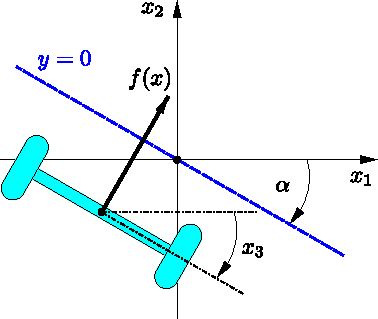
\includegraphics[width=0.5\textwidth]{Roboter_rel_Grad_mod}
\par\end{centering}
\caption{Roboter mit einem nicht überall wohldefinierten relativen Grad\label{fig:Roboter-rel-grad-gerade}}
\end{figure}

Ist die Bedingung~\ref{enu:rel-deg1} aus Definition~\ref{def:relativer-Grad-SISO}
für alle $k\in\NN$ erfüllt, dann definieren etliche Autoren einen
relativen Grad $r=\infty$, z.\,B.~\cite[Def.~{6.177}]{kwatny2000}.
Dieser Fall ist so zu verstehen, dass sich der Ausgang~$y$ in keiner
Weise durch den Eingang~$u$ beeinflussen lässt, also im System keine
,,interne`` Verbindung zwischen Eingang und Ausgang besteht. Das
trifft beispielsweise auf ein autonomes System $\dot{x}=f(x)$ zu.
Zusätzlich wird im nächsten Beispiel (wieder) der Spezialfall eines
linearen Systems behandelt. 
\begin{example}
\label{exa:Lineares-System-r-infty}Das lineare System~(\ref{eq:rel-grad-lineares-system})
aus Anmerkung~\ref{rem:rel-grad-Markovparameter} liege in einer
\emph{Kalman-Zerlegung}\index{Kalman-Zerlegung} 
\begin{eqnarray*}
\left(\begin{array}{c}
\dot{x}_{1}\\
\dot{x}_{2}\\
\dot{x}_{3}\\
\dot{x}_{4}
\end{array}\right) & = & \left(\begin{array}{cccc}
A_{11} & A_{12} & A_{13} & A_{14}\\
0 & A_{22} & 0 & A_{24}\\
0 & 0 & A_{33} & A_{34}\\
0 & 0 & 0 & A_{44}
\end{array}\right)\left(\begin{array}{c}
x_{1}\\
x_{2}\\
x_{3}\\
x_{3}
\end{array}\right)+\left(\begin{array}{c}
b_{1}\\
b_{2}\\
0\\
0
\end{array}\right)u\\
y & = & \left(\begin{array}{cccc}
0 & c_{2}^{T} & 0 & c_{4}^{T}\end{array}\right)x
\end{eqnarray*}
mit geeigneten Matrizen~$A_{11},A_{12},\ldots,A_{44}$ und passenden
Vektoren $b_{1},b_{2,}c_{2},c_{4}$ vor~\cite{lunze-rt2}. Dabei
sind das erste und zweite Teilsystem steuerbar sowie das zweite und
vierte Teilsystem beobachtbar. Das Eingangs-Ausgangs-Verhalten, welches
sich beispielsweise durch die Übertragungsfunktion beschreiben lässt,
hängt nur vom zweiten Teilsystem, das sowohl steuer- als auch beobachtbar
ist, ab~\cite{kalman1962canonical,lunze-rt2}. Das ist auch anhand
der gemischten Lie-Ableitungen bzw. der Markovparameter\index{Markovparameter}
zu erkennen: 
\[
L_{g}L_{f}^{k}h(x)=c^{T}A^{k}b=c_{2}^{T}A_{22}^{k}b_{2}.
\]
Die gemischte Lie-Ableitung des linearen Systems nimmt nur dann einen
von Null verschiedenen Wert an, wenn es ein gleichzeitig steuer- als
auch beobachtbares Teilsystem gibt. Andernfalls würde man im o.\,g.
Sinne $r=\infty$ erhalten.

\end{example}
\medskip{}

Das allgemeine Vorgehen beim Reglerentwurf für ein System~(\ref{eq:Ausgangssystem-fuer-BINF})
mit relativem Grad~$r$ lässt sich auf Basis von Gl.~(\ref{eq:rg-yrdot})
beschreiben. Der Reglerentwurf erfolgt in zwei Schritten:
\begin{enumerate}
\item Linearisierung durch Rückführung,
\item Stabilisierung des linearisierten Systems.
\end{enumerate}
Im ersten Schritt setzt man die rechte Seite von Gl.~(\ref{eq:rg-yrdot})
einer neuen Systemgröße~$v$ gleich, d.\,h. 
\begin{equation}
L_{f}^{r}h(x)+L_{g}L_{f}^{r-1}h(x)u\stackrel{!}{=}v,\label{eq:regler1-linearisierung-forderung}
\end{equation}
so kann man die Gleichung wegen $L_{g}L_{f}^{r-1}h(p)\neq0$ in einer
Umgebung von~$p$ nach~$u$ umstellen: 
\begin{equation}
u=\frac{1}{L_{g}L_{f}^{r-1}h(x)}\left(v-L_{f}^{r}h(x)\right).\label{eq:regler1-linearisierung}
\end{equation}
Die Systemgröße~$v$ lässt sich als neuer (virtueller) Eingang interpretieren.
Gl.~(\ref{eq:regler1-linearisierung}) beschreibt dann eine Zustandsrückführung
(siehe Abb.~\ref{fig:linearisierende-Zustandsrueckfuehrung}), mit
der Gleichung~(\ref{eq:rg-yrdot}) die Form einer Integratorkette
annimmt: 
\begin{equation}
y^{(r)}=v.\label{eq:regler-integratorkette}
\end{equation}
Durch die Rückführung~(\ref{eq:regler1-linearisierung}) werden die
in Gl.~(\ref{eq:rg-yrdot}) auftretenden Nichtlinearitäten kompensiert,
so dass man das lineare System~(\ref{eq:regler-integratorkette})
und damit ein lineares Eingangs-Ausgangs-Verhalten erhält. Man spricht
daher von einer \emph{Eingangs-Ausgangs-Linearisierung}. Die Rückführung~(\ref{eq:regler1-linearisierung})
nennt man auch \emph{linearisierende Rückführung}.

\begin{figure}
\begin{centering}
\resizebox{0.99\textwidth}{!}{\input{linearisierende-rueckfuehrung.pdftex_t}}
\par\end{centering}
\caption{Linearisierende Zustandsrückführung~(\ref{eq:regler1-linearisierung})\label{fig:linearisierende-Zustandsrueckfuehrung}}
\end{figure}

\begin{remark}
\label{rem:Hirschorn-Inverse}Das System~(\ref{eq:Ausgangssystem-fuer-BINF})
liefert das Ausgangssignal~$y$ als Antwort auf die Erregung durch
das Eingangssignal~$u$. Gibt man umgekehrt einen gewünschten Verlauf
des Ausgangssignals in Form einer $r$-mal stetig differenzierbaren
Funktion~$y$ vor, so kann man bei einem bekannten Verlauf des Zustands~$x$
durch Einsetzen von~(\ref{eq:regler-integratorkette}) in~(\ref{eq:regler1-linearisierung})
den zugehörigen Verlauf des Eingangssignals~$u$ ermitteln: 
\begin{equation}
u=\frac{1}{L_{g}L_{f}^{r-1}h(x)}\left(y^{(r)}-L_{f}^{r}h(x)\right).\label{eq:hirschorn-inverse-SISO}
\end{equation}
Mit Gl.~(\ref{eq:hirschorn-inverse-SISO}) wird (bei konsistenten
Anfangswerten) die Systemdynamik von~(\ref{eq:Ausgangssystem-fuer-BINF})
invertiert. Bei genauerer Betrachtung handelt es sich bei~(\ref{eq:hirschorn-inverse-SISO})
um eine \emph{Rechtsinverse}\index{Rechtsinverse} des Systems~(\ref{eq:Ausgangssystem-fuer-BINF}),
vgl. Abb.~\ref{fig:rechtsinverse-hirschon}. Die Inverse~(\ref{eq:hirschorn-inverse-SISO})
bzw. Gl.~(\ref{eq:regler1-linearisierung}) nennt man auch \emph{Hirschorn-Inverse}\index{Hirschorn-Inverse}~\cite{hirschorn1979,daoutidis1991,henson1997chap3}.
\end{remark}
\begin{figure}
\begin{centering}
\resizebox{0.99\textwidth}{!}{\input{hirschorn-inverse.pdftex_t}}
\par\end{centering}
\caption{Rechtsinverse~(\ref{eq:hirschorn-inverse-SISO}) des Systems~(\ref{eq:Ausgangssystem-fuer-BINF})\label{fig:rechtsinverse-hirschon}}
\end{figure}

Das durch Gl.~(\ref{eq:regler-integratorkette}) beschriebene Übertragungsglied
ist linear, aber instabil~\cite{reinschke2014buch}. Die zusätzliche
Rückführung 
\begin{equation}
v=-\sum_{k=0}^{r-1}a_{k}y^{(k)}\label{eq:regler2-stabilisierung}
\end{equation}
führt auf die lineare zeitinvariante Differentialgleichung 
\begin{equation}
y^{(r)}+a_{r-1}y^{(r-1)}+\cdots+a_{1}\dot{y}+a_{0}y=0.\label{eq:lineare-dgl-ordnung-r}
\end{equation}
Die Koeffizienten $a_{0},\ldots,a_{r-1}\in\R$ kann man so wählen,
dass alle Lösungen der zugehörigen charakteristischen Gleichung 
\begin{equation}
s^{r}+a_{r-1}s^{r-1}+\cdots+a_{1}s+a_{0}=0\label{eq:rg-gl-char-gleichung}
\end{equation}
negativen Realteil aufweisen. Ein solches charakteristisches Polynom
nennt man \emph{stabiles Polynom} oder \emph{Hurwitz-Polynom}\index{Hurwitz-Polynom}.
Dazu gibt man $r$ Nullstellen $s_{1},\ldots,s_{r}$ mit negativem
Realteil vor, wobei die Nullstellen reell sind oder in konjugiert
komplexen Paaren auftreten. Die Koeffizienten $a_{0},\ldots,a_{r-1}$
ergeben sich aus einem Koeffizientenvergleich: 
\[
(s-s_{1})\cdots(s-s_{r})\stackrel{!}{=}s^{r}+a_{r-1}s^{r-1}+\cdots+a_{1}s+a_{0}.
\]
Die Rückführung~(\ref{eq:regler2-stabilisierung}) stabilisiert in
diesem Fall das System und wird daher auch \emph{stabilisierende Rückführung}
genannt.

Die beiden Entwurfsschritte lassen sich einerseits zusammenfassen,
andererseits kann man Gl.~(\ref{eq:regler2-stabilisierung}) auch
über den Zustand~$x$ ausdrücken. Die Kombination von Gln.~(\ref{eq:regler1-linearisierung})
und~(\ref{eq:regler2-stabilisierung}) in Verbindung mit $y^{(k)}=L_{f}^{k}h(x)$
für $k=0,\ldots,r-1$ liefert die Zustandsrückführung 
\begin{equation}
u=-\frac{1}{L_{g}L_{f}^{r-1}h(x)}\sum_{k=0}^{r}a_{k}L_{f}^{k}h(x)\quad\text{mit}\quad a_{r}:=1.\label{eq:regler3-linearisierung-stabilisierung}
\end{equation}

Die Rückführung~(\ref{eq:regler3-linearisierung-stabilisierung})
stabilisiert die Ruhelage $y=0$ der Differentialgleichung~(\ref{eq:lineare-dgl-ordnung-r}).
Möchte man stattdessen für die Regelgröße~$y$ einen gewünschten
Sollwert vorgeben, so erweitert man die stabilisieriende Rückführung~(\ref{eq:regler2-stabilisierung})
um die Führungsgröße~$w$ zu 
\begin{equation}
v=a_{0}w-\sum_{k=0}^{r-1}a_{k}y^{(k)}.\label{eq:regler4-linearisierung-stabilisierung-sollwert-y}
\end{equation}
Ersetzt man die Zeitableitungen des Ausgangs durch die entsprechenden
Lie-Ableitungen, so lässt sich das Regelgesetz~(\ref{eq:regler4-linearisierung-stabilisierung-sollwert-y})
analog zu~(\ref{eq:regler3-linearisierung-stabilisierung}) als Zustandsrückführung
\begin{equation}
u=\frac{1}{L_{g}L_{f}^{r-1}h(x)}\left(a_{0}w-\sum_{k=0}^{r}a_{k}L_{f}^{k}h(x)\right)\label{eq:regler4-linearisierung-stabilisierung-sollwert-x}
\end{equation}
angeben. Mit der Rückführung~(\ref{eq:regler4-linearisierung-stabilisierung-sollwert-y})
bzw.~(\ref{eq:regler4-linearisierung-stabilisierung-sollwert-x})
erhält man die lineare Differentialgleichung 
\begin{equation}
y^{(r)}+a_{r-1}y^{(r-1)}+\cdots+a_{1}\dot{y}+a_{0}y=a_{0}w,\label{eq:lineare-dgl-ordnung-r-mit-w}
\end{equation}
siehe Abb.~\ref{fig:regelungsnormalform-lin-stab-w}. Der Faktor
vor der Führungsgröße~$w$ wurde so gewählt, dass bei konstantem~$w$
die Differentialgleichung~(\ref{eq:lineare-dgl-ordnung-r-mit-w})
die Ruhelage $y=w$ besitzt. Der gewünschte Sollwert~$w$ stellt
sich damit am Ausgang (asymptotisch) ein. Der Faktor $a_{0}$ agiert
in diesem Zusammenhang als (statisches) Vorfilter zur Sicherung des
jeweils gegebenen Sollwertes (siehe~\cite[Abschnitt~{4.4.2}]{lunze-rt2}).
Zwischen der Führungsgröße~$w$ und der Regel- bzw. Ausgangs\-größe~$y$
wirkt im Frequenzbereich (also zwischen den Laplace-Transformierten
$W$ und $Y$ der Signale~$w$ und~$y$) die Übertragungsfunktion
\begin{equation}
G_{W}^{Y}(s)=\frac{Y(s)}{W(s)}=\frac{a_{0}}{s^{r}+a_{r-1}s^{r-1}+\cdots+a_{1}s+a_{0}}.\label{eq:UF-WY}
\end{equation}
Die Stabilität dieses Übertragungsgliedes lässt sich durch die Wahl
der Koeffizienten $a_{0},\ldots,a_{n-1}$ sicherstellen. 

\begin{figure}
\begin{centering}
\resizebox{0.85\textwidth}{!}{\input{regelungsnormalform-lin-stab-w.pdftex_t}}
\par\end{centering}
\caption{Stabilisiertes Regelungssystem~(\ref{eq:lineare-dgl-ordnung-r-mit-w})\label{fig:regelungsnormalform-lin-stab-w}}
\end{figure}

\begin{example}
\label{exa:Roboter-geregelt1}Man betrachte den mobilen Roboter aus
Beispiel~\ref{exa:Roboter-rel-grad}. Für den Ausgang~(\ref{eq:roboter-rg-ausgang})
setzen wir $c_{1}=1$ und $c_{2}=0$. Der Ausgang $y=h(x)=x_{1}$
gibt in diesem Fall die $x_{1}$-Position des Roboters an. Die gemischte
Lie-Ableitung besitzt dann die Form $L_{g}L_{f}h(x)=\cos x_{3}$,
so dass der relative Grad $r=2$ für $x_{3}\notin\{\pi/2+k\pi,\,k\in\Z\}$
wohldefiniert ist. Zu entwerfen ist ein Regelgesetz, welches den Roboter
auf eine durch die Führungsgröße~$w$ vorgegebene $x_{1}$-Position
führt und diese Lage stabilisert. Aus Gl.~(\ref{eq:regler4-linearisierung-stabilisierung-sollwert-x})
ergibt sich die nichtlineare Zustandsrückführung 
\begin{eqnarray*}
u & = & \frac{1}{L_{g}L_{f}h(x)}\left(a_{0}\left(w-h(x)\right)-a_{1}L_{f}h(x)-L_{f}^{2}h(x)\right)\\
 & = & \frac{1}{\cos x_{3}}\left(a_{0}(w-x_{1})-a_{1}\sin x_{3}\right)
\end{eqnarray*}
mit den Koeffizienten $a_{0}$ und $a_{1}$. Für die Führungsübertragungsfunktion
geben wir eine doppelte Polstelle bei $s_{1,2}=-1$ vor, so dass man
aus $(s+1)^{2}=s^{2}+2s+1$ für die charakteristische Gleichung~(\ref{eq:rg-gl-char-gleichung})
die Koeffizienten $a_{0}=1$ und $a_{1}=2$ abliest. Abb.~\ref{fig:Roboter-geregelt1}
zeigt die Simulationsergebnisse des geregelten Robotermodells für
die Anfangswerte $x_{1}(0)=2$, $x_{2}(0)=1$, $x_{3}(0)=\pi/4$ ($\widehat{=}\,45\text{°}$)
und die Führungsgröße $w=1$. Die Konvergenz $y(t)=x_{1}(t)\to w=1$
für $t\to\infty$ ist visuell zu erkennen. Allerdings strebt der Roboter
nicht gegen eine Ruhelage, da er seine Fahrt (wegen der Annahme einer
konstanten Geschwindigkeit) parallel zur $x_{2}$-Achse fortsetzt.
\end{example}
\begin{figure}
\begin{centering}
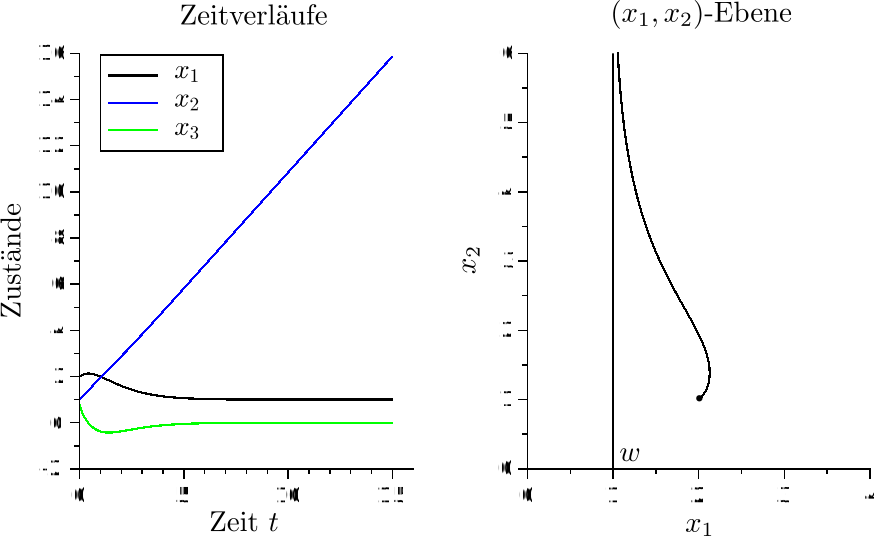
\includegraphics[width=0.85\textwidth]{robot_lin}
\par\end{centering}
\caption{Trajektorien des geregelten mobiler Robotermodells aus Beispiel~\ref{exa:Roboter-geregelt1}\label{fig:Roboter-geregelt1}}
\end{figure}

Den bisherigen Stabilitätsüberlegungen lagen die linearen Differentialgleichungen~(\ref{eq:lineare-dgl-ordnung-r})
bzw.~(\ref{eq:lineare-dgl-ordnung-r-mit-w}) zugrunde. Wenn der relative
Grad kleiner ist als die System\-ordnung, also für $r<n$, erfassen
diese Gleichungen nicht die komplette System\-dynamik. Daher spricht
man bei der Eingangs-Ausgangs-Linearisierung auch von einer \emph{partiellen
Linearisierung}.\index{partielle Linearisierung}\index{Linearisierung!partielle}
Die Betrachtung der gesamten System\-dynamik im Zustandsraum erfolgt
in Abschnitt~\ref{subsec:Byrnes-Isidori-Normalform}. Bei $r=n$
erzielt man eine vollständige Linearisierung, die sog. \emph{Eingangs-Zustands-Linearisierung},
die in Abschnitt~\ref{sec:Exakte-Eingangs-Zustands-Linearisierung}
behandelt wird.

Bei einer partiellen Linearisierung erhält man gerade bei mechanischen
Systemen oft deutlich einfache Differentialgleichungen, so dass dieser
Zugang auch für andere (z.\,B. energiebasierte) Regelungsansätze
hilfreich ist~\cite{spong1996}.

\begin{example}
\label{exa:Wagen-Pendel-partielle-Linearisierung}Das in Abschnitt~\ref{subsec:Wagen-mit-Pendel}
vorgestellte Wagen-Pendel-System wird durch die nicht ganz einfachen
Zustandsgleichungen
\begin{equation}
\begin{array}{lcl}
\dot{x}_{1} & = & x_{2}\\
\dot{x}_{2} & = & \frac{m_{2}\ell^{2}x_{4}^{2}\sin x_{3}-d_{1}\ell x_{2}+\cos x_{3}\left(m_{2}g\ell\sin x_{3}+d_{2}x_{4}\right)+\ell u}{\ell\left(m_{1}+m_{2}\sin^{2}x_{3}\right)}\\
\dot{x}_{3} & = & x_{4}\\
\dot{x}_{4} & = & \frac{-\left(m_{1}+m_{2}\right)\left(m_{2}g\ell\sin x_{3}+d_{2}x_{4}\right)-\cos x_{3}\left(\ell^{2}m_{2}^{2}x_{4}^{2}\sin x_{3}-d_{1}\ell m_{2}x_{2}\right)-\ell m_{2}u\cos x_{3}}{\ell^{2}m_{2}\left(m_{1}+m_{2}\sin^{2}x_{3}\right)}
\end{array}\label{eq:wagen-pendel-regler-grundlagen}
\end{equation}
beschrieben. Verwendet man als Ausgang die Position des Wagens, so
tritt der Eingang~$u$ erst in der zweiten Zeitableitung auf:
\begin{equation}
\begin{array}{lclclcl}
y & = & x_{1}\\
\dot{y} & = & \dot{x}_{1} & = & x_{2}\\
\ddot{y} & = & \dot{x}_{2} & = & \frac{m_{2}\ell^{2}x_{4}^{2}\sin x_{3}-d_{1}\ell x_{2}+\cos x_{3}\left(m_{2}g\ell\sin x_{3}+d_{2}x_{4}\right)+\ell u}{\ell\left(m_{1}+m_{2}\sin^{2}x_{3}\right)} & \stackrel{!}{=} & v.
\end{array}\label{eq:wagen-pendel-zeitableitungen}
\end{equation}
Eine partielle Linearisierung erzielt man, indem man die letzte Gleichung
nach dem Eingang~$u$ umstellt: 
\begin{equation}
u=v\left(m_{1}+m_{2}\sin^{2}x_{3}\right)-m_{2}\sin x_{3}\left(\ell x_{4}^{2}+g\cos x_{3}\right)+d_{1}x_{2}-\frac{d_{2}}{\ell}x_{4}\cos x_{3}.\label{eq:wagen-pendel-u-partiell-lin}
\end{equation}
Das entspricht formal dem Übergang von~(\ref{eq:regler1-linearisierung-forderung})
zu~(\ref{eq:regler1-linearisierung}). Setzt man~(\ref{eq:wagen-pendel-u-partiell-lin})
in Gl.~(\ref{eq:wagen-pendel-regler-grundlagen}) ein, so vereinfacht
sich nicht nur die zweite, sondern auch die vierte Gleichung von~(\ref{eq:wagen-pendel-regler-grundlagen}).
Insgesamt erhält man das folgende partiell linearisierte System\foreignlanguage{english}{:}
\begin{equation}
\begin{array}{lcl}
\dot{x}_{1} & = & x_{2}\\
\dot{x}_{2} & = & v\\
\dot{x}_{3} & = & x_{4}\\
\dot{x}_{4} & = & -\frac{d_{2}}{\ell^{2}m_{2}}x_{4}-\frac{g}{\ell}\sin x_{3}-\frac{1}{\ell}v\cos x_{3}\\
y & = & x_{1}.
\end{array}\label{eq:wagen-pendel-kollokiert-linearisiert}
\end{equation}
\end{example}

Wenn bei der Eingangs-Ausgangs-Linearisierung eines mechanischen Systems
Eingang und Ausgang die gleiche Konfigurationskoordinate (bzw. das
gleiche Gelenk) betreffen, dann spricht man von einer \emph{kollokierten}\index{Linearisierung!kollokierte},
andernfalls von einer \emph{nicht-kollokierten} partiellen Linearisierung~\cite{spong1994,spong1998}.
In Beispiel~\ref{exa:Wagen-Pendel-partielle-Linearisierung} wird
bezüglich der Koordinate~$q_{1}$ eine kollokierte Linearisierung
vorgenommen. Hätte man stattdessen $q_{2}=x_{3}$ als Ausgang verwendet,
so würde eine nicht-kollokierte Linearisierung vorliegen.

\subsection{Byrnes-Isidori-Normalform\label{subsec:Byrnes-Isidori-Normalform}}

Dieser Abschnitt befasst sich mit der Transformation eines gegebenen
Systems~(\ref{eq:Ausgangssystem-fuer-BINF}) in eine Form, die sowohl
zur Untersuchung des Eingangs-Ausgangs-Verhaltens als auch für die
Beschreibung des geregelten Systems sinnvoll ist. Bei der herzuleitenden
Transformation kommt dem relativen Grad eine besondere Bedeutung zu.
In diesem Abschnitt gehen wir davon aus, dass das System~(\ref{eq:Ausgangssystem-fuer-BINF})
im Punkt $p\in\mathcal{M}$ den wohldefinierten relativen Grad~$r$
besitzt. 

Bei den in der Definition des relativen Grades auftretenden gemischten
Lie-Ableitungen $L_{g}L_{f}^{i}h$ wird von dem Skalarfeld~$h$ eine
Lie-Ableitung der Ordnung $i+1$ gebildet, nämlich $i$ mal in Richtung
des Vektorfeldes~$f$ und einmal in Richtung des Vektorfeldes~$g$.
Das folgende Lemma besagt, dass man die Ableitungsordnung für das
Skalarfeldes~$h$ reduzieren kann, wenn man statt dessen entsprechende
Lie-Ableitungen des Vektorfeldes~$g$ (also Lie-Klammern) bildet.
Diese Hilfsaussage wird auch für die Eingangs-Zustands-Linearisierung
benötigt (siehe Abschnitt~\ref{sec:Exakte-Eingangs-Zustands-Linearisierung}).
\begin{lemma}
\label{lem:Skalarprod-dLf-ad}In einer Umgebung von~$p$ gilt 
\begin{equation}
\left\langle \d L_{f}^{j}h,\ad_{-f}^{i}g\right\rangle =\left\{ \begin{array}{ccccc}
0 & \mbox{für} & i+j & < & r-1,\\
L_{g}L_{f}^{r-1}h & \mbox{für} & i+j & = & r-1.
\end{array}\right.\label{eq:SP-dLfj,adi}
\end{equation}
\end{lemma}
\begin{svmultproof2}
Wir beweisen die Aussage mit Induktion über~$i$ bei festem~$j$.
Induktionsanfang ($i=0$): Es gilt 
\[
\left\langle \d L_{f}^{j}h,g\right\rangle =L_{g}L_{f}^{j}h=\left\{ \begin{array}{ccccc}
0 & \mbox{für} & j & < & r-1,\\
L_{g}L_{f}^{r-1}h & \mbox{für} & j & = & r-1,
\end{array}\right.
\]
da das System~(\ref{eq:Ausgangssystem-fuer-BINF}) den relativen
Grad~$r$ besitzt. 

Gl.~(\ref{eq:SP-dLfj,adi}) gelte für $i=0,\ldots,k-1$ (Induktionsannahme).
Der Induktionsschritt für $k+j\leq r-1$ liefert
\[
\begin{array}{ccl}
\left\langle \d L_{f}^{j}h,\ad_{-f}^{k}g\right\rangle  & = & \d L_{f}^{j}h\cdot\ad_{-f}^{k}g\\
 & = & L_{\ad_{-f}^{k}g}L_{f}^{j}h\\
 & = & L_{[-f,\ad_{-f}^{k-1}g]}L_{f}^{j}h\\
 & = & -\underbrace{L_{f}L_{\ad_{-f}^{k-1}g}L_{f}^{j}h}_{{\displaystyle =0}}+L_{\ad_{-f}^{k}g}L_{f}L_{f}^{j}h,
\end{array}
\]
wobei der erste Summand nach Induktionsannahme Null ist. Damit gilt
weiter 
\[
\begin{array}{lcl}
\left\langle \d L_{f}^{j}h,\ad_{-f}^{k}g\right\rangle  & = & L_{\ad_{-f}^{k}g}L_{f}L_{f}^{j}h\\
 & = & L_{\ad_{-f}^{k}g}L_{f}^{j+1}h\\
 & = & \left\langle \d L_{f}^{j+1}h,\ad_{-f}^{k-1}g\right\rangle .
\end{array}
\]
An dieser Stelle bietet sich eine Fallunterscheidung an:

\begin{enumerate}
\item $k+j<r-1$. Das impliziert $(k-1)+(j+1)<r$, d.\,h. nach Induktionsannahme
gilt 
\[
\left\langle \d L_{f}^{j}h,\ad_{-f}^{k}g\right\rangle =\left\langle \d L_{f}^{j+1}h,\ad_{-f}^{k-1}g\right\rangle =0.
\]
\item $k+j=r-1$. Die Induktionsannahme liefert 
\begin{eqnarray*}
\left\langle \d L_{f}^{j}h,\ad_{-f}^{k}g\right\rangle  & = & \left\langle \d L_{f}^{j+1}h,\ad_{-f}^{k-1}g\right\rangle \\
 & \vdots\\
 & = & \left\langle \d L_{f}^{r-1}h,\ad_{-f}^{0}g\right\rangle \\
 & = & \left\langle \d L_{f}^{r-1}h,g\right\rangle \\
 & = & L_{g}L_{f}^{r-1}h.
\end{eqnarray*}
\end{enumerate}
Damit ist Lemma~\ref{lem:Skalarprod-dLf-ad} bewiesen.
\end{svmultproof2}

Die nächste Hilfsaussage bildet die Grundlage für die Konstruktion
eines $r$-dimensionalen ersten Teilsystems.
\begin{lemma}
\label{lem:Lin-Unabh-Kovektoren}Die Kovektoren 
\[
\d h(p),\,\d L_{f}h(p),\,\ldots,\,\d L_{f}^{r-1}h(p)
\]
sind linear unabhängig.
\end{lemma}
\begin{svmultproof2}
Wegen Lemma~\ref{lem:Skalarprod-dLf-ad} gilt
\begin{equation}
\begin{array}{l}
\left(\begin{array}{c}
\d h(p)\\
\d L_{f}h(p)\\
\vdots\\
\d L_{f}^{r-1}h(p)
\end{array}\right)\left(g(p),\ad_{-f}g(p),\ldots,\ad_{-f}^{r-1}g(p)\right)=\\
=\left(\begin{array}{cccc}
0 & \cdots & 0 & \langle\d h,\ad_{f}^{r-1}g\rangle(p)\\
\vdots & \qdots &  & *\\
0 &  & \qdots & \vdots\\
\langle\d L_{f}^{r-1}h,g\rangle(p) & * & \cdots & *
\end{array}\right)\\
=\left(\begin{array}{cccc}
0 & \cdots & 0 & L_{g}L_{f}^{r-1}h(p)\\
\vdots & \qdots &  & *\\
0 &  & \qdots & \vdots\\
L_{g}L_{f}^{r-1}h(p) & * & \cdots & *
\end{array}\right).
\end{array}\label{eq:Lin-Unabh-Kov-Beweis1}
\end{equation}
Wegen $L_{g}L_{f}^{r-1}h(p)\neq0$ ist die rechte Seite regulär mit
Rang~$r$. Daher müssen die Zeilen der Matrix 
\begin{equation}
\left(\begin{array}{c}
\d h(p)\\
\vdots\\
\d L_{f}^{r-1}h(p)
\end{array}\right)\label{eq:Lin-Unabh-Kov-Beweis2}
\end{equation}
linear unabhängig sein. 
\end{svmultproof2}

\begin{remark}
\label{rem:relativer-Grad-Systemordnung}Aus Lemma~\ref{lem:Lin-Unabh-Kovektoren}
folgt zusätzlich, dass der relative Grad~$r$ nicht die Systemdimension~$n$
übersteigen kann, also mit einem wohldefinierten relativen Grad~$r$
auch $r\leq n$ gilt: Angenommen, die Bedingungen aus Def.~\ref{def:relativer-Grad-SISO}
seien für eine natürliche Zahl $r>n$ erfüllt. Die rechte Seite von
Gl.~(\ref{eq:Lin-Unabh-Kov-Beweis1}) müsste dann den Rang $r>n$
haben. Das steht im Widerspruch zu der Aussage, dass die auf der linken
Seite von Gl.~(\ref{eq:Lin-Unabh-Kov-Beweis1}) als Faktor auftretende
$r\times n$-Matrix~(\ref{eq:Lin-Unabh-Kov-Beweis2}) höchsten den
Rang~$n$ besitzen kann.
\end{remark}

Auf Basis von Lemma~\ref{lem:Lin-Unabh-Kovektoren} lassen sich die
ersten $r$ Koordinaten einer neuen Zustandsraumdarstellung des Systems~(\ref{eq:Ausgangssystem-fuer-BINF})
angeben. Durch eine standardmäßige Basisergänzung um $n-r$ weitere
Koordinaten wird man auf die nachfolgend angegebene Zwischenform geführt~\cite{chen1996,devasia1996}:
\begin{theorem}
\label{thm:EA-Form}Wir setzen 
\begin{equation}
\begin{array}{lcl}
\phi_{1}(x) & = & h(x)\\
\phi_{2}(x) & = & L_{f}h(x)\\
 & \vdots\\
\phi_{r}(x) & = & L_{f}^{r-1}h(x).
\end{array}\label{eq:Phi1}
\end{equation}
Für $r<n$ gibt es $n-r$ weitere glatte Funktionen $\phi_{r+1},\ldots,\phi_{n}$,
so dass 
\begin{equation}
z=\Phi(x)=\left(\begin{array}{c}
\phi_{1}(x)\\
\vdots\\
\phi_{n}(x)
\end{array}\right)\label{eq:Phi}
\end{equation}
in der Umgebung des Punktes~$p$ ein lokaler Diffeomorphismus ist,
der das System~(\ref{eq:Ausgangssystem-fuer-BINF}) in die \emph{Eingangs-Ausgangs-Normalform}\index{Eingangs-Ausgangs-Normalform}\index{Normalform!Eingangs-Ausgangs-}\footnote{Unter einer \emph{Normalform} wird in diesem Buch die Darstellung
eines mathematischen Objektes mit vorgegebenen Eigenschaften verstanden.
Im Unterschied zu anderen Autoren wird hier keine Eindeutigkeit dieser
Darstellung gefordert.}
\begin{equation}
\begin{array}{lcl}
\dot{z}_{1} & = & z_{2}\\
 & \vdots\\
\dot{z}_{r-1} & = & z_{r}\\
\dot{z}_{r} & = & \alpha(z)+\beta(z)u\\
\dot{z}_{r+1} & = & q_{1}(z)+d_{1}(z)u\\
 & \vdots\\
\dot{z}_{n} & = & q_{n-r}(z)+d_{n-r}(z)u\\
y & = & z_{1}
\end{array}\label{eq:EA-Form-komponentenweise}
\end{equation}
überführt.
\end{theorem}
\begin{svmultproof2}
Nach Lemma~\ref{lem:Lin-Unabh-Kovektoren} sind die Zeilenvektoren
$\d h(p),\ldots,\d L_{f}^{r-1}h(p)\in(\R^{n})^{*}$ linear unabhängig.
Diese Kovektoren spannen einen $r$-dimensionalen Unterraum~$\mathbb{U}$
im Dualraum~$(\R^{n})^{*}$ auf. Der zugehörige \index{Annihilatorraum}Annihilatorraum~$\mathbb{U}^{\perp}$
ist ein $(n-r)$-dimensionaler Unterraum des~$\R^{n}$ und habe die
Basis $b_{1},\ldots,b_{n-r}\in\R^{n}$, d.\,h. $\mathbb{U}^{\perp}=\spann\{b_{1},\ldots,b_{n-r}\}$.
Die Funktionen~(\ref{eq:Phi1}) ergänzen wir durch die linearen Funktionen
\begin{equation}
\begin{array}{rcl}
\phi_{r+1}(x) & = & b_{1}^{T}x,\\
 & \vdots\\
\phi_{n}(x) & = & b_{n-r}^{T}x.
\end{array}\label{eq:Phi2}
\end{equation}
 Die Jacobimatrix 
\[
\Phi^{\prime}(p)=\left(\begin{array}{c}
\D h(p)\\
\vdots\\
\D L_{f}^{r-1}h(p)\\
\hline b_{1}^{T}\\
\vdots\\
b_{n-r}^{T}
\end{array}\right)\in\R^{n\times n}
\]
der Abbildung~$\Phi$ ist im Punkt~$p$ aufgrund des Dimensionssatzes
regulär (vgl. Abschnitt~\ref{sec:Lineare-Algebra}). Nach dem Satz
über die Umkehrfunktion ist $z=\Phi(x)$ ein lokaler Diffeomorphismus.\footnote{Mit der linearen Unabhängigkeit der Gradienten $\d h(p),\ldots,\d L_{f}^{r-1}h(p)$
wäre die Existenz eines lokalen Diffeomorphismus bereits nach Korollar~\ref{cor:ergaenzung-einer-kodistribution-integrierbar}
gesichert. Das hier beschriebene Vorgehen ist jedoch in Hinblick auf
die Berechnung der Koordinatentransformation einfacher.} 

Nun ist zu zeigen, dass das transformierte System die Form~(\ref{eq:EA-Form-komponentenweise})
besitzt. Zunächst betrachten wir die Koordinaten $z_{i}=\phi_{i}(x)=L_{f}^{i-1}h(x)$
mit $i=1,\ldots,r$ des ersten Teilsystems von~(\ref{eq:EA-Form-komponentenweise}).
Für $i=1,\ldots,r-1$ gilt 
\begin{eqnarray*}
\dot{z}_{i} & = & \frac{\d}{\d t}\phi_{i}(x)\\
 & = & \d\phi_{i}(x)\cdot\dot{x}\\
 & = & \d L_{f}^{i-1}h(x)\cdot\left(f(x)+g(x)u\right)\\
 & = & L_{f}^{i}h(x)+\underbrace{L_{g}L_{f}^{i-1}h(x)}_{{\displaystyle \equiv0\mbox{ da }i<r}}u\\
 & = & \phi_{i+1}(x)\\
 & = & z_{i+1}.
\end{eqnarray*}
Bei $i=r$ gilt 
\begin{eqnarray*}
\dot{z}_{r} & = & \frac{\d}{\d t}\phi_{r}(x)\\
 & = & \d\phi_{r}(x)\cdot\dot{x}\\
 & = & \d L_{f}^{r-1}h(x)\cdot\left(f(x)+g(x)u\right)\\
 & = & L_{f}^{r}h(x)+\underbrace{L_{g}L_{f}^{r-1}h(x)}_{{\displaystyle \neq0}}u.
\end{eqnarray*}
Ein Vergleich mit Zeile~$r$ des Systems~(\ref{eq:EA-Form-komponentenweise})
liefert
\begin{equation}
\begin{array}{lcl}
\alpha(z) & = & \left.L_{f}^{r}h(x)\right|_{x=\Phi^{-1}(z)}\\
\beta(z) & = & \left.L_{g}L_{f}^{r-1}h(x)\right|_{x=\Phi^{-1}(z)}.
\end{array}\label{eq:alpha-beta-EA-NF}
\end{equation}

Anschließend betrachten wir die Koordinaten $z_{i}=\phi_{i}(x)$ mit
$i=r+1,\ldots,n$ des zweiten Teilsystems von~(\ref{eq:EA-Form-komponentenweise}).
Es gilt
\begin{eqnarray*}
\dot{z}_{i} & = & \frac{\d}{\d t}\phi_{i}(x)\\
 & = & \d\phi_{i}(x)\cdot\dot{x}\\
 & = & \d\phi_{i}(x)\cdot\left(f(x)+g(x)u\right)\\
 & = & L_{f}\phi_{i}(x)+L_{g}\phi_{i}(x)u.
\end{eqnarray*}
Die Funktionen $q_{1},\ldots,q_{n-r}$ und $d_{1},\ldots,d_{n-r}$
auf der rechten Seite der letzten $n-r$ Zeilen des Systems sind dementsprechend
durch
\[
\begin{array}{ccc}
q_{i}(z) & = & \left.L_{f}\phi_{r+i}(x)\right|_{x=\Phi^{-1}(z)}\\
d_{i}(z) & = & \left.L_{g}\phi_{r+i}(x)\right|_{x=\Phi^{-1}(z)}
\end{array}
\]
 für $i=1,\ldots,n-r$ definiert.
\end{svmultproof2}

\begin{remark}
Im Beweis wurde der von den Kovektoren $\d h(p),\ldots,\d L_{f}^{r-1}h(p)$
aufgespannte Unterraum $\mathbb{U}\subset(\R^{n})^{*}$ letztlich
durch sein orthogonales Komplement ergänzt. Alternativ ist auch die
Ergänzung durch eine geeignete Auswahl $\d x_{i_{1}},\ldots,\d x_{i_{n-r}}$
der kanonischen Basisvektoren möglich (Basis\-aus\-tausch\-satz
bzw. Aus\-tausch\-satz von Steinitz~\cite{kerner2007}), woraus
sich die zusätzlichen Funktionen $\phi_{r+1}(x)=x_{i_{1}},\ldots,\phi_{n}(x)=x_{i_{n-r}}$
ergeben. Bei diesem Zugang sind für das zweite Teilsystem keine neuen
Koordinaten festzulegen, sondern nur bestehende Koordinaten auszuwählen.
\end{remark}

Die im ersten Teilsystem der Eingangs-Ausgangs-Normalform~(\ref{eq:EA-Form-komponentenweise})
auftretenden Funktionen~$\alpha$ und~$\beta$ sind oft vergleichsweise
komplizierte Funktionen, die durch umfangreiche Ausdrücke beschrieben
werden. Da diese Nichtlinearitäten ohnehin kompensiert werden sollen
bietet es sich an, die Eingangs-Ausgangs-Linearisierung bereits \textit{vor}
der Berechnung der Normalform~(\ref{eq:EA-Form-komponentenweise})
durchzuführen. Nach einer solchen partiellen Linearisierung gilt $\alpha=0$
und $\beta=1$. 

\begin{example}
\label{exa:Wagen-Pendel-EA-NF}Man betrachte das Wagen-Pendel-System~(\ref{eq:wagen-pendel-regler-grundlagen})
aus Beispiel~\ref{exa:Wagen-Pendel-partielle-Linearisierung}. Die
partielle Linearisierung mit relativem Grad $r=2$ führt auf das deutlich
einfachere System~(\ref{eq:wagen-pendel-kollokiert-linearisiert}),
welches bereits in der Eingangs-Ausgangs-Normalform vorliegt. Dabei
wird das erste Teilsystem durch die Koordinaten $x_{1},x_{2}$ und
das zweite Teilsystem durch $x_{3},x_{4}$ beschrieben.
\end{example}

Mit der Eingangs-Ausgangs-Normalform zerfällt das System~(\ref{eq:Ausgangssystem-fuer-BINF})
in ein $r$-dimensionales erstes Teilsystem und ein $(n-r$)-dimensionales
zweites Teilsystem. Mit dem nächsten Lemma wird die Elimination des
Eingangs im zweiten Teilsystem ermöglicht~\cite[Prop.~{4.1.3}]{isidori3}.
\begin{lemma}
\label{lem:LgNull}Die ersten Koordinaten~(\ref{eq:Phi1}) können
durch zusätzliche Funktionen $\phi_{r+1},\ldots,\phi_{n}$ derart
ergänzt werden, dass die Abbildung~(\ref{eq:Phi}) im Punkt $p\in\mathcal{M}$
eine reguläre Jacobi\-matrix besitzt und außerdem 
\begin{equation}
L_{g}\phi_{i}(x)=0\quad\mbox{für}\quad i=r+1,\ldots,n\label{eq:Lg-phi}
\end{equation}
und alle~$x$ aus einer Umgebung von~$p$ gilt.
\end{lemma}

\begin{svmultproof2}
Aufgrund des wohldefinierten relativen Grades gilt $g(p)\neq0$. Dann
ist die Distribution $\Delta=\spann\{g\}$ regulär, und da sie eindimensional
ist auch involutiv: $[g,g]=0$. Der Satz von Frobenius (Satz~\ref{thm:Frobenius-lokal})
garantiert die Existenz von $n-1$ Skalarfeldern $\lambda_{1},\ldots,\lambda_{n-1}$
mit 
\begin{equation}
\Delta^{\perp}=\spann\{\d\lambda_{1},\ldots,\d\lambda_{n-1}\}\quad\text{und}\quad\dim(\Delta^{\perp})(p)=n-1.\label{eq:Annihil-n-1-fuer-BINF}
\end{equation}
Diese Skalarfelder erfüllen damit einerseits die Gleichung
\[
L_{g}\lambda_{i}(x)=0
\]
für $i=1,\ldots,n-1$ und alle~$x$ aus einer Umgebung von~$p$,
andererseits sind die Gradienten $\d\lambda_{i}$ im Punkt~$p$ linear
unabhängig (Dimensionsformel~(\ref{eq:dimensionssatz-distr-annihilator})
in Prop.~\ref{pro:Annihilator}). Wegen 
\[
\left\langle \d L_{f}^{k}h,g\right\rangle =L_{g}L_{f}^{k}h=0,\quad k=0,\ldots,r-2
\]
entsprechend Def.~\ref{def:relativer-Grad-SISO} sind bereits $r-1$
derartige Funktionen bekannt: $\lambda_{1}(x)=\phi_{1}(x)=h(x),\ldots,\lambda_{r-1}=\phi_{r-1}(x)=L_{f}^{r-2}h(x)$.
Die zugehörigen Gradienten sind zudem im Punkt~$p$ linear unabhängig
(Lemma~\ref{lem:Lin-Unabh-Kovektoren}). Damit existieren $(n-1)-(r-1)=n-r$
weitere (unabhängige) Funktionen $\phi_{r+1}(x)=\lambda_{r}(x),\ldots,\phi_{n}(x)=\lambda_{n-1}(x)$,
für welche Gl.~(\ref{eq:Annihil-n-1-fuer-BINF}) erfüllt ist. Außerdem
gilt aber auch 
\[
\left\langle \d L_{f}^{r-1}h,g\right\rangle =L_{g}L_{f}^{r-1}h(p)\neq0,
\]
so dass $\d L_{f}^{r-1}h$ nicht zum Annihiltor~$\Delta^{\perp}$
gehört. Damit gilt 
\[
\Delta^{\perp}(p)\oplus\spann\{\d L_{f}^{r-1}h(p)\}=(\R^{n})^{*},
\]
so dass mit $\phi_{r}(x)=L_{f}^{r-1}h(x)$ die Abbildung~$\Phi$
im Punkt~$p$ eine reguläre Jacobimatrix besitzt.
\end{svmultproof2}

Wählt man die Funktionen $\phi_{r+1},\ldots,\phi_{n}$ der Koordinatentransformation~(\ref{eq:Phi})
entsprechend Lemma~\ref{lem:LgNull}, dann geht die Eingangs-Ausgangs-Normalform
in die Byrnes-Isidori-Normalform über:
\begin{theorem}
\label{thm:Byrnes-Isidori-Normalform}Die in Lemma~\ref{lem:LgNull}
definierte Abbildung~$\Phi$ ist ein lokaler Diffeomorphismus, mit
dem System~(\ref{eq:Ausgangssystem-fuer-BINF}) in die \emph{Byrnes-Isidori-Normalform}\index{Normalform!Byrnes-Isidori-}\index{Byrnes-Isidori-Normalform}
\begin{equation}
\begin{array}{lcl}
\dot{z}_{1} & = & z_{2}\\
 & \vdots\\
\dot{z}_{r-1} & = & z_{r}\\
\dot{z}_{r} & = & \alpha(z)+\beta(z)u\\
\dot{z}_{r+1} & = & q_{1}(z)\\
 & \vdots\\
\dot{z}_{n} & = & q_{n-r}(z)\\
y & = & z_{1}
\end{array}\label{eq:BINF-Komponentenweise}
\end{equation}
überführt wird.
\end{theorem}
\begin{svmultproof2}
Bei wohldefiniertem relativen Grad~$r$ existiert nach Satz~\ref{thm:EA-Form}
die Eingangs-Ausgangs-Normalform~(\ref{eq:EA-Form-komponentenweise}).
Die ersten $r$ Koordinaten sind durch Gl.~(\ref{eq:Phi1}) gegeben.
Die zusätzlichen Koordinaten können entsprechend Gl.~(\ref{eq:Lg-phi})
gewählt werden (Lemma~\ref{lem:LgNull}). Für die Koordinaten $z_{i}=\phi_{i}(x)$
mit $i=r+1,\ldots,n$ des zweiten Teilsystems von~(\ref{eq:BINF-Komponentenweise})
gilt folglich
\begin{eqnarray*}
\dot{z}_{i} & = & \frac{\d}{\d t}\phi_{i}(x)\\
 & = & \d\phi_{i}(x)\cdot\dot{x}\\
 & = & \d\phi_{i}(x)\cdot\left(f(x)+g(x)u\right)\\
 & = & L_{f}\phi_{i}(x)+\underbrace{L_{g}\phi_{i}(x)}_{{\displaystyle \equiv\mbox{0}}}u\\
 & = & L_{f}\phi_{i}(x).
\end{eqnarray*}
Damit geht~(\ref{eq:EA-Form-komponentenweise}) in Gl.~(\ref{eq:BINF-Komponentenweise})
über, wobei das zweite Teilsystem nicht mehr direkt vom Eingang abhängt.
Die Funktionen $q_{1},\ldots,q_{n-r}$ auf der rechten Seite des zweiten
Teilsystems sind durch 
\[
q_{i}(z)=\left.L_{f}\phi_{r+i}(x)\right|_{x=\Phi^{-1}(z)}
\]
definiert.
\end{svmultproof2}

\begin{remark}
\label{rem:Berechnung-Byrnes-Isidori-NF}Für die Bestimmung der zusätzlichen
Funktionen $\phi_{r+1},\ldots,\phi_{n}$ kann man ausnutzen, dass
Lemma~\ref{lem:LgNull} mit dem Satz von Frobenius (Satz~\ref{thm:Frobenius-lokal})
bewiesen wurde, dessen Beweis konstruktiv mit Hilfe des Begradigungssatzes
(Satz~\ref{thm:simultane-begradigung-von-VF}) geführt wurde. Zur
Berechnung der gesuchten Funktionen ergänzt man das Eingangsvektorfeld
$g_{1}:=g$ um $n-1$ weitere (möglichst einfache) Vektorfelder $g_{2},\ldots,g_{n}$,
so dass alle Vektorfelder im Punkt~$p$ linear unabhängig sind. Dazu
kann man konstante Vektorfelder, insbesondere auch Einheitsvektorfelder
$\tfrac{\partial}{\partial x_{i}}$ verwenden. Die von diesen $n$
Vektorfeldern aufgespannte Distribution ist regulär und (da sie den
gesamten Raum aufspannt) involutiv. Wie in Gl.~(\ref{eq:S-flussverknuepfung})
des Beweises von Satz~\ref{thm:simultane-begradigung-von-VF} definiert
man über die Verkettung der Flüsse dieser Vektorfelder eine Abbildung\index{Fluss!Verkettung}
\begin{equation}
x=S(\tilde{z})=\varphi_{\tilde{z}_{1}}^{g_{1}}\circ\cdots\circ\varphi_{\tilde{z}_{n}}^{g_{n}}(p).\label{eq:flussverkettung-berechnung-BINF}
\end{equation}
Zu der Umkehrfunktion $\tilde{z}=T(x)$ betrachte man die Komponenten
$t_{2},\ldots,t_{n}$. Die zugehörigen Gradienten $\d t_{2},\ldots,\d t_{n}$
spannen in einer Umgebung des Punktes~$p$ den Annihilator von $\spann\{g\}$
auf (vgl. Beweis von Satz~\ref{thm:Frobenius-lokal}). Da die Gradienten
$\d h,\ldots,\d L_{f}^{r-2}h$ eine $r$-dimensionale Kodistribution
aufspannen, die im Annihilator enthalten ist, kann man von den Gradienten
$\d t_{2},\ldots,\d t_{n}$ genau $n-r$ Elemente zur Ergänzung der
Basis auswählen (Basis\-aus\-tausch\-satz bzw. Aus\-tausch\-satz
von Steinitz~\cite{kerner2007}).
\end{remark}

\begin{remark}
\label{rem:Berechnung-Byrnes-Isidori-NF-PDE}Formal stellt Gl.~(\ref{eq:Lg-phi})
eine \textit{partielle} Differentialgleichung dar, für die in Ergänzung
zu den bekannten Lösungen $h,L_{f}h,\ldots,L_{f}^{r-1}h$ (vgl. Punkt~\ref{enu:rel-deg1}
aus Def.~\ref{def:relativer-Grad-SISO}) noch $n-r$ weitere (unabhängige)
Lösungen $\phi_{r+1},\ldots,\phi_{n}$ gesucht sind. Grundsätzlich
bietet sich zur Lösung der partiellen Differentialgleichung~(\ref{eq:Lg-phi})
die Methode der Charakteristiken an~\cite{john1971}. Die symbolische
Lösung ist mit Computer-Algebra-Systemen nicht immer möglich~\cite{jager1991,jager95}. 
\end{remark}

Allerdings lassen sich in vielen Fällen die zusätzlichen Koordinaten
der Byrnes-Isidori-Normalform direkt angeben:

\begin{example}
\label{exa:Roboter-BI-NF}Man betrachte den mobilen Roboter aus Beispiel~\ref{exa:Roboter-rel-grad}
mit dem in Beispiel~\ref{exa:Roboter-geregelt1} verwendeten Ausgang
$y=x_{1}$. Der relative Grad $r=2$ ist für $x_{3}\notin\{\pi/2+k\pi,\,k\in\Z\}$
wohldefiniert. Die ersten $r$ Koordinaten der Byrnes-Isidori-Normalform
ergeben sich aus den Lie-Ableitungen
\begin{equation}
\begin{array}{lclcccl}
z_{1} & = & \phi_{1}(x) & = & h(x) & = & x_{1}\\
z_{2} & = & \phi_{2}(x) & = & L_{f}h(x) & = & \sin x_{3}.
\end{array}\label{eq:Roboter-BI-NF-hin1}
\end{equation}
Die dritte Koordinate muss von $x_{2}$ abhängen, andernfalls kann
die zur Koordinatentransformation gehörende Jacobimatrix nicht regulär
sein. Die lineare Funktion 
\begin{equation}
z_{3}=\phi_{3}(x)=x_{2}\label{eq:Roboter-BI-NF-hin2}
\end{equation}
erfüllt zudem noch die partielle Differentialgleichung~(\ref{eq:Lg-phi}).
Für $x_{3}\in(-\pi/2,+\pi/2)$ beschreiben die Gleichungen~(\ref{eq:Roboter-BI-NF-hin1})
und~(\ref{eq:Roboter-BI-NF-hin2}) einen Diffeomorphismus, dessen
Umkehrabbildung $z=\Phi^{-1}(x)$ durch 
\[
\begin{array}{lcl}
x_{1} & = & z_{1}\\
x_{2} & = & z_{3}\\
x_{3} & = & \arcsin z_{2}
\end{array}
\]
gegeben ist. Die Nichtlinearitäten~$\alpha$ und~$\beta$ des ersten
Teilsystems haben dann die Form 
\[
\alpha(z)=\left.L_{f}^{2}h(x)\right|_{x=\Phi^{-1}(z)}\equiv0
\]
und
\[
\beta(z)=\left.L_{g}L_{f}h(x)\right|_{x=\Phi^{-1}(z)}=\left.\cos x_{3}\right|_{x_{3}=\arcsin z_{2}}=\sqrt{1-z_{2}^{2}}\enspace.
\]
Für die Nichtlinearität des zweiten Teilsystems errechnet man 
\[
q_{1}(z)=\left.L_{f}\phi_{3}(x)\right|_{x=\Phi^{-1}(z)}=\left.\cos x_{3}\right|_{x_{3}=\arcsin z_{2}}=\sqrt{1-z_{2}^{2}}\enspace,
\]
so dass man insgesamt die Byrnes-Isidori-Normalform
\begin{equation}
\begin{array}{lcl}
\dot{z}_{1} & = & z_{2}\\
\dot{z}_{2} & = & \sqrt{1-z_{2}^{2}}\,u\\
\dot{z}_{3} & = & \sqrt{1-z_{2}^{2}}\\
y & = & z_{1}
\end{array}\label{eq:Roboter-BI-NF}
\end{equation}
mit einem zweidimensionalen ersten und einem eindimensionalen zweiten
Teilsystem erhält.
\end{example}

\begin{example}
\label{exa:Wagen-Pendel-System-BINF}Wir betrachten das partiell linearisierte
Wagen-Pendel-System~(\ref{eq:wagen-pendel-kollokiert-linearisiert})
aus Beispiel~\ref{exa:Wagen-Pendel-partielle-Linearisierung}. Das
System soll in die Byrnes-Isidori-Normalform transformiert werden.
Die ersten $r=2$ Koordinaten sind durch $z_{1}=h(x)=x_{1}$ und $z_{2}=L_{f}h(x)=x_{2}$
gegeben. Die zusätzlichen Koordinaten $z_{3}=\phi_{3}(x)$ und $z_{4}=\phi_{4}(x)$,
die die Bedingung~(\ref{eq:Lg-phi}) aus Lemma~\ref{lem:LgNull}
für das Eingangsvektorfeld
\begin{equation}
g(x)=\frac{\partial}{\partial x_{2}}-\frac{1}{\ell}\cos x_{3}\frac{\partial}{\partial x_{4}}\label{eq:wagen-pendel-vektorfeld-g-part-lin}
\end{equation}
des Systems~~(\ref{eq:wagen-pendel-kollokiert-linearisiert}) erfüllen,
werden systematisch entsprechend Anmerkung~\ref{rem:Berechnung-Byrnes-Isidori-NF}
bestimmt. Dazu ergänzen wir~(\ref{eq:wagen-pendel-vektorfeld-g-part-lin})
um die linear unabhängigen Basisvektorfelder $g_{2}=\tfrac{\partial}{\partial x_{1}}$,
$g_{3}=\tfrac{\partial}{\partial x_{3}}$ und $g_{4}=\tfrac{\partial}{\partial x_{4}}$,
deren Flüsse entsprechend Beispiel~\ref{exa:konstantes-Vektorfeld-Gruppeneig}
angegeben werden können. Die Verknüpfung der Flüsse nach Gl.~(\ref{eq:flussverkettung-berechnung-BINF})
mit $p=0$ liefert 
\[
\left.\begin{array}{lcl}
x_{1} & = & \tilde{z}_{2}\\
x_{2} & = & \tilde{z}_{1}\\
x_{3} & = & \tilde{z}_{3}\\
x_{4} & = & \tilde{z}_{4}-\frac{\tilde{z}_{1}}{\ell}\cos\tilde{z}_{3}
\end{array}\quad\right\} \quad x=S(\tilde{z})
\]
mit der Umkehrabbildung 
\[
\left.\begin{array}{lcl}
\tilde{z}_{1} & = & x_{2}\\
\tilde{z}_{2} & = & x_{1}\\
\tilde{z}_{3} & = & x_{3}\\
\tilde{z}_{4} & = & x_{4}+\frac{x_{2}}{\ell}\cos x_{3}
\end{array}\quad\right\} \quad\tilde{z}=T(x).
\]
Die erste Komponente liefert nach Konstruktion kein Element für den
Annihilator. Die zweite Komponente wird bereits im ersten Teilsystem
genutzt. Die zusätzlichen Koordinaten~$\phi_{3}$ und~$\phi_{4}$
ergeben sich daher aus den letzten zwei Komponenten~$t_{3}$ und~$t_{4}$.
Mit $z_{3}=\phi_{3}(x)=x_{3}$ und $z_{4}=\phi_{4}(x)=x_{4}+\tfrac{1}{\ell}x_{2}\cos x_{3}$
erhält man insgesamt die folgende Hin- bzw. Rücktransformation: 
\[
z=\Phi(x)=\left(\begin{array}{c}
x_{1}\\
x_{2}\\
x_{3}\\
x_{4}+\tfrac{1}{\ell}x_{2}\cos x_{3}
\end{array}\right),\quad x=\Phi^{-1}(z)=\left(\begin{array}{c}
z_{1}\\
z_{2}\\
z_{3}\\
z_{4}-\tfrac{1}{\ell}z_{2}\cos z_{3}
\end{array}\right).
\]
Durch Anwendung dieser Transformation wird das System~(\ref{eq:wagen-pendel-kollokiert-linearisiert})
in die Byrnes-Isidori-Normalform 
\begin{equation}
\begin{array}{lcl}
\dot{z}_{1} & = & z_{2}\\
\dot{z}_{2} & = & v\\
\dot{z}_{3} & = & \frac{z_{4}-z_{2}\cos z_{3}}{\ell}\\
\dot{z}_{4} & = & \frac{\left(d_{2}+\ell m_{2}z_{2}\sin z_{3}\right)\ell z_{4}+\left(g\ell-z_{2}^{2}\cos z_{3}\right)\ell m_{2}\sin z_{3}-d_{2}z_{2}\cos z_{3}}{\ell^{3}m_{2}}
\end{array}\label{eq:wagen-pendel-system-BINF}
\end{equation}
überführt. Im Unterschied zu der Eingangs-Ausgangs-Form~(\ref{eq:wagen-pendel-kollokiert-linearisiert})
tritt in dem durch die Koordinaten~$z_{3}$ und~$z_{4}$ beschriebenen
zweiten Teilsystem der Eingang~$v$ nicht mehr in Erscheinung.
\end{example}

\begin{remark}
Bei mechanischen Systemen führt eine kollokierte partielle Linearisierung
auf die Eingangs-Ausgangs-Normal\-form~(\ref{eq:EA-Form-komponentenweise}).
Auf Basis der Bewegungsgleichungen lässt sich dann ein globaler Diffeomorphismus
angeben, der~(\ref{eq:EA-Form-komponentenweise}) in die Byrnes-Isidori-Normalform~(\ref{eq:BINF-Komponentenweise})
überführt~\cite{knoll2015ssce,knoll2016diss}.
\end{remark}

\subsection{Reglerentwurf zur Stabilisierung einer Ruhelage\label{subsec:Reglerentwurf-zur-Stabilisierung-Ruhelage}}

Ein Punkt $(x^{0},u^{0})$ mit $x^{0}\in\mathcal{M}$ und $u^{0}\in\R$,
der die Gleichung 
\[
0=f(x^{0})+g(x^{0})u^{0}
\]
erfüllt, ist eine Ruhelage\index{Ruhelage} bzw. ein \index{Arbeitspunkt}Arbeitspunkt
des Systems~(\ref{eq:Ausgangssystem-fuer-BINF}). Zur Vereinfachung
gehen wir im Folgenden davon aus, dass die Ruhelage bei $x^{0}=p$
und $u^{0}=0$ liegt. In diesem Fall würden wir einfach von der Ruhelage
$p\in\mathcal{M}$ (ohne Erwähnung von~$u^{0}$) sprechen. Im Punkt
$p\in\mathcal{M}$ gelte somit 
\begin{eqnarray}
f(p) & = & 0,\label{eq:Ruhelage-x}\\
h(p) & = & 0.\label{eq:Ruhelage-y}
\end{eqnarray}
Der Ausgang sei dabei so gewählt, dass er in der Ruhelage auch den
Wert Null annimmt. Hat System~(\ref{eq:Ausgangssystem-fuer-BINF})
im Punkt~$p$ den relativen Grad~$r$, dann kann die Transformation~$\Phi$
in die Eingangs-Ausgangs- sowie Byrnes-Isidori-Normalform so gewählt
werden, dass zusätzlich $\Phi(p)=0$ gilt. Für $u=0$ ist dann $z=0$
die Ruhelage des transformierten Systems.

Die Eingangs-Ausgangs-Normalform~(\ref{eq:EA-Form-komponentenweise})
besteht aus zwei Teilsystemen. Dazu führen wir die Koordinaten 
\[
\begin{array}{lclcl}
\xi & = & (\xi_{1},\ldots,\xi_{r})^{T} & = & (z_{1},\ldots,z_{r})^{T}\\
\eta & = & (\eta_{1},\ldots,\eta_{n-r})^{T} & = & (z_{r+1},\ldots,z_{n})^{T}
\end{array}
\]
ein. Formal würde der Vektor~$z$ aus den übereinander anzuordnenden
Spaltenvektoren~$\xi$ und~$\eta$ bestehen. Im Sinne einer gut
lesbaren Notation werden wir aber den Zustandsvektor des Gesamtsystems
als geordnetes Paar $z=(\xi,\eta)$ angeben, was durch den Isomorphismus
$\R^{r}\times\R^{n-r}\cong\R^{n}$ gerechtfertigt ist. Diese Notation
ist sinngemäß auf die beteiligten Abbildungen zu übertragen. Die Eingangs-Ausgangs-Normalform~(\ref{eq:BINF-Komponentenweise})
lässt sich dann in der kompakten Form 
\begin{equation}
\begin{array}{rcl}
\dot{\xi} & = & A\xi+b(\alpha(\xi,\eta)+\beta(\xi,\eta)u)\\
\dot{\eta} & = & q(\xi,\eta)+d(\xi,\eta)u\\
y & = & c^{T}\xi
\end{array}\label{eq:EANF-Matrixform}
\end{equation}
mit 
\begin{equation}
A=\left(\begin{array}{cccc}
0 & 1 & \cdots & 0\\
0 & 0 & \ddots & \vdots\\
\vdots & \ddots & \ddots & 1\\
0 & \cdots & 0 & 0
\end{array}\right),\;b=\left(\begin{array}{c}
0\\
\vdots\\
0\\
1
\end{array}\right),\;c^{T}=\left(\begin{array}{cccc}
1 & 0 & \cdots & 0\end{array}\right)\label{eq:Abc-Brunovsky}
\end{equation}
angeben. Das Triple $(A,b,c^{T})$ mit $A=\R^{r\times r}$ und $b,c\in\R^{r}$
liegt in \emph{Brunovský-Normalform}\index{Brunovský-Normalform}\index{Normalform!Brunovský-}
vor~\cite{brunovsky70}. Für $d\equiv0$ geht die Eingangs-Ausgangs-Normalform~(\ref{eq:EANF-Matrixform})
in die Byrnes-Isidori-Normalform
\begin{equation}
\begin{array}{rcl}
\dot{\xi} & = & A\xi+b(\alpha(\xi,\eta)+\beta(\xi,\eta)u)\\
\dot{\eta} & = & q(\xi,\eta)\\
y & = & c^{T}\xi
\end{array}\label{eq:BINF-Matrixform}
\end{equation}
über, welche nachfolgend genutzt wird.

Das Vorgehen aus Abschnitt~\ref{subsec:Relativer-Grad-grundlegendes-Vorgehen}
kann jetzt im Zustandsraum des transformierten Systems~(\ref{eq:EANF-Matrixform})
erläutert werden. Die linearisierende Rückführung 
\begin{equation}
u=\frac{1}{\beta(\xi,\eta)}\left(v-\alpha(\xi,\eta)\right)=\frac{1}{L_{g}L_{f}^{r-1}h(x)}\left(v-L_{f}^{r}h(x)\right)\label{eq:rueckfuehrung-linearisierend}
\end{equation}
für das erste Teilsystem überführt die zugehörige Byrnes-Isidori-Normalform~(\ref{eq:BINF-Matrixform})
in das \emph{eingangs-ausgangs-linearisierte} oder \emph{partiell
linearisierte} System 
\begin{equation}
\begin{array}{rcll}
\dot{\xi} & = & A\xi+bv\qquad & \text{(lineares Teilsystem)}\\
\dot{\eta} & = & q(\xi,\eta) & \text{(interne Dynamik)}\\
y & = & c^{T}\xi.
\end{array}\label{eq:BINF-Linearisiert}
\end{equation}
mit einem linearen ersten Teilsystem und einem in der Regel nichtlinearen
zweiten Teilsystem, der sogenannten \emph{internen Dynamik}\index{interne Dynamik}.
Die interne Dynamik beeinflusst dann weder das erste Teilsystem noch
den Ausgang (Abb.~\ref{fig:eingangs-ausgangs-linearisiertes-system}).

\begin{figure}
\begin{centering}
\resizebox{0.9\textwidth}{!}{\input{integratorkette-exakte-linearisierung2.pdftex_t}}
\par\end{centering}
\caption{Eingangs-ausgangs-linearisiertes System~(\ref{eq:BINF-Linearisiert})
\label{fig:eingangs-ausgangs-linearisiertes-system}}
\end{figure}

Das Eingangs-Ausgangs-Verhalten von System~(\ref{eq:BINF-Linearisiert})
wird ausschließlich vom ersten Teilsystem bestimmt und lässt sich
durch die Übertragungsfunktion
\[
G_{V}^{Y}(s)=\frac{Y(s)}{V(s)}=c^{T}(sI-A)^{-1}b=\frac{1}{s^{r}}
\]
in Form eines $r$-fachen Integrators angeben. Im nächsten Schritt
soll das erste Teilsystem stabilisiert werden. Dazu setzt man die
Zustandsrückführung 
\begin{equation}
v=-k^{T}\xi\quad\text{mit}\quad k=(a_{0},a_{1},\ldots,a_{r-1})^{T}\in\R^{r}\label{eq:rueckfuehrung-stabilisierend}
\end{equation}
an, welche System~(\ref{eq:BINF-Linearisiert}) in das autonome System\begin{subequations}\label{eq:BINF-Stabilisiert}
\begin{eqnarray}
\dot{\xi} & = & \left(A-bk^{T}\right)\xi,\label{eq:BINF-Stabilisiert1}\\
\dot{\eta} & = & q(\xi,\eta),\label{eq:BINF-Stabilisiert2}
\end{eqnarray}
\end{subequations}welches eine Kaskadenstruktur aufweist, überführt
(siehe Abb.~\ref{fig:Kaskadenstruktur-EA-Linearisierung}). Die System\-matrix
des Teilsystems~(\ref{eq:BINF-Stabilisiert1}) nimmt dann die Gestalt
einer \emph{Frobenius-Begleitmatrix}\index{Frobenius-Begleitmatrix}\index{Matrix!Frobenius-Begleit-}
(engl. \emph{companion matrix})
\begin{equation}
A-bk^{T}=\left(\begin{array}{cccc}
0 & 1 & \cdots & 0\\
0 & 0 & \ddots & \vdots\\
\vdots & \ddots & \ddots & 1\\
-a_{0} & \cdots & -a_{r-2} & -a_{r-1}
\end{array}\right)\label{eq:TS1-Matrix-geschlossener-Kreis}
\end{equation}
an, aus der man unmittelbar das charakteristische Polynom 
\begin{equation}
\det\left(sI-(A-bk^{T})\right)=s^{r}+a_{r-1}s^{r-1}+\cdots+a_{1}s+a_{0},\label{eq:TS1-charakteristisches-Polynom}
\end{equation}
welches bereits in Gl.~(\ref{eq:rg-gl-char-gleichung}) angegeben
wurde, abliest~\cite{gantmacher86}. Die Koeffizienten $a_{0},\ldots,a_{r-1}$
sind dabei so zu wählen, dass dieses Polynom ein Hurwitz-Polynom ist,
also alle Nullstellen negativen Realteil besitzen. Mit $\xi_{1}=h(x),\xi_{2}=L_{f}h(x),\ldots,\xi_{r}=L_{f}^{r-1}h(x)$
und Gl.~(\ref{eq:alpha-beta-EA-NF}) lässt sich die Rückführung~(\ref{eq:rueckfuehrung-linearisierend})
mit~(\ref{eq:rueckfuehrung-stabilisierend}) direkt als Zustandsrückführung
in den Originalkoordinaten angeben: 
\begin{equation}
u=-\frac{1}{L_{g}L_{f}^{r-1}h(x)}\sum_{k=0}^{r}a_{k}L_{f}^{k}h(x),\quad a_{r}:=1.\label{eq:rueckfuehrung-stabilisierend-x}
\end{equation}

\begin{figure}
\begin{centering}
\resizebox{0.7\textwidth}{!}{\input{kaskadenstruktur1.pdftex_t}}
\par\end{centering}
\caption{Kaskadenstruktur des Systems~(\ref{eq:BINF-Stabilisiert}) \label{fig:Kaskadenstruktur-EA-Linearisierung}}
\end{figure}

Mit einer geeigneten Zustandsrückführung~(\ref{eq:rueckfuehrung-stabilisierend})
wird die Ruhelage $\xi=0$ des ersten Teilsystems~(\ref{eq:BINF-Stabilisiert1})
asymptotisch stabil, so dass alle Trajektorien dieses Teilsystems
gegen den Ursprung konvergieren, d.\,h. $\xi(t)\to0$ für $t\to\infty$.
Im Grenzfall $\xi=0$ geht die interne Dynamik aus Gl.~(\ref{eq:BINF-Stabilisiert2})
in die \emph{Nulldynamik}\index{Nulldynamik} (engl. \emph{zero dynamics})
\begin{equation}
\dot{\eta}=q(0,\eta)\label{eq:BINF-Nulldynamik}
\end{equation}
über, die das Systemverhalten für den Fall $y(t)=0$ für $t\geq0$
beschreibt. Das resultierende $(n-r)$-dimensionale System~(\ref{eq:BINF-Nulldynamik})
ist autonom. Das Gesamtsystem~(\ref{eq:Ausgangssystem-fuer-BINF})
bzw.~(\ref{eq:BINF-Matrixform}) heißt \emph{minimalphasig}\index{minimalphasig}
(engl. \emph{minimum phase}), wenn die Ruhelage $\eta=0$ von~(\ref{eq:BINF-Nulldynamik})
asymptotisch stabil ist~\cite{byrnes88,byrnes91nf,byrnes91passive,svaricek2006,zeitz2014}.
\begin{remark}
\label{rem:Nulldynamik-linear}Bei einem linearen zeitinvarianten
System kann man die Nulldynamik in der Form
\[
\dot{\eta}=A_{22}\eta
\]
mit einer quadratischen Matrix $A_{22}\in\R^{(n-r)\times(n-r)}$ angeben
(siehe Anmerkung~\ref{rem:Nulldynamik-Nullstellen-Uebertragungsfunktion}).
Das System ist genau dann minimalphasig, wenn alle Eigenwerte der
Matrix~$A_{22}$ negativen Realteil besitzen.
\end{remark}

\begin{example}
\label{exa:mobiler-roboter-nulldynamik1}Mit den Koordinaten $\xi_{1}=z_{1}$,
$\xi_{2}=z_{2}$ und $\eta_{1}=z_{3}$ nimmt die Byrnes-Isidori-Normalform~(\ref{eq:Roboter-BI-NF})
des mobilen Roboters aus Beispiels~\ref{exa:Roboter-BI-NF} die Gestalt
\[
\begin{array}{lcl}
\dot{\xi}_{1} & = & \xi_{2}\\
\dot{\xi}_{2} & = & \sqrt{1-\xi_{2}^{2}}u\\
\dot{\eta}_{1} & = & \sqrt{1-\xi_{2}^{2}}\\
y & = & \xi_{1}
\end{array}
\]
an. Die interne Dynamik, die durch die Koordinate~$\eta_{1}$ beschrieben
wird, geht für $\xi=0$ in die Nulldynamik 
\[
\dot{\eta}_{1}=1
\]
über. Die Nulldynamik besitzt keine Ruhelage. Jede Lösung $\eta_{1}(t)=\eta_{1}(0)+t$
strebt für $t\to\infty$ gegen Unendlich. (Das entspricht der kontinuierlichen
Bewegung parallel zur $x_{2}$-Achse, siehe Beispiel~\ref{exa:Roboter-geregelt1}.)
Das System ist damit nicht minimalphasig.
\end{example}

\begin{example}
\label{exa:wagen-pendel-system-nulldynamik1}In Beispiel~\ref{exa:Wagen-Pendel-System-BINF}
wurde für das Wagen-Pendel-System die interne Dynamik~(\ref{eq:wagen-pendel-system-BINF})
berechnet. Für $z_{1}=z_{2}=0$ und $\eta_{1}=z_{3}$, $\eta_{2}=z_{4}$
erhält man aus den Gleichungen des zweiten Teilsystems die Nulldynamik
\begin{equation}
\begin{array}{lcl}
\dot{\eta}_{1} & = & \eta_{2}\\
\dot{\eta}_{2} & = & -\frac{d_{2}}{\ell^{2}m_{2}}\eta_{2}-\frac{g}{\ell}\sin\eta_{1}.
\end{array}\label{eq:wagen-pendel-nulldynamik1}
\end{equation}
Dieses Differentialgleichungssystem beschreibt ein gedämpftes mathematisches
Pendel, welches bekanntermaßen abzählbar unendlich viele Ruhelagen
($\eta_{1}=k\pi$ mit $k\in\Z$ und $\eta_{2}=0$) besitzt. Für die
Ruhelage $\eta=0$ im Ursprung setzen wir 
\[
V(\eta)=\frac{g}{\ell}\left(1-\cos\eta_{1}\right)+\frac{1}{2}\,\eta_{2}^{2}
\]
als mögliche Ljapunov-Funktion\index{Ljapunov-Funktion} an (vgl.
Abschnitt~\ref{sec:Stabilitaet-autonomer-Systeme}). Die Funktion~$V$
ist (lokal) positiv definit. Die Zeitableitung entlang der Nulldynamik~(\ref{eq:wagen-pendel-nulldynamik1})
ist für physikalisch sinnvolle Parameter ($g,l,d_{2},m_{2}>0)$ negativ
semidefinit:
\[
\dot{V}(\eta)=\frac{g}{\ell}\dot{\eta}_{1}\sin\eta_{1}+\eta_{2}\dot{\eta}_{2}=-\frac{d_{2}}{\ell^{2}m_{2}}\eta_{2}^{2}\leq0
\]
Der Fall $\dot{V}=0$ tritt nur bei $\eta_{2}=0$ auf. Nach dem Invarianzprinzip
von LaSalle ist die Ruhelage $\eta=0$ (lokal) asymptotisch stabil
(siehe Anhang~\ref{sec:Stabilitaet-autonomer-Systeme}). Das System
ist somit minimalphasig.
\end{example}

Bei einem minimalphasigen System stabilisiert die Rückführung~(\ref{eq:rueckfuehrung-stabilisierend-x})
nicht nur das erste Teilsystem, sondern das gesamte System:
\begin{theorem}
\label{thm:Stabilisierung-EA-lokal}Das System~(\ref{eq:Ausgangssystem-fuer-BINF})
habe in einem Arbeitspunkt $p\in\mathcal{M}$ den relativen Grad $r\leq n$.
Außerdem werde angenommen, dass das System minimalphasig ist und die
Reglerverstärkung $k\in\R^{r}$ entsprechend Gl.~(\ref{eq:rueckfuehrung-stabilisierend})
bzw.~(\ref{eq:rueckfuehrung-stabilisierend-x}) so gewählt wurde,
dass das charakteristische Polynom~(\ref{eq:TS1-charakteristisches-Polynom})
ein Hurwitz-Polynom ist. Verwendet man die Zustandsrückführung~(\ref{eq:rueckfuehrung-stabilisierend-x}),
dann ist die Ruhelage~$p$ des resultierenden Systems lokal asymptotisch
stabil.
\end{theorem}
\begin{svmultproof2}
Da System~(\ref{eq:Ausgangssystem-fuer-BINF}) den wohldefinierten
relativen Grad $r\leq n$ besitzt, existiert ein lokaler Diffeomorphismus~$\Phi$
mit $\Phi(p)=0$, der das System in die Byrnes-Isidori-Normalform~(\ref{eq:BINF-Matrixform})
überführt. Durch die Zustandsrückführung~(\ref{eq:rueckfuehrung-linearisierend})
mit~(\ref{eq:rueckfuehrung-stabilisierend}) bzw.~(\ref{eq:rueckfuehrung-stabilisierend-x})
erhält man das geregelte System~(\ref{eq:BINF-Stabilisiert}) mit
einer Kaskadenstruktur nach Abb.~\ref{fig:Kaskadenstruktur-EA-Linearisierung}.
Die Systemmatrix~(\ref{eq:TS1-Matrix-geschlossener-Kreis}) des Teil\-systems~(\ref{eq:BINF-Stabilisiert1})
besitzt nach Annahme (durch die Wahl der Verstärkung~$k$) ausschließlich
Eigenwerte mit negativem Realteil. Damit hat die Ljapunov-Gleichung\index{Ljapunov-Gleichung}
\begin{equation}
(A-bk^{T})^{T}P+P(A-bk^{T})=-I\label{eq:TS1-Lyap-Gleichung}
\end{equation}
eine positive definite Lösung $P\in\R^{r\times r}$ (vgl. Anhang~\ref{sec:Stabilitaet-autonomer-Systeme}).
Die Funktion $V_{1}(\xi):=\xi^{T}P\xi$ ist somit auch positiv definit.
Wegen 
\begin{eqnarray*}
\dot{V}_{1}(\xi) & = & \xi^{T}\left((A-bk^{T})^{T}P+P(A-bk^{T})\right)\xi\\
 & = & -\xi^{T}\xi=-\|\xi\|_{2}^{2}<0\quad\text{für alle}\quad\xi\neq0
\end{eqnarray*}
ist $V_{1}$ eine strenge Ljapunov-Funktion\index{Ljapunov-Funktion}
von Teilsystem~(\ref{eq:BINF-Stabilisiert1}).

Da das System als minimalphasig angenommen wurde, ist die Ruhelage
$\eta=0$ von Teilsystem~(\ref{eq:BINF-Stabilisiert2}) lokal asymptotisch
stabil. Nach Satz~\ref{thm:Lyapunov-Converse} existiert dann eine
strenge Ljapunov-Funktion $V_{2}:\mathcal{U}_{2}\to\R$, wobei $\mathcal{U}_{2}\subset\R^{n-r}$
eine geeignete Umgebung der Null ist. Für System~(\ref{eq:BINF-Nulldynamik})
gilt daher 
\[
\dot{V}_{2}(\eta)=V_{2}^{\prime}(\eta)\cdot q(0,\eta)<0\quad\forall\eta\in\mathcal{U}_{2}\setminus\{0\}.
\]
Bedingt durch die Stetigkeit von~$q$ existiert eine offene Umgebung
$\mathcal{U}_{1}\subset\R^{r}$ der Null, so dass für Teilsystem~(\ref{eq:BINF-Stabilisiert2})
gilt
\[
\dot{V}_{2}(\eta)=V_{2}^{\prime}(\eta)\cdot q(\xi,\eta)<0\quad\forall\xi\in\mathcal{U}_{1}\,\forall\eta\in\mathcal{U}_{2}\setminus\{0\}.
\]
Die zusammengesetzte Funktion $V(\xi,\eta):=V_{1}(\xi)+V_{2}(\eta)$
ist einerseits (lokal) positiv definit, andererseits gilt 
\[
\dot{V}(\xi,\eta)=-\|\xi\|_{2}^{2}+V_{2}^{\prime}(\eta)\cdot q(\xi,\eta)<0\quad\forall(\xi,\eta)\in\mathcal{U}\setminus\{0\}
\]
mit $\mathcal{U}=\mathcal{U}_{1}\times\mathcal{U}_{2}$. Damit ist
$V$ eine strenge Ljapunov-Funktion\index{Ljapunov-Funktion} für
das gesamte System~(\ref{eq:BINF-Stabilisiert}). Die betrachtete
Ruhelage ist daher (lokal) asymptotisch stabil.
\end{svmultproof2}

\begin{example}
\label{exa:Wagen-Pendel-Stabilisierung-Simulation}In Beispiel~\ref{exa:wagen-pendel-system-nulldynamik1}
wurde gezeigt, dass das Wagen-Pendel-Modell bezogen auf die Ruhelage
$\eta=0$ minimalphasig ist. Daher kann das System mit der Zustandsrückführung~(\ref{eq:rueckfuehrung-stabilisierend-x})
stabilisiert werden. Aus~(\ref{eq:wagen-pendel-zeitableitungen})
liest man die benötigten Lie-Ableitungen 
\[
\begin{array}{lcl}
h(x) & = & x_{1}\\
L_{f}h(x) & = & x_{2}\\
L_{f}^{2}h(x) & = & \frac{m_{2}\ell^{2}x_{4}^{2}\sin x_{3}-d_{1}\ell x_{2}+\cos x_{3}\left(m_{2}g\ell\sin x_{3}+d_{2}x_{4}\right)}{\ell\left(m_{1}+m_{2}\sin^{2}x_{3}\right)}\\
L_{g}L_{f}h(x) & = & \frac{1}{m_{1}+m_{2}\sin^{2}x_{3}}
\end{array}
\]
ab und erhält damit die nichtlineare Rückführung
\[
\begin{array}{ccl}
u & = & -\left[m_{2}\ell x_{4}^{2}\sin x_{3}-d_{1}x_{2}+\cos x_{3}\left(m_{2}g\sin x_{3}+\frac{d_{2}}{\ell}x_{4}\right)\right.\\
 &  & +\left.\left(m_{1}+m_{2}\sin^{2}x_{3}\right)\left(a_{0}x_{1}+a_{1}x_{2}\right)\right].
\end{array}
\]

Für die Simulation werden die normierten Parameterwerte $m_{1}=10$,
$m_{2}=0,2$, $g=9,81$, $l=0,7$ und $d_{1}=d_{2}=0,1$ verwendet.
Mit der Eigenwertvorgabe $s_{1}=-2$ und $s_{2}=-3$ erhält man für
das charakteristische Polynom die Koeffizienten $a_{0}=6$ und $a_{1}=5$,
die auch in der Zustandsrückführung~(\ref{eq:rueckfuehrung-stabilisierend-x})
zur Geltung kommen. Abb.~\ref{fig:Simulation-Wagen-Pendel-System}
zeigt die simulierten Trajektorien des mit Gl.~(\ref{eq:rueckfuehrung-stabilisierend-x})
stabilisierten Wagen-Pendel-Systems. Ausgehend von dem Anfangswert
$x(0)=(2,0,0,0)^{T}$, der eine reine Lageabweichung beschreibt, streben
die Lösungen des geregelten Systems gegen Null.
\end{example}
\begin{figure}
\begin{centering}
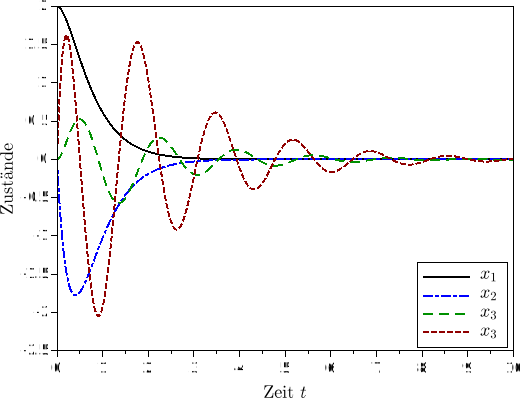
\includegraphics[width=0.85\textwidth]{Wagen-Pendel-Simulation}
\par\end{centering}
\caption{Simulationsergebnis des geregelten Wagen-Pendel-Systems\label{fig:Simulation-Wagen-Pendel-System}}
\end{figure}

\begin{remark}
\label{rem:regler-mit-AD}In der Rückführung~(\ref{eq:rueckfuehrung-stabilisierend-x})
können bei hohem relativen Grad umfangreiche symbolische Ausdrücke
auftreten. Bei der Implementierung des Reglers benötigt man nicht
zwangsläufig eine symbolische Darstellung, sondern nur eine Routine,
die den Ausdruck~(\ref{eq:rueckfuehrung-stabilisierend-x}) in jedem
Abtastschritt numerisch auswertet. Diese Funktionswertberechnung lässt
sich sehr effizient mit Hilfe des algorithmischen Differenzierens
implementieren~\cite{roebenack2000at,roebenack2005fgcs,roebenack2007mcmds}.
\end{remark}

\subsection{Nulldynamik}

Die \index{Nulldynamik}Nulldynamik~(\ref{eq:BINF-Nulldynamik})
wurde im vorangegangenen Abschnitt auf Basis der Byrnes-Isidori-Normalform~(\ref{eq:BINF-Matrixform})
definiert. Da die Berechnung dieser Normalform mitunter schwierig
ist, die Stabilitätsaussage der Nulldynamik (Minimalphasigkeit) aber
für die Stabilisierung des Gesamtsystems relevant ist, wird im Folgenden
ein alternativer Weg zur Berechnung der Nulldynamik angegeben~\cite[{Abschnitt~4.3}]{isidori3}. 

Die Nulldynamik erhält man aus der internen Dynamik in Gl.~(\ref{eq:BINF-Matrixform})
durch Nullsetzen des Zustands des ersten Teilsystems, also mit $\xi=0$.
Entsprechend der Definition der Koordinaten $\xi_{1}=h(x),\xi_{2}=L_{f}h(x),\ldots,\xi_{n}=L_{f}^{r-1}h(x)$
des ersten Teilsystems führt die Bedingung $\xi=0$ in Originalkoordinaten
auf die gleichungsdefinierte Untermannigfaltigkeit 
\begin{equation}
\mathcal{Z}^{*}=\left\{ x\in\mathcal{M}\subseteq\R^{n};\;h(x)=0,\;L_{f}h(x)=0,\;\ldots,\;L_{f}^{r-1}h(x)=0\right\} \label{eq:zwangsbedingung-nulldynamik-x}
\end{equation}
des Vektorraums~$\R^{n}$ der Dimension $n-r$. Mit $y=h(x)=0,\ldots,y^{(r-1)}=L_{f}^{r-1}h(x)=0$
ist zwar der Ausgang in einem Punkt Null, könnte aber durch ungünstige
Wahl des Eingangs aus dem Nullpunkt herausbewegt werden. Um $y(t)=0$
für alle $t\geq0$ sicherzustellen muss zusätzlich für die letzte
Differentialgleichung des ersten Teilsystems gelten: 
\[
\dot{\xi}_{r}=\alpha(\xi,\eta)+\beta(\xi,\eta)u\stackrel{!}{=}0.
\]
Daraus leitet sich unmittelbar die zusätzliche Bedingung 
\begin{equation}
u=-\frac{\alpha(\xi,\eta)}{\beta(\xi,\eta)}=-\frac{L_{f}^{r}h(x)}{L_{g}L_{f}^{r-1}h(x)}\label{eq:zwangsbedingung-nulldynamik-u}
\end{equation}
ab. Für das erste Teilsystem gilt somit 
\begin{equation}
\xi(0)=0\;\wedge\;\forall t\geq0:\;\dot{\xi}(t)=0\quad\Longrightarrow\quad\forall t\geq0:\;\xi(t)=0,\label{eq:nulldyn-TS1}
\end{equation}
woraus auch $y(t)=\xi_{1}(t)=0$ für alle $t\geq0$ folgt.

Mit der Zwangsbedingung~(\ref{eq:zwangsbedingung-nulldynamik-u})
kann man im zweiten Teilsystem der Eingangs-Ausgangs-Normalform~(\ref{eq:EANF-Matrixform})
den Eingangs~$u$ eliminieren
\[
\begin{array}{cll}
\dot{\eta} & = & q(\xi,\eta)+d(\xi,\eta)u\\
 & = & q(\xi,\eta)-d(\xi,\eta)\frac{\alpha(\xi,\eta)}{\beta(\xi,\eta)}\\
 & =: & \tilde{q}(\xi,\eta)
\end{array}
\]
und erhält damit die durch~$\tilde{q}$ beschriebene interne Dynamik
der Byrnes-Isidori-Normalform~(\ref{eq:BINF-Matrixform}). Zusammen
mit Gl.~(\ref{eq:nulldyn-TS1}) ergibt sich daraus die Nulldynamik\index{Nulldynamik}
\begin{equation}
\dot{\eta}=\tilde{q}(0,\eta).\label{eq:nulldyn-TS2}
\end{equation}

In den Originalkoordinaten geht das zu regelnde System~(\ref{eq:Ausgangssystem-fuer-BINF})
mit der Bedingung~(\ref{eq:zwangsbedingung-nulldynamik-u}) in das
autonome System 
\begin{equation}
\dot{x}=f(x)+g(x)u=f(x)-\frac{L_{f}^{r}h(x)}{L_{g}L_{f}^{r-1}h(x)}g(x)=:f^{*}(x)\label{eq:nulldynamik-f-stern}
\end{equation}
mit dem Vektorfeld~$f^{*}$ über. In den transformierten Koordinaten
entspricht dieses Vektorfeld der Nulldynamik~(\ref{eq:nulldyn-TS2}).
Zusammen mit~(\ref{eq:nulldyn-TS1}) ist die Nulldynamik (bezogen
auf den gesamten Zustandsraum $\R^{n}\cong\R^{r}\times\R^{n-r}$ bzw.
eine offenen Teilmenge davon) des Systems~(\ref{eq:EANF-Matrixform})
invariant bezüglich des durch $\xi=0$ definierten Teilraums $(\xi,\eta)\in0\times\R^{n-r}$.
In den Originalkoordinaten entspricht dieser Teilraum der in Gl.~(\ref{eq:zwangsbedingung-nulldynamik-x})
definierten Untermannigfaltigkeit~$\mathcal{Z}^{*}$ (siehe Abb.~\ref{fig:Nulldynamik}).

\begin{figure}
\begin{centering}
\resizebox{0.85\textwidth}{!}{\input{Nulldynamik.pdftex_t}}
\par\end{centering}
\caption{Darstellung der Nulldynamik\index{Nulldynamik} als Vektorfeld~$f^{*}$
auf der Untermannigfaltigkeit~$\mathcal{Z}^{*}$\label{fig:Nulldynamik}}

\end{figure}

Der Zusammenhang zwischen der Untermannigfaltigkeit~$\mathcal{Z}^{*}$
und dem Vektorfeld~$f^{*}$ wird zunächst an einem rein mathematischen
Beispiel illustriert. Der Stabilitätsaspekt spielt dabei keine Rolle,
da das System nicht in einer Ruhelage betrachtet wird.
\begin{example}
\label{exa:nulldynamik-fstar}Das auf $\mathcal{M}=\R^{2}$ definierte
System
\[
\begin{array}{lcl}
\dot{x}_{1} & = & -x_{2}+x_{1}(1-x1^{2}-x_{2}^{2})+x_{1}u\\
\dot{x}_{2} & = & \phantom{-}x_{1}+x_{2}(1-x1^{2}-x_{2}^{2})+x_{2}u\\
y & = & x_{1}^{2}+x_{2}^{2}-1
\end{array}
\]
hat die Form~(\ref{eq:Ausgangssystem-fuer-BINF}) und wegen $L_{g}h(x)=2(x_{1}^{2}+x_{2}^{2})$
den relativen Grad $r=1$. Die Menge $\mathcal{Z}^{*}=\{x\in\R^{2};\;h(x)=x_{1}^{2}+x_{2}^{2}-1=0\}$
nach Gl.~(\ref{eq:zwangsbedingung-nulldynamik-x}) ist der Einheitskreis.
Die Nulldynamik wird durch die Abbildung $f^{*}(x)=-x_{2}\tfrac{\partial}{\partial x_{1}}+x_{1}\tfrac{\partial}{\partial x_{2}}$
nach Gl.~(\ref{eq:nulldynamik-f-stern}) beschrieben. Abb.~\ref{fig:nulldynamik-fstar}
verdeutlicht, dass $f^{*}:\mathcal{Z}^{*}\to\R^{2}$ tangential zu~$\mathcal{Z}^{*}$
liegt, also wirklich ein Vektorfeld ist. Die Nulldynamik entspricht
offensichtlich einer kontinuierlichen Zunahme des Winkels in der $(x_{1},x_{2})$-Ebene.
Das lässt sich durch Berechnung der Byrnes-Isidori-Normalform
\[
\begin{array}{lcl}
\dot{\xi} & = & -2\xi(\xi+1)+2(\xi+1)u\\
\dot{\eta} & = & 1\\
y & = & \xi
\end{array}
\]
verifizieren, wobei für die Hintransformation $\xi=h(x)=x_{1}^{2}+x_{2}^{2}-1$,
$\eta=\arctan(x_{2},x_{1})$ und für die Rücktransformation $x_{1}=\sqrt{\xi+1}\,\cos\eta$,
$x_{2}=\sqrt{\xi+1}\,\sin\eta$ verwendet werden.\footnote{Der Arkustangens $\arctan(x_{2},x_{1})$ mit zwei Argumenten ermöglicht
die Ermittlung des Winkels für alle vier Quadranten (mit Ausnahme
des Nullpunkts). Im ersten Quadranten stimmt diese Funktion mit $\arctan(x_{2}/x_{1})$
überein.}
\end{example}
\begin{figure}
\begin{centering}
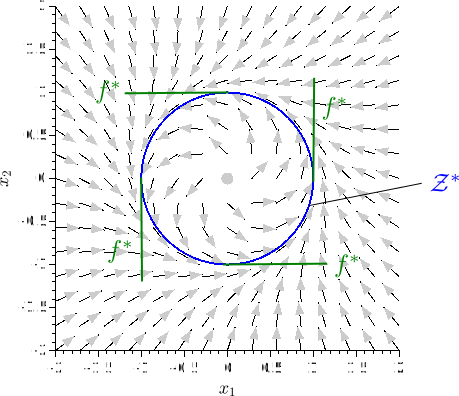
\includegraphics[width=0.65\textwidth]{nulldynamik_fstar}
\par\end{centering}
\caption{Phasen\-ebene zu Beispiel~\ref{exa:nulldynamik-fstar}: Vektorfeld
$f:\mathcal{M}\to\R^{2}$, Unter\-mannig\-faltig\-keit~$\mathcal{Z}^{*}$,
Vektor\-feld $f^{*}:\mathcal{Z}^{*}\to\R^{2}$ \label{fig:nulldynamik-fstar}}
\end{figure}

Bei den nächsten Beispielen wurde die Nulldynamik bereits über die
Byrnes-Isidori-Normalform berechnet. Die nachfolgenden Überlegungen
sind als Kontrollrechnung zu verstehen.

\begin{example}
\label{exa:mobiler-roboter-nulldynamik2}Für das Modell~(\ref{eq:roboter-rg-dgl})
des mobilen Roboters aus Beispiel~\ref{exa:Roboter-rel-grad} mit
dem Ausgang aus Beispiel~\ref{exa:Roboter-geregelt1} wurde der relative
Grad $r=2$ ermittelt. Zur Berechnung der Nulldynamik setzt man die
ersten $r=2$ Lie-Ableitungen (siehe Gl.~(\ref{eq:Roboter-BI-NF-hin1})
aus Beispiel~\ref{exa:Roboter-BI-NF}) zu Null, d.\,h. $x_{1}=0$
und $\sin x_{3}=0$. Wegen $L_{f}^{2}h(x)\equiv0$ vereinfacht sich
die Bedingung~(\ref{eq:zwangsbedingung-nulldynamik-u}) zu $u=0$.
Aus Gl.~(\ref{eq:roboter-rg-dgl}) erhält man damit folgendes autonomes
System: 
\[
\begin{array}{lclcl}
\dot{x}_{1} & = & 0\\
\dot{x}_{2} & = & \cos(\arcsin(0)) & = & \pm1\\
\dot{x}_{3} & = & 0
\end{array}
\]
Die resultierende Nullynamik $\dot{x}_{2}=\pm1$ beschreibt eine Bewegung
des Roboters parallel zur $x_{2}$-Achse. Die zwei Lösungen ergeben
sich entsprechend der Orientierung des Roboters, d.\,h. aus der Koordinate~$x_{3}$.
Für $x_{3}\in(-\pi/2,+\pi/2)$ erhält man in Übereinstimmung mit den
Beispielen~\ref{exa:Roboter-BI-NF} bzw.~\ref{exa:mobiler-roboter-nulldynamik1}
die Nulldynamik $\dot{x}_{2}=1$.
\end{example}

\begin{example}
\label{exa:wagen-pendel-system-nulldynamik2}Man betrachte das Wagen-Pendel-System
aus Beispiel~\ref{exa:Wagen-Pendel-partielle-Linearisierung}. Die
Bedingung~(\ref{eq:zwangsbedingung-nulldynamik-u}) erfüllt man im
partiell linearisierten System durch $v=0$. Damit geht Gl.~(\ref{eq:wagen-pendel-kollokiert-linearisiert})
in das System 
\begin{equation}
\begin{array}{lcl}
\dot{x}_{1} & = & 0\\
\dot{x}_{2} & = & 0\\
\dot{x}_{3} & = & x_{4}\\
\dot{x}_{4} & = & -\frac{d_{2}}{\ell^{2}m_{2}}x_{4}-\frac{g}{\ell}\sin x_{3}
\end{array}\label{eq:wagen-pendel-nulldynamik2}
\end{equation}
über. Die letzten zwei Differentialgleichungen stimmen mit der in
Beispiel~\ref{exa:wagen-pendel-system-nulldynamik1} berechneten
Nulldynamik überein.
\end{example}

\begin{remark}
\label{rem:Nulldynamik-Nullstellen-Uebertragungsfunktion}Die Nulldynamik
spiegelt sich bei einem linearen System auch in der Übertragungsfunktion
wider. Man betrachte das geregelte System~(\ref{eq:BINF-Stabilisiert})
mit der Systemmatrix $A_{11}:=A-bk^{T}$ des ersten Teilsystems~(\ref{eq:BINF-Stabilisiert1})
und einem linearen zweiten Teilsystem~(\ref{eq:BINF-Stabilisiert2}),
welches durch $q(\xi,\eta)=A_{21}\xi+A_{22}\eta$ mit $A_{21}\in\R^{(n-r)\times r}$
und $A_{22}\in\R^{(n-r)\times(n-r)}$ gegeben sei. Das Gesamtsystem
lautet dann 
\begin{equation}
\begin{array}{ccl}
\left(\begin{array}{c}
\dot{\xi}\\
\dot{\eta}
\end{array}\right) & = & \overbrace{\left(\begin{array}{cc}
A_{11} & 0\\
A_{21} & A_{22}
\end{array}\right)}^{{\displaystyle \bar{A}}}\left(\begin{array}{l}
\xi\\
\eta
\end{array}\right)+\overbrace{\left(\begin{array}{l}
b\\
0
\end{array}\right)}^{{\displaystyle \bar{b}}}u\\
y & = & \underbrace{\left(\begin{array}{cc}
c^{T} & 0\end{array}\right)}_{{\displaystyle \bar{c}^{T}}}\left(\begin{array}{l}
\xi\\
\eta
\end{array}\right).
\end{array}\label{eq:rel-grad-lineares-Gesamtsystem-ND}
\end{equation}
Die Übertragungsfunktion kann einererseits in der Form 
\begin{eqnarray}
G(s) & = & \frac{b_{n-r}s^{n-r}+\cdots+b_{1}s+b_{0}}{\det\left(sI_{n}-\bar{A}\right)}\nonumber \\
 & = & \frac{b_{n-r}s^{n-r}+\cdots+b_{1}s+b_{0}}{\det\left(sI_{r}-A_{11}\right)\cdot\det\left(sI_{n-r}-A_{22}\right)}\label{eq:rel-grad-UF1}
\end{eqnarray}
angesetzt werden. Der Nenner besteht aus dem charakteristischen Polynom
der Systemmatrix~$\bar{A}$. Wegen der Block\-dreiecks\-struktur
von~$\bar{A}$ zerfällt das charakteristische Polynom in das Produkt
der charakteristischen Polynome der Matrizen~$A_{11}$ und~$A_{22}$.
Bei einem relativen Grad~$r$ und einem Nennerpolynom vom Grad~$n$
weist das Zählerpolynom den Grad $n-r$ auf (siehe Anmerkung~\ref{rem:rel-grad-Uebertragungsfunktion}).
Andererseits kann man die Übertragungsfunktion unter Beachtung der
Block\-dreiecks\-struktur von~$\bar{A}$ direkt ausgerechnet werden:
\begin{eqnarray}
G(s) & = & \bar{c}^{T}\left(sI_{n}-\bar{A}\right)^{-1}\bar{b}\nonumber \\
 & = & \left(\begin{array}{cc}
c^{T} & 0\end{array}\right)\left(\begin{array}{cc}
sI_{r}-A_{11} & 0\\
-A_{21} & sI_{n-r}-A_{22}
\end{array}\right)^{-1}\left(\begin{array}{l}
b\\
0
\end{array}\right)\nonumber \\
 & = & \left(\begin{array}{cc}
c^{T} & 0\end{array}\right)\left(\begin{array}{cc}
\left(sI_{r}-A_{11}\right)^{-1} & 0\\
* & \left(sI_{n-r}-A_{22}\right)^{-1}
\end{array}\right)\left(\begin{array}{l}
b\\
0
\end{array}\right)\nonumber \\
 & = & c^{T}\left(sI_{r}-A_{11}\right)^{-1}b\nonumber \\
 & = & \frac{c^{T}\adj\left(sI_{r}-A_{11}\right)\,b}{\det\left(sI_{r}-A_{11}\right)}.\label{eq:rel-grad-UF2}
\end{eqnarray}
Das Zählerpolynom wird mit der Matrix der Adjunkten bzw. Kofaktoren
gebildet~\cite{reinschke88}. Das Nennerpolynom ist das charakteristische
Polynom der Matrix~$A_{11}$ und hat damit den Grad~$r$. Nach Anmerkung~\ref{rem:rel-grad-Uebertragungsfunktion}
muss auch bei Gl.~(\ref{eq:rel-grad-UF2}) zwischen Zähler- und Nennergrad
die Differenz~$r$ auftreten, so dass der Nenner in Gl.~(\ref{eq:rel-grad-UF2})
konstant sein muss. Ohne Einschränkungen sei der Nenner Eins. Die
unterschiedlichen Nennergrade von~(\ref{eq:rel-grad-UF1}) und~(\ref{eq:rel-grad-UF2})
lassen sich dadurch erklären, dass das zweite Teil\-system nicht
beobachtbar ist und daher in der Übertragungsfunktion zwischen Zähler
und Nenner gekürzt werden kann (siehe auch Beispiel~\ref{exa:Lineares-System-r-infty}).
Der Vergleich zwischen~(\ref{eq:rel-grad-UF1}) und~(\ref{eq:rel-grad-UF2})
führt damit unmittelbar auf
\[
b_{n-r}s^{n-r}+\cdots+b_{1}s+b_{0}=\det\left(sI_{n-r}-A_{22}\right),
\]
so dass das Zählerpolynom von~(\ref{eq:rel-grad-UF1}) das charakteristische
Polynom der Matrix~$A_{22}$ ist. Die Eigenwerte der Systemmatrix
$A_{22}$ der Nulldynamik von~(\ref{eq:rel-grad-lineares-Gesamtsystem-ND})
fallen folglich mit den Nullstellen der Übertragungsfunktion~(\ref{eq:rel-grad-UF1})
zusammen.
\end{remark}

Bei komplizierten Systemen kann man versuchen, die Stabilität der
Nulldynamik durch Taylor-Linearisierung in den Originalkoordinaten
zu untersuchen. Die zur Berechnung der Nulldynamik angegebene Bedingung~(\ref{eq:zwangsbedingung-nulldynamik-u})
kann man dabei auch als eine Vorgabe von $r$ Eigenwerten bei Null
verstehen. Nach einer Taylor-Linearisierung des resultierenden Systems~(\ref{eq:nulldynamik-f-stern})
in der betreffenden Ruhelage sind die verbleibenden $n-r$ Eigenwerte
der Jacobi\-matrix der Nulldynamik zuzuordnen. Besitzen alle Eigenwerte
der Nulldynamik einen nichtverschwindenden Realteil, so liegt für
die Nulldynamik eine \emph{hyperbolische Ruhelage}\index{Ruhelage!hyperbolische}
vor. Nach dem Satz von Hartman-Grobman\index{Satz!von Hartman-Grobman}
ist bei einer hyperbolischen Ruhelage das nichtlineare System in einer
Umgebung der betreffenden Ruhelage topologisch konjugiert\index{topologisch konjugiert}
bzw. zustandsäquivalent\index{zustandsäquivalent} zu seiner Taylor-Linearisierung~\cite{guckenheimer83,arrowsmith90}.
Besitzen alle der Nulldynamik zugeordneten $n-r$ Eigenwerte einen
negativen Realteil, so ist die Ruhelage (lokal) asymptotisch stabil.
Gibt es einen Eigenwert mit positivem Realteil, dann ist die Ruhelage
instabil. Weist die Linearisierung der Nulldynamik dagegen einen Eigenwert
mit Realteil Null auf, dann ist die Ruhelage nicht hyperbolisch. (Bezogen
auf die Linearisierung des Gesamtsystems bedeutet das, dass es mehr
als $r$ Eigenwerte bei Null gibt oder ein rein imaginäres Eigenwertpaar
auftritt.) Selbst wenn alle anderen Eigenwerte einen negativen Realteil
besitzen ist in diesem Fall keine Stabilitätsaussage auf Basis der
Linearisierung möglich. Die Stabilität der Ruhelage könnte man dann
mit Hilfe des Satzes über die Zentrumsmannigfaltigkeit\index{Satz!über die Zentrumsmannigfaltigkeit}
untersuchen~\cite{guckenheimer83,arrowsmith90}.
\begin{example}
Die Taylor-Linearisierung von~(\ref{eq:wagen-pendel-nulldynamik2})
im Ursprung $x=0$ führt auf das System
\[
\left(\begin{array}{c}
\dot{x}_{1}\\
\dot{x}_{2}\\
\dot{x}_{3}\\
\dot{x}_{4}
\end{array}\right)=\left(\begin{array}{cccc}
0 & 0 & 0 & 0\\
0 & 0 & 0 & 0\\
0 & 0 & 0 & 1\\
0 & 0 & -\frac{g}{l} & -\frac{d_{2}}{l^{2}m_{2}}
\end{array}\right)\left(\begin{array}{l}
x_{1}\\
x_{2}\\
x_{3}\\
x_{4}
\end{array}\right)
\]
mit dem charakteristischen Polynom 
\[
s^{2}\cdot\left(s^{2}+\frac{d_{2}}{l^{2}m_{2}}s+\frac{g}{l}\right).
\]
Die doppelte Nullstelle bei $s=0$ resultiert unmittelbar aus der
Bedingung~(\ref{eq:nulldyn-TS1}). Das verbleibende Polynom zweiter
Ordnung ist nach der Stodola-Bedingung (siehe~\cite{reinschke2014buch})
für die relevanten Parameterwerte $g,l,d_{2},m_{2}>0$ ein Hurwitz-Polynom.
Alle Eigenwerte der Nulldynamik besitzen somit einen negativen Realteil.
Die Ruhelage $\eta=0$ ist daher (lokal) asymptotisch stabil. 
\end{example}

\subsection{Äquivalenz von Systemen und globale Stabilisierung\label{subsec:Equivalenz-globale-Stab}}

Setzt man die linearisierende Rückführung~(\ref{eq:rueckfuehrung-linearisierend})
in die Systemgleichungen~(\ref{fig:Ausgangssystem-fuer-BINF}) ein,
so erhält man das System 
\begin{equation}
\begin{array}{lcl}
\dot{x} & = & f(x)+g(x)u\\
 & = & f(x)+g(x)\frac{1}{L_{g}L_{f}^{r-1}h(x)}\left(v-L_{f}^{r}h(x)\right)\\
 & = & \underbrace{f(x)-\frac{L_{f}^{r}h(x)}{L_{g}L_{f}^{r-1}h(x)}g(x)}_{{\displaystyle f^{*}(x)}}+\underbrace{\frac{1}{L_{g}L_{f}^{r-1}h(x)}g(x)}_{{\displaystyle g^{*}(x)}}\,v
\end{array}\label{eq:linearisiertes-System-in-x}
\end{equation}
mit den Vektorfeldern~$f^{*}$ und~$g^{*}$. Das System~(\ref{eq:linearisiertes-System-in-x})
wird in einer Umgebung des Punktes~$p$ durch den (lokalen) Diffeomorphismus~$\Phi$
in das System~(\ref{eq:BINF-Linearisiert}) überführt. Diese Systeme
sind dann \emph{zustands\-äquivalent}\index{zustandsäquivalent}
(engl. \emph{state equivalent}), siehe~\cite{dayawansa1985}. (Damit
wird der in Kapitel~\ref{chap:Diff-Geo} eingeführte Begriff der
Zustands\-äquivalenz auf Systeme mit Eingang erweitert.) Ist die
Zustands\-transformation~$\Phi$ ein globaler Diffeomorphismus,
so nennt man die Systeme \emph{global zustands\-äquivalent}. Im Allgemeinen
sind die Existenzbedingungen für eine globale Transformation sehr
restriktiv. Für den Fall, dass man die Transformation explizit ausrechnen
kann und $\mathcal{M}=\R^{n}$ gilt, sind in~\cite{wu72} überprüfbare
Bedingungen angegeben.

Bei einem im Punkt $p\in\mathcal{M}$ wohldefinierten relativen Grad~$r$
ist das System~(\ref{fig:Ausgangssystem-fuer-BINF}) in einer Umgebung
von~$p$ zustandsäquivalent zu einem System der Bynres-Isidori-Normalform~(\ref{eq:BINF-Matrixform}).
Eine notwendige Bedingung für eine globale Zustandsäquivalenz ist
ein konstanter relativer Grad:
\begin{definition}
\label{def:gleichmaessiger-relativer-grad}System~(\ref{fig:Ausgangssystem-fuer-BINF})
hat einen \emph{gleichmäßigen relativen Grad}\index{relativer Grad!gleichmäßiger}
(engl. \emph{uniform relative degree}), falls es den relativen Grad~$r$
nach Definition~\ref{def:relativer-Grad-SISO} für alle $p\in\mathcal{M}$
besitzt.
\end{definition}
Basierend auf \cite{byrnes91nf} und~\cite[Kapitel~9]{isidori3}
lässt sich folgende Existenzaussage treffen:
\begin{theorem}
\label{them:globale-BINF}Wir betrachten System~(\ref{fig:Ausgangssystem-fuer-BINF})
auf einer offenen und zusammenhängenden Menge $\mathcal{M}\subseteq\R^{n}$.
Das System habe einen gleichmäßigen relativen Grad~$r$. Ferner gelte~(\ref{eq:Ruhelage-x})
und~(\ref{eq:Ruhelage-y}). Sind die Vektorfelder 
\begin{equation}
g^{*},\ad_{-f^{*}}g^{*},\ldots,\ad_{-f^{*}}^{r-1}g^{*}:\mathcal{M}\to\R^{n}\label{eq:VF-ad-g-tilde}
\end{equation}
vollständig\index{Vektorfeld!vollständiges}\footnote{Ein Vektorfeld heißt \textit{vollständig}, wenn es einen globalen
Fluss besitzt (vgl. Abschnitt~\ref{sec:Vektorfelder-und-Fluesse}).}, so ist das System~(\ref{eq:linearisiertes-System-in-x}) global
zustandsäquivalent zu einem System der Form~(\ref{eq:BINF-Linearisiert}).
\end{theorem}
Mit Gln.~(\ref{eq:Ruhelage-x}) und~(\ref{eq:Ruhelage-y}) ist die
Menge~$\mathcal{Z}^{*}$ nicht leer. Dann ist sie auch zusammenhängend.
Die Koordinatentransformation wird über die Flussverkettung der Vektorfelder~(\ref{eq:VF-ad-g-tilde})
konstruiert. Allerdings ist es in der Regel nicht leicht zu überprüfen,
ob ein gegebenes Vektorfeld vollständig ist. Eine Möglichkeit dazu
bietet der Satz von Wintner und Conti~\cite{reitmann96}.

\medskip{}

Der Übergang vom gegebenen System~(\ref{fig:Ausgangssystem-fuer-BINF})
zu der Form~(\ref{eq:linearisiertes-System-in-x}) erfolgt durch
die Rück\-führung~(\ref{eq:rueckfuehrung-linearisierend}). Zwei
Systeme heißen \emph{äquivalent unter statischer Zustandsrückführung},
(kurz \emph{rück\-führ\-äquivalent}\index{rückführäquivalent}
(engl. \emph{feed\-back equivalent}), wenn es eine statische Zustandsrückführung
gibt, so dass die Systeme zustandsäquivalent sind. Die Systeme heißen
\emph{global rück\-führ\-äquivalent}, falls die betrachteten Systeme
unter einer auf ganz $\mathcal{M}$ definierten Zustandsrückführung
global zustands\-äquivalent sind. Durch die Kombination aus Zustandstransformation
und Zustandsrückführung kann man die Systeme ineinander überführen.
In diesem Sinne sind die Systeme~(\ref{fig:Ausgangssystem-fuer-BINF})
und~(\ref{eq:linearisiertes-System-in-x}) rückführäquivalent, wobei
die Rückführung durch Gl.~(\ref{eq:rueckfuehrung-linearisierend})
gegeben ist. Das folgende Diagramm illustriert die Äquivalenzen einiger
der bisher betrachteten Systeme:

\[
\begin{tikzcd}
\text{(System~\ref{eq:Ausgangssystem-fuer-BINF})} 
\arrow[leftrightarrow]{rr}[above]{\stackrel{\textstyle\text{zustands-}}{\textstyle\text{äquivalent}}} 
\arrow[leftrightarrow]{d}[left]{\stackrel{\textstyle\text{rückführ-}}{\textstyle\text{äquivalent}}\quad} \arrow[rrd, leftrightarrow] 
& {} & \text{System~(\ref{eq:BINF-Matrixform})} 
\arrow[leftrightarrow]{d}[right]{\quad\stackrel{\textstyle\text{rückführ-}}{\textstyle\text{äquivalent}}}
\arrow[lld, leftrightarrow, crossing over]\\ 
\text{System~(\ref{eq:linearisiertes-System-in-x})} 
\arrow[leftrightarrow]{rr}[below]{\stackrel{\textstyle\text{zustands-}}{\textstyle\text{äquivalent}}} 
& {} & \text{System~(\ref{eq:BINF-Linearisiert})}
\end{tikzcd}
\]

Die lokale Stabilisierung des Systems~(\ref{fig:Ausgangssystem-fuer-BINF})
mittels Eingangs-Ausgangs-Linearisierung setzt nach Satz~\ref{thm:Stabilisierung-EA-lokal}
die lokale asymptotische Stabilität der Nulldynamik~(\ref{eq:BINF-Nulldynamik})
voraus. Für eine globale Stabilisierung nach dem gleichen Schema (also
mit einer linearen Rückführung im eingangs-ausgangs-linearisierten
ersten Teilsystem) ist selbst die globale asymptotische Stabilität
der Nulldynamik~(\ref{eq:BINF-Nulldynamik}) nicht hinreichend~\cite{sussmann1990}.
Das nachfolgende Beispiel wurde~\cite[Example~{4.2}]{sepulchre97}
entnommen:

\begin{example}
\label{exa:keine-globale-stabiliserung-mit-linearer-rueckf}Das System
\[
\begin{array}{lcl}
\dot{\xi} & = & u\\
\dot{\eta} & = & -\eta+\eta^{2}\xi
\end{array}
\]
liegt bereits in der partiell linearisierten Form~(\ref{eq:BINF-Linearisiert})
vor. Die Rückführung $u=-k\xi$ mit $k>0$ sichert die globale asymptotische
Stabilität der Ruhelage $\xi=0$ des ersten Teilsystems. Die Nulldynamik
$\dot{\eta}=-\eta$ ist ebenfalls global asymptotisch stabil. Damit
ist die Ruhelage $(\xi,\eta)=(0,0)$ lokal asmptotisch stabil, aber
nicht global: Der Anfangswert $\xi(0)=1$ liefert für das rückgeführte
erste Teilsystem die Lösung $\xi(t)=\e^{-t}$. Setzt man diese Lösung
in das zweite Teilsystem ein, so ergibt sich für den Anfangswert $\eta(0)=p$
die Lösung
\[
\eta(t)=\frac{(k+1)p\e^{-t}}{p\e^{-(k+1)t}-p+k+1}.
\]
Geht man von $p>0$ aus, so hat die Lösung für $p>k+1$ eine Polstelle
und damit eine endliche Fluchtzeit (vgl. auch Beispiel~\ref{exa:EndlicheFluchtzeit}).

Ein aussagekräftiges Konzept für eine globale Stabilitätsaussage ist
die \emph{Eingangs-Zustands-Stabilität} (engl. \emph{input-state stability},
kurz \emph{ISS}), siehe~\cite{sontag1995ejc,sontag2000} und Anhang~\ref{sec:Stabilitaet-erregter-Systeme}.
Wir nennen ein System \emph{stark minimalphasig}\index{minimalphasig!stark}
(engl. \emph{strongly minimum phase}), wenn die interne Dynamik nach
Gl.~(\ref{eq:BINF-Stabilisiert2}) eingangs-zustands-stabil\index{eingangs-zustands-stabil}
bezüglich~$\xi$ (als Eingang) ist~\cite{liberzon2000,isidori2013ejc}.
\end{example}
\begin{theorem}
\label{thm:Stabilisierung-EA-global}Das System~(\ref{eq:Ausgangssystem-fuer-BINF})
habe den Arbeitspunkt $p\in\mathcal{M}$ (für $u=0$) und den gleichmäßigen
relativen Grad $r<n$. Zusätzlich sei das System global rück\-führ\-äquivalent
zu der Form~(\ref{eq:BINF-Stabilisiert}) mit der Ruhelage $(\xi,\eta)=(0,0)$.
Die Reglerverstärkung $k\in\R^{r}$ sei so gewählt, dass das charakteristische
Polynom~(\ref{eq:TS1-charakteristisches-Polynom}) ein Hurwitz-Polynom
ist. Ist das System stark minimalphasig, dann ist die Ruhelage~$p$
des resultierenden Systems global asymptotisch stabil.
\end{theorem}
\begin{svmultproof2}
Durch die Wahl der Reglerverstärkung~$k$ besitzt die Matrix $A-bk^{T}$
nur Eigenwerte mit negativem Realteil. Die Ljapunov-Funktion~$V_{1}$
für das erste Teil\-system~(\ref{eq:BINF-Stabilisiert1}) lässt
sich daher wie im Beweis von Satz~(\ref{thm:Stabilisierung-EA-lokal})
über die Ljapunov-Gleichung~(\ref{eq:TS1-Lyap-Gleichung}) konstruieren.
Außerdem wurde angenommen, dass das zweite Teilsystem~(\ref{eq:BINF-Stabilisiert2})
eingangs-zustands-stabil bezüglich~$\xi$ ist. Damit liegt eine Kaskadenstruktur
entsprechend Abb.~\ref{fig:Kaskadenstruktur-EA-Linearisierung} vor.
Entsprechend Anhang~\ref{sec:Stabilitaet-erregter-Systeme} ist damit
die Ruhelage $(\xi,\eta)=(0,0)$ global asymptotisch stabil.
\end{svmultproof2}

Erweitert man die Rückführung~(\ref{eq:rueckfuehrung-stabilisierend})
wie in Gl.~(\ref{eq:regler4-linearisierung-stabilisierung-sollwert-y})
mit um einen Eintrag hinsichtlich der Führungsgröße~$w$, so erhält
man für das Eingangs-Ausgangs-Verhalten des ersten Teilsystems
\begin{equation}
\begin{array}{lcl}
\dot{\xi} & = & \left(A-bk^{T}\right)\xi+a_{0}bw\\
y & = & c^{T}\xi
\end{array}\label{eq:TS1-stabilisiert-mit-Fuerungsgroesse}
\end{equation}
die Übertragungsfunktion~(\ref{eq:UF-WY}). Die Rückführung kann
in Originalkoordinaten durch Gl.~(\ref{eq:regler4-linearisierung-stabilisierung-sollwert-x})
ausgedrückt werden. Für den Fall eines sich zeitlich veränderlichen
Verlauf der Führungsgröße~$w$ liegt keine Ruhelage vor. Daher ist
auch die asymptotische Stabilität nicht sehr hilfreich. Im Falle eines
eingangs-zustands-stabilen Systems hat man die Gewissheit, dass bei
einem beschränkten Eingangs- bzw. Führungssignal~$w$ der Zustand
ebenfalls beschränkt bleibt.
\begin{theorem}
\label{thm:Stabilisierung-EA-global-fuehrungssignal}Das System~(\ref{eq:Ausgangssystem-fuer-BINF})
habe den Arbeitspunkt $p\in\mathcal{M}$ (für $u=0$) und den gleichmäßigen
relativen Grad $r<n$. Zusätzlich sei das System global rück\-führ\-äquivalent
zu der Form~(\ref{eq:TS1-stabilisiert-mit-Fuerungsgroesse}), (\ref{eq:BINF-Stabilisiert2})
mit der Ruhelage $(\xi,\eta)=(0,0)$. Die Reglerverstärkung $k\in\R^{r}$
sei so gewählt, dass das charakteristische Polynom~(\ref{eq:TS1-charakteristisches-Polynom})
ein Hurwitz-Polynom ist. Ist das System stark minimalphasig, dann
ist das resultierende Gesamtsystem eingangs-zustands-stabil.
\end{theorem}
\begin{svmultproof2}
Laut Annahme hat die Matrix $A-bk^{T}$ nur Eigenwerte mit negativem
Realteil. Das lineare Teilsystem~(\ref{eq:TS1-stabilisiert-mit-Fuerungsgroesse})
ist daher eingangs-zustands-stabil. Das zweite Teilsystem~(\ref{eq:BINF-Stabilisiert2})
ist ebenfalls eingangs-zustands-stabil. Damit ist auch das Gesamtsystem
eingangs-zustands-stabil (siehe Anhang~\ref{sec:Stabilitaet-erregter-Systeme}).
\end{svmultproof2}

In den Sätzen~\ref{thm:Stabilisierung-EA-global} und~\ref{thm:Stabilisierung-EA-global-fuehrungssignal}
wurde die Annahme der Minimalphasigkeit, d.\,h. der asymptotischen
Stabilität der Nulldynamik~(\ref{eq:BINF-Nulldynamik}), durch die
Eigenschaft der Eingangs-Zustands-Stabilität ersetzt. Andere Möglichkeiten
zur Charakterisierung der Stabilität der internen Dynamik sind beispielsweise
in~\cite{krichman1999,liberzon2000} angegeben.

\section{Exakte Eingangs-Zustands-Linearisierung\label{sec:Exakte-Eingangs-Zustands-Linearisierung}}

\subsection{Problemformulierung\label{subsec:EZ-Linearisierung-Problemformulierung}}

Bei der Eingangs-Ausgangs-Linearisierung eines Systems~(\ref{eq:Ausgangssystem-fuer-BINF})
mit relativem Grad~$r$ erhält man ein lineares erstes Teilsystem
der Dimension~$r$. Für $r<n$ verbleibt im Gesamtsystem ein nicht
zu beeinflussendes und in der Regel nichtlineares zweites Teilsystem
des Dimension $n-r$. Es stellt sich folgende Frage: Wann kann ein
System 
\begin{equation}
\dot{x}=f(x)+g(x)u\label{eq:system-fuer-eingangs-zustands-lin}
\end{equation}
mit glatten Vektorfeldern $f,g:\mathcal{M}\to\R^{n}$ in einer Umgebung
eines Punktes $p\in\mathcal{M}$ \textit{vollständig} in ein lineares
steuerbares System überführt werden, so dass kein zweites Teil\-system
übrigbleibt? Dieses Problem der \emph{(exakten) Eingangs-Zustands-Linearisierung}\index{Linearisierung!Eingangs-Zustands-}
ist lösbar, wenn es eine Ausgangsabbildung $h:\mathcal{M}\to\R$ gibt
(d.\,h. ein Skalarfeld), so dass das System~(\ref{eq:system-fuer-eingangs-zustands-lin})
den relativen Grad~$n$ besitzt. Ein solches System nennt man \emph{eingangs-zustands-linearisierbar}. 

Bei vielen Systemen ist aus Sicht des Anwenders bereits ein Ausgang
als Regel- oder Messgröße vorgegeben, für den das System im Sinne
der Eingangs-Ausgangs-Linearisierung einen (festen) relativen Grad~$r$
besitzt. Bei der Eingangs-Zustands-Linearisierung sucht man einen
(zunächst als reine Hilfsgröße eingeführten) Ausgang mit relativem
Grad~$n$, auf dessen Basis eine Zustandsrückführung entworfen wird.

Bei einem eingangs-zustands-linearisierbaren System gehen sowohl die
Eingangs-Ausgangs-Normalform~(\ref{eq:EA-Form-komponentenweise})
als auch die Byrnes-Isidori-Normaform~(\ref{eq:BINF-Komponentenweise})
in die \emph{Regelungsnormalform}\index{Regelungsnormalform}\index{Normalform!Regelungs-}
(engl. \emph{controller canonical form}) 
\begin{equation}
\begin{array}{lcl}
\dot{z}_{1} & = & z_{2}\\
 & \vdots\\
\dot{z}_{n-1} & = & z_{n}\\
\dot{z}_{n} & = & \alpha(z)+\beta(z)u\\
y & = & z_{1}
\end{array}\label{eq:Regelungsnormalform}
\end{equation}
 über (siehe Abb.~\ref{fig:regelungsnormalform} sowie~\cite{zeitz85,zeitz89}).
Entsprechend Gl.~(\ref{eq:alpha-beta-EA-NF}) ergeben sich die Skalarfelder~$\alpha$
und $\beta$ aus 
\begin{equation}
\begin{array}{lcl}
\alpha(z) & = & \left.L_{f}^{n}h(x)\right|_{x=\Phi^{-1}(z)}\\
\beta(z) & = & \left.L_{g}L_{f}^{n-1}h(x)\right|_{x=\Phi^{-1}(z)}
\end{array}\label{eq:alpha-beta-EZ-Regelungs-NF}
\end{equation}
mit $\beta(\Phi(p))\neq0$. Mit der Zustandsrückführung
\begin{equation}
u=\frac{1}{\beta(z)}\left(v-\alpha(z)\right)\label{eq:rueckfuehrung-EZ}
\end{equation}
erhält man aus dem (bedingt durch die Skalarfelder~$\alpha$ und
$\beta$ typischerweise nichtlinearen) System~(\ref{eq:Regelungsnormalform})
ein lineares steuerbares System in Brunovský-Normalform\index{Brunovský-Normalform}\index{Normalform!Brunovský-}~\cite{brunovsky70}
\begin{equation}
\left.\begin{array}{lcl}
\dot{z}_{1} & = & z_{2}\\
 & \vdots\\
\dot{z}_{n-1} & = & z_{n}\\
\dot{z}_{n} & = & v\\
y & = & z_{1}
\end{array}\right\} \quad\begin{array}{ccl}
\dot{x} & = & Ax+bv\\
y & = & c^{T}v
\end{array}\label{eq:Brunovsky-Normalform}
\end{equation}
mit der Matrix $A\in\R^{n\times n}$ und dem Vektor \textbf{$b\in\R^{n}$}
entspr. Gl.~(\ref{eq:Abc-Brunovsky}). Ein System~(\ref{eq:system-fuer-eingangs-zustands-lin})
ist genau dann eingangs-zustands-linearisierbar, wenn es zustands\-äquivalent
zu~(\ref{eq:Regelungsnormalform}) bzw. rück\-führ\-äquivalent
zu~(\ref{eq:Brunovsky-Normalform}) ist.

\begin{figure}
\begin{centering}
\resizebox{0.9\textwidth}{!}{\input{regelungsnormalform.pdftex_t}}
\par\end{centering}
\caption{Regelungsnormalform~(\ref{eq:Regelungsnormalform}) eines eingangsaffinen
Systems~(\ref{eq:Ausgangssystem-fuer-BINF})\label{fig:regelungsnormalform}}
\end{figure}


\subsection{Problemlösung über Distributionen\label{subsec:EZ-Linearisierung-Distributionen}}

System~(\ref{eq:system-fuer-eingangs-zustands-lin}) ist genau dann
in einem Punkt $p\in\mathcal{M}$ eingangs-zustands-linearisierbar,
wenn es eine Ausgangsabbbildung $h:\mathcal{M}\to\R$ (also ein Skalarfeld)
gibt, so dass das System in dem betreffenden Punkt den relativen Grad~$n$
besitzt. Nach der Definition des relativen Grades muss in diesem Fall
\begin{equation}
\begin{array}{rclll}
L_{g}L_{f}^{i}h(x) & = & 0 & \mbox{für} & 0\leq i\leq n-2,\\
L_{g}L_{f}^{n-1}h(p) & \neq & 0
\end{array}\label{eq:ex-ein-zu0}
\end{equation}
für alle~$x$ aus einer Umgebung von~$p$ gelten. Entsprechend Lemma~\ref{lem:Skalarprod-dLf-ad}
gilt daher auch 
\[
L_{\ad_{-f}^{i}g}L_{f}^{j}h=\left\langle \d L_{f}^{j}h,\ad_{-f}^{i}g\right\rangle =\left\{ \begin{array}{ccccc}
0 & \mbox{für} & i+j & < & n-1,\\
L_{g}L_{f}^{n-1}h & \mbox{für} & i+j & = & n-1.
\end{array}\right.
\]
Für $j=0$ erhält man 
\begin{eqnarray}
L_{\ad_{-f}^{i}g}h(x) & = & 0\quad\mbox{for}\quad0\leq i\leq n-2\label{eq:ex-ein-zu1}\\
L_{\ad_{-f}^{n-1}g}h(p) & \neq & 0.\label{eq:ex-ein-zu2}
\end{eqnarray}
Wegen $L_{\ad_{-f}^{i}g}h=\langle\d h,\ad_{-f}^{i}g\rangle$ kann
man die $n-1$ Gleichungen~(\ref{eq:ex-ein-zu1}) auch in der Form
\begin{equation}
\d h(x)\cdot\left(g(x),\ad_{-f}g(x),\ldots,\ad_{-f}^{n-2}g(x)\right)=\left(0,0,\ldots,0\right)\label{eq:ex-ein-zu-PDE}
\end{equation}
angeben. Damit erhält man eine (vektorwertige) partielle Differentialgleichung
erster Ordnung für die Unbekannte~$h$. Zur Untersuchung der Lösbarkeit
wird die Folge 
\begin{equation}
\Delta_{i}(x)=\spann\left\{ g(x),\ad_{-f}g(x),\ldots,\ad_{-f}^{i-1}g(x)\right\} \label{eq:Distributionen-Delta-i}
\end{equation}
von Distributionen\index{Distribution} definiert. Der nachfolgende
Satz gibt die genauen Existenzbedingungen für eine Ausgangsabbildung
mit vollem relativen Grad an~\cite{su1982}, \cite[Theorem~{4.2.3}]{isidori3}:
\begin{theorem}
\label{thm:Exakte-Eingangs-Zustands_Linearisierung}Das System~(\ref{eq:system-fuer-eingangs-zustands-lin})
besitzt im Punkt $p\in\mathcal{M}$ genau dann eine Ausgangsabbildung~$h$
mit relativem Grad~$n$, wenn gilt:
\begin{enumerate}
\item \label{enu:exakt-dim}$\dim\,\Delta_{n}(p)=n$ und
\item \label{enu:exakt-involutiv}$\Delta_{n-1}$ ist involutiv in einer
Umgebung von~$p$.\index{involutive Distribution}\index{Distribution!involutive}
\end{enumerate}
\end{theorem}
\begin{svmultproof2}
\hinreichend\ Das System~(\ref{eq:system-fuer-eingangs-zustands-lin})
habe im Punkt $p\in\mathcal{M}$ den relativen Grad~$n$ für eine
Ausgangsabbildung~$h$. Wegen Lemma~\ref{lem:Skalarprod-dLf-ad}
gilt
\begin{equation}
\begin{array}{l}
\left(\begin{array}{c}
\d h(p)\\
\d L_{f}h(p)\\
\vdots\\
\d L_{f}^{n-1}h(p)
\end{array}\right)\left(g(p),\ad_{-f}g(p),\ldots,\ad_{-f}^{n-1}g(p)\right)=\\
=\left(\begin{array}{cccc}
0 & \cdots & 0 & L_{g}L_{f}^{n-1}h(p)\\
\vdots & \qdots &  & *\\
0 &  & \qdots & \vdots\\
L_{g}L_{f}^{n-1}h(p) & * & \cdots & *
\end{array}\right).
\end{array}\label{eq:beweis-ez-linearisierbarkeit-unabh-VF}
\end{equation}
Daraus folgt $\dim\,\Delta_{n}(p)=n$. Außerdem folgt aus der linearen
Unabhängigkeit der Vektoren $g(p),\ldots,\ad_{-f}^{n-1}g(p)$ auch
$\dim\,\Delta_{n-1}=n-1$. Damit ist die Distribution $\Delta_{n-1}$
im Punkt~$p$ regulär. Aufgrund des relativen Grades~$n$ gilt~(\ref{eq:ex-ein-zu-PDE})
(siehe Vorbetrachtungen zum Satz), d.\,h. der Gradient $\d h$ spannt
den Annihilator von $\Delta_{n-1}$ auf. Nach dem Satz von Frobenius
(Satz~\ref{thm:Frobenius-lokal}) ist $\Delta_{n-1}$ involutiv.

\notwendig\ Laut Voraussetzung gilt $\dim\Delta_{n}(p)=n$, so dass
diese Distrubution den vollen Vektor\-raum~$\R^{n}$ aufspannt.
Aus Stetigkeitsgründen gilt dann auch $\dim\Delta_{n}(x)=n$ für eine
Umgebung von~$p$, so dass die Distribution~$\Delta_{n}$ im Punkt~$p$
regulär ist. Durch die Wegnahme des Vektorfeldes $\ad_{-f}^{n-1}g$
erhält man die reguläre Distribution~$\Delta_{n-1}$ mit $\dim\,\Delta_{n-1}=n-1$.
Außerdem wurde angenommen, dass $\Delta_{n-1}$ involutiv ist. Nach
dem Satz von Frobenius existiert ein Skalarfeld~$h$, dessen Gradient
die Vektorfelder von $\Delta_{n-1}$ annihiliert, d.\,h. 
\[
0=\left\langle \d h,\ad_{-f}^{i}g\right\rangle =L_{\ad_{-f}^{i}g}h\quad\mbox{für}\quad i=0,\ldots,n-2.
\]
 Damit ist Gl.~(\ref{eq:ex-ein-zu1}) erfüllt. Außerdem gilt~(\ref{eq:ex-ein-zu2}),
d.\,h. 
\begin{equation}
0\neq\left\langle \d h,\ad_{-f}^{n-1}g\right\rangle (p)=L_{\ad_{-f}^{n-1}g}h(p),\label{eq:beweis-ez-ungleichung}
\end{equation}
denn andernfalls würde $\d h$ den Annihilator von $n$ linear unabhängigen
Vektorfeldern aufspannen (Widerspruch zur Dimensionsformel~(\ref{eq:dimensionssatz-distr-annihilator})
aus Prop.~\ref{pro:Annihilator}). Wegen Gl.~(\ref{eq:ex-ein-zu1})
und~(\ref{eq:ex-ein-zu2}) hat das System~(\ref{eq:system-fuer-eingangs-zustands-lin})
mit dem Ausgang~$h$ den relativen Grad~$n$.
\end{svmultproof2}

\begin{remark}
\label{rem:Steuerbarkeitsmatrix}Die Bedingung~\ref{enu:exakt-dim}
von Satz~\ref{thm:Exakte-Eingangs-Zustands_Linearisierung} bedeutet,
dass die \emph{Steuerbarkeitsmatrix}\index{Steuerbarkeitsmatrix}\index{Matrix!Steuerbarkeits-}
bzw. \emph{Erreichbarkeitsmatrix}\index{Erreichbarkeitsmatrix}\index{Matrix!Erreichbarkeits-}
(engl. \emph{controllability matrix}, \emph{reachability matrix})
\begin{equation}
Q_{S}(x)=\left(g(x),\ad_{-f}g(x),\ldots,\ad_{-f}^{n-1}g(x)\right)\label{eq:Steuerbarkeitsmatrix-nichtlinear}
\end{equation}
im Punkt~$p$ regulär ist, d.\,h. $\rank\,Q_{S}(p)=n$. Daher spricht
man auch von der \emph{Rang-} bzw. \emph{Steuerbarkeitsbedingung}.
Die Distribution~$\Delta_{n}$ ist unmittelbar das Bild der Steuerbarkeitsmatrix,
d.\,h. $\Delta_{n}=\im\,Q_{S}$. Alg.~\ref{alg:Berechnung-Steuerbarkeitsmatrix}
zeigt eine einfache \textsc{Maxima}-Implementierung zur Berechnung
der Steuerbarkeitsmatrix auf Basis der in Alg.~\ref{alg:Lie-Ableitung-Vektor}
angegebenen Routine \texttt{LieBracket}.
\end{remark}
\begin{algorithm}
\noindent
%%%%%%%%%%%%%%%
%%% INPUT:
\begin{minipage}[t]{\textwidth}\color{blue}
\begin{verbatim}
ControllabilityMatrix(f,g,x):=block([i,n,L],
    n:length(x),
    L:makelist(LieBracket(-f,g,x,i),i,0,n-1),
    transpose(apply(matrix,L))
    )$
\end{verbatim}
\end{minipage}


\caption{Berechnung der Steuerbarkeitsmatrix mit \textsc{Maxima}\label{alg:Berechnung-Steuerbarkeitsmatrix}}
\end{algorithm}

\begin{example}
\label{exa:Steuerbarkeitsmatrix-linear-konstant}Gegeben seien ein
lineares Vektorfeld $f(x)=A\,x$ mit $A\in\R^{n\times n}$ und ein
konstantes Vektorfeld $g(x)=b$ mit $b\in\R^{n}$. Diese Vektorfelder
beschreiben ein lineares System $\dot{x}=Ax+bu$. In Beispiel~\ref{exa:Lie-Vektorfeld-linear-konstant}
wurden die Lie-Klammern $[f,g]=-Ab$ bzw. $\ad_{f}^{k}g=(-1)^{k}A^{k}b$
berechnet, woraus man $\ad_{-f}g=[-f,g]=Ab$ bzw. $\ad_{-f}^{k}g=A^{k}b$
erhält. Aus Gl.~(\ref{eq:Steuerbarkeitsmatrix-nichtlinear}) ergibt
sich dann die Steuerbarkeitsmatrix
\[
Q_{S}=\left(b,Ab,\ldots,A^{n-1}b\right)
\]
nach Kalman~\cite{lunze-rt2}.
\end{example}

Die Bedingung~\ref{enu:exakt-involutiv} von Satz~\ref{thm:Exakte-Eingangs-Zustands_Linearisierung}
nennt man auch \emph{Involutivitäts-} bzw. \emph{Integrabilitätsbedingung}\index{Integrabilitätsbedingung}.
Diese Bedingung ist oft nicht erfüllt.\footnote{Falls eine (vollständige) Eingangs-Zustands-Linearisierung nicht möglich
ist, kann man alternativ einen Ausgang mit maximalem relativen Grad
suchen (siehe Abschnitt~\ref{subsec:Maximaler-relativer-Grad}).} Im zweidimensionalen Fall ($n=2$) ist die betrachtete Distribution
$\Delta_{n-1}=\Delta_{1}$ allerdings eindimensional und damit immer
involutiv. Dann ist nur die Rangbedingung zu prüfen:

\begin{corollary}
\label{kor:E-Z-Linearisierung-2-dim} Für ein System~(\ref{eq:system-fuer-eingangs-zustands-lin})
der Dimension $n=2$ existiert in einer Umgebung des Punktes $p\in\mathcal{M}$
genau dann ein Ausgang mit relativem Grad~$n$, wenn die Steuerbarkeitsmatrix
$Q(p)=(g(p),\ad_{-f}g(p))$ regulär ist. 
\end{corollary}
Anders formuliert: Bei $n=2$ müssen für die Eingangs-Zustands-Linearisierbarkeit
lediglich die Vektorfelder~$g$ und $[f,g]$ linear unabhängig sein.

\medskip{}

Bei der Anwendung von Satz~\ref{thm:Exakte-Eingangs-Zustands_Linearisierung}
würde man im Allgemeinen folgendermaßen vorgehen:
\begin{enumerate}
\item Berechnung der Vektorfelder $g(x),\ad_{-f}g(x),\ldots,\ad_{-f}^{n-1}g(x)$
für~$\Delta_{n-1}$ und~$\Delta_{n}$.
\item Überprüfung der Existenzbedingungen nach Satz~\ref{thm:Exakte-Eingangs-Zustands_Linearisierung}.
\item Berechnung eines Kovektorfeldes~$\omega$, welches den Annihilator
von~$\Delta_{n-1}$ aufspannt, d.\,h. $\spann\{\omega(x)\}=\Delta_{n-1}^{\perp}(x)$.
\item Suche eines Skalarfeldes~$h$ mit $\d h\in\spann\{\omega(x)\}$.
\end{enumerate}
Der Gradient $\d h$ muss nicht zwangsläufig mit dem Kovektorfeld~$\omega$
übereinstimmen, aber in dessen linearer Hülle liegen, d.\,h. $\d h$
und~$\omega$ können sich um einen (zustandsabhängigen) Faktor, nämlich
einen integrierenden Faktor\index{integrierender Faktor}, unterscheiden
(vgl. Abschnitt~\ref{sec:Differentialformen}). 

Die beschriebene Herangehensweise wird anfolgend an einigen Beispielen
verdeutlicht:

\begin{example}
\label{exa:Roboter-eingangs-zustands-linearisierung}Man betrachte
das nur über den Winkel beeinflusste Robotermodell~(\ref{eq:roboter-rg-dgl})
aus Beispiel~\ref{exa:Roboter-rel-grad}. Die Lie-Ableitungen der
Vektorfelder~$f$ und~$g$ wurden in Beispiel~\ref{exa:Lie-Vektorfeld-Roboter}
berechnet. Die zugehörige Steuerbarkeitsmatrix 
\[
Q_{S}(x)=\left(g(x),\ad_{-f}g(x),\ad_{-f}^{2}g(x)\right)=\left(\begin{array}{ccc}
0 & \phantom{-}\cos x_{3} & 0\\
0 & -\sin x_{3} & 0\\
1 & 0 & 0
\end{array}\right)
\]
hat wegen $\ad_{-f}^{2}g=0$ einen Rangabfall, so dass die Rangbedingung
aus Satz~\ref{thm:Exakte-Eingangs-Zustands_Linearisierung} nicht
erfüllt ist. Für diesen Spezialfall des mobilen Roboters mit nur einem
Eingang gibt es also keinen Ausgang mit relativem Grad $r=3$. Die
Steuerbarkeitsmatrix lässt sich in \textsc{Maxima} mit der in Alg.~\ref{alg:Berechnung-Steuerbarkeitsmatrix}
angegebenen Routine bestimmen:
\end{example}
\begin{maxima}\noindent
%%%%%%%%%%%%%%%
%%% INPUT:
\begin{minipage}[t]{8ex}\color{red}\bf
\begin{verbatim}
(%i5) 
\end{verbatim}
\end{minipage}
\begin{minipage}[t]{\textwidth}\color{blue}
\begin{verbatim}
f:[sin(x3),cos(x3),0]$
g:[0,0,1]$
x:[x1,x2,x3]$
\end{verbatim}
\end{minipage}

\smallskip

\noindent
%%%%%%%%%%%%%%%
%%% INPUT:
\begin{minipage}[t]{8ex}\color{red}\bf
\begin{verbatim}
(%i6) 
\end{verbatim}
\end{minipage}
\begin{minipage}[t]{\textwidth}\color{blue}
\begin{verbatim}
ControllabilityMatrix(f,g,x);
\end{verbatim}
\end{minipage}
%%% OUTPUT:

\noindent
\begin{math}\displaystyle
\parbox{8ex}{$\color{labelcolor}\mathrm{\tt (\%o6) }\quad $}
\begin{pmatrix}0 & \phantom{-}\mathrm{cos}\left( \mathit{x3}\right)  & 0\cr 0 & -\mathrm{sin}\left( \mathit{x3}\right)  & 0\cr 1 & 0 & 0\end{pmatrix}\mbox{}
\end{math}
%%%%%%%%%%%%%%%
\end{maxima}

Zur Vereinfachung der bei Satz~\ref{thm:Exakte-Eingangs-Zustands_Linearisierung}
durchzuführenden Berechnungen ist es oft hilfreich, vorher eine partielle
Linearisierung durchzuführen.

\begin{example}
\label{exa:wagen-pendel-system-zustandslinearisierbarkeit}Das partiell
linearisierte Modell des Wagen-Pendels-Systems~(\ref{eq:wagen-pendel-kollokiert-linearisiert})
aus Beispiel~\ref{exa:Wagen-Pendel-partielle-Linearisierung} wird
für den ungedämpften Fall ($d_{2}=0$) betrachtet. Die Systemgleichungen~(\ref{eq:wagen-pendel-kollokiert-linearisiert})
vereinfachen sich dabei zu 
\begin{equation}
\begin{array}{lcl}
\dot{x}_{1} & = & x_{2}\\
\dot{x}_{2} & = & v\\
\dot{x}_{3} & = & x_{4}\\
\dot{x}_{4} & = & -\frac{g}{\ell}\sin x_{3}-\frac{1}{\ell}v\cos x_{3}.
\end{array}\label{eq:wagen-pendel-partiell-linearisiert-reibungsfrei}
\end{equation}
Die zugehörige Steuerbarkeitsmatrix~(\ref{eq:Steuerbarkeitsmatrix-nichtlinear})
hat die Form 
\[
Q_{S}(x)=\left(\begin{array}{cccc}
0 & 1 & 0 & 0\\
1 & 0 & 0 & 0\\
0 & -\frac{1}{\ell}\cos x_{3} & -\frac{2}{\ell}x_{4}\sin x_{4} & *\\
-\frac{1}{\ell}\cos x_{3} & -\frac{1}{\ell}x_{4}\sin x_{4} & * & *
\end{array}\right),
\]
wobei einige umfangreiche Ausdrücke nur mit ,,$*"$ angedeutet werden.
Die Determinante dieser Matrix ist ein noch umfangreicherer Ausdruck.
Wegen $\det(Q_{S}(0))=g^{2}/\ell^{4}$ ist die Steuerbarkeitsmatrix
im Punkt $p=0$ (und damit auch in einer Umgebung von~$p$) regulär,
so dass die Rangbedingung aus Satz~\ref{thm:Exakte-Eingangs-Zustands_Linearisierung}
erfüllt ist. Mit 
\begin{equation}
[g,\ad_{-f}g]=\left(\begin{array}{c}
0\\
0\\
0\\
\frac{2}{\ell^{2}}\sin x_{3}\cos x_{3}
\end{array}\right)\label{eq:wagen-pendel-VF-nicht-in-Delta3}
\end{equation}
ist allerdings die Involutivitätsbedingung verletzt, denn mit 
\begin{equation}
\det\left(g,\ad_{-f}g,\ad_{-f}^{2}g,[g,\ad_{-f}g]\right)=\frac{4}{\ell^{3}}x_{4}\sin^{2}x_{3}\cos x_{3}\not\equiv0\label{eq:wagen-pendel-det-nicht-inv-distr}
\end{equation}
ist die Lie-Klammer $[g,\ad_{-f}g]$ linear unabhängig von den Vektor\-feldern
$g,\ad_{-f}g,\ad_{-f}^{2}g$, welche die Distribution $\Delta_{n-1}$
aufspannen. Folglich gilt $[g,\ad_{-f}g]\notin\Delta_{n-1}$, so dass
das System~(\ref{eq:wagen-pendel-partiell-linearisiert-reibungsfrei})
nicht eingangs-zustands-linearisierbar ist. Die Verletzung der Involutivitätsbedingung
lässt sich in \textsc{Maxima} mit der Routine \texttt{Involutivep}
aus Alg.~\ref{alg:Test-Involutivitaet} verifizieren:
\end{example}
\begin{maxima}\noindent
%%%%%%%%%%%%%%%
%%% INPUT:
\begin{minipage}[t]{8ex}\color{red}\bf
\begin{verbatim}
(%i6) 
\end{verbatim}
\end{minipage}
\begin{minipage}[t]{\textwidth}\color{blue}
\begin{verbatim}
f:[x2,0,x4,-(G*sin(x3))/l]$
g:[0,1,0,-cos(x3)/l]$
x:[x1,x2,x3,x4]$
n:length(x)$
\end{verbatim}
\end{minipage}

\smallskip

\noindent
%%%%%%%%%%%%%%%
%%% INPUT:
\begin{minipage}[t]{8ex}\color{red}\bf
\begin{verbatim}
(%i8) 
\end{verbatim}
\end{minipage}
\begin{minipage}[t]{\textwidth}\color{blue}
\begin{verbatim}
D:makelist(LieBracket(-f,g,x,i),i,0,n-2)$
Involutivep(D,x);
\end{verbatim}
\end{minipage}
%%% OUTPUT:

\noindent
\begin{math}\displaystyle
\parbox{8ex}{$\color{labelcolor}\mathrm{\tt (\%o8) }\quad $}
\mbox{}\mbox{false}
\end{math}
\end{maxima}

\begin{example}
\label{exa:inverses-pendel-gleichstrommotor}Man betrachte das in
Abb.~\ref{fig:inverses-pendel-gleichstrommotor} dargestelle inverse
Pendel, welches über einen Gleichstrommotor angetrieben wird. Das
mechanische Teilsystem lässt sich durch die Newton-Bewegungsgleichung
\[
J\ddot{\theta}+d\dot{\theta}-mg\ell\sin\theta=KI
\]
mit dem Winkel~$\theta$, dem Trägheitsmoment~$J$ des Rotors mit
Pendelarm, dem Reibungskoeffizienten~$d$ sowie der Masse~$m$ und
der Länge~$\ell$ des Pendels beschreiben. Der Strom~$I$ durch
die Motorwicklung genügt der Differentialgleichung 
\[
L\dot{I}+RI+K\dot{\theta}=u
\]
mit dem Wicklungswiderstand~$R$, der Wicklungsinduktivität~$L$
und der angelegten Spannung~$u$. Beide Teilsysteme sind über die
Motorkonstante~$K$ miteinander verkoppelt. Mit dem Zustandsvektor
$x=(x_{1},x_{2},x_{3})^{T}=(\theta,\dot{\theta},I)^{T}$ erhält man
ein System
\begin{equation}
\begin{array}{lcl}
\dot{x}_{1} & = & x_{2}\\
\dot{x}_{2} & = & \frac{mg\ell}{J}\sin x_{1}-\frac{d}{J}x_{2}+\frac{K}{J}x_{3}\\
\dot{x}_{3} & = & -\frac{K}{L}x_{2}-\frac{R}{L}x_{3}+\frac{1}{L}u
\end{array}\label{eq:inverses-pendel-motor}
\end{equation}
der Form~(\ref{eq:system-fuer-eingangs-zustands-lin}), vgl.~\cite{zak86,gomez1994}.

\begin{figure}
\begin{centering}
\resizebox{0.45\textwidth}{!}{\input{inv_pendel_motor.pdftex_t}}
\par\end{centering}
\caption{Inverses Pendel mit Gleichstrommotor\label{fig:inverses-pendel-gleichstrommotor}}
\end{figure}

Die exakte Eingangs-Zustands-Linearisierung des Systems~(\ref{eq:inverses-pendel-motor})
wurde schon in~\cite{zak86} behandel und soll hier nachvollzogen
werden. Die Steuerbarkeitsmatrix 
\begin{equation}
Q_{S}(x)=\left(\begin{array}{ccc}
0 & 0 & \frac{K}{JL}\\
0 & \frac{K}{JL} & -\frac{K(dL+JR)}{J^{2}L^{2}}\\
\frac{1}{L} & -\frac{R}{L^{2}} & \frac{JR^{2}-LK^{2}}{JL^{3}}
\end{array}\right)\label{eq:inverses-pendel-motor-steuerbarkeitsmatrix}
\end{equation}
besitzt die Determinante $\det Q_{S}(x)=-\tfrac{K^{2}}{J^{2}L^{3}}$,
so dass die Rangbedingung aus Satz~\ref{thm:Exakte-Eingangs-Zustands_Linearisierung}
erfüllt ist. Die Distribution $\Delta_{n-1}(x)=\Delta_{2}(x)$ wird
von den ersten zwei Spalten der Steuerbarkeitsmatrix aufgespannt.
Da die Vektorfelder~$g$ und $\ad_{-f}g$ nur Einträge in den letzten
zwei Zeilen aufweisen, kann die Darstellung der Distribution vereinfacht
werden: 
\[
\Delta_{n-1}(x)=\im\left(\begin{array}{cc}
0 & 0\\
0 & \frac{K}{JL}\\
\frac{1}{L} & -\frac{R}{L^{2}}
\end{array}\right)=\spann\left\{ \frac{\partial}{\partial x_{2}},\frac{\partial}{\partial x_{3}}\right\} .
\]
Weil die Distribution von konstanten Vektorfeldern aufgespannt wird,
ist sie auch involutiv. Aufgrund der einfachen Darstellung mit Einheitsvektorfeldern
lässt sich die Basis des Annihilators sofort angeben: $\Delta_{n-1}^{\perp}=\spann\{\d x_{1}\}$.
Das zugehörige Potential (Skalarfeld) lautet $h(x)=x_{1}$. Für den
Ausgang $y=h(x)=x_{1}$ hat das System~(\ref{eq:inverses-pendel-motor})
den relativen Grad $r=n=3$.
\end{example}

\begin{example}
\label{exa:Inverses-Pendel-mit-Traegheitsrad-EZ-distr}Abb.~\ref{fig:Inverses-Pendel-mit-Traegheitsrad}
zeigt ein inverses Pendel, an dessen Ende ein Trägheitsrad angebracht
ist. Die Lage des Systems wird im Konfigurationsraum durch den Pendelwinkel~$q_{1}$
und den Radwinkel~$q_{2}$ beschrieben. Das Pendel habe die Länge~$\ell$,
die Masse~$m_{1}$ und das Trägheitsmoment~$I_{1}$. Der Schwerpunkt
des Pendels besitze den Abstand~$s$ vom Aufhängepunkt. Das Trägheitsrad
habe die Masse~$m_{2}$ und das Trägheitsmoment~$I_{2}$. Das Rad
werde über einen Motor angetrieben, der das Drehmoment~$\tau$ einprägt.
Die Stabilisierung des Pendels in der aufrechten Lage ist Gegenstand
zahlreicher Veröffentlichungen, siehe z.\,B.~\cite{spong2001,olfati2001global}.
\end{example}
\begin{figure}
\begin{centering}
\resizebox{0.45\textwidth}{!}{\input{inv_pendel_rad.pdftex_t}}
\par\end{centering}
\caption{Inverses Pendel mit Trägkeitsrad\label{fig:Inverses-Pendel-mit-Traegheitsrad}}
\end{figure}

Das System hat die kinetische Energie
\[
T=\frac{1}{2}\left(m_{1}s^{2}+m_{2}\ell^{2}+I_{1}+I_{2}\right)\dot{q}_{1}^{2}+I_{2}\dot{q}_{1}\dot{q}_{2}+\frac{1}{2}I_{2}\dot{q}_{2}^{2}
\]
und die potentielle Energie 
\[
V=\left(m_{1}s+m_{2}\ell\right)g\left(\cos q_{1}-1\right).
\]
Mit Einführung der Konstanten $J_{1}:=m_{1}s^{2}+m_{2}\ell^{2}+I_{1}+I_{2}$
und $m_{0}:=\left(m_{1}s+m_{2}\ell\right)g$ erhält man die Bewegungsgleichungen
\[
\left(\begin{array}{cc}
J_{1} & I_{2}\\
I_{2} & I_{2}
\end{array}\right)\left(\begin{array}{c}
\ddot{q}_{1}\\
\ddot{q}_{2}
\end{array}\right)+\left(\begin{array}{c}
-m_{0}\sin q_{1}\\
0
\end{array}\right)=\left(\begin{array}{c}
0\\
\tau
\end{array}\right).
\]
Die Position~$q_{2}$ des Trägheitsrads dürfte für eine mögliche
Anwendung kaum eine Rolle spielen. Zudem ist $q_{2}$ eine sog. \textit{zyklische
Variable}, d.\,h. sie tritt nicht in der Lagrange-Funktion auf~\cite{nolting2}.
Daher wird bei der Zustandsraumdarstellung auf diese Variable verzichtet.
Mit $x=(q_{1},\dot{q}_{1},\dot{q}_{2})^{T}$ und $u=\tau$ erhält
man das nichtlineare Zustandsraummodell 
\begin{equation}
\dot{x}=\underbrace{\left(\begin{array}{c}
x_{2}\\
\phantom{-}\frac{m_{0}}{J_{1}-I_{2}}\sin x_{1}\\
-\frac{m_{0}}{J_{1}-I_{2}}\sin x_{1}
\end{array}\right)}_{{\displaystyle f(x)}}+\underbrace{\left(\begin{array}{c}
0\\
-\frac{1}{J_{1}-I_{2}}\\
\frac{J_{1}}{I_{2}(J_{1}-I_{2})}
\end{array}\right)}_{{\displaystyle g(x)}}u.\label{eq:system-inverses-pendel-mit-traegheitsrad}
\end{equation}

Nachfolgend wird gezeigt, dass das System~(\ref{eq:system-inverses-pendel-mit-traegheitsrad})
auf Basis einer Eingangs-Zustands-Lineariserung zu regeln ist. Dazu
sind die Bedingungen aus Satz~\ref{thm:Exakte-Eingangs-Zustands_Linearisierung}
zu prüfen. Aus den Lie-Klammern 
\[
\ad_{-f}g(x)=\left(\begin{array}{c}
-\frac{1}{J_{1}-I_{2}}\\
0\\
0
\end{array}\right)\quad\text{und}\quad\ad_{-f}^{2}g(x)=\left(\begin{array}{c}
0\\
-\frac{m_{0}}{(J_{1}-I_{2})^{2}}\cos x_{1}\\
\phantom{-}\frac{m_{0}}{(J_{1}-I_{2})^{2}}\cos x_{1}
\end{array}\right)
\]
erhält man die Steuerbarkeitsmatrix 
\begin{equation}
Q_{S}(x)=\left(\begin{array}{ccc}
0 & -\frac{1}{J_{1}-I_{2}} & 0\\
-\frac{1}{J_{1}-I_{2}} & 0 & -\frac{m_{0}}{(J_{1}-I_{2})^{2}}\cos x_{1}\\
\frac{J_{1}}{I_{2}(J_{1}-I_{2})} & 0 & \phantom{-}\frac{m_{0}}{(J_{1}-I_{2})^{2}}\cos x_{1}
\end{array}\right).\label{eq:QS-inv-pendel-rad}
\end{equation}
Wegen $\det Q_{S}(x)=\frac{m_{0}}{I_{2}(J_{1}-I_{2})^{3}}\cos x_{1}$
ist die Steuerbarkeitsmatrix für Winkel~$x_{1}$ mit $|x_{1}|<\tfrac{\pi}{2}$
regulär, womit die Rangbedingung aus Satz~\ref{thm:Exakte-Eingangs-Zustands_Linearisierung}
erfüllt ist. Mit $[g,\ad_{-f}g]\equiv0$ ist zusätzlich die Involutivitätsbedingung
erfüllt, so dass das System~(\ref{eq:system-inverses-pendel-mit-traegheitsrad})
eingangs-zustands-linearisierbar ist. Zur Berechnung des entsprechenden
Ausgangs benötigt man von der Distribution $\Delta_{2}=\spann\{g,\ad_{-f}g\}$
den Annihilator\footnote{Die praktische Berechnung eines Annihilators wird in den Beispielen~\ref{exa:Annihilator1}
bis~\ref{exa:Annihilator3} vorgeführt.}: 
\[
\Delta_{2}^{\perp}=\spann\left\{ \left(0,J_{1},I_{2}\right)\right\} .
\]
Da der Annihilator von einem konstanten Kovektorfeld aufgespannt wird,
ist das zugehörige Potential linear: 
\begin{equation}
y=h(x)=J_{1}x_{2}+I_{2}x_{3}.\label{eq:ausgang-inverses-pendel-mit-traegheitsrad}
\end{equation}
Anhand der Definition~\ref{def:relativer-Grad-SISO} lässt sich unmittelbar
überprüfen, dass das System~(\ref{eq:system-inverses-pendel-mit-traegheitsrad})
mit dem Ausgang~(\ref{eq:ausgang-inverses-pendel-mit-traegheitsrad})
den relativen Grad $r=3$ besitzt. Mit der Zustandsrückführung~(\ref{eq:rueckfuehrung-stabilisierend-x})
kann man dem System~(\ref{eq:system-inverses-pendel-mit-traegheitsrad})
eine beliebige stabile lineare Dynamik einprägen.

Die o.\,g. Berechnungen lassen sich leicht mit \textsc{Maxima} nachvollziehen.
Dabei wird die in Alg.~\ref{alg:Berechnung-Steuerbarkeitsmatrix}
definierte Funktion zur Berechnung der Steuerbarkeitsmatrix benötigt.
Der gemeinsame Faktor $(J_{1}-I_{2})$ der beiden Einträge des Annihilators
spielen für den aufgespannten Unterraum keine Rolle.

\begin{maxima}\noindent
%%%%%%%%%%%%%%%
%%% INPUT:
\begin{minipage}[t]{8ex}\color{red}\bf
\begin{verbatim}
(%i5) 
\end{verbatim}
\end{minipage}
\begin{minipage}[t]{\textwidth}\color{blue}
\begin{verbatim}
f:[x2,(m0*sin(x1))/(J1-I2),-(m0*sin(x1))/(J1-I2)];
g:[0,-1/(J1-I2),J1/(I2*(J1-I2))];
x:[x1,x2,x3];
\end{verbatim}
\end{minipage}
%%% OUTPUT:

\noindent
\begin{math}\displaystyle
\parbox{8ex}{$\color{labelcolor}\mathrm{\tt (\%o3) }\quad $}
[\mathit{x2},\frac{\mathit{m0}\cdot \mathrm{sin}\left( \mathit{x1}\right) }{\mathit{J1}-\mathit{I2}},-\frac{\mathit{m0}\cdot \mathrm{sin}\left( \mathit{x1}\right) }{\mathit{J1}-\mathit{I2}}]
\end{math}

\noindent
\begin{math}\displaystyle
\parbox{8ex}{$\color{labelcolor}\mathrm{\tt (\%o4) }\quad $}
[0,-\frac{1}{\mathit{J1}-\mathit{I2}},\frac{\mathit{J1}}{\mathit{I2}\cdot \left( \mathit{J1}-\mathit{I2}\right) }]
\end{math}

\noindent
\begin{math}\displaystyle
\parbox{8ex}{$\color{labelcolor}\mathrm{\tt (\%o5) }\quad $}
[\mathit{x1},\mathit{x2},\mathit{x3}]\mbox{}
\end{math}
%%%%%%%%%%%%%%%


\noindent
%%%%%%%%%%%%%%%
%%% INPUT:
\begin{minipage}[t]{8ex}\color{red}\bf
\begin{verbatim}
(%i6) 
\end{verbatim}
\end{minipage}
\begin{minipage}[t]{\textwidth}\color{blue}
\begin{verbatim}
Qs:ControllabilityMatrix(f,g,x);
\end{verbatim}
\end{minipage}
%%% OUTPUT:

\noindent
\begin{math}\displaystyle
\parbox{8ex}{$\color{labelcolor}\mathrm{\tt (\%o6) }\quad $}
\begin{pmatrix}0 & -\frac{1}{\mathit{J1}-\mathit{I2}} & 0\cr -\frac{1}{\mathit{J1}-\mathit{I2}} & 0 & -\frac{\mathit{m0}\cdot \mathrm{cos}\left( \mathit{x1}\right) }{{{\left( \mathit{J1}-\mathit{I2}\right) }^{2}}}\cr \frac{\mathit{J1}}{\mathit{I2}\cdot \left( \mathit{J1}-\mathit{I2}\right) } & 0 & \frac{\mathit{m0}\cdot \mathrm{cos}\left( \mathit{x1}\right) }{{{\left( \mathit{J1}-\mathit{I2}\right) }^{2}}}\end{pmatrix}\mbox{}
\end{math}
%%%%%%%%%%%%%%%


\noindent
%%%%%%%%%%%%%%%
%%% INPUT:
\begin{minipage}[t]{8ex}\color{red}\bf
\begin{verbatim}
(%i8) 
\end{verbatim}
\end{minipage}
\begin{minipage}[t]{\textwidth}\color{blue}
\begin{verbatim}
orthogonal_complement(col(Qs,1),col(Qs,2))$
factor(%);
\end{verbatim}
\end{minipage}
%%% OUTPUT:

\noindent
\begin{math}\displaystyle
\parbox{8ex}{$\color{labelcolor}\mathrm{\tt (\%o8) }\quad $}
\mathrm{span}\left( \begin{pmatrix}0\cr \mathit{J1}\cdot \left( \mathit{J1}-\mathit{I2}\right) \cr \mathit{I2}\cdot \left( \mathit{J1}-\mathit{I2}\right) \end{pmatrix}\right) \mbox{}
\end{math}
%%%%%%%%%%%%%%%

\end{maxima}

\subsection{Problemlösung über Differentialformen\label{subsec:EZ-Linearisierung-Formen}}

Im vorangegangenen Abschnitt wurden die Existenzbedingungen für eine
Ausgangsabbildung~$h$, die in Verbindung mit System~(\ref{eq:system-fuer-eingangs-zustands-lin})
den relativen Grad $r=n$ liefert, auf Basis der Formeln~(\ref{eq:ex-ein-zu0})
bzw.~(\ref{eq:ex-ein-zu1}) und~(\ref{eq:ex-ein-zu2}) formuliert.
Beim Übergang zu der partiellen Differentialgleichung~(\ref{eq:ex-ein-zu-PDE})
berücksicht man zwar die $n-1$ Gleichungen~(\ref{eq:ex-ein-zu1}),
aber nicht unmittelbar die Ungleichung~(\ref{eq:ex-ein-zu2}). (Die
Ungleichung~(\ref{eq:ex-ein-zu2}) kommt in Satz~\ref{thm:Exakte-Eingangs-Zustands_Linearisierung}
über die Rangbedingung zur Geltung, vgl. Formel~(\ref{eq:beweis-ez-ungleichung})
im Beweis.) Mit der Festlegung 
\begin{equation}
L_{g}L_{f}^{n-1}h(x)=L_{\ad_{-f}^{n-1}g}h(x)=\left\langle \d h,\ad_{-f}^{n-1}g\right\rangle (x):=1\label{eq:ex-ez-eing1}
\end{equation}
für alle $x$ aus einer Umgebung des Punktes $p\in\mathcal{M}$ geht
die Ungleichung~(\ref{eq:ex-ein-zu2}) in eine Gleichung über. Dadurch
vereinfacht sich die Regelungsnormalform~(\ref{eq:Regelungsnormalform})
zu
\begin{equation}
\begin{array}{lcl}
\dot{z}_{1} & = & z_{2}\\
 & \vdots\\
\dot{z}_{n-1} & = & z_{n}\\
\dot{z}_{n} & = & \alpha(z)+u\\
y & = & z_{1},
\end{array}\label{eq:regelungsnormalform-eingeschraenkt}
\end{equation}
vgl. Abb.~\ref{fig:regelungsnormalform-eingeschraenkt}. Der Übergang
von~(\ref{eq:Regelungsnormalform}) zu~(\ref{eq:regelungsnormalform-eingeschraenkt})
lässt sich durch eine zustands\-abhängige Eingangstransformation
\begin{equation}
u\mapsto\frac{1}{\beta(z)}u,\label{eq:eingangs-transformation-eingeschraenkt}
\end{equation}
die eine spezielle Zustandsrückführung darstellt, beschreiben. Die
Systeme~(\ref{eq:Regelungsnormalform}) zu~(\ref{eq:regelungsnormalform-eingeschraenkt})
sind folglich rückführäquivalent. Somit ist jedes eingangs-zustands-linearisierbare
Systeme durch eine Koordinatentransformation in Verbindung mit der
Eingangstransformation~(\ref{eq:eingangs-transformation-eingeschraenkt})
in die Form~(\ref{eq:regelungsnormalform-eingeschraenkt}) überführbar.

\begin{figure}
\begin{centering}
\resizebox{0.85\textwidth}{!}{\input{regelungsnormalform-eingeschraenkt.pdftex_t}}
\par\end{centering}
\caption{Spezielle Variante~(\ref{eq:regelungsnormalform-eingeschraenkt})
der Regelungsnormalform eines eingangsaffinen Systems~(\ref{eq:Ausgangssystem-fuer-BINF})\label{fig:regelungsnormalform-eingeschraenkt}}
\end{figure}

Erweitert man die partielle Differentialgleichung~(\ref{eq:ex-ein-zu-PDE})
um~(\ref{eq:ex-ez-eing1}), so erhält man 
\begin{equation}
\d h(x)\cdot\underbrace{\left(g(x),\ldots,\ad_{-f}^{n-2}g(x),\ad_{-f}^{n-1}g(x)\right)}_{{\displaystyle Q_{S}(x)}}=\underbrace{\left(0,\ldots,0,1\right)}_{{\displaystyle dx_{n}=e_{n}^{T}}}.\label{eq:EZ-PDE-eingeschraenkt}
\end{equation}
Der Gradient~$\d h$ der gesuchten Ausgangsabbildung~$h$ muss folglich
mit der letzten Zeile der inversen Steuerbarkeitsmatrix übereinstimmen:
\[
\d h(x)=e_{n}^{T}\,Q_{S}^{-1}(x).
\]
Zur Berechnung der gewünschten Ausgangsabbildung würde man folgendermaßen
vorgehen:
\begin{enumerate}
\item Berechnung der Steuerbarkeitsmatrix~$Q_{S}$ nach Gl.~(\ref{eq:Steuerbarkeitsmatrix-nichtlinear}).
\item Überprüfung der Rangbedingung durch $\det Q_{S}(p)\neq0$.
\item Berechnung der letzten Zeile der inversen Steuerbarkeitsmatrix: 
\begin{equation}
\omega(x):=e_{n}^{T}\,Q_{S}^{-1}(x)\label{eq:omega-letzte-Zeile-QS}
\end{equation}
\item Berechnung des Potentials~$h$ zur $1$-Form~$\omega$, d.\,h.
\begin{equation}
\d h=\omega.\label{eq:omega-dh}
\end{equation}
\end{enumerate}
Diese Überlegungen münden in folgenden Satz~\cite[Theorem~3]{dayawansa1985}:
\begin{theorem}
\label{thm:Exakte-Eingangs-Zustands-Linearisierung-eingeschraenkt}Das
System~(\ref{eq:system-fuer-eingangs-zustands-lin}) ist im Punkt
$p\in\mathcal{M}$ genau dann zustands\-äquivalent zur Form~(\ref{eq:regelungsnormalform-eingeschraenkt}),
wenn
\begin{enumerate}
\item \label{enu:exakt-restr1}$\rank\,Q_{S}(p)=n$ und
\item \label{enu:exakt-restr2}$\d\omega=0$ in einer Umgebung von~$p$.
\end{enumerate}
\end{theorem}
\begin{svmultproof2}
\notwendig\ Mit $\rank\,Q_{S}(p)=n$ ist die Steuerbarkeitsmatrix~$Q_{S}$
im Punkt~$p$ regulär. Für hinreichend glatte Vektorfelder~$f$
und~$g$ sind die Elemente von~$Q_{S}$ stetig differenzierbar,
so dass die Steuerbarkeitsmatrix auch in einer Umgebung $\mathcal{U}\subseteq\mathcal{M}$
von~$p$ regulär ist. Damit ist die Differentialform~$\omega$ nach
Gl.~(\ref{eq:omega-letzte-Zeile-QS}) auf~$\mathcal{U}$ wohldefiniert
und stetig differenzierbar. Mit $\d\omega=0$ ist $\omega$ geschlossen
und nach dem Lemma von Poincaré\index{Lemma!von Poincaré} (Lemma~\ref{lem:poincare-formen})
auch (lokal) exakt, d.\,h. es gibt ein auf einer Umgebung $\mathcal{U}\subseteq\mathcal{M}$
von~$p$ definiertes Skalarfeld $h:\mathcal{U}\to\R$ mit~(\ref{eq:omega-dh}).
Das Skalarfeld~$h$ erfüllt~(\ref{eq:EZ-PDE-eingeschraenkt}) bzw.
die Gln.~(\ref{eq:ex-ein-zu-PDE}) und~(\ref{eq:ex-ez-eing1}),
so dass das System den relativen Grad~$n$ besitzt und in die Form~(\ref{eq:regelungsnormalform-eingeschraenkt})
transformiert werden kann.

\hinreichend\ System~(\ref{eq:system-fuer-eingangs-zustands-lin})
habe für ein Skalarfeld~$h$ den relativen Grad~$n$. Dann ist nach
Gl.~(\ref{eq:beweis-ez-linearisierbarkeit-unabh-VF}) die Bedingung~\ref{enu:exakt-restr1}
des Satzes erfüllt. Aus den Gln.~(\ref{eq:ex-ein-zu1}) und~(\ref{eq:ex-ez-eing1})
ergibt sich~(\ref{eq:EZ-PDE-eingeschraenkt}), was wegen der erfüllten
Rangbedingung gleichbedeutend zu~(\ref{eq:omega-letzte-Zeile-QS})
mit~(\ref{eq:omega-dh}) ist. Aus~(\ref{eq:omega-dh}) folgt $\d\omega=0$
nach dem Lemma von Poincaré\index{Lemma!von Poincaré}.
\end{svmultproof2}

\begin{example}
\label{exa:inverses-pendel-gleichstrommotor-formen}Für das in Beispiel~\ref{exa:inverses-pendel-gleichstrommotor}
behandelte inverse Pendel mit Gleichstrommotor ist die Steuerbarkeitsmatrix~(\ref{eq:inverses-pendel-motor-steuerbarkeitsmatrix})
regulär. Die letzte Zeile ihrer Inversen lautet
\[
\omega(x):=e_{n}^{T}\,Q_{S}^{-1}(x)=\left(\unit{\frac{JL}{K}},0,0\right)=\frac{JL}{K}\,\d x_{1}.
\]
Weil die Differentialform~$\omega$ konstant ist, gilt $\d\omega\equiv0$.
System~(\ref{eq:inverses-pendel-motor}) ist nach Satz~\ref{thm:Exakte-Eingangs-Zustands-Linearisierung-eingeschraenkt}
zustands\-äquivalent zur speziellen Form~(\ref{eq:eingangs-transformation-eingeschraenkt})
und damit natürlich auch exakt eingangs-zustands-linearisierbar. Durch
Integration von~$\omega$ erhält man den Ausgang $h(x)=\tfrac{JL}{K}x_{1}$.
Dieser stimmt bis auf einen konstanten Faktor mit dem Ausgang aus
Beispiel~\ref{exa:inverses-pendel-gleichstrommotor} überein. Bei
der nachfolgende \textsc{Maxima}-Implementierung wird davon ausgegangen,
dass die Routine zur Berechnung der Steuerbarkeitsmatrix nach Alg.~\ref{alg:Berechnung-Steuerbarkeitsmatrix}
und das \texttt{vect}-Paket eingebunden sind:

\begin{maxima}\noindent
%%%%%%%%%%%%%%%
%%% INPUT:
\begin{minipage}[t]{8ex}\color{red}\bf
\begin{verbatim}
(%i6) 
\end{verbatim}
\end{minipage}
\begin{minipage}[t]{\textwidth}\color{blue}
\begin{verbatim}
f:[x2,(m*G*l*sin(x1)-d*x2+K*x3)/J,-(K*x2+R*x3)/L]$
g:[0,0,(1/L)]$
x:[x1,x2,x3]$
n:length(x)$
\end{verbatim}
\end{minipage}

\smallskip

\noindent
%%%%%%%%%%%%%%%
%%% INPUT:
\begin{minipage}[t]{8ex}\color{red}\bf
\begin{verbatim}
(%i9) 
\end{verbatim}
\end{minipage}
\begin{minipage}[t]{\textwidth}\color{blue}
\begin{verbatim}
Qs:ControllabilityMatrix(f,g,x)$
QI:invert(Qs)$
ω:list_matrix_entries(row(QI,n));
\end{verbatim}
\end{minipage}
%%% OUTPUT:

\noindent
$\displaystyle
\parbox{10ex}{$\color{labelcolor}\mathrm{\tt (\%o9) }\quad $}
[\frac{J\cdot L}{K},0,0]\mbox{}
$
%%%%%%%%%%%%%%%


\noindent
%%%%%%%%%%%%%%%
%%% INPUT:
\begin{minipage}[t]{8ex}\color{red}\bf
\begin{verbatim}
(%i10) 
\end{verbatim}
\end{minipage}
\begin{minipage}[t]{\textwidth}\color{blue}
\begin{verbatim}
h:potential(ω,x);
\end{verbatim}
\end{minipage}
%%% OUTPUT:

\noindent
$\displaystyle
\parbox{10ex}{$\color{labelcolor}\mathrm{\tt (\%o10) }\quad $}
\frac{\mathit{x1}\cdot J\cdot L}{K}\mbox{}
$
%%%%%%%%%%%%%%%
\end{maxima}
\end{example}

Die Bedingung~(\ref{eq:ex-ez-eing1}) stellt als Spezialfall von~(\ref{eq:ex-ein-zu2})
eine sehr will\-kür\-liche Festlegung dar, die dementsprechend auf
die spezielle Form~(\ref{eq:regelungsnormalform-eingeschraenkt})
und nicht die allgemeine Regelungsnormalform~(\ref{eq:Regelungsnormalform})
führt. Alternativ ersetzen wir jetzt die Bedingung~(\ref{eq:ex-ez-eing1})
durch
\begin{equation}
L_{g}L_{f}^{n-1}h(x)=:\mu(x)\quad\text{mit}\quad\mu(p)\neq0\label{eq:ex-ez-eing-allg}
\end{equation}
mit einer (vorerst) unbekannten Funktion~$\mu$. Bezogen auf die
Regelungsnormalform~(\ref{eq:Regelungsnormalform}) besteht dabei
der Zusammenhang $\beta(z)=\mu(\Phi^{-1}(z))$.

Die Bedingungen~(\ref{eq:ex-ein-zu1}) bzw.~(\ref{eq:ex-ein-zu-PDE})
und~(\ref{eq:ex-ez-eing-allg}) führen ähnlich wie bei Gl.~(\ref{eq:EZ-PDE-eingeschraenkt})
auf die partielle Differentialgleichung 
\begin{equation}
\begin{array}{ccl}
\d h(x)\cdot\left(g(x),\ldots,\ad_{-f}^{n-2}g(x),\ad_{-f}^{n-1}g(x)\right) & = & \left(0,\ldots,0,\mu(x)\right)\\
 & = & \mu(x)\cdot e_{n}^{T}.
\end{array}\label{eq:EZ-PDE-integr-Faktor}
\end{equation}
Entsprechend Gl.~(\ref{eq:omega-letzte-Zeile-QS}) besteht zwischen
dem Gradienten~$\d h$ und der letzten Zeile~$\omega$ der inversen
Steuerbarkeitsmatrix der Zusammenhang
\[
\d h(x)=\mu(x)\cdot e_{n}^{T}\cdot Q_{S}^{-1}(x)=\mu(x)\cdot\omega(x),
\]
so dass das Skalarfeld~$\mu$ als \index{integrierender Faktor}integrierender
Faktor aufzufassen ist. In Analogie zu Satz~\ref{thm:Exakte-Eingangs-Zustands-Linearisierung-eingeschraenkt}
ist damit eine Aussage zur Eingangs-Zustands-Linearisierbarkeit möglich~\cite{franke2012pamm}:
\begin{theorem}
\label{thm:Exakte-Eingangs-Zustands-Linearisierung-Formen}Das System~(\ref{eq:system-fuer-eingangs-zustands-lin})
ist im Punkt $p\in\mathcal{M}$ genau dann zustands\-äquivalent zur
Regelungsnormalform~(\ref{eq:Regelungsnormalform}), wenn
\begin{enumerate}
\item $\rank\,Q_{S}(p)=n$ und
\item $\d\omega\wedge\omega=0$ in einer Umgebung von~$p$.
\end{enumerate}
\end{theorem}
\begin{svmultproof2}
Der Beweis erfolgt wie bei Satz~\ref{thm:Exakte-Eingangs-Zustands-Linearisierung-eingeschraenkt},
nur dass das Lemma von Poincaré durch den Satz von Frobenius\index{Satz!von Frobenius}
in der Fassung von Korollar~\ref{cor:frobenius-integrierender-faktor}
zu ersetzen ist.
\end{svmultproof2}

\begin{example}
\label{exa:Inverses-Pendel-mit-Traegheitsrad-EZ-formen}Beim inversen
Pendel mit Trägheitsrad aus Beispiel~\ref{exa:Inverses-Pendel-mit-Traegheitsrad-EZ-distr}
ist die Steuerbarkeitsmatrix~(\ref{eq:QS-inv-pendel-rad}) für $|x_{1}|<\tfrac{\pi}{2}$
regulär und damit invertiertbar. Die letzte Zeile der inversen Steuerbarkeitsmatrix
führt gemäß Gl.~(\ref{eq:omega-letzte-Zeile-QS}) auf das Kovektorfeld
bzw. die Differentialform
\begin{equation}
\begin{array}{lcl}
\omega(x) & = & \left(0,-\frac{J_{1}(J_{1}-I_{2})}{m_{0}\cos x_{1}},-\frac{I_{2}(J_{1}-I_{2})}{m_{0}\cos x_{1}}\right)\\
 & = & -\frac{J_{1}(J_{1}-I_{2})}{m_{0}\cos x_{1}}\,\d x_{2}-\frac{I_{2}(J_{1}-I_{2})}{m_{0}\cos x_{1}}\,\d x_{3}.
\end{array}\label{eq:inv-pend-rad-omega}
\end{equation}
Die äußere Ableitung
\begin{equation}
\d\omega=-\left(J_{1}-I_{2}\right)\frac{\sin x_{1}}{\cos^{2}x_{1}}\left(J_{1}\,\d x_{1}\wedge\d x_{2}+I_{2}\,\d x_{1}\wedge\d x_{3}\right)\label{eq:inv-pend-rad-domega}
\end{equation}
ist nicht identisch null. Nach Satz~\ref{thm:Exakte-Eingangs-Zustands-Linearisierung-eingeschraenkt}
ist das System folglich nicht zustands\-äquivalent zu der Form~(\ref{eq:regelungsnormalform-eingeschraenkt}),
wegen $\d\omega\wedge\omega\equiv0$ aber nach Satz~\ref{thm:Exakte-Eingangs-Zustands-Linearisierung-Formen}
eingangs-zustands-linearisierbar. Mit dem Ergebnis aus Beispiel~\ref{exa:Inverses-Pendel-mit-Traegheitsrad-EZ-distr}
kann man diese Aussagen direkt verifizieren. Aus dem Ausgang~(\ref{eq:ausgang-inverses-pendel-mit-traegheitsrad})
und den entsprechenden Lie-Ableitungen bestimmt man die Transformation
\[
\begin{array}{lclcl}
z_{1} & = & h(x) & = & J_{1}x_{2}+I_{2}x_{3},\\
z_{2} & = & L_{f}h(x) & = & m_{0}\sin x_{1},\\
z_{2} & = & L_{f}^{2}h(x) & = & m_{0}x_{2}\cos x_{1}.
\end{array}
\]
Zusammen mit der Umkehrtransformation 
\[
x_{1}=\arcsin\frac{z_{2}}{m_{0}},\quad x_{2}=\frac{z_{3}}{\sqrt{m_{0}^{2}-z_{2}^{2}}},\quad x_{3}=\frac{z_{1}\sqrt{m_{0}^{2}-z_{2}^{2}}-z_{3}J_{1}}{I_{2}\sqrt{m_{0}^{2}-z_{2}^{2}}}
\]
erhält man die Regelungsnormalform
\[
\begin{array}{lcl}
\dot{z}_{1} & = & z_{2}\\
\dot{z}_{2} & = & z_{3}\\
\dot{z}_{3} & = & \frac{z_{2}\left(\left(m_{0}^{2}-z_{2}^{2}\right)^{3/2}+z_{3}^{2}(J_{1}-I_{2})\right)}{\left(m_{0}^{2}-z_{2}^{2}\right)\left(J_{1}-I_{2}\right)}-\frac{\sqrt{m_{0}^{2}-z_{2}^{2}}}{J_{1}-I_{2}}\,u\\
y & = & z_{1}.
\end{array}
\]
Damit ist das System einerseits eingangs-zustands-linearisierbar,
wobei die Bedingung $m_{0}^{2}>z_{0}^{2}$ für $|x_{1}|<\tfrac{\pi}{2}$
erfüllt ist. Da andererseits das transformierte Eingangsvektorfeld
nicht konstant ist, liegt nicht die spezielle Form~(\ref{eq:regelungsnormalform-eingeschraenkt})
vor.
\end{example}

Die Sätze~\ref{thm:Exakte-Eingangs-Zustands_Linearisierung}, \ref{thm:Exakte-Eingangs-Zustands-Linearisierung-eingeschraenkt}
und~\ref{thm:Exakte-Eingangs-Zustands-Linearisierung-Formen} geben
lokale Bedingungen für die Äquivalenz eines nichtlinearen Systems
zu einem steuerbaren linearen System an. Globale Existenzaussagen
sind u.\,a. in~\cite{hunt1983,boothby1984,dayawansa1985,respondek1986}
zu finden, praktisch aber schwer zu überprüfen.

\subsection{Maximaler relativer Grad\label{subsec:Maximaler-relativer-Grad}}

Wenn für ein gegebenes nichtlineares System eine vollständige Linearisierung
(im Sinne der exakten Eingangs-Zustands-Linearisierung) nicht möglich
ist, kann man versuchen, einen möglichst großen Teil der Systemdynamik
zu linearisieren. Anstelle eines (nicht existierenden) Ausgangs mit
dem relativen Grad~$n$ sucht man jetzt einen Ausgang mit möglichst
großem relativen Grad. Vergrößert man dabei im Vergleich zu einer
Eingangs-Ausgangs-Linearisierung mit gegebenem (technisch relevanten)
Ausgang den relativen Grad, so verkleinert man gleichzeitig die Dimension
des internen Teil\-systems. Der nachfolgende Satz entstammt~\cite[Theorem~4.8.2]{isidori3}.
Ein ähnlicher Ansatz, allerdings auf Basis differentialalgebraischer
Überlegungen, wird in~\cite{zikmund2006,conte2007,maalouf2011ifac}
diskutiert.

\begin{theorem}
\label{thm:Maximaler-relativer-Grad}Man betrachte System~(\ref{eq:system-fuer-eingangs-zustands-lin})
im Punkt $p\in\mathcal{M}$. Angenommen, es gibt eine natürliche Zahl
$r\in\{1,\ldots,n\}$ mit
\begin{enumerate}
\item \label{enu:max-rel1}$\dim\,\inv\left(\Delta_{r}(p)\right)=n$ und
\item \label{enu:max-rel2}$\dim\,\inv\left(\Delta_{r-1}(x)\right)<n$ für
alle $x$ aus einer Umgebung von~$p$.
\end{enumerate}
In einer Umgebung von~$p$ existiert dann eine Ausgangsabbildung~$h$,
für die das System~(\ref{eq:system-fuer-eingangs-zustands-lin})
den relativen Grad~$r$ besitzt.
\end{theorem}
Satz~\ref{thm:Exakte-Eingangs-Zustands_Linearisierung} kann als
Spezialfall von Satz~\ref{thm:Maximaler-relativer-Grad} für $r=n$
aufgefasst werden. Der Beweis erfolgt in ähnlicher Weise:
\begin{svmultproof2}
Nach Annahme~\ref{enu:max-rel2} ist die \index{Distribution}Distribution
$\inv(\Delta_{r-1}(x))$ regulär und als involutiver Abschluss\index{involutiver Abschluss}
auch involutiv. Nach dem Satz von Frobenius (Satz~\ref{thm:Frobenius-lokal})
gibt es mindestens ein (nicht verschwindendes) Skalarfeld~$h$, dessen
Gradient $\d h$ im Annihilator liegt, d.\,h. $\d h\in(\inv(\Delta_{r-1}))^{\perp}$.
Nach Gl.~(\ref{eq:Annihilator-Subseteq}) aus Prop.~\ref{pro:Annihilator}
gilt 
\[
\Delta_{r-1}\subseteq\inv(\Delta_{r-1})\quad\Longrightarrow\quad(\inv(\Delta_{r-1}))^{\perp}\subseteq\Delta_{r-1}^{\perp},
\]
so dass der Gradient $\d h$ auch im Annihilator von~$\Delta_{r-1}$
liegt, d.\,h. $\d h\in\Delta_{r-1}^{\perp}$. Damit gilt 
\begin{equation}
0=\left\langle \d h,\ad_{-f}^{i}g\right\rangle =L_{\ad_{-f}^{i}g}h\quad\text{für}\quad i=0,\ldots,r-2\label{eq:beweis-max-rel-grad1}
\end{equation}
für alle~$x$ aus einer Umgebung von~$p$. Mit Annahme~\ref{enu:max-rel1}
besitzt der Annihilator von $\inv(\Delta_{r})$ die Dimension Null,
so dass gilt
\begin{equation}
\left\langle \d h,\ad_{-f}^{r-1}g\right\rangle (p)=L_{\ad_{-f}^{r-1}g}h(p)\neq0.\label{eq:beweis-max-rel-grad2}
\end{equation}
Mit~(\ref{eq:beweis-max-rel-grad1}) und~(\ref{eq:beweis-max-rel-grad2})
besitzt das System den relativen Grad~$r$ (vgl. Abschnitt~\ref{subsec:EZ-Linearisierung-Distributionen}).
\end{svmultproof2}

Für die in Satz~\ref{thm:Maximaler-relativer-Grad} angegebene Ausgangsabblidung
besitzt das System den maximalen relativen\index{relativer Grad!maximaler}
Grad:
\begin{theorem}
\label{thm:Maximalitaet-rel-grad}Man betrachte System~(\ref{eq:system-fuer-eingangs-zustands-lin})
im Punkt $p\in\mathcal{M}$. Die Voraussetzungen von Satz~\ref{thm:Maximaler-relativer-Grad}
seien erfüllt, d.\,h. in einer Umgebung von~$p$ existiert eine
Ausgangsabbildung~$h$, für die das System~(\ref{eq:system-fuer-eingangs-zustands-lin})
den relativen Grad~$r$ besitzt. Angenommen, in dieser Umgebung existiert
eine weitere Ausgangsabbildung~$\tilde{h}$, für die das System~(\ref{eq:system-fuer-eingangs-zustands-lin})
den relativen Grad~$\tilde{r}$ besitzt. Dann gilt $\tilde{r}\leq r$.
\end{theorem}
\begin{svmultproof2}
Wir beweisen den Satz indirekt. Angenommen, es gilt $\tilde{r}>r$.
Ohne Einschränkungen sei $\tilde{r}=r+1$. (Wenn $\tilde{h}$ beispielsweise
den relativen Grad $\tilde{r}=r+2$ besitzt, dann erhält man mit der
Lie-Ableitung $L_{f}\tilde{h}$ eine Ausgangsabbildung, für die das
System den relativen Grad $r+1$ besitzt.) Dann müsste $\d\tilde{h}$
im Annihilator der Distribution $\inv(\Delta_{\tilde{r}-1})=\inv(\Delta_{r})$
liegen. Nach Annahme~\ref{enu:max-rel1} von Satz~\ref{thm:Maximaler-relativer-Grad}
gilt aber $\dim\inv(\Delta_{r})=n$, woraus $\dim(\inv(\Delta_{r})^{\perp})=0$
folgt (Dimensionsformel, Prop.~\ref{pro:Annihilator}), d.\,h. $\d\tilde{h}\notin(\inv(\Delta_{r}))^{\perp}$
(Widerspruch). Also muss doch $\tilde{r}\leq r$ gelten.
\end{svmultproof2}

Die Berechnung von Ausgängen mit maximalem relativen Grad wird an
zwei Beispielen vorgeführt.

\begin{example}
\label{exa:Wagen-Pendel-max-rel-grad}Wir betrachten das Wagen-Pendel-System
aus Beispiel~\ref{exa:Wagen-Pendel-partielle-Linearisierung}. Mit
dem Ausgang $y=x_{1}$ (Position des Wagens) hat das System den relativen
Grad $r=2$. Die zugehörige Eingangs-Ausgangs-Linearisierung führt
auf das System~(\ref{eq:wagen-pendel-kollokiert-linearisiert}).
In Beispiel~\ref{exa:wagen-pendel-system-zustandslinearisierbarkeit}
wurde gezeigt, dass das ungedämpfte System~(\ref{eq:wagen-pendel-partiell-linearisiert-reibungsfrei})
nicht eingangs-zustands-linearisierbar ist, so dass kein Ausgang mit
dem relativen Grad $r=4$ existiert. Es stellt sich die Frage, ob
ein Ausgang mit relativem Grad $r=3$ existiert.

Die Distribution $\Delta_{r}=\Delta_{3}$ ist nicht involutiv. Zur
Bildung des involutiven Abschlusses nehmen wir die Lie-Klammer~(\ref{eq:wagen-pendel-VF-nicht-in-Delta3})
hinzu und erhalten eine Distribution, die unter der Bedingung~(\ref{eq:wagen-pendel-det-nicht-inv-distr})
die Dimension $n=4$ besitzt. Damit wäre die Bedingung~\ref{enu:max-rel1}
aus Satz~\ref{thm:Maximaler-relativer-Grad} erfüllt. Zur Überprüfung
der Bedingung~\ref{enu:max-rel2} betrachtet man die Distribution
$\Delta_{r-1}=\Delta_{2}=\spann\{g,\ad_{-f}g\}$. Auch diese Distribution
wird erst durch Hinzunahme von~(\ref{eq:wagen-pendel-VF-nicht-in-Delta3})
involutiv. Man erhält dabei den involutiven Abschluss
\begin{equation}
\begin{array}{ccl}
\inv(\Delta_{2}) & = & \spann\left\{ g,\ad_{-f}g,[g,\ad_{-f}g]\right\} \\
 & = & \im\underbrace{\left(\begin{array}{ccc}
0 & 1 & 0\\
1 & 0 & 0\\
0 & -\frac{1}{\ell}\cos x_{3} & 0\\
-\frac{1}{\ell}\cos x_{3} & -\frac{2}{\ell}x_{4}\sin x_{4} & \frac{2}{\ell^{2}}\sin x_{3}\cos x_{3}
\end{array}\right)}_{{\displaystyle F(x)}}
\end{array}\label{eq:wagen-pendel-involutive-distr}
\end{equation}
mit der Dimension $k=3$. Damit sind die Existenzbedingungen für einen
Ausgang mit dem relativen Grad $r=3$ erfüllt. 

Zur Berechnung des gesuchten Ausgangs bestimmt man zunächst eine Basis
des Annihilators von~(\ref{eq:wagen-pendel-involutive-distr}). Der
Annihilator besitzt die Dimension $n-k=1$ und wird daher von einem
Kovektorfeld aufgespannt, welches entspr. Gl.~(\ref{eq:Ann-Kern-FT})
symbolisch berechnet werden kann:
\[
\spann\left\{ \omega\right\} =\left(\inv(\Delta_{2})\right)^{\perp}\cong\ker\,F^{T}\quad\text{mit}\quad\omega(x)=\left(\cos x_{3}\,,\,0\,,\,\ell\,,\,0\right).
\]
Das Kovektorfeld~$\omega$ ist nicht geschlossen und damit nicht
exakt. Daher führen wir einen integrierenden Faktor~$\mu$ ein, der
(wie die $1$-Form~$\omega$) nur von~$x_{3}$ abhängt. Die durch
$\widetilde{\omega}(x)=\mu(x_{3})\cdot\omega(x)$ definierte Differentialform
ist geschlossen, wenn 
\[
\frac{\partial\widetilde{\omega}_{3}(x)}{\partial x_{1}}=0\quad\Longrightarrow\quad\frac{\partial\widetilde{\omega}_{1}(x)}{\partial x_{3}}=\mu^{\prime}(x_{3})\cos x_{3}-\mu(x_{3})\sin x_{3}\stackrel{!}{=}0.
\]
Diese Bedingung führt hinsichtlich des integrierenden Faktors~$\mu$
auf die Differentialgleichung $\mu^{\prime}(x_{3})=\tan x_{3}\,\mu(x_{3})$.
Mit der Lösung $\mu(x_{3})=1/\cos x_{3}$ ergibt sich das Kovektorfeld
$\widetilde{\omega}(x)=(1,0,\ell/\cos x_{3},0)$, aus dem man durch
Intergration nach Gl.~(\ref{eq:potential-poincare}) den Ausgang
\[
h(x)=x_{1}+\frac{\ell}{2}\ln\left(\frac{1+\sin x_{3}}{1-\sin x_{3}}\right)=x_{1}+\ell\,\ln\left(\frac{1+\tan\frac{x_{3}}{2}}{1-\tan\frac{x_{3}}{2}}\right)
\]
erhält~\cite{zikmund2006}. Direktes Nachrechnen liefert $L_{g}h(x)=L_{g}L_{f}h(x)=0$
und $L_{g}L_{f}^{2}h(x)=-2x_{4}\tan x_{3}$, so dass unter der Bedingung~(\ref{eq:wagen-pendel-det-nicht-inv-distr})
das System den relativen Grad $r=3$ besitzt.
\end{example}

\begin{example}
\label{exa:Acrobot-max-rel-grad}Unter dem sog. \emph{Acrobot}~\cite{hauser1990acrobot,spong1995}
versteht man ein Doppelpendel unter dem Einfluss der Schwerkraft,
wobei nur das zweite Gelenk angetrieben wird (siehe Abb.~\ref{fig:Acrobot}).
Die kinetische Energie besitzt einen rotatorischen Anteil 
\[
T_{\text{rot}}=\frac{I_{1}}{2}\dot{q}_{1}^{2}+\frac{I_{2}}{2}\left(\dot{q}_{1}+\dot{q}_{2}\right)^{2}
\]
mit den Trägheitsmomenten~$I_{1}$ und~$I_{2}$ zur Beschreibung
der Drehung um die Schwerpunkte. Der translatorische Anteil
\[
T_{\text{trans}}=\frac{m_{1}}{2}\left(\dot{x}_{s1}^{2}+\dot{y}_{s1}^{2}\right)+\frac{m_{2}}{2}\left(\dot{x}_{s2}^{2}+\dot{y}_{s2}^{2}\right)
\]
mit den Massen~$m_{1}$ und~$m_{2}$ erfasst die Verschiebung der
Schwerpunkte~$S_{1}$ und~$S_{2}$, welche durch die Koordinaten
\[
\begin{array}{lclclcl}
x_{s1} & = & r_{1}\cos q_{1}, & \quad & x_{s2} & = & l_{1}\cos q_{1}+r_{2}\cos(q_{1}+q_{2})\\
y_{s1} & = & r_{1}\sin q_{1}, &  & y_{s2} & = & l_{1}\sin q_{1}+r_{2}\sin(q_{1}+q_{2})
\end{array}
\]
mit den Gliedlängen~$l_{1}$ und~$l_{2}$ sowie den Achsabständen~$r_{1}$
und~$r_{2}$ beschrieben werden. Unter Nutzung der Rechenregeln trigonometrischer
Funktionen lassen sich die quadratischen Terme zu
\[
\begin{array}{lcl}
(\dot{x}_{s1}^{2}+\dot{y}_{s1}^{2}) & = & r_{1}^{2}\dot{q}_{1}^{2}\\
(\dot{x}_{s2}^{2}+\dot{y}_{s2}^{2}) & = & l_{1}^{2}\dot{q}_{1}^{2}+2l_{1}\dot{q}_{1}(\dot{q}_{1}+\dot{q}_{2})\cos q_{2}+r_{2}^{2}(\dot{q}_{1}+\dot{q}_{2})^{2}
\end{array}
\]
vereinfachen. Damit erhält man insgesamt die kinetische Energie 
\[
T=\frac{1}{2}\left(a_{1}\dot{q}+a_{21}^{2}(\dot{q}_{1}+\dot{q}_{2})^{2}+2a_{3}\dot{q}_{1}(\dot{q}_{1}+\dot{q}_{2})\cos q_{2}\right)
\]
mit den Paramtern $a_{1}=I_{1}+m_{1}r_{1}^{2}+m_{2}l_{1}^{2}$, $a_{2}=I_{2}+m_{2}r_{2}^{2}$
und $a_{3}=m_{2}l_{1}r_{2}$. Aus der Lage der Schwerpunkte ergibt
sich die potentielle Energie
\[
V=a_{4}\sin q_{1}+a_{5}\sin(q_{1}+q_{2})
\]
mit $a_{4}=g(m_{1}r_{1}+m_{2}l_{1})$ und $a_{5}=gm_{2}s_{2}$. Mit
der Lagrange-Funktion $L=T-V$ erhält man die Bewegungsgleichungen
\[
M(q)\ddot{q}+C(q,\dot{q})+K(q)=\tau
\]
mit der Massenmatrix
\begin{equation}
M(q)=\left(\begin{array}{cc}
a_{1}+a_{2}+2a_{3}\cos q_{2} & a_{2}+a_{3}\cos q_{2}\\
a_{3}\cos q_{2} & q_{2}
\end{array}\right)\label{eq:acrobot-M}
\end{equation}
und dem Vektor 
\begin{equation}
C(q,\dot{q})=a_{3}\sin q_{2}\left(\begin{array}{c}
-(2\dot{q}_{1}\dot{q}_{2}+\dot{q}_{2}^{2})\\
\dot{q}_{1}^{2}
\end{array}\right),\label{eq:acrobot-C}
\end{equation}
der die Wirkung der Zentrifugal- und Corioliskräfte beinhaltet. Der
Vektor

\[
K(q)=\left(\begin{array}{c}
a_{4}\cos q_{1}+a_{5}\cos(q_{1}+q_{2})\\
a_{5}\cos(q_{1}+q_{2})
\end{array}\right)
\]
erfasst die Potentialkräfte. Da nur das zweite Gelenk aktuiert ist,
hat der Vektor der eingeprägten Kräfte die Form $\tau=(0,\tau_{2})^{T}$. 

\begin{figure}
\begin{centering}
\resizebox{0.5\textwidth}{!}{\input{acrobot.pdftex_t}}
\par\end{centering}
\caption{Acrobot\label{fig:Acrobot}}
\end{figure}

Mit dem Zustand $x=(q_{1},q_{2},\dot{q}_{1},\dot{q}_{2})^{T}$ und
einer kollokierten\footnote{Das eingeprägte Drehmoment~$\tau_{2}$ wirkt auf $q_{2}=x_{2}$,
so dass für eine kollokierte partielle Linearisierung der Ausgang
$y=x_{2}$ zu verwenden ist. Für diese Eingangs-Ausgangs-Kombination
hat das System den relativen Grad $r=2$.}\index{Linearisierung!kollokierte} partiellen Linearisierung erhält
man die Systemdarstellung~(\ref{eq:system-fuer-eingangs-zustands-lin})
mit den Vektorfeldern
\begin{equation}
f(x)=\left(\begin{array}{c}
x_{3}\\
x_{4}\\
\frac{-a_{4}\cos x_{1}-a_{5}\cos\left(x_{1}+x_{2}\right)+a_{3}x_{4}(2x_{3}+x_{4})\sin x_{2}}{2a_{3}\cos x_{2}+a_{2}+a_{1}}\\
0
\end{array}\right)\label{eq:acrobot-f}
\end{equation}
und 
\begin{equation}
g(x)=\left(\begin{array}{c}
0\\
0\\
-\frac{a_{2}+a_{3}\cos x_{2}}{2a_{3}\cos x_{2}+a_{2}+a_{1}}\\
1
\end{array}\right).\label{eq:acrobot-g}
\end{equation}
Die von diesen Vektorfeldern nach Gl.~(\ref{eq:Distributionen-Delta-i})
generierte Distribution $\Delta_{n-1}=\Delta_{3}$ ist nicht involutiv.
Nach Satz~\ref{thm:Exakte-Eingangs-Zustands_Linearisierung} gibt
es daher keinen Ausgang mit dem relativen Grad $r=4$. Auf der Suche
nach einem Ausgang mit relativem Grad $r=3$ betrachten wir die Distribution
$\Delta_{r-1}=\Delta_{2}$ mit 
\[
\begin{array}{lcl}
\Delta_{2}(x) & = & \spann\{g(x),\ad_{-f}g(x)\}\\
 & = & \im\left(\begin{array}{cc}
0 & -\frac{a_{2}+a_{3}\cos x_{2}}{2a_{3}\cos x_{2}+a_{2}+a_{1}}\\
0 & 1\\
-\frac{a_{2}+a_{3}\cos x_{2}}{2a_{3}\cos x_{2}+a_{2}+a_{1}} & \frac{a_{3}(2x_{3}+x_{4})\sin x_{2}}{2a_{3}\cos x_{2}+a_{2}+a_{1}}\\
1 & 0
\end{array}\right).
\end{array}
\]
Diese Distribution ist bereits involutiv, so dass $\Delta_{2}=\inv(\Delta_{2})$.
Im Unterschied zu Beispiel~\ref{exa:Wagen-Pendel-max-rel-grad} ist
der Annihilator von $\inv(\Delta_{2})$ zweidimensional und wird von
den Kovektorfeldern 
\[
\begin{array}{lcl}
\omega_{1}(x) & = & -a_{3}(2x_{3}+x_{4})\sin x_{4}\d x_{2}+\left(2a_{3}\cos x_{2}+a_{2}+a_{1}\right)\d x_{2}\\
 &  & +\left(a_{2}+a_{3}\cos x_{2}\right)\d x_{3}\\
\omega_{2}(x) & = & \d x_{1}+\frac{a_{2}+a_{3}\cos x_{2}}{2a_{3}\cos x_{2}+a_{2}+a_{1}}\d x_{2}
\end{array}
\]
aufgespannt. Beide Differentialformen sind geschlossen. Durch Integration
erhält man die zugehörigen Potentiale
\[
\begin{array}{lcl}
h_{1}(x) & = & \left(2a_{3}\cos x_{2}+a_{2}+a_{1}\right)x_{3}+\left(a_{2}+a_{3}\cos x_{2}\right)x_{4}\\
h_{2}(x) & = & x_{1}+\int\frac{a_{2}+a_{3}\cos x_{2}}{2a_{3}\cos x_{2}+a_{2}+a_{1}}\d x_{2},
\end{array}
\]
wobei das Integral in~$h_{2}$ zwar symbolisch lösbar ist, aber einen
sehr umfangreichen Ausdruck liefert, auf dessen Wiedergabe aus Platzgründen
verzichtet wurde. Direktes Nachrechnen bestätigt, dass für beide Ausgänge
das System (mit Ausnahme von Singularitäten) den relativen Grad $r=3$
besitzt. Durch eine passende Linearkombination beider Ausgänge kann
man eine asymptotisch stabile Nulldynamik erzielen~\cite{zikmund2006,celikovsky2008,maalouf2011ifac}.
\end{example}

Für den Ausgang~$h$ aus Beispiel~\ref{exa:Wagen-Pendel-max-rel-grad}
und den Ausgang~$h_{2}$ aus Beispiel~\ref{exa:Acrobot-max-rel-grad}
ist der relative Grad nicht überall wohldefiniert. In diesen Fällen
kann man versuchen, auf Basis der in~\cite{hauser1990acrobot,hauser92,aguilar2002approximate}
vorgestellten Verfahren eine approximative Eingangs-Zustands-Linearisierung\index{Linearisierung!approximative}
zu erzielen (siehe Abschnitt~\ref{sec:Approximative-Linearisierung-Modifikation}).

\section{Exakte Linearisierung für nicht eingangsaffine Systeme\label{sec:Nicht-eingangsaffine-Systeme}}

\subsection{Relativer Grad und Eingangs-Ausgangs-Normalform\label{subsec:Relativer-Grad-nichtaffine}}

Gegeben sei ein System 
\begin{equation}
\dot{x}=F(x,u),\quad y=h(x)\label{eq:Ausgangssystem-nichtaffine-mit-ausgang}
\end{equation}
mit dem eingangsabhängigen, aber nicht notwendigerweise eingangsaffinen
Vektorfeld $F:\mathcal{M}\times\mathcal{U}\to\R^{n}$, einem glatten
Skalarfeld $h:\mathcal{M}\to\R$, einer offenen Teilmenge $\mathcal{M}\subseteq\R^{n}$
und einer zweiten Teilmenge $\mathcal{U}\subseteq\R$. Derartige Systeme
treten beispielsweise in der chemischen Verfahrenstechnik auf~\cite{henson1990}.
Eine aus differentialgeometrischer Sicht sinnvolle Beschreibung dieser
Systemklasse wird in~\cite{schaft1984} angegeben.

Das Konzept des relativen Grades lässt sich auch auf diese gegenüber
Gl.~(\ref{eq:Ausgangssystem-fuer-BINF}) allgemeinere Systembeschreibung
übertragen~\cite{tsinias1983,henson1990}, \cite[Kapitel~13]{nijmeijer90}:
\begin{definition}
\label{def:relativer-Grad-nichtaffine-SISO}Das System~(\ref{eq:Ausgangssystem-nichtaffine-mit-ausgang})
hat an der Stelle $(p,u_{0})\in\mathcal{M}\times\mathcal{U}$ den
\emph{(verallgemeinerten) relativen Grad}~$r$\index{relativer Grad!verallgemeinerter},
falls

\begin{enumerate}
\item $\frac{\partial L_{F}^{k}h(x,u)}{\partial u}=0$ für alle~$x$ und~$u$
aus einer Umgebung von~$p$ bzw.~$u_{0}$ und für $k\in\{0,\ldots,r-1\}$, 
\item $\frac{\partial L_{F}^{r}h(p,u)}{\partial u}\neq0$ für $u=u_{0}$.
\end{enumerate}
\end{definition}

Definition~\ref{def:relativer-Grad-nichtaffine-SISO} verallgemeinert
den in Def.~\ref{def:relativer-Grad-SISO} angegebenen relativen
Grad auf nicht eingangsaffine Systeme der Form~(\ref{eq:Ausgangssystem-nichtaffine-mit-ausgang}).
Für die Berechnung der beteiligten Lie-Ableitungen wird der Eingang~$u$
wie ein zusätzlicher Parameter\footnote{Im Unterschied zu anderen Autoren~\cite{bestle83}, die die Lie-Ableitung
als totale Zeitableitung verstehen und dann auch Ableitungen~$\dot{u},\ddot{u},\ldots$
des Eingangs~$u$ einbeziehen, bilden wir die Lie-Ableitung nur in
Richtung des Zustands~$x.$} aufgefasst, d.\,h. 
\[
L_{F}^{k+1}h(x,u)=\frac{\partial L_{F}^{k}h(x,u)}{\partial x}\cdot F(x,u).
\]

Zum Verständnis des relativen Grades betrachten wir wieder Zeitableitungen
des Ausgangs. Die erste Zeit\-ableitung des Ausgangs von System~(\ref{eq:Ausgangssystem-nichtaffine-mit-ausgang})
lautet
\[
\begin{array}{rcl}
\dot{y}(t) & = & \frac{\d}{\d t}h(x(t))\\
 & = & h^{\prime}(x(t))\cdot\dot{x}(t)\\
 & = & h^{\prime}(x(t))\cdot F(x(t),u(t))\\
 & = & L_{F}h(x(t),u(t)).
\end{array}
\]
Ist die partielle Ableitung dieser Lie-Ableitung nach dem Eingang~$u$
nicht Null, so besitzt das System im entsprechenden Punkt den relativen
Grad $r=1$. Ist anderfalls die partielle Ableitung nach dem Eingang~$u$
identisch Null, so hängt die Lie-Ableitung nicht explizit vom Eingang
ab. In diesem Fall schreiben wir verkürzt $L_{F}h(x,u)=L_{F}h(x)$
und bilden solange weitere Zeitabeitungen, bis eine explizite Abhängigkeit
vom Eingang~$u$ auftritt:
\[
\begin{array}{rcl}
\ddot{y} & = & \frac{\d}{\d t}L_{F}h(x)\\
 & = & \d L_{F}h(x)\cdot F(x,u)\\
 & = & L_{F}^{2}h(x,u)=L_{F}^{2}h(x)\\
 & \vdots\\
y^{(r-1)} & = & L_{F}^{r-1}h(x,u)=L_{F}^{r-1}h(x)\\
y^{(r)} & = & L_{F}^{r}h(x,u).
\end{array}
\]

Wie im eingangsaffinen Fall gibt der relative Grad die kleinste Ordnung
einer Zeitableitung des Ausgangs an, die unmittelbar vom Eingang abhängt.
Wenn der relative Grad im Punkt $p\in\mathcal{M}$ wohldefiniert ist,
gilt: 
\[
r=\arg\min_{k}\left\{ \left.\frac{\partial L_{F}^{k}h(p,u)}{\partial u}\right|_{u=u_{0}}\neq0\right\} .
\]

Im Folgenden sei der relative Grad $r$ an der Stelle $(p,u_{0})\in\mathcal{M}\times\mathcal{U}$
wohldefiniert. Die nächste Hilfsaussage verallgemeinert Lemma~\ref{lem:Lin-Unabh-Kovektoren}
für den nicht\-affinen Fall:
\begin{lemma}
\label{lem:Lin-Unabh-Kovektoren-nichtaffin}Die Kovektoren 
\[
\d h(p),\,\d L_{F}h(p),\,\ldots,\,\d L_{F}^{r-1}h(p)
\]
sind linear unabhängig.
\end{lemma}
Die Beweisidee beruht auf~\cite[Anhang~A2]{sepulchre97}.
\begin{svmultproof2}
Wir beweisen die Aussage indirekt. Angenommen, der Kovektor $\d L_{F}^{r-1}h(p)$
wäre von den Kovektoren $\d h(p),\,\d L_{F}h(p),\,\ldots,\,\d L_{F}^{r-2}h(p)$
linear abhängig, d.\,h. es gibt Konstanten $c_{k}\in\R$, so dass
\[
\d L_{F}^{r-1}h(p)=\sum_{k=0}^{r-2}c_{k}\cdot\d L_{F}^{k}h(p).
\]
Diese Gleichung bleibt gültig, wenn beide Seiten von rechts mit dem
Vektorfeld~$F$ im Punkt~$p$ multipliziert werden:
\[
\d L_{F}^{r-1}h(p)\cdot F(p,u)=\sum_{k=0}^{r-2}c_{k}\cdot\d L_{F}^{k}h(p)\cdot F(p,u).
\]
Damit erhält man einen Ausdruck für die Lie-Ableitungen der nächsthöheren
Ordnung:
\[
L_{F}^{r}h(p,u)=\sum_{k=0}^{r-2}c_{k}\cdot L_{F}^{k+1}h(p).
\]
Differenziert man beide Seiten der Gleichung nach dem Eingang~$u$,
so erhält man bei wohldefiniertem relativen Grad den Widerspruch 
\[
\underbrace{\frac{\partial}{\partial u}L_{F}^{r}h(p,u)}_{{\displaystyle \neq0}}=\sum_{k=0}^{r-2}c_{k}\cdot\underbrace{\frac{\partial}{\partial u}L_{F}^{k+1}h(p)}_{{\displaystyle \equiv0}}.
\]
Der Kovektor $\d L_{F}^{r-1}h(p)$ ist also nicht als Linearkombination
der Kovektoren $\d h(p),\,\d L_{F}h(p),\,\ldots,\,\d L_{F}^{r-2}h(p)$
darstellbar. Durch Bildung weiterer Lie-Ableitungen geht man in ähnlicher
Weise bei den Kovektoren $\d L_{F}^{r-2}h(p),\d L_{F}^{r-3}h(p),\ldots$
vor. 
\end{svmultproof2}

Auf Basis von Lemma~\ref{lem:Lin-Unabh-Kovektoren-nichtaffin} lässt
sich auch für das nichtaffine System~(\ref{eq:Ausgangssystem-nichtaffine-mit-ausgang})
eine Eingangs-Ausgangs-Normalform angeben:
\begin{theorem}
\label{thm:EA-Form-nicht-affin}System~(\ref{eq:Ausgangssystem-nichtaffine-mit-ausgang})
habe im Punkt $(p,u_{0})\in\mathcal{M}\times\mathcal{U}$ den relativen
Grad~$r$. Dann existiert in einer Umgebung von $p$ ein lokaler
Diffeomorphismus $z=(\xi,\eta)=\Phi(x)$, der das System~(\ref{eq:Ausgangssystem-nichtaffine-mit-ausgang})
in die Eingangs-Ausgangs-Normalform 
\begin{equation}
\begin{array}{lcl}
\dot{\xi}_{1} & = & \xi_{2}\\
 & \vdots\\
\dot{\xi}_{r-1} & = & \xi_{r}\\
\dot{\xi}_{r} & = & a(\xi,\eta,u),\quad\text{mit}\quad\frac{\partial}{\partial u}a(\xi,\eta,u)\neq0\\
\dot{\eta}_{r+1} & = & q_{1}(\xi,\eta,u)\\
 & \vdots\\
\dot{\eta}_{n} & = & q_{n-r}(\xi,\eta,u)\\
y & = & \xi_{1}
\end{array}\label{eq:Eingangs-Ausgangs-NF-nichtaffin}
\end{equation}
überführt.
\end{theorem}
\begin{svmultproof2}
Wir setzen $\xi_{1}=\phi_{1}(x)=h(x),\xi_{2}=\phi_{2}(x)=L_{F}h(x),\ldots,\xi_{r}=\phi_{r}(x)=L_{F}^{r-1}h(x)$.
Nach Definition~\ref{def:relativer-Grad-nichtaffine-SISO} hängen
diese Lie-Ableitungen nicht von~$u$ ab, nach Lemma~\ref{lem:Lin-Unabh-Kovektoren-nichtaffin}
sind die Gradienten $\d\phi_{1},\ldots,\d\phi_{r}$ in $p\in\mathcal{M}$
linear unabhängig. Analog zum Beweis von Lemma~\ref{lem:Lin-Unabh-Kovektoren}
gibt es $n-r$ weitere glatte Funktionen, so dass die Kovektoren $\d\phi_{1},\ldots,\d\phi_{n}$
in $p\in\mathcal{M}$ linear unabhängig sind. Die zugehörige Abbildung~$\Phi$
ist dann ein lokaler Diffeomorphismus. Für das erste Teilsystem gilt
\[
\begin{array}{rcl}
\dot{\xi}_{i} & = & \frac{\d}{\d t}\xi_{i}\\
 & = & \frac{\d}{\d t}\phi_{i}(x)\\
 & = & \frac{\d}{\d t}L_{F}^{i-1}h(x)\\
 & = & \d L_{F}^{i-1}h(x)\cdot\dot{x}\\
 & = & \d L_{F}^{i-1}h(x)\cdot F(x,u)\\
 & = & L_{F}^{i}h(x,u)\\
 & = & \begin{cases}
\xi_{i+1} & \text{für }i=1,\ldots,r-1\\
a(\xi,\eta,u) & \text{für }i=r
\end{cases}
\end{array}
\]
mit $a(\xi,\eta,u):=L_{F}^{r}h(\Phi^{-1}(\xi,\eta),u)$. Bei dem zweiten
Teilsystem erhält man
\[
\begin{array}{rcl}
\dot{\eta}_{j} & = & \frac{\d}{\d t}\eta_{j}\\
 & = & \frac{\d}{\d t}\phi_{r+j}(x)\\
 & = & \d\phi_{r+j}(x)\cdot\dot{x}\\
 & = & \d\phi_{r+j}(x)\cdot F(x,u)\\
 & = & L_{F}\phi_{r+j}(x,u)\\
 & = & q_{j}(\xi,\eta,u)
\end{array}
\]
mit $q_{j}(\xi,\eta,u)=L_{F}\phi_{r+j}(\Phi^{-1}(\xi,\eta),u)$ für
$j=1,\ldots,n-r$.
\end{svmultproof2}

Im eingangsaffinen Fall konnten die im ersten Teilsystem auftretenden
Nichtlinearitäten unmittelbar kompensiert werden. Zur Kompensation
der Nichtlinearitäten im Eingangs-Ausgangs-Verhalten eines nicht eingangsaffinen
Systems greift man auf den Satz über die Umkehrfunktion zurück:
\begin{remark}
Man betrachte die Eingangs-Ausgangs-Normal\-form~(\ref{eq:Eingangs-Ausgangs-NF-nichtaffin}).
Die Abbildung~$a$ sei im Punkt $(\xi_{0},\eta_{0},u_{0})$ mit $(\xi_{0},\eta_{0})=\Phi(p)$
und $u_{0}\in\R$ stetig differenzierbar. Ferner sei $v_{0}:=a(\xi_{0},\eta_{0},u_{0})$.
Wegen
\[
\left.\frac{\partial a(\xi_{0},\eta_{0},u)}{\partial u}\right|_{u=u_{0}}\neq0
\]
existiert eine stetig differenzierbare Abbildung $a^{-1}$ mit 
\[
a(\xi,\eta,a^{-1}(\xi,\eta,v))=v
\]
für alle $\xi,\eta,v$ aus einer Umgebung von $(\xi_{0},\eta_{0},v_{0})$.
Damit gilt lokal der Zusammenhang 
\[
v=a(\xi,\eta,u)\quad\Leftrightarrow\quad u=a^{-1}(\xi,\eta,v),
\]
wobei $a^{-1}$ die Umkehrfunktion von~$a$ bezüglich des letzten
Arguments ist. 
\end{remark}

In Originalkoordinaten kompensiert man die Nichtlinearität, indem
man die Gleichung 
\begin{equation}
L_{F}^{r}h(x,u)\stackrel{!}{=}v\label{eq:Forderung-E-A-Linearisierung-nichtaffin}
\end{equation}
nach~$u$ auflöst und das Ergebnis in das Originalsystem einsetzt.
Mit der Kompensation der Nichtlinearität geht das erste Teilsystem
der Eingangs-Ausgangs-Normalform~(\ref{eq:Eingangs-Ausgangs-NF-nichtaffin})
in eine Kette von $r$ Integratoren über: 
\[
\begin{array}{lcl}
\dot{\xi}_{1} & = & \xi_{2}\\
 & \vdots\\
\dot{\xi}_{r-1} & = & \xi_{r}\\
\dot{\xi}_{r} & = & v\\
y & = & \xi_{1}.
\end{array}
\]
Mit der Matrix~$A$ und den Vektoren $b,c$ aus~(\ref{eq:Abc-Brunovsky})
lässt sich das resultiernde System kompakt in der Form
\begin{equation}
\begin{array}{rcll}
\dot{\xi} & = & A\xi+bv\qquad & \text{(lineares Teilsystem)}\\
\dot{\eta} & = & q(\xi,\eta,\alpha^{-1}(\xi,\eta,v))\qquad & \text{(interne Dynamik)}\\
y & = & c^{T}\xi.
\end{array}\label{eq:EA-NF-nichtaffin-Linearisiert}
\end{equation}
angeben. Das erste Teilsystem hat hier die gleiche Form wie im eingangsaffinen
Fall (siehe Gl.~(\ref{eq:BINF-Linearisiert})), so dass die Stabilisierung
dieses Teilsystems auch in gleicher Weise erfolgen kann (vgl. Abschnitt~\ref{subsec:Reglerentwurf-zur-Stabilisierung-Ruhelage}).

\begin{example}
\label{exa:Kugel-Magnetfeld}Wir betrachten eine unter Einwirkung
der Schwerkraft stehende Kugel der Masse~$m$ aus einem ferromagnetischen
Material. Die Kugel soll mit Hilfe eines Elektromagneten in der Schwebe
gehalten werden (Abb.~\ref{fig:Kugel-im-Magnetfeld}). Die vertikale
Position der Kugel wird durch die Koordinate~$z$ erfasst. Die Bewegungsgleichung
lautet 
\[
m\ddot{z}=mg-\digamma
\]
mit der vom Elektromagneten erzeugten Kraft 
\[
\digamma=\rho\frac{I^{2}}{(z+s_{0})^{2}},
\]
vgl.~\cite{levine1996,von-loewis2002}. Hierbei bezeichnet~$I$
den in die Spule eingeprägten Strom und $s_{0}$ den vorgesehenen
Luftspalt. Der Parameter~$\rho$ hängt u.\,a. von der Spulengeometrie
und dem verwendeten ferromagnetischen Material ab.

\begin{figure}
\begin{centering}
\resizebox{0.35\textwidth}{!}{\input{kugel_magnetfeld.pdftex_t}}
\par\end{centering}
\caption{Schwebende Kugel im Magnetfeld\label{fig:Kugel-im-Magnetfeld}}

\end{figure}

Mit Einführung des Zustands $x=(x_{1},x_{2})^{T}=(z,\dot{z})^{T}$
erhält man das Zustandsraummodell 
\begin{equation}
\left(\begin{array}{l}
\dot{x}_{1}\\
\dot{x}_{2}
\end{array}\right)=\left(\begin{array}{c}
x_{2}\\
g-\frac{\rho}{m}\frac{I^{2}}{(x_{1}+s_{0})^{2}}
\end{array}\right)=:F(x,I),\quad y=h(x)=x_{1}\label{eq:kugel-magnet-zustandsmodell}
\end{equation}
mit dem Strom~$I$ als Eingang und der Position~$x_{1}$ der Kugel
als Ausgang. Aus den Zeitableitungen des Ausgangs 
\[
\begin{array}{cclcl}
\dot{y} & = & \dot{x}_{1} & = & x_{2}\\
 &  &  & = & L_{F}h(x)\\
\ddot{y} & = & \dot{x}_{2} & = & g-\frac{\rho}{m}\frac{I^{2}}{(x_{1}+s_{0})^{2}}\\
 &  &  & = & L_{F}^{2}h(x,I)
\end{array}
\]
liest man den relativen Grad $r=2$ ab: Die Lie-Ableitung $L_{F}^{2}h(x,I)$
ist für $x_{1}>s_{0}$ definiert und hängt direkt vom Eingang~$I$
ab. Formal ist diese Abhängigkeit entsprechend Definition~\ref{def:relativer-Grad-nichtaffine-SISO}
durch 
\[
\frac{\partial L_{F}^{2}h(x,I)}{\partial I}=\frac{2\rho I}{m(x_{1}+s_{0})^{2}}\neq0\quad\text{für}\quad I\neq0
\]
zu erkennen. Die linearisierende Rückführung ergibt sich nach Gl.~(\ref{eq:Forderung-E-A-Linearisierung-nichtaffin}).
Aus dem Zwischenergebnis 
\[
I^{2}=\frac{m}{\rho}(x_{1}+s_{0})^{2}(g-v)
\]
erhält man 
\begin{equation}
I=\left\{ \begin{array}{lcl}
\pm(x_{1}+s_{0})\sqrt{\frac{m}{\rho}(g-v)} & \text{ für } & g\geq v,\\
0 & \text{ für } & g<v.
\end{array}\right.\label{eq:Kugel-linearisierende-rueckfuehrung}
\end{equation}
Dabei wurde der physikalischen Tatsache Rechnung getragen, dass der
Elektromagnet bei einem ferromagnetischen Material nur anziehende
und keine abstoßenden Kräfte erzeugen kann. Das Vorzeichen des Stroms
spielt dabei keine Rolle. Die linearisierende Rückführung kombiniert
man mit einer stabilisierenden Rückführung 
\begin{equation}
v=-a_{0}(h(x)-w)-a_{1}L_{F}h(x)=-a_{0}(x_{1}-w)-a_{1}x_{2}\label{eq:Kugel-stabilisierende-rueckfuehrung}
\end{equation}
analog zu~(\ref{eq:regler4-linearisierung-stabilisierung-sollwert-y})
unter Beachtung der Führungsgröße $w>0$. Die Simulation erfolgt in
Beispiel~\ref{exa:Kugel-Magnetfeld-erweitert}.

\end{example}

Durch Erweiterung um einen Integrator am Eingang kann man ein System
der Form~(\ref{eq:Ausgangssystem-nichtaffine-mit-ausgang}) immer
in ein eingangsaffines System überführen. Das erweiterte System 
\begin{equation}
\begin{array}{ccl}
\dot{x} & = & F(x,u)\\
\dot{u} & = & \tilde{u}\\
y & = & h(x)
\end{array}\label{eq:nichtaffin-erweitertes-System}
\end{equation}
besitzt den neuen Eingang~$\tilde{u}$ (siehe Abb.~\ref{fig:Nichtaffines-System-mit-Integrator}).
Die Vektorfelder $\tilde{f},\tilde{g}:\mathcal{M}\times\mathcal{U}\to\R^{n+1}$
einer affinen Darstellung sind für den erweiterten Zustandsvektor
$\tilde{x}=(x^{T},u)^{T}$ definiert:
\begin{equation}
\dot{\tilde{x}}=\left(\begin{array}{c}
\dot{x}\\
\dot{u}
\end{array}\right)=\underbrace{\left(\begin{array}{c}
F(x,u)\\
0
\end{array}\right)}_{{\displaystyle \tilde{f}(\tilde{x})}}+\underbrace{\left(\begin{array}{c}
0\\
1
\end{array}\right)}_{{\displaystyle \tilde{g}(\tilde{x})}}\tilde{u},\quad y=\tilde{h}(\tilde{x})=h(x).\label{eq:nichtaffin-erweitertes-System2}
\end{equation}

\begin{figure}
\begin{centering}
\resizebox{0.85\textwidth}{!}{\input{nichtaffin-mit-integrator.pdftex_t}}
\par\end{centering}
\caption{Erweitertes System~(\ref{eq:nichtaffin-erweitertes-System}) \label{fig:Nichtaffines-System-mit-Integrator}}
\end{figure}

Zwischen Originalsystem und dem erweiterten System besteht folgender
Zusammenhang:

\begin{proposition}
\label{prop:relativer-Grad-erweitertes-System}Sei $\mathcal{U}\subset R$
offen. System~(\ref{eq:Ausgangssystem-nichtaffine-mit-ausgang})
hat im Punkt $(p,u_{0})\in\mathcal{M}\times\mathcal{U}$ genau dann
den relativen Grad~$r$ nach Definition~\ref{def:relativer-Grad-nichtaffine-SISO},
wenn das erweiterte System~(\ref{eq:nichtaffin-erweitertes-System2})
den relativen Grad $r+1$ nach Definition~\ref{def:relativer-Grad-SISO}
besitzt.
\end{proposition}
\begin{svmultproof2}
System~(\ref{eq:Ausgangssystem-nichtaffine-mit-ausgang}) habe im
Punkt $(p,u_{0})\in\mathcal{M}\times\mathcal{U}$ den relativen Grad~$r$
gemäß Definition~\ref{def:relativer-Grad-nichtaffine-SISO}, d.\,h.
\begin{equation}
\frac{\partial h(x)}{\partial u}\equiv0,\,\frac{\partial L_{F}h(x,u)}{\partial u}\equiv0,\,\ldots,\frac{\partial L_{F}^{r-1}h(x,u)}{\partial u}\equiv0,\,\frac{\partial L_{F}^{r}h(x,u)}{\partial u}\neq0.\label{eq:beweis-erw-syst-rel-grad-nichtaffine}
\end{equation}
Für die Lie-Ableitungen des erweiterten Systems~(\ref{eq:nichtaffin-erweitertes-System2})
entlang~$\tilde{f}$ gilt $L_{\tilde{f}}^{k}h(\tilde{x})=L_{F}^{k}h(x,u)$
für alle $k\in\NN$, was durch einen Induktionsschritt ersichtlich
ist:
\begin{eqnarray*}
L_{\tilde{f}}^{k+1}\tilde{h}(\tilde{x}) & = & \frac{\partial L_{\tilde{f}}^{k}\tilde{h}(\tilde{x})}{\partial\tilde{x}}\cdot\tilde{f}(\tilde{x})\\
 & = & \left(\frac{\partial L_{F}^{k}h(x,u)}{\partial x}\,,\,\frac{\partial L_{F}^{k}h(x,u)}{\partial u}\right)\cdot\left(\begin{array}{c}
F(x,u)\\
0
\end{array}\right)\\
 & = & \frac{\partial L_{F}^{k}h(x,u)}{\partial x}\cdot F(x,u)=L_{F}^{k+1}h(x,u).
\end{eqnarray*}
Für die gemischten Lie-Ableitungen gilt dann:
\begin{eqnarray*}
L_{\tilde{g}}L_{\tilde{f}}^{k}\tilde{h}(\tilde{x}) & = & \frac{\partial L_{\tilde{f}}^{k}\tilde{h}(\tilde{x})}{\partial\tilde{x}}\cdot\tilde{g}(\tilde{x})\\
 & = & \left(\frac{\partial L_{F}^{k}h(x,u)}{\partial x}\,,\,\frac{\partial L_{F}^{k}h(x,u)}{\partial u}\right)\cdot\left(\begin{array}{c}
0\\
1
\end{array}\right)\\
 & = & \frac{\partial L_{F}^{k}h(x,u)}{\partial u}.
\end{eqnarray*}
Aus Gl.~(\ref{eq:beweis-erw-syst-rel-grad-nichtaffine}) folgt damit
unmittelbar
\[
L_{\tilde{g}}\tilde{h}(\tilde{x})\equiv0,\;L_{\tilde{g}}L_{\tilde{f}}\tilde{h}(\tilde{x})\equiv0,\;\ldots,L_{\tilde{g}}L_{\tilde{f}}^{r-1}\tilde{h}(\tilde{x})\equiv0,\;L_{\tilde{g}}L_{\tilde{f}}^{r}\tilde{h}(\tilde{x}_{0})\neq0
\]
für den Punkt $\tilde{x}_{0}=(p^{T},u_{0})^{T}$, so dass das erweiterte
System~(\ref{eq:nichtaffin-erweitertes-System2}) nach Definition~\ref{def:relativer-Grad-SISO}
den relativen Grad $r+1$ besitzt. Der Umkehrschluss gilt in analoger
Weise.
\end{svmultproof2}

\begin{example}
\label{exa:Kugel-Magnetfeld-erweitert}Wir betrachten die schwebende
Kugel aus Beispiel~\ref{exa:Kugel-Magnetfeld}. Mit dem zusätzlichen
Zustands $x_{3}:=I$ und dem neuen Eingang~$\tilde{u}$ erhält man
aus~(\ref{eq:kugel-magnet-zustandsmodell}) das erweiterte System
\begin{equation}
\begin{array}{lcl}
\dot{x}_{1} & = & x_{2}\\
\dot{x}_{2} & = & g-\frac{\rho}{m}\frac{x_{3}^{2}}{(x_{1}+s_{0})^{2}}\\
\dot{x}_{3} & = & \tilde{u}\\
y & = & x_{1}.
\end{array}\label{eq:kugel-magnet-zustandsmodell-erweitert}
\end{equation}
Daraus ergeben sich die Lie-Ableitungen
\[
L_{\tilde{f}}\tilde{h}(x)=x_{2},\;L_{\tilde{f}}^{2}\tilde{h}(x)=g-\frac{\rho x_{3}^{2}}{m(x_{1}+s_{0})^{2}},\;L_{\tilde{f}}^{3}\tilde{h}(x)=\frac{2\rho x_{2}x_{3}^{2}}{m(x_{1}+s_{0})^{3}}.
\]
Die gemischten Lie-Ableitungen lauten
\[
L_{\tilde{g}}\tilde{h}(x)=0,\;L_{\tilde{g}}L_{\tilde{f}}\tilde{h}(x)=0,\;L_{\tilde{g}}L_{\tilde{f}}^{2}\tilde{h}(x)=-\frac{2\rho x_{3}}{m(x_{1}+s_{0})^{2}},
\]
so dass das System~(\ref{eq:kugel-magnet-zustandsmodell-erweitert})
für $x_{3}\neq0$ den relativen Grad $r=3$ besitzt. Das Regelgesetz
ergibt sich dann aus Gl.~(\ref{eq:regler4-linearisierung-stabilisierung-sollwert-x}).

Zur numerischen Simulation wurden die Parameterwerte $m=0,2\,\text{kg}$,
$g=9,81\,\text{m/s}^{2}$, $\rho=5\cdot10^{-6}\,\text{Nm}^{2}/\text{A}^{2}$
und $s_{0}=5\cdot10^{-4}\,\text{m}=0,5\,\text{mm}$ aus~\cite{levine1996,von-loewis2002}
verwendet. Als Führungsgröße wurde der Abstand $w=5\cdot10^{-3}\,\text{m}=5\,\text{mm}$
vorgegeben. 

Für die Rückführung~(\ref{eq:Kugel-stabilisierende-rueckfuehrung})
aus Beispiel~\ref{exa:Kugel-Magnetfeld} kommen die Koeffizienten
$a_{0}=13200\,\text{s}^{-2}$ und $a_{1}=230\,\text{s}^{-1}$ zum
Einsatz, die sich aus den Eigenwerten $-110\,\text{s}^{-1}$ und $-120\,\text{s}^{-1}$
ergeben. Die in Abb.~\ref{fig:Kugel-Magnet-Simulation-erweitert}
gezeigte Simulation beginnt mit den Anfangswerten $x_{1}(0)=3\cdot10^{-3}\,\text{m}=3\,\text{mm}$
und $x_{2}(0)=0\,\text{m}/\text{s}$. Zunächst befindet sich die Kugel
im freien Fall und die Regelung greift wegen der Fallunterscheidung
in Gl.~(\ref{eq:Kugel-linearisierende-rueckfuehrung}) nicht ein.
Für die auf diese Weise stabiliserte Ruhelage $x_{1}^{0}=w$ und $x_{2}^{0}=0$
ergibt sich aus Gl.~(\ref{eq:Kugel-linearisierende-rueckfuehrung})
für $v=0$ der Strom $I^{0}=(w+s_{0})\sqrt{(mg/\rho}\approx3,445\,\text{A}$.

Für die Stabilisierung des erweiterten Systems~(\ref{eq:kugel-magnet-zustandsmodell-erweitert})
werden zusätzlich der Eigenwert $-130\,\text{s}^{-1}$ und der Anfangswert
$x_{3}(0)=1\,\text{\text{A}}$ vorgegeben. Für die Rückführung ergeben
sich die Koeffizienten $a_{0}=1,716\cdot10^{6}\,\text{s}^{-3}$, $a_{1}=43100\,\text{s}^{-2}$
und $a_{2}=360\,\text{s}^{-1}$. Die Simulationsergebnisse sind ebenfalls
in Abb.~\ref{fig:Kugel-Magnet-Simulation-erweitert} dargestellt.
Durch den angefügten Integrator ergibt sich eine zusätzliche Dynamik,
für die im rückgeführten System der Eigenwert $-130\,\text{s}^{-1}$
zugewiesen wurde. Dadurch verlangsamt sich das Einschwingen. Mit einer
Linksverschiebung des dritten Eigenwerts würde man sich mit dem erweiterten
System~(\ref{eq:kugel-magnet-zustandsmodell-erweitert}) nicht nur
der Dynamik des nichtaffinen Systems~(\ref{eq:kugel-magnet-zustandsmodell}),
sondern auch der Singularität bei $x_{3}=0$ annähern.
\end{example}
\begin{figure}
\begin{centering}
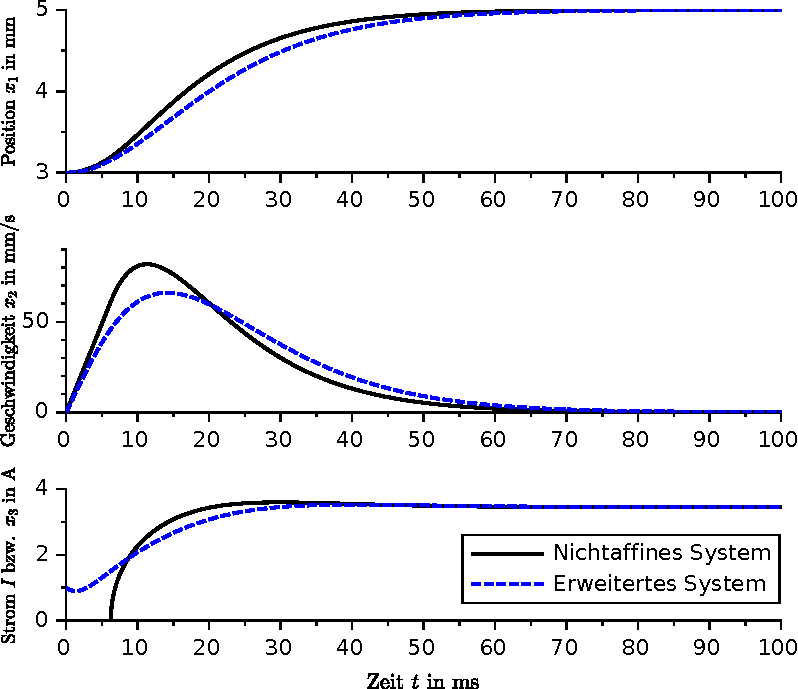
\includegraphics[width=0.85\textwidth]{Kugel_Magnet3}
\par\end{centering}
\caption{Simulation der lagegeregelten Kugel aus den Beispielen~\ref{exa:Kugel-Magnetfeld}
und~\ref{exa:Kugel-Magnetfeld-erweitert}\label{fig:Kugel-Magnet-Simulation-erweitert}}
\end{figure}


\subsection{Byrnes-Isidori-Normalform}

Gegeben sei ein nicht eingangsaffines System~(\ref{eq:Ausgangssystem-nichtaffine-mit-ausgang}).
Dieses System kann immer dargestellt werden in der Form 
\begin{equation}
\dot{x}=F(x,u)=f(x)+\sum_{i=1}^{m}g_{i}(x)\cdot\sigma_{i}(x,u)\label{eq:Vektorfeld-quasi-affin-m}
\end{equation}
mit eingangsunabhängigen Vektorfeldern $f,g_{1},\ldots,g_{m}:\mathcal{M}\to\R^{n}$
und eingangsabhängigen Skalarfeldern $\sigma_{1},\ldots,\sigma_{m}:\mathcal{M}\times\mathcal{U}\to\R$.
Eine solche Darstellung erhält man beispielsweise für $m=n$, indem
man das Vektorfeld~$F$ bezüglich der kanonischen Basis entwickelt:
\[
F(x,u)=F_{1}(x,u)\frac{\partial}{\partial x_{1}}+\cdots+F_{n}(x,u)\frac{\partial}{\partial x_{n}}.
\]

Bei den nachfolgenden Betrachtungen steht die Frage im Vordergrund,
ob die Darstellung~(\ref{eq:Vektorfeld-quasi-affin-m}) für $m=1$
möglich ist. In diesem Fall würde sich das System~(\ref{eq:Ausgangssystem-nichtaffine-mit-ausgang})
in die Form
\begin{equation}
\dot{x}=F(x,u)=f(x)+g(x)\,\sigma(x,u)\label{eq:Vektorfeld-quasi-affin-1}
\end{equation}
zerlegen lassen. Diese Zerlegung ist unter folgenden Bedingungen möglich~\cite{gruenbacher2005}:
\begin{lemma}
\label{lem:umwandlung-nicht-affin-in-quasi-affine}Ein System~(\ref{eq:Ausgangssystem-nichtaffine-mit-ausgang})
kann genau dann für Werte~$u$ aus einer Umgebung von $u_{0}\in\mathcal{U}$
in die Form~(\ref{eq:Vektorfeld-quasi-affin-1}) mit 
\begin{equation}
\left.\frac{\partial\sigma(x,u)}{\partial u}\right|_{u=u_{0}}\neq0\label{eq:quasiaffin-SF-partielle-Abl-u}
\end{equation}
zerlegt werden, wenn das Gleichungssystem
\begin{equation}
F(x,u)-F(x,u_{0})=\left.\frac{\partial F(x,u)}{\partial u}\right|_{u=u_{0}}\cdot\sigma(x,u)\label{eq:bedingung-lin-gls-quasi-affin}
\end{equation}
bezüglich~$\sigma$ lösbar ist. Die Vektorfelder aus Gl.~(\ref{eq:Vektorfeld-quasi-affin-1})
ergeben sich dabei aus
\begin{equation}
f(x)=F(x,u_{0})\quad\text{und}\quad g(x)=\left.\frac{\partial F(x,u)}{\partial u}\right|_{u=u_{0}}.\label{eq:Vektorfelder-f-g-fuer-quasi-affin}
\end{equation}
\end{lemma}
\begin{svmultproof2}
\notwendig\ Gleichungssystem~(\ref{eq:bedingung-lin-gls-quasi-affin})
habe eine Lösung~$\sigma$. Dann ergibt sich die Form~(\ref{eq:Vektorfeld-quasi-affin-1})
unmittelbar aus Gl.~(\ref{eq:Vektorfelder-f-g-fuer-quasi-affin}).

\hinreichend\ System~(\ref{eq:Ausgangssystem-nichtaffine-mit-ausgang})
sei in die Form~(\ref{eq:Vektorfeld-quasi-affin-1}) zerlegbar. Dann
gilt einerseits
\begin{equation}
F(x,u)-F(x,u_{0})=g(x)\cdot\left(\sigma(x,u)-\sigma(x,u_{0})\right),\label{eq:beweis-quasi-affine-t1}
\end{equation}
andererseits 
\begin{equation}
\left.\frac{\partial F(x,u)}{\partial u}\right|_{u=u_{0}}=\left.\frac{\partial}{\partial u}\left(g(x)\,\sigma(x,u)\right)\right|_{u=u_{0}}=g(x)\left.\frac{\partial\sigma(x,u)}{\partial u}\right|_{u=u_{0}}.\label{eq:beweis-quasi-affine-t2}
\end{equation}
Die Vektorfelder~(\ref{eq:beweis-quasi-affine-t1}) und~(\ref{eq:beweis-quasi-affine-t2})
zeigen beide in Richtung des Vektorfeldes~$g$. Wegen $\tfrac{\partial\sigma(x,u)}{\partial u}|_{u=u_{0}}\neq0$
gilt $(F(x,u)-F(x,u_{0}))\in\spann\{g(x)\}$, so dass das (bezüglich~$\sigma$
lineare) Gls.~(\ref{eq:bedingung-lin-gls-quasi-affin}) lösbar ist.
\end{svmultproof2}

In Gl.~(\ref{eq:Vektorfeld-quasi-affin-1}) kann der Eingang nur
in Richtung des von~$u$ unabhängigen Vektorfeldes~$g$ wirken.
In Verbindung mit Gl.~(\ref{eq:beweis-quasi-affine-t2}) bedeutet
das, dass zwar das Vektorfeld $\tfrac{\partial}{\partial u}F(x,u)$
von~$u$ abhängen darf, nicht aber die davon aufgespannte Distribution
$\Delta_{u}:=\im\tfrac{\partial}{\partial u}F(x,u)$.

\begin{example}
\label{exa:Kugel-Magnet-quasi-affine}Man betrachte die im Magnetfeld
schwebende Kugel aus Beispiel~\ref{exa:Kugel-Magnetfeld} mit dem
Eingang $u=I$. Für eine Entwicklungsstelle $u_{0}=I_{0}$ nimmt Gls.~(\ref{eq:bedingung-lin-gls-quasi-affin})
die Form
\[
\left(\begin{array}{c}
0\\
\frac{\rho}{m}\frac{\left(I_{0}^{2}-I^{2}\right)}{(x_{1}+s_{0})^{2}}
\end{array}\right)=\left(\begin{array}{c}
0\\
-2\frac{\rho}{m}\frac{I_{0}^{2}}{(x_{1}+s_{0})^{2}}
\end{array}\right)\cdot\sigma(x,I)
\]
an. Dieses Gleichungssystem ist für $I_{0}\neq0$ lösbar mit $\sigma(I)=-(I_{0}^{2}-I^{2})/(2I_{0})$.
Das zugehörige System~(\ref{eq:Vektorfeld-quasi-affin-1}) lautet
damit 
\[
\dot{x}=\left(\begin{array}{c}
x_{2}\\
g-\frac{\rho}{m}\frac{I_{0}^{2}}{(x_{1}+s_{0})^{2}}
\end{array}\right)+\left(\begin{array}{c}
0\\
-2\frac{\rho}{m}\frac{I_{0}}{(x_{1}+s_{0})^{2}}
\end{array}\right)\cdot\sigma(x,I).
\]
\end{example}

\begin{example}
\label{exa:raumflugkoerper}Wir betrachten einen Raumflugkörper, der
sich außerhalb der Atmosphäre um die Erde bewegt~\cite[S.~193]{nijmeijer90}.
Die Position des Flugkörpers sei in kartesischen Koordinaten durch
$x_{s}=r\cos\theta$ und $y_{s}=r\sin\theta$ mit dem Abstand~$r$
vom Erdmittelpunkt und dem Winkel~$\theta$ gegeben (Abb.~\ref{fig:Raumflugkoerper}).
Daraus ergibt sich die kinetische Energie
\[
T=\frac{m}{2}\left(\dot{x}_{s}^{2}+\dot{y}_{s}^{2}\right)=\frac{m}{2}\left(\dot{r}^{2}+r^{2}\dot{\theta}^{2}\right).
\]
Unter Berücksichtigung des Zentralpotentials erhält man die Lagrange-Funktion
\[
L=\frac{m}{2}\left(\dot{r}^{2}+r^{2}\dot{\theta}^{2}\right)+\frac{mgR^{2}}{r}
\]
mit dem Erdradius~$R$ und der Fallbeschleunigung~$g$ an der Erdoberfläche.
Der Antrieb erzeugt eine konstante Schubkraft~$\digamma$ und ist
über den Winkel~$u$ zu beeinflussen. Daraus ergibt sich folgende
Bewegungsgleichung:
\[
\left(\begin{array}{cc}
m & 0\\
0 & mr^{2}
\end{array}\right)\left(\begin{array}{c}
\ddot{r}\\
\ddot{\theta}
\end{array}\right)+\left(\begin{array}{c}
\frac{mgR^{2}}{r^{2}}-\dot{\theta}^{2}mr\\
2mr\dot{r}\dot{\theta}
\end{array}\right)=\left(\begin{array}{c}
\digamma\cos u\\
\digamma r\sin u
\end{array}\right).
\]
Mit dem Zustand $x=(r,\theta,\dot{r},\dot{\theta})^{T}$ erhält man
das Modell
\begin{equation}
\dot{x}=\left(\begin{array}{c}
x_{3}\\
x_{4}\\
-\frac{gR^{2}}{x_{1}^{2}}+x_{1}x_{4}^{2}+\frac{\digamma}{m}\cos u\\
-2\frac{x_{3}x_{4}}{x_{1}}+\frac{\digamma}{mx_{1}}\sin u
\end{array}\right).\label{eq:Rakete-nichtaffin}
\end{equation}

Es ist zu untersuchen, ob das System~(\ref{eq:Rakete-nichtaffin})
in die Form~(\ref{eq:Vektorfeld-quasi-affin-1}) zerlegt werden kann.
Gls.~(\ref{eq:bedingung-lin-gls-quasi-affin}) hat für $u$ die Form
\[
\left(\begin{array}{c}
0\\
0\\
\frac{\digamma}{m}\left(\cos u-\cos u_{0}\right)\\
\frac{\digamma}{mx_{1}}\left(\sin u-\sin u_{0}\right)
\end{array}\right)=\left(\begin{array}{c}
0\\
0\\
-\frac{\digamma}{m}\sin u_{0}\\
\frac{\digamma}{mx_{1}}\cos u_{0}
\end{array}\right)\cdot\sigma(x,u).
\]
Dieses Gleichungssystem ist in einer Umgebung von~$u_{0}$ nicht
lösbar. Damit gibt es für dieses System keine Darstellung der Form~(\ref{eq:Vektorfeld-quasi-affin-1}).
\end{example}
\begin{figure}
\begin{centering}
\resizebox{0.45\textwidth}{!}{\input{Rakete.pdftex_t}}
\par\end{centering}
\caption{Raumflugkörper außerhalb der Erdatmosphäre\label{fig:Raumflugkoerper}}
\end{figure}

Bei wohldefiniertem relativen Grad (im Sinne von Def.~\ref{def:relativer-Grad-nichtaffine-SISO})
lässt sich ein nicht eingangsaffines System~(\ref{eq:Ausgangssystem-nichtaffine-mit-ausgang})
immer in die Eingangs-Ausgangs-Normalform~(\ref{eq:Eingangs-Ausgangs-NF-nichtaffin})
überführen (Satz~\ref{thm:EA-Form-nicht-affin}). Dabei kann der
Eingang auch im zweiten Teilsystem auftreten. Hängt das zweite Teilsystem
dagegen nicht explizit vom Eingang ab, so geht die Eingangs-Ausgangs-Normalform~(\ref{eq:Eingangs-Ausgangs-NF-nichtaffin})
in die Byrnes-Isidori-Normalform\index{Byrnes-Isidori-Normalform}\index{Normalform!Byrnes-Isidori-}
\begin{equation}
\begin{array}{lcl}
\dot{\xi}_{1} & = & \xi_{2}\\
 & \vdots\\
\dot{\xi}_{r-1} & = & \xi_{r}\\
\dot{\xi}_{r} & = & a(\xi,\eta,u),\quad\text{mit}\quad\frac{\partial}{\partial u}a(\xi,\eta,u)\neq0\\
\dot{\eta}_{r+1} & = & q_{1}(\xi,\eta)\\
 & \vdots\\
\dot{\eta}_{n} & = & q_{n-r}(\xi,\eta)\\
y & = & \xi_{1}
\end{array}\label{eq:BINF-nichtaffin}
\end{equation}
über. Der nächste Satz gibt Auskunft über die Existenzbedingungen
der zugehörigen Transformation:
\begin{theorem}
\label{thm:Bynres-Isidori-nichtaffin}System~(\ref{eq:Ausgangssystem-nichtaffine-mit-ausgang})
habe an der Stelle $(p,u_{0})\in\mathcal{M}\times\mathcal{U}$ den
relativen Grad $r<n$. Das System kann genau dann mit einer Zustandstransformation
in die Byrnes-Isidori-Normalform überführt werden, wenn es in der
Form~(\ref{eq:Vektorfeld-quasi-affin-1}) darstellbar ist.
\end{theorem}
\begin{svmultproof2}
\hinreichend\ System~(\ref{eq:Ausgangssystem-nichtaffine-mit-ausgang})
sei mit $(\xi,\eta)=\Phi(x)$ in die Byrnes-Isidori-Normal\-form~(\ref{eq:BINF-nichtaffin})
transformierbar. Der Eingang~$u$ tritt dann nur in der $r$-ten
Differentialgleichung auf. Die Rücktransformation liefert unmittelbar
die Form~(\ref{eq:Vektorfeld-quasi-affin-1}) mit 
\[
g(x):=\left(\Phi^{\prime}(x)\right)^{-1}\frac{\partial}{\partial\xi_{r}}\quad\text{und}\quad\sigma(x,u):=\alpha(\xi,\eta,u)\quad\text{für}\quad x=\Phi^{-1}(\xi,\eta).
\]

\notwendig\ System~(\ref{eq:Ausgangssystem-nichtaffine-mit-ausgang})
sei in die Form~(\ref{eq:Vektorfeld-quasi-affin-1}) zerlegbar. Bei
wohldefiniertem Grad~$r$ des Systems~(\ref{eq:Ausgangssystem-nichtaffine-mit-ausgang})
im Sinne von Def.~\ref{def:relativer-Grad-nichtaffine-SISO} gilt
\[
\frac{\partial L_{F}^{r-1}h(x,u)}{\partial u}\equiv0\quad\Rightarrow\quad L_{F}^{r-1}h(x,u)=L_{F}^{r-1}h(x)=L_{f}^{r-1}h(x,u)
\]
und
\[
\begin{array}{lcl}
L_{F}^{r}h(x,u) & = & \d L_{F}^{r-1}h(x)\cdot F(x,u)\\
 & = & \d L_{f}^{r-1}h(x)\cdot\left(f(x)+g(x)\cdot\sigma(x,u)\right)\\
 & = & L_{f}^{r}h(x)+L_{g}L_{f}^{r-1}h(x)\cdot\sigma(x,u).
\end{array}
\]
Wegen $\tfrac{\partial}{\partial u}L_{F}^{r}h(x,u)=L_{g}L_{f}^{r-1}h(x)\tfrac{\partial}{\partial u}\sigma(x,u)$
ist damit auch für das sich aus~(\ref{eq:Vektorfeld-quasi-affin-1})
mit dem virtuellen Eingang $\bar{u}:=\sigma(x,u)$ ergebende eingangsaffine
System der relative Grad~$r$ im Sinne von Def.~\ref{def:relativer-Grad-SISO}
wohldefiniert. Dieses System kann in die Byrnes-Isidori-Normalform
überführt werden (Satz~\ref{thm:Byrnes-Isidori-Normalform}). Der
Eingang~$\bar{u}$ tritt nur im ersten Teilsystem auf. Mit dem Einsetzen
von $\sigma(x,u)$ bleibt die Struktur unverändert.
\end{svmultproof2}

\begin{example}
\label{exa:raumflugkoerper-byrnes-isidori}Für den Raumflugkörper
aus Beispiel~\ref{exa:raumflugkoerper} werde der Abstand zum Erdmittelpunkt
als Ausgang gewählt, d.\,h. $y=h(x)=x_{1}$. Der Eingang tritt erstmals
in der zweiten Zeitableitung des Ausgangs auf:
\[
\begin{array}{lclcl}
\dot{y} & = & \dot{x}_{1} & = & x_{3}\\
\ddot{y} & = & \dot{x}_{3} & = & -\frac{gR^{2}}{x_{1}^{2}}+x_{1}x_{4}^{2}+\frac{\digamma}{m}\cos u
\end{array}
\]
Wegen $\partial\ddot{y}/\partial u=-\tfrac{\digamma}{m}\sin u$ ist
der relative Grad $r=2$ für $u\neq i\pi$ mit $i\in\Z$ wohldefiniert.
Da das System nicht in die Form~(\ref{eq:Vektorfeld-quasi-affin-1})
zerlegt werden kann, kann es auch nicht in die Byrnes-Isidori-Normalform
transformiert werden.
\end{example}

Geht man von einem nicht eingangsaffinen Originalsystem~(\ref{eq:Ausgangssystem-nichtaffine-mit-ausgang})
zu dem erweiterten (eingangsaffinen) System~(\ref{eq:nichtaffin-erweitertes-System})
über, so existiert bei wohldefiniertem relativen Grad immer die Byrnes-isidori-Normalform
(Satz~\ref{thm:Byrnes-Isidori-Normalform}). Die zugehörige Koordinatentransformation
des erweiterten Systems~(\ref{eq:nichtaffin-erweitertes-System})
hängt aber nicht nur vom Zustand des Originalsystems~(\ref{eq:Ausgangssystem-nichtaffine-mit-ausgang}),
sondern auch vom Eingang ab.

Wenn der Eingang auf der rechten Seite des zweiten Teilsystems der
Eingangs-Ausgangs-Normalform~(\ref{thm:EA-Form-nicht-affin}) nicht
vollständig zu beseitigen ist kann man zumindest versuchen, den Einfluss
des Eingangs auf dieses Teilsystem zu reduzieren. Durch eine geeignete
Koordinatenwahl lässt sich die Anzahl der Differentialgleichungen
des zweiten Teilsystems, die direkt vom Eingang abhängen, minimieren:

\begin{proposition}
\label{prop:Auftreten-des-Eingangs-EA-NF}System~(\ref{eq:Ausgangssystem-nichtaffine-mit-ausgang})
habe an der Stelle $(p,u_{0})\in\mathcal{M}\times\mathcal{U}$ den
relativen Grad $r<n$. Unter Nutzung der Darstellung~(\ref{eq:Vektorfeld-quasi-affin-m})
habe der involutive Abschluss der von den Eingangsvektorfeldern $g_{1},\ldots,g_{m}$
aufgespannten Distribution in einer Umgebung des Punktes~$p$ die
Dimension 
\[
k:=\dim\inv\left(\spann\{g_{1},\ldots,g_{m}\}\right).
\]
Dann kann die Transformation des Systems in die Eingangs-Ausgangs-Normalform
so gewählt werden, dass der Eingang~$u$ nur in $k-1$ Differentialgleichungen
des zweiten Teilsystems auftritt.
\end{proposition}
\begin{proofsketch}Die Distribution $\Delta:=\inv(\spann\{g_{1},\ldots,g_{m}\}$
ist laut Annahme regulär und involutiv. Dann exisitieren eine Umgebung
$\mathcal{U}\subseteq\mathcal{M}$ von~$p$ und $n-k$ Skalarfelder
$\lambda_{1},\ldots,\lambda_{n-k}:\mathcal{U}\to\R$, so dass die
zugehörigen Gradienten $\d\lambda_{1},\ldots,\d\lambda_{n-k}$ den
Annihilator~$\Delta^{\perp}$ aufspannen. Die Skalarfelder $\lambda_{1},\ldots,\lambda_{n-k}$
kann man durch weitere Skalarfelder $\lambda_{n-k+1},\ldots,\lambda_{n}$
zu einer Koordinatentransformation $z=\lambda(x)$ mit $z_{i}=\lambda_{i}(x)$
für $i=1,\ldots,n$ ergänzen (Korollar~\ref{cor:ergaenzung-einer-kodistribution-integrierbar}).
Mit der Zugehörigkeit der ersten $n-k$ Funktionen zum Annihilator~$\Delta^{\perp}$
gilt $\langle\d\lambda_{i},g\rangle=L_{g}\lambda_{i}=0$ für $i=1,\ldots,n-k$
und alle $g\in\Delta$. Die verbleibenden $k$ Funktionen gehören
nicht zum Annihilator, so dass $\langle\d\lambda_{i},g\rangle=L_{g}\lambda_{i}\neq0$
für $i=n-k+1,\ldots,n$. Jeder Term $L_{g}\lambda_{i}\neq0$ führt
dazu, dass der Eingang~$u$ in der $i$-ten Gleichung der transformieten
Koordinaten auftritt.

Bei einem relativen Grad~$r$ existiert die Eingangs-Ausgangs-Normalform~(\ref{eq:Eingangs-Ausgangs-NF-nichtaffin}).
Der Eingang tritt im ersten Teilsystem in genau einer (nämlich der
letzten) Zeile auf. Durch passende Koordinatenwahl tritt der Eingang
im zweiten Teilsystem nur noch in $k-1$ Gleichungen in Erscheinung.\end{proofsketch}
\begin{example}
\label{exa:raumflugkoerper-EA-NF-reduziert}Betrachtet werde der Raumflugkörper
aus Beispiel~\ref{exa:raumflugkoerper} mit dem Ausgang aus Beispiel~\ref{exa:raumflugkoerper-byrnes-isidori}.
Das System kann in die Form~(\ref{eq:Vektorfeld-quasi-affin-m})
mit
\[
\dot{x}=F(x,u)=\underbrace{\left(\begin{array}{c}
x_{3}\\
x_{4}\\
-\frac{gR^{2}}{x_{1}^{2}}+x_{1}x_{4}^{2}\\
-2\frac{x_{3}x_{4}}{x_{1}}
\end{array}\right)}_{{\displaystyle f(x)}}+\underbrace{\left(\begin{array}{c}
0\\
0\\
\frac{\digamma}{m}\\
0
\end{array}\right)}_{{\displaystyle g}_{1}(x)}\cos u+\underbrace{\left(\begin{array}{c}
0\\
0\\
0\\
\frac{\digamma}{mx_{1}}
\end{array}\right)}_{{\displaystyle g}_{2}(x)}\sin u
\]
zerlegt werden. Die Distribution $\Delta=\spann\{g_{1},g_{2}\}$ ist
für $x_{1}\neq0$ definiert und mit $[g_{1},g_{2}]=0$ involutiv (d.\,h.
$\Delta=\inv(\Delta)$). Damit gilt $k=2$. Die Koordinaten lassen
sich so wählen, dass der Eingang nur in $k-1=1$ mal im zweiten Teilsystem
auftritt. Mit einer Umbenennung der Zustandskomponenten überführt
man~(\ref{eq:Rakete-nichtaffin}) in die Eingangs-Ausgangs-Normalform
\[
\begin{array}{lcl}
\dot{\xi}_{1} & = & \xi_{2}\\
\dot{\xi}_{2} & = & -\frac{gR^{2}}{\xi_{1}^{2}}+\xi_{1}\eta_{2}^{2}+\frac{\digamma}{m}\cos u\\
\dot{\eta}_{1} & = & \eta_{2}\\
\dot{\eta}_{2} & = & -2\frac{\xi_{2}\eta_{2}}{\xi_{1}}+\frac{\digamma}{m\xi_{1}}\sin u\\
y & = & \xi_{1}.
\end{array}
\]
Wie erwartet tritt der Eingang nur in einer der beiden Differentialgleichung
des zweiten Teilsystems auf.
\end{example}

\subsection{Eingangs-Zustands-Linearisierung und Regelungsnormalform}

In Analogie zu Abschnitt~\ref{sec:Exakte-Eingangs-Zustands-Linearisierung}
nennen wir ein nicht eingangsaffines System
\begin{equation}
\dot{x}=F(x,u)\label{eq:Ausgangssystem-nichtaffine-ohne-ausgang}
\end{equation}
mit dem eingangsabhängigen Vektorfelder $F:\mathcal{M}\times\mathcal{U}\to\R^{n}$
\emph{eingangs-zustands-linearisierbar}\index{eingangs-zustands-linearisierbar},
wenn ein Skalarfeld $h:\mathcal{M}\to\R$ exisitert, mit welchem das
resultierende System~(\ref{eq:Ausgangssystem-nichtaffine-mit-ausgang})
den relativen Grad~$n$ besitzt. In diesem Fall ist die zugehörigen
Eingangs-Ausgangs-Normalform~(\ref{eq:Eingangs-Ausgangs-NF-nichtaffin})
gleichzeitig die Regelungsnormalform\index{Regelungsnormalform}\index{Normalform!Regelungs-}
\begin{equation}
\begin{array}{lcl}
\dot{\xi}_{1} & = & \xi_{2}\\
 & \vdots\\
\dot{\xi}_{n-1} & = & \xi_{n}\\
\dot{\xi}_{n} & = & a(\xi,u),\quad\text{mit}\quad\frac{\partial}{\partial u}a(\xi,u)\neq0\\
y & = & \xi_{1}
\end{array}\label{eq:Regelungs-NF-nichtaffin}
\end{equation}
 des nicht eingangsaffinen Systems~(\ref{eq:Ausgangssystem-nichtaffine-mit-ausgang}).

\begin{theorem}
\label{thm:EZ-Linearisierung-nichtaffin}Wir betrachten System~(\ref{eq:Ausgangssystem-nichtaffine-ohne-ausgang})
in einer Umgebung von $(p,u^{0})\in\mathcal{M}\times\mathcal{U}$.
Dann sind folgende Aussagen äquivalent:
\begin{enumerate}
\item \label{enu:EZL-nichtaffin1}System~(\ref{eq:Ausgangssystem-nichtaffine-ohne-ausgang})
ist eingangs-zustands-linearisierbar.
\item \label{enu:EZL-nichtaffin2}System~(\ref{eq:Ausgangssystem-nichtaffine-ohne-ausgang})
kann in die Form~(\ref{eq:Vektorfeld-quasi-affin-1}) mit~(\ref{eq:quasiaffin-SF-partielle-Abl-u})
zerlegt werden und das aus den Vektorfeldern~$f$ und~$g$ resultierende
eingangsaffine Ersatz\-system
\begin{equation}
\dot{x}=f(x)+g(x)\bar{u}\label{eq:affines-ersatzsystem-nach-zerlegung}
\end{equation}
ist eingangs-zustands-linearisierbar.
\item \label{enu:EZL-nichtaffin3}Das erweiterte System~(\ref{eq:nichtaffin-erweitertes-System2})
ist eingangs-zustands-linearisierbar.
\end{enumerate}
\end{theorem}

\begin{svmultproof2}
(1)~$\Rightarrow$~(2): System~(\ref{eq:Ausgangssystem-nichtaffine-ohne-ausgang})
sei eingangs-zustands-linearisierbar, d.\,h. es gibt einen Diffeomorphismus
$\xi=\Phi(x)$, der System~(\ref{eq:Ausgangssystem-nichtaffine-ohne-ausgang})
in die Regelungsnormalform~(\ref{eq:Regelungs-NF-nichtaffin}) überführt.
Das transformierte System~(\ref{eq:Regelungs-NF-nichtaffin}) liegt
bereits in der Form~(\ref{eq:Vektorfeld-quasi-affin-1}) vor. Die
Zerlegung~(\ref{eq:Vektorfeld-quasi-affin-1}) ergibt sich in den
Originalkoordinaten aus 
\[
g(x):=\left(\Phi^{\prime}(x)\right)^{-1}\frac{\partial}{\partial\xi_{n}}\quad\text{und}\quad\sigma(x,u):=\alpha(\xi,u)\quad\text{für}\quad x=\Phi^{-1}(\xi),
\]
vgl. Beweis von Satz~\ref{thm:EA-Form-nicht-affin}. Mit der angegebenen
Festlegung des Eingangsvektorfeldes ist zugehörige Ersatzsystem~(\ref{eq:affines-ersatzsystem-nach-zerlegung})
eingangs-zustands-linearisierbar, da in den durch die Transformation~$\Phi$
induzierten Koordinaten die spezielle Regelungsnormalform~(\ref{eq:regelungsnormalform-eingeschraenkt})
vorliegt.

(2)~$\Rightarrow$~(1): Das System liege in der Form~(\ref{eq:Vektorfeld-quasi-affin-1})
vor und das zugehörige Ersatzsystem~(\ref{eq:affines-ersatzsystem-nach-zerlegung})
sei eingangs-zustands-linarisierbar. Die Transformation des Ersatzsystems
in die (eingangsaffine) Regelungsnormalform~(\ref{eq:Regelungsnormalform})
und Einsetzen von $\bar{u}=\sigma(x,u)$ liefert die Regelungsnormalform~(\ref{eq:Regelungs-NF-nichtaffin}),
wobei sich $\frac{\partial}{\partial u}a(\xi,u)\neq0$ aus~(\ref{eq:quasiaffin-SF-partielle-Abl-u})
ergibt. Das nicht eingangsaffine System~(\ref{eq:Ausgangssystem-nichtaffine-ohne-ausgang})
ist also eingangs-zustands-linearisierbar.

(1)~$\Rightarrow$~(3): System~(\ref{eq:Ausgangssystem-nichtaffine-ohne-ausgang})
sei mit $\xi=\Phi(x)$ in die Regelungsnormalform~(\ref{eq:Regelungs-NF-nichtaffin})
überführbar. Bedingt durch $\frac{\partial}{\partial u}a(\xi,u)\neq0$
kann insbesondere auch die Nichtlinearität~$\alpha$ (zumindest lokal)
mit $\alpha(\xi,u)\stackrel{!}{=}v$ kompensiert werden (Satz über
die Umkehrfunktion). Die Ableitung 
\[
\dot{v}=\underbrace{\frac{\partial}{\partial\xi}a(\xi,u)\dot{\xi}}_{{\displaystyle \tilde{\alpha}(\xi,v)}}+\underbrace{\frac{\partial}{\partial u}a(\xi,u)}_{{\displaystyle \tilde{\beta}(\xi,v)}}\dot{u}
\]
führt mit $\dot{u}=\tilde{u}$ auf die Regelungsnormalform 
\[
\begin{array}{lcl}
\dot{\xi}_{1} & = & \xi_{2}\\
 & \vdots\\
\dot{\xi}_{n-1} & = & \xi_{n}\\
\dot{\xi}_{n} & = & v\\
\dot{v} & = & \tilde{\alpha}(\xi,v)+\tilde{\beta}(\xi,v)\tilde{u}.
\end{array}
\]
des erweiterten Systems~(\ref{eq:nichtaffin-erweitertes-System2}).
Die Transformation des erweiterten Systems~(\ref{eq:nichtaffin-erweitertes-System2})
wird durch
\[
\tilde{\Phi}:\quad\tilde{x}=\left(\begin{array}{c}
x\\
u
\end{array}\right)\mapsto\left(\begin{array}{c}
\xi\\
v
\end{array}\right)=\left(\begin{array}{c}
\Phi(x)\\
\alpha(\Phi(x),u)
\end{array}\right)
\]
beschrieben. Die zugehörige Jacobimatrix
\[
\tilde{\Phi}^{\prime}(\tilde{x})=\tilde{\Phi}^{\prime}(x,u)=\left(\begin{array}{cc}
\Phi^{\prime}(x) & 0\\
* & \frac{\partial}{\partial u}a(\xi,u)
\end{array}\right)
\]
ist regulär.

(3)~$\Rightarrow$~(1): Das erweiterte Systems~(\ref{eq:nichtaffin-erweitertes-System2})
sei eingangs-zustands-linearisierbar. Damit gibt es einen Ausgang~$\tilde{h}$,
für den das erweiterte System~(\ref{eq:nichtaffin-erweitertes-System2})
den relativen Grad $n+1$ besitzt. Daraus erhält man einen Ausgang~$h$
des Originalsystems~(\ref{eq:Ausgangssystem-nichtaffine-ohne-ausgang})
mit dem relativen Grad~$n$ (vgl. Prop.~\ref{prop:relativer-Grad-erweitertes-System}).
\end{svmultproof2}

Die Bedingung~\ref{enu:EZL-nichtaffin3} von Satz~\ref{thm:EZ-Linearisierung-nichtaffin}
lässt sich über Satz~\ref{thm:Exakte-Eingangs-Zustands_Linearisierung}
bzw. Satz~\ref{thm:Exakte-Eingangs-Zustands-Linearisierung-Formen}
überprüfen. Bei Bedingung~\ref{enu:EZL-nichtaffin2} ist zusätzlich
Lemma~\ref{lem:umwandlung-nicht-affin-in-quasi-affine} zu beachten.
Insbesondere wird man bei den Bedingungen~\ref{enu:EZL-nichtaffin2}
und~\ref{enu:EZL-nichtaffin3} auf eingangsaffine Vergleichssysteme~(\ref{eq:nichtaffin-erweitertes-System2})
und~(\ref{eq:Vektorfeld-quasi-affin-1}) geführt und kann damit die
in Abschnitt~\ref{sec:Exakte-Eingangs-Zustands-Linearisierung} beschriebenen
Ansätze zur Berechnung eines Ausgangs mit vollem relativen Grad nutzen.

\begin{example}
Man betrachte den Raumflugkörper aus Beispiel~\ref{exa:raumflugkoerper}.
Es wurde gezeigt, dass das System~(\ref{eq:Rakete-nichtaffin}) nicht
in die Form~(\ref{eq:Vektorfeld-quasi-affin-1}) zerlegt werden kann.
Daher ist das System auch nicht eingangs-zustands-linearisierbar.
\end{example}

\begin{example}
\label{exa:Dreirad-Modell-EZ-SISO}Wir modifizieren den zweirädrigen
mobilen Roboter aus Abschnitt~\ref{subsec:Mobiler-Roboter-Modellierung}
zu dem in Abb.~\ref{fig:dreirad} gezeigten dreirädrigen Roboter.
Der Antrieb erfolgt jetzt über die im Gleichlauf betriebenen Räder
der Hinterachse und resultiert in einer in Fahrtrichtung orientierten
Geschwindigkeit~$v$. Daraus ergibt sich die translatorische Bewegung
\begin{equation}
\begin{array}{lcl}
\dot{x}_{1} & = & v\,\sin\varphi,\\
\dot{x}_{2} & = & v\,\cos\varphi.
\end{array}\label{eq:dreirad-modell-trans}
\end{equation}
Zusätzlich kann über das erste Rad der Lenkwinkel~$\delta$ eingestellt
werden. Für das sich aus Hinterachsmittelpunkt, Vorderachse und dem
Kreismittelpunkt~$P$ ergebende rechtwinklige Dreieck gilt 
\begin{equation}
\tan\delta=\frac{D}{R},\label{dreirad-lenkwinkel}
\end{equation}
wobei~$D$ den Abstand zwischen Vorder- und Hinterachse bezeichnet.
Für die Bewegung auf der (fiktiven) Kreisbahn besteht zwischen der
translatorischen Geschwindigkeit~$v$ und der Winkelgeschwindigkeit~$\dot{\varphi}$
die Beziehung $v=R\dot{\varphi}$, womit der Kreisradius~$R$ aus
Gl.~(\ref{dreirad-lenkwinkel}) eliminiert werden kann. Mit $x_{3}=\varphi$
erhält man insgesamt das kinematische Modell
\begin{equation}
\begin{array}{lcl}
\dot{x}_{1} & = & v\,\sin x_{3},\\
\dot{x}_{2} & = & v\,\cos x_{3},\\
\dot{x}_{3} & = & \frac{v}{D}\,\tan\delta.
\end{array}\label{eq:dreirad-kinematisches-modell}
\end{equation}

\begin{figure}
\begin{centering}
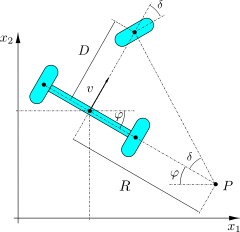
\includegraphics[width=0.48\textwidth]{Roboter_drei_Raeder}
\par\end{centering}
\caption{Mobiler Roboter in der $(x_{1},x_{2})$-Ebene\label{fig:dreirad}}
\end{figure}

Beeinflusst man den dreirädrigen Roboter nur über den Lenkwinkel~$\delta$
bei konstanter Geschwindigkeit $v>0$, so liegt mit Gl.~(\ref{eq:dreirad-kinematisches-modell})
ein nicht eingangsaffines Eingrößensystem vor, welches sich unmittelbar
in die Form~(\ref{eq:Vektorfeld-quasi-affin-1}) zerlegten lässt:
\[
\left(\begin{array}{c}
\dot{x}_{1}\\
\dot{x}_{2}\\
\dot{x}_{3}
\end{array}\right)=\underbrace{\left(\begin{array}{c}
v\,\sin x_{3}\\
v\,\cos x_{3}\\
0
\end{array}\right)}_{{\displaystyle f(x)}}+\underbrace{\left(\begin{array}{c}
0\\
0\\
\frac{v}{D}
\end{array}\right)}_{{\displaystyle g(x)}}\cdot\tan\delta.
\]
Die Vektorfelder~$f$ und~$g$ stimmen bis auf jeweils einen konstanten
Faktor mit den entsprechenden Vektorfeldern des mobilen Roboters überein.
In Beispiel~\ref{exa:Roboter-eingangs-zustands-linearisierung} wurde
gezeigt, dass das zugehörige System nicht eingangs-zustands-linearisierbar
ist. Gemäß Satz~\ref{thm:EZ-Linearisierung-nichtaffin} ist damit
auch das nichtaffine Modell~(\ref{eq:dreirad-kinematisches-modell})
in der hier betrachteten Eingangskonstellation nicht eingangs-zustands-linearisierbar.
\end{example}

\section{Flache Systeme\label{sec:Flache-Systeme}}

\subsection{Definition und Einführungsbeispiele}

Mit der Formulierung des Flachheitsbegriffs im Kontext der Regelungstheorie
gelang es Mitte der neunziger Jahre der Forschergruppe um Michel Fliess
einen mathematischen Rahmen zu schaffen, der den systematischen Entwurf
von Steuerung und Regelung für eine große Klasse nichtlinearer Systeme
ermöglicht~\cite{FLMR95ijc}. Eine zentrale Größe bei dieser Herangehensweise
ist der sog. flache Ausgang, der eine integralfreie Parametrierung
aller Systemgrößen ermöglicht.

Unsere Betrachtungen beschränken sich auf Zustandsraummodelle der
Form 
\begin{equation}
\dot{x}=F(x,u)\label{eq:Ausgangssystem-Flachheit-MIMO}
\end{equation}
mit einem hinreichend glatten eingangsabhängigen Vektorfeld $F:\mathcal{M}\times\mathcal{U}\to\R^{n}$,
das auf einer offenen Teilmenge $\mathcal{M}\subseteq\R^{n}$ und
einer weiteren Teilmenge $\mathcal{U}\subseteq\R^{m}$ definiert ist.
Für diese Systemklasse lässt sich der die Flachheit wie folgt definieren~\cite{rudolph2003habil}:
\begin{definition}
\label{def:flach}Das System~(\ref{eq:Ausgangssystem-Flachheit-MIMO})
heißt \emph{(differentiell) flach}\index{flach}, wenn es ein $m$-Tupel
$\zeta:=(\zeta_{1},\ldots,\zeta_{m})^{T}$ sowie glatte Funktionen~$\Psi,\Theta$
gibt, so dass
\begin{enumerate}
\item \label{enu:flach1}$x=\Psi(\zeta,\dot{\zeta},\ldots,\zeta^{(n_{x})})$
mit $n_{x}<\infty$ und
\item \label{enu:flach2}$u=\Theta(\zeta,\dot{\zeta},\ldots,\zeta^{(n_{u})})$
mit $n_{u}<\infty$.
\end{enumerate}
Dann heißt~$\zeta$ \emph{flacher Ausgang}.
\end{definition}

Die Existenz eines flachen Ausgangs nach Def.~\ref{def:flach} bedeutet,
dass die in Gl.~(\ref{eq:Ausgangssystem-Flachheit-MIMO}) auftretenden
Systemgrößen, nämlich der Zustand~$x$ und der Eingang~$u$, eindeutig
aus dem Verlauf des flachen Ausgangs~$\zeta$ und einer endlichen
Anzahl von Zeitableitungen bestimmt werden können. Man spricht dabei
auch von einer integralfreien Parametrierung aller Systemgrößen, da
zur Bestimmung der Systemgrößen keine Integration im Sinne des Lösens
von Differentialgleichungen erforderlich ist. Bei der Definition der
Flachheit wird zusätzlich oft die differentielle Unabhängigkeit der
Komponenten~$\zeta_{i}$ des Tupels~$\zeta$ gefordert. Diese Forderung
ist hier nicht nötig~\cite{fliess1999}. Allerdings muss die Dimension
des flachen Ausgangs~$\zeta$ mit der Dimension des Eingangsvektors~$u$
übereinstimmen.

In der Regel werden die in Def.~\ref{def:flach} angegebenen Abbildungen~$\Psi$
und~$\Theta$ nicht global für alle Werte von $(\zeta,\dot{\zeta},\ddot{\zeta},\ldots)$
definiert sein. Sind diese Abbdilungen auf einer offenen und nicht
leeren Teilmenge definiert, dann nennt man das System~(\ref{eq:Ausgangssystem-Flachheit-MIMO})
\emph{lokal flach} bzw. spricht von einem \emph{lokal flachen Ausgang}~\cite{levine2007equivalence,levine2011}.
Da bei praxisrelevanten Systemen die entsprechenden Abbildungen nahezu
immer Ausnahmepunkte (Singularitäten) besitzen, werden wir die Begriffe
flach und lokal flach synonym verwenden.

Der flache Ausgang muss nicht notwendigerweise mit dem technischen
Ausgang dieses Systems übereinstimmen. Vielmehr ist der flache Ausgang
eine Hilfsgröße, die für den Entwurf einer Steuerung bzw. einer Regelung
hilfreich ist. Bei Eingrößensystemen sind die Existenzbedingungen
für einen flachen Ausgang bekannt (siehe Abschnitt~\ref{subsec:Flacher-nichtflacher-Ausgang}).
Im Mehrgrößenfall ist der Test eines Systems auf Flachheit bzw. die
Berechnung eines flachen Ausgangs trotz zahlreicher theoretischer
Fortschritte bisher nicht abschließend gelöst~\cite{levine2011,schoeberl2012at,verhoeven2013,franke2014diss,fritzsche2016at}. 

In vielen Anwendungsfällen ergibt sich der flache Ausgang aus der
Regelungsaufgabe bzw. besitzt eine physikalische Bedeutung. Diese
Situation wird zunächst an einem Eingrößensystem illustriert~\cite{sira-ramirez2002converter,gensior2006}:

\begin{example}
\label{exa:Hochsetzsteller-flach}Das gemittelte Modell des in Abschnitt~\ref{subsec:Hochsetzsteller-Modellierung}
beschriebenen Hochsetzstellers
\begin{equation}
\begin{array}{lcl}
\dot{x}_{1} & = & -(1-u)\frac{1}{L}x_{2}+\frac{E}{L}\\
\dot{x}_{2} & = & (1-u)\frac{1}{C}x_{1}-\frac{1}{RC}x_{2}
\end{array}\label{eq:hochsetzsteller-system-flachheit}
\end{equation}
besitzt den flachen Ausgang
\begin{equation}
\zeta=\frac{L}{2}x_{1}^{2}+\frac{C}{2}x_{2}^{2}.\label{eq:hochsetz-y}
\end{equation}
Physikalisch ist diese Größe als die in der Spule und im Kondensator
gespeicherte elektrische Energie zu verstehen. Die zeitliche Ableitung
des flachen Ausgangs~(\ref{eq:hochsetz-y}) vereinfacht sich unter
Einsetzen der Systemdynamik~(\ref{eq:hochsetzsteller-system-flachheit})
zu
\begin{equation}
\begin{array}{rcl}
\dot{\zeta} & = & Lx_{1}\dot{x}_{1}+Cx_{2}\dot{x}_{2}\\
 & = & Ex_{1}-\frac{1}{R}x_{2}^{2}.
\end{array}\label{eq:hochsetz-dy}
\end{equation}
Durch Eliminination der Variablen~$x_{2}$ aus den Gleichungen~(\ref{eq:hochsetz-y})
und~(\ref{eq:hochsetz-dy}) erhält man die erste Zustandsvariable
\begin{equation}
x_{1}=\psi_{1}(\zeta,\dot{\zeta})=\sqrt{\frac{R^{2}C^{2}E^{2}}{4L^{2}}+\frac{2}{L}\zeta+\frac{RC}{L}\dot{\zeta}}-\frac{RCE}{2L},\label{eq:hochsetz-flach-x1}
\end{equation}
unter Ausnutzung dieses Zwischenergebnisses in Verbindung mit~(\ref{eq:hochsetz-dy})
die zweite Zustandsvariable:
\begin{equation}
x_{2}=\psi_{2}(\zeta,\dot{\zeta})=\sqrt{R\left(E\psi_{1}(\zeta,\dot{\zeta})-\dot{\zeta}\right)}.\label{eq:hochsetz-flach-x2}
\end{equation}
Der Eingang tritt in der zweiten Zeitableitung des flachen Ausgangs
auf:
\begin{equation}
\begin{array}{rcl}
\ddot{\zeta} & = & E\dot{x}_{1}-\frac{2}{R}x_{2}\dot{x}_{2}\\
 & = & \frac{E}{L}\left(E+(u-1)x_{2}\right)+\frac{2}{RC}x_{2}\left((u-1)x_{1}+\frac{1}{R}x_{2}\right).
\end{array}\label{eq:hochsetz-ddy}
\end{equation}
Durch Umstellen nach~$u$ und Einsetzen von~(\ref{eq:hochsetz-flach-x1})
und~(\ref{eq:hochsetz-flach-x2}) erhält man die Parametrierung
\[
\begin{array}{cll}
u & = & 1-\frac{R^{2}C\left(E^{2}-L\ddot{\zeta}\right)+2Lx_{2}^{2}}{Rx_{2}\left(RCE+2Lx_{1}\right)}\\
 & = & 1-\frac{R^{2}C\left(E^{2}-L\ddot{\zeta}\right)+2L\psi_{2}^{2}(\zeta,\dot{\zeta})}{R\psi_{2}(\zeta,\dot{\zeta})\left(RCE+2L\psi_{1}(\zeta,\dot{\zeta})\right)}.\\
 & =: & \Theta(\zeta,\dot{\zeta},\ddot{\zeta})
\end{array}
\]
des Eingangs.
\end{example}

Im nächsten Beispiel wird ein Mehrgrößensystem betrachtet~\cite{rothfuss97flach,ryu2011}:
\begin{example}
\label{exa:Mobiler-Roboter-Flachheit}Man betrachte das kinematische
Modell
\begin{equation}
\dot{x}=\left(\begin{array}{c}
\sin x_{3}\\
\cos x_{3}\\
0
\end{array}\right)u_{1}+\left(\begin{array}{c}
0\\
0\\
1
\end{array}\right)u_{2}\label{eq:mobiler-roboter-MIMO-modell-flachheit}
\end{equation}
des mobilen Roboters aus Abschnitt~\ref{subsec:Mobiler-Roboter-Modellierung}
mit den Eingängen~$u_{1}$ und~$u_{2}$. Es wird nachfolgend gezeigt,
dass die Position des Roboters in der Ebene einen flachen Ausgang
darstellt, also $\zeta=(\zeta_{1},\zeta_{2})^{T}=(x_{1},x_{2})^{T}$.
Aus dem Quotienten der ersten beiden Differentialgleichungen~(\ref{eq:mobiler-roboter-MIMO-modell-flachheit})
ergibt sich 
\[
\frac{\dot{x}_{1}}{\dot{x}_{2}}=\frac{\sin x_{3}}{\cos x_{3}}=\tan x_{3}\quad\text{bzw.}\quad x_{3}=\arctan\left(\frac{\dot{x}_{1}}{\dot{x}_{2}}\right).
\]
Damit erhält man die Abbildung~$\Psi$ aus Bedingung~\ref{enu:flach1}
von Def.~\ref{def:flach}:
\[
x=\Psi(\zeta,\dot{\zeta})=\left(\begin{array}{c}
\zeta_{1}\\
\zeta_{2}\\
\arctan\frac{\dot{\zeta}_{1}}{\dot{\zeta}_{2}}
\end{array}\right).
\]
Aus der Summe der Quadrate der ersten zwei Systemgleichungen 
\[
\dot{x}_{1}^{2}+\dot{x}_{2}^{2}=u_{1}^{2}\sin^{2}x_{3}+u_{1}^{2}\cos^{2}x_{3}=u_{1}^{2}
\]
erhält man die Parametrierung
\[
u_{1}=\theta_{1}(\zeta,\dot{\zeta})=\pm\sqrt{\dot{\zeta}_{1}^{2}+\dot{\zeta}_{2}^{2}}
\]
des ersten Eingangs, aus der dritten Systemgleichung ergibt sich die
Parametrierung des zweiten Eingangs: 
\[
\begin{array}{lll}
u_{2} & = & \dot{x}_{3}\\
 & = & \frac{\d}{\d t}\arctan\frac{\dot{x}_{1}}{\dot{x}_{2}}\\
 & = & \left.\frac{\dot{z}}{1+z^{2}}\right|_{z=\dot{\zeta}_{1}/\dot{\zeta}_{2}}\\
 & = & \frac{\ddot{\zeta}_{1}\dot{\zeta}_{2}-\dot{\zeta}_{1}\ddot{\zeta}_{2}}{\dot{\zeta}_{1}^{2}+\dot{\zeta}_{2}^{2}}\\
 & =: & \theta_{2}(\zeta,\dot{\zeta},\ddot{\zeta}).
\end{array}
\]
Damit liegt eine vollständige Parametrierung aller Systemgrößen vor.
\end{example}

\subsection{Zusammenhang zwischen flachem Ausgang und Systemausgang für Eingrößensysteme\label{subsec:Flacher-nichtflacher-Ausgang}}

Man betrachte System~(\ref{eq:Ausgangssystem-Flachheit-MIMO}) mit
$m=1$, d.\,h. wir beschränken uns in diesem Abschnitt auf Systeme
mit einem (skalarwertigen) Eingang. Die Flachheit eines derartigen
Eingrößensystems lässt sich folgendermaßen charakterisieren~\cite{nieuwstadt1994}:
\begin{theorem}
\label{thm:flach-EZ-lin-SISO}Ein Eingrößensystem~(\ref{eq:Ausgangssystem-Flachheit-MIMO})
ist genau dann (lokal) flach, wenn es (lokal) exakt eingangs-zustands-linearisierbar
ist. Ein flacher Ausgang hat den relativen Grad~$n$.
\end{theorem}
\begin{svmultproof2}
\notwendig\ System~(\ref{eq:Ausgangssystem-Flachheit-MIMO}) sei
exakt eingangs-zustands-linearisierbar, d.\,h. es existiert eine
Ausgangsabbildung $h:\mathcal{M}\to\R$, für die das System den relativen
Grad~$n$ besitzt. Wir setzen $\zeta=h(x)$. Durch den wohldefinierten
relativen Grad $r=n$ kann das System~(\ref{eq:Ausgangssystem-Flachheit-MIMO})
mit einem Diffeomorphismus $\xi=\Phi(x)$ in die Regelungsnormalform~(\ref{eq:Regelungs-NF-nichtaffin})
transformiert werden. Zwischen dem Ausgang~$\zeta$ und den Zuständen~$\xi$
bestehen folgende Beziehungen:
\[
\zeta=\xi_{1},\;\dot{\zeta}=\xi_{2},\;\ddot{\zeta}=\xi_{3},\;\ldots,\zeta^{(n-1)}=\xi_{n}.
\]
Da~$\Phi$ ein Diffeomorphismus ist, existiert die Umkehrabbildung
\[
\begin{array}{lll}
x & = & \Phi^{-1}(\xi)\\
 & = & \Phi^{-1}(\xi_{1},\xi_{2},\ldots,\xi_{n})\\
 & = & \Phi^{-1}(\zeta,\dot{\zeta},\ldots,\zeta^{(n-1)})\\
 & =: & \Psi(\zeta,\dot{\zeta},\ldots,\zeta^{(n-1)}),
\end{array}
\]
so dass Bedingung~\ref{enu:flach1} aus Def.~\ref{def:flach} erfüllt
ist. Wegen $\tfrac{\partial}{\partial u}\alpha(\xi,u)\neq0$ kann~$\alpha$
bezüglich des zweiten Arguments invertiert werden, d.\,h. es gibt
eine Umkehrabbildung~$\alpha^{-1}$ mit 
\[
u=\alpha^{-1}(\xi,\dot{\xi}_{n})=:\Theta(\zeta,\dot{\zeta},\ldots,\zeta^{(n-1)},\zeta^{(n)}).
\]
Damit ist auch Bedingung~\ref{enu:flach2} aus Def.~\ref{def:flach}
erfüllt. Der Ausgang~$\zeta$ ist folglich ein flacher Ausgang von~(\ref{eq:Ausgangssystem-Flachheit-MIMO}).

\hinreichend\ System~(\ref{eq:Ausgangssystem-Flachheit-MIMO}) sei
flach, d.\,h. es gibt einen flachen Ausgang~$\zeta$ und Abbildungen~$\Psi,\Theta$
nach Def.~\ref{def:flach}. Sei $n_{u}$ die höchste Ableitungsordnung
des flachen Ausgangs, durch welche der Eingang~$u$ direkt beeinflusst
wird. Dann kann man die Bedingung~\ref{enu:flach1} von Def.~\ref{def:flach}
lokal nach~$\zeta^{(n_{u})}$ auflösen und erhält eine Beziehung
der Form
\begin{equation}
\zeta^{(n_{u})}=\varUpsilon\left(\zeta,\dot{\zeta},\ldots,\zeta^{(n_{u}-1)},u\right).\label{eq:flache-Paramrierung-SISO-aufgeloest}
\end{equation}
Mit Gl.~(\ref{eq:flache-Paramrierung-SISO-aufgeloest}) bekommt man
eine Eingangs-Ausgangs-Beschreibung des Systems~(\ref{eq:Ausgangssystem-Flachheit-MIMO}).
Mit $z_{1}=\zeta,z_{2}=\dot{\zeta},\ldots,z_{n_{u}}=\zeta^{(n_{u}-1)}$
könnte man aus~(\ref{eq:flache-Paramrierung-SISO-aufgeloest}) eine
(eventuell nicht alle Zustände des Originalsystems~(\ref{eq:Ausgangssystem-Flachheit-MIMO})
erfassende) Zustandsbeschreibung erhalten. Aus der Darstellung~(\ref{eq:flache-Paramrierung-SISO-aufgeloest})
ergibt sich unmittelbar ein relativer Grad~$n_{u}$ (vgl. Abschnitt~\ref{subsec:Relativer-Grad-nichtaffine}).

Angenommen, es gelte $n_{u}<n$. Dann würde das System~(\ref{eq:Ausgangssystem-Flachheit-MIMO})
eine Nulldynamik der Dimension $n-n_{u}$ besitzen. Für $\zeta\equiv0$
wäre damit der Zustand nicht eindeutig festgelegt. Damit wäre Bedingung~\ref{enu:flach1}
von Def.~\ref{def:flach} verletzt, so dass~$\zeta$ kein flacher
Ausgang wäre (Widerspruch zur Annahme). Der Fall $n_{u}>n$ ist auch
für den nicht eingangsaffinen Fall analog zu Anmerkung~\ref{rem:relativer-Grad-Systemordnung}
auszuschließen. Somit muss $n_{u}=n$ gelten, d.\,h. das System~(\ref{eq:Ausgangssystem-Flachheit-MIMO})
ist eingangs-zustands-linearisierbar.
\end{svmultproof2}

Zur Überprüfung eines Eingrößensystems auf Flachheit kann man somit
die in Abschnitt~\ref{sec:Exakte-Eingangs-Zustands-Linearisierung}
angegebenen Existenzbedingungen bzw. Berechnungsverfahren heranziehen.
Basierend auf dem Beweis von Satz~\ref{thm:flach-EZ-lin-SISO} lassen
sich die in Def.~\ref{def:flach} aufgeführten endlichen Ableitungsordnungen
für Eingrößensysteme konkretisieren:
\begin{corollary}
Für ein Eingrößensystem~(\ref{eq:Ausgangssystem-Flachheit-MIMO})
gilt $n_{x}=n-1$ und $n_{u}=n$.
\end{corollary}

\begin{example}
\label{exa:inverses-pendel-gleichstrommotor-flache-param}Wir setzen
die Betrachungen zu dem inversen Pendel mit Gleichstromantrieb aus
den Beispielen~\ref{exa:inverses-pendel-gleichstrommotor} und~\ref{exa:inverses-pendel-gleichstrommotor-formen}
fort. Für die Ausgangsabbildung $h(x)=x_{1}$ hat das System den relativen
Grad~$n$. Damit ist $\zeta=h(x)=x_{1}$ ein flacher Ausgang. Die
Zeitableitungen des flachen Ausgangs lassen sich über Lie-Ableitungen
darstellen
\[
\begin{array}{cclcl}
\zeta & = & h(x) & = & x_{1}\\
\dot{\zeta} & = & L_{f}h(x) & = & x_{2}\\
\ddot{\zeta} & = & L_{f}^{2}h(x) & = & \frac{mg\ell}{J}\sin x_{1}+\frac{d}{J}x_{2}+\frac{K}{J}x_{3}
\end{array}
\]
und liefern die Parametrierung
\[
\begin{array}{lcl}
x_{1} & = & \zeta\\
x_{2} & = & \dot{\zeta}\\
x_{3} & = & \frac{d\dot{\zeta}+J\ddot{\zeta}-mg\ell\sin\zeta}{K}
\end{array}
\]
des Zustands~$x$ bezüglich des flachen Ausgangs~$\zeta$. Aus der
dritten Zeitableitung
\[
\begin{array}{lcl}
\zeta^{(3)} & = & L_{f}^{3}h(x)+L_{g}L_{f}^{2}h(x)\,u\\
 & = & -\frac{JK^{2}x_{2}+L\left(dKx_{3}-Jmg\ell x_{2}\cos x_{1}+dmg\ell\sin x_{1}-d^{2}x_{2}\right)+JKRx_{3}}{J^{2}L}+\frac{K}{JL}\,u\\
 & = & \frac{mg\ell\dot{\zeta}\cos\zeta-d\ddot{\zeta}}{J}-\frac{R}{L}\ddot{\zeta}+\frac{Rmg\ell\sin\zeta-(dR+K^{2})\dot{\zeta}}{JL}+\frac{K}{JL}\,u
\end{array}
\]
erhält man die flache Parametrierung
\[
u=\frac{K^{2}\dot{\zeta}+L\left(J\zeta^{(3)}-mg\ell\dot{\zeta}\cos\zeta+d\ddot{\zeta}\right)+R\left(J\ddot{\zeta}-mg\ell\sin\zeta+d\dot{\zeta}\right)}{K}
\]
des Eingangs.
\end{example}

Auch bei einem flachen System kann es mitunter aus anwendungsspezifischen
Gründen sinnvoll sein, zusätzlich einen nichtflachen Ausgang (z.\,B.
als Mess- oder Regelgröße) in die regelungstechnischen Betrachtungen
einzubeziehen. Zwischen diesen beiden Ausgängen besteht dann folgender
Zusammenhang~\cite{hagenmeyer2004scl}:
\begin{theorem}
Man betrachte System~(\ref{eq:Ausgangssystem-Flachheit-MIMO}) mit
einem flachen Ausgang
\begin{equation}
\zeta=\lambda(x)\label{eq:ausgang-flach}
\end{equation}
und einem nichtflachen Systemausgang
\begin{equation}
y=h(x),\label{eq:ausgang-nicht-flach}
\end{equation}
für den das System einen relativen Grad $r<n$ habe. Dann kann der
System\-ausgang~(\ref{eq:ausgang-nicht-flach}) wie folgt über den
flachen Ausgang~(\ref{eq:ausgang-flach}) parametriert werden:
\begin{equation}
y=\varrho(\zeta,\dot{\zeta},\ldots,\zeta^{(n-r)}).\label{eq:parametrierung-nichtflacher-systemausgang}
\end{equation}
\end{theorem}

\begin{svmultproof2}
Mit dem flachen Ausgang~(\ref{eq:ausgang-flach}) hat das System
den relativen Grad~$n$ (Satz~\ref{thm:flach-EZ-lin-SISO}) und
kann in die Regelungsnormalform~(\ref{eq:Regelungs-NF-nichtaffin})
transformiert werden. Gl.~(\ref{eq:parametrierung-nichtflacher-systemausgang})
ist dann gleichbedeutend mit 
\begin{equation}
y=\varrho(\xi_{1},\xi_{2},\ldots,\xi_{n-r+1}).\label{eq:parametrierung-nichtflacher-systemausgang-xi}
\end{equation}
Die Regelungsnormalform~(\ref{eq:Regelungs-NF-nichtaffin}) werde
durch $\dot{\xi}=\bar{f}(\xi,u)$ beschrieben. Gibt man den Systemausgang
in $\xi$-Koordinaten mit $y=\bar{h}(\xi)$ an, so hängt die Lie-Ableitung
\[
L_{\bar{f}}\bar{h}(\xi,u)=\sum_{i=1}^{n}\frac{\partial\bar{h}(\xi)}{\partial\xi_{i}}\cdot\bar{f}_{i}(\xi,u)=\sum_{i=1}^{n-1}\frac{\partial\bar{h}(\xi)}{\partial\xi_{i}}\cdot\xi_{i+1}+\frac{\partial\bar{h}(\xi)}{\partial\xi_{n}}\alpha(\xi,u)
\]
genau dann vom Eingang~$u$ ab (d.\,h. $\tfrac{\partial}{\partial u}L_{\bar{f}}\bar{h}(\xi,u)\neq0$),
wenn die Abbildung~$\bar{h}$ von der letzten Komponente~$\xi_{n}$
des Zustands abhängt (d.\,h. $\partial\bar{h}(\xi)/\partial\xi_{n}\neq0$).
Dieser Fall tritt bei $r=1$ auf.

Sei jetzt $r>1$, d.\,h. $\partial\bar{h}(\xi)/\partial\xi_{n}\equiv0$.
Angenommen, die Ausgangsabbildung~$\bar{h}$ hängt nur von den ersten
$j$ Zuständen $\xi_{1},\ldots,\xi_{j}$ ab. Bei wohldefiniertem relativen
Grad haben dann der Ausgang und seine Lie-Ableitungen die Form
\begin{equation}
\begin{array}{c}
\bar{h}(\xi_{1},\ldots,\xi_{j})\\
L_{\bar{f}}\bar{h}(\xi_{1},\ldots,\xi_{j+1})\\
\vdots\\
L_{\bar{f}}^{r-1}\bar{h}(\xi_{1},\ldots,\xi_{j+r-1})\\
L_{\bar{f}}^{r}\bar{h}(\xi_{1},\ldots,\xi_{j+r};u),
\end{array}\label{eq:Lie-fuer-Hagenmeyer}
\end{equation}
so dass eine explizite Abhängigkeit vom Eingang erstmals in der $r$-ten
Lie-Ableitung auftritt. Da das Vektorfeld\,$\bar{f}$ nur in der
letzten Komponente vom Eingang abhängt, muss die vorherige Lie-Ableitung
$L_{\bar{f}}^{r-1}\bar{h}$ explizit von der letzten Zustandskomponente~$\xi_{n}$
abhängen. In der vorletzten Zeile von~(\ref{eq:Lie-fuer-Hagenmeyer})
muss dann $\xi_{j+r-1}=\xi_{n}$ bzw. $j+r-1=n$ gelten. Damit erhält
man $j=n-r+1$, d.\,h. die Ausgangsabbilldung~$\bar{h}$ hat dann
die Form (bzw. die Abhängigkeiten) wie in Gl.~(\ref{eq:parametrierung-nichtflacher-systemausgang-xi})
und damit wie in Gl.~(\ref{eq:parametrierung-nichtflacher-systemausgang})
\end{svmultproof2}


\subsection{Verallgemeinerte Regelungsnormalform\label{subsec:Verallgemeinerte-Regelungsnormalform}}

Ist~(\ref{eq:Ausgangssystem-Flachheit-MIMO}) ein Eingrößensystem
(d.\,h. $m=1$), dann kann es bei Kenntnis eines flachen Ausgangs~(\ref{eq:ausgang-nicht-flach})
in die Regelungsnormalform~(\ref{eq:Regelungs-NF-nichtaffin}) überführt
werden. In Verbindung mit einem nichtflachen Systemausgang~(\ref{eq:ausgang-nicht-flach}),
für den das System einen wohldefinierten relativen Grad aufweist,
wäre eine Transformation in die Eingangs-Ausgangs- oder Byrnes-Isidori-Normalform
möglich. Diese Normalformen beruhen auf Zustandstransformationen.
Die nachfolgend eingeführte Normalform erfordert dagegen eine eingangsabhängige
und damit zeitvariante Transformation.

Man betrachte ein differentiell flaches Eingrößensystem~(\ref{eq:Ausgangssystem-Flachheit-MIMO}),
welches mit dem Systemausgang~(\ref{eq:ausgang-nicht-flach}) den
relativen Grad $r<n$ besitzt. Die ersten $r$ Komponenten der Transformation~$\Phi$
werden --- wie bei Eingangs-Ausgangs- oder Byrnes-Isidori-Normalform
--- über die ersten $r$ Lie-Ableitungen und somit über den Ausgang~$y$
und seine Zeitableitungen bis zur Ordnung $r-1$ definiert:
\begin{equation}
\begin{array}{lclcl}
y & = & \phi_{1}(x) & = & h(x)\\
\dot{y} & = & \phi_{2}(x) & = & L_{f}h(x)\\
 & \vdots &  & \vdots\\
y^{(r-1)} & = & \phi_{r}(x) & = & L_{f}^{r-1}h(x)
\end{array}\label{eq:transf-verallg-RNF1}
\end{equation}
Die $r$-te Lie-Ableitung, die mit der Zeitableitung der Ordnung~$r$
des Ausgangs übereinstimmt, hängt vom Eingang~$u$ ab:
\begin{equation}
y^{(r)}=L_{f}^{r}h(x,u).\label{eq:yr-verallg-RNF}
\end{equation}
Davon ausgehend definieren wir unter Hinzunahme weiterer Zeitableitungen
die verbleibenden $n-r$ Komponenten von~$\Phi$:
\begin{equation}
\begin{array}{lcl}
y^{(r)} & =: & \phi_{r}(x,u)\\
y^{(r+1)} & =: & \phi_{r+1}(x,u,\dot{u})\\
 & \vdots\\
y^{(n-1)} & =: & \phi_{n}(x,u,\dot{u},\ldots,u^{(n-r-1)}).
\end{array}\label{eq:transf-verallg-RNF2}
\end{equation}
Mit~(\ref{eq:transf-verallg-RNF1}) und~(\ref{eq:transf-verallg-RNF2})
erhält man eine Abbildung 
\[
z=\Phi(x,u,\dot{u},\ldots,u^{(n-r-1)}),
\]
mit der man unter entsprechenden Regularitätsannahmen das System~(\ref{eq:Ausgangssystem-Flachheit-MIMO})
in die \emph{verallgemeinerte Regelungsnormalform}\index{verallgemeinerte Regelungsnormalform}\index{Normalform!verallgemeinerte Regelungs-}
(eng. \emph{generalized controller canonical form}) überführt~\cite{fliess1990}:
\begin{equation}
\begin{array}{lcl}
\dot{z}_{1} & = & z_{2}\\
 & \vdots\\
\dot{z}_{n-1} & = & z_{n}\\
\dot{z}_{n} & = & \delta(z,u,\dot{u},\ldots,u^{(n-r)})\\
y & = & z_{1}.
\end{array}\label{eq:verallgemeinerte-Regelungsnormalform}
\end{equation}
Im Unterschied zur klassischen Zustandsraumdarstellung~(\ref{eq:Ausgangssystem-Flachheit-MIMO})
treten neben dem Eingang~$u$ auch Zeitalbeitungen $\dot{u},\ddot{u},\ldots$
auf. Zur Unterscheidung spricht man dann auch von einer \emph{verallgemeinerten
Zustandsraumdarstellung} und einem \emph{verallgemeinerten Zustand}~$z$.

Die Linearisierung 
\begin{equation}
\bar{a}_{0}=-\frac{\partial\delta}{\partial z_{1}},\ldots,\bar{a}_{n-1}=-\frac{\partial\delta}{\partial z_{n}},\quad\bar{b}_{0}=\frac{\partial\delta}{\partial u},\ldots,\bar{b}_{n-r}=\frac{\partial\delta}{\partial u^{(n-r)}}\label{eq:koeff-linearisierung-verallg-RNF}
\end{equation}
von~(\ref{eq:verallgemeinerte-Regelungsnormalform}) im Arbeitspunkt
$z=0$, $u=0,\ldots,u^{(n-r)}=0$ führt mit $y=z_{1},\,\dot{y}=z_{2},\ldots,y^{(n-1)}=z_{n}$
auf die Differentialgleichung
\[
y^{(n)}+\bar{a}_{n-1}y^{(n-1)}+\cdots+\bar{a}_{1}\dot{y}+\alpha_{0}y=\bar{b}_{n-r}u^{(n-r)}+\cdots+\bar{b}_{1}\dot{u}+\bar{b}_{0}u
\]
bzw. im Laplace-Bereich auf die Übertragungsfunktion 
\begin{equation}
G(s)=\frac{Y(s)}{U(s)}=\frac{\bar{b}_{n-r}s^{n-r}+\cdots+\bar{b}_{1}s+\bar{b}_{0}}{s^{n}+\bar{a}_{n-1}s^{n-1}+\cdots+\bar{a}_{1}s+\bar{a}_{0}}.\label{eq:flach-vRNF-UF}
\end{equation}
Ein Vergleich mit der Übertragungsfunktion~(\ref{eq:rel-grad-UF1})
aus Anmerkung~\ref{rem:Nulldynamik-Nullstellen-Uebertragungsfunktion}
offenbart, dass das Zählerpolynom von~(\ref{eq:flach-vRNF-UF}) das
charakteristisch Polynom der (linearisierten) Nulldynamik ist.

\begin{remark}
\label{rem:Zeitableitungen-Lie-Ableitungen}Bei einem eingangsaffinen
System~(\ref{eq:Ausgangssystem-fuer-BINF}) nimmt die $r$-te Zeit\-ableitung~(\ref{eq:yr-verallg-RNF})
des Ausgangs die Form 
\[
y^{(r)}=L_{f}^{r}h(x)+L_{g}L_{f}^{r-1}h(x)u
\]
an. Die nächste Zeitableitung ergibt sich dann zu
\begin{equation}
\begin{array}{lcl}
y^{(r+1)} & = & \d L_{f}^{r}h(x)\,\dot{x}+\d L_{g}L_{f}^{r-1}h(x)\,\dot{x}\,u+L_{g}L_{f}^{r-1}h(x)\,\dot{u}\\
 & = & L_{f}^{r+1}h(x)+L_{g}L_{f}^{r}h(x)u+L_{f}L_{g}L_{f}^{r-1}h(x)u\\
 &  & +\,L_{g}^{2}L_{f}^{r-1}h(x)u^{2}+L_{g}L_{f}^{r-1}h(x)\dot{u},
\end{array}\label{eq:yr1-flach-affine-vRNF}
\end{equation}
siehe~\cite{Lamnabhi-Lagarrigue88,zhang2006feedback}. Dabei tritt
zwar ein nichtlinearer (nämlich quadratischer) Term in~$u$ auf,
die rechte Seite ist aber affin in der höchsten Zeitableitung von~$u$.
Die Berücksichtigung von Zeitableitung des Ausgang mit einer Ordnung,
die größer als der relative Grad ist, hat sich bei Systemen mit nicht
wohldefiniertem relativen Grad bewährt~\cite{leith2001}.
\end{remark}

Ähnlich wie bei der ,,klassischen`` Regelungsnormalform~(\ref{eq:Regelungsnormalform})
kann man auch bei der verallgemeinerten Regelungsnormalform~(\ref{eq:verallgemeinerte-Regelungsnormalform})
versuchen, dem System eine vorgegebene lineare Dynamik einzuprägen.
Diese Wunschdynamik beschreibt man durch die Forderung 
\[
\delta(z,u,\dot{u},\ldots,u^{(n-r)})\stackrel{!}{=}-a_{0}z_{1}-\cdots-a_{n-1}z_{n}
\]
an die letzte Differentialgleichung in~(\ref{eq:verallgemeinerte-Regelungsnormalform})
mit den Koeffizienten $a_{0},\ldots,a_{n-1}\in\R$. Diese Gleichung
ist nach der höchsten Ableitung~$u^{(n-r)}$ des Eingangs umzustellen.
Dabei erhält man einen dynamischen Regler, bei dem ausgehend von~$u^{(n-r)}$
über eine Integratorkette der Eingang~$u$ für die Regelstrecke erzeugt
wird. Diese Herangehensweise ist bei flachen Eingrößensystemen in
der Regel nicht sinnvoll, da diese Systeme auch mit einer statischen
Rückführung linearisiert bzw. stabilisiert werden können (Satz~\ref{thm:flach-EZ-lin-SISO}).
Eine Ausnahme bildet das in Abschnitt~\ref{subsec:Modellbasierte-Regelung-nichtlinear-maximalphasig}
vorgestellte Verfahren zur Regelung einer bestimmten Klasse nichtminimalphasiger
Systeme. Bei mehrvariablen System findet die verallgemeinerte Regelungsnormalform
im Zusammenhang mit der Linearisierung durch quasi-statische Rückführungen
Verwendung (vgl. Abschnitt~\ref{subsec:Quasi-statisch}). 

\begin{example}
Das Modell~(\ref{eq:system-inverses-pendel-mit-traegheitsrad}) des
inversen Pendels mit Trägheitsrad aus Beispiel~\ref{exa:Inverses-Pendel-mit-Traegheitsrad-EZ-distr}
hat für den Ausgang $y=h(x)=x_{3}$ (Geschwindigkeit des Trägheitsrads)
den relativen Grad $r=1$. Mit $\xi_{1}=x_{3}$, $\eta_{1}=x_{1}$
und $\eta_{2}=J_{1}x_{2}+I_{2}x_{3}$ überführt man das System in
die Byrnes-Isidori-Normalform 
\[
\begin{array}{lcl}
\dot{\xi}_{1} & = & -\frac{m_{0}}{J_{1}-I_{2}}\sin\eta_{1}+\frac{J_{1}}{I_{2}(J_{1}-I_{2})}\,u\\
\dot{\eta}_{1} & = & -\frac{I_{2}\xi_{1}-\eta_{2}}{J_{1}}\\
\dot{\eta}_{2} & = & m_{0}\sin\eta_{1}\\
y & = & \xi_{1}.
\end{array}
\]
Linearisiert man die Nulldynamik
\[
\begin{array}{lcl}
\dot{\eta}_{1} & = & \frac{1}{J_{1}}\eta_{2}\\
\dot{\eta}_{2} & = & m_{0}\sin\eta_{1}
\end{array}
\]
im Punkt $\eta=0$, so hat zugehörige die Jacobimatrix die Eigenwerte
$s_{1,2}=\pm\sqrt{m_{0}/J_{1}}$. Die Ruhelage $\eta=0$ ist somit
instabil, so dass das Gesamtsystem nicht minimalphasig ist.

Im Vergleich dazu wird das System nachfolgend in die verallgemeinerte
Regelungsnormalform~(\ref{eq:verallgemeinerte-Regelungsnormalform})
überführt. Die Transformation 
\[
\left.\begin{array}{lcl}
z_{1} & = & x_{3}\\
z_{2} & = & -\frac{m_{0}}{J_{1}-I_{2}}\sin x_{1}+\frac{J_{1}}{I_{2}(J_{1}-I_{2})}\,u\\
z_{3} & = & -\frac{m_{0}}{J_{1}-I_{2}}x_{2}\cos x_{1}+\frac{J_{1}}{I_{2}(J_{1}-I_{2})}\,\dot{u}
\end{array}\right\} \quad z=\Phi(x,u,\dot{u})
\]
führt auf ein System der Form
\[
\begin{array}{lcl}
\dot{z}_{1} & = & z_{2}\\
\dot{z}_{2} & = & z_{3}\\
\dot{z}_{3} & = & \delta(z,u,\dot{u},\ddot{u})\\
y & = & z_{1}.
\end{array}
\]
Die Funktion~$\alpha$ besteht aus einem vergleichsweise umfangreichen
Ausdruck. Die Linearisierung in $z=0,\,u=0,\ldots,\,\ddot{u}=0$ liefert
entsprechend Gl.~(\ref{eq:koeff-linearisierung-verallg-RNF}) die
Koeffizienten
\[
\bar{b}_{0}=\left.\frac{\partial\delta}{\partial u}\right|_{0}=-\frac{m_{0}}{I_{2}(J_{1}-I_{2})},\;\bar{b}_{1}=\left.\frac{\partial\delta}{\partial\dot{u}}\right|_{0}=0,\;\bar{b}_{2}=\left.\frac{\partial\delta}{\partial\ddot{u}}\right|_{0}=\frac{J_{1}}{I_{2}(J_{1}-I_{2})}.
\]
Daraus erhält man das Zählerpolynom der Übertragungsfunktion~(\ref{eq:flach-vRNF-UF}).
Die Nullstellen $s_{1,2}=\pm\sqrt{m_{0}/J_{1}}$ stimmen mit den oben
berechneten Eigenwerten der linearisierten Nulldynamik überein.
\end{example}

\section{Mehrvariable Systeme\label{sec:Mehrvariable-Systeme}}

Die Methode der exakten Linearisierung durch Rückführung wird in diesem
Abschnitt auf Mehrgrößensysteme erweitert~\cite[Kapitel~5]{isidori3},
\cite[Abschnitt~{6.5.2}]{kwatny2000}.

\subsection{Vektorieller relativer Grad\label{subsec:Vektorieller-relativer-Grad}}

Man betrachte ein Mehrgrößensystem mit $m$ Ein- bzw. Ausgängen $u_{1},\ldots,u_{m}$
und $y_{1},\ldots,y_{m}$. Das System habe die eingangsaffine Form
\begin{equation}
\dot{x}=f(x)+\sum_{j=1}^{m}g_{j}(x)\,u_{j},\quad y=h(x)\label{eq:MIMO-eingangsaffin}
\end{equation}
mit Vektorfeldern $f,g_{1},\ldots,g_{m}:\mathcal{M}\to\R^{n}$ und
einer offenen Teilmenge $\mathcal{M}\subseteq\R^{n}$. Die vektorielle
Abbildung $h:\mathcal{M}\to\R^{m}$ fasst die $m$ Skalarfelder $h_{1},\ldots,h_{m}:\mathcal{M}\to\R$
mit $h=(h_{1},\ldots,h_{m})^{T}$ zusammen. Alle Felder seien hinreichend
glatt. 

\begin{definition}
\label{def:relativer-Grad-MIMO}Das System~(\ref{eq:MIMO-eingangsaffin})
hat an der Stelle $p\in\mathcal{M}$ den \emph{(vektoriellen) relativen
Grad} $(r_{1},\ldots,r_{m})$ (engl. \emph{vector relative degree})\index{relativer Grad!vektorieller},
falls

\begin{enumerate}
\item $L_{g_{j}}L_{f}^{k}h_{i}(x)=0$ für alle $x$ aus einer Umgebung von~$p$
sowie für alle $i,j\in\{1,\ldots,m\}$ und $k\in\{0,\ldots,r-2\}$,
und
\item die Matrix
\[
\Lambda(x)=\left(\begin{array}{ccc}
L_{g_{1}}L_{f}^{r_{1}-1}h_{1}(x) & \cdots & L_{g_{m}}L_{f}^{r_{1}-1}h_{1}(x)\\
\vdots & \ddots & \vdots\\
L_{g_{1}}L_{f}^{r_{m}-1}h_{m}(x) & \cdots & L_{g_{m}}L_{f}^{r_{m}-1}h_{m}(x)
\end{array}\right)
\]
im Punkt $x=p$ regulär ist.
\end{enumerate}
\end{definition}

Zur Bestimmung der Komponente~$r_{i}$ des vektoriellen relativen
Grads würde man vom Ausgang~$y_{i}$ solange Zeitableitungen bilden,
bis mindestens ein Eingang explizit auftritt:
\[
\begin{array}{lcl}
y_{i} & = & h_{i}(x)\\
\dot{y}_{i} & = & L_{f}h_{i}(x)\\
 & \vdots\\
y_{i}^{(r_{i}-1)} & = & L_{f}^{r_{i}-1}h_{i}(x)\\
y_{i}^{(r_{i})} & = & L_{f}^{r_{i}}h_{i}(x)+L_{g_{1}}L_{f}^{r_{i}-1}h_{i}(x)\,u_{1}+\cdots+L_{g_{m}}L_{f}^{r_{i}-1}h_{i}(x)\,u_{m}.
\end{array}
\]
Führt man dieses Schema für $r_{1},\ldots,r_{m}$ durch und fasst
die jeweils letzten Zeilen zusammen, so erhält man für das (zustandsabhängige)
Eingangs-Ausgangs-Verhalten die Beschreibung
\begin{equation}
\left(\begin{array}{c}
y_{1}^{(r_{1})}\\
\vdots\\
y_{m}^{(r_{m})}
\end{array}\right)\!=\!\underbrace{\left(\begin{array}{c}
L_{f}^{r_{1}}h_{1}(x)\\
\vdots\\
L_{f}^{r_{m}}h_{m}(x)
\end{array}\right)}_{{\displaystyle \Gamma(x)}}\!+\!\underbrace{\left(\begin{array}{ccc}
L_{g_{1}}L_{f}^{r_{1}-1}h_{1}(x) & \cdots & L_{g_{m}}L_{f}^{r_{1}-1}h_{1}(x)\\
\vdots & \ddots & \vdots\\
L_{g_{1}}L_{f}^{r_{m}-1}h_{m}(x) & \cdots & L_{g_{m}}L_{f}^{r_{m}-1}h_{m}(x)
\end{array}\right)}_{{\displaystyle \Lambda(x)}}\!\!\left(\begin{array}{c}
u_{1}\\
\vdots\\
u_{m}
\end{array}\right).\label{eq:MIMO-E-A-Beschreibung}
\end{equation}

Die zwischen den Ein- und Ausgängen auftretenden nichtlinearen Verkopplungen
lassen sich mit der Einführung des virtuellen Eingangsvektors $v=(v_{1},\ldots,v_{m})^{T}$
entsprechend
\begin{equation}
\Gamma(x)+\Lambda(x)u\stackrel{!}{=}v\quad\Longrightarrow\quad u=\Lambda^{-1}(x)\cdot\left(v-\Gamma(x)\right)\label{eq:entkopplung-mimo}
\end{equation}
durch eine statische Zustandsrückführung\index{Rückführung!statische}
kompensieren. Systeme mit wohldefiniertem relativen Grad nennt man
daher \emph{(statisch) eingangs-ausgangs-linearisierbar}.\index{eingangs-ausgangs-linearisierbar!statisch}
Die Matrix~$\Lambda$ heißt in diesem Zusammenhang auch \emph{Entkopplungsmatrix}\index{Entkopplungsmatrix}. 

Das Eingangs-Ausgangs-Verhalten wird nach der Entkopplung durch $m$
Integratorketten der Längen $r_{1},\ldots,r_{m}$ beschrieben: 
\[
y_{1}^{(r_{1})}=v_{1},\ldots,y_{m}^{(r_{m})}=v_{m}.
\]
Damit erhält man $m$ steuerbare lineare Teilsysteme, die durch 
\begin{equation}
\begin{array}{ccl}
v_{i} & = & -a_{i,0}(y_{i}-w_{i})-a_{i,1}\dot{y}_{i}-\cdots-a_{i,r_{i}-1}y^{(r_{i}-1)}\\
 & = & -a_{i,0}(h_{i}(x)-w_{i})-a_{i,1}L_{f}h_{i}(x)-\cdots-a_{i,r_{i}-1}L_{f}^{r_{i}-1}h_{i}(x)
\end{array}\label{eq:stabilisierung-mimo-teilsysteme}
\end{equation}
für $i=1,\ldots,m$ bezüglich des Sollwertvektors $w=(w_{1},\ldots,w_{m})^{T}$
stabilisiert werden können. Die Koeffizienten~$a_{i,j}$ sind dabei
so zu wählen, dass für jedes Teilsystem~$i$ das charakteristische
Polynom
\[
a_{i,0}+a_{i,1}s+\cdots+a_{i,r_{i}-1}s^{r_{i}-1}+s^{r_{i}}
\]
ein Hurwitz-Polynom ist.

\begin{example}
\label{exa:Zweigelenkmanipulator}Abb.~\ref{fig:Zweigelenkmanipulator}
zeigt einen Zweigelenkmanipulator. Der Vektor~$q$ enthält die die
Konfiguration beschreibenden Winkel~$q_{1}$ und~$q_{2}$. Der Manipulator
stimmt weitgehend mit dem Acrobot aus Beispiel~\ref{exa:Acrobot-max-rel-grad}
überein, so dass man die Massenmatrix~(\ref{eq:acrobot-M}) und der
Vektor~(\ref{eq:acrobot-C}) der Zentrifugal- und Corioliskräfte
übernehmen kann. Im Unterschied zum Acrobot wird der Manipulator in
der horizontalen Ebene, also senkrecht zum Schwerefeld, betrieben.
Dadurch treten keine Potentialkräfte auf. Zusätzlich verfügt der Manipulator
über zwei Stelleingriffe, nämlich die in den Gelenken eingeprägten
Drehmomente $\tau=(\tau_{1},\tau_{2})^{T}$. Die Bewegungsgleichungen
haben dann die Form
\begin{equation}
M(q)\ddot{q}+C(q,\dot{q})=\tau.\label{eq:mani-euler-lagrange}
\end{equation}

Definiert man die Winkelgeschwindigkeiten $v:=\dot{q}$, als Hilfsgrößen,
so erhält man aus der Bewegungsgleichung das Zustandsraummodell
\begin{equation}
\left(\begin{array}{c}
\dot{q}\\
\dot{v}
\end{array}\right)=\left(\begin{array}{c}
v\\
-M^{-1}(q)\,C(q,v)
\end{array}\right)+\left(\begin{array}{c}
0\\
M^{-1}(q)
\end{array}\right)u\label{eq:mani-zustandsdarstellung}
\end{equation}
mit dem Zustand $x=(q^{T},v^{T})^{T}=(q_{1},q_{2},\dot{q}_{1},\dot{q}_{2})^{T}$
und dem Eingang $u=\tau$. Als Ausgang verwenden wir die Konfigurationsvariablen,
d.\,h. 
\begin{equation}
y=q=\left(\begin{array}{c}
q_{1}\\
q_{2}
\end{array}\right)=\left(\begin{array}{c}
x_{1}\\
x_{2}
\end{array}\right).\label{eq:y-q-mani}
\end{equation}
Die erste Zeitableitung 
\begin{equation}
\dot{y}=\dot{q}=v\label{eq:dy-v-mani}
\end{equation}
hängt nicht direkt vom Eingang~$u$ ab. Aus der zweiten Zeitableitung
\[
\ddot{y}=\dot{v}=-M^{-1}(q)\,C(q,v)+M^{-1}(q)\,u
\]
liest man unmittelbar
\[
\Gamma(x)=-M^{-1}(q)\,C(q,v)\quad\text{und}\quad\Lambda(x)=M^{-1}(q)
\]
ab. Aufgrund der Regularität der Massenmatrix existiert die Entkopplungsmatrix~$\Lambda$
und ist regulär. Damit besitzt das System den relativen Grad $r=(2,2)$.
Mit Gl.~(\ref{eq:entkopplung-mimo}) kompensiert man die Nichtlinearitäten
und entkoppelt gleichzeitig die zwei Teilsysteme. Das System geht
dadurch in zwei Integratorketten der Länge $r_{1}=r_{2}=2$ über,
die mit Gl.~(\ref{eq:stabilisierung-mimo-teilsysteme}) stabilisiert
werden können. Dabei gibt man für jedes der Teilsysteme $i=1,2$ ein
charakteristisches Polynom $a_{i,0}+a_{i,1}s+s^{2}$ mit den Koeffizienten
$a_{i,0},a_{i,1}>0$ vor. Die stabilisierende Rückführung 
\[
\begin{array}{lcl}
u & = & -\Lambda^{-1}(x)\cdot\left(\left(\begin{array}{c}
a_{1,0}(x_{1}-w_{1})+a_{1,1,}x_{3}\\
a_{2,0}(x_{2}-w_{2})+a_{2,1}x_{4}
\end{array}\right)+\Gamma(x)\right)\\
 & = & C(q,\dot{q})-M(q)\cdot\left(\begin{array}{c}
a_{1,0}(q_{1}-w_{1})+a_{1,1,}\dot{q}_{1}\\
a_{2,0}(q_{2}-w_{2})+a_{1,2,}\dot{q}_{2}
\end{array}\right)
\end{array}
\]
für eine Sollposition $w=(w_{1},w_{2})^{T}$ stellt bezüglich des
Zustands\-raum\-modells~(\ref{eq:mani-zustandsdarstellung}) eine
statische Rückführung dar. Andererseits erfolgt die Stabilisierung
über eine Linearkombination des Ausgangs~(\ref{eq:y-q-mani}) und
seiner Zeit\-ableitung~(\ref{eq:dy-v-mani}). Daher kann man die
Rückführung auch als einen PD-Regler\index{PD-Regler} auffassen.
\end{example}
\begin{figure}
\begin{centering}
\resizebox{0.45\textwidth}{!}{\input{mani-voll.pdftex_t}}
\par\end{centering}
\caption{Ebener Zweigelenkmanipulator\label{fig:Zweigelenkmanipulator}}
\end{figure}

\begin{remark}
\label{rem:Mechanisch-relativer-grad}Man betrachte ein mechanisches
System, welches durch Euler-Lagrange-Gleichungen zweiter Art (wie
z.\,B. Gl.~(\ref{eq:mani-euler-lagrange})) beschrieben wird. Wählt
man als einen Eingang eine Kraft bzw. ein Moment und als Ausgang eine
davon direkt beeinflusste verallgemeinerte Position, dann führt --
bedingt durch das zweite Newtonsche Axiom (siehe~\cite{nolting1})
-- eine Eingangs-Ausgangs-Linearisierung zu einem relativen Grad~$2$.
Für ein Mehr\-größen\-system, bei welchem man die verallgemeinerten
Koordinaten~$q$ als Ausgang wählt und für jeden mechanischen Freiheitsgrad
ein unabhängiger Stelleingriff zur Verfügung steht\footnote{Mechanische Systeme, bei denen für jeden mechanischen Freiheitsgrad
ein Stelleingriff zur Verfügung steht, nennt man \emph{vollständig
direkt gesteuert} oder \emph{vollständig aktuiert}.}, erhält man mit der gleichen Überlegung einen vektoriellen relativen
Grad $(2,\ldots,2)$. 

Bezüglich der Bewegungsgleichung~(\ref{eq:mani-euler-lagrange})
kann man die durch die Gln.~(\ref{eq:entkopplung-mimo}) und~(\ref{eq:stabilisierung-mimo-teilsysteme})
beschriebene Rückführung in der Form
\begin{equation}
\tau=C(q,\dot{q})-M(q)\cdot\left(K_{P}(q-w)+K_{D}\dot{q}\right)\label{eq:berechnetes-moment}
\end{equation}
mit der vektoriellen Führungsgröße~$w$ angeben. Die Matrizen~$K_{P}$
und~$K_{D}$ beschreiben den P- bzw. D-Anteil der Reglerverstärkung
und sind üblicherweise Diagonal\-matrizen
\[
\begin{array}{lcl}
K_{P} & = & \diag\left(a_{1,0},\ldots,a_{m,0}\right),\\
K_{D} & = & \diag\left(a_{1,1},\ldots,a_{m,1}\right),
\end{array}
\]
vgl. Gl.~(\ref{eq:stabilisierung-mimo-teilsysteme}). Das rückgeführte
System geht bei Linksmultiplikation mit der inversen Massenmatrix
in ein lineares Differentialgleichungsystem über:
\[
\begin{array}{lrcl}
 & M(q)\left(\ddot{q}+K_{D}\dot{q}+K_{P}q\right) & = & M(q)K_{P}w\\
\Longleftrightarrow & \ddot{q}+K_{D}\dot{q}+K_{P}q & = & K_{P}w
\end{array}
\]
\end{remark}
Die sehr einfache Form~(\ref{eq:berechnetes-moment}) der Rückführung,
mit der man auch den Übergang zum Zustandsraummodell~(\ref{eq:mani-zustandsdarstellung})
aussparen kann, ist an die Verwendung des Vektors~$q$ der verallgemeinerten
Positionen als Systemausgang gebunden. Bei Verwendung eines anderen
Ausgangs erhält man in der Regel eine kompliziertere Rückführung.

\begin{example}
\label{exa:Zweigelenkmanipulator-kartesisch}Zu dem Manipulator aus
Beispiel~\ref{exa:Zweigelenkmanipulator} betrachten wir einen neuen
Ausgang, der die Position des Endeffektors in kartesischen Koordinaten
beschreibt:
\[
y=h(x)=\left(\begin{array}{c}
h_{1}(x)\\
h_{2}(x)
\end{array}\right)=\left(\begin{array}{c}
l_{1}\cos x_{1}+l_{2}\cos(x_{1}+x_{2})\\
l_{1}\sin x_{1}+l_{2}\sin(x_{1}+x_{2})
\end{array}\right).
\]
Auch hierzu ist der relative Grad zu bestimmen. In der ersten Zeitableitung
des Ausgangs
\[
\dot{y}=\left(\begin{array}{c}
-l_{1}x_{3}\sin x_{1}-l_{2}(x_{3}+x_{4})\sin(x_{1}+x_{2})\\
\phantom{+}l_{1}x_{3}\cos x_{1}+l_{2}(x_{3}+x_{4})\cos(x_{1}+x_{2})
\end{array}\right)
\]
treten die Eingänge nicht auf. Als zweite Zeitableitung erhält man
einen vergleichsweise umfangreichen Ausdruck, auf dessen Wiedergabe
hier verzichtet wird. Allerdings treten in dieser Ableitung beide
Eingänge auf. Die Entkopplungsmatrix~$\Lambda$ besitzt die Determinante
\[
\det\Lambda(x)=\frac{2l_{1}l_{2}\sin x_{2}}{2a_{1}a_{2}-a_{3}(1+\cos(2x_{2}))^{2}}.
\]

Die Entkoplungsmatrix ist folglich für $x_{2}=0,\pm\pi,\pm2\pi,\ldots$
singulär, so dass an diesen Stellen der relative Grad $r=(2,2)$ nicht
wohldefiniert ist. Dabei ist zu beachten, dass jede in kartesischen
Koordinaten beschriebene Position des Endeffektors im Bereich $0<\|y\|_{2}<l_{1}+l_{2}$
durch zwei verschiedene Gelenkwinkel eingestellt werden kann. Der
Übergang von einer Variante der Gelenkwinkel auf die andere würde
das Durchlaufen einer der o.\,g. Singularitäten erfordern. Für $a_{3}>2a_{1}a_{2}$
können in Abhängigkeit vom Winkel~$x_{2}$ zusätzlich Singularitäten
auftreten.
\end{example}

Bei wohldefiniertem relativen Grad kann das System~(\ref{eq:MIMO-eingangsaffin})
immer in die Eingangs-Ausgangs-Normalform transformiert werden:
\begin{theorem}
\label{thm:EA-NF-MIMO}System~(\ref{eq:MIMO-eingangsaffin}) habe
im Punkt $p\in\mathcal{M}$ den relativen Grad $(r_{1},\ldots,r_{m})$.
Wir setzen
\begin{equation}
\begin{array}{lccclclcccl}
z_{1,1} & = & \phi_{1,1}(x) & = & h_{1}(x), & \ldots, & z_{m,1} & = & \phi_{m,1}(x) & = & h_{m}(x),\\
z_{1,2} & = & \phi_{1,2}(x) & = & L_{f}h_{1}(x), & \ldots, & z_{m,2} & = & \phi_{m,2}(x) & = & L_{f}h_{m}(x),\\
 & \vdots &  & \vdots &  &  &  & \vdots &  & \vdots\\
z_{1,r_{1}} & = & \phi_{1,r_{1}}(x) & = & L_{f}^{r_{1}-1}h_{1}(x), & \ldots, & z_{m,r_{m}} & = & \phi_{m,r_{m}}(x) & = & L_{f}^{r_{m}-1}h_{m}(x).
\end{array}\label{eq:Trans-EA-NF-MIMO1}
\end{equation}
Ferner sei 
\begin{equation}
r:=r_{1}+\cdots+r_{m}.\label{eq:vektor-relativer-grad-summarisch}
\end{equation}
Falls $r<n$, so gibt es $n-r$ weitere Funktionen 
\begin{equation}
z_{m+1,k}=\phi_{m+1,k}(x)\quad\text{für}\quad k=1,\ldots,n-r,\label{eq:Trans-EA-NF-MIMO2}
\end{equation}
so dass die durch Zusammenfassen der Gln.~(\ref{eq:Trans-EA-NF-MIMO1})
und~(\ref{eq:Trans-EA-NF-MIMO2}) entstandene Abbildung~$\Phi$
mit $z=\Phi(x)$ in einer Umgebung von~$p$ ein lokaler Diffeomorphismus
ist, der das System~(\ref{eq:MIMO-eingangsaffin}) in die \emph{Eingangs-Ausgangs-Normalform}\index{Eingangs-Ausgangs-Normalform}\index{Normalform!Eingangs-Ausgangs-}
überführt. Diese Normalform besteht aus $m$ Teilsystemen der Form
\begin{equation}
\begin{array}{lcl}
\dot{z}_{i,1} & = & z_{i,2}\\
 & \vdots\\
\dot{z}_{i,r_{i}-1} & = & z_{i,r_{i}}\\
\dot{z}_{i,r_{i}} & = & \alpha_{i}(z)+\beta_{i,1}(z)u_{1}+\cdots+\beta_{i,m}(z)u_{m}
\end{array}\label{eq:EA-NF-MIMO1}
\end{equation}
mit 
\[
\begin{array}{lcl}
\alpha_{i}(z) & = & L_{f}^{r_{i}}h_{i}(x)\\
\beta_{i,j}(z) & = & L_{g_{j}}L_{f}^{r_{i}-1}h_{i}(x)
\end{array}
\]
für $i,j=1,\ldots,m$. Für $r<n$ gibt es ein weiteres Teilsystem
der Form
\begin{equation}
\dot{z}_{m+1,k}=q_{k}(z)+d_{k,1}(z)u_{1}+\cdots+d_{k,m}(z)u_{m}\label{eq:EA-NF-MIMO2}
\end{equation}
mit 
\[
\begin{array}{lcl}
q_{k}(z) & = & L_{f}\phi_{m+1,k}(x)\\
d_{k,j}(z) & = & L_{g_{j}}\phi_{m+1,k}(x)
\end{array}
\]
für $k=1,\ldots,n-r$ und $j=1,\ldots,m$.
\end{theorem}
\begin{proofsketch}Ähnlich wie in Lemma~\ref{lem:Lin-Unabh-Kovektoren}
kann man zeigen, dass bei wohldefiniertem relativen Grad $(r_{1},\ldots,r_{m})$
die Kovektoren
\[
\d h_{1}(p),\ldots,\d L_{f}^{r_{1}-1}h_{1}(p),\ldots,\d h_{m}(p),\ldots,\d L_{f}^{r_{m}-1}h_{m}(p)
\]
linear unabhängig sind (siehe auch~\cite[Lemma~{5.1.1}]{isidori3}).
Diese Kovektoren spannen einen $r$-dimensionalen Unterraum~$\mathbb{U}$
im Dualraum auf. Mit einer Basis $\{b_{1},\ldots,b_{n-r}\}$ des $(n-r$)-dimensionalen
\index{Annihilatorraum}Annihilatorraums~$\mathbb{U}^{\perp}$ konstruiert
man lineare Funktionale $\phi_{m+1,i}(x)=b_{i}^{T}x$, mit denen man
die Funktionen~(\ref{eq:Trans-EA-NF-MIMO1}) zu einem Diffeomorphismus
ergänzt. Die Form~(\ref{eq:EA-NF-MIMO1}) bzw.~(\ref{eq:EA-NF-MIMO2})
des transformierten Systems ergibt sich durch direktes Nachrechnen.
\end{proofsketch}

Die durch Gln.~(\ref{eq:EA-NF-MIMO1}) und~(\ref{eq:EA-NF-MIMO2})
beschriebene Eingangs-Ausgangs-Normalform nennt man analog zum Eingrößenfall
\emph{Byrnes-Isidori-Normalform}\index{Byrnes-Isidori-Normalform}\index{Normalform!Byrnes-Isidori-},
wenn das Teil\-system~(\ref{eq:EA-NF-MIMO2}) nicht direkt durch
den Eingang beeinflusst wird, also die Form
\begin{equation}
\dot{z}_{m+1,k}=q_{k}(z)\label{eq:BI-NF-MIMO}
\end{equation}
besitzt. Dieser Fall tritt genau dann ein, wenn die zusätzlichen Koordinanten
$\phi_{m+1,1},\ldots,\phi_{m+1,n-r}$ so gewählt werden, dass 
\[
L_{g_{j}}\phi_{m+1,k}(x)=0
\]
für alle~$x$ aus einer Umgebung von~$p$ mit $k=1,\ldots n-r$
und $j=1,\ldots,m$ gilt (vgl.~Lemma~\ref{lem:LgNull}).
\begin{theorem}
System~(\ref{eq:MIMO-eingangsaffin}) habe im Punkt $p\in\mathcal{M}$
den relativen Grad $(r_{1},\ldots,r_{m})$ mit $r<n$. Die zusätzlichen
Koordinaten~(\ref{eq:Trans-EA-NF-MIMO2}) der Transformation~$\Phi$
aus Satz~\ref{thm:EA-NF-MIMO} können genau dann so gewählt werden,
dass das letzte Teilsystem die Form~(\ref{eq:BI-NF-MIMO}) besitzt
(also das transformierte System in der Byrnes-Isidori-Normalform vorliegt),
wenn die von den Eingangsvektorfeldern aufgespannte Distribution\index{Distribution}
\begin{equation}
\Delta=\spann\{g_{1},\ldots,g_{m}\}\label{eq:Distr-Eingangs-VF-MIMO}
\end{equation}
involutiv ist.
\end{theorem}
Der Beweis erfolgt analog zu Lemma~\ref{lem:LgNull} bzw. Satz~\ref{thm:Byrnes-Isidori-Normalform}.
Daher wird nachfolgend nur eine Beweisrichtung angegeben:

\begin{proofsketch}Mit dem wohldefinierten relativen Grad sind die
Vektorfelder $g_{1},\ldots,g_{m}$ im Punkt linear unabhängig. Die
Distribution~$\Delta$ ist somit regulär. Nach der im Satz getroffenen
Annahme ist sie auch involutiv, so dass der Satz von Frobenius angewandt
werden kann. Danach existieren $n-m$ unabhängige Skalarfelder $\lambda_{1},\ldots,\lambda_{n-m}$
mit $L_{g_{j}}\lambda_{i}=0$ für $j=1,\ldots,m$ und $i=1,\ldots,n-m$.
Für $m$ Komponenten der Transformation~$\Phi$, die jeweils die
letzte Zeile der Teilsysteme $1,\ldots,m$ generieren, sind die Lie-Ableitungen
in Richtung der Eingangsvektorfelder nicht alle Null. Alle anderen
Koordinatenrichtungen können durch die o.\,g. Skalarfelder $\lambda_{1},\ldots,\lambda_{n-m}$
erzeugt werden.\end{proofsketch}

Ist die Distribution~(\ref{eq:Distr-Eingangs-VF-MIMO}) nicht involutiv,
dann wird mindestens eine Differentialgleichung des letzten Teilsystems~(\ref{eq:EA-NF-MIMO2})
explizit vom Eingang abhängen. Man kann allerdings die Anzahl der
direkt vom Eingang abhängigen Gleichungen reduzieren (vgl. Prop.~\ref{prop:Auftreten-des-Eingangs-EA-NF}).
Dazu bildet man den involutiven Abschluss $\inv(\Delta)$ der Distribution~(\ref{eq:Distr-Eingangs-VF-MIMO})
und konstruiert die Koordinaten~(\ref{eq:Trans-EA-NF-MIMO2}) soweit
möglich aus dem Annihilator $(\inv(\Delta))^{\perp}$ (siehe auch
Anmerkung~\ref{rem:Berechnung-Byrnes-Isidori-NF}).

\medskip{}

Tritt bei einem transformierten System das Teilsystem~(\ref{eq:EA-NF-MIMO2})
nicht auf, d.\,h. besteht das System nur aus $m$ Teilsystemen der
Form~(\ref{eq:EA-NF-MIMO1}), so liegt das System in der \emph{Regelungsnormalform}\index{Regelungsnormalform}\index{Normalform!Regelungs-}
vor. Das ist genau dann der Fall, wenn die Summe der Komponenten~$r_{i}$
des relatives Grades (siehe Gl.~(\ref{eq:vektor-relativer-grad-summarisch}))
mit der Dimension des Zustandsraums übereinstimmt, d.\,h. $r=n$
gilt. In diesem Fall erhält man mit der statischen Zustandsrückführung~(\ref{eq:entkopplung-mimo})
ein lineares steuerbares System. Gibt es zu einem Mehrgrößensystem~(\ref{eq:MIMO-eingangsaffin})
einen Ausgang, für den der relative Grad wohldefiniert ist und $r=n$
gilt, dann nennt man das System \emph{(statisch) eingangs-zustands-linearisierbar}\index{eingangs-zustands-linearisierbar!statisch}.

\subsection{Dynamische Erweiterung\label{subsec:Dynamische-Erweiterung}}

Bei Mehrgrößensystemen ist der relative Grad oft dadurch nicht wohldefiniert,
dass die Entkopplungsmatrix~$\Lambda$ nicht regulär ist. Sei $\rank\Lambda=k<m$.
Wir gehen zunächst davon aus, dass die $m\times m$-Entkopplungsmatrix
aus $k$ linear unabhängigen Spalten und $m-k$ Nullspalten besteht.
Ohne Einschränkungen seien dabei die ersten~$k$ Spalten linear unabhängig,
andernfalls muss man die Eingänge umnumerieren:
\begin{equation}
\Lambda(x)=\left(\begin{array}{ccc|ccc}
* & \cdots & * & 0 & \cdots & 0\\
\vdots & \ddots & \vdots & \vdots & \ddots & \vdots\\
* & \cdots & * & 0 & \cdots & 0
\end{array}\right)\label{eq:Entkopplungsmatrix-Nullspalten}
\end{equation}
Die Singularität der Entkopplungsmatrix kommt dadurch zustande, dass
in den Zeitableitung~(\ref{eq:MIMO-E-A-Beschreibung}) der Ausgänge
nicht alle Eingänge präsent sind. Ein Eingang~$u_{j}$ tritt in~(\ref{eq:MIMO-E-A-Beschreibung})
genau dann nicht explizit auf, wenn alle zugehörigen gemischten Lie-Ableitungen
Null sind, d.\,h. $L_{g_{j}}L_{f}^{k}h_{i}=0$ für $i=1,\ldots,m$.
In der Entkopplungsmatrix ist die $j$-te Spalte dann eine Nullspalte. 

Das Problem einer singulären Entkopplungsmatrix~(\ref{eq:Entkopplungsmatrix-Nullspalten})
lässt sich in vielen Fällen dadurch beheben, dass man das (frühzeitige)
Auftreten der ersten Komponenten $u_{1},\ldots u_{k}$ in der entsprechenden
Ausgangsableitung unterdrückt. Dazu ergänzt man diese Eingänge um
jeweils einen Integrator. Das bedeutet, dass man den Zustandsvektor~$x$
um die $k$ Eingänge zu $\tilde{x}=(x_{1},\ldots,x_{n},u_{1},\ldots,u_{k})^{T}$
erweitert und dem Zustandsraummodell~(\ref{eq:MIMO-eingangsaffin})
die $k$ Differentialgleichungen
\begin{equation}
\begin{array}{lcl}
\dot{u}_{1} & = & \tilde{u}_{1}\\
 & \vdots\\
\dot{u}_{k} & = & \tilde{u}_{k}
\end{array}\label{eq:dynamische-Erweiterung1}
\end{equation}
hinzufügt. Diese Ergänzung des bestehenden Systems nennt man \emph{dynamische
Erweiterung}\index{dynamische Erweiterung} (engl. \emph{dynamic extension}),
siehe~\cite[Abschnitt~{5.4}]{isidori3}, \cite[Abschnitt~{6.8}]{kwatny2000}.
Für das so erweiterte System prüft man erneut, ob der vektorielle
relative Grad wohldefiniert ist. Gegebenenfalls ist die dynamische
Erweiterung zu wiederholen. 

Hat man (ggf. nach nach mehreren Erweiterungsschritten) einen wohldefinierten
relativen Grad erzielt, dann kann man entsprechend Abschnitt~\ref{subsec:Vektorieller-relativer-Grad}
die Nichtlinearitäten kompensieren und das resultierende lineare System
stabilisieren. Für das erweiterte System erhält man mit Gln.~(\ref{eq:entkopplung-mimo})
und~(\ref{eq:stabilisierung-mimo-teilsysteme}) eine statische Zustandsrückführung,
die aber wegen der Erweiterung~(\ref{eq:dynamische-Erweiterung1})
bezogen auf das Ausgangsssystem~(\ref{eq:MIMO-eingangsaffin}) eine
dynamische Rückführung darstellt.

Das beschriebene Vorgehen wird nachfolgend an einem Beispiel illustriert
(siehe \cite{oriolo2002}):
\begin{example}
\label{exa:Roboter-MIMO-relativer-grad1}Das Modell des mobilen Roboters
aus Abschnitt~\ref{subsec:Mobiler-Roboter-Modellierung} kann bei
Verwendung beider Eingänge als Mehrgrößensystem 
\begin{equation}
\dot{x}=\left(\begin{array}{c}
\sin x_{3}\\
\cos x_{3}\\
0
\end{array}\right)u_{1}+\left(\begin{array}{c}
0\\
0\\
1
\end{array}\right)u_{2},\quad y=h(x)=\left(\begin{array}{c}
x_{1}\\
x_{2}
\end{array}\right)\label{eq:roboter-MIMO}
\end{equation}
der Form~(\ref{eq:MIMO-eingangsaffin}) mit $m=2$ und $f=0$ aufgefasst
werden. Der Ausgangsvektor gibt die Position des Roboters in der Ebene
an. Bei beiden Ausgängen tritt der Eingang schon in der ersten Zeitableitung
\begin{equation}
\begin{array}{lclcl}
\dot{y}_{1} & = & \dot{x}_{1} & = & u_{1}\sin x_{3}\\
\dot{y}_{2} & = & \dot{x}_{2} & = & u_{1}\cos x_{3}
\end{array}\label{eq:roboter-dy-mimo-u}
\end{equation}
auf, so dass man einen relativen Grad $r=(1,1)$ vermuten könnte.
Aus der zugehörigen Eingangs-Ausgangs-Beschreibung 
\[
\left(\begin{array}{c}
\dot{y}_{1}\\
\dot{y}_{2}
\end{array}\right)=\underbrace{\left(\begin{array}{cc}
\sin x_{3} & 0\\
\cos x_{3} & 0
\end{array}\right)}_{{\displaystyle \Lambda}(x)}\left(\begin{array}{c}
u_{1}\\
u_{2}
\end{array}\right)
\]
wird offensichtlich, dass die Entkopplungsmatrix nicht regulär und
der relative Grad somit nicht definiert ist. Dieses Problem lässt
sich mit der o.\,g. dynamischen Erweiterung beheben. Dazu wird der
Eingang~$u_{1}$ um einen Integrator ergänzt. In diesem Kontext wird
dieser Eingang als Komponente $x_{4}:=u_{1}$ des neuen Zustands $\tilde{x}=(x_{1},x_{2},x_{3},x_{4})$
betrachtet. Das erweiterte System lautet 
\begin{equation}
\left(\begin{array}{c}
\dot{x}_{1}\\
\dot{x}_{2}\\
\dot{x}_{3}\\
\dot{x}_{4}
\end{array}\right)=\left(\begin{array}{c}
x_{4}\sin x_{3}\\
x_{4}\cos x_{3}\\
0\\
0
\end{array}\right)+\left(\begin{array}{c}
0\\
0\\
0\\
1
\end{array}\right)\tilde{u}_{1}+\left(\begin{array}{c}
0\\
0\\
1\\
0
\end{array}\right)u_{2},\quad y=\left(\begin{array}{c}
x_{1}\\
x_{2}
\end{array}\right)\label{eq:mobiler-roboter-erweitertes-system}
\end{equation}
mit dem neuen Eingang~$\tilde{u}_{1}$. In der ersten Zeitableitung
des Ausgangsvektor tritt kein Eingang auf
\begin{equation}
\begin{array}{lclcc}
\dot{y}_{1} & = & \dot{x}_{1} & = & x_{4}\sin x_{3}\\
\dot{y}_{2} & = & \dot{x}_{2} & = & x_{4}\cos x_{3},
\end{array}\label{eq:roboter-dy-mimo}
\end{equation}
so dass weiter zu differenzieren ist. Mit der nächsten Zeitableitung
erhält man 
\[
\begin{array}{lclcc}
\ddot{y}_{1} & = & \dot{x}_{4}\sin x_{3}+x_{4}\dot{x}_{3}\cos x_{3} & = & \tilde{u}_{1}\sin x_{3}+u_{2}x_{4}\cos x_{3}\\
\ddot{y}_{2} & = & \dot{x}_{4}\cos x_{3}-x_{4}\dot{x}_{3}\sin x_{3} & = & \tilde{u}_{1}\cos x_{3}-u_{2}x_{4}\sin x_{3}
\end{array}
\]
bzw.
\[
\left(\begin{array}{c}
\ddot{y}_{1}\\
\ddot{y}_{2}
\end{array}\right)=\underbrace{\left(\begin{array}{cc}
\sin x_{3} & \phantom{-}x_{4}\cos x_{3}\\
\cos x_{3} & -x_{4}\sin x_{3}
\end{array}\right)}_{{\displaystyle \Lambda(\tilde{x})}}\left(\begin{array}{c}
\tilde{u}_{1}\\
u_{2}
\end{array}\right).
\]
Die Entkopplungsmatrix ist für $\det\Lambda(\tilde{x})=x_{4}\neq0$
regulär. Da von beiden Ausgängen die zweite Zeitableitung nötig ist,
ergibt sich für $x_{4}\neq0$ der relative Grad $(2,2)$. Mit Gln.~(\ref{eq:entkopplung-mimo})
und~(\ref{eq:stabilisierung-mimo-teilsysteme}) erhält man in Bezug
auf System~(\ref{eq:mobiler-roboter-erweitertes-system}) die statische
Rückführung
\[
\left(\begin{array}{c}
\tilde{u}_{1}\\
u_{2}
\end{array}\right)=-\left(\begin{array}{cc}
\sin x_{3} & \phantom{-}x_{4}\cos x_{3}\\
\cos x_{3} & -x_{4}\sin x_{3}
\end{array}\right)^{-1}\left(\begin{array}{c}
a_{1,0}(x_{1}-w_{1})+a_{1,1}x_{4}\sin x_{3}\\
a_{2,0}(x_{2}-w_{2})+a_{2,1}x_{4}\cos x_{3}
\end{array}\right)
\]
mit der Sollposition $(w_{1},w_{2})$ als Führungsgröße und den Koeffizienten~$a_{i,j}$
der charakteristischen Polynome für die beiden Teilsysteme. Bedingt
durch den Integrator am Eingang~$u_{1}$ stellt sich diese Rückführung
bezogen auf System~(\ref{eq:roboter-MIMO}) als dynamische Rückführung
\begin{equation}
\left(\begin{array}{c}
\dot{u}_{1}\\
u_{2}
\end{array}\right)=-\left(\begin{array}{cc}
\sin x_{3} & \phantom{-}\cos x_{3}\\
\frac{\cos x_{3}}{u_{1}} & -\frac{\sin x_{3}}{u_{1}}
\end{array}\right)\left(\begin{array}{c}
a_{1,0}(x_{1}-w_{1})+a_{1,1}u_{1}\sin x_{3}\\
a_{2,0}(x_{2}-w_{2})+a_{2,1}u_{1}\cos x_{3}
\end{array}\right)\label{eq:roboter-dyn1}
\end{equation}
dar, die nur für $u_{1}\neq0$ definiert ist. Abb.~\ref{fig:roboter-MIMO-dyn1}
zeigt die Struktur der durch~(\ref{eq:roboter-dyn1}) beschriebenen
Regelung.
\end{example}
\begin{figure}
\begin{centering}
\resizebox{0.75\textwidth}{!}{\input{roboter-MIMO-dynamisch.pdftex_t}}
\par\end{centering}
\caption{Regelung des mobilen Roboters aus Beispiel~\ref{exa:Roboter-MIMO-relativer-grad1}\label{fig:roboter-MIMO-dyn1}}

\end{figure}

Im Allgemeinen hat die Entkopplungsmatrix~$\Lambda$ keine Nullspalten,
ist aber trotzdem nicht regulär. Dieses Problem lässt sich mit einer
Eingangstransformation lösen. Es gelte wieder $\rank\Lambda=k<m$.
Mit einer Spaltenreduktion kann man die Matrix~$\Lambda$ in die
Form 
\begin{equation}
\Lambda_{\text{red}}(x)=\left(\begin{array}{ccc|ccc}
* & \cdots & * & 0 & \cdots & 0\\
\vdots & \ddots & \vdots & \vdots & \ddots & \vdots\\
* & \cdots & * & 0 & \cdots & 0
\end{array}\right)\label{eq:Lambda-red}
\end{equation}
mit $k$ linear unabhängigen Spalten und $m-k$ Nullspalten überführen.
Die Spaltenoperationen lassen sich durch eine Matrix~$E$ beschreiben:
\[
\Lambda_{\text{red}}(x)=\Lambda(x)\cdot E(x).
\]
Mit 
\[
\Lambda(x)\,u=\Lambda_{\text{red}}(x)\underbrace{E^{-1}(x)\,u}_{{\displaystyle =:\bar{u}}}\quad\text{bzw.}\quad u=E(x)\,\bar{u}
\]
induziert die Matrix~$E$ eine Eingangstransformation. Den ersten~$k$
Komponenten des neuen Eingangs~$\bar{u}$ würde man wieder Integrator
vorschalten, wodurch das Zustandsraummodell um $k$ Differentialgleichungen
\begin{equation}
\begin{array}{lcl}
\dot{\bar{u}}_{1} & = & \tilde{u}_{1}\\
 & \vdots\\
\dot{\bar{u}}_{k} & = & \tilde{u}_{k}
\end{array}\label{eq:dynamische-Erweiterung2}
\end{equation}
erweitert wird.

\begin{remark}
\label{rem:Spaltenreduktion-maxima}Im Computer-Algebra-System \textsc{Maxima}
ist keine Funktion zur Spaltenreduktion implementiert. Statt dessen
kann man Routinen zur Zeilenreduktion auf Basis des Gauß-Verfahren
auf die transponierte Entkopplungsmatrix anwenden. Dabei wird die
vorgegebene Matrix~$\Lambda^{T}$ in ein Produkt 
\[
\Lambda^{T}(x)=P\cdot L(x)\cdot U(x)
\]
mit einer Permutationsmatrix~$P$, einer unteren Dreicksmatrix~$L$
sowie einer obene Dreickecksmatrix~$U$ zerlegt. Diese Zerlegung
nennt man \emph{LU-Zerlegung}\index{LU-Zerlegung} (siehe~\cite{beutelspacher2001}).
Aus der Matrix~$U$ erhält man die spaltenreduzierte Form~(\ref{eq:Lambda-red}),
aus~$P$ und~$L$ die o.\,g. Matrix~$E$ der Eingangstransformation:
\[
\Lambda_{\text{red}}(x)=U^{T}(x),\quad E(x)=\left((P\cdot L(x))^{T}\right)^{-1}.
\]

Für eine Zeilenreduktion stehen in \textsc{Maxima} alternativ die
Routinen \texttt{echelon} bzw. \texttt{triangularize} zur Verfügung.
Die zugehörige Transformationsmatrix erhält man dadurch, dass man
die Zeilenoperationen simultan auf die Einheitsmatrix anwendet:
\end{remark}
\[
\begin{tikzcd}
\left(\Lambda^T(x),I_m\right)
\arrow{rr}[above]{\text{Zeilen-}}[below]{\text{operationen}} && 
\left(\Lambda^T_\text{red}(x),E^T(x)
\right).
\end{tikzcd}
\]

\begin{example}
\label{exa:Roboter-MIMO-relativer-grad2}Wir betrachten wiederum das
Robotermodell aus Abschnitt~\ref{subsec:Mobiler-Roboter-Modellierung},
verwenden jetzt aber die Winkelgeschwindigkeiten~$\omega_{L}$ und~$\omega_{R}$
der Antriebsräder als Eingänge. Das resultierende Modell hat die Form
\begin{equation}
\dot{x}=\left(\begin{array}{c}
\frac{r}{2}\sin x_{3}\\
\frac{r}{2}\cos x_{3}\\
\frac{r}{L}
\end{array}\right)\omega_{L}+\left(\begin{array}{c}
\frac{r}{2}\sin x_{3}\\
\frac{r}{2}\cos x_{3}\\
-\frac{r}{L}
\end{array}\right)\omega_{R},\quad y=h(x)=\left(\begin{array}{c}
x_{1}\\
x_{2}
\end{array}\right).\label{eq:roboter-wl-wr}
\end{equation}
Aus der Zeitableitung des Ausgangs kann man sofort die Entkopplungsmatrix~$\Lambda$
ablesen:
\[
\left(\begin{array}{c}
\dot{y}_{1}\\
\dot{y}_{2}
\end{array}\right)=\left(\begin{array}{c}
\dot{x}_{1}\\
\dot{x}_{2}
\end{array}\right)=\underbrace{\frac{r}{2}\left(\begin{array}{cc}
\sin x_{3} & \sin x_{3}\\
\cos x_{3} & \cos x_{3}
\end{array}\right)}_{{\displaystyle \Lambda(x)}}\left(\begin{array}{c}
\omega_{L}\\
\omega_{R}
\end{array}\right).
\]
Die Spalten der Entkopplungsmatrix sind linear abhängig, so dass die
Entkopplungsmatrix singulär ist. Die erforderliche Spaltenreduktion
wird mit \textsc{Maxima} vorgenommen (vgl. Anmerkung~\ref{rem:Spaltenreduktion-maxima}):

\begin{maxima}\noindent
%%%%%%%%%%%%%%%
%%% INPUT:
\begin{minipage}[t]{8ex}\color{red}\bf
\begin{verbatim}
(%i1) 
\end{verbatim}
\end{minipage}
\begin{minipage}[t]{\textwidth}\color{blue}
\begin{verbatim}
Λ:(r/2)*matrix([sin(x3),sin(x3)],[cos(x3),cos(x3)]);
\end{verbatim}
\end{minipage}
%%% OUTPUT:

\noindent
\begin{math}\displaystyle
\parbox{8ex}{$\color{labelcolor}\mathrm{\tt (\%o1) }\quad $}
\begin{pmatrix}\frac{r\cdot \mathrm{sin}\left( \mathit{x3}\right) }{2} & \frac{r\cdot \mathrm{sin}\left( \mathit{x3}\right) }{2}\cr \frac{r\cdot \mathrm{cos}\left( \mathit{x3}\right) }{2} & \frac{r\cdot \mathrm{cos}\left( \mathit{x3}\right) }{2}\end{pmatrix}\mbox{}
\end{math}
%%%%%%%%%%%%%%%


\noindent
%%%%%%%%%%%%%%%
%%% INPUT:
\begin{minipage}[t]{8ex}\color{red}\bf
\begin{verbatim}
(%i3) 
\end{verbatim}
\end{minipage}
\begin{minipage}[t]{\textwidth}\color{blue}
\begin{verbatim}
lu_factor(transpose(Λ))$
[P,L,U]:get_lu_factors(%);
\end{verbatim}
\end{minipage}
%%% OUTPUT:

\noindent
\begin{math}\displaystyle
\parbox{8ex}{$\color{labelcolor}\mathrm{\tt (\%o3) }\quad $}
[\begin{pmatrix}1 & 0\cr 0 & 1\end{pmatrix},\begin{pmatrix}1 & 0\cr 1 & 1\end{pmatrix},\begin{pmatrix}\frac{r\cdot \mathrm{sin}\left( \mathit{x3}\right) }{2} & \frac{r\cdot \mathrm{cos}\left( \mathit{x3}\right) }{2}\cr 0 & 0\end{pmatrix}]\mbox{}
\end{math}
%%%%%%%%%%%%%%%


\noindent
%%%%%%%%%%%%%%%
%%% INPUT:
\begin{minipage}[t]{8ex}\color{red}\bf
\begin{verbatim}
(%i4) 
\end{verbatim}
\end{minipage}
\begin{minipage}[t]{\textwidth}\color{blue}
\begin{verbatim}
Λred:transpose(U);
\end{verbatim}
\end{minipage}
%%% OUTPUT:

\noindent
\begin{math}\displaystyle
\parbox{8ex}{$\color{labelcolor}\mathrm{\tt (\%o4) }\quad $}
\begin{pmatrix}\frac{r\cdot \mathrm{sin}\left( \mathit{x3}\right) }{2} & 0\cr \frac{r\cdot \mathrm{cos}\left( \mathit{x3}\right) }{2} & 0\end{pmatrix}\mbox{}
\end{math}
%%%%%%%%%%%%%%%


\noindent
%%%%%%%%%%%%%%%
%%% INPUT:
\begin{minipage}[t]{8ex}\color{red}\bf
\begin{verbatim}
(%i5) 
\end{verbatim}
\end{minipage}
\begin{minipage}[t]{\textwidth}\color{blue}
\begin{verbatim}
E:invert(transpose(P.L));
\end{verbatim}
\end{minipage}
%%% OUTPUT:

\noindent
\begin{math}\displaystyle
\parbox{8ex}{$\color{labelcolor}\mathrm{\tt (\%o5) }\quad $}
\begin{pmatrix}1 & -1\cr 0 & 1\end{pmatrix}\mbox{}
\end{math}
%%%%%%%%%%%%%%%
\end{maxima}

Dabei erhält man die Matrizen 
\begin{equation}
E(x)=\left(\begin{array}{cc}
1 & -1\\
0 & \phantom{-}1
\end{array}\right)\quad\text{und}\quad\Lambda_{\text{red}}(x)=\frac{r}{2}\left(\begin{array}{cc}
\sin x_{3} & 0\\
\cos x_{3} & 0
\end{array}\right).\label{eq:roboter-E-Lred}
\end{equation}
Die sich aus der Matrix~$E$ ergebende Eingangstransformation 
\[
\left(\begin{array}{c}
\omega_{L}\\
\omega_{R}
\end{array}\right)=E(x)\,\left(\begin{array}{c}
\bar{u}_{1}\\
\bar{u}_{2}
\end{array}\right)=\left(\begin{array}{c}
\bar{u}_{1}-\bar{u}_{2}\\
\bar{u}_{2}
\end{array}\right)
\]
führt auf das neue System 
\[
\dot{x}=\left(\begin{array}{c}
\frac{r}{2}\sin x_{3}\\
\frac{r}{2}\cos x_{3}\\
\frac{r}{L}
\end{array}\right)\bar{u}_{1}+\left(\begin{array}{c}
0\\
0\\
\frac{2r}{L}
\end{array}\right)\bar{u}_{2}
\]
mit der in Gl.~(\ref{eq:roboter-E-Lred}) angegebenen Matrix~$\Lambda_{\text{red}}$
für die erste Zeitableitung des Ausgangs. Mit einem zusätzlichen Integrator
am Eingang~$\bar{u}_{1}$ und dem zusätzlichen Zustand $x_{4}=\bar{u}_{1}$
erhält man das erweiterte System
\[
\dot{\tilde{x}}=\underbrace{\left(\begin{array}{c}
\frac{r}{2}x_{4}\sin x_{3}\\
\frac{r}{2}x_{4}\cos x_{3}\\
\frac{r}{L}x_{4}\\
0
\end{array}\right)}_{{\displaystyle \tilde{f}(\tilde{x})}}+\underbrace{\left(\begin{array}{c}
0\\
0\\
0\\
1
\end{array}\right)}_{{\displaystyle \tilde{g}_{1}(\tilde{x})}}\tilde{u}_{1}+\underbrace{\left(\begin{array}{c}
0\\
0\\
-\frac{2r}{L}\\
0
\end{array}\right)}_{{\displaystyle {\displaystyle \tilde{g}_{2}(\tilde{x})}}}\bar{u}_{2},\quad y=\tilde{h}(\tilde{x})=\left(\begin{array}{c}
x_{1}\\
x_{2}
\end{array}\right).
\]
Aus der zweiten Zeitableitung ergibt sich die Entkopplungsmatrix 
\[
\Lambda(x)=\left(\begin{array}{cc}
\frac{r}{2}\sin x_{3} & -\frac{r^{2}}{L}x_{4}\cos x_{3}\\
\frac{r}{2}\cos x_{3} & \phantom{-}\frac{r^{2}}{L}x_{4}\sin x_{3}
\end{array}\right),
\]
die für $x_{4}\neq0$ regulär ist. Somit besitzt das erweiterte System
den relativen Grad $(2,2)$. Das daraus nach den Gln.~(\ref{eq:entkopplung-mimo})
und~(\ref{eq:stabilisierung-mimo-teilsysteme}) resultierende Regelgesetz
hat unter Beachtung der dynamischen Erweiterung die Form
\begin{equation}
\left(\begin{array}{c}
\dot{\bar{u}}_{1}\\
\bar{u}_{2}
\end{array}\right)=\left.-\Lambda^{-1}(\tilde{x})\!\cdot\!\left(\begin{array}{c}
a_{1,0}(x_{1}-w_{1})+a_{1,1}L_{\tilde{f}}\tilde{h}_{1}(\tilde{x})+L_{\tilde{f}}^{2}\tilde{h}_{1}(\tilde{x})\\
a_{2,0}(x_{2}-w_{2})+a_{2,1}L_{\tilde{f}}\tilde{h}_{2}(\tilde{x})+L_{\tilde{f}}^{2}\tilde{h}_{2}(\tilde{x})
\end{array}\right)\right|_{x_{4}=\bar{u}_{1}}\!\!\!.\label{eq:roboter-dyn2}
\end{equation}
Die Verknüpfung der im Regelkreis auftretenden Signale ist in Abb.~\ref{fig:roboter-MIMO-dyn2}
dargestellt.
\end{example}
\begin{figure}
\begin{centering}
\resizebox{0.9\textwidth}{!}{\input{roboter-MIMO-dynamisch-omega.pdftex_t}}
\par\end{centering}
\caption{Regelung des mobilen Roboters aus Beispiel~\ref{exa:Roboter-MIMO-relativer-grad2}\label{fig:roboter-MIMO-dyn2}}
\end{figure}

Erzielt man mit der dynamischen Erweiterung einen wohldefinierten
vektoriellen relativen Grad, dann lässt sich das erweiterte System
durch statische Zustandsrückführung linearisieren. Die mit Gln.~(\ref{eq:dynamische-Erweiterung1})
und~(\ref{eq:dynamische-Erweiterung2}) zusätzlich eingeführten Zustände
sind im Regler zu realisieren. Bezogen auf das (nicht erweiterte)
Originalsystem~(\ref{eq:MIMO-eingangsaffin}) erhält man dadurch
eine dynamische Zustandsrückführung.\index{Rückführung!dynamische}
Gilt für die Summe der relativen Grade nach Gl.~(\ref{eq:vektor-relativer-grad-summarisch})
die Beziehung $r<n$, so nennt man das System \emph{(dynamisch) eingangs-ausgangs-linearisierbar}\index{eingangs-ausgangs-linearisierbar!dynamisch}.
Gibt es einen Ausgang, für welchen $r=n$ gilt, dann heißt das System
\emph{(dynamisch) eingangs-zustands-linearisierbar}\index{eingangs-zustands-linearisierbar!dynamisch}.
Das Beispiel des mobilen Roboters (Beispiel~\ref{exa:Roboter-MIMO-relativer-grad1})
verdeutlicht, dass die Menge der dynamisch eingangs-zustands-linearisierbaren
Systeme eine echte Obermenge der statisch eingangs-zustands-linearisierbaren
Systeme darstellt. Die Klasse der dynamisch eingangs-zustands-linearisierbaren
Systeme ist äquivalent zur Klasse der flachen Systeme~\cite{levine2007equivalence}.

\subsection{Quasi-statische Rückführungen\label{subsec:Quasi-statisch}}

Ergibt sich erst durch eine dynamische Erweiterung ein wohldefinierter
relativen Grad, so führt die in Abschnitt~\ref{subsec:Dynamische-Erweiterung}
beschriebene Herangehensweise auf ein höherdimensionales System bzw.
auf einen dynamischen Regler. Flache bzw. dynamisch eingangs-zustands-linearisierbare
Systeme können alternativ auch durch eine sog. quasi-statische Rückführung
linearisiert werden~\cite{delaleau1998,rudolph2005at}. Dieser Ansatz
beruht auf der Nutzung einer verallgemeinerten Zustandsraumbeschreibung
des betreffenden Systems (siehe~\cite{glad1989nonlinear,fliess1990,delaleau1998lowering}
bzw. Abschnitt~\ref{subsec:Verallgemeinerte-Regelungsnormalform}).\nocite{descusse1989trends}

Die Konstruktion einer quasi-statischen Rückführung soll nachfolgend
erläutert werden. Angenommen, der Eingang~$u_{1}$ tritt erstmals
bei einer Zeit\-ableitung der Ordnung~$r_{1}$ eines Ausgangs auf.
Ohne Einschränkung betreffe dies den Ausgang~$y_{1}$, d.\,h. es
gibt eine Beziehung der Form 
\begin{equation}
y_{1}^{(r_{1})}=\gamma_{1}(x,u_{1}).\label{eq:quasi-y1}
\end{equation}
Der Eingang~$u_{1}$ trete auch in der gleichen Zeit\-ableitung
der anderen Ausgänge auf, nicht aber die Eingänge $u_{2},\ldots,u_{m}$,
so dass der relative Grad nicht wohldefiniert ist. Mit weiterem Differenzieren
trete der Eingang~$u_{2}$ bei der Zeit\-ableitung der Ordnung $r_{2}>r_{1}$
eines Ausgang (ohne Einschränkung bei~$y_{2}$) auf, d.\,h. es gilt
\begin{equation}
y_{2}^{(r_{2})}=\gamma_{2}(x,u_{1},\dot{u}_{1},\ldots,u_{1}^{(r_{2}-r_{1})},u_{2}).\label{eq:quasi-y2}
\end{equation}
Tritt der Eingang~$u_{3}$ bei einem anderen Ausgang nicht auf, so
sind weitere Zeit\-ableitungen einzubeziehen. Erscheint~$u_{3}$
bei der Zeit\-ableitung der Ordnung $r_{3}>r_{2}$ des Ausgangs~$y_{3}$,
so erhält man eine Darstellung der Form 
\begin{equation}
y_{3}^{(r_{3})}=\gamma_{3}(x,u_{1},\dot{u}_{1},\ldots,u_{2},\dot{u}_{2}\ldots,u_{3}).\label{eq:quasi-y3}
\end{equation}
Dieses Verfahren setzt man solange fort, bis alle Eingänge $u_{1},\ldots,u_{m}$
auftreten. Bei dem gestaffelten Auftreten der Eingänge spricht man
auch von einer Dreiecksstruktur~\cite{rudolph2005at}.

Gilt $r_{1}+\cdots+r_{m}=n$, dann kann man mit $z_{i,j}=y_{i}^{(j)}$
für $j=0,\ldots,r_{i}-1$ und $i=1,\ldots,m$ eine verallgemeinerte
Zustandsraumdarstellung einführen (siehe auch Abschnitt~\ref{subsec:Verallgemeinerte-Regelungsnormalform}).
Im Unterschied zu einer klassischen Zustandsraumdarstellung treten
dabei auch Zeitableitungen der Eingänge auf. Diese Struktur wird am
Beispiel eines Systems mit zwei Eingängen in Abb.~\ref{fig:verall-zustand-quasi-statisch}
illustriert.

\begin{figure}
\begin{centering}
\input{quasi-stat.pdftex_t}
\par\end{centering}
\caption{Verallgmeinerte Zustandsdarstellung für quasi-statische Rückführung\label{fig:verall-zustand-quasi-statisch}}

\end{figure}

Auf Basis der Zeitableitungen~(\ref{eq:quasi-y1}), (\ref{eq:quasi-y2})
usw. setzt man eine Linearisierung durch Rückführung an. Dazu führt
man die Hilfsgrößen $v_{1},\ldots v_{m}$, die als neue Eingänge fungieren,
ein und fordert 
\begin{equation}
\begin{array}{lcl}
y_{1}^{(r_{1})} & \stackrel{!}{=} & v_{1},\\
y_{2}^{(r_{2})} & \stackrel{!}{=} & v_{2},\\
 & \vdots\\
y_{m}^{(r_{m})} & \stackrel{!}{=} & v_{m}.
\end{array}\label{eq:forderung-linearisierung-quasi-statisch}
\end{equation}
Praktisch bedeutet dies, dass man die in Gln.~(\ref{eq:quasi-y1}),
(\ref{eq:quasi-y2}), \dots\ auftretenden Funktionen $\gamma_{1},\gamma_{2},\ldots$
nach den Systemeingängen $u_{1,}\ldots,u_{m}$ umstellt. Das ist kein
Problem, da der jeweils erstmalig auftretende Eingang affin in der
entsprechenden Zeitableitung des Ausgangs ist, d.\,h. Gl.~(\ref{eq:quasi-y1})
ist affin bezüglich~$u_{1}$, Gl.~(\ref{eq:quasi-y2}) ist affin
bezüglich~$u_{2}$ usw. Damit erhält man Beziehung der Form 
\[
\begin{array}{lcl}
u_{1} & = & \vartheta_{1}(x,y_{1}^{(r_{1})};v_{1}),\\
u_{2} & = & \vartheta_{2}(x,y_{2}^{(r_{2})},u_{1},\dot{u}_{1},\ldots;v_{2}),\\
 & =\\
u_{m} & = & \vartheta_{m}(x,y_{m}^{(r_{m})},u_{1},\dot{u}_{1},\ldots,u_{m-1},\dot{u}_{m-1},\ldots;v_{m}).
\end{array}
\]
Die auf der rechten Seite auftretenden Eingänge ersetzt man durch
sukzessives Einsetzen vorhergehenden Gleichungen (z.\,B. ersetzt
man~$u_{1}$ in~$\vartheta_{2}$ durch~$\vartheta_{1}$). In ähnlicher
Weise eliminiert man die Zeit\-ableitung der Eingänge durch Differentiation
der vorangegangenen Terme entlang der Systemdynamik. Die entsprechenden
Zeit\-ableitungen können dabei durch Lie-Ableitungen angegeben bzw.
berechnet werden (vgl. Anmerkung~\ref{rem:Zeitableitungen-Lie-Ableitungen}).
Dabei erhält man auch Ableitungen der Hilfsgrößen $v_{1},\ldots,v_{m}$.
Insgesamt ergibt sich eine linearisierende Rückführung der Form 
\begin{equation}
u=\vartheta(x,v,\dot{v},\ldots).\label{eq:quasi-statisch-linearisierend}
\end{equation}
Analog zu Gl.~(\ref{eq:stabilisierung-mimo-teilsysteme}) stabilisiert
man das resultierende System mit 
\begin{equation}
v_{i}=-a_{i,0}\left(y_{i}-w_{i}\right)-a_{i,1}\left(\dot{y}_{i}-\dot{w}_{i}\right)-\ldots-a_{i,r_{i}-1}\left(y_{i}^{(r_{i}-1)}-w_{i}^{(r_{i}-1)}\right)\label{eq:quasi-stabil-vi}
\end{equation}
für $i=1,\ldots,m$. Dabei bezeichnet $w=(w_{1},\ldots w_{m})^{T}$
den Vektor der Führungsgrößen, wobei im Unterschied zu Gl.~(\ref{eq:stabilisierung-mimo-teilsysteme})
noch Zeitableitungen der Führungsgrößen hinzukommen. Die in Gl.~(\ref{eq:quasi-statisch-linearisierend})
auftretenden Zeitableitungen erhält man durch Ableiten von~(\ref{eq:quasi-stabil-vi})
entlang der Systemdynamik, wobei die Ausgangsableitungen ggf. entsprechend
Gl.~(\ref{eq:forderung-linearisierung-quasi-statisch}) substituiert
werden können. Insgesamt erhält man eine Rückführung der Form 
\begin{equation}
u=\kappa(x,w,\dot{w},\ldots).\label{eq:quasi-statisch-stabilisierend}
\end{equation}
Bei den durch Gln.~(\ref{eq:quasi-statisch-linearisierend}) und~(\ref{eq:quasi-statisch-stabilisierend})
beschriebenen Rückführungen handelt es sich nicht um klassische Zustandsrückführungen,
da neben den jeweiligen Eingängen~$v$ bzw.~$w$ auch deren Zeitableitungen
benötigt werden. Zur Abgrenzung von konventionellen statischen bzw.
dynamischen Rückführungen spricht man hier von \emph{quasi-statischen
Rückführungen}\index{Rückführung!quasi-statische}~\cite{rudolph2003habil,rudolph2005at}.

\begin{example}
\label{exa:Mobiler-Roboter-quasi-statisch}Das kinematische Modell
des mobilen Roboters ist flach, wobei ein flacher Ausgang durch die
Position $y=(x_{1},x_{2})^{T}$ in der Ebene gegeben ist (Beispiel~\ref{exa:Mobiler-Roboter-Flachheit}).
Mit einer dynamischer Erweiterung kann das System exakt linearisiert
werden (Beispiel~\ref{exa:Roboter-MIMO-relativer-grad1}). Dabei
erhöht sich allerdings die Dimension des Zustandsraums, was einer
dynamischen Rückführung entspricht. Mit einer quasi-statischen Rückführung
ist dagegen im Regler keine Dynamik zu implementieren.

Zunächst ist der Ausgang so oft abzuleiten, bis beide Eingänge auftreten.
In der ersten Zeitableitung~(\ref{eq:roboter-dy-mimo-u}) tritt nur
der Eingang~$u_{1}$ auf. Der Eingang~$u_{2}$ erscheint in der
nächsten Zeitableitung:
\begin{equation}
\begin{array}{lcl}
\ddot{y}_{1} & = & \dot{u}_{1}\sin x_{3}+u_{1}\dot{x}_{3}\cos x_{3}\\
 & = & \dot{u}_{1}\sin x_{3}+u_{1}u_{2}\cos x_{3},\\
\ddot{y}_{2} & = & \dot{u}_{1}\cos x_{3}-u_{1}\dot{x}_{3}\sin x_{3}\\
 & = & \dot{u}_{1}\cos x_{3}-u_{1}u_{2}\sin x_{3}.
\end{array}\label{eq:roboter-ddy-mimo}
\end{equation}
Aus Gln.~(\ref{eq:roboter-dy-mimo-u}) und~(\ref{eq:roboter-ddy-mimo})
wählt man jetzt zwei Gleichungen derart aus, dass von beiden Ausgängen
je eine Zeitableitung auftritt und auf der rechten Seite beide Eingänge
explizit erscheinen. Die Linearisierung soll hinsichtlich der gewählten
Ausgangsableitungen erfolgen. Dazu fordert man die Übereinstimmung
dieser Zeitableitungen der Ausgänge mit zwei Hilfsgrößen~$v_{1}$
und~$v_{2}$:
\begin{equation}
\begin{array}{lclcl}
\ddot{y}_{1} & = & \dot{u}_{1}\sin x_{3}+u_{1}\boxed{u_{2}}\cos x_{3} & \stackrel{!}{=} & v_{1}\\
\dot{y}_{2} & = & \boxed{u_{1}}\cos x_{3} & \stackrel{!}{=} & v_{2}
\end{array}\label{eq:roboter-quasi-forderung-lin}
\end{equation}
Löst man das Gleichungssystem nach den eingerahmten Symbolen auf,
so ergibt sich
\begin{eqnarray}
u_{1} & = & \frac{v_{2}}{\cos x_{3}},\label{eq:roboter-quasi-u1}\\
u_{2} & = & \frac{v_{1}-\dot{u}_{1}\sin x_{3}}{u_{1}\cos x_{3}}.\label{eq:roboter-quasi-u2}
\end{eqnarray}
Gl.~(\ref{eq:roboter-quasi-u2}) hängt dabei von~$u_{1}$ und~$\dot{u}_{1}$
ab. Mit der Zeitableitung 
\[
\dot{u}_{1}=\frac{\dot{v}_{2}}{\cos x_{3}}+v_{2}\dot{x}_{3}\frac{\sin x_{3}}{\cos^{2}x_{3}}=\frac{\dot{v}_{2}}{\cos x_{3}}+v_{2}u_{2}\frac{\sin x_{3}}{\cos^{2}x_{3}}
\]
von Gl.~(\ref{eq:roboter-quasi-u1}) erhält man
\begin{eqnarray*}
u_{2} & = & \frac{v_{1}-\dot{u}_{1}\sin x_{3}}{u_{1}\cos x_{3}}\\
 & = & \frac{v_{1}-\dot{u}_{1}\sin x_{3}}{v_{2}}\\
 & = & \frac{v_{1}}{v_{2}}-\frac{\dot{v}_{2}}{v_{2}}\frac{\sin x_{3}}{\cos x_{3}}-u_{2}\frac{\sin^{2}x_{3}}{\cos^{2}x_{3}}.
\end{eqnarray*}
Durch das Einsetzen von~$\dot{u}_{1}$ tritt~$u_{2}$ an zwei Stellen
der Gleichung in Erscheinung. Durch Auflösen nach~$u_{2}$ ergibt
sich die Darstellung
\begin{equation}
u_{2}=\frac{v_{1}\cos^{2}x_{3}-\dot{v}_{2}\sin x_{3}\cos x_{3}}{v_{2}},\label{eq:roboter-quasi-u2-final}
\end{equation}
die nicht mehr von anderen Systemeingängen abhängt. Die Stabilisierung
der sich aus Gl.~(\ref{eq:roboter-quasi-forderung-lin}) ergebenden
linearen Systeme erfolgt durch
\begin{eqnarray}
v_{1} & = & -a_{1,0}(y_{1}-w_{1})-a_{1,1}(\dot{y}_{1}-\dot{w}_{1})\label{eq:roboter-quasi-v1}\\
v_{2} & = & -a_{2,0}(y_{2}-w_{2})\label{eq:roboter-quasi-v2}
\end{eqnarray}
mit Koeffizienten $a_{1,0},a_{1,1},a_{2,0}>0$. Für Gl.~(\ref{eq:roboter-quasi-u2-final})
wird außerdem die Ableitung~$\dot{v}_{2}$ benötigt:
\begin{equation}
\dot{v}_{2}=-a_{2,0}(\dot{y}_{2}-\dot{w}_{2})=-a_{2,0}(v_{2}-\dot{w}_{2}).\label{eq:roboter-quasi-v2dot}
\end{equation}
Insgesamt ergibt sich bei vorgegebenen Zuständen und Führungsgrößen
folgendes Rechenschema für die Systemeingänge~$u_{1}$ und~$u_{2}$:\[
\begin{tikzcd}
x,w
\arrow{r}[above]{(\ref{eq:roboter-MIMO})} & %[above]{\text{Zeilen-}}[below]{\text{operationen}} &
y_1,y_2\arrow{r}[above]{(\ref{eq:roboter-quasi-v2})} &
v_2 \arrow{r}[above]{(\ref{eq:roboter-quasi-u1})} 
\arrow{d}[left]{(\ref{eq:roboter-quasi-v2dot})}
\arrow{rd} &
\boxed{u_1} \arrow{r}[above]{(\ref{eq:roboter-MIMO})} & 
\dot{y}_1=u_1\sin x_3 \arrow{d}[right]{(\ref{eq:roboter-quasi-v1})} \\
&& \dot{v}_2 \arrow{r}[below]{(\ref{eq:roboter-quasi-u2-final})}&
\boxed{u_2} &
v_1 \arrow{l}[below]{(\ref{eq:roboter-quasi-u2-final})}
\end{tikzcd}
\]

Bei einer konstanten Führungsgröße $w=(w_{1},w_{2})^{T}$ entfallen
die Ableitungen~$\dot{w}_{1}$ und~$\dot{w}_{2}$. Andernfalls kann
man mit den Gln.~(\ref{eq:roboter-quasi-v1}), (\ref{eq:roboter-quasi-v2})
und~(\ref{eq:roboter-quasi-v2dot}) auch eine Trajektorienfolgeregelung
realisieren (vgl. Ab\-schnitte~\ref{sec:Trajektorienfolgeregelung-Feedback}
und~\ref{sec:Trajektorienfolgeregelung-Feedforward}).

Die so berechnete Zustandsrückführung setzt eine Abweichung zwischen
Regel- und Führungsgröße in $x_{2}$-Richtung voraus: Mit $y_{2}=w_{2}$
gilt $v_{2}=0$. Damit wäre~(\ref{eq:roboter-quasi-u2-final}) nicht
definiert. 

Bei der in Gl.~(\ref{eq:roboter-quasi-forderung-lin}) getroffenen
Auswahl $(\ddot{y}_{1},\dot{y}_{2})$ ist ein Umstellen nach $(u_{1},u_{2})$
für $\cos x_{3}\neq0$ möglich, insbesondere für den Winkelbereich
$|x_{3}|<\pi/2$. Hätte man alternativ die Gleichungen für $(\dot{y}_{1},\ddot{y}_{2})$
ausgewählt, dann würde bei den Eingängen der Term $\sin x_{3}$ auftreten,
womit die Fahrtrichtung $x_{3}=0$ nicht möglich gewesen wäre.
\end{example}

\section{Beispiel: Hochsetzsteller\label{subsec:Hochsetzsteller}}

\subsection{Gemitteltes Modell und Ruhelagen\label{subsec:Hochsetzsteller-Gemitteltes-Modell-Ruhelagen}}

Der Hochsetzsteller\index{Hochsetzsteller} wird durch das gemittelte
Modell 
\begin{equation}
\begin{array}{lcl}
\dot{x}_{1} & = & -(1-u)\frac{1}{L}x_{2}+\frac{E}{L}\\
\dot{x}_{2} & = & (1-u)\frac{1}{C}x_{1}-\frac{1}{RC}x_{2}
\end{array}\label{eq:hochsetzsteller-system-beispiel}
\end{equation}
aus Abschnitt~\ref{subsec:Hochsetzsteller-Modellierung} beschrieben
und in den Beispielen~\ref{exa:Hochsetzsteller-gemitteltes-Modell}
bzw.~\ref{exa:Hochsetzsteller-flach} behandelt. Dabei ist~$x_{1}$
der gemittelte Spulenstrom und $x_{2}$ die gemittelte Kondensator-
bzw. Ausgangsspannung. Der Eingang~$u$ gibt das Tastverhältnis mit
$0<u<1$ an. Zur Bestimmung der Ruhelage~$x^{0}$ setzen wir $\dot{x}_{1}=0$
und $\dot{x}_{2}=0$. Aus der ersten Systemgleichung erhält man den
Zusammenhang zwischen Spanunng und Tastverhältnis: 
\begin{equation}
x_{2}^{0}=\frac{E}{1-u^{0}}\quad\text{bzw.}\quad u^{0}=1-\frac{E}{x_{2}^{0}}.\label{eq:hochsetzsteller-ruhelage-x2}
\end{equation}
Für $u^{0}\to0$ gilt $x_{2}^{0}=E$, so dass die Ausgangsspannung
mit der Eingangs\-spannung~$E$ übereinstimmt. Für $u^{0}=0,5$
ergibt sich $x_{2}^{0}=2E$, d.\,h. am Ausgang liegt die doppelte
Eingangsspannung an. Im Fall $u^{0}\to1$ geht $x_{2}^{0}\to\infty$,
so dass man theoretisch beliebig hohe Ausgangsspannungen erzeugen
könnte. Aus der zweiten Systemgleichung erhält man die Ruhelage für
den Spulenstrom: 
\begin{equation}
x_{1}^{0}=\frac{(x_{2}^{0})^{2}}{RE}=\frac{E}{(1-u^{0})^{2}R}.\label{eq:hochsetzsteller-ruhelage-x1}
\end{equation}

Für die weiteren Berechnungen wird das Modell~(\ref{eq:hochsetzsteller-system-beispiel})
unter Bezugnahme auf die Darstellung~(\ref{eq:Ausgangssystem-fuer-BINF})
durch die Vektorfelder 
\[
f(x)=\left(\begin{array}{c}
\frac{1}{L}(E-x_{2})\\
\frac{1}{C}(x_{1}-\frac{1}{R}x_{2})
\end{array}\right)\quad\text{und}\quad g(x)=\left(\begin{array}{r}
\frac{x_{2}}{L}\\
-\frac{x_{1}}{C}
\end{array}\right)
\]
beschrieben.

\subsection{Eingangs-Ausgangs-Lineariserung bezüglich einer Referenzspannung\label{subsec:Hochsetzsteller-Ausgang-Spannung}}

Die Eingangs-Ausgangs-Linearisierung des Hochsetzstellers wurde schon
in den 1990er Jahren ausführlich behandelt~\cite{escobar1999converter},
wird aber auch in jüngerer Zeit immer wieder aufgegriffen~\cite{shuai2008,liu2010}.
Als ersten Ausgang bzw. erste Regelgröße setzen wir die Abweichung
der Kondensatorspannung\,$x_{2}$ von einer vorgegebenen Referenzspannung
$x_{2,\text{ref}}>E$ an: 
\begin{equation}
y=h(x)=x_{2}-x_{2,\text{ref}}.\label{eq:hochsetzsteller-y-spannung}
\end{equation}
Die Zeitableitung 
\begin{eqnarray*}
\dot{y} & = & \dot{x}_{2}\\
 & = & (1-u)\frac{1}{C}x_{1}-\frac{1}{RC}x_{2}\\
 & = & \underbrace{\frac{x_{1}}{C}-\frac{x_{2}}{RC}}_{{\displaystyle L_{f}h(x)}}\,\underbrace{-\frac{x_{1}}{C}}_{{\displaystyle L_{g}h(x)}}u.
\end{eqnarray*}
hängt unmittelbar vom Eingang~$u$ ab. Für $x_{1}\neq0$ besitzt
das System~(\ref{eq:hochsetzsteller-system-beispiel}) mit dem Ausgang~(\ref{eq:hochsetzsteller-y-spannung})
den relativen Grad $r=1$. Damit erhält man die erste Koordinate der
Byrnes-Idisori-Normalform: 
\[
z_{1}=\phi_{1}(x)=h(x)=x_{2}-x_{2,\text{ref}}.
\]
Zur Ergänzung muss man eine Funktion~$\phi_{2}$ suchen, die Gl.~(\ref{eq:Lg-phi})
erfüllt. Diese Bedingung ist beispielsweise für die Funktion 
\begin{equation}
z_{2}=\phi_{2}(x)=Lx_{1}^{2}+Cx_{2}^{2}\label{eq:hochsetzsteller-phi2}
\end{equation}
erfüllt: 
\[
L_{g}\phi_{2}(x)=\D\phi_{2}(x)\,g(x)=\left(\begin{array}{cc}
2Lx_{1} & 2Cx_{2}\end{array}\right)\left(\begin{array}{r}
\frac{x_{2}}{L}\\
-\frac{x_{1}}{C}
\end{array}\right)\equiv0.
\]
Die Rücktransformation $x=\Phi^{-1}(z)$ wird durch die Gleichung
\[
\begin{array}{lcl}
x_{1} & = & \sqrt{\frac{z_{2}-C(z_{1}+x_{2,\text{ref}})^{2}}{L}}\\
x_{2} & = & z_{1}+x_{2,\text{ref}}
\end{array}
\]
beschrieben. Die interne Dynamik genügt dann der nichtlinearen Differentialgleichung
\[
\begin{array}{ccl}
\dot{z}_{2} & = & \left.L_{f}\phi_{2}(x)\right|_{x=\Phi^{-1}(z)}\\
 & = & \left.\left(\begin{array}{cc}
2Lx_{1} & 2Cx_{2}\end{array}\right)\left(\begin{array}{c}
\frac{1}{L}(E-x_{2})\\
\frac{1}{C}(x_{1}-\frac{1}{R}x_{2})
\end{array}\right)\right|_{x=\Phi^{-1}(z)}\\
 & = & \left.\left(2Ex_{1}-\frac{2}{R}x_{2}^{2}\right)\right|_{x=\Phi^{-1}(z)}\\
 & = & 2E\sqrt{\frac{z_{2}-C(z_{1}+x_{2,\text{ref}})^{2}}{L}}-2\frac{(z_{1}+x_{2,\text{ref}})^{2}}{R}.
\end{array}
\]
Für $z_{1}=0$ erhält man die Nulldynamik 
\begin{equation}
\dot{z}_{2}=2E\sqrt{\frac{z_{2}-Cx_{2,\text{ref}}^{2}}{L}}-2\frac{x_{2,\text{ref}}^{2}}{R}.\label{eq:hochsetzsteller-nulldynamik-spannung}
\end{equation}

Die Nulldynamik ist hinsichtlich ihrer Stabilität zu untersuchen.
Die vorgegebene Referenzspannung soll gleichzeitig eine Ruhelage bilden,
d.\,h. $x_{2,\text{ref}}=x_{2}^{0}$. Setzt man die Beziehungen~(\ref{eq:hochsetzsteller-ruhelage-x2})
und~(\ref{eq:hochsetzsteller-ruhelage-x1}) in Gl.~(\ref{eq:hochsetzsteller-phi2})
ein, so erhält man für die Koordinate~$z_{2}$ den Referenzwert 
\[
z_{2,\text{ref}}:=Lx_{1,\text{ref}}^{2}+Cx_{2,\text{ref}}^{2}=L\frac{x_{2,\text{ref}}^{4}}{(RE)^{2}}+Cx_{2,\text{ref}}^{2}.
\]
Führt man die Größe~$\tilde{z}_{2}$ zur Beschreibung der Abweichung
vom Referenzwert bzw. von der Ruhelage ein 
\[
\tilde{z}_{2}:=z_{2}-z_{2,\text{ref}}\quad\text{bzw.}\quad z_{2}=\tilde{z}_{2}+z_{2,\text{ref}},
\]
so nimmt die Nulldynamik~(\ref{eq:hochsetzsteller-nulldynamik-spannung})
die Form 
\begin{eqnarray*}
\dot{\tilde{z}}_{2} & = & 2E\sqrt{\frac{\tilde{z}_{2}+z_{2,\text{ref}}-Cx_{2,\text{ref}}^{2}}{L}}-2\frac{x_{2,\text{ref}}^{2}}{R}\\
 & = & 2\sqrt{\frac{E^{2}R^{2}\tilde{z}_{2}+x_{2,\text{ref}}^{4}L}{R^{2}L}}-2\frac{x_{2,\text{ref}}^{2}}{R}\\
 & = & \underbrace{\frac{E^{2}R}{x_{2,\text{ref}}^{2}L}}_{{\displaystyle >0}}\tilde{z}_{2}+\mathcal{O}(\tilde{z}_{2}^{2})
\end{eqnarray*}
an. Dem positiven Koeffizienten bei der Linearisierung ist zu entnehmen,
dass die Nulldynamik instabil ist. Das System~(\ref{eq:hochsetzsteller-system-beispiel})
mit dem Ausgang~(\ref{eq:hochsetzsteller-y-spannung}) ist folglich
nicht minimalphasig.

\subsection{Eingangs-Ausgangs-Lineariserung bezüglich eines Referenzstroms\label{subsec:Hochsetzsteller-Ausgang-Strom}}

Alternativ könnte man auch den Spulenstrom~$x_{1}$ bzw. die Differenz
zu einem Referenzstrom~$x_{1,\text{ref}}$ als Ausgangs- bzw. Regelgröße
wählen: 
\begin{equation}
y=h(x)=x_{1}-x_{1,\text{ref}}.\label{eq:hochsetzsteller-y-strom}
\end{equation}
In diesem Fall hängt die erste Zeitableitung 
\begin{eqnarray*}
\dot{y} & = & \dot{x}_{1}\\
 & = & -(1-u)\frac{1}{L}x_{2}+\frac{E}{L}\\
 & = & \underbrace{\frac{E-x_{2}}{L}}_{{\displaystyle L_{f}h(x)}}+\underbrace{\frac{x_{2}}{L}}_{{\displaystyle L_{g}h(x)}}u
\end{eqnarray*}
wiederum vom Eingang~$u$ ab. Daraus ist ersichtlich, dass das System~(\ref{eq:hochsetzsteller-system-beispiel})
mit dem Ausgang~(\ref{eq:hochsetzsteller-y-strom}) für $x_{2}\neq0$
ebenfalls den relativen Grad $r=1$ besitzt. Damit ergibt sich die
Koordinate des ersten Teilsystems:
\[
z_{1}=\phi_{1}(x)=h(x)=x_{1}-x_{1,\text{ref}}.
\]
Zur Ergänzung des Koordinatensystems kann man wiederum Gl.~(\ref{eq:hochsetzsteller-phi2})
nutzen. Die zugehörige Rücktransformation wird durch die Gleichungen
\[
\begin{array}{lcl}
x_{1} & = & z_{1}+x_{1,\text{ref}}\\
x_{2} & = & \sqrt{\frac{z_{2}-L(z_{1}+x_{1,\text{ref}})^{2}}{C}}
\end{array}
\]
 beschrieben. Daraus erhält man die interne Dynamik
\[
\begin{array}{ccl}
\dot{z}_{2} & = & \left.L_{f}\phi_{2}(x)\right|_{x=\Phi^{-1}(z)}\\
 & = & \left.\left(\begin{array}{cc}
2Lx_{1} & 2Cx_{2}\end{array}\right)\left(\begin{array}{c}
\frac{1}{L}(E-x_{2})\\
\frac{1}{C}(x_{1}-\frac{1}{R}x_{2})
\end{array}\right)\right|_{x=\Phi^{-1}(z)}\\
 & = & \left.\left(2Ex_{1}-\frac{2}{R}x_{2}^{2}\right)\right|_{x=\Phi^{-1}(z)}\\
 & = & 2E(z_{1}+x_{1,\text{ref}})-2\frac{z_{2}-L(z_{1}+x_{1,\text{ref}})^{2}}{RC},
\end{array}
\]
die für $z_{1}=0$ in die Nulldynamik übergeht: 
\begin{equation}
\dot{z}_{2}=2Ex_{1,\text{ref}}-2\frac{z_{2}-Lx_{1,\text{ref}}^{2}}{RC}.\label{eq:hochsetzsteller-nulldynamik-strom}
\end{equation}
Verschiebt man die $z_{2}$-Koordinate durch 
\[
\tilde{z}_{2}:=z_{2}-z_{2,\text{ref}}\quad\text{mit}\quad z_{2,\text{ref}}:=x_{1,\text{ref}}\left(RCE+Lx_{1,\text{ref}}\right),
\]
so nimmt die Nulldynamik~(\ref{eq:hochsetzsteller-nulldynamik-strom})
die Form 
\begin{equation}
\dot{\tilde{z}}_{2}=-\frac{2}{RC}\,\tilde{z}_{2}\label{eq:hochsetzsteller-nulldynamik-strom-verschoben}
\end{equation}
einer linearen und asymptotisch stabilen Differentialgleichung an.
Mit dem Ausgang~(\ref{eq:hochsetzsteller-y-strom}) ist das System~(\ref{eq:hochsetzsteller-system-beispiel})
minimalphasig. Das Regelgesetz~(\ref{eq:regler3-linearisierung-stabilisierung})
hat dann die Form 
\begin{eqnarray}
u & = & -\frac{1}{L_{g}h(x)}\left(L_{f}h(x)+a_{0}h(x)\right)\nonumber \\
 & = & \frac{x_{2}-E-a_{0}L(x_{1}-x_{1,\text{ref}})}{x_{2}}\label{eq:hochsetzsteller-stromregelung}
\end{eqnarray}
mit der Reglerparameter $a_{0}>0$. 

\subsection{Eingangs-Zustands-Lineariserung\label{subsec:Hochsetzsteller-Ausgang-Energie}}

Zur vollständigen Beeinflussung der zweidimensionalen Systemdynamik
ist eine Eingangs-Zustands-Linearisierung nötig. Die Steuerbarkeitsmatrix
\[
Q_{S}(x)=\left(g(x),\ad_{-f}g(x)\right)=\left(\begin{array}{cc}
\frac{x_{2}}{L} & \frac{x_{2}}{CLR}\\
-\frac{x_{1}}{C} & \frac{CER+x_{1}L}{C^{2}LR}
\end{array}\right)
\]
ist wegen $\det Q_{S}(x)=x_{2}(CER+2x_{1}L)/(C^{2}L^{2}R)$ für $x_{1},x_{2}>0$
regulär. Die Distribution $\Delta_{1}=\spann\{g\}$ ist eindimensional
und daher involutiv. Nach Satz~\ref{thm:Exakte-Eingangs-Zustands_Linearisierung}
bzw. Korollar~\ref{kor:E-Z-Linearisierung-2-dim} ist das System
eingangs-zustands-linearisierbar. Der Gradient~$\d h$ der gesuchten
Ausgangsabbildung~$h$ muss den Annihilator von~$\Delta_{1}$ aufspannen,
was der Bedingung $L_{g}h\equiv0$ entspricht. Hierzu wäre beispielsweise
die zur Konstruktion der Byrnes-Isidori-Normalform verwendete Funktion~(\ref{eq:hochsetzsteller-phi2})
geeignet. Eine Skalierung um den Faktor $\half$ liefert den Ausgang
\begin{equation}
y=h(x)=\frac{L}{2}x_{1}^{2}+\frac{C}{2}x_{2}^{2},\label{eq:hochsetzsteller-ausgang-energie}
\end{equation}
welcher der elektrischen Energie des Systems entspricht~\cite{escobar1999converter,sira-ramirez2002converter}.
Für diesen Ausgang hat das System~(\ref{eq:hochsetzsteller-system-beispiel})
den relativen Grad $r=2$. Bei vorgegebener Referenzspannung~$x_{2,\text{ref}}$
erhält man den Referenzwert~$y_{\text{ref}}$ aus Gl.~(\ref{eq:hochsetzsteller-ruhelage-x1}):
\[
y_{\text{ref}}=h(x_{\text{ref}})=\frac{L}{2}x_{1,\text{ref}}^{2}+\frac{C}{2}x_{2,\text{ref}}^{2}=\frac{1}{2}\left(\frac{L}{RE}+C\right)x_{2,\text{ref}}^{2}.
\]
Zur Stabilisierung dieses Sollwertes verwendet man das Regelgesetz
\begin{equation}
u=-\frac{1}{L_{g}L_{f}h(x)}\left(L_{f}^{2}h(x)+a_{1}L_{f}h(x)+a_{0}(h(x)-y_{\text{ref}})\right)\label{eq:hochsetzsteller-E-Z-Lin-u}
\end{equation}
nach Gl.~(\ref{eq:regler4-linearisierung-stabilisierung-sollwert-x})
mit den Lie-Ableitungen 
\begin{eqnarray}
L_{f}h(x) & = & x_{1}E-\frac{x_{2}^{2}}{R}\nonumber \\
L_{f}^{2}h(x) & = & \frac{2}{RC}\left(\frac{x_{2}^{2}}{R}-x_{1}\right)+\frac{E}{L}\left(E-x_{2}\right)\label{eq:Hochsetzsteller-Lie-Ableitungen-Energie}\\
L_{g}L_{f}h(x) & = & \left(\frac{2}{RC}x_{1}+\frac{E}{L}\right)x_{2}\nonumber 
\end{eqnarray}
und den Reglerparametern $a_{0},a_{1}>0$.

\subsection{Numerische Simulation\label{subsec:Hochsetzsteller-Num-Sim}}

Die numerische Simulation basiert auf den in~\cite[Abschnitt~{8.6.1}]{bacha2014}
verwendeten Paramtern $E=15\,\textrm{V}$, $L=0,5\,\textrm{mH}$,
$C=1000\,\textrm{\textmu F}$ und $R=10\,\mathrm{\Omega}$. Als Anfangswert
wird der Arbeitspunkt $x_{1}(0)=20\,\text{V}$ und $x_{2}(0)=2,\overline{6}\,\text{A}$
gewählt. Die vorgegebene Referenzspannung $x_{2,\text{ref}}=25\,\mbox{\textrm{V}}$
entspricht nach Gln.~(\ref{eq:hochsetzsteller-ruhelage-x2}) und~(\ref{eq:hochsetzsteller-ruhelage-x1})
einem Tastverhältnis $u=0,4$ bzw. einem Referenz\-strom $x_{1,\text{ref}}=4,1\bar{6}\,\textrm{A}$.
Abb.~\ref{fig:Simulation-Hochsetzsteller} zeigt zunächst das Einschwingen
des ungeregelten gemittelten Modells~(\ref{eq:hochsetzsteller-system-beispiel})
mit konstantem Tastverhältnis $u=0,4$. Dabei ist ein deutliches Überschwingen
zu erkennen, welches auch die Grenzen des Modells~(\ref{eq:hochsetzsteller-system-beispiel})
verdeutlicht. (Bei $t\approx6\,\text{ms}$ tritt ein negativer Strom
auf.) Zusätz\-lich ist die Simulation des mit Gl.~(\ref{eq:hochsetzsteller-stromregelung})
eingangs-ausgangs-linearisierten Systems dargestellt. Der normierte
Reglerparameter $a_{0}=300$ entspricht einem vorgegebenen Eigenwert
$-300\,\text{s}^{-1}$ für das erste Teilsystem. Aus der Nulldynamik
liest man den Eigenwert $-200\,\text{s}^{-1}$ für das zweite Teilsystem
ab. Außerdem wird das Einschwingen des mit der Rückführung~(\ref{eq:hochsetzsteller-E-Z-Lin-u})
eingangs-zustands-linearisierten Systems dargestellt. Durch die Wahl
eines doppelten Eigenwertes $-300\,\text{s}^{-1}$ schwingt das System
etwas schneller ein als bei der Eingangs-Ausgangs-Linearisierung.
Die verwendeten Eigenwerte entsprechen den normierten Reglerparametern
$a_{0}=90000$ und $a_{1}=600$.

\begin{figure}
\begin{centering}
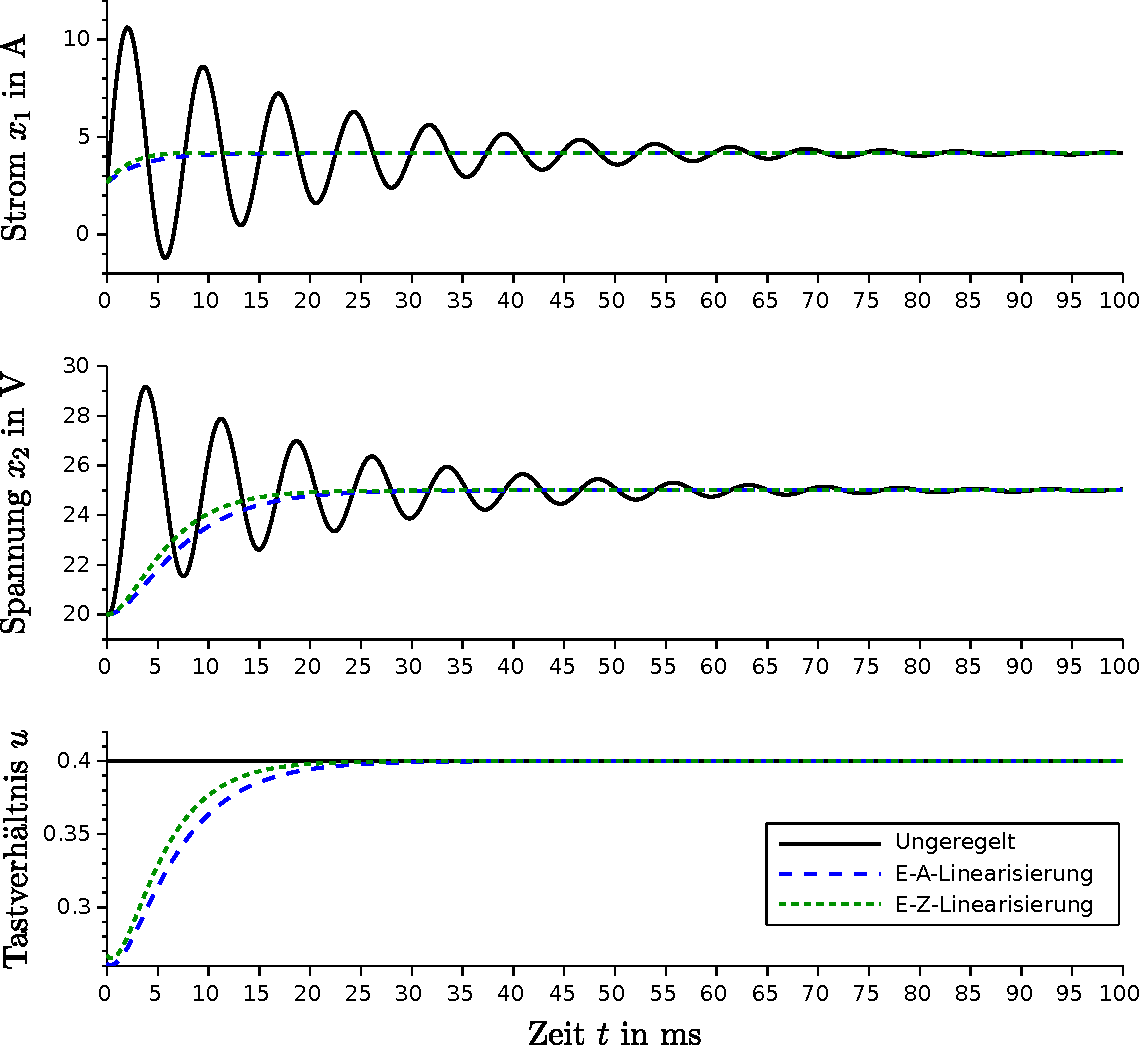
\includegraphics[width=0.9\textwidth]{Hochsetzsteller_Simulation}
\par\end{centering}
\caption{Simulation des gemittelten Hochsetzstellers\label{fig:Simulation-Hochsetzsteller}}
\end{figure}

\bibliographystyle{babalpha}
\bibliography{dynamic}




\chapter{Erweiterte Regelungskonzepte auf Basis der exakten Linearisierung\label{chap:regler-varianten}}

Aufbauend auf den in Kapitel~\ref{chap:regler-grundlagen} entwickelten
Konzepten (relativer Grad und bestimmte Normalformen) lassen sich
etliche verschiedene Regler realisieren und damit auch unterschiedliche
regelungstechnische Aufgabenstellungen lösen~\cite{henson1997chap4}.
In diesem Kapitel werden verschiedene Regelungskonzepte, die auf der
exakten Linearisierung aufbauen, vorgestellt. Den nachfolgenden Betrachtungen
wird ein eingangsaffines Modell für die Regelstrecke zugrunde gelegt.
Während für theoretische Untersuchungen die Byrnes-Isidori-Normalform
bevorzugt wird, erfolgen praktische Berechnung oft mit der Eingangs-Ausgangs-Normalform.
Daher sind die vorgestellten Entwurfsverfahren auch leicht auf nicht
eingangsaffine Systeme zu übertragen.

\section{Trajektorienfolgeregelung mittels Rückführung (Feed\-back)\label{sec:Trajektorienfolgeregelung-Feedback}}

\subsection{Ausgangsfolgeregelung\label{subsec:Ausgangsfolgeregelung}}

Man betrachte eine eingangsaffine Regelstrecke der Form
\begin{equation}
\dot{x}=f(x)+g(x)u,\quad y=h(x)\label{eq:var-basissystem}
\end{equation}
mit glatten Vektorfeldern $f,g,:\mathcal{M}\to\R^{n}$ und einem glatten
Skalarfeld $h:\mathcal{M}\to\R$, wobei die Felder auf einer offenen
Menge $\mathcal{M}\subseteq\R^{n}$ definiert sind. Auf Basis der
Eingangs-Ausgangs-Linearisierung wird nachfolgend eine Ausgangsfolgeregelung
entworfen. Der Systemausgang~$y$ soll sich dabei asymp\-totisch
einem Referenzverlauf $y_{\text{ref}}:[0,\infty)\to\R$ annähern.
Die Darstellung beruht auf~\cite[Abschn.~{4.5}]{isidori3}.

System~(\ref{eq:var-basissystem}) habe einen wohldefinierten relativen
Grad $r\leq n$. Dann kann das System mit einer Zustandstransformation
$(\xi,\eta)=\Phi(x)$ in die Byrnes-Isidori-Normalform\index{Normalform!Byrnes-Isidori-}
\begin{equation}
\left.\begin{array}{lcl}
\dot{\xi}_{1} & = & \xi_{2}\\
 & \vdots\\
\dot{\xi}_{r-1} & = & \xi_{r}\\
\dot{\xi}_{r} & = & \alpha(\xi,\eta)+\beta(\xi,\eta)u\\
\dot{\eta}_{1} & = & q_{1}(\xi,\eta)\\
 & \vdots\\
\dot{\eta}_{n-r} & = & q_{n-r}(\xi,\eta)\\
y & = & \xi_{1}
\end{array}\right\} \quad\begin{array}{rcl}
\dot{\xi} & = & A\xi+b(\alpha(\xi,\eta)+\beta(\xi,\eta)u)\\
\dot{\eta} & = & q(\xi,\eta)\\
y & = & c^{T}\xi
\end{array}\label{eq:var-BI-NF}
\end{equation}
transformiert werden (siehe Abschnitt~\ref{subsec:Byrnes-Isidori-Normalform}).
Mit der Eingangs-Ausgangs-Linearisierung 
\begin{equation}
u=\frac{1}{\beta(\xi,\eta)}\left(v-\alpha(\xi,\eta)\right)=\frac{1}{L_{g}L_{f}^{r-1}h(x)}\left(v-L_{f}^{r}h(x)\right)\label{eq:var-linearisierung-FB}
\end{equation}
kompensiert man die im ersten Teilsystem von~(\ref{eq:var-BI-NF})
auftretenden Nichtlinearitäten derart, dass das Eingangs-Ausgangs-Verhalten
durch die Integratorkette
\begin{equation}
\left.\begin{array}{lcl}
\dot{\xi}_{1} & = & \xi_{2}\\
 & \vdots\\
\dot{\xi}_{r-1} & = & \xi_{r}\\
\dot{\xi}_{r} & = & v\\
y & = & \xi_{1}
\end{array}\right\} \quad\begin{array}{rcl}
\dot{\xi} & = & A\xi+bv\\
y & = & c^{T}\xi
\end{array}\label{eq:var-TS1-EA-linearisiert}
\end{equation}
beschrieben wird.

Zur Beschreibung des Folgeverhaltens wird der Fehler 
\begin{equation}
\varepsilon(t):=y(t)-y_{\text{ref}}(t)\quad\text{für}\quad t\geq0\label{eq:var-ausgangsfehler}
\end{equation}
als Differenz zwischen System- und Referenzausgang eingeführt. Für
den Zeitverlauf des Fehlers~$\varepsilon$ geben wir eine Fehlerdynamik
in Form einer linearen zeitinvarianten Differentialgleichung 
\begin{equation}
\varepsilon^{(r)}(t)+a_{r-1}\varepsilon^{(r-1)}(t)+\cdots+a_{1}\dot{\varepsilon}(t)+a_{0}\varepsilon(t)=0\label{eq:var-fehlerdynamik}
\end{equation}
der Ordnung~$r$ vor. Die Koeffizienten $a_{0},\ldots a_{r-1}\in\R$
sind dabei so zu wählen, dass das zu~(\ref{eq:var-fehlerdynamik})
gehörende charakteristische Polynom ein Hurwitz-Polynom ist. Dann
gilt 
\[
\lim_{t\to\infty}\varepsilon(t)\to0
\]
für alle Anfangswerte von~(\ref{eq:var-fehlerdynamik}), wodurch
das asymptotische Folgeverhalten gewährleistet ist.

Die gewünschte Fehlerdynmik~(\ref{eq:var-fehlerdynamik}) ist jetzt
noch in das System einzuprägen. Der vorgegebene Referenzverlauf $y_{\text{ref}}:[0,\infty)\to\R$
des Ausgangs sei $r$ mal stetig differenzierbar. Aus~(\ref{eq:var-ausgangsfehler})
folgt unmittelbar $\varepsilon^{(i)}(t)=y^{(i)}(t)-y_{\text{ref}}^{(i)}(t)$
für $i=0,\ldots,r$. Für die Integratorkette~(\ref{eq:var-TS1-EA-linearisiert})
ergibt sich daraus der Eingangsverlauf
\begin{equation}
\begin{array}{lcl}
v(t) & = & y^{(r)}(t)\\
 & = & y_{\text{ref}}^{(r)}(t)+\varepsilon^{(r)}(t)\\
 & = & y_{\text{ref}}^{(r)}(t)-a_{r-1}\varepsilon^{(r-1)}(t)-\cdots-a_{1}\dot{\varepsilon}(t)-a_{0}\varepsilon(t).
\end{array}\label{eq:var-PD-verallg}
\end{equation}
Ersetzt man die Zeitableitungen des Systemausgangs durch Lie-Ableitungen
$y^{(i)}(t)=L_{f}^{i}h(x(t))$ für $i=1,\ldots,r-1$ und bezieht die
linearisierende Zustandsrückführung~(\ref{eq:var-linearisierung-FB})
ein, so erhält man das Regelgesetz 
\begin{equation}
u=\frac{1}{L_{g}L_{f}^{r-1}h(x)}\left(y_{\text{ref}}^{(r)}(t)-L_{f}^{r}h(x)+\sum_{i=0}^{r-1}a_{i}\left(y_{\text{ref}}^{(i)}(t)-L_{f}^{i}h(x)\right)\right).\label{eq:folgeregelung-feedback}
\end{equation}
Dieses Regelgesetz kann man als Linearkombination 
\[
u=u_{\text{steuer}}+u_{\text{stab}}
\]
eines Anteils zur Vorsteuerung
\begin{equation}
u_{\text{steuer}}=\frac{1}{L_{g}L_{f}^{r-1}h(x)}\left(y_{\text{ref}}^{(r)}(t)-L_{f}^{r}h(x)\right)\label{eq:u-steuer-FB}
\end{equation}
und eines Anteils zur asymptotischen Stabilisierung 
\begin{equation}
u_{\text{stab}}=\frac{1}{L_{g}L_{f}^{r-1}h(x)}\sum_{i=0}^{r-1}a_{i}\left(y_{\text{ref}}^{(i)}(t)-L_{f}^{i}h(x)\right)\label{eq:u-stab-FB}
\end{equation}
auffassen. Man spricht dabei von einer \emph{Struktur mit zwei Freiheits\-graden}~\cite{horowitz1963synthesis,kreisselmeier1999}.
Der Steuerungsanteil~(\ref{eq:u-steuer-FB}) wird unter Verwendung
der Hirschorn-Inversen\index{Hirschorn-Inverse} entlang der Systemtrajektorie~$x$
gebildet (siehe Anmerkung~\ref{rem:Hirschorn-Inverse}). Ein Trajektoriengenerator
stellt die Referenztrajektorie bereit. Abb.~\ref{fig:Trajektorienfolgeregelung-FB}
verdeutlicht das Zusammenwirken der verschiedenen Anteile im geschlossenen
Regelkreis.

\begin{figure}
\begin{centering}
\resizebox{0.95\textwidth}{!}{\input{Traj_FB.pdftex_t}}
\par\end{centering}
\caption{Struktur der Trajektorienfolgeregelung mittels Rückführung\label{fig:Trajektorienfolgeregelung-FB}}

\end{figure}

\medskip{}

Durch die im Regelgesetz~(\ref{eq:folgeregelung-feedback}) auftretende
Referenztrajektorie $t\mapsto y_{\text{ref}}(t)$ ist das rückgeführte
System zeitvariant, so dass man die Stabilitätsaussagen aus den Sätzen~\ref{thm:Stabilisierung-EA-lokal}
oder~\ref{thm:Stabilisierung-EA-global} nicht unmittelbar übernehmen
kann. Allerdings lassen sich die Überlegungen von Satz~\ref{thm:Stabilisierung-EA-global-fuehrungssignal}
übertragen. Dazu betrachten wir das System~(\ref{eq:var-basissystem})
in der Byrnes-Isidori-Normalform~(\ref{eq:var-BI-NF}). Der Zustand~$\xi$
des ersten Teilsystems von~(\ref{eq:var-BI-NF}) ist durch den Ausgang
und seine Zeitableitungen gegeben:
\begin{equation}
\xi_{1}=y,\,\xi_{2}=\dot{y},\,\ldots,\,\xi_{r}=y^{(r-1)}.\label{eq:Zustand-xi-durch-y}
\end{equation}
Der Referenzzustand $\xi_{\text{ref}}$ lässt sich in gleicher Weise
durch $\xi_{1,\text{ref}}=y_{\text{ref}},\ldots,\xi_{r,\text{ref}}=y_{\text{ref}}^{(r-1)}$
beschreiben. Die Differenz $\tilde{\xi}=\xi-\xi_{\text{ref}}$ liefert
die Koordinaten des Fehlersystems mit $\tilde{\xi}_{1}=\varepsilon,\ldots,\tilde{\xi}_{r}=\varepsilon^{(r-1)}$.
Die Fehlerdynamik~(\ref{eq:var-fehlerdynamik}) lässt sich dann als
Zustandsraummodell
\begin{equation}
\left.\begin{array}{lcl}
\dot{\tilde{\xi}}_{1} & = & \tilde{\xi}_{2}\\
 & \vdots\\
\dot{\tilde{\xi}}_{r-1} & = & \tilde{\xi}_{r}\\
\dot{\tilde{\xi}}_{r} & = & -a_{0}\tilde{\xi}_{1}-\cdots-a_{r-1}\tilde{\xi}_{r}
\end{array}\right\} \quad\dot{\tilde{\xi}}=(A-bk^{T})\,\tilde{\xi}\label{eq:folgesystem-FB1}
\end{equation}
mit $k=(a_{0},\ldots,a_{r-1})^{T}$ angeben. Mit $\xi=\xi_{\text{ref}}+\tilde{\xi}$
ergibt sich für das zweite Teilsystem die Form
\begin{equation}
\dot{\eta}=q(\xi_{\text{ref}}+\tilde{\xi},\eta).\label{eq:folgesystem-FB2}
\end{equation}

Nach diesen Vorüberlegungen kann folgende Aussage getroffen werden:
\begin{theorem}
\label{thm:Stabilisierung-FB}Das System~(\ref{eq:var-basissystem})
habe den Arbeitspunkt $p\in\mathcal{M}$ (für $u=0$) und den gleichmäßigen
relativen Grad $r<n$. Zusätzlich sei das System global rück\-führ\-äquivalent
zu der Form~(\ref{eq:var-BI-NF}) mit der Ruhelage $(\xi,\eta)=(0,0)$.
Die Reglerverstärkung $k\in\R^{r}$ sei so gewählt, dass das zur Fehlerdynamik~(\ref{eq:var-fehlerdynamik})
gehörende charakteristische Polynom ein Hurwitz-Polynom ist. Zusätzlich
sei der Referenzverlauf~$y_{\text{ref}}$ bis zur Ableitungsordnung
$r-1$ beschränkt, d.\,h. es gibt eine Schranke $M>0$, so dass
\begin{equation}
\left|y_{\text{ref}}^{(i)}(t)\right|<M\label{eq:yref-beschraenkt-in-Cr}
\end{equation}
für alle $t\geq0$ und $i=0,\ldots,r-1$. Ist das System stark minimalphasig,
dann bleiben die Systemtrajektorien beschränkt.
\end{theorem}
\begin{svmultproof2}
Da globale Rückführäquivalenz zur Form~(\ref{eq:var-BI-NF}) angenommen
wird, kann die Stabilitätsbetrachtung auf Basis der Gln.~(\ref{eq:folgesystem-FB1})
und~(\ref{eq:folgesystem-FB2}) erfolgen. Weil alle Eigenwerte der
Matrix $A-bk^{^{T}}$nach Wahl der Reglerverstärkung~$k$ negative
Realteile besitzen, klingt~$\tilde{\xi}$ ab, d.\,h. $\tilde{\xi}(t)\to0$
für $t\to\infty$. Damit ist~$\tilde{\xi}$ beschränkt. Mit Gl.~(\ref{eq:yref-beschraenkt-in-Cr})
ist~$\xi_{\text{ref}}$ und damit die auch Summe $\xi_{\text{ref}}+\tilde{\xi}$
beschränkt. Mit der angenommenen starken Minimalphasigkeit ist das
zweite Teilsystem~(\ref{eq:folgesystem-FB2}) eingangs-zustands-stabil,
so dass $\eta$ beschränkt bleibt. Da die Transformation ein globaler
Diffeomorphismus ist, bleibt auch die System\-trajektorie~$x$ beschränkt.
\end{svmultproof2}

Für $r=n$ tritt das zweites Teilsystem~(\ref{eq:folgesystem-FB2})
nicht auf. In diesem Fall erhält man durch~(\ref{eq:folgesystem-FB1})
insgesamt eine lineare zeitinvariante Fehlerdynamik.

\medskip{}

Die dargelegten Überlegungen lassen sich unmittelbar auf Mehr\-größen\-systeme
übertragen. Die Kompensation der Nichtlinearitäten erfolgt simultan
mit der Entkopplung der Teilsysteme (siehe Abschnitt~\ref{sec:Mehrvariable-Systeme}).
Die Trajektorienfolgeregelung wird dann für jeden einzelnen Ausgang
in der beschriebenen Weise durchgeführt. Bei einem vollständig aktuierten
mechanischen System lässt sich die Trajektorienfolgeregelung besonders
einfach gestalten: 
\begin{remark}
\label{rem:Mechanisches-System-Feedback}Wir betrachten ein mechanisches
System, welches durch eine Bewegungsgleichung der Form 
\begin{equation}
M(q)\ddot{q}+C(q,\dot{q})=\tau\label{eq:mani-euler-lagrange-tracking}
\end{equation}
mit den verallgemeinerten Positionen~$q$, den verallgemeinerten
Geschwindigkeiten~$\dot{q}$ und der Massenmatrix $M(q)$ beschrieben
wird. Der Vektor~$\tau$ enthält die eingeprägten Kräfte bzw. Momente
und der Vektor $C(q,\dot{q})$ alle weiteren Kräfte. Die Forderung
\[
\ddot{q}\stackrel{!}{=}v
\]
einer exakten Kompensation der Nichtlinearitäten führt zunächst auf
das (linearisierende) Stellgesetz
\begin{equation}
\tau=M(q)\,v+C(q,\dot{q}),\label{eq:mech-linearisierung-feedback}
\end{equation}
vgl. Anmerkung~\ref{rem:Mechanisch-relativer-grad}. Die Stabilisierung
entlang einer zweimal stetig differenzierbaren Referenztrajektorie~$q_{\text{ref}}$
erfolgt durch die als PD-Regler\index{PD-Regler} interpretierbare
Rückführung
\begin{equation}
v=\ddot{q}_{\text{ref}}+K_{D}\left(\dot{q}_{\text{ref}}-\dot{q}\right)+K_{P}\left(q_{\text{ref}}-q\right)\label{eq:mech-stabiliserung}
\end{equation}
mit passenden Diagonalmatrizen~$K_{P}$ und~$K_{D}$. Setzt man
das daraus resultierende Stellgesetz 
\begin{equation}
\tau=M(q)\cdot\left[\ddot{q}_{\text{ref}}+K_{D}\left(\dot{q}_{\text{ref}}-\dot{q}\right)+K_{P}\left(q_{\text{ref}}-q\right)\right]+C(q,\dot{q})\label{eq:tau-mech-FB}
\end{equation}
in die Bewegungsgleichung~(\ref{eq:mani-euler-lagrange-tracking})
ein, so erhält man eine exakt lineare zeit\-invariante Fehlerdynamik
\[
0=\ddot{q}_{\text{ref}}-\ddot{q}+K_{D}\left(\dot{q}_{\text{ref}}-\dot{q}\right)+K_{P}\left(q_{\text{ref}}-q\right).
\]
Bei diesem Ansatz nutzt man die Bewegungsgleichung zur Berechnung
der einzuprägenden Momente. Man spricht daher von der \emph{Methode
der berechneten Momente} (engl. \emph{computed torque method}).
\end{remark}

\begin{remark}
\label{rem:PI-Feedback}PI- und PID-Regler sind in der industriellen
Praxis die am häufigsten eingesetzten Reglertypen~\cite{marlin2000,odwyer2009handbook}.
Mit dem I-Anteil lassen sich bleibende Regelabweichungen kompensieren
und Störungen unterdrücken~\cite{datta2000}. Die Rückführung~(\ref{eq:folgeregelung-feedback})
kann man unter Bezug auf Gl.~(\ref{eq:var-PD-verallg}) als verallgemeinerten
PD-Regler\index{PD-Regler} auffassen. Zur Ergänzung eines I-Anteils
erweitert man die Fehlerdynamik~(\ref{eq:var-fehlerdynamik}) zu
\[
\varepsilon^{(r)}(t)+a_{r-1}\varepsilon^{(r-1)}(t)+\cdots+a_{1}\dot{\varepsilon}(t)+a_{0}\varepsilon(t)+a_{I}\int_{0}^{t}\varepsilon(\tau)\d\tau=0
\]
mit dem zusätzlichen Koeffizienten $a_{I}>0$. Der I-Anteil wird dabei
nach der Kompensation der Nichtlinearitäten durch~(\ref{eq:var-linearisierung-FB})
eingefügt. In den Originalkoordinaten erhält man daraus die Zustandsrückführung
\[
u=\frac{1}{L_{g}L_{f}^{r-1}h(x)}\left(a_{I}\!\int_{0}^{t}\!\left(y_{\text{ref}}(\tau)-h(x(\tau))\right)\d\tau+\sum_{i=0}^{r}a_{i}\left(y_{\text{ref}}^{(i)}(t)-L_{f}^{i}h(x)\right)\right)
\]
mit $a_{r}:=1$, vgl.~\cite{kravaris1987,henson1991critique}. Diese
Rückführung lässt sich als verallgemeinerter PID-Regler\index{PID-Regler}
interpretieren~\cite{sira-ramirez2002gpid}. Alternativ kann man
dem (nicht eingangs-ausgangs-linearisierten) Originalsystem auch einen
Integrator vorschalten~\cite{mahout2003}. Das erweiterte System
hat dann den relativen Grad $r+1$ (vgl. Abschnitt~\ref{subsec:Relativer-Grad-nichtaffine})
und kann mit der hinsichtlich~$r$ entsprechend an\-ge\-passten
Rückführung~(\ref{eq:folgeregelung-feedback}) geregelt werden.
\end{remark}

\subsection{Überführung zwischen Ruhelagen\label{subsec:Ueberfuehrung-zwischen-Ruhelagen}}

Eine besonders praxisrelevante Aufgabenstellung im Rahmen der Trajektorienfolgeregelung
ist die Überführung des Systems von einer Ruhelage $x^{0}\in\mathcal{M}$
in eine andere Ruhelage $x^{1}\in\mathcal{M}$. Hinsichtlich des Ausgangs
bedeutet das einen Übergang von $y^{0}=h(x^{0})$ zu $y^{1}=h(x^{1})$.
Gesucht ist ein Referenzverlauf $y_{\text{ref}}:[0,T]\to\R$ des Ausgangs,
so dass die Ruhelage $x^{0}=x(0)$ in die Ruhelage $x^{1}=x(T)$ überführt
wird (siehe Abb.~\ref{fig:Referenztrajektorie-Ausgang}). Die Ruhelagenüberführung
erfolgt in diesem Abschnitt für das durch Rückführung linearisierte
erste Teil\-system~(\ref{eq:var-TS1-EA-linearisiert}). Die Überführung
des Zustands~$x$ bzw. $(\xi,\eta)$ des Gesamtsystems wird in Abschnitt~\ref{sec:Trajektorienfolgeregelung-Feedforward}
behandelt. 
\begin{figure}
\begin{centering}
\resizebox{0.7\textwidth}{!}{\input{Ruhelagenueberfuehrung.pdftex_t}}
\par\end{centering}
\caption{Referenztrajektorie des Ausgangs bei einer Ruhelagenüberführung\label{fig:Referenztrajektorie-Ausgang}}
\end{figure}

Der Zustand~$\xi$ des Systems~(\ref{eq:var-TS1-EA-linearisiert})
lässt sich durch den Ausgang und seine Zeitableitungen erfassen, vgl.
Gl.~(\ref{eq:Zustand-xi-durch-y}). Die Ruhelagen vor und nach dem
Überführungsvorgang sind daher durch die $2r$ Randbedingungen
\begin{equation}
\begin{array}{llll}
y_{\text{ref}}(0)=y^{0}, & \dot{y}_{\text{ref}}(0)=0, & \ldots, & y_{\text{ref}}^{(r-1)}(0)=0\\
y_{\text{ref}}(T)=y^{1}, & \dot{y}_{\text{ref}}(T)=0, & \ldots, & y_{\text{ref}}^{(r-1)}(T)=0
\end{array}\label{eq:var-randbedingungungen1}
\end{equation}
eindeutig festgelegt. Wählt man für die Überführung zwischen den Ruhelagen
einen hinreichend glatten Verlauf des Referenzausgangs $y_{\text{ref}}:[0,T]\to\R$,
so dass diese Randbedingungen erfüllt sind, dann erhält man damit
auch einen stetigen Übergang des Zustands~$\xi$. Fordert man zusätzlich
\begin{equation}
y_{\text{ref}}^{(r)}(0)=y_{\text{ref}}^{(r)}(T)=0,\label{eq:var-randbedingungungen2}
\end{equation}
dann ist wegen der letzten Differentialgleichung von~(\ref{eq:var-TS1-EA-linearisiert})
auch der für die Überführung benötigte Eingangsverlauf stetig. Mit
den Gln.~(\ref{eq:var-randbedingungungen1}) und~(\ref{eq:var-randbedingungungen2})
ergeben sich insgesamt $2r+2$ Randbedingungen, die der gesuchte Referenzverlauf
$y_{\text{ref}}$ des Ausgangs erfüllen soll.

Für den Übergang von $y^{0}=y_{\text{ref}}(0)$ zu $y^{1}=y_{\text{ref}}(T)$
unter Beachtung der o.\,g. Randbedingungen könnte man aus einer großen
Menge möglicher Ansatzfunktionen wählen (z.\,B. Splines oder Linearkombinationen
trigonometrischer Funktionen). Ein besonders einfacher Ansatz ist
durch ein Polynom gegeben. Um nicht in jedem Einzelfall das benötigte
Polynom erneut auszurechnen bietet es sich an, ein normiertes Polynom~$\sigma$
zu bestimmen, welches von $\sigma(0)=0$ auf $\sigma(1)=1$ unter
Berücksichtigung der entsprechenden Randbedingungen in den Ableitungen
übergeht. Für $2r+2$ Parameter muss das Polynom~$\sigma$ mindestens
mit dem Grad $2r+1$ angesetzt werden.
\begin{example}
\label{exa:normiertes-uebergangspolynom}Für $r=1$ würde man ein
Polynom von Grad $2r+1=3$ ansetzen:
\[
\sigma(t)=\sigma_{0}+\sigma_{1}t+\sigma_{2}t^{2}+\sigma_{3}t^{3}.
\]
Die Parameter~$\sigma_{0}$ und~$\sigma_{1}$ erhält man aus den
Bedingungen am linken Rand:
\[
\begin{array}{lclcl}
\sigma(0) & = & \sigma_{0} & \stackrel{!}{=} & 0,\\
\dot{\sigma}(0) & = & \sigma_{1} & \stackrel{!}{=} & 0.
\end{array}
\]
Die Bedingungen am rechten Rand 
\[
\left.\begin{array}{lclcl}
\sigma(1) & = & \sigma_{2}+\sigma_{3} & \stackrel{!}{=} & 1\\
\dot{\sigma}(1) & = & 2\sigma_{2}+3\sigma_{3} & \stackrel{!}{=} & 0
\end{array}\right\} \quad\Leftrightarrow\quad\left(\begin{array}{cc}
1 & 1\\
2 & 3
\end{array}\right)\left(\begin{array}{c}
\sigma_{2}\\
\sigma_{3}
\end{array}\right)=\left(\begin{array}{c}
1\\
0
\end{array}\right)
\]
liefern $\sigma_{2}=3$ und $\sigma_{3}=-2$ und damit $\sigma(t)=3t^{2}-2t^{3}$. 

\end{example}
Der in Beispiel~\ref{exa:normiertes-uebergangspolynom} beschriebene
Ansatz führt bei polynomialen Ansatzfunktionen immer auf ein lineares
Gleichungssystem. Allerdings können die gesuchten Übergangspolynome
auch über eine direkte Formel berechnet werden~\cite{piazzi2001tac,piazzi2001automatica}:
\begin{equation}
\sigma(t)=\frac{(2r+1)!}{r!}\sum_{i=r+1}^{2r+1}\frac{(-1)^{i-r-1}}{(i-r-1)!\,(2r+1-i)!\cdot i}\,t^{i}.\label{eq:formel-uebergangspolynom}
\end{equation}
Basierend auf dem normierten Übergangspolynom~$\sigma$ lässt sich
jetzt der Übergang von $y^{0}=y_{\text{ref}}(0)$ zu $y^{1}=y_{\text{ref}}(T)$
durch die abschnittsweise definierte Funktion
\begin{equation}
y_{\text{ref}}(t)=\left\{ \begin{array}{ccl}
y^{0} &  & t<0\\
y^{0}+(y^{1}-y^{0})\cdot\sigma\left(\frac{t}{T}\right) & \quad\text{für}\quad & 0\leq t\leq T\\
y^{1} &  & t>T
\end{array}\right.\label{eq:yref-allgemein}
\end{equation}
spezifizieren (vgl. Abb.~\ref{fig:Referenztrajektorie-Ausgang}).

\begin{example}
\label{exa:hochsetzsteller-folgeregelung-feedback}Man betrachte das
gemittelte Modell des Hochsetzstellers\index{Hochsetzsteller} aus
Abschnitt~\ref{subsec:Hochsetzsteller} mit den dort angegebenen
Parameterwerten:
\begin{equation}
\begin{array}{lcl}
\dot{x}_{1} & = & -(1-u)\frac{1}{L}x_{2}+\frac{E}{L},\\
\dot{x}_{2} & = & (1-u)\frac{1}{C}x_{1}-\frac{1}{RC}x_{2}.
\end{array}\label{eq:var-hochsetzsteller}
\end{equation}
Gewünscht ist ein Übergang der Ausgangsspannung von $20\,\text{V}$
auf $25\,\text{V}$ in einem Zeitintervall der Länge $T=50\,\text{ms}$.

Verwendet man für den Reglerentwurf den Strom\footnote{Aus Anwendungssicht wäre es wünschenswert, die Spannung direkt als
Referenzgröße nutzen zu können. Mit dem hier beschriebenen Zugang
ist das leider nicht möglich, da die zugehörige Nulldynamik instabil
ist (vgl. Abschnitt~\ref{subsec:Hochsetzsteller-Ausgang-Spannung}).} als Ausgang
\begin{equation}
y=h(x)=x_{1},\label{eq:hochsetzsteller-ausgang-strom-tracking}
\end{equation}
so hat das System den relativen Grad $r=1$. Damit lässt sich das
normierte Übergangspolynom $\sigma(t)=3t^{2}-2t^{3}$ aus Beispiel~\ref{exa:normiertes-uebergangspolynom}
nutzen. Der Übergang zwischen den o.\,g. Spannungen entspricht einem
Übergang des Stroms von $y^{0}=x_{1}(0)=2,\bar{6}\,\text{\text{A}}$
auf $y^{1}=x_{1}(T)=4,1\bar{6}\,\text{A}$. Auf Basis des sich daraus
ergebenden Referenzverlaufs
\begin{equation}
y_{\text{ref}}(t)=\frac{8}{3}+1800t^{2}-24000t^{3}\label{eq:hochsetzsteller-yref-strom}
\end{equation}
nach Gl.~(\ref{eq:yref-allgemein}) mit $t$ in~$\text{s}$ und~$y_{\text{ref}}$
in~$\text{A}$ nimmt das Regelgesetz~(\ref{eq:folgeregelung-feedback})
die Form
\end{example}
\begin{eqnarray*}
u & = & \frac{1}{L_{g}h(x)}\left(\dot{y}_{\text{ref}}(t)-L_{f}h(x)+a_{0}(y_{\text{ref}}(t)-h(x))\right)\\
 & = & \frac{L}{x_{2}}\left(\dot{y}_{\text{ref}}(t)-\frac{E-x_{2}}{L}+a_{0}(y_{\text{ref}}(t)-x_{1})\right)
\end{eqnarray*}
mit einem Koeffizienten $a_{0}>0$ an.

Verwendet man alternativ die elektrische Energie als Ausgang 
\begin{equation}
y=h(x)=\frac{L}{2}x_{1}^{2}+\frac{C}{2}x_{2}^{2},\label{eq:hochsetzsteller-ausgang-energie-tracking}
\end{equation}
so hat das System den relativen Grad $r=2$, d.\,h. man führt eine
Eingangs-Zustands-Linearisierung durch. Aus Gl.~(\ref{eq:formel-uebergangspolynom})
erhält man das Übergangspolynom $\sigma(t)=10t^{3}-15t^{4}+6t^{5}$.
Für~(\ref{eq:hochsetzsteller-ausgang-energie-tracking}) wird der
Übergang von $y^{0}=0,201\bar{7}\,\text{Ws}$ auf $y^{1}=0,3168402\bar{7}\,\text{Ws}$
entsprechend Gl.~(\ref{eq:yref-allgemein}) geplant 
\begin{equation}
y_{\text{ref}}(t)=0,201\bar{7}+9205t^{3}-276150t^{4}+2209200t^{5},\label{eq:hochsetzsteller-yref-energie}
\end{equation}
wobei $t$ in~$\text{s}$ und $y_{\text{ref}}$ in~$\text{Ws}$
angegeben sind. Das Regelgesetz hat die Gestalt 
\[
u=\frac{1}{L_{g}L_{f}h(x)}\left(\ddot{y}_{\text{ref}}(t)\!-\!L_{f}^{2}h(x)+a_{1}((\dot{y}_{\text{ref}}(t)\!-\!L_{f}h(x)))+a_{0}(y_{\text{ref}}(t)\!-\!h(x))\right)
\]
mit den Lie-Ableitungen aus Gl.~(\ref{eq:Hochsetzsteller-Lie-Ableitungen-Energie})
und den Koeffizienten $a_{0},a_{1}>0$ (Stodola-Bedingung).

Abb.~\ref{fig:Hochsetzsteller-Tracking} zeigt die numerischen Ergebnisse
für beide Fälle ($r=1$ bzw. $r=2$ für Eingangs-Ausgangs- bzw. Eingangs-Zustands-Linearisierung).
Die Koeffizienten $a_{0},a_{1}$ der Reglerverstärkung wurden entsprechend
Abschnitt~\ref{subsec:Hochsetzsteller} gewählt. Mit der Eingangs-Zustands-Linearisierung
ist ein schnelleres Einschwingen möglich. Allerdings weist der Strom
in diesem Fall auch ein leichtes Überschwingen auf (Abb.~\ref{fig:Hochsetzsteller-Tracking}
oben).

\begin{figure}
\begin{centering}
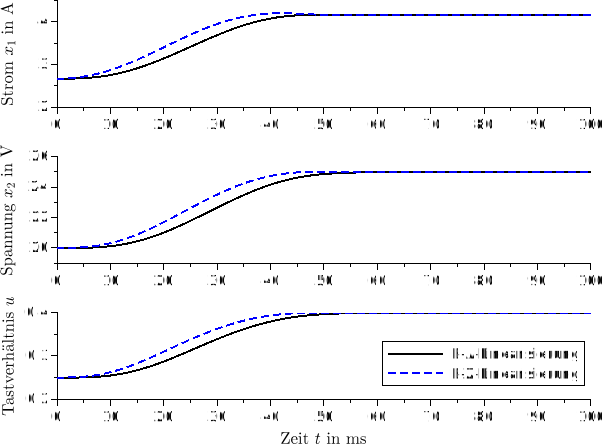
\includegraphics[width=0.8\textwidth]{Hochsetzsteller_Tracking_FB}
\par\end{centering}
\caption{Referenztrajektorien bzw. Simulation des ungestörten Hochsetzstellers\label{fig:Hochsetzsteller-Tracking}}
\end{figure}


\section{Trajektorienfolgeregelung mittels Aufschaltung (Feed\-forward)\label{sec:Trajektorienfolgeregelung-Feedforward}}

\subsection{Folgeregelung entlang einer bekannten Referenztrajektorie}

Wir widmen uns weiterhin dem Problem der Trajektorienfolgeregelung
und betrachten die in~\cite{hagenmeyer2003lncis,hagenmeyer2003}\nocite{zinober2003}
vorgestellten Lösungsansätze. Dabei gehen wir jetzt von einem bekannten
Referenzverlauf $x_{\text{ref}}:[0,T]\to\mathcal{M}$ des Zustands
aus. Befindet sich der Zustand des Systems~(\ref{eq:var-basissystem})
bereits auf der Referenztrajektorie, d.\,h. $x=x_{\text{ref}}$,
dann kann die in Gl.~(\ref{eq:var-linearisierung-FB}) durchgeführte
Kompensation der Nichtlinearitäten des ersten Teilsystems von~(\ref{eq:var-BI-NF})
auch auf Basis des Referenzzustands mit $(\xi_{\text{ref}},\eta_{\text{ref}})=\Phi(x_{\text{ref}})$
erfolgen: 
\begin{equation}
u=\frac{1}{\beta(\xi_{\text{ref}},\eta_{\text{ref}})}\left(v-\alpha(\xi_{\text{ref}},\eta_{\text{ref}})\right)=\frac{1}{L_{g}L_{f}^{r-1}h(x_{\text{ref}})}\left(v-L_{f}^{r}h(x_{\text{ref}})\right).\label{eq:var-linearisierung-FF}
\end{equation}
Zusammen mit der aus der vorgegebenen Fehlerdynamik~(\ref{eq:var-fehlerdynamik})
hergeleiteten Rückführung~(\ref{eq:folgeregelung-feedback}) erhält
man insgesamt das Regelgesetz 
\begin{equation}
u=\frac{1}{L_{g}L_{f}^{r-1}h(x_{\text{ref}}(t))}\left(y_{\text{ref}}^{(r)}(t)-L_{f}^{r}h(x_{\text{ref}}(t))+\sum_{i=0}^{r-1}a_{i}\left(y_{\text{ref}}^{(i)}(t)-L_{f}^{i}h(x)\right)\right).\label{eq:folgeregelung-feedforward}
\end{equation}
Der Unterschied zu dem Regelgesetz~(\ref{eq:folgeregelung-feedback})
besteht lediglich darin, dass die höchsten Lie-Ableitungen $L_{f}^{r}h(x)$
und $L_{g}L_{f}^{r-1}h(x)$ entlang der Referenztrajektorie~$x_{\text{ref}}$
anstelle der Systemtrajektorie~$x$ ausgewertet werden. Bei diesem
Zugang erwartet man im Vergleich zur Trajektorienfolgeregelung~(\ref{eq:folgeregelung-feedback})
mittels Rückführung eine größere Robustheit gegenüber Modellunbestimmtheiten.

Auch bei Gl.~(\ref{eq:folgeregelung-feedforward}) ist eine Aufspaltung
\begin{equation}
u=u_{\text{ref}}+u_{\text{stab}}\label{eq:u-aufspaltung-FF}
\end{equation}
in einen Anteil der Vorsteuerung
\begin{equation}
u_{\text{ref}}=\frac{1}{L_{g}L_{f}^{r-1}h(x_{\text{ref}}(t))}\left(y_{\text{ref}}^{(r)}(t)-L_{f}^{r}h(x_{\text{ref}}(t))\right)\label{eq:u-steuer-FF}
\end{equation}
und einen Anteil zur asymptotischen Stabilisierung
\begin{equation}
u_{\text{stab}}=\frac{1}{L_{g}L_{f}^{r-1}h(x_{\text{ref}}(t))}\sum_{i=0}^{r-1}a_{i}\left(y_{\text{ref}}^{(i)}(t)-L_{f}^{i}h(x)\right)\label{eq:u-stab-FF}
\end{equation}
möglich. Die Steuerung~(\ref{eq:u-steuer-FF}) wird als Hirschorn-Inverse\index{Hirschorn-Inverse}
der Systemdynamik entlang der Referenztrajektorie~$x_{\text{ref}}$
gebildet und stellt damit (unabhängig vom Systemzustand~$x$) den
Referenzverlauf des Eingangssignals dar. Damit liegt hier ein inversionsbasierter
Vorsteuerungsentwurf vor~\cite{graichen2006at}. Die sich daraus
ergebende Regelkreisstruktur ist in Abb.~\ref{fig:Trajektorienfolgeregelung-FF}
dargestellt.

\begin{figure}
\begin{centering}
\resizebox{0.95\textwidth}{!}{\input{Traj_FF.pdftex_t}}
\par\end{centering}
\caption{Struktur der Trajektorienfolgeregelung mittels Aufschaltung\label{fig:Trajektorienfolgeregelung-FF}}
\end{figure}

Die beschriebene Herangehensweise lässt sich analog zur Trajektorienfolgeregelung
mittels Rückführung auch auf Mehrgrößensysteme übertragen. Der Spezialfall
vollständig aktuierter mechanischer Systemer wird in der folgenden
Anmerkung behandelt.
\begin{remark}
\label{rem:Mechanisches-System-Feedforward}Wir betrachten die Bewegungsgleichungen~(\ref{eq:mani-euler-lagrange-tracking})
aus Anmerkung~\ref{rem:Mechanisches-System-Feedback}. Die in Gl.~(\ref{eq:mech-linearisierung-feedback})
vorgenommene Kompensation der Nichtlinearitäten erfolgt jetzt allerdings
entlang der Referenztrajektorien:
\begin{equation}
\tau=M(q_{\text{ref}})\,v+C(q_{\text{ref}},\dot{q}_{\text{ref}}).\label{eq:mech-linearisierung-feedforward}
\end{equation}
Zusammen mit der Stabilisierung~(\ref{eq:mech-stabiliserung}) erhält
man das Stellgesetz
\begin{equation}
\begin{array}{lcl}
\tau & = & M(q_{\text{ref}})\cdot\left[\ddot{q}_{\text{ref}}+K_{D}\left(\dot{q}_{\text{ref}}-\dot{q}\right)+K_{P}\left(q_{\text{ref}}-q\right)\right]+C(q_{\text{ref}},\dot{q}_{\text{ref}})\\
 & = & \underbrace{M(q_{\text{ref}})\,\ddot{q}_{\text{ref}}+C(q_{\text{ref}},\dot{q}_{\text{ref}})}_{{\displaystyle \tau_{\text{ref}}}}+M(q_{\text{ref}})\left[K_{D}\left(\dot{q}_{\text{ref}}-\dot{q}\right)+K_{P}\left(q_{\text{ref}}-q\right)\right],
\end{array}\label{eq:tau-mech-FF}
\end{equation}
bei dem das aus der Bewegungsgleichung erzeugte Referenzmoment~$\tau_{\text{ref}}$
zur Vorsteuerung entsprechend Gl.~(\ref{eq:u-aufspaltung-FF}) verwendet
wird. Für $q\equiv q_{\text{ref}}$ stimmen die Rückführungen~(\ref{eq:tau-mech-FB})
und~(\ref{eq:tau-mech-FF}) überein. Bei den in~\cite{an1989} durchgeführten
Experimenten zeigen beide Regler ein ähnliches Verhalten.
\end{remark}

\begin{remark}
Die Kompensation der Nichtlinearitäten durch Aufschaltung entsprechend
Gl.~(\ref{eq:var-linearisierung-FF}) ist nur für $x=x_{\text{ref}}$
exakt. In der Regel muss man von $x\neq x_{\text{ref}}$ ausgehen,
d.\,h. der Systemzustand~$x$ wird praktisch nie exakt mit dem Referenzzustand~$x_{\text{ref}}$
übereinstimmen. Zur Kompensation der sich daraus ergebenden Regelabweichung
bietet sich die Aufschaltung eines I-Anteils an~\cite{hagenmeyer2003lncis,hagenmeyer2003}.
Dabei geht das Regelgesetz Gl.~(\ref{eq:folgeregelung-feedforward})
in den verallgemeinerten PID-Regler\index{PID-Regler}
\begin{eqnarray*}
u & = & \frac{1}{L_{g}L_{f}^{r-1}h(x_{\text{ref}}(t))}\left(y_{\text{ref}}^{(r)}(t)-L_{f}^{r}h(x_{\text{ref}}(t))\right.\\
 &  & +\left.\sum_{i=0}^{r-1}a_{i}\left(y_{\text{ref}}^{(i)}(t)-L_{f}^{i}h(x)\right)+a_{I}\!\int_{0}^{t}\!\left(y_{\text{ref}}(\tau)-h(x(\tau))\right)\d\tau\right)
\end{eqnarray*}
über (vgl. Anmerkung~\ref{rem:PI-Feedback}).
\end{remark}

\subsection{Berechnung der Referenztrajektorie bei vollem relativen Grad\label{subsec:Berechnung-Referenztraj-flach}}

Hat das System~(\ref{eq:var-basissystem}) den relativen Grad $r=n$,
dann existiert eine Zustands\-transformation $\xi=\Phi(x)$, mit
der das System in die nichtlineare Regelungsnormalform\index{Regelungsnormalform}\index{Normalform!Regelungs-}
\begin{equation}
\left.\begin{array}{lcl}
\dot{\xi}_{1} & = & \xi_{2}\\
 & \vdots\\
\dot{\xi}_{n-1} & = & \xi_{n}\\
\dot{\xi}_{n} & = & \alpha(\xi)+\beta(\xi)u\\
y & = & \xi_{1}
\end{array}\right\} \quad\begin{array}{rcl}
\dot{\xi} & = & A\xi+b(\alpha(\xi)+\beta(\xi)u)\\
y & = & c^{T}\xi
\end{array}\label{eq:var-Regelungs-NF}
\end{equation}
überführt wird. Bezogen auf Gl.~(\ref{eq:var-BI-NF}) entspricht
das dem Wegfall des zweiten Teilsystems. Wir gehen von einer bekannten
Referenztrajektorie $y_{\text{ref}}:[0,T]\to\R$ aus (siehe Abschnitt~\ref{subsec:Ueberfuehrung-zwischen-Ruhelagen}).
Nach Gl.~(\ref{eq:Zustand-xi-durch-y}) lässt sich damit der Referenzzustand
des transformierten System~(\ref{eq:var-Regelungs-NF}) berechnen.
Über die Rücktransformation $x_{\text{ref}}=\Phi^{-1}(\xi_{\text{ref}})$
erhält man die Referenztrajektorie $x_{\text{ref}}:[0,T]\to\mathcal{M}$
des Originalzustands~$x$ von System~(\ref{eq:var-basissystem}).
Aus der letzten Differentialgleichung 
\[
y^{(n)}=\dot{\xi}_{n}=\alpha(\xi)+\beta(\xi)u
\]
der Normalform~(\ref{eq:var-Regelungs-NF}) ergibt sich zusätzlich
der Referenzverlauf
\begin{equation}
\begin{array}{lcl}
u_{\text{ref}}(t) & = & \frac{1}{\beta(\xi_{\text{ref}}(t))}\left(y_{\text{ref}}^{(n)}(t)-\alpha(\xi_{\text{ref}}(t))\right)\\
 & = & \frac{1}{L_{g}L_{f}^{n-1}h(x_{\text{ref}}(t))}\left(y_{\text{ref}}^{(n)}(t)-L_{f}^{n}h(x_{\text{ref}}(t))\right)
\end{array}\label{eq:uref-feedforward-n}
\end{equation}
des Eingangs als Spezialfall von Gl.~(\ref{eq:u-steuer-FF}) für
$r=n$. Bei vollem relativen Grad ist der Ausgang~$y$ auch ein flacher
Ausgang, der zusammen mit seinen Zeitableitungen die Parametrierung
aller anderen System\-größen ermöglicht (siehe Abschnitt~\ref{sec:Flache-Systeme}). 

\begin{example}
\label{exa:hochsetzsteller-folgeregelung-feedforward-flach}Wir betrachten
das Modell~(\ref{eq:var-hochsetzsteller}) des Hochsetzstellers\index{Hochsetzsteller}
aus Beispiel~\ref{exa:hochsetzsteller-folgeregelung-feedback}. Mit
dem Ausgang~(\ref{eq:hochsetzsteller-ausgang-energie-tracking})
hat das System den vollen relativen Grad $r=2$. Die Zustände der
Regelungsnormalform~(\ref{eq:var-Regelungs-NF}) ergeben sich aus
\[
\begin{array}{lclcl}
\xi_{1} & = & h(x) & = & \frac{L}{2}x_{1}^{2}+\frac{C}{2}x_{2}^{2},\\
\xi_{2} & = & L_{f}h(x) & = & Ex_{1}-\frac{1}{R}x_{2}^{2}.
\end{array}
\]
Dieses nichtlineare Gleichungssystem lässt sich nach~$x$ auflösen
\begin{eqnarray*}
x_{1} & = & \frac{\sqrt{C^{2}E^{2}R^{2}+4CLR\xi_{2}+8\,L\xi_{1}}-CER}{2L},\\
x_{2} & = & \sqrt{R\left(Ex_{1}-\xi_{2}\right)},
\end{eqnarray*}
siehe~\cite{gensior2006} und Beispiel~\ref{exa:Hochsetzsteller-flach}
aus Abschnitt~\ref{sec:Flache-Systeme}. Durch Einsetzen der Referenzverläufe
$\xi_{1}=y_{\text{ref}}$ und $\xi_{2}=\dot{y}_{\text{ref}}$ erhält
man den Referenzzustand~$x_{\text{ref}}$. Den Referenzeingang kann
man mit Gl.~(\ref{eq:uref-feedforward-n}) in Originalkoordinaten
berechnen:
\[
u_{\text{ref}}(t)=\frac{-2Lx_{2,\text{ref}}^{2}\,+2LRx_{1,\text{ref}}x_{2,\text{ref}}+CR^{2}\left(L\ddot{y}_{\text{ref}}(t)-E^{2}+Ex_{2,\text{ref}}\right)}{R\left(CER+2Lx_{1,\text{ref}}\right)x_{2,\text{ref}}}.
\]
Mit den Parameterwerten aus Beispiel~\ref{exa:hochsetzsteller-folgeregelung-feedback}
erhält man bei vorgegebenem Referenzverlauf~(\ref{eq:hochsetzsteller-yref-energie})
die bereits in Abb.~\ref{fig:Hochsetzsteller-Tracking} für die Eingangs-Zustands-Linearisierung
angegebenen Verläufe.
\end{example}

\begin{remark}
Die symbolische Berechnung der benötigten Refernzverläufe ist bei
eingangs-zustands-linearisierbaren bzw. flachen Systemen immer möglich,
aber mitunter aufwendig. Eine numerische Methode zur punktweisen Berechnung
der Eingangs- und Zustandsreferenzverläufe bei gegebener Ausgangsreferenztrajektorie
mit Hilfe des algorithmischen Differenzieren wird in~\cite{roebvogel2000,roebenack2004automatica,roebenack2005habil}
beschrieben.
\end{remark}

\subsection{Berechnung der Referenztrajektorie bei nicht vollem relativen Grad\label{subsec:Berechnung-Referenztraj-randwert}}

Dieser Abschnitt befasst sich mit der Berechnung einer Referenztrajektorie
auf Basis des in~\cite{graichen2005,graichen2005ecc,graichen2006at}
vorgeschlagenen Verfahrens, mit der das System~(\ref{eq:var-basissystem})
von einer Ruhelage $x^{0}\in\mathcal{M}$ in eine zweite Ruhelage
$x^{1}\in\mathcal{M}$ überführt wird. Nachdem der Fall $r=n$ in
Abschnitt~\ref{subsec:Berechnung-Referenztraj-flach} behandelt wurde
gehen wir jetzt von einem relativen Grad $r<n$ aus. Damit existiert
zwar die Byrnes-Isidori-Normalform~(\ref{eq:var-BI-NF}), diese ist
allerdings oft schwer zu berechnen (vgl. Anmerkung~\ref{rem:Berechnung-Byrnes-Isidori-NF}).
Daher betrachten wir jetzt die leichter aufzustellende Eingangs-Ausgangs-Normalform\index{Normalform!Eingangs-Ausgangs-}
\begin{equation}
\begin{array}{rcl}
\dot{\xi} & = & A\xi+b(\alpha(\xi,\eta)+\beta(\xi,\eta)u)\\
\dot{\eta} & = & q(\xi,\eta)+d(\xi,\eta)u\\
y & = & c^{T}\xi,
\end{array}\label{eq:var-EA-NF}
\end{equation}
bei der das zweite Teilsystem direkt vom Eingang~$u$ abhängen kann
(siehe Satz~\ref{thm:EA-Form}). 

Die Ruhelagen sind in den transformierten Koordinaten durch $(\xi^{0},\eta^{0})=\Phi(x^{0})$
und $(\xi^{1},\eta^{1})=\Phi(x^{1})$ gegeben. Für den Verlauf des
Ausgangs sind hinsichtlich des ersten Teilsystems die $2r+2$ Randbedingungen~(\ref{eq:var-randbedingungungen1})
und~(\ref{eq:var-randbedingungungen2}) zu erfüllen. Für das $(n-r$)-dimensionale
zweite Teilsystem sind zusätzlich die (vektoriellen) Randbedingungen
\begin{equation}
\eta_{\text{ref}}(0)=\eta^{0}\quad\text{und}\quad\eta_{\text{ref}}(T)=\eta^{1}\label{eq:var-randbedingungen3}
\end{equation}
gegeben. Damit ist für das zweite Teilsystem die \emph{Randwertaufgabe}\index{Randwertaufgabe}
(engl. \emph{boundary value problem}, kurz \emph{BVP}) einer gewöhnlichen
(in der Regel nichtlinearen) Differentialgleichung zu lösen. Mit den
$2(n-r)$-Bedingungen~(\ref{eq:var-randbedingungen3}) erhält man
insgesamt $2(n+1)$ Randbedingungen.

Die durch das System~(\ref{eq:var-EA-NF}) und die Randbedingungen~(\ref{eq:var-randbedingungungen1}),
(\ref{eq:var-randbedingungungen2}), (\ref{eq:var-randbedingungen3})
gegebene Randwertaufgabe könnte man rein numerisch lösen, z.\,B.
mit der \textsc{Scilab}-Funktion \texttt{bvode}~\cite{campbell2006}
oder dem \textsc{Python}-Paket \texttt{PyTrajectory}~\cite{pytrajectory}.
Alternativ dazu wird in der o.\,g. Literatur ein Lösungsansatz mit
freien Parametern vorgeschlagen:
\begin{enumerate}
\item \label{enu:bvp1}Aufstellen einer Ansatzfunktion für $y_{\text{ref}}:[0,T]\to\R$
mit $n+r+2$ freien Parametern.
\item \label{enu:bvp2}Lösen der sich aus den $2r+2$ Randbedingungen~(\ref{eq:var-randbedingungungen1})
und~(\ref{eq:var-randbedingungungen2}) ergebenden algebraischen
Gleichungen. Die Lösung hängt dann noch von $n-r$ freien Parametern
ab.
\item \label{enu:bvp3}Berechnung der Zustandsreferenztrajektorie~$\xi_{\text{ref}}$
des ersten Teilsystems aus dem Referenzausgang~$y_{\text{ref}}$
und seinen Zeitableitungen nach Gl.~(\ref{eq:Zustand-xi-durch-y}).
Dabei wird~$\xi_{\text{ref}}$ ebenfalls von den $n-r$ freien Parametern
abhängen.
\item \label{enu:bvp4}Berechnung des Eingangs aus der letzten Zeile des
ersten Teilsystems: 
\begin{equation}
\begin{array}{lcl}
u^{*}(t) & = & \frac{1}{\beta(\xi_{\text{ref}}(t),\eta)}\left(y_{\text{ref}}^{(n)}(t)-\alpha(\xi_{\text{ref}}(t),\eta)\right).\end{array}\label{eq:uref-feedforward-r}
\end{equation}
Der Eingangsverlauf ist neben der Zeit auch vom (noch nicht bekannten)
Zustand~$\eta$ des zweiten Teilsystems und den o.\,g. $n-r$ Parametern
abhängig.
\item \label{enu:bvp5}Einsetzen von~$\xi_{\text{ref}}$ und~$u^{*}$
in das zweite Teilsystem führen zusammen mit der linken Randbedingung
aus Gl.~(\ref{eq:var-randbedingungen3}) auf die Anfangswertaufgabe
\begin{equation}
\dot{\eta}(t)=q(\xi_{\text{ref}}(t),\eta(t))+d(\xi_{\text{ref}}(t),\eta(t))\,u^{*}(t),\quad\eta(0)=\eta^{1}\label{eq:AWA-TS2-FF}
\end{equation}
mit einer sowohl zeitvarianten als auch parameterabhängigen Differential\-gleichung,
deren Lösung für $t=T$ benötigt wird.
\item \label{enu:bvp6}Berechnung der verbleibenden $n-r$ Parameter derart,
dass die rechte Randbedingung aus Gl.~(\ref{eq:var-randbedingungen3})
erfüllt ist. Mit der Festlegung dieser Parameter sind die Referenzverläufe
$y_{\text{ref}}$, $\xi_{\text{ref}}$, $\eta_{\text{ref}}$ und~$u_{\text{ref}}$
eindeutig spezifiziert.
\end{enumerate}
Bei Punkt~\ref{enu:bvp1} kann man ein Polynom von Grad $n+r+1$
ansetzen. In diesem Fall hat man im Punkt~\ref{enu:bvp2} ein lineares
Gleichungssystem zu lösen. Führt man die Berechnung in der Byrnes-Isidori-Normalform~(\ref{eq:var-BI-NF})
durch, die einen Spezialfall der Eingangs-Ausgangs-Normalform~(\ref{eq:var-EA-NF})
darstellt, so kann Punkt~\ref{enu:bvp4} entfallen, da der Eingang
nicht im zweiten Teilsystem auftritt. Ist die Anfangswertaufgabe~(\ref{eq:AWA-TS2-FF})
symbolisch zu lösen, dann erhält man beim Einsetzen der rechten Randbedingung
$\eta(T)=\eta^{1}$ ein algebraisches Gleichungssystem, welches nach
den Parametern aufzulösen ist. Im Allgemeinen ist jedoch nicht zu
erwarten, dass man dieses Gleichungssystem symbolisch lösen kann.
In~\cite{graichen2005,graichen2005ecc,graichen2006at} wird für die
Lösung der in Punkt~\ref{enu:bvp6} auftretenden Randwertaufgabe
die Nutzung der \textsc{Matlab}-Funktion \texttt{bvp4c} vorgeschlagen. 

Das beschriebene Vorgehen wird nachfolgend am Beispiel des Hochsetzstellers
illustriert:
\begin{example}
Man betrachte den Hochsetzsteller\index{Hochsetzsteller} aus Beispiel~\ref{exa:hochsetzsteller-folgeregelung-feedback}
mit dem Strom und dem Ausgang entsprechend Gl.~(\ref{eq:hochsetzsteller-ausgang-strom-tracking}).
Das System~(\ref{eq:var-hochsetzsteller}) hat dann den relativen
Grad $r=1$ und liegt bereits in der Eingangs-Ausgangs-Normalform
mit $\xi_{1}=x_{1}$ und $\eta_{1}=x_{2}$ vor. Wir betrachten wieder
den Übergang 
\[
\text{von}\quad x^{0}=x(0)=\left(\begin{array}{c}
2,\bar{6}\\
20
\end{array}\right)\quad\text{in}\quad x^{1}=x(T)=\left(\begin{array}{c}
4,1\bar{6}\\
25
\end{array}\right)
\]
in $T=50\,\text{ms}$, wobei die jeweils erste Komponente des Zustands
(d.\,h. der Strom) in~$\text{A}$ und die zweite (d.\,h. die Spannung)
in~$\text{V}$ angegeben ist. Hinsichtlich des erstens Teilsystems
sind nach Gln.~(\ref{eq:var-randbedingungungen1}) und~(\ref{eq:var-randbedingungungen2})
die Randbedingungen $y_{\text{ref}}(0)=y^{0}$, $\dot{y}_{\text{ref}}(0)=0$,
$y_{\text{ref}}(T)=y^{1}$ und $\dot{y}_{\text{ref}}(T)=0$ zu erfüllen,
so dass hierfür ein Polynom vom Grad~$3$ nötig wäre. Für das zweite
Teilsystem der Dimension $n-r=1$ benötigt man einen weiteren Freiheitsgrad
für das Übergangspolynom. Wir setzen daher für das normierte Übergangspolynom
ein Polynom von Grad~$4$ an: $\sigma(t)=\sigma_{0}+\sigma_{1}t+\cdots+\sigma_{4}t^{4}$.
Mit Gl.~(\ref{eq:yref-allgemein}) kommt man unter Einhaltung der
Randbedingungen~(\ref{eq:var-randbedingungungen1}) und~(\ref{eq:var-randbedingungungen2})
auf das Polynom 
\begin{equation}
y_{\text{ref}}(t)=\frac{8}{3}+600(3+\sigma_{4})t^{2}-24000(1+\sigma_{4})t^{3}+240000\sigma_{4}t^{4}\label{eq:hochsetzsteller-yref-strom-FF}
\end{equation}
mit t in~$\text{s}$, welches für $\sigma_{4}=0$ mit dem Referenzpolynom~(\ref{eq:hochsetzsteller-yref-strom})
übereinstimmt. Den Zeitverlauf setzt man entsprechend Gl.~(\ref{eq:hochsetzsteller-ausgang-strom-tracking})
für~$x_{1}$ in die erste Differentialgleichung von~(\ref{eq:var-hochsetzsteller})
ein und stellt die Gleichung nach~$u$ um
\[
u^{*}(t)=\frac{x_{2}-E+1200t(20t-1)(40\sigma_{4}t-\sigma_{4}-3)L}{x_{2}},
\]
vgl. Gl.~(\ref{eq:uref-feedforward-r}). Diesen Eingangsverlauf setzt
man nun zusammen mit dem Referenzverlauf~(\ref{eq:hochsetzsteller-yref-strom-FF})
für~$x_{1}$ in die zweite Differentialgleichung von~(\ref{eq:var-hochsetzsteller})
ein und erhält damit eine zeitvariante Differentialgleichung in der
Zustandskomponente~$x_{2}$. Die zu dieser Differentialgleichung
mit $x_{2}(0)=20$ gehörende Anfangswertaufgabe kann man symbolisch
mit \textsc{Maxima} lösen, wobei die Lösung vom Parameter~$\sigma_{4}$
abhängt. Für den rechten Rand fordert man $x_{2}(T)=25$ und erhält
dadurch ein algebraisches Gleichungssystem (in Form einer quadratischen
Gleichung bezüglich~$\sigma_{4}$). Von den zwei Lösungen $\sigma_{4}\approx-6966$
und $\sigma_{4}\approx4.6156$ ist nur die letztere physikalisch sinnvoll.
Abb.~\ref{fig:Hochsetzsteller-Tracking-Strom-FB-FF} zeigt den sich
dafür aus Gl.~(\ref{eq:hochsetzsteller-yref-strom-FF}) ergebenden
Verlauf im Vergleich mit den Referenztrajektorien aus Beispiel~\ref{exa:hochsetzsteller-folgeregelung-feedback}.
Bei der Solltrajektorie nach Gl.~(\ref{eq:hochsetzsteller-yref-strom-FF})
(Eingangs-Ausgangs-Linearisierung mit Aufschaltung) wird im Unterschied
zu der nach Gl.~(\ref{eq:hochsetzsteller-yref-strom}) (Eingangs-Ausgangs-Linearisierung
mit Rückführung) die interne Dynamik, also die Dynamik des zweiten
Teilsystems, berücksichtigt. Die für die Eingangs-Zustands-Linearisierung
berechnete Solltrajektorie~(\ref{eq:hochsetzsteller-yref-energie})
beschreibt den Verlauf der Energie, aus welchem sich der in Abb.~\ref{fig:Hochsetzsteller-Tracking-Strom-FB-FF}
gezeigte Verlauf des Stroms ergibt. Dabei wird die vollständige Dynamik
von außen vorgegeben.
\end{example}
\begin{figure}
\begin{centering}
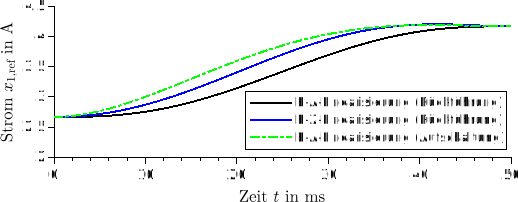
\includegraphics[width=0.8\textwidth]{Hochsetzsteller_Tracking_Strom}
\par\end{centering}
\caption{Ausgangsreferenzverläufe des Hochsetzstellers\label{fig:Hochsetzsteller-Tracking-Strom-FB-FF}}
\end{figure}


\section{Modellbasierte Regelung (IMC)\label{sec:Modellbasierte-Regelung-IMC}}

Die in diesem Buch behandelten Regelungsansätze sind alle modellbasiert
in dem Sinne, dass das Modell der Regelstrecke für den Reglerentwurf
benötigt wird.\footnote{Im Unterschied zu modellbasierten Verfahren gibt es auch Ansätze zur
\emph{modellfreien} Steuerung bzw. Regelung~\cite{fliess2009}. Bei
diesen Verfahren werden nur die Mess- oder Simulationsdaten genutzt.} Bei der \emph{modellbasierten Regelung}\index{modellbasierte Regelung}
(engl. \emph{internal model control}, kurz \emph{IMC}) im engeren
Sinne ist das Modell der Regelstrecke unmittelbar im Regler enthalten.
Der eigentliche Reglerentwurf ist auch bei komplizierten Modellen
vergleichsweise einfach und ähnelt der Entwurf einer Steuerung. Daher
ist dieser Ansatz u.\,a. in der chemischen Verfahrenstechnik sehr
beliebt. In Abschnitt~\ref{subsec:Modellbasierte-Regelung-linear}
wird zunächst der Reglerentwurf für lineare Regelstrecken vorgestellt~\cite{garcia1982}.
Die Verallgemeinerung auf nichtlineare Regelstrecken erfolgt in Abschnitt~\ref{subsec:Modellbasierte-Regelung-nichtlinear-minimalphasig}.

\subsection{Modellbasierte Regelung für lineare Systeme\label{subsec:Modellbasierte-Regelung-linear}}

Die Regelstrecke werde im Laplace-Bereich durch 
\[
Y(s)=G(s)\,U(s)+D(s)
\]
mit einer gebrochen rationalen, properen\index{Ubertragungsfunktion@{\"U}bertragungsfunktion!proper}\footnote{Eine rationale Übertragungsfunktion heißt \emph{proper}, wenn der
Grad des Zählerpolynoms nicht größer ist als der Grad des Nennerpolynoms.} Übertragungsfunktion~$G$, dem Eingang~$U$, dem Ausgang~$Y$
und der Störung~$D$ beschrieben. Abb.~\ref{fig:Struktur-IMC-linear}
zeigt die bei der modellbasierten Regelung verwendete Anordnung~\cite{lunze2007}.
Der Gesamtregeler besteht dabei aus einem sog. \emph{IMC-Regler} mit
der Übertragungsfunktion~$K$ und einem durch die Übertragungsfunktion~$\hat{G}$
beschriebenen Modell der Regelstrecke.
\begin{figure}
\begin{centering}
\resizebox{0.75\textwidth}{!}{\input{IMC-linear.pdftex_t}}
\par\end{centering}
\caption{Struktur einer modellbasierten Regelung\label{fig:Struktur-IMC-linear}}
\end{figure}

Bei der modellbasierten Regelung wird der Streckenausgang~$y$ mit
dem Modellausgang~$\hat{y}$ verglichen. Bei exakter Modellkenntnis
($G=\hat{G}$) reduziert sich im störungsfreien Fall ($d=0$) der
in Abb.~\ref{fig:Struktur-IMC-linear} gezeigte Regelkreis wegen
$y=\hat{y}$ auf eine reine Steuerung, wobei der IMC-Regler als Steuerungseinrichtung
bzw. Vorfilter fungiert (siehe Abb.~\ref{fig:Struktur-IMC-Steuerung}).
Für die Stabilität des Gesamtsystems ergibt sich sofort die Forderung,
dass sowohl die Regelstrecke als auch der Regler stabil sein müssen. 

\begin{figure}
\begin{centering}
\resizebox{0.65\textwidth}{!}{\input{IMC-linear-Steuerung.pdftex_t}}
\par\end{centering}
\caption{Vereinfachung einer modellbasierten Regelung zur Steuerung\label{fig:Struktur-IMC-Steuerung}}
\end{figure}

Bei der Steuerung in Abb.~\ref{fig:Struktur-IMC-Steuerung} würde
man mit der Wahl 
\begin{equation}
K(s)=G^{-1}(s)\label{eq:IMC-perfekter-Regler-linear}
\end{equation}
die Dynamik der Regelstrecke exakt kompensieren. Der Ausgang~$y$
würde (nach dem einmaligen Einschwingen durch verschiedene Anfangswerte
von Strecke und Steuerung) der Führungsgröße unmittelbar folgen. Man
spricht daher von einem \emph{perfekten} \emph{IMC-Regler}~\cite{garcia1982}.
Der perfekte Regler~(\ref{eq:IMC-perfekter-Regler-linear}) ist jedoch
aus folgenden Gründen meistens nicht einsetzbar:
\begin{enumerate}
\item \label{enu:IMC-Problem1}Ist der Zählergrad der Streckenübertragungsfunktion~$G$
echt kleiner als der Nennergrad, dann sind die Verhältnisse bei der
inversen Übertragungsfunktion~$G^{-1}$ umgekehrt, so dass der Zählergrad
größer als der Nennergrad ist. Eine derartige Reglerübertragungsfunktion~(\ref{eq:IMC-perfekter-Regler-linear})
wäre nicht mehr proper. 
\item \label{enu:IMC-Problem2}Bei der Inversion~(\ref{eq:IMC-perfekter-Regler-linear})
gehen die Nullstellen von~$G$ in die Polstellen von~$G^{-1}$ über.
Liegen Nullstellen von~$G$ in der rechten Halbebene, dann besitzt
das inverse Modell~$G^{-1}$ Polstellen in der rechten Halbebene
und ist daher instabil.
\end{enumerate}

Das erste Problem lässt sich umgehen, wenn man den IMC-Regler zusätzlich
mit einem Filter ausstattet. Sei $r>0$ die Differenz zwischen Zähler-
und Nennergrad von~$G$, d.\,h. das durch die Übertragungsfunktion~$G$
beschriebene Modell hat den relativen Grad~$r$ (vgl. Anmerkung~\ref{rem:rel-grad-Uebertragungsfunktion}).
Setzt man für das Filter die Übertragungsfunktion
\begin{equation}
F(s)=\frac{a_{0}}{a_{0}+a_{1}s+\cdots+a_{r-1}s^{r-1}+s^{r}}\label{eq:IMC-Filter-F}
\end{equation}
mit einem stabilen Nennerpolynom an, so ist der neue IMC-Regler
\begin{equation}
K(s)=F(s)\cdot G^{-1}(s)\label{eq:IMC-Regler-mit-Filter-linear}
\end{equation}
proper, d.\,h. der Zähler von~$K$ weist keinen Gradüberschuss mehr
auf. 

Eine stabile Übertragungsfunktion
\begin{equation}
G(s)=\frac{Z(s)}{N(s)}=\frac{\bar{b}_{0}+\bar{b}_{1}s+\bar{b}_{2}s^{2}+\cdots+\bar{b}_{n-r}s^{n-r}}{\bar{a}_{0}+\bar{a}_{1}s+\cdots+\bar{a}_{n-1}s^{n-1}+s^{n}}\label{eq:IMC-P}
\end{equation}
nennt man \emph{minimalphasig}\footnote{Die Verbindung zur Minimalphasigkeit in Sinne der Nulldynamik wird
in Anmerkung~\ref{rem:Nulldynamik-Nullstellen-Uebertragungsfunktion}
beschrieben.}\index{Ubertragungsfunktion@{\"U}bertragungsfunktion!minimalphasig}\index{minimalphasig},
wenn alle Nullstellen des Zählerpolynoms $Z(s)$ in der offenen linken
Halbebene liegen. Für eine minimalphasige Streckenübertragungsfunktion
ist der IMC-Regler~(\ref{eq:IMC-Regler-mit-Filter-linear}) auch
stabil. Andernfalls kann man die Übertragungsfunktion~$G$ in einen
minimalphasigen Anteil~$G_{\text{MP}}$ und einen Allpass~$G_{\text{A}}$
zerlegen~\cite{lunze2007}:
\begin{equation}
G(s)=G_{\text{MP}}(s)\cdot G_{\text{A}}(s).\label{eq:zerlegung-minimalphasig-allpass}
\end{equation}
Der IMC-Regler hat dann die Form
\begin{equation}
K(s)=F(s)\cdot G_{\text{MP}}^{-1}(s).\label{eq:IMC-Regler-mit-Filter-minimalphasig}
\end{equation}
Diesen Ansatz kann man als stabile Approximation der inversen Strecken\-dynamik~(\ref{eq:IMC-perfekter-Regler-linear})
auffassen.

\begin{remark}
\label{rem:Uebertragungsfunktion-minimalphasiger-Anteil}Bei einer
nicht minimal\-phasigen Übertragungsfunktion~$G$ erhält man den
minimal\-phasigen Anteil~$G_{\text{MP}}$ dadurch, dass man die
in der rechten Halbebene liegenden Nullstellen an der imaginären Achse
spiegelt. Da die Nullstellen entweder reell sind oder in konjugiert
komplexen Paaren auftreten, kann diese Spiegelung auch am Ursprung
erfolgen. Liegen \textit{alle} Nullstellen in der rechten Halbebene,
so heißt die Übertragungsfunktion \emph{maximal\-phasig}\index{Ubertragungsfunktion@{\"U}bertragungsfunktion!maximalphasig}\index{maximalphasig}~\cite{doyle96}.
In diesem Fall erhält man für die Übertragungsfunktion~(\ref{eq:IMC-P})
den minimal\-phasigen Anteil 
\begin{equation}
G_{\text{MP}}(s)=\frac{Z(-s)}{N(s)}=\frac{\bar{b}_{0}-\bar{b}_{1}s+\bar{b}_{2}s^{2}-\cdots+\bar{b}_{n-r}(-s)^{n-r}}{\bar{a}_{0}+\bar{a}_{1}s+\cdots+\bar{a}_{n-1}s^{n-1}+s^{n}},\label{eq:IMC-PMP}
\end{equation}
durch die Substitution $s\mapsto-s$ im Zählerpolynom.
\end{remark}

\begin{example}
\label{exa:IMC-linear}Die Übertragungsfunktion
\[
G(s)=\frac{3-s}{(s+1)(s+2)}
\]
der Regelstrecke ist selber stabil, ihre Inverse~$G^{-1}$ wegen
der o.\,g. Probleme~\ref{enu:IMC-Problem1} und~\ref{enu:IMC-Problem2}
dagegen nicht. Eine Zerlegung nach Gl.~(\ref{eq:zerlegung-minimalphasig-allpass})
liefert 
\[
G(s)=\underbrace{\frac{3+s}{(s+1)(s+2)}}_{{\displaystyle G_{\text{MP}}(s)}}\cdot\frac{3-s}{3+s}.
\]
Der Gradunterschied zwischen Nenner- und Zählerpolynom erfordert ein
Filter~(\ref{eq:IMC-Filter-F}) der Ordnung $r=1$. Damit erhält
man für den IMC-Regler~(\ref{eq:IMC-Regler-mit-Filter-minimalphasig})
die stabile Übertragungsfunktion
\[
K(s)=\frac{a_{0}}{s+a_{0}}\cdot\frac{(s+1)(s+2)}{3+s}
\]
mit einem Koeffizienten $a_{0}>0$.\footnote{Mit $a_{0}\in\{1,2\}$ kann man durch Pol-Nullstellen-Kürzung die
Ordnung des IMC-Reglers reduzieren. Für $a_{0}=1$ erhält man beispielsweise
$K(s)=\frac{s+2}{s+3}$.}
\end{example}

Die in Abb.~\ref{fig:Struktur-IMC-linear} gezeigte Anordnung einer
modellbasierten Regelung kann man in die Form eines Standardregelkreises
überführen (siehe Abb.~\ref{fig:IMC-linear-Standardregelkreis}).
Die gezeigte Regel\-kreis\-struktur lässt sich in ähnlicher Weise
auf nichtlineare Systeme übertragen.

\begin{figure}
\begin{centering}
\resizebox{0.8\textwidth}{!}{\input{IMC-linear-Standardregelkreis.pdftex_t}}
\par\end{centering}
\caption{Darstellung der modellbasierten Regelung als Standardregelkreis\label{fig:IMC-linear-Standardregelkreis}}
\end{figure}


\subsection{Modellbasierte Regelung für nichtlineare minimalphasige Systeme\label{subsec:Modellbasierte-Regelung-nichtlinear-minimalphasig}}

Das Konzept der modellbasierten Regelung lässt sich auf nichtlineare
Systeme verallgemeinern~\cite{economou1986,henson1991,schwarzmann2006,schwarzmann2007}.
Wir betrachten ein System~(\ref{eq:var-basissystem}) mit relativem
Grad~$r$. Das System sei minimalphasig und eingangs-zustands-stabil
(siehe Anhang~\ref{sec:Stabilitaet-erregter-Systeme}). 

Bei wohldefiniertem relativen Grad kann man das inverse Systemmodell
durch die Hirschorn-Inverse~(\ref{eq:hirschorn-inverse-SISO})\index{Hirschorn-Inverse}
realisieren (vgl. Anmerkung~\ref{rem:Hirschorn-Inverse}). Die Hirschorn-Inverse
benötigt neben der $r$-ten Zeitableitung des Ausgangs auch den Systemzustand.
Geht man zunächst von einer Systemdarstellung in der Byrnes-Isidori-Normalform~(\ref{eq:var-BI-NF})
aus, so ist auch der Zustand~$\xi$ des ersten Teilsystems nach Gl.~(\ref{eq:Zustand-xi-durch-y})
durch die Zeitableitungen des Ausgangs~$y$ darstellbar. Da Zeitableitungen
aus Mess\-signalen schwer zu ermitteln sind, schalten wir dem inversen
Systemmodell in Anlehnung an Gl.~(\ref{eq:IMC-Regler-mit-Filter-linear})
ein Filter vor. Die Übertragungsfunktion~(\ref{eq:IMC-Filter-F})
wird dabei als Zustandsraummodell 
\begin{equation}
\left.\begin{array}{lcl}
\dot{\hat{\xi}}_{1} & = & \hat{\xi}_{2}\\
 & \vdots\\
\dot{\hat{\xi}}_{r-1} & = & \hat{\xi}_{r}\\
\dot{\hat{\xi}}_{r} & = & -a_{0}\hat{\xi}_{1}-\cdots-a_{r-1}\hat{\xi}_{r}+a_{0}\tilde{w}\\
\hat{y} & = & \hat{\xi}_{1}
\end{array}\right\} \quad\begin{array}{lcl}
\dot{\hat{\xi}} & = & \left(A-bk^{T}\right)\hat{\xi}+a_{0}b\,\tilde{w}\\
\hat{y} & = & c^{T}\hat{\xi}
\end{array}\label{eq:IMC-Zustandsvariablenfilter}
\end{equation}
mit $k=(a_{0},\ldots,a_{r-1})^{T}$ implementiert, so dass sich der
Modellausgang~$\hat{y}$ und seine Zeitableitungen aus 
\[
\hat{y}=\hat{\xi}_{1},\;\dot{\hat{y}}=\hat{\xi}_{2},\;\ldots,\;\hat{y}^{(r-1)}=\hat{\xi}_{r},\;\hat{y}^{(r)}=-a_{0}\hat{\xi}_{1}-\cdots-a_{r-1}\hat{\xi}_{r}+a_{0}\tilde{w}
\]
ergeben. Man spricht hierbei von einem \emph{Zustandsvariablenfilter}\index{Zustandsvariablenfilter}~\cite{isermann2}.
Dabei wird aus dem Referenzsignal~$\tilde{w}$ ein geglätteter Zeitverlauf~$\hat{y}$
generiert, den man wie einen Referenzausgang aus Abschnitt~\ref{sec:Trajektorienfolgeregelung-Feedback}
behandeln kann. Den von dem Filter~(\ref{eq:IMC-Zustandsvariablenfilter})
bereitgestellten Zustand~$\hat{\xi}$ speist man in das zweite Teilsystem
der Byrnes-Isidori-Normalform
\[
\dot{\hat{\eta}}=q(\hat{\xi},\hat{\eta})
\]
ein und erhält damit einen Referenzverlauf~$\hat{\eta}$. Aus der
letzten Zeile des ersten Teilsystems erhält man den Eingang 
\begin{equation}
u=\frac{1}{\beta(\hat{\xi},\hat{\eta})}\left(\hat{y}^{(r)}-\alpha(\hat{\xi},\hat{\eta})\right).\label{eq:IMC-u}
\end{equation}
Mit der Rücktransformation $\hat{x}=\Phi^{-1}(\hat{\xi},\hat{\eta})$
kann man~(\ref{eq:IMC-u}) auch in Originalkoordinaten darstellen
und erhält dabei die Hirschorn-Inverse~(\ref{eq:hirschorn-inverse-SISO}).

Verwendet man anstelle der Byrnes-Isidori-Normalform~(\ref{eq:var-BI-NF})
die in der Regel leichter zu berechnende Eingangs-Ausgangs-Normalform~(\ref{eq:var-EA-NF}),
dann muss man erst den Eingang nach Gl.~(\ref{eq:IMC-u}) berechnen
und dann in das zweite Teilsystem einsetzen: 
\begin{equation}
\dot{\hat{\eta}}=q(\hat{\xi},\hat{\eta})+d(\hat{\xi},\hat{\eta})u.\label{eq:IMC-TS2-EA}
\end{equation}

Gleichungen~(\ref{eq:IMC-Zustandsvariablenfilter}), (\ref{eq:IMC-u})
und~(\ref{eq:IMC-TS2-EA}) bilden den IMC-Regler. Der Modell\-ausgang~$\hat{y}$
liegt dabei schon am Filter~(\ref{eq:IMC-Zustandsvariablenfilter})
an, so dass das Streckenmodell nicht noch separat zu implementieren
ist. Abb.~\ref{fig:Regelkreis-IMC-nichtlinear} zeigt den Regelkreis
für das nichtlineare System~(\ref{eq:var-basissystem}) in Verallgemeinerung
von Abb.~\ref{fig:IMC-linear-Standardregelkreis}. 

\begin{figure}
\begin{centering}
\resizebox{1\textwidth}{!}{\input{IMC-nichtlinear.pdftex_t}}
\par\end{centering}
\caption{Regelkreis mit nichtlinearem IMC-Regler für eine minimalphasige Regelstrecke\label{fig:Regelkreis-IMC-nichtlinear}}

\end{figure}

\begin{example}
\label{exa:hochsetzsteller-IMC}Wir betrachten wieder den \index{Hochsetzsteller}Hochsetzsteller~(\ref{eq:var-hochsetzsteller})
mit dem Strom als Ausgang entsprechend Gl.~(\ref{eq:hochsetzsteller-ausgang-strom-tracking}).
Das System hat den relativen Grad $r=1$ und liegt schon in der Eingangs-Ausgangs-Normalform~(\ref{eq:var-EA-NF})
mit $\xi_{1}=x_{1}$ und $\eta_{1}=x_{2}$ vor. In der Implementierung
bietet sich daher die Verwendung der ursprünglichen Bezeichnungen
für die Zustandsvariablen an. Das Zustandsvariablenfilter~(\ref{eq:IMC-Zustandsvariablenfilter})
wird als Filter erster Ordnung
\begin{equation}
\dot{\hat{x}}_{1}=a_{0}\left(\tilde{w}-\hat{x}_{1}\right),\quad\tilde{w}=w-\left(y-\hat{x}_{1}\right)\label{eq:hochsetzsteller-IMC-x1hat}
\end{equation}
mit einem Koeffizienten $a_{0}>0$ angesetzt. Das Umstellen der ersten
Systemgleichung von~(\ref{eq:var-hochsetzsteller}) liefert die Hirschorn-Inverse
\begin{equation}
u=\frac{\hat{x}_{2}-E+L\dot{\hat{x}}_{1}}{\hat{x}_{2}}\label{eq:hochsetzsteller-IMC-u}
\end{equation}
nach Gl.~(\ref{eq:IMC-u}). Das damit erzeugte Eingangssignal speist
man in die zweite Systemgleichung von~(\ref{eq:var-hochsetzsteller})
ein, um den Verlauf von~$x_{2}$ im Regler zu simulieren: 
\begin{equation}
\dot{\hat{x}}_{2}=(1-u)\frac{1}{C}\hat{x}_{1}-\frac{1}{RC}\hat{x}_{2}.\label{eq:hochsetzsteller-IMC-x2hat}
\end{equation}
Gleichzeitig ist~(\ref{eq:hochsetzsteller-IMC-u}) das Reglerausgangssignal,
welches in die Regelstrecke~(\ref{eq:var-hochsetzsteller}) eingespeist
wird.

Für die numerische Simulation wird wieder der Übergang von $20\,\text{V}$
auf $25\,\text{V}$ betrachtet. Dazu wird das Führungssignal 
\[
w(t)=\left\{ \begin{array}{rcl}
2,\bar{6}\,\text{A} & \text{für} & t<50\,\text{ms}\\
4,1\bar{6}\,\text{A} & \text{für} & t\geq50\,\text{ms}
\end{array}\right.
\]
vorgegeben. Für den Hochsetzsteller werden die von der Ruhelage abweichenden
Anfangswerte $x_{1}(0)=2\,\text{A}$ und $x_{2}(0)=15\,\text{V}$
vorgegeben, für den aus den Differentialgleichungen~(\ref{eq:hochsetzsteller-IMC-x1hat})
und~(\ref{eq:hochsetzsteller-IMC-x2hat}) bestehenden IMC-Regler
dagegen die Anfangswerte $\hat{x}_{1}(0)=2,\bar{6}\,\text{A}$ und
$\hat{x}_{2}(0)=20\,\text{\text{V}}$. Wie in Abschnitt~\ref{subsec:Hochsetzsteller-Num-Sim}
wird der normierte Filterparameter $a_{0}=300$ eingesetzt. Abb.~\ref{fig:Hochsetzsteller-IMC-Strom}
zeigt das Simulationsergebnis. Durch die unterschiedlichen Anfangswerte~$x(0)$
bzw.~$\hat{x}(0)$ treten zunächst Schwingungen auf, die bei dem
ab $t=50\,\text{ms}$ eingeleiteten Übergang der Ausgangsspannung
weitgehend abgeklungen sind.
\end{example}
\begin{figure}
\begin{centering}
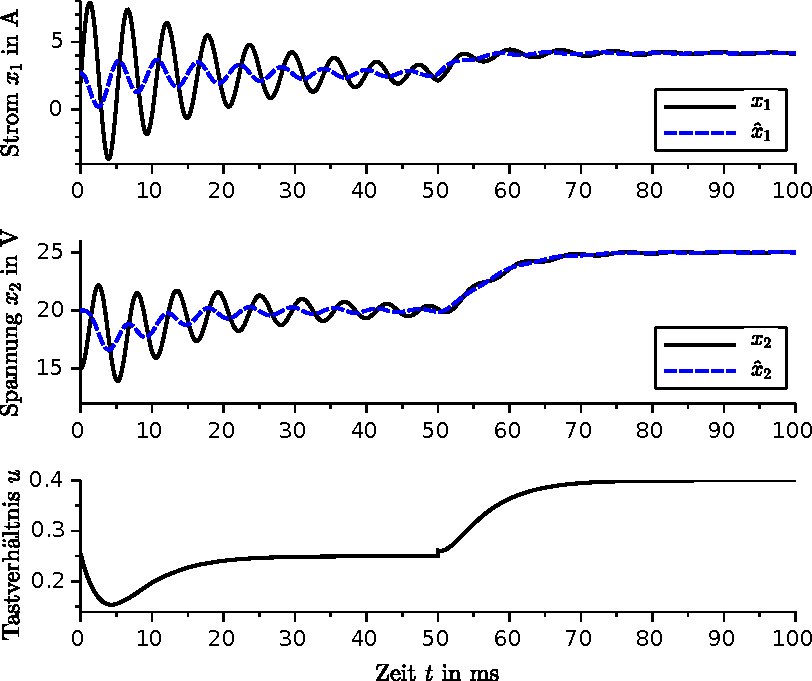
\includegraphics[width=0.8\textwidth]{Hochsetzsteller_IMC_Strom}
\par\end{centering}
\caption{Simulation des Hochsetzstellers mit dem IMC-Regler aus Beispiel~\ref{exa:hochsetzsteller-IMC}\label{fig:Hochsetzsteller-IMC-Strom}}
\end{figure}


\subsection{Modellbasierte Regelung für nichtlineare maximalphasige Systeme\label{subsec:Modellbasierte-Regelung-nichtlinear-maximalphasig}}

Die zur IMC-Regelung verwendete Aufspaltung einer nicht minimalphasigen
Übertragungsfunktion in einen minimalphasigen Anteil und einen Allpass
lässt sich prinzipiell auch auf nichtlineare Systeme übertragen, ist
in der Regel aber sehr kompliziert~\cite{ball2004}. In Anlehnung
an~\cite{doyle96} wird in diesem Abschnitt eine Methode zur IMC-Regelung
einer speziellen Klasse nicht minimalphasiger Systeme vorgestellt.

Wir betrachten ein System~(\ref{eq:var-basissystem}) mit einem wohldefinierten
relativen Grad $r<n$. Damit kann das Systm in die Byrnes-Isidori-Normalform~(\ref{eq:var-BI-NF})
transformiert werden. Das System ist minimalphasig\index{minimalphasig},
wenn die Ruhelage $\eta=0$ der Nulldynamik
\begin{equation}
\dot{\eta}=q(0,\eta)\label{eq:var-nulldynamik}
\end{equation}
asymptotisch stabil ist (vgl. Abschnitt~\ref{subsec:Reglerentwurf-zur-Stabilisierung-Ruhelage}).
Ist die Ruhelage zusätzlich hyperbolisch\index{Ruhelage!hyperbolische},
dann liegen alle $n-r$ Eigenwerte der aus der Taylor-Linearisierung
resultierenden Matrix 
\begin{equation}
A_{22}:=\left.\frac{\partial}{\partial\eta}q(0,\eta)\right|_{\eta=0}\label{eq:eq:var-nulldynamik-linearisierung}
\end{equation}
in der offenen linken Halbebene (vgl. Anmerkungen~\ref{rem:Nulldynamik-linear}
und~\ref{rem:Nulldynamik-Nullstellen-Uebertragungsfunktion}).

In Anlehnung an~\cite{doyle96} nennen wir ein System \emph{maximalphasig}\index{maximalphasig},
wenn die Ruhelage $\eta=0$ des zur Nulldynamik~(\ref{eq:var-nulldynamik})
assoziierten Systems 
\begin{equation}
\dot{\eta}=-q(0,\eta)\label{eq:nulldynamik-maximalphasig}
\end{equation}
asymptotisch stabil ist. Im Falle einer hyperbolischen Ruhelage liegen
dann alle Eigenwerte der zugehörigen Jacobimatrix
\[
\left.\frac{\partial}{\partial\eta}\left(-q(0,\eta)\right)\right|_{\eta=0}=-\left.\frac{\partial}{\partial\eta}q(0,\eta)\right|_{\eta=0}=-A_{22}
\]
in der offenen linken Halbebene. Das bedeutet, dass alle Eigenwerte
der Jacobi\-matrix~(\ref{eq:eq:var-nulldynamik-linearisierung})
der ursprünglichen Nulldynamik~(\ref{eq:var-nulldynamik}) in der
offenen rechten Halbebene liegen.

Zusätzlich zur Byrnes-Isidori-Normalform betrachten wir das System~(\ref{eq:var-basissystem})
in der verallgemeinerten Regelungsnormalform\index{verallgemeinerte Regelungsnormalform}\index{Normalform!verallgemeinerte Regelungs-}
\begin{equation}
\begin{array}{lcl}
\dot{z}_{1} & = & z_{2}\\
 & \vdots\\
\dot{z}_{n-1} & = & z_{n}\\
\dot{z}_{n} & = & \underbrace{\alpha\left(z,u,\dot{u},\ddot{u},\ldots,u^{(n-r-1)}\right)+\beta\left(z,u,\dot{u},\ddot{u},\ldots,u^{(n-r-1)})\right)u^{(n-r)}}_{{\displaystyle \delta\left(u,\dot{u},\ldots,u^{(n-r)}\right)}}\\
y & = & z_{1},
\end{array}\label{eq:var-verallgemeinerte-Regelungsnormalform-maxmalphasig}
\end{equation}
vgl. Abschnitt~\ref{subsec:Verallgemeinerte-Regelungsnormalform}.
Da das Ausgangssystem~(\ref{eq:var-basissystem}) affin ist, ist
die in der letzten Differentialgleichung von~(\ref{eq:var-verallgemeinerte-Regelungsnormalform-maxmalphasig})
auftretende Nichtlinearität~$\delta$ affin bezüglich der höchsten
Zeitableitung des Eingangs. Die Transformation $z=\Phi(x,u,\dot{u},\ldots,u^{(n-r-1)})$
ergibt sich aus Zeitableitungen $z_{1}=y,\,z_{2}=\dot{y},\,z_{3}=\ddot{y},\ldots,\,z_{n}=y^{(n-1)}$.

Die Linearierung von System~(\ref{eq:var-verallgemeinerte-Regelungsnormalform-maxmalphasig})
führt auf eine Übertragungsfunktion~$G(s)$ der Form~(\ref{eq:IMC-P}).
Die Koeffizienten $\bar{b}_{0},\ldots,\bar{b}_{n-r}$ des Zählerpolynoms
$Z(s)$ ergeben sich dabei aus den partiellen Ableitungen von~$\delta$
nach dem Eingang und seien Zeitableitungen, d.\,h. 
\begin{equation}
\bar{b}_{0}=\frac{\partial\delta}{\partial u},\;\bar{b}_{1}=\frac{\partial\delta}{\partial\dot{u}},\;\ldots,\bar{b}_{n-r}=\frac{\partial\delta}{\partial u^{(n-r)}}\label{eq:IMC-koeff-nennerpolynom}
\end{equation}
für $z=0,u=0,\ldots,u^{(n-r)}=0$. Bei einem maximalphasigen System
mit hyperbolischer Ruhelage liegen alle Nullstellen des Zählerpoylnoms
$Z(s)$ in der rechten Halbebene. Der Übergang von $Z(s)$ zu $Z(-s)$
liefert den minimalphasigen Anteil~(\ref{eq:IMC-PMP}) der Übertragungsfunktion~(\ref{eq:IMC-P}),
vgl. Anmerkung~\ref{rem:Uebertragungsfunktion-minimalphasiger-Anteil}.
Diesen Ansatz übertragen wir jetzt auf das nichtlineare System~(\ref{eq:var-verallgemeinerte-Regelungsnormalform-maxmalphasig}).
Die im Zählerpolynom der Übertragungsfunktion durchgeführte Ersetzung
$s\mapsto-s$ entspricht wegen~(\ref{eq:IMC-koeff-nennerpolynom})
in der Nichtlinearität~$\delta$ der Substitution $\tfrac{\d}{\d t}\mapsto-\tfrac{\d}{\d t}$.
Im Falle eines maximalphasigen Systems~(\ref{eq:var-verallgemeinerte-Regelungsnormalform-maxmalphasig})
erhält man dadurch den zugehörigen minimalphasigen Anteil
\begin{equation}
\begin{array}{lcl}
\dot{z}_{1} & = & z_{2}\\
 & \vdots\\
\dot{z}_{n-1} & = & z_{n}\\
\dot{z}_{n} & = & \alpha\left(z,u,-\dot{u},\ddot{u},\ldots,(-1)^{n-r-1}u^{(n-r-1)}\right)\\
 &  & +(-1)^{n-r}\beta\left(z,u,-\dot{u},\ddot{u},\ldots,(-1)^{n-r-1}u^{(n-r-1)}\right)u^{(n-r)}\\
y & = & z_{1}.
\end{array}\label{eq:var-verallgemeinerte-Regelungsnormalform-minimalphasig}
\end{equation}
Die Lineariserung des resultierenden minimalphasigen Systems~(\ref{eq:var-verallgemeinerte-Regelungsnormalform-minimalphasig})
liefert unmittelbar die Übertragungsfunktion $G_{\text{MP}}(s)$ analog
zu Gl.~(\ref{eq:IMC-PMP}):

\[
\begin{CD}
\text{System}~\eqref{eq:var-verallgemeinerte-Regelungsnormalform-maxmalphasig} @>{\displaystyle\text{Zerlegung}}>>\text{System}~\eqref{eq:var-verallgemeinerte-Regelungsnormalform-minimalphasig}\\
@V{\displaystyle\text{Linearisierung}}VV @VV{\displaystyle\text{Linearisierung}}V\\
G(s) @>>{\displaystyle\text{Zerlegung}}> G_\text{MP}(s)
\end{CD}
\]

Zur Verallgemeinerung des linearen IMC-Reglers~(\ref{eq:IMC-Regler-mit-Filter-minimalphasig})
auf den nichtlinearen Fall lösen wir die letzte Differentialgleichung
von~(\ref{eq:var-verallgemeinerte-Regelungsnormalform-minimalphasig})
unter Beachtung von $\dot{z}_{n}=y^{(n)}$ nach der höchsten Zeitableitung
des Eingangs auf:
\begin{equation}
u^{(n-r)}=\left(-1\right)^{n-r}\,\frac{y^{(n)}-\alpha\left(z,u,-\dot{u},\ddot{u},\ldots,(-1)^{n-r-1}u^{(n-r-1)}\right)}{\beta\left(z,u,-\dot{u},\ddot{u},\ldots,(-1)^{n-r-1}u^{(n-r-1)}\right)u^{(n-r)}}.\label{eq:IMC-max-inv}
\end{equation}
Der Zustand~$z$ und die Zeitableitung~$y^{(n)}$ werden durch ein
Zustandsvariablenfilter der Struktur~(\ref{eq:IMC-Zustandsvariablenfilter}),
aber der Ordnung~$n$, mit dem Zustand~$\hat{z}$ geschätzt:
\begin{equation}
\begin{array}{lcl}
\dot{\hat{z}} & = & \left(A-bk^{T}\right)\hat{z}+a_{0}b\,\tilde{w}\\
\hat{y} & = & c^{T}\hat{z}.
\end{array}\label{eq:Filter-maximalphasig}
\end{equation}
Die so erhaltenen Schätzgrößen setzt man in Gl.~(\ref{eq:IMC-max-inv})
ein. Die Ableitung~$u^{(n-r)}$ führt man einer Integratorkette der
Länge $n-r$ zu, womit man die in Gl.~(\ref{eq:IMC-max-inv}) benötigten
Ableitungen $u^{(n-r-1)},\ldots,\dot{u}$ und auch den Eingang~$u$
als Stellgröße für die Regelstrecke~(\ref{eq:var-basissystem}) erhält.
Das dadurch entstehende Regelungsschema ist in Abb.~\ref{fig:Regelkreis-IMC-maximalphasig}
dargestellt.

\begin{figure}
\begin{centering}
\resizebox{1\textwidth}{!}{\input{IMC-maximalphasig.pdftex_t}}
\par\end{centering}
\caption{Regelkreis mit IMC-Regler eine für maximalphasige Regelstrecke\label{fig:Regelkreis-IMC-maximalphasig}}
\end{figure}

\begin{example}
\label{exa:Hochsetzsteller-IMC-Spannung}\index{Hochsetzsteller}Betrachtet
wird wieder der Hochsetzsteller. Wir verwenden die Kondensatorspannung~$x_{2}$
gleichzeitig als Ausgang wie auch als erste Koordinate des transformierten
Systems:
\begin{equation}
z_{1}=y=h(x)=x_{2}.\label{eq:IMC-hochsetzsteller-ausgang-spannung}
\end{equation}
Die zweite Koordinate ist die Zeitableitung des Ausgangs
\begin{equation}
z_{2}=\dot{y}=L_{f}h(x)+L_{g}h(x)u=(1-u)\frac{1}{C}x_{1}-\frac{1}{RC}x_{2},\label{eq:IMC-hochsetzsteller-ausgangsableitung}
\end{equation}
die vom Eingang~$u$ abhängt, so dass das System den relativen Grad
$r=1$ besitzt. Gln.~(\ref{eq:IMC-hochsetzsteller-ausgang-spannung})
und~(\ref{eq:IMC-hochsetzsteller-ausgangsableitung}) bilden eine
vom Eingang abhängige Koordinatentransformation $z=\Phi(x,u)$ mit
der Rücktransformation
\[
x_{1}=-\frac{z_{1}+RCz_{2}}{(u-1)R},\quad x_{2}=z_{1}.
\]
Aus der zweiten Zeitableitung des Ausgangs
\begin{eqnarray*}
\ddot{y} & = & L_{f}^{2}h(x)+\left(L_{g}L_{f}h(x)+L_{f}L_{g}h(x)\right)u+L_{g}^{2}h(x)u^{2}+L_{g}h(x)\dot{u}\\
 & = & -\frac{-Lx_{2}-\left(u-1\right)x_{1}LR+\left(L\dot{u}x_{1}+uE-E+u^{2}x_{2}-2ux_{2}+x_{2}\right)CR^{2}}{C^{2}LR^{2}}\\
 & = & \underbrace{-\frac{Lz_{2}+\left(u-1\right)\left(E+\left(u-1\right)\,z_{1}\right)R}{CLR}}_{{\displaystyle \alpha(z,u)}}+\underbrace{\frac{z_{1}+RCz_{2}}{(u-1)RC}}_{{\displaystyle \beta(z,u)}}\dot{u}
\end{eqnarray*}
erhält man die letzte Zeile der verallgemeinerten Regelungsnormalform:
\begin{equation}
\begin{array}{lcl}
\dot{z}_{1} & = & z_{2}\\
\dot{z}_{2} & = & \alpha(z,u)+\beta(z,u)\,\dot{u}\\
y & = & z_{1}
\end{array}\label{eq:hochsetzsteller-verallg-RNF1}
\end{equation}
Durch Zeitumkehr in der Eingangsdynamik, d.\,h. $\dot{u}\mapsto-\dot{u}$,
geht das nicht\-minimal\-phasige System~(\ref{eq:hochsetzsteller-verallg-RNF1})
in die minimalphasige Approximation
\begin{equation}
\begin{array}{lcl}
\dot{z}_{1} & = & z_{2}\\
\dot{z}_{2} & = & \alpha(z,u)-\beta(z,u)\,\dot{u}\\
y & = & z_{1}
\end{array}\label{eq:hochsetzsteller-verallg-RNF2}
\end{equation}
über. Stellt man die letzte Differentialgleichung in~(\ref{eq:hochsetzsteller-verallg-RNF2})
nach~$\dot{u}$ um, so erhält man 
\begin{equation}
\dot{u}=-\frac{\left(u-1\right)\left(z_{2}L+\left(\dot{z}_{2}CL+uE-E+u^{2}z_{1}-2uz_{1}+z_{1}\right)R\right)}{L\left(z_{2}CR+z_{1}\right)}.\label{eq:hochsetzsteller-maximalphasig-du}
\end{equation}
Die Größen $z_{1},z_{2},\dot{z}_{2}$ lassen sich durch $y,\dot{y},\ddot{y}$
repräsentieren. Im IMC-Regler verwendet man dafür die vom Zustandsvariablenfilter
\begin{equation}
\begin{array}{lcl}
\dot{\hat{z}}_{1} & = & \hat{z}_{2}\\
\dot{\hat{z}}_{2} & = & -a_{0}\hat{z}_{1}-a_{1}\hat{z}_{2}+a_{0}\tilde{w}\\
\hat{y} & = & \hat{z}_{1}
\end{array}\label{eq:hochsetzsteller-maxphas-zustandsvarfilter}
\end{equation}
mit $a_{0},a_{1}>0$ generierten Schätzsignale $\hat{y},\dot{\hat{y}},\ddot{\hat{y}}$.
Die Integration von~$\dot{u}$ aus Gl.~(\ref{eq:hochsetzsteller-maximalphasig-du})
liefert das Streckeneingangssignal~$u$. Mit~(\ref{eq:hochsetzsteller-maximalphasig-du})
und~(\ref{eq:hochsetzsteller-maxphas-zustandsvarfilter}) erhält
man insgesamt einen dynamischen Regler dritter Ordnung.

Für die numerische Simulation wird der Übergang von $20\,\text{V}$
auf $25\,\text{V}$ direkt durch das Führungssignal 
\[
w(t)=\left\{ \begin{array}{rcl}
20\,\text{V} & \text{für} & t<50\,\text{ms}\\
25\,\text{V} & \text{für} & t\geq50\,\text{ms}
\end{array}\right.
\]
vorgegeben. Wie in Beispiel~\ref{exa:hochsetzsteller-IMC} finden
für den Hochsetzsteller die Anfangswerte $x_{1}(0)=2\,\text{A}$ und
$x_{1}(0)=20\,\text{V}$ Verwendung. Die Anfangswerte des Zustandsvariablenfilters~(\ref{eq:hochsetzsteller-maxphas-zustandsvarfilter})
lauten $\hat{z}_{1}(0)=20$ und $\hat{z}_{2}(0)=0$. Für die Differentialgleichung~(\ref{eq:hochsetzsteller-maximalphasig-du})
des Eingangs gilt $u(0)=0,25$. Zusätzlich kommen die Filterkoeffizienten
$a_{0}=90000$ und $a_{1}=600$ aus Abschnitt~\ref{subsec:Hochsetzsteller-Num-Sim}
zum Einsatz. Abb.~\ref{fig:Hochsetzsteller-IMC-Spannung} zeigt die
simulierten Signalverläufe. Zunächst ist der Einschwingvorgang des
Hochsetzstellers festzustellen. Der Übergang der Ausgangsspannung
erfolgt wie gewünscht.
\end{example}
\begin{figure}
\begin{centering}
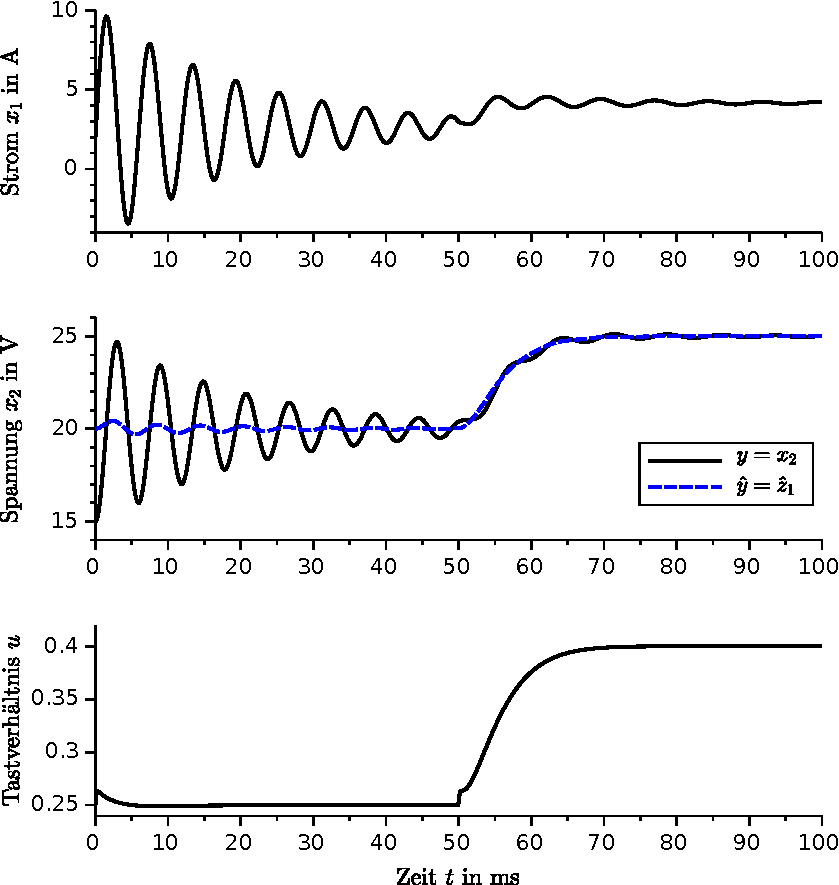
\includegraphics[width=0.8\textwidth]{Hochsetzsteller_IMC_Spannung}
\par\end{centering}
\caption{Simulation des Hochsetzstellers mit dem IMC-Regler aus Beispiel~\ref{exa:Hochsetzsteller-IMC-Spannung}\ref{exa:hochsetzsteller-IMC}\label{fig:Hochsetzsteller-IMC-Spannung}}
\end{figure}


\section{Approximative Linearisierung durch Modifikation\label{sec:Approximative-Linearisierung-Modifikation}}

Bei den bisherigen Betrachtung wurde für das System~(\ref{eq:var-basissystem})
immer ein wohldefinierter relativer Grad vorausgesetzt. Andernfalls
ist die in Kapitel~\ref{chap:regler-grundlagen} beschriebene exakte
Linearisierung nicht (direkt) anwendbar. Mit dem in~\cite{hauser92}
vorgestellten Zugang wird bei nicht wohldefiniertem relativen Grad
eine approximative Linearisierung erzielt\index{Linearisierung!approximative}.

Der relative Grad von System~(\ref{eq:var-basissystem}) ist im Punkt
$p\in\mathcal{M}$ \textit{nicht} wohldefiniert, wenn die erste nicht
verschwindende Lie-Ableitung im Punkt~$p$ Null ist, d.\,h. 
\[
L_{g}L_{f}^{r-1}h(x)\not\equiv0,\quad\text{aber}\quad L_{g}L_{f}^{r-1}h(p)=0.
\]
Das bedeutet, dass beim ersten Auftreten des Eingangs in den Zeitableitungen
des Ausgangs 
\[
\begin{array}{lcl}
y & = & h(x)\\
 & \vdots\\
y^{(r-1)} & = & L_{f}^{r-1}h(x)\\
y^{(r)} & = & L_{f}^{r}h(x)+L_{g}L_{f}^{r-1}h(x)\,u
\end{array}
\]
der Faktor $L_{g}L_{f}^{r-1}h(x)$ vor dem Eingang~$u$ im Punkt~$p$
verschwindet. Aus Stetigkeitsgründen ist dann $L_{g}L_{f}^{r-1}h(x)$
für alle~$x$ aus einer (hinreichend kleinen) Umgebung von~$p$
auch betragsmäßig klein. Der in~\cite{hauser92} vorgestellte Ansatz
beruht darauf, dass man den Term $L_{g}L_{f}^{r-1}h(x)u$ vernachlässigt
und weiter differenziert. Diese Ableitungsbildung unter Vernachlässigung
des angegebenen Terms lässt sich über Lie-Ableitungen entlang des
Vektorfelds~$f$ darstellen. Unter dem sich dabei ergebenden Diffeomorphismus
$\xi=\Phi(x)$ mit $\xi_{1}=h(x),\,\xi_{2}=L_{f}h(x),\ldots,\xi_{n}=L_{f}^{n-1}h(x)$
erhält man das transformierte System
\begin{equation}
\begin{array}{lcl}
\dot{\xi}_{1} & = & \xi_{2}\\
 & \vdots\\
\dot{\xi}_{r-1} & = & \xi_{r}\\
\dot{\xi}_{r} & = & \xi_{r+1}+\beta_{r}(\xi)\,u\\
 & \vdots\\
\dot{\xi}_{n-1} & = & \xi_{n}+\beta_{n-1}(\xi)\,u\\
\dot{\xi}_{n} & = & \alpha_{n}(\xi)+\beta_{n}(\xi)\,u
\end{array}\label{eq:var-approx-ARNF}
\end{equation}
mit 
\[
\alpha_{n}(\xi)=L_{f}^{n}h(\Phi^{-1}(\xi)),\quad\beta_{i}(\xi)=L_{g}L_{f}^{i-1}h(\Phi^{-1}(\xi)),\quad i=r,\ldots,n.
\]

Für die approximative Linearisierung\index{Linearisierung!approximative}
nehmen wir an, dass die Terme $\beta_{r},\ldots\beta_{n-1}$ im betreffenden
Arbeitsbereich (betragsmäßig) kleine Werte annehmen, der Term~$\beta_{n}$
sich aber erheblich von der Null unterscheidet. Die Linearisierung
durch Rückführung führt man in der letzten Zeile von System~(\ref{eq:var-approx-ARNF})
mit dem fiktiven Eingang~$v$ durch:
\begin{equation}
v\stackrel{!}{=}\alpha_{n}(\xi)+\beta_{n}(\xi)\,u\quad\Longleftrightarrow\quad u=\frac{1}{\beta_{n}(\xi)}\left(v-\alpha_{n}(\xi)\right).\label{eq:var-approximativ-linearisierende-rueckfuehrung}
\end{equation}
Zur Stabilisierung kombiniert man die (approximativ) linearisierende
Rückführung~(\ref{eq:var-approximativ-linearisierende-rueckfuehrung})
mit der Rückführung $v=-k^{T}\xi$. Die Verstärkung $k^{T}=(a_{0},\ldots,a_{n})$
enthält die Koeffizienten eines vorgegebenen charakteristischen Polynoms
\begin{equation}
\det\left(sI-\left(A-bk^{T}\right)\right)=a_{0}+a_{1}s+\cdots+a_{n-1}s^{n-1}+s^{n}.\label{eq:var-al-char-poly}
\end{equation}
Somit erhält man für die Originalkoordinaten in Anlehnung an Abschnitt~\ref{sec:E-A-Linearisierung-affin}
das Regelgesetz
\begin{equation}
u=-\frac{1}{L_{g}L_{f}^{n-1}h(x)}\sum_{i=0}^{n}a_{i}L_{f}^{i}h(x)\quad\text{mit}\quad a_{n}:=1.\label{eq:var-approx-rueckfuehrung-x}
\end{equation}
In ähnlicher Weise lassen sich auch die in den Abschnitten~\ref{sec:Trajektorienfolgeregelung-Feedback}
und~\ref{sec:Trajektorienfolgeregelung-Feedforward} beschriebenen
Rückführungen für Trajektorienfolgeregelungen nutzen. Die Stabilisierung
des rückgeführten Systems kann man mit Überlegungen des High-Gain-Entwurfs
begründen (vgl. Kapitel~\ref{chap:High-Gain-Beobachter}). 

\medskip{}

Die approximative Linearisierung wird in~\cite{hauser92,sastry1999}
am Beispiel eines Balls auf einem Balken (engl. ball \& beam example)
untersucht. Dieses Beispiel wurde in etlichen weiteren Veröffentlichungen
aufgegriffen~\cite{leith2001,zhang2006feedback}. In~\cite{zimmer1995,sastry1998helicopter}
wird die approximtive Linearisierung eines Hubschraubermodells behandelt.
Das folgende Beispiel ist an~\cite{aguilar2002approximate} angelehnt:
\begin{example}
\label{exa:wagen-pendel-approximativ}Wir betrachten das partiell
linearisierte Modell des Wagen-Pendel-Systems aus Abschnitt~\ref{subsec:Wagen-mit-Pendel}
und Beispiel~\ref{exa:Wagen-Pendel-partielle-Linearisierung} unter
Vernachlässigung der Reibung:
\begin{equation}
\begin{array}{lcl}
\dot{x}_{1} & = & x_{2}\\
\dot{x}_{2} & = & v\\
\dot{x}_{3} & = & x_{4}\\
\dot{x}_{4} & = & -\frac{g}{l}\sin x_{3}-\frac{1}{l}v\cos x_{3}\\
y & = & x_{1}.
\end{array}\label{eq:var-approx-wagen-pendel-linearisiert}
\end{equation}
In Beispiel~\ref{exa:Wagen-Pendel-max-rel-grad} wurde für dieses
System der (fiktive) Ausgang
\begin{equation}
h(x)=x_{1}+\frac{l}{2}\ln\left(\frac{1+\sin x_{3}}{1-\sin x_{3}}\right)\label{eq:var-approx-wagen-ausgang-r-3}
\end{equation}
ermittelt, mit dem das System wegen $L_{g}h(x)=L_{g}L_{f}h(x)=0$
und $L_{g}L_{f}^{2}h(x)=-2x_{4}\tan x_{3}$ für $x_{3}\neq k\pi$,
$k\in\Z$ und $x_{4}\neq0$ den (maximalen) relativen Grad $r=3$
besitzt. Im Punkt $x=0$ ist der relative Grad damit nicht definiert.
Für die Approximation gehen wir von $x_{3}\approx0$ (kleine Auslenkung
des Pendels) und $x_{4}\approx0$ (kleine Winkelgeschindigkeit) aus
und bestimmen die gemischte Lie-Ableitung der nächsthöheren Ordnung:
\begin{equation}
L_{g}L_{f}^{3}h(x)=\frac{\left(3l\cos\left(2x_{3}\right)-9l\right)x_{4}^{2}+\left(\cos\left(3x_{3}\right)-3\cos x_{3}\right)g}{l\left(\cos\left(2x_{3}\right)+1\right)}.\label{eq:var-approx-wagen-gemischte-Lie-Ableitung}
\end{equation}
Mit $L_{g}L_{f}^{3}h(0)=-g/l$ ist dieser Term im Arbeitspunkt $x=0$
nicht vernachlässigbar. Für die Rückführung~(\ref{eq:var-approx-rueckfuehrung-x})
benötigt man neben~(\ref{eq:var-approx-wagen-gemischte-Lie-Ableitung})
und dem Ausgang~(\ref{eq:var-approx-wagen-ausgang-r-3}) noch die
Lie-Ableitungen
\[
\begin{array}{lcl}
L_{f}h(x) & = & x_{2}+\frac{lx_{4}}{\cos x_{3}}\\
L_{f}^{2}h(x) & = & \tan x_{3}\left(g+\frac{lx_{4}^{2}}{\cos x_{3}}\right)\\
L_{f}^{3}h(x) & = & 2gx_{4}\,\frac{1-\cos(2x_{3})}{1+\cos(2x_{3})}+lx_{4}^{3}\,\frac{1-\sin^{4}x_{3}}{\cos^{5}x_{3}}\\
L_{f}^{4}h(x) & = & 2lx_{4}^{4}\frac{\sin x_{3}}{\cos^{2}x_{3}}\left(\frac{6}{\cos^{2}x_{3}}-1\right)+3gx_{4}^{2}\sin x_{3}\left(\frac{4}{\cos^{2}x_{3}}-1\right)\\
 &  & +\,\frac{g^{2}}{l}\sin x_{3}\left(\frac{3}{\cos^{2}x_{3}}-2\right).
\end{array}
\]

Zur numerischen Simulation verwenden wir mit Ausnahme von $d_{1}=0$
und $d_{2}=0$ (Vernachlässigung der Reibung) die Parameter und Anfangswerte
aus Beispiel~\ref{exa:Wagen-Pendel-Stabilisierung-Simulation}. Die
Eigenwerte werden durch $s_{1,2}=-2$ und $s_{3,4}=-3$ vorgegeben.
Das Simulationsergebnis ist Abb.~\ref{fig:Simulation-Wagen-Pendel-Approx-Lin}
zu entnehmen. Im Unterschied zur Regelung mittels Eingangs-Ausgangs-Linearisierung
in Beispiel~\ref{exa:Wagen-Pendel-Stabilisierung-Simulation} wird
jetzt die Dynamik für alle Zustände eingeprägt. Im Vergleich zu Abb.~\ref{fig:Simulation-Wagen-Pendel-System}
erfolgt hier ein schnelleres Einschwingen.
\end{example}
\begin{figure}
\begin{centering}
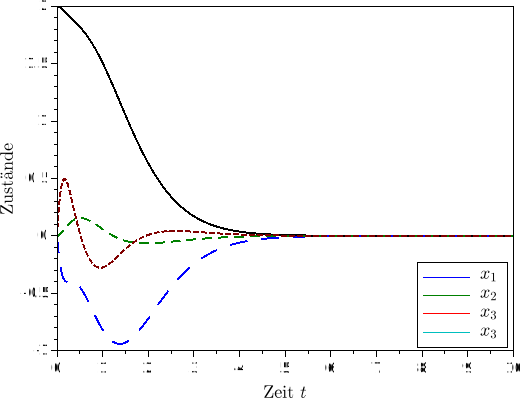
\includegraphics[width=0.85\textwidth]{Wagen_Pendel_Approx}
\par\end{centering}
\caption{Simulationsergebnis des geregelten Wagen-Pendel-Systems\label{fig:Simulation-Wagen-Pendel-Approx-Lin}}
\end{figure}

\begin{remark}
Den Reglerentwurf führt man nach Gl.~(\ref{eq:var-approx-rueckfuehrung-x})
so durch, als ob die Terme $\beta_{r},\ldots,\beta_{n-1}$ in Gl.~(\ref{eq:var-approx-ARNF})
identisch Null wären. Diese Annahme kann man auch als Modifikation
des Systems interpretieren, wodurch das resultierende System eingangs-zustands-linearisierbar
wird. Das Nullsetzen von $\beta_{r},\ldots,\beta_{n-1}$ in Gl.~(\ref{eq:var-approx-ARNF})
führt in Originalkoordinaten auf das modifizierte Vektorfeld 
\[
\tilde{g}(x)=\left[\Phi^{\prime}(x)\right]^{-1}\cdot\left.\beta_{n}(z)\frac{\partial}{\partial z_{n}}\right|_{z=\Phi(x)}=L_{g}L_{f}^{n-1}h(x)\cdot\left[\Phi^{\prime}(x)\right]^{-1}\cdot e_{n}.
\]
In ähnlicher Weise kann man auch durch Modifikation des Vektorfeldes~$f$
ein eingangs-zustands-linearisierbares System erzeugen~\cite{hauser92}.
\end{remark}

\section{Approximative Linearisierung durch Reihenentwicklung\label{sec:Approximative-Linearisierung-Reihenentwicklung}}

Um die einschränkenden Existenzbedingungen bzw. die schwierige Berechnung
für eine exakte Eingangs-Zustands-Linearisierung zu umgehen, wurden
in der Fachliteratur zahlreiche Approximationsansätze\index{Linearisierung!approximative}
vorgeschlagen~\cite{reboulet84,baumann86,guardabassi2001}. Etliche
Veröffentlichungen basieren auf einer Transformation des betreffenden
Systems in die Poincaré-Normalform\index{Normalform!Poincaré-}~\cite{krener84,krener90,krener91poincare,devanathan2001,devanathan2004}.
Dabei setzt man sowohl für das System als auch für die Transformation~$\Phi$
eine mehrvariable Taylor\-reihe an und versucht, die von den Nichtlinearitäten
herrührenden Terme höherer Ordnung schrittweise zu eliminieren. Da
die Anzahl der Terme einer mehrvariablen Taylorentwicklung exponentiell
mit der Entwicklungsordnung wächst, ist dieser Ansatz nur bedingt
praktikabel. 

Der in diesem Abschnitt vorgestellte Zugang nach~\cite{roebenack2012pamm,roebenack2013ecc,franke2015buch}
vermeidet die Reihenentwicklung der Koordinatentransformation und
kann in gewisser Weise als das Gegenstück zum erweiterten Luenberger-Beobachter
aufgefasst werden (vgl. Abschnitt~\ref{subsec:Luenberger}).

\subsection{Vorüberlegungen und exakte Linearisierung\label{subsec:Approx-exakt}}

Man betrachte eine eingangsaffine Regelstrecke 
\begin{equation}
\dot{x}=f(x)+g(x)\,u\label{eq:var-basissystem-ohne-ausgang}
\end{equation}
mit hinreichend glatten Vektorfeldern $f,g:\mathcal{M}\to\R^{n}$
auf einer offenen Menge $\mathcal{M}\subseteq\R^{n}$. Das System
ist in einem Punkt $p\in\mathcal{M}$ exakt eingangs-zustands-linearisierbar,
wenn es eine Ausgangsabbildung $h:\mathcal{M}\to\R$ gibt, für die
das System den relativen Grad~$n$ besitzt, also
\begin{equation}
L_{g}h(x)=0,\;L_{g}L_{f}h(x)=0,\;\ldots,\;L_{g}L_{f}^{n-2}h(x)=0,\;L_{g}L_{f}^{n-1}h(p)\neq0\label{eq:var-al-rel-grad-n-allgemein}
\end{equation}
für alle~$x$ aus einer Umgebung von~$p$ gilt (vgl. Abschnitt~\ref{sec:Exakte-Eingangs-Zustands-Linearisierung}).
Wir gehen im Folgenden von der etwas strengeren Bedingung
\begin{equation}
L_{g}h(x)=0,\;L_{g}L_{f}h(x)=0,\;\ldots,\;L_{g}L_{f}^{n-2}h(x)=0,\;L_{g}L_{f}^{n-1}h(x)=1\label{eq:var-al-rel-grad-n-speziell}
\end{equation}
für alle~$x$ aus einer Umgebung von~$p$ aus.\footnote{Gilt~(\ref{eq:var-al-rel-grad-n-allgemein}), dann kann die Bedingung~(\ref{eq:var-al-rel-grad-n-speziell})
immer durch eine zustandsäbhängige Eingangstransformation $u\mapsto\tfrac{1}{L_{g}L_{f}^{n-1}h(x)}u$
erzwungen werden (vgl. Abschnitt~\ref{subsec:EZ-Linearisierung-Formen}).} Die Ausgangsabbildung~$h$ ist die Lösung der (partiellen) Differentialgleichung
\begin{equation}
\d h(x)=\omega(x),\label{eq:var-al-dh-omega}
\end{equation}
wobei sich das Kovektorfeld~$\omega$ aus der Steuerbarkeitsmatrix\index{Steuerbarkeitsmatrix}\index{Matrix!Steuerbarkeits-}
\begin{equation}
Q_{S}(x)=\left(g(x),\ad_{-f}g(x),\ldots,\ad_{-f}^{n-1}g(x)\right)\label{eq:var-al-steuerbarkeitsmatrix}
\end{equation}
entsprechend
\begin{equation}
\omega(x)=e_{n}^{T}Q_{S}^{-1}(x)\label{eq:var-al-startkovektor}
\end{equation}
mit dem $n$-ten Einheitsvektor~$e_{n}$ ergibt. Kennt man die Abbildung~$h$,
dann lässt sich das System mit dem Diffeomorphismus 
\begin{equation}
\xi=\Phi(x)=\left(\begin{array}{c}
h(x)\\
L_{f}h(x)\\
\vdots\\
L_{f}^{n-1}h(x)
\end{array}\right),\quad x=\Psi(\xi):=\Phi^{-1}(\xi)\label{eq:var-al-transformation}
\end{equation}
in die spezielle Variante
\begin{equation}
\left.\begin{array}{lcl}
\dot{\xi}_{1} & = & \xi_{2}\\
 & \vdots\\
\dot{\xi}_{n-1} & = & \xi_{n}\\
\dot{\xi}_{n} & = & \alpha(\xi)+u\\
y & = & \xi_{1}
\end{array}\right\} \quad\begin{array}{rcl}
\dot{\xi} & = & A\xi+b(\alpha(\xi)+u)\\
y & = & c^{T}\xi
\end{array}\label{eq:var-Regelungs-NF-speziell}
\end{equation}
der Regelungsnormalform transformieren (vgl. Abschnitt~\ref{subsec:EZ-Linearisierung-Formen}). 

In diesem Abschnitt erfolgt der Reglerentwurf ohne explizite Kenntnis
der zur exakten Eingangs-Zustands-Linearisierung benötigten Ausgangsabbildung~$h$.
Das bedeutet, dass zwar die Flachheit des Systems~(\ref{eq:var-basissystem-ohne-ausgang})
vorausgesetzt wird (vgl. Abschnitt~\ref{subsec:Flacher-nichtflacher-Ausgang}),
der flache Ausgang aber nicht unmittelbar für die Regelung benötigt
wird.

Die gewünschte Dynamik von System~(\ref{eq:var-basissystem-ohne-ausgang})
sei durch Referenztrajektorien $u_{\text{ref}}(\cdot)$ und $x_{\text{ref}}(\cdot)$
gegeben, d.\,h. diese Referenztrajektorien genügen der Systemgleichung
\begin{equation}
\dot{x}_{\text{ref}}=f(x_{\text{ref}})+g(x_{\text{ref}})\,u_{\text{ref}}.\label{eq:var-al-referenz-system}
\end{equation}
Die Berechnung dieser Trajektorien ist rein numerisch über die Lösung
einer entsprechenden Randwertaufgabe möglich (vgl. Abschnitt~\ref{subsec:Berechnung-Referenztraj-randwert}).
Ähnlich wie in den Abschnitten~\ref{sec:Trajektorienfolgeregelung-Feedback}
und~\ref{sec:Trajektorienfolgeregelung-Feedforward} teilen wir das
Eingangssignal 
\[
u=u_{\text{ref}}+u_{\text{stab}}
\]
in jeweils einen Anteil zur Vorsteuerung und zur Stabilisierung auf.
Die Vorsteuerung erfolgt über die Referenztrajektorie~$u_{\text{ref}}$.
Die Referenztrajektorie~$x_{\text{ref}}$ soll über eine Rückführung
$\kappa:\mathcal{M}\to\R$ mit
\begin{equation}
u_{\text{stab}}=u-u_{\text{ref}}=-\kappa(x)\label{eq:var-al-stab}
\end{equation}
stabilisiert werden. Der geschlossene Regelkreis nimmt dadurch die
Form
\[
\dot{x}=f(x)+g(x)\left(u_{\text{ref}}-\kappa(x)\right)
\]
an.

Der eigentliche Reglerentwurf erfolgt zunächst in der Normalform~(\ref{eq:var-Regelungs-NF-speziell}).
Mit dem Ansatz~(\ref{eq:var-al-stab}) erhält man 
\[
\begin{array}{lcl}
\dot{\xi} & = & A\xi+b(\alpha(\xi)+u)\\
 & = & A\xi+b(\alpha(\xi)+u_{\text{ref}}-\kappa(\Psi(\xi))
\end{array}
\]
für die Regelstrecke~(\ref{eq:var-Regelungs-NF-speziell}). Das transformierte
Referenzsystem~(\ref{eq:var-al-referenz-system}) nimmt die Gestalt
\[
\dot{\xi}_{\text{ref}}=A\xi_{\text{ref}}+b\left(\alpha(\xi_{\text{ref}})+u_{\text{ref}}\right)
\]
an. Der Folgefehler $\tilde{\xi}=\xi-\xi_{\text{ref}}$ genügt damit
der Differentialgleichung
\begin{equation}
\begin{array}{lcl}
\dot{\tilde{\xi}} & = & \dot{\xi}-\dot{\xi}_{\text{ref}}\\
 & = & A\tilde{\xi}+b(\alpha(\xi)-\alpha(\xi_{\text{ref}})-\kappa(\Psi(\xi)).
\end{array}\label{eq:var-al-fehlerdyn1}
\end{equation}
Mit der Rückführung 
\begin{equation}
\kappa(x)=\kappa(\Phi^{-1}(\xi))=\alpha(\xi)-\alpha(\xi_{\text{ref}})+k^{T}\tilde{\xi},\quad k\in\R^{n}\label{eq:var-al-regler-exakt-xi}
\end{equation}
erhält man eine exakt lineare Fehlerdynamik
\begin{equation}
\dot{\tilde{\xi}}=\left(A-bk^{T}\right)\tilde{\xi}.\label{eq:var-al-fehlerdynamik-linear}
\end{equation}
Setzt man dabei die Reglerverstärkung~$k$ in der Form $k^{T}=\left(a_{0},\ldots,a_{n-1}\right)$
an, so ergibt sich (bedingt durch die Brunovský-Form des Paares $(A,b)$)
das charakteristische Polynom~(\ref{eq:var-al-char-poly}). In Originalkoordinaten
nimmt das Regelgesetz~(\ref{eq:var-al-regler-exakt-xi}) die Form
\begin{equation}
\kappa(x)=\sum_{i=0}^{n}a_{i}L_{f}^{i}h(x)-\sum_{i=0}^{n}a_{i}\underbrace{L_{f}^{i}h(x_{\text{ref}}(t))}_{{\displaystyle y_{\text{ref}}^{(i)}}(t)}\label{eq:var-al-regler-exakt}
\end{equation}
mit der Ausgangsreferenztrajektorie $y_{\text{ref}}(\cdot)=h(x_{\text{ref}}(\cdot))$
und $a_{n}:=1$ an.\footnote{Bedingt durch die Abhängigkeit von der Referenztrajektorie ist die
Rückführung~$\kappa$ auch von der Zeit~$t$ abhängig. Aus Gründen
der Übersichtlichkeit wurde auf die explizite Angabe dieser Abhängigkeit
verzichtet.} Dieses Regelgesetz ist eine spezielle Variante der in Abschnitt~\ref{sec:Trajektorienfolgeregelung-Feedback}
vorgestellten Rückführung~(\ref{eq:folgeregelung-feedback}).

\begin{example}
\label{exa:Inverses-Pendel-Approx-Exakt}Das in Beispiel~\ref{exa:inverses-pendel-gleichstrommotor}
modellierte inverse Pendel mit Gleich\-strom\-antrieb lässt sich
durch ein System~(\ref{eq:var-basissystem-ohne-ausgang}) mit den
Vektorfeldern
\begin{equation}
f(x)=\left(\begin{array}{c}
x_{2}\\
\frac{mg\ell}{J}\sin x_{1}-\frac{d}{J}x_{2}+\frac{K}{J}x_{3}\\
-\frac{K}{L}x_{2}-\frac{R}{L}x_{3}
\end{array}\right),\quad g(x)=\left(\begin{array}{c}
0\\
0\\
\frac{1}{L}
\end{array}\right)\label{eq:var-al-inv-pend-system}
\end{equation}
beschreiben. Im Zusammenhang mit einer exakten Eingangs-Zustands-Linearisierung
wurde in Beispiel~\ref{exa:inverses-pendel-gleichstrommotor-formen}
entsprechend Gl.~(\ref{eq:var-al-startkovektor}) das Kovektorfeld
\begin{equation}
\omega(x)=\left(\unit{\tfrac{JL}{K}},0,0\right)=\tfrac{JL}{K}\,\d x_{1}\label{eq:var-al-inv-pend-omega}
\end{equation}
ermittelt. Durch Integration erhält man daraus die Ausgangsabbildung
$h(x)=\tfrac{JL}{K}x_{1},$ mit der das System~(\ref{eq:var-al-inv-pend-system})
die Bedingung~(\ref{eq:var-al-rel-grad-n-speziell}) erfüllt und
daher zustandsäquivalent zu der speziellen Regelungsnormalform~(\ref{eq:var-Regelungs-NF-speziell})
ist. Das Regelgesetz~(\ref{eq:var-al-regler-exakt}) lässt sich unmittelbar
über die Lie-Ableitungen des Skalarfeldes~$h$ entlang des Vektorfeldes~$f$
berechnen.
\end{example}

\subsection{Approximation nullter Ordnung\label{subsec:Approx-nullter-Ordnung}}

Das exakt linearisierende Regelgesetz~(\ref{eq:var-al-regler-exakt})
setzt die Kenntnis der Ausgangsabbildung~$h$ voraus. Die nachfolgenden
Überlegungen führen auf ein Regelgesetz, für dessen Berechnung die
nur als Hilfsgröße eingeführte Ausgangsabbildung~$h$ nicht unmittelbar
benötigt wird.

Wir betrachten die Reihenentwicklung 
\begin{equation}
\begin{array}{lcl}
\kappa(\Psi(\xi)) & = & \left.\frac{\partial\kappa}{\partial x}\frac{\partial x}{\partial\xi}\right|_{\xi_{\text{ref}}}\cdot(\xi-\xi_{\text{ref}})+\mathcal{O}\left(\|\tilde{\xi}\|^{2}\right)\\
 & = & \d\kappa(x_{\text{ref}})\cdot\Psi^{\prime}(\xi_{\text{ref}})\cdot\tilde{\xi}+\mathcal{O}\left(\|\tilde{\xi}\|^{2}\right)
\end{array}\label{eq:var-al-reihe1}
\end{equation}
des gesuchten Regelgesetzes $\kappa(\Psi(\xi))$ entlang der Referenztrajektorie~$\xi_{\text{ref}}$.
Bei dieser Reihenentwicklung entfällt das Absolutglied, da dessen
Anteil schon in der Steuerung~$u_{\text{ref}}$ Berücksichtigung
findet. Setzt man die Reihenentwicklung~(\ref{eq:var-al-reihe1})
in die Fehlerdynamik~(\ref{eq:var-al-fehlerdyn1}) ein, so erhält
man 
\begin{equation}
\dot{\tilde{\xi}}=\left(A-b\d\kappa(x_{\text{ref}})\Psi^{\prime}(\xi_{\text{ref}})\right)\tilde{\xi}+b(\alpha(\xi)-\alpha(\xi_{\text{ref}}))+\mathcal{O}\left(\|\tilde{\xi}\|^{2}\right).\label{eq:var-al-fehlerdyn2}
\end{equation}
Den Gradienten $\d\kappa$ ersetzen wir durch ein allgemeines Kovektorfeld
\begin{equation}
\sigma(x_{\text{ref}})=\d\kappa(x_{\text{ref}}).\label{eq:var-al-verstaerkung-als-gradient}
\end{equation}
Mit der Wahl 
\begin{equation}
\sigma(x_{\text{ref}})=k^{T}\cdot\left(\Psi^{\prime}(\xi_{\text{ref}})\right)^{-1}\label{eq:var-al-verstaerkung-z}
\end{equation}
geht die Fehlerdynamik~(\ref{eq:var-al-fehlerdyn2}) in die Differentialgleichung
\begin{equation}
\dot{\tilde{\xi}}=\left(A-bk^{T}\right)\tilde{\xi}+b(\alpha(\xi)-\alpha(\xi_{\text{ref}}))+\mathcal{O}\left(\|\tilde{\xi}\|^{2}\right)\label{eq:var-al-fehlerdyn-ordnung-0}
\end{equation}
über. In der Reihenentwicklung von~(\ref{eq:var-al-fehlerdyn-ordnung-0})
liefert die Differenz $\alpha(\xi)-\alpha(\xi_{\text{ref}})$ den
Beitrag $\d\alpha(\xi_{\text{ref}})$ zu den Termen erster Ordnung.
Dieser Anteil wird nicht exakt kompensiert, sondern soll vom linearen
Teil $A-bk^{T}$ dominiert werden. Daher ist die Fehlerdynamik~(\ref{eq:var-al-fehlerdyn-ordnung-0})
nur als Approximation nullter Ordnung einer exakt linearen Fehlerdifferentialgleichung~(\ref{eq:var-al-fehlerdynamik-linear})
aufzufassen.

Das aus der Steuerbarkeitsmatrix~(\ref{eq:var-al-steuerbarkeitsmatrix})
nach Gl.~(\ref{eq:var-al-startkovektor}) berechnete Kovektorfeld~$\omega$
erfüllt unter der Annahme~(\ref{eq:var-al-rel-grad-n-speziell})
die Bedingung~(\ref{eq:var-al-dh-omega}). Das bedeutet, dass $\omega$
ein exaktes Differential ist. Nach Proposition~\ref{prop:Kovektorfelder}
gilt somit $\d L_{f}h(x)=L_{f}\d h(x)=L_{f}\omega(x)$. Daher lässt
sich die Jacobimatrix der Transformation~(\ref{eq:var-al-transformation})
ohne explizite Kenntnis des Ausgangs~$h$ darstellen:
\[
\left(\Psi^{\prime}(\xi)\right)^{-1}=\Phi^{\prime}(x)=\frac{\partial}{\partial x}\left(\begin{array}{c}
h(x)\\
L_{f}h(x)\\
\vdots\\
L_{f}^{n-1}h(x)
\end{array}\right)\!=\!\left(\begin{array}{c}
\d h(x)\\
\d L_{f}h(x)\\
\vdots\\
\d L_{f}^{n-1}h(x)
\end{array}\right)\!=\!\left(\begin{array}{c}
\omega(x)\\
L_{f}\omega(x)\\
\vdots\\
L_{f}^{n-1}\omega(x)
\end{array}\right).
\]
Die vom Referenzzustand~$x_{\text{ref}}$ abhängige Verstärkung~(\ref{eq:var-al-verstaerkung-z})
kann dann in Originalkoordinaten 
\begin{equation}
\sigma(x_{\text{ref}})=a_{0}\omega(x_{\text{ref}})+a_{1}L_{f}\omega(x_{\text{ref}})+\cdots+a_{n-1}L_{f}^{n-1}\omega(x_{\text{ref}})\label{eq:var-al-verstaerkung-x}
\end{equation}
unter Verwendung der Koeffizienten des charakteristischen Polynoms~(\ref{eq:var-al-char-poly})
angegeben werden. Die Rückführung~(\ref{eq:var-al-stab}) nimmt unter
Beachtung von~(\ref{eq:var-al-reihe1}) und~(\ref{eq:var-al-verstaerkung-als-gradient})
die Form 
\[
\kappa(x)=\sigma(x_{\text{ref}})\,(x-x_{\text{ref}})=\sigma(x_{\text{ref}})\,\tilde{x}
\]
an.

\begin{example}
\label{exa:Inverses-Pendel-Approx-0}Für das System~(\ref{eq:var-al-inv-pend-system})
aus Beispiel~\ref{exa:Inverses-Pendel-Approx-Exakt} erhält man das
in Gl.~(\ref{eq:var-al-inv-pend-omega}) angegebene Kovektorfeld~$\omega$.
Daraus berechnet man nach Gl.~(\ref{eq:var-al-verstaerkung-x}) mit
\textsc{Maxima} unter Zuhilfenahme der in Alg.~\ref{alg:Lie-Ableitung-Kovektor}
beschriebenen Routine \texttt{LieCovector} die folgende Reglerverstärkung:

\begin{maxima}\noindent
%%%%%%%%%%%%%%%
%%% INPUT:
\begin{minipage}[t]{8ex}\color{red}\bf
\begin{verbatim}
(%i5) 
\end{verbatim}
\end{minipage}
\begin{minipage}[t]{\textwidth}\color{blue}
\begin{verbatim}
f:[x2,(m*G*l*sin(x1)-d*x2+K*x3)/J,-(K*x2+R*x3)/L]$
ω:[J*L/K,0,0]$
x:[x1,x2,x3]$
n:length(x)$
\end{verbatim}
\end{minipage}

\smallskip

\noindent
%%%%%%%%%%%%%%%
%%% INPUT:
\begin{minipage}[t]{8ex}\color{red}\bf
\begin{verbatim}
(%i6) 
\end{verbatim}
\end{minipage}
\begin{minipage}[t]{\textwidth}\color{blue}
\begin{verbatim}
σ:sum(a[i]*LieCovector(f,ω,x,i),i,0,n-1);
\end{verbatim}
\end{minipage}
%%% OUTPUT:

\noindent
$\displaystyle
\parbox{8ex}{$\color{labelcolor}\mathrm{\tt (\%o6) }\quad $}
[\frac{{{a}_{0}}\cdot J\cdot L}{K}+\frac{{{a}_{2}}\cdot l\cdot m\cdot \mathrm{cos}\left( \mathit{x1}\right) \cdot G\cdot L}{K},\frac{{{a}_{1}}\cdot J\cdot L}{K}-\frac{{{a}_{2}}\cdot d\cdot L}{K},{{a}_{2}}\cdot L]\mbox{}
$
%%%%%%%%%%%%%%%
\end{maxima}
\end{example}

\subsection{Approximation erster Ordnung\label{subsec:Approx-erster-Ordnung}}

Das im letzten Abschnitt hergeleitete Regelgesetz~(\ref{eq:var-al-verstaerkung-x})
soll dahingehend verbessert werden, dass man eine näherlungsweise
lineare Fehlerdynamik und damit eine Approximation erster Ordnung
erhält. Dazu führen wir eine Reihenentwicklung der Nichtlinearität~$\alpha$
entlang der Referenztrajektorie durch
\[
\alpha(\xi)=\alpha(\xi_{\text{ref}})+\d\alpha(\xi_{\text{ref}})\,\tilde{\xi}+\mathcal{O}\left(\|\tilde{\xi}\|^{2}\right)
\]
und setzen diesen Ansatz in die Fehlerdifferentialgleichung~(\ref{eq:var-al-fehlerdyn2})
ein:
\[
\dot{\tilde{\xi}}=\left(A-b\left(\d\kappa(x_{\text{ref}})\Psi^{\prime}(\xi_{\text{ref}})-\d\alpha(\xi_{\text{ref}})\right)\right)\tilde{\xi}+\mathcal{O}\left(\|\tilde{\xi}\|^{2}\right).
\]
Um eine näherungsweise lineare Fehlerdynamik
\begin{equation}
\dot{\tilde{\xi}}=\left(A-bk^{T}\right)\tilde{\xi}+\mathcal{O}\left(\|\tilde{\xi}\|^{2}\right)\label{eq:var-al-fehlerdyn-ordnung-1}
\end{equation}
zu erzeugen, muss die Reglerverstärkung~(\ref{eq:var-al-verstaerkung-als-gradient})
entsprechend
\begin{equation}
\sigma(x_{\text{ref}})=k^{T}\left(\Psi^{\prime}(\xi_{\text{ref}})\right)^{-1}+\d\alpha(\xi_{\text{ref}})\left(\Psi^{\prime}(\xi_{\text{ref}})\right)^{-1}\label{eq:var-al-verstaerkung1-z}
\end{equation}
gewählt werden. Der erste Summand hat in Originalkoordinaten die Form~(\ref{eq:var-al-verstaerkung-x}).
Zur Bestimmung des zweiten Summanden betrachten wir die Nichtlinearität~$\alpha$
in Originalkoordinaten:
\[
\begin{array}{ccl}
\alpha(\xi) & = & L_{f}^{n}h(x)\\
 & = & \left\langle \d L_{f}^{n-1}h,f\right\rangle (x)\\
 & = & \left\langle L_{f}^{n-1}\d h,f\right\rangle (x)\\
 & = & \left\langle L_{f}^{n-1}\omega,f\right\rangle (x).
\end{array}
\]
Damit lässt sich der Gradient~$\d\alpha$ wie folgt darstellen:
\[
\begin{array}{ccl}
\d\alpha(\xi) & = & \frac{\partial\left\langle L_{f}^{n-1}\omega,f\right\rangle (x)}{\partial x}\cdot\frac{\d x}{\d\xi}\\
 & = & \frac{\partial\left\langle L_{f}^{n-1}\omega,f\right\rangle (x)}{\partial x}\cdot\Psi^{\prime}(\xi).
\end{array}
\]
Die Differentiation des Skalarprodukts liefert 
\[
\begin{array}{ccl}
\d\alpha(\xi)\left(\Psi^{\prime}(\xi)\right)^{-1} & = & \frac{\partial\left\langle L_{f}^{n-1}\omega,f\right\rangle (x)}{\partial x}\\
 & = & L_{f}^{n-1}\omega(x)f^{\prime}(x)+f^{T}(x)\frac{\partial\left(L_{f}^{n-1}\omega(x)\right)^{T}}{\partial x}\\
 & = & L_{f}^{n-1}\omega(x)f^{\prime}(x)+f^{T}(x)\left(\frac{\partial\left(L_{f}^{n-1}\omega(x)\right)^{T}}{\partial x}\right)^{T}\\
 & = & L_{f}^{n}\omega(x)
\end{array}
\]
unter Beachtung von Prop.~\ref{pro:Ableitungsregeln-Felder}. Dabei
wurde zusätzlich ausgenutzt, dass das Kovektorfeld~$\omega$ der
Gradient des Skalarfeldes~$h$ ist und die Ableitung von $L_{f}\omega$
somit eine Hessematrix darstellt (siehe Lemma~\ref{lem:Schwarz}).
Aus~(\ref{eq:var-al-verstaerkung1-z}) ergibt sich somit in Originalkoordinaten
die Reglerverstärkung 
\begin{equation}
\sigma(x_{\text{ref}})=a_{0}\omega(x_{\text{ref}})+a_{1}L_{f}\omega(x_{\text{ref}})+\cdots+a_{n-1}L_{f}^{n-1}\omega(x_{\text{ref}})+L_{f}^{n}\omega(x_{\text{ref}}).\label{eq:var-al-verstaerkung1-x}
\end{equation}

Die Reglerverstärkung~(\ref{eq:var-al-verstaerkung1-x}) kann man
als Verallgemeinerung der Ackermann-Formel~\cite{acker77,ackermann77}
für nichtlineare Systeme auffassen. Im Unterschied zur Ackermann-Formel
für lineare zeitvariante Systeme~\cite{freund71,foellinger78}, die
sich auf das entlang der Referenztrajektorie linearisierte System
anwenden lässt, kann der hier beschriebene Zugang unmittelbar auf
Approximationen höherer Ordnung erweitert werden.
\begin{example}
\label{exa:Inverses-Pendel-Approx-1}Wir betrachten wiederum das inverse
Pendel aus den Beispielen~\ref{exa:Inverses-Pendel-Approx-Exakt}
und~\ref{exa:Inverses-Pendel-Approx-0}. Zur Berechnung der Reglerverstärkung~(\ref{eq:var-al-verstaerkung1-x})
muss man das in Beispiel~\ref{exa:Inverses-Pendel-Approx-0} verwendete
\textsc{Maxima}-Skipt nur leicht modifizieren:

\begin{maxima}\noindent
%%%%%%%%%%%%%%%
%%% INPUT:
\begin{minipage}[t]{8ex}\color{red}\bf
\begin{verbatim}
(%i5) 
\end{verbatim}
\end{minipage}
\begin{minipage}[t]{\textwidth}\color{blue}
\begin{verbatim}
f:[x2,(m*G*l*sin(x1)-d*x2+K*x3)/J,-(K*x2+R*x3)/L]$
ω:[J*L/K,0,0]$
x:[x1,x2,x3]$
n:length(x)$
\end{verbatim}
\end{minipage}

\smallskip


\noindent
%%%%%%%%%%%%%%%
%%% INPUT:
\begin{minipage}[t]{8ex}\color{red}\bf
\begin{verbatim}
(%i7) 
\end{verbatim}
\end{minipage}
\begin{minipage}[t]{\textwidth}\color{blue}
\begin{verbatim}
sum(a[i]*LieCovector(f,ω,x,i),i,0,n)$
σ:subst([a[3]=1],%);
\end{verbatim}
\end{minipage}
%%% OUTPUT:

\noindent
$\displaystyle
\parbox{8ex}{$\color{labelcolor}\mathrm{\tt (\%o7) }\quad $}
[\frac{{{a}_{0}}\cdot J\cdot L}{K}-\frac{d\cdot l\cdot m\cdot \mathrm{cos}\left( \mathit{x1}\right) \cdot G\cdot L}{J\cdot K}-\frac{l\cdot m\cdot \mathrm{sin}\left( \mathit{x1}\right) \cdot \mathit{x2}\cdot G\cdot L}{K}+\frac{{{a}_{2}}\cdot l\cdot m\cdot \mathrm{cos}\left( \mathit{x1}\right) \cdot G\cdot L}{K},\frac{{{a}_{1}}\cdot J\cdot L}{K}+\frac{{{d}^{2}}\cdot L}{J\cdot K}+\frac{l\cdot m\cdot \mathrm{cos}\left( \mathit{x1}\right) \cdot G\cdot L}{K}-\frac{{{a}_{2}}\cdot d\cdot L}{K}-K,-R-\frac{d\cdot L}{J}+{{a}_{2}}\cdot L]\mbox{}
$
%%%%%%%%%%%%%%%
\end{maxima}
\end{example}

\subsection{Approximation zweiter Ordnung\label{subsec:Approx-zweiter-Ordnung}}

Die Approximation erster Ordnung wurde in Abschnitt~\ref{subsec:Approx-erster-Ordnung}
über die spezielle Variante~(\ref{eq:var-Regelungs-NF-speziell})
der Regelungsnormalform hergeleitet. In ähnlicher Weise lässt sich
auch eine Approximation zweiter Ordnung erzielen. Allerdings ist auf
diesem Weg die Berechnung der Reglerverstärkung vergleichsweise aufwendig~\cite{paschke2011da}.
Daher wird nachfolgend ein alternativer Ansatz vorgestellt, bei dem
man das exakt linearisierende Regelgesetz~(\ref{eq:var-al-regler-exakt})
in den Originalkoordinaten entlang der Referenztrajektorie~$x_{\text{ref}}$
in eine Reihe entwickelt~\cite{franke2015buch}.

Zunächst betrachten wir von der Lie-Ableitung $L_{f}h^{k}(x)$ entlang~$x_{\text{ref}}$
eine Reihenentwicklung erster Ordnung
\begin{equation}
\begin{array}{ccl}
L_{f}^{k}h(x) & = & L_{f}^{k}h(x_{\text{ref}})+\d L_{f}^{k}h(x_{\text{ref}})\,\tilde{x}+\mathcal{O}\left(\|\tilde{x}\|^{2}\right)\\
 & = & L_{f}^{k}h(x_{\text{ref}})+L_{f}^{k}\d h(x_{\text{ref}})\,\tilde{x}+\mathcal{O}\left(\|\tilde{x}\|^{2}\right)\\
 & = & L_{f}^{k}h(x_{\text{ref}})+L_{f}^{k}\omega(x_{\text{ref}})\,\tilde{x}+\mathcal{O}\left(\|\tilde{x}\|^{2}\right).
\end{array}\label{eq:var-al-reihe-lfh1}
\end{equation}
Setzt man diese Reihenentwicklung in das exakt linearisierende Regelgesetz~(\ref{eq:var-al-regler-exakt})
ein, so erhält man
\[
\kappa(x)=\sum_{i=0}^{n}a_{i}L_{f}^{i}\omega(x_{\text{ref}})\,\tilde{x}+\mathcal{O}\left(\|\tilde{x}\|^{2}\right)={\displaystyle \sigma(x_{\text{ref}})}\,\tilde{x}+\mathcal{O}\left(\|\tilde{x}\|^{2}\right)
\]
mit $a_{n}=1$. Unter Vernachlässigung des Restgliedes entspricht
dieses Ergebnis der Reglerverstärkung~(\ref{eq:var-al-verstaerkung1-x}),
mit der man eine Approximation erster Ordnung erreicht. Erweitert
man die Reihenentwicklung~(\ref{eq:var-al-reihe-lfh1}) um den nächsten
Term zu
\[
L_{f}^{k}h(x)=L_{f}^{k}h(x_{\text{ref}})+L_{f}^{k}\omega(x_{\text{ref}})\,\tilde{x}+\frac{1}{2}\tilde{x}^{T}\frac{\partial\left(L_{f}^{k}\omega(x_{\text{ref}})\right)^{T}}{\partial x_{\text{ref}}}\,\tilde{x}+\mathcal{O}\left(\|\tilde{x}\|^{3}\right),
\]
so erhält man das Regelgesetz
\begin{equation}
\kappa(x)=\sum_{i=0}^{n}a_{i}\left(L_{f}^{i}\omega(x_{\text{ref}})\,\tilde{x}+\frac{1}{2}\tilde{x}^{T}\frac{\partial\left(L_{f}^{i}\omega(x_{\text{ref}})\right)^{T}}{\partial x_{\text{ref}}}\,\tilde{x}\right)+\mathcal{O}\left(\|\tilde{x}\|^{3}\right),\label{eq:var-al-verstaerkung2-x}
\end{equation}
mit dem eine Approximation zweiter Ordnung erzielt wird. Bei der Implementierung
des Regelgesetzes entfällt das Restglied. Unter Zuhilfenahme von Gl.~(\ref{eq:var-al-verstaerkung1-x})
lässt sich das Regelgesetz~(\ref{eq:var-al-verstaerkung2-x}) in
der Form 
\[
\kappa(x)=\sigma(x_{\text{ref}})\tilde{x}+\frac{1}{2}\tilde{x}^{T}\frac{\partial\sigma^{T}(x_{\text{ref}})}{\partial x_{\text{ref}}}\tilde{x}
\]
angeben.

\medskip{}

Die Herleitung der vorgestellten Regelgesetze beruht auf der speziellen
Variante~(\ref{eq:var-Regelungs-NF-speziell}) der Regelungsnormalform
und setzt daher die Existenzbedingungen nach Satz~\ref{thm:Exakte-Eingangs-Zustands-Linearisierung-eingeschraenkt}
voraus. Das bedeutet, dass die Steuerbarkeitsmatrix~$Q_{S}$ regulär
sein muss und die Differentialform~$\omega$ entsprechend Gl.~(\ref{eq:var-al-dh-omega})
als exakt vorausgesetzt wird. Die Berechnung der Regelgesetze~(\ref{eq:var-al-verstaerkung-x}),
(\ref{eq:var-al-verstaerkung1-x}) und~(\ref{eq:var-al-verstaerkung2-x})
ist jedoch auch im Fall einer nicht exakten Differentialform~$\omega$
möglich. In~\cite{roebenack2012pamm,roebenack2013ecc} wird am Beispiel
des nicht eingangs-zustands-linearisierbaren Wagens mit Pendel (Abschnitt~\ref{subsec:Wagen-mit-Pendel})
die erfolgreiche Erprobung der Regelgesetze~(\ref{eq:var-al-verstaerkung-x})
und~(\ref{eq:var-al-verstaerkung1-x}) beschrieben.

\section{Modifizierte optimale Regelung\label{sec:Modifizierte-optimale-Regelung}}

Bei der exakten Linearisierung wird in Kapitel~\ref{chap:regler-grundlagen}
nach der Kompensation der Nichtlinearitäten die Dynamik des resultierenden
linearen Systems durch ein gegebenes charakteristischen Polynom und
damit letztlich durch Eigenwertplazierung vorgegeben. In diesem Abschnitt
werden mit der exakten Eingangs-Zustands-Linearisierung bzw. der damit
verbundenen Regelungsnormalform zwei alternative Rückführungen auf
Basis der optimalen Regelung vorgestellt.

\subsection{Optimale Regelung}

Zunächst erfolgt eine kurze Beschreibung des Optimalsteuerproblems
nach Bellman für eingangsaffine Eingrößensysteme~\cite{sontag98}.
Anschließend wird der Spezialfall einer linear-quadratischen Regelung
behandelt und auf eingangs-zustands-linearisierbare Systeme angewandt~\cite{anderson1989}.

Wir betrachten ein nichtlineares Eingrößensystem
\begin{equation}
\dot{x}=f(x)+g(x)u\label{eq:basissystem-optimierung}
\end{equation}
mit hinreichend glatten Vektorfeldern $f,g:\R^{n}\to\R^{n}$, die
auf ganz~$\R^{n}$ definiert sind. Das System habe für $u=0$ eine
Ruhelage im Ursprung $x=0$, d.\,h. es gilt $f(0)=0$. Gesucht ist
eine Zustandsrückführung
\begin{equation}
u=-\kappa(x)\label{eq:opt-kappa}
\end{equation}
mit dem Skalarfeld $\kappa:\R^{n}\to\R$, so dass das Kostenfunktional
\begin{equation}
J=\int_{0}^{\infty}\left[q(x)+p(x)u^{2}\right]\d t\label{eq:opt-Kosten-nl}
\end{equation}
minimiert wird. Für die Funktionen $q:\R^{n}\to\R$ und $p:\R^{n}\to\R$
werden dabei die Bedingungen $q(x)\geq0$ und $p(x)>0$ für alle $x\in\R^{n}$
vorausgesetzt. Das Regelgesetz~(\ref{eq:opt-kappa}) ergibt sich
nach dem Optimalitätsprinzip von Bellman~\cite{sontag98} aus der
Lösung von
\begin{equation}
\min_{u}\{\underbrace{q(x)+p(x)u^{2}+V^{\prime}(x)\left(f(x)+g(x)u\right)}_{{\displaystyle =:\mu(x,u)}}\}=0.\label{eq:opt-Bellman}
\end{equation}
Zur Bestimmung eines lokalen Extremums wird der Term~$\mu$ nach
dem Argument~$u$ differenziert und zu Null gesetzt:
\begin{equation}
\frac{\partial\mu(x,u)}{\partial u}=2p(x)u+L_{g}V(x)\stackrel{!}{=}0.\label{eq:opt-notwendige-bedingung}
\end{equation}
Wegen 
\[
\frac{\partial^{2}\mu(x,u)}{\partial u^{2}}=2p(x)>0
\]
liegt ein Minimum vor. Aus~(\ref{eq:opt-notwendige-bedingung}) erhält
man den Eingang
\begin{equation}
u=-\frac{1}{2p(x)}\,L_{g}V(x).\label{eq:opt-u-Regelgesetz}
\end{equation}
Setzt man diesen Eingang in~(\ref{eq:opt-Bellman}) ein, so erhält
man die Gleichung
\begin{equation}
q(x)+L_{f}V(x)-\frac{1}{4p(x)}\left[L_{g}V(x)\right]^{2}=0,\label{eq:HJB}
\end{equation}
die bezüglich einer stetig differenzierbaren, positiv definiten Funktion
$V:\R^{n}\to\R$ zu lösen ist~\cite[Abschnitt~{8.5}]{sontag98}.
Diese Gleichung stellt eine Variante der \emph{Hamilton-Jacobi-Bellman-Gleichung}\index{Hamilton-Jacobi-Bellman-Gleichung}
dar~\cite{sepulchre97}. Falls eine derartige Funktion~$V$, die
man \emph{Bellman-Funktion}\index{Bellman-Funktion} oder \emph{Wertfunktion}\index{Wertfunktion}
(engl. \emph{value function}) nennt, existiert, hat die Zustandsrückführung~(\ref{eq:opt-kappa})
nach Gl.~(\ref{eq:opt-u-Regelgesetz}) die Form
\begin{equation}
\kappa(x)=\frac{1}{2p(x)}\,L_{g}V(x).\label{eq:opt-LgV-Regelgesetz}
\end{equation}
Wird die Ruhelage $x=0$ durch die Rückführung~(\ref{eq:opt-LgV-Regelgesetz})
asymptotisch stabil, dann minimiert das Regelgesetz~(\ref{eq:opt-LgV-Regelgesetz})
auch das Kostenfunktional~(\ref{eq:opt-Kosten-nl}), siehe~\cite[Theorem~{3.19}]{sepulchre97}.
Die Bellman-Funktion~$V$ ist in diesem Fall zugleich eine Ljapunov-Funktion
für das rückgeführte System, also für den geschlossenen Regelkreis
(siehe Anhang~\ref{sec:Stabilitaet-autonomer-Systeme}).

\begin{remark}
Die Hamilton-Jacobi-Bellman-Gleichung~(\ref{eq:HJB}) ist eine partielle
Differentialgleichung, deren Lösung nur in Ausnahmefällen symbolisch
angegeben werden kann. Für eine numerische Lösung geht man von dem
unendlichen Zeitintervall $[0,\infty)$ beim Kostenfunktional~(\ref{eq:opt-Kosten-nl})
zu einem endlichen Zeitintervall $[0,T]$ mit $T>0$ über. Löst man
zur Berechnung des Regelgesetzes für einen Zeitpunkt~$t$ jeweils
ein Optimierungsproblem mit gleitendem Zeitintervall $[t,t+T]$, dann
spricht man von einer \emph{(nichtlinearen) modellprädiktiven Regelung}\index{modellprädiktive Regelung}
(engl. \emph{nonlinear model predictive control}, kurz \emph{NMPC}),
siehe z.\,B.~\cite{graichen2010nmpc,allgower2012nonlinear}.
\end{remark}

Als Spezialfall betrachte man ein lineares zeitinvariantes System
\begin{equation}
\dot{x}=Ax+bu\label{eq:var-opt-LTI}
\end{equation}
mit $A\in\R^{n\times n}$ und $b\in\R^{n}$. Gesucht ist die Reglerverstärkung
$k\in\R^{n}$ einer Zustandsrückführung
\begin{equation}
u=-k^{T}x,\label{eq:opt-k}
\end{equation}
welche das quadratische Kostenfunktional
\begin{equation}
J=\int_{0}^{\infty}\left[x^{T}Qx+Ru^{2}\right]\d t\label{eq:opt-quadr-kosten}
\end{equation}
mit einer positiv semidefiniten Matrix $Q\in\R^{n\times n}$ und einer
positiven Zahl $R>0$ minimiert. Für die Lösung der Hamilton-Jacobi-Bellman-Gleichung~(\ref{eq:HJB})
setzen wir die Funktion~$V$ als quadratische Form 
\[
V(x)=x^{T}Px
\]
mit einer (noch festzulegenden) positiv definiten Matrix $P\in\R^{n\times n}$
an (siehe Anhang~\ref{sec:Stabilitaet-autonomer-Systeme}). Für das
lineare System~(\ref{eq:var-opt-LTI}), welches durch die Vektorfelder
$f(x)=Ax$ und $g(x)=b$ beschrieben wird, erhält man die Lie-Ableitungen
\begin{equation}
L_{f}V(x)=x^{T}\left(A^{T}P+PA\right)x\quad\text{und}\quad L_{g}V(x)=2x^{T}Pb.\label{eq:var-opt-Lf-Lg-V}
\end{equation}
Damit lässt sich die Hamilton-Jacobi-Bellman-Gleichung~(\ref{eq:HJB})
in der Form
\begin{equation}
x^{T}\left(A^{T}P+PA-PbR^{-1}b^{T}P+Q\right)x=0\label{eq:HJB-ARE}
\end{equation}
angeben. Diese Gleichung ist für alle $x\in\R^{n}$ gelöst, wenn die
\emph{algebraische Riccati-Gleichung}\index{Riccati-Gleichung} (engl.
\emph{algebraic Riccati equation}, kurz \emph{ARE}) 
\begin{equation}
A^{T}P+PA-PbR^{-1}b^{T}P+Q=0\label{eq:var-opt-ARE}
\end{equation}
eine Lösung $P\in\R^{n\times n}$ besitzt. Ist das System~(\ref{eq:var-opt-LTI}),
welches durch das Paar $(A,b)$ beschrieben wird, steuerbar und ist
für eine Zerlegung $Q=C^{T}C$ das Paar $(A,C)$ beobachtbar\footnote{Tatsächlich besitzt die algebraische Riccati-Gleichung~(\ref{eq:var-opt-ARE})
auch unter der schwächeren Voraussetzung, dass $(A,b)$ stabilisierbar
und $(A,C)$ ermittelbar\index{ermittelbar} ist, eine positiv definite
Lösung. Im Fall einer positiv definiten Matrix~$Q$ ist $(A,C)$
beobachtbar und damit auch ermittelbar.}, dann existiert eine positiv definite Lösung $P\succ0$ von Gl.~(\ref{eq:var-opt-ARE}),
siehe~~\cite{anderson1989,ludyk1995-2,lunze-rt2}. Für die Rückführung~(\ref{eq:opt-k})
ergibt sich die Reglerverstärkung aus
\begin{equation}
k^{T}=R^{-1}b^{T}P.\label{eq:var-opt-k}
\end{equation}
Mit dieser Reglerverstärkung für das lineare System~(\ref{eq:var-opt-LTI})
wird das quadratische Kostenfunktional~(\ref{eq:opt-quadr-kosten})
minimiert. Man spricht dabei von einem \emph{linear-quadratischen
Regler}\index{Regler!linear-quadratischer} (kurz \emph{LQ-Regler},
engl. \emph{linear quadratic regulator}, kurz \emph{LQR}). Die Systemmatrix
des geschlossenen Regelkreises 
\[
\dot{x}=\left(A-bR^{-1}b^{T}P\right)x
\]
besitzt in diesem Fall nur Eigenwerte mit negativem Realteil, so dass
die Ruhelage $x=0$ exponentiell (und damit asymptotisch) stabil ist. 

\medskip{}

Angenommen, das nichtlineare System~(\ref{eq:var-basissystem-ohne-ausgang})
ist eingangs-zustands-linearisierbar, d.\,h. es existiert eine Ausgangsabbildung
$h:\R^{n}\to\R$, mit der das System den relativen Grad~$n$ besitzt.
Dann existiert eine Koordinatentransformation $\xi=\Phi(x)$, die
das System in die Regelungsnormalform
\begin{equation}
\dot{\xi}=A\xi+b\left(\alpha(\xi)+\beta(\xi)u\right)\label{eq:var-opt-RNF}
\end{equation}
überführt, siehe Gl.~(\ref{eq:var-Regelungs-NF}). Nach der Kompensation
der Nichtlinearitäten durch
\begin{equation}
u=\frac{1}{\beta(\xi)}\left(v-\alpha(\xi)\right)=\frac{1}{L_{g}L_{f}^{n-1}h(x)}\left(v-L_{f}^{n}h(x)\right)\label{eq:opt-rueck-linearisierend}
\end{equation}
erhält man das lineare steuerbare System 
\begin{equation}
\dot{\xi}=A\xi+bv\label{eq:opt-linearisiertes-system}
\end{equation}
mit dem Eingang~$v$. Für dieses System kann man einen linear-quadratischen
Regler entwerfen, wobei das Kostenfunktional direkt in $\xi$-Koordinaten
angesetzt wird. Zu einer Matrix $Q\succeq0$ und einer Zahl $R>0$
löst man die algebraische Riccatigleichung~(\ref{eq:var-opt-ARE}),
wobei das Paar $(A,b)$ in der Brunovský-Normalform\index{Normalform!Brunovský-}
vorliegt. Mit der Reglerverstärkung~$k$ nach Gl.~(\ref{eq:var-opt-k})
und der stabiliserenden Rückführung $v=-k^{T}\xi$ erhält man insgesamt
die Zustandsrückführung
\begin{equation}
\begin{array}{ccl}
u & = & -\frac{1}{\beta(\xi)}\left(\alpha(\xi)+k^{T}\xi\right)\\
 & = & -\frac{1}{L_{g}L_{f}^{n-1}h(x)}\left(L_{f}^{n}h(x)+k^{T}\Phi(x)\right)\\
 & = & -\frac{1}{L_{g}L_{f}^{n-1}h(x)}\left(L_{f}^{n}h(x)+\sum_{i=0}^{n-1}k_{i+1}L_{f}^{i}h(x)\right).
\end{array}\label{eq:opt-LQR-EZ-lin}
\end{equation}

Hinsichtlich der Struktur stimmt die Zustandsrückführung~(\ref{eq:opt-LQR-EZ-lin})
vollständig mit der des stabilisierenden Regelgesetzes aus Kapitel~\ref{chap:regler-grundlagen}
überein. Der beschriebene Ansatz wird beispielsweise in~\cite{palis2008}
zur Regelung eines Magnet\-lagers verwendet, wobei die in Gl.~(\ref{eq:opt-LQR-EZ-lin})
benötigten Lie-Ableitungen mit Hilfe des algorithmischen Differenzierens
berechnet werden.

\begin{example}
\label{exa:Inverses-Pendel-Motor-LQR}Das inverse Pendel mit Gleichstromantrieb
aus Beispiel~\ref{exa:inverses-pendel-gleichstrommotor} wird durch
das nichtlineare Zustandsraummodell
\begin{equation}
\begin{array}{lcl}
\dot{x}_{1} & = & x_{2}\\
\dot{x}_{2} & = & \frac{mg\ell}{J}\sin x_{1}-\frac{d}{J}x_{2}+\frac{K}{J}x_{3}\\
\dot{x}_{3} & = & -\frac{K}{L}x_{2}-\frac{R}{L}x_{3}+\frac{1}{L}u\\
y & = & x_{1}
\end{array}\label{eq:opt-inverses-pendel-motor}
\end{equation}
beschrieben. Für den angegebenen Ausgang besitzt das System den relativen
Grad $r=n=3$. Unter Zuhilfsnahme der Lie-Ableitungen 
\begin{equation}
\begin{array}{lcl}
h(x) & = & x_{1}\\
L_{f}h(x) & = & x_{2}\\
L_{f}^{2}h(x) & = & \frac{-d{\it x_{2}}+mg\ell\sin{\it x_{1}}+K{\it x_{3}}}{J}\\
L_{f}^{3}h(x) & = & -\frac{JK^{2}x_{2}+\left(dKx_{3}-mg\ell Jx_{2}\cos x_{1}+dmg\ell\sin x_{1}-d^{2}x_{2}\right)L+JKRx_{3}}{J^{2}L}\\
L_{g}L_{f}^{2}h(x) & = & \frac{K}{JL}
\end{array}\label{eq:opt-inv-pendel-motor-lie}
\end{equation}
kann man das System~(\ref{eq:opt-inverses-pendel-motor}) mittels
Zustandstransformation und Rückführung in die Form~(\ref{eq:opt-linearisiertes-system})
überführen. Das Paar $(A,b)$ liegt dabei in der Brunovský-Normalform
vor. Für das Gütefunktional~(\ref{eq:opt-quadr-kosten}) geben wir
$Q=I_{3}$ und $R=1$ vor. Der LQR-Entwurf ist beispielsweise mit
dem Programm \textsc{Scilab}~\cite{scilabhomepage} möglich:

\begin{maxima}\input{LQR.sce}\end{maxima}

Damit erhält man die positiv definite Matrix
\begin{equation}
P\approx\left(\begin{array}{ccc}
2,4142136 & 2,4142136 & 1\\
2,4142136 & 4.8284271 & 2,4142136\\
1 & 2,4142136 & 2,4142136
\end{array}\right)\label{eq:opt-inv-pendel-motor-P}
\end{equation}
als Lösung der Riccati-Gleichung~(\ref{eq:var-opt-ARE}) und die
Reglerverstärkung~(\ref{eq:var-opt-k}) mit
\[
k^{T}=\left(\begin{array}{ccc}
k_{1} & k_{2} & k_{3}\end{array}\right)\approx\left(\begin{array}{ccc}
1 & 2,4142136 & 2,4142136\end{array}\right),
\]
so dass man mit~(\ref{eq:opt-inv-pendel-motor-lie}) das Regelgesetz~(\ref{eq:opt-LQR-EZ-lin})
implementieren kann. 

Für die numerische Simulation kommen die in~\cite{gomez1994} verwendeten
(normierten) Paramterwerte $R=1$, $L=0.002$, $K=10$, $J=4$, $d=1$,
$l=1$ und $mg=20$ zum Einsatz. Der Anfangswert $x(0)=(\pi/6,0,0)^{T}$
entspricht einer Anfangsauslenkung des Pendels um $30\text{°}$.
Abb.~\ref{fig:opt-inv-pendel-motor-lqr} zeigt das Einschwingverhalten
des geregelten Systems.
\begin{figure}
\begin{centering}
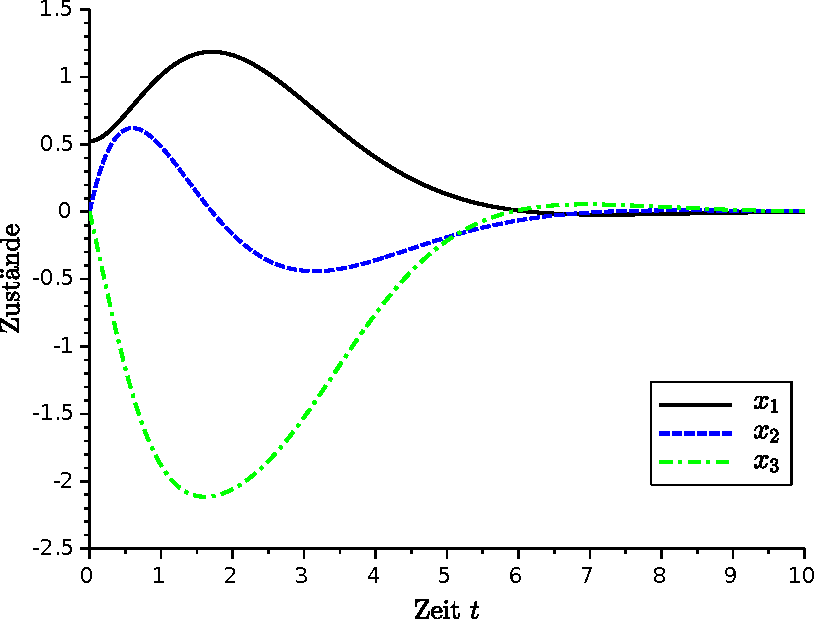
\includegraphics[width=0.8\textwidth]{Inv_Pendel_Motor_LQR}
\par\end{centering}
\caption{Einschwingverhalten des durch LQR-Entwurf in den transformierten Koordinaten
geregelten Pendels\label{fig:opt-inv-pendel-motor-lqr}}

\end{figure}
\end{example}

\subsection{Sontag-Formel}

Die Optimalität des im vorangegangenen Abschnitt hergeleiteten Regelgesetzes~(\ref{eq:opt-LQR-EZ-lin})
hinsichtlich eines quadratischen Gütekriteriums bezieht sich allerdings
nicht auf das Originalsystem~(\ref{eq:basissystem-optimierung}),
sondern auf das transformierte und durch die Rückführung linearisierte
System~(\ref{eq:opt-linearisiertes-system}). In den Originalkoordinaten
ist das Regelgesetz~(\ref{eq:opt-LQR-EZ-lin}) in der Regel keine
Lösung eines Optimierungsproblems\footnote{Die Aussage, dass das Regelgesetz~(\ref{eq:opt-LQR-EZ-lin}) in der
Regel nicht optimal im Sinne eines Kostenfunktionals~(\ref{eq:opt-Kosten-nl})
ist, lässt dadurch veranschaulichen, dass die Rückführung~(\ref{eq:opt-LQR-EZ-lin})
alle im System auftretenden Nichtlinearitäten kompensiert, auch jene,
die die Stabilität begünstigen.} mit einem Kostenfunktional der Form~(\ref{eq:opt-Kosten-nl}). In
diesem Abschnitt wird ein Regelgesetz angegeben, welches das System~(\ref{eq:basissystem-optimierung})
stabilisiert und zugleich Lösung eines Optimierungsproblems ist. Dieser
Zugang ist unter der Bezeichnung \emph{invers-optimale}\index{invers-optimale Regelung}
oder \emph{modifizierte optimale Regelung} \index{modifizierte optimale Regelung}
bekannt~\cite{freeman96control,freeman96siam,freeman1996buch,sepulchre97,sackmann2005modifizierte}.

Zunächst verallgemeinern wir den Begriff der Ljapunov-Funktion auf
Systeme mit Erregung. Sei $V:\R^{n}\to\R$ eine stetig differenzierbare,
positiv definite Funktion (siehe Anhang~\ref{sec:Stabilitaet-autonomer-Systeme}).
Die Funktion~$V$ nennt man \emph{Regelungs-Ljapunov-Funktion}\index{Regelungs-Ljapunov-Funktion}
(engl. \emph{control Lyapunov function}, kurz \emph{CLF}) von System~(\ref{eq:basissystem-optimierung}),
falls
\begin{equation}
\forall x\neq0:\quad\inf_{u}\left(L_{f}V(x)+L_{g}V(x)u\right)<0.\label{eq:CLF-def1}
\end{equation}
Mit der Existenz einer Regelungs-Ljapunov-Funktion gibt es auch eine
stabilisierende Zustandsrückführung~\cite{artstein1983}:
\begin{theorem}
[Theorem von Artstein]\label{thm:Artstein}Man betrachte das System~(\ref{eq:basissystem-optimierung})
mit $f(0)=0$. Ferner sei~$V$ eine Regelungs-Ljapunov-Funktion.
Dann gibt es eine Zustandsrückführung~(\ref{eq:opt-kappa}) derart,
dass $x=0$ eine asymptotisch stabile Ruhelage des geschlossenen Regelkreises
ist.
\end{theorem}
\begin{proofsketch}Sie~$V$ eine Regelungs-Ljapunov-Funktion von
System~(\ref{eq:basissystem-optimierung}). Die Zeitableitung von~$V$
entlang der Systemdynamik von~(\ref{eq:basissystem-optimierung})
hat die Form
\begin{equation}
\begin{array}{ccl}
\dot{V}(x) & = & V^{\prime}(x)\cdot\dot{x}\\
 & = & V^{\prime}(x)\cdot f(x)+g(x)u\\
 & = & L_{f}V(x)+L_{g}V(x)u.
\end{array}\label{eq:opt-Vdot1}
\end{equation}
Bedingung~(\ref{eq:CLF-def1}) bedeutet, dass man den Eingang~$u$
in Abhängigkeit vom Zustand~$x$ immer so wählen kann, dass~$\dot{V}$
negativ definit ist. Damit ist~$V$ eine Ljapunov-Funktion des in
dieser Weise rückgeführten Systems und die Ruhelage $x=0$ ist asymptotisch
stabil.\end{proofsketch}

Die Bedingung~(\ref{eq:CLF-def1}) ist gleichwertig mit 
\begin{equation}
L_{g}V(x)=0\quad\Longrightarrow\quad L_{f}V(x)<0.\label{eq:CLF-def2}
\end{equation}
In den Punkten~$x$, wo die Ableitung~$\dot{V}$ wegen $L_{g}V(x)=0$
nicht über den Eingang~$u$ beeinflusst werden kann, muss das Vektorfeld~$f$
einen Beitrag zur Stabilität liefern.

Kennt man zu einem gegebenen System~(\ref{eq:basissystem-optimierung})
eine Regelungs-Lyapunov-Funktion~$V$, dann stellt die \emph{Sontag-Formel}\index{Sontag-Formel}~\cite{sontag89,sontag98}
\begin{equation}
u=-\kappa(x)=\left\{ \begin{array}{ccc}
-\frac{L_{f}V(x)+\sqrt{\left[L_{f}V(x)\right]^{2}+\left[L_{g}V(x)\right]^{4}}}{L_{g}V(x)} & \text{falls} & L_{g}V(x)\neq0\\
0 & \text{falls} & L_{g}V(x)=0
\end{array}\right.\label{eq:sontag-formel}
\end{equation}
eine stabilisierende Zustandsrückführung~(\ref{eq:opt-kappa}) bereit.
Setzt man~(\ref{eq:sontag-formel}) in das System ein, dann ergibt
sich aus~(\ref{eq:opt-Vdot1}) die Zeitableitung
\[
\dot{V}(x)=\left\{ \begin{array}{ccc}
-\sqrt{\left[L_{f}V(x)\right]^{2}+\left[L_{g}V(x)\right]^{4}} & \text{falls} & L_{g}V(x)\neq0,\\
L_{f}V(x) & \text{falls} & L_{g}V(x)=0.
\end{array}\right.
\]
Dadurch ist~$\dot{V}$ negativ definit und die Ruhelage $x=0$ des
geschlossenen Regelkreis asymptotisch stabil.

Mit der Rückführung~(\ref{eq:sontag-formel}) stabilisiert man nicht
nur das System~(\ref{eq:basissystem-optimierung}), sondern minimiert
auch ein Kostenfunktional~(\ref{eq:opt-Kosten-nl}). Stellt man die
Rückführung~(\ref{eq:opt-LgV-Regelgesetz}) nach der Wichtungsfunktion~$p$
um, so erhält man 
\begin{equation}
p(x)=\frac{1}{2\kappa(x)}\,L_{g}V(x).\label{eq:inv-opt-p}
\end{equation}
Durch Einsetzen dieser Funktion in die Hamilton-Jacobi-Bellman-Gleichung~(\ref{eq:HJB})
bekommt man die zweite Wichtungsfunktion:
\begin{equation}
q(x)=\frac{1}{4p(x)}\left(L_{g}V(x)\right)^{2}-L_{f}V(x).\label{eq:inv-opt-q}
\end{equation}
Damit ist~(\ref{eq:sontag-formel}) die Lösung des durch das Kostenfunktional~(\ref{eq:opt-Kosten-nl})
mit~(\ref{eq:inv-opt-p}) und~(\ref{eq:inv-opt-q}) beschriebenen
Optimierungsproblems. Die zur Stabiliserung herangezogene Regelungs-Ljapunov-Funktion~$V$
ist dann auch die zugehörige Bellman-Funktion. Die unterschiedlichen
Herangehensweisen bei der optimalen bzw. der invers-optimalen Regelung
werden im nachfolgenden Diagramm veranschaulicht:

\[
\begin{CD}
\text{Kostenfunktional} @. \text{Kostenfunktional}\\
@V{\text{Gl.~\eqref{eq:HJB}}}VV @ AA{\text{Gln.~\eqref{eq:inv-opt-p}, \eqref{eq:inv-opt-q}}}A\\
\text{Bellman-Funktion}~V @= \text{Regelungs-Ljapunov-Funktion}~V\\
@V{\text{Gl.~\eqref{eq:opt-LgV-Regelgesetz}}}VV @VV{\text{Gl.~\eqref{eq:sontag-formel}}}V\\
\text{Regelgesetz} @. \text{Regelgesetz}
\end{CD}
\]

Eine wichtige Konsequenz aus der Optimalität der Zustandsrückführung~(\ref{eq:sontag-formel})
ist die Robustheit des so geregelten System~\cite{freeman96control,freeman96siam,sepulchre97}.
Von der Sontag-Formel~(\ref{eq:sontag-formel}) wurden auch zahlreiche
Abwandlungen entwickelt bzw. erprobt~\cite{lin1991,malisoff2000scl,yu2001}.

\medskip{}

In der Regel ist es sehr schwierig, für ein gegebenes System eine
Regelungs-Ljapunov-Funktion zu finden. Ist das System~(\ref{eq:basissystem-optimierung})
eingangs-zustands-linearisierbar, dann kann es durch die Rückführung~(\ref{eq:opt-rueck-linearisierend})
in das lineare System~(\ref{eq:opt-linearisiertes-system}) überführt
werden. Zu diesem System berechnet man für eine gegebene Matrix $Q\succeq0$
und eine Zahl $R>0$ eine positiv definite Lösung $P\succ0$ der algebraischen
Riccati-Gleichung~(\ref{eq:var-opt-ARE}). Damit erhält man in den
transformierten Koordinaten die Bellman-Funktion $\widetilde{V}(\xi)=\xi^{T}P\xi$.
Diese ist zugleich eine Regelungs-Ljapunov-Funktion des linearisierten
Systems~(\ref{eq:opt-linearisiertes-system}), denn über die Rückführung
$v=-k^{T}\xi$ mit~(\ref{eq:var-opt-k}) erhält man eine asymptotisch
stabile Ruhelage $\xi=0$. Daraus ergibt sich in Originalkoordinaten
die Regelungs-Ljapunov-Funktion
\begin{equation}
V(x)=\widetilde{V}(\Phi(x))=\Phi^{T}(x)\,P\,\Phi(x).\label{eq:inv-opt-CLF-EZ}
\end{equation}
Mit der durch die Sontag-Formel~(\ref{eq:sontag-formel}) gegebenen
Rückführung erhält man ein robustes Regelgesetz. 

Bei einem gegebenen System~(\ref{eq:basissystem-optimierung}) lässt
sich das Vorgehen zum Entwurf der beschriebenen invers-optimalen Regelung
folgendermaßen zusammenfassen:
\begin{enumerate}
\item Bestimmung einer Ausgangsabbildung~$h$, für die das System~(\ref{eq:basissystem-optimierung})
den relativen Grad~$n$ besitzt (siehe Abschnitt~\ref{sec:Exakte-Eingangs-Zustands-Linearisierung}).
\item Berechnung der Lie-Ableitungen $L_{f}h(x),\ldots L_{f}^{n-1}h(x)$. 
\item Berechnung einer positiv definiten Lösung~$P$ der algebraischen
Riccati-Gl.~(\ref{eq:var-opt-ARE}) für das linearisierte System~(\ref{eq:opt-linearisiertes-system}),
z.\,B. mit $Q=I$ und $R=1$.
\item Berechnung der Regelungs-Ljapunov-Funktion~(\ref{eq:inv-opt-CLF-EZ})
mit $\xi_{1}=h(x),\ldots,\xi_{n}=L_{f}^{n-1}h(x)$.
\item Berechnung der Lie-Ableitungen $L_{f}V(x)$ und $L_{g}V(x)$.
\item Berechnung der Zustandsrückführung~(\ref{eq:sontag-formel}).
\end{enumerate}

Die Vorgehensweise zur Nutzung der Sontag-Formel~(\ref{eq:sontag-formel})
für eingangs-zustands-linearisierbare Systeme wird an einem Beispiel
vorgestellt:

\begin{example}
Wir betrachten das bereits in Beispiel~\ref{exa:Inverses-Pendel-Motor-LQR}
behandelte inverse Pendel mit Gleichstrommotor. Aus~(\ref{eq:opt-inv-pendel-motor-lie})
liest man die Koordinatentransformation 
\[
\Phi(x)=\left(\begin{array}{c}
h(x)\\
L_{f}h(x)\\
L_{f}^{2}h(x)
\end{array}\right)=\left(\begin{array}{c}
x_{1}\\
x_{2}\\
\frac{-d{\it x_{2}}+mg\ell\sin{\it x_{1}}+K{\it x_{3}}}{J}
\end{array}\right)
\]
ab. Zusammen mit der Matrix~$P$ aus Gl.~(\ref{eq:opt-inv-pendel-motor-P})
erhält man die Regelungs-Ljapunov-Funktion~(\ref{eq:inv-opt-CLF-EZ}),
mit deren Hilfe man die Zustandsrückführung~(\ref{eq:sontag-formel})
angeben kann. Zu Beginn der Simulation wird die Zustandskomponente~$x_{3}$
sehr stark beeinflusst, so dass sie fast unmitelbar von $x_{3}(0)=0$
auf den Wert von ca. $1,09$ übergeht. Bezogen auf die eigentliche
Regelgröße~$x_{1}$ ist im Unterschied zu Beispiel~\ref{exa:Inverses-Pendel-Motor-LQR}
kein Überschwingen zu erkennen.

\begin{figure}
\begin{centering}
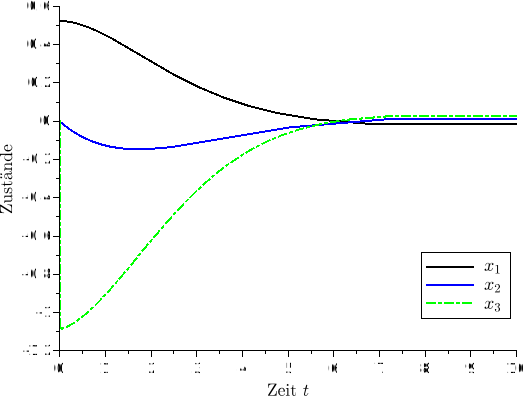
\includegraphics[width=0.8\textwidth]{Inv_Pendel_Motor_Sontag}
\par\end{centering}
\caption{Einschwingverhalten des mit Hilfe der Sontag-Formel geregelten Pendels\label{fig:opt-inv-pendel-motor-sontag}}
\end{figure}
\end{example}
\bibliographystyle{babalpha}
\bibliography{dynamic}




\part{Beobachterentwurf\label{part:Beobachterentwurf}}

\chapter{Beobachter mit großer Verstärkung und starke Beobachter\label{chap:High-Gain-Beobachter}}

Die in den Kapiteln~\ref{chap:regler-grundlagen} und~\ref{chap:regler-varianten}
entworfenen Rückführungen setzen in der Regel die Kenntnis des vollständigen
Systemzustands voraus. In der regelungstechnischen Praxis wird dagegen
meist nur ein Teil der Zustände messtechnisch erfasst. Dieses Kapitel
behandelt einige Ansätze für Zustandsbeobachter, mit denen aus aktuellen
Messdaten von Eingang und Ausgang der jeweilige Systemzustand asymptotisch
rekonstruiert wird. Der Hauptteil des Kapitels befasst sich mit Beobachtern,
bei denen die im System auftretenden Nichtlinearitäten durch eine
lineare Aufschaltung dominiert werden. Zusätzlich wird auf starke
Beobachter eingegangen, welche den Zustand ohne Kenntnis des Systemeingangs
schätzen.

\section{Beobachterentwurf in Originalkoordinaten}

Gegeben sei ein nichtlineares System
\begin{equation}
\dot{x}=F(x,u),\quad y=h(x)\label{eq:hg-system-nicht-affin}
\end{equation}
mit einem eingangsabhängigen Vektorfeld $F:\mathcal{M}\times\mathcal{U}\to\R^{n}$,
der offenen Menge $\mathcal{M}\subseteq\R^{n}$ und dem zulässigen
Wertebereich $\mathcal{U}\subseteq\R^{m}$ der Eingangs\-signale.
Die auf der Menge~$\mathcal{M}$ definierte Abbildung~$h$ überführt
den Zustand~$x$ in die Ausgangsgröße~$y$. Wir gehen davon aus,
dass die Zeitverläufe des Eingangs~$u$ und des Ausgangs~$y$ gemessen
werden. Die Regelung von System~(\ref{eq:hg-system-nicht-affin})
mittels Zustandsrückführung erfordert die Kenntnis des Zustands~$x$.
Da der Ausgang in der Regel eine niedrigere Dimension besitzt als
der Zustand, d.\,h. $\dim y<\dim x$, lässt sich der Zustand~$x$
nicht eindeutig durch eine Umkehrung der Abbildung~$h$ ermitteln.
Stattdessen entwirft man in Ergänzung zu der gegebenen Regelstrecke~(\ref{eq:hg-system-nicht-affin})
ein weiteres dynamisches System, den sogenannten \emph{Beobachter}\index{Beobachter}
bzw. \emph{Zustandsbeobachter} (engl. \emph{state observer}), mit
der allgemeinen Struktur
\begin{equation}
\dot{\hat{z}}=\hat{F}(\hat{z},u,y),\quad\hat{x}=\hat{H}(\hat{z},u,y).\label{eq:hg-beobachter-allgemein}
\end{equation}
Abb.~\ref{fig:beobachter-struktur} skizziert die Verknüpfung von
System und Beobachter. Der Beobachter~(\ref{eq:hg-beobachter-allgemein})
ist so zu entwerfen, dass (ggf. unter zusätzlichen Voraussetzungen
an die Anfangswerte) der geschätzte Zustand~$\hat{x}(t)$ gegen den
Systemzustand~$x(t)$ für $t\to\infty$ konvergiert. In Abhängigkeit
von der Dimension des Zustandsraums des Beobachters~(\ref{eq:hg-beobachter-allgemein})
unterscheidet man zwischen einem \emph{Identitätsbeobachter} ($\dim\hat{z}=\dim x$,
insbesondere $\hat{z}=\hat{x}$), einem \emph{reduzierten Beobachter}\index{Beobachter!reduzierter}
($\dim\hat{z}<\dim x$) sowie einem \emph{Einbettungsbeobachter}\index{Beobachter!Einbettungs-}
($\dim\hat{z}>\dim x$).

Dieser Abschnitt widmet sich dem Entwurf von Beobachtern in den Originalkoordinaten
des Systems. Das dabei entwickelte Entwurfskonzept von Beobachtern
mit großer Verstärkung wird in den Abschnitten~\ref{sec:High-Gain-Entwurf-Beobachtbarkeitsnormalform}
und~\ref{sec:High-Gain-Entwurf-Eingangs-Ausgangs-Normalform} auf
den Beobachterentwurf in den Koordinaten verschiedener Normalformen
übertragen.

\begin{figure}
\begin{centering}
\resizebox{0.6\textwidth}{!}{
\chapter[Beobachterentwurf mittels  Linearisierung der Fehlerdynamik]{Beobachterentwurf mittels exakter bzw. näherungsweiser Linearisierung
der Fehlerdynamik\label{cha:Beobachter-Normalform}}

Normalformen spielen beim Entwurf nichtlinearer Beobachter eine große
Rolle. Kann man ein System in eine Form überführen, bei der die Nichtlinearitäten
ausschließlich von den Messgrößen abhängen, ist der Entwurf eines
Beobachters mit exakt linearer Fehlerdynamik vergleichsweise einfach.
Eine solche Form ist die Beobachternormalform. Die Transformation
in diese Form und damit verbunden die Linearisierung des Beobachtungsfehlers
ist aufgrund restriktiver Existenzbedingungen bzw. einer aufwendigen
Berechnung in der regelungstechnischen Praxis kaum anzutreffen. Bei
genauerer Betrachtung eröffnen sich jedoch etliche Möglichkeiten zur
Berechnung bzw. zur Approximation eines Beobachters mit linearer Fehlerdynamik.
In diesem Kapitel werden Existenzbedingungen und Berechnungsmethoden
vorgestellt.\footnote{Das Kapitel basiert sich an dem Übersichtsbeitrag Röbenack, K.: Entwurf
nichtlinear Beobachter mit linearer und näherungsweise linearer Fehlerdynamik,
Automatisierungstechnik, De Gruyter-Verlag, Berlin, Boston, Jahrgang~58,
Heft~9, S.~489-497, für den der De~Gruyter-Verlag freundlicherweise
eine Nutzungsgenehmigung erteilt hat.}

\section{Linearisierung des Beobachtungsfehlers durch Aufschaltung\label{sec:Linearisierung-durch-Aufschaltung}}

In diesem Abschnitt soll zunächst die grundsätzliche Idee der exakten
Linearisierung des Beobachtungsfehlers durch Aufschaltung illustriert
werden. Angenommen, das zu beobachtende System kann in der Form
\begin{equation}
\dot{x}=Ax+\alpha(y,u),\quad y=c^{T}x\label{eq:lin-beob-fehler-strecke}
\end{equation}
mit dem Zustand~$x$, dem Eingang~$u$, und dem gemessenen Ausgang~$y$
dargestellt werden. Dabei sei der durch das Paar $(A,c^{T})$ beschriebene
lineare Teil beobachtbar. Zusätzlich seien alle auftretenden Nichtlinearitäten
in Abhängigkeit vom Ausgang darstellbar. Diese Nichtlinearitäten werden
in der Eingangs-Ausgangs-Aufschaltung~$\alpha$ zusammengefasst.
Setzt man den Beobachter in der Form
\begin{equation}
\dot{\hat{x}}=A\hat{x}+\alpha(y,u)+l\cdot\left(y-c^{T}\hat{x}\right)\label{eq:lin-beob-fehler-beobachter}
\end{equation}
mit einer Beobachterverstärkung $l\in\R^{n}$ an. so genügt der Beobachtungsfehler
$\tilde{x}=x-\hat{x}$ der linearen zeitinvarianten Differentialgleichung
\begin{equation}
\begin{array}{lcl}
\dot{\tilde{x}} & = & \dot{x}-\dot{\hat{x}}\\
 & = & Ax+\alpha(y,u)-A\hat{x}-\alpha(y,u)-l\cdot\left(y-c^{T}\hat{x}\right)\\
 & = & \left(A-lc^{T}\right)\tilde{x}.
\end{array}\label{eq:lin-beob-fehler-dynamik}
\end{equation}
Über die Verstärkung~$l$ kann man für die Systemmatrix $A-lc^{T}$
der Fehlerdynamik~(\ref{eq:lin-beob-fehler-dynamik}) ein beliebiges
charakteristisches Polynom

\begin{equation}
\det(sI-A+lc^{T})=a_{0}+a_{1}s+\cdots+a_{n-1}s^{n-1}+s^{n}\label{eq:cp}
\end{equation}
vorgeben. Diese Herangehensweise soll an zwei Beispielen vorgestellt
werden:

\begin{example}
\label{exa:inverses-pendel-motor-nf-beobachter}Wir betrachten das
Modell des inversen Pendels mit Gleich\-strom\-antrieb aus Beispiel~\ref{exa:inverses-pendel-gleichstrommotor}:

\begin{equation}
\begin{array}{lcl}
\dot{x}_{1} & = & x_{2}\\
\dot{x}_{2} & = & \frac{mg\ell}{J}\sin x_{1}-\frac{d}{J}x_{2}+\frac{K}{J}x_{3}\\
\dot{x}_{3} & = & -\frac{K}{L}x_{2}-\frac{R}{L}x_{3}+\frac{1}{L}u\\
y & = & x_{1}.
\end{array}\label{eq:inverses-pendel-motor-nf-strecke}
\end{equation}
Als Messgröße steht der Winkel~$x_{1}$, der beispielsweise mit einem
Inkrementgeber erfasst werden kann, zur Verfügung. Die einzige im
System auftretende Nichtlinearität hängt ausschließlich vom Ausgang~$x_{1}$
ab. Der Beobachter setzt sich dann aus einer Kopie des Systems, wobei
die Nichtlinearität vom gemessenen Ausgang gespeist wird, und einem
linearen Korrekturterm zusammen: 
\begin{equation}
\left(\begin{array}{l}
\dot{\hat{x}}_{1}\\
\dot{\hat{x}}_{2}\\
\dot{\hat{x}}_{3}
\end{array}\right)=\left(\begin{array}{c}
\hat{x}_{2}\\
\frac{mg\ell}{J}\sin y-\frac{d}{J}\hat{x}_{2}+\frac{K}{J}\hat{x}_{3}\\
-\frac{K}{L}\hat{x}_{2}-\frac{R}{L}\hat{x}_{3}+\frac{1}{L}u
\end{array}\right)+\left(\begin{array}{l}
l_{1}\\
l_{2}\\
l_{3}
\end{array}\right)\cdot\left(y-\hat{x}_{1}\right)\label{eq:inverses-pendel-motor-nf-beobachter}
\end{equation}
Der Vergleich von~(\ref{eq:inverses-pendel-motor-nf-strecke}) und~(\ref{eq:inverses-pendel-motor-nf-beobachter})
führt auf eine lineare Fehlerdynamik~(\ref{eq:lin-beob-fehler-dynamik}).
Für ein vorgegebenes charakteristisches Polynom~(\ref{eq:cp}) mit
den Koeffizienten $a_{0},a_{1},a_{2}>0$ berechnet man durch Koeffizientenvergleich
oder mit Hilfe der Ackermann-Formel~\cite{acker77,ackermann77} die
Beobachterverstärkung 
\begin{equation}
\begin{array}{lcl}
l_{1} & = & -\frac{R}{L}-\frac{d}{J}+a_{2},\\
l_{2} & = & \frac{-JK^{2}L+\left(a_{1}J^{2}-a_{2}dJ+d^{2}\right)L^{2}-J\left(a_{2}J-d\right)LR+J^{2}R^{2}}{J^{2}L^{2}},\\
l_{3} & = & -\frac{\left(a_{2}J-d\right)K^{2}L^{2}-a_{0}J^{2}L^{3}+JL\left(a_{1}JL-2K^{2}\right)R-a_{2}J^{2}LR^{2}+J^{2}R^{3}}{JKL^{3}}.
\end{array}\label{eq:inverses-pendel-motor-nf-verstaerkung}
\end{equation}
\end{example}

\begin{example}
\label{exa:inverses-pendel-elastisch}Wir betrachten wiederum einen
Manipulator in der Form eines inversen Pendels (siehe Abb.~\ref{fig:Inverses-Pendel-elastisch}).
Der Antrieb erfolgt über ein eingeprägtes Drehmoment~$u$, welches
den Winkel~$q_{1}$ beeinflusst. Der Antrieb ist über eine elastische
Welle, die als Torsionsfeder mit der Federkonstanten~$k$ modelliert
wird, mit dem Manipulatorarm verbunden. Die Position des Manipulatorarms
wird durch den Relativwinkel~$q_{2}$ beschrieben. Der Manipulator
habe beim Antrieb das Trägheitsmoment~$J_{1}$ und hinsichtlich des
Manipulatorarms das Trägheitsmoment~$J_{2}$. Am Ende des Manipulatorarms
der Länge~$\ell$ befinde sich eine Last mit der Masse~$m$.

Das System hat die kinetische Energie
\[
T=\frac{J_{1}}{2}\dot{q}_{1}^{2}+\frac{J_{2}}{2}\left(\dot{q}_{1}+\dot{q}_{2}\right)^{2}
\]
und die potentielle Energie
\[
V=m\ell\left(\cos(q_{1}+q_{2})-1\right)+\frac{k}{2}q_{2}^{2}.
\]
Aus der zugehörigen Bewegungsgleichung erhält man mit $x=(q_{1},\dot{q}_{1},q_{2},\dot{q}_{2})^{T}$
das Zustandsraummodell
\begin{equation}
\left(\begin{array}{l}
\dot{x}_{1}\\
\dot{x}_{2}\\
\dot{x}_{3}\\
\dot{x}_{4}
\end{array}\right)=\left(\begin{array}{c}
x_{2}\\
\frac{k}{J_{1}}x_{3}+\frac{1}{J_{1}}u\\
x_{4}\\
\frac{mg\ell}{J_{2}}\sin(x_{1}+x_{3})-\left(\frac{1}{J_{1}}+\frac{1}{J_{2}}\right)kx_{3}-\frac{u}{J_{1}}
\end{array}\right).\label{eq:inverses-pendel-elastisch}
\end{equation}
Werden die Winkel~$x_{1}$ und~$x_{3}$ oder deren Summe $x_{1}+x_{3}$
gemessen, dann kann die in~(\ref{eq:inverses-pendel-elastisch})
auftretende Nichtlinearität $\sin(x_{1}+x_{3})$ beim Beobachterentwurf
vollständig kompensiert werden~\cite{nicosia88}.
\end{example}
\begin{figure}
\begin{centering}
\resizebox{0.4\textwidth}{!}{\input{inv_pendel_elastisch.pdftex_t}}
\par\end{centering}
\caption{Inverses Pendel, welches elatisch mit dem Antrieb gekoppelt ist\label{fig:Inverses-Pendel-elastisch}}
\end{figure}


\section{Normalfrom-Beobachter\label{sec:Normal-Form-Observer}}

\subsection{Beobachter-Struktur}

Die in Abschnitt~\ref{sec:Linearisierung-durch-Aufschaltung} beschriebene
Herangehensweise wird nachfolgend systematisiert. In der Regel wird
das zu untersuchende System nicht unmittelbar in der Form~(\ref{eq:lin-beob-fehler-strecke})
vorliegen. In etlichen Fällen ist aber eine derartige Darstellung
in anderen Koordinaten möglich. Dazu wird in diesem Abschnitt die
Beobachternormalform eingeführt.

Man betrachte ein nichtlineares System 
\begin{equation}
\dot{x}=F(x,u),\quad y=h(x).\label{eq:plant}
\end{equation}
Die Menge $\mathcal{M}\subseteq\R^{n}$ sei offen und die Menge $\mathcal{U}\subseteq\R^{m}$
beliebig. Die Abbildungen $F:\mathcal{M}\times\mathcal{U}\to\R^{n}$
und $h:\mathcal{M}\to\R$ seien ausreichend glatt. Damit ist~$F$
ein vom Eingang abhängiges Vektorfeld und~$h$ ein Skalarfeld. Angenommen,
in der Umgebung eines Punktes $p\in\mathcal{M}$ gibt es einen Diffeomorphismus
\begin{equation}
z=T(x)\quad\textrm{mit}\quad x=S(z),\label{eq:TS}
\end{equation}
der das System~(\ref{eq:plant}) in die Form 
\begin{equation}
\dot{z}=Az+\alpha(c^{T}z,u),\quad y=\gamma(c^{T}z)\label{eq:nf}
\end{equation}
überführt, wobei das Paar $(A,c^{T})$ in der \emph{dualen} \emph{Brunovský-Normalform}\index{Brunovský-Normalform!duale}\index{Normalform!duale Brunovský-}~\cite{brunovsky70}
vorliege: 
\begin{equation}
A=\left(\begin{array}{cccc}
0 & 0 & \cdots & 0\\
1 & 0 & \ddots & \vdots\\
 & \ddots & \ddots & 0\\
0 &  & 1 & 0
\end{array}\right),\quad c^{T}=\left(\begin{array}{cccc}
0 & \cdots & 0 & 1\end{array}\right).\label{eq:AC}
\end{equation}
Die Form~(\ref{eq:nf}) entspricht der \emph{Beobachter\-normal\-form}
(engl. \emph{observer canonical form})~\cite{zeitz85,zeitz89}\index{Beobachternormalform}\index{Normalform!Beobachter-}
mit der zusätzlichen Ausgangstransformation~$\gamma$ (siehe Abb.~\ref{fig:Beobachter-Normalform}).
Die Abbildung~$\gamma$ muss dabei invertierbar sein. Die vektorwertige
Abbildung~$\alpha$ berücksichtigt die im System auftretenden Nichtlinearitäten.
Dabei fungiert $\alpha(\gamma^{-1}(y),u)$ als Eingangs-Ausgangs-Aufschaltung. 

\begin{figure}
\begin{centering}
\resizebox{0.7\textwidth}{!}{\input{bild-nf2.pdftex_t}}
\par\end{centering}
\caption{Beobachternormalform~(\ref{eq:nf}), Quelle:~\cite{roebenack2010at}\label{fig:Beobachter-Normalform}}
\end{figure}

Für ein System der Form~(\ref{eq:nf}) ist der Beobachterentwurf
sehr einfach. Ein Beobachter der Form 
\begin{equation}
\begin{array}{ccl}
\dot{\hat{z}} & = & A\hat{z}+\alpha(\gamma^{-1}(y),u)+l(\gamma^{-1}(y)-c^{T}\hat{z})\\
\hat{x} & = & S(\hat{z})
\end{array}\label{eq:obs-in-nf}
\end{equation}
mit dem Vektor $l\in\R^{n}$ (siehe Abb.~\ref{fig:Normalform-Beobachter})
führt auf einen Beobachtungsfehler $\tilde{z}=z-\hat{z}$, welcher
dem linearen zeit\-invarianten Differential\-gleichungs\-system
\begin{equation}
\dot{\tilde{z}}=(A-lc^{T})\tilde{z}\label{eq:error-dgl-nf}
\end{equation}
genügt. Da das Paar $(A,c^{T})$ beobachtbar ist, lassen sich die
Eigenwerte von $A-lc^{T}$ beliebig zuweisen. Für ein gewünschtes
charakteristisches Polynom~(\ref{eq:cp}) der Fehlerdynamik~(\ref{eq:error-dgl-nf})
ist der Vektor~$l$ entsprechend $l=(a_{0},\ldots,a_{n-1})^{T}$
zu wählen. Legt man~$l$ derart fest, dass alle Wurzeln von~(\ref{eq:cp})
in der offenen linken Halbebene liegen, dann ist die Ruhelage $\tilde{z}=0$
von~(\ref{eq:error-dgl-nf}) exponentiell (und damit auch asymptotisch)
stabil. 

\begin{figure}
\begin{centering}
\resizebox{0.85\textwidth}{!}{\input{bild-nfbeob1.pdftex_t}}
\par\end{centering}
\caption{Normalform-Beobachter~(\ref{eq:obs-in-nf})\label{fig:Normalform-Beobachter}}
\end{figure}

Der Beobachter~(\ref{eq:obs-in-nf}) basiert unmittelbar auf der
Normalform~(\ref{eq:nf}). Daher nennt man ihn \emph{Normalform-Beobachter}\index{Beobachter!Normalform-}.\index{Normalform-Beobachter}
Mitunter ist es wünschenswert, den Beobachter~(\ref{eq:obs-in-nf})
direkt in den Originalkoordinaten zu implementieren:
\begin{equation}
\dot{\hat{x}}=F(\hat{x},u)+k_{\infty}(\hat{x},y,u).\label{eq:ons-orig}
\end{equation}
Der Korrekturterm hat dann die Form 
\begin{equation}
\begin{array}{ccl}
k_{\infty}(\hat{x},y,u) & = & \left(T^{\prime}(\hat{x})\right)^{-1}\left[\alpha(\gamma^{-1}(y),u)-\alpha(\gamma^{-1}(h(\hat{x})),u)\right.\\
 &  & \left.+\,l(\gamma^{-1}(y)-\gamma^{-1}(h(\hat{x})))\right].
\end{array}\label{eq:correction-term-nf-obs}
\end{equation}

\begin{remark}
Mit dem beschriebenen Zugang ergibt sich eine Fehlerdynamik, die in
den transformierten Koordinaten einer linearen zeit\-invarianten
Differentialgleichung~(\ref{eq:error-dgl-nf}) genügt. Daher spricht
man auch von einer \emph{exakten Linearisierung des Beobachtungsfehlers}.
Dieses Konzept ist auch bei Systemen mit mehreren Ausgängen anwendbar~\cite{krener85observer,xia88,xia89}
und kann mit einer Parameter\-adaption kombiniert werden~\cite{marino1990,marino1992,marino1995,marino1995book}.
Die Linearisierung des Beobachtungsfehlers entspricht in gewisser
Weise der vollständigen Linearisierung (Eingangs-Zustands-Linearisierung)
beim Reglerentwurf. Ähnlich wie bei der Regelung ist auch beim Beobachterentwurf
mitunter nur eine \emph{partielle Linearisierung des Beobachtungsfehlers}
möglich. Entsprechende Entwurfsverfahren werden beispielsweise in~\cite{jo2000b,jo2002,roebenack2005syncod,roebenack2006amcs,roebenack2007iet,roebenack2007ndst}
beschrieben.
\end{remark}

\begin{remark}
Mitunter wird für das System~(\ref{eq:nf}) mit dem Beobachter~(\ref{eq:obs-in-nf})
eine andere Darstellungsform favorisiert. Seien 
\[
\check{A}:=A-lc^{T}\quad\mbox{und}\quad\check{\alpha}(z_{n},u):=\alpha(z_{n},u)+lz_{n},
\]
wobei der Vektor $l\in\R^{n}$ so zu wählen ist, dass die Matrix~$\check{A}$
nur Eigenwerte in der linken offenen Halbebene besitzt. Das System~(\ref{eq:nf})
lässt sich dann in der Form 
\[
\begin{array}{ccl}
\dot{z} & = & Az+\alpha(z_{n},u)\\
 & = & Az-lc^{T}z+lc^{T}z+\alpha(z_{n},u)\\
 & = & \check{A}z+\check{\alpha}(\gamma^{-1}(y),u)
\end{array}
\]
angeben. Der Beobachter~(\ref{eq:obs-in-nf}) vereinfacht sich zu
\[
\begin{array}{ccl}
\dot{\hat{z}} & = & A\hat{z}+\alpha(z_{n},u)+l(z_{n}-c^{T}\hat{z})\\
 & = & (A-lc^{T})\hat{z}+\alpha(z_{n},u)+lz_{n}\\
 & = & \check{A}\hat{z}+\check{\alpha}(\gamma^{-1}(y),u)
\end{array}
\]
mit $\hat{x}=S(\hat{z})$. Als Fehlerdifferentialgleichung erhält
man wiederum Gl.~(\ref{eq:error-dgl-nf}), d.\,h. $\dot{\tilde{z}}=\check{A}\tilde{z}$.
Diese Form von Strecke und Beobachter ist bei verschiedenen neueren
Zugängen zur exakten bzw. approximativen Linearisierung des Beobachtungsfehlers
zu finden (siehe~\cite{kazantzis1998,krener2002,xiao2006,deutscher2006,deutscher2007}
sowie Anmerkung~\ref{rem:Boebachter-mit-Hilfssatz-von-Ljapunov}).
\end{remark}

\begin{remark}
\label{rem:endliche-Einstellzeit}Bei der Fehlerdifferentialgleichung~(\ref{eq:error-dgl-nf})
des Normalformbeobachters~ (\ref{eq:obs-in-nf}) kann man durch geeignete
Wahl des Vektors $l\in\R^{n}$ die Eigenwerte der Systemmatrix $A-lc^{T}$
in der komplexen Ebene beliebig weit links anordnen und damit die
Konvergenzgeschwindigkeit vorgeben. Bei einem Anfangswert $\tilde{z}(0)\neq0$
wird die Ruhelage $\tilde{z}=0$ von~(\ref{eq:error-dgl-nf}) jedoch
erst in unendlicher Zeit erreicht. Für lineare Systeme kann man durch
geeignete Nutzung eines Totzeitgliedes eine endliche Einstellzeit
vorgeben~\cite{engel2002}. Dieser Zugang lässt sich auch für nichtlineare
Systeme, die in die Beobachternormalform~(\ref{eq:nf}) transformierbar
sind, erweitern~\cite{menold2003cdc}.
\end{remark}

\subsection{Reduzierter Normalform-Beobachter}

Bei der Normalform~(\ref{eq:nf}) lässt sich die letzte Komponente
des Zustands mit $z_{n}=\gamma^{-1}(y)$ direkt aus dem Ausgang rekonstruieren
und muss daher nicht geschätzt werden. Folglich ist es naheliegend,
zur Rekonstruktion der verbleibenden $n-1$ Zustandsgrößen $z_{1},\ldots,z_{n-1}$
einen \emph{reduzierten} Beobachter\index{Beobachter!reduzierter}
einzusetzen. 

Die Herleitung eines reduzierten Zustandsbeobachters ist in Analogie
zum linearen Fall möglich~\cite[Abschnitt~{7.4.2}]{ludyk1995-2}.
Durch Streichen der letzten Differentialgleichung in der Normalform~(\ref{eq:nf})
erhält man das System 
\begin{equation}
\dot{\bar{z}}=\bar{A}\bar{z}+\bar{\alpha}(\bar{c}^{T}z,u)\label{eq:reduzierte-nf}
\end{equation}
mit 
\[
\bar{z}=\left(\begin{array}{c}
z_{1}\\
\vdots\\
z_{n-1}
\end{array}\right)\quad\mbox{und}\quad\bar{\alpha}(z_{n},u)=\left(\begin{array}{c}
\alpha_{1}(z_{n},u)\\
\vdots\\
\alpha_{n-1}(z_{n},u)
\end{array}\right).
\]
Das Paar $(\bar{A},\bar{c}^{T})$ mit $\bar{A}\in\R^{(n-1)\times(n-1)}$
und $\bar{c}\in\R^{n-1}$ liegt in der dualen Brunovský-Normalform
der Ordnung $n-1$ vor (siehe Gl.~(\ref{eq:AC})). Der Beobachtungsfehler
$\tilde{\bar{z}}=\bar{z}-\hat{\bar{z}}$ soll einer linearen zeit\-invarianten
Differentialgleichung 
\begin{equation}
\dot{\tilde{\bar{z}}}=\left(\bar{A}-\bar{l}\,\bar{c}^{T}\right)\tilde{\bar{z}}\label{eq:reduziert-error-dgl}
\end{equation}
genügen, wobei der Vektor $\bar{l}=(p_{0},\ldots,p_{n-2})^{T}\in\R^{n-1}$
die Koeffizienten eines vorgegebenen charakteristischen Polynoms vom
Grad $n-1$ enthält. Der Vergleich von~(\ref{eq:reduzierte-nf})
und~(\ref{eq:reduziert-error-dgl}) liefert für den Zustand $\hat{\bar{z}}=\bar{z}-\tilde{\bar{z}}$
die Differentialgleichung
\begin{equation}
\dot{\hat{\bar{z}}}=\bar{A}\hat{\bar{z}}+\bar{\alpha}(z_{n},u)+\bar{l}\tilde{\bar{z}}_{n-1}\label{eq:red-nf-beob-schritt1}
\end{equation}
mit $\tilde{\bar{z}}_{n-1}=\bar{z}_{n-1}-\hat{\bar{z}}_{n-1}$. In
dieser Gleichung wird $\bar{z}_{n-1}=z_{n-1}$ benötigt. Diese Größe
lässt sich aus der letzten Differentialgleichung 
\[
\dot{z}_{n}=z_{n-1}+\alpha_{n}(z_{n},u),\quad z_{n}=\gamma^{-1}(y)
\]
der Normalform~(\ref{eq:nf}) rekonstruieren: 
\[
\bar{z}_{n-1}=z_{n-1}=\frac{\d}{\d t}\left(\gamma^{-1}(y)\right)-\alpha_{n}(\gamma^{-1}(y),u).
\]
Durch Einsetzen in~(\ref{eq:red-nf-beob-schritt1}) erhält man 
\[
\begin{array}{ccl}
\dot{\hat{\bar{z}}} & = & \bar{A}\hat{\bar{z}}+\bar{\alpha}(\gamma^{-1}(y),u)+\bar{l}\left(\frac{\d}{\d t}\left(\gamma^{-1}(y)\right)-\alpha_{n}(\gamma^{-1}(y),u)-\bar{c}^{T}\hat{\bar{z}}\right)\\
 & = & \left(\bar{A}-\bar{l}\,\bar{c}^{T}\right)\hat{\bar{z}}+\bar{\alpha}(\gamma^{-1}(y),u)+\bar{l}\left(\frac{1}{\gamma^{\prime}(y)}\dot{y}-\alpha_{n}(\gamma^{-1}(y),u)\right).
\end{array}
\]
Diese Gleichung kann wegen der auf der rechten Seite auftretenden
Zeit\-ab\-leitung~$\dot{y}$ noch nicht für die Zustandsbeobachtung
eingesetzt werden. Zur Elimination von~$\dot{y}$ wird für den Beobachter
die Koordinatentransformation 
\[
\begin{array}{ccccc}
w & = & \hat{\bar{z}} & - & \bar{l}\gamma^{-1}(y)\\
\hat{\bar{z}} & = & w & + & \bar{l}\gamma^{-1}(y)
\end{array}
\]
eingeführt. Dann gilt 
\[
\begin{array}{ccl}
\dot{w} & = & \frac{\d}{\d t}\left(\hat{\bar{z}}-\bar{l}\gamma^{-1}(y)\right)\\
 & = & \dot{\hat{\bar{z}}}-\bar{l}\frac{\d}{\d t}\left(\gamma^{-1}(y)\right)\\
 & = & \left(\bar{A}-\bar{l}\,\bar{c}^{T}\right)\hat{\bar{z}}+\bar{\alpha}(\gamma^{-1}(y),u)+\bar{l}\left(\frac{\d}{\d t}\left(\gamma^{-1}(y)\right)-\alpha_{n}(\gamma^{-1}(y),u)\right)-\bar{l}\frac{\d}{\d t}\left(\gamma^{-1}(y)\right)\\
 & = & \left(\bar{A}-\bar{l}\,\bar{c}^{T}\right)\hat{\bar{z}}+\bar{\alpha}(\gamma^{-1}(y),u)-\bar{l}\alpha_{n}(\gamma^{-1}(y),u)\\
 & = & \left(\bar{A}-\bar{l}\,\bar{c}^{T}\right)\left(w+\bar{l}\gamma^{-1}(y)\right)+\bar{\alpha}(\gamma^{-1}(y),u)-\bar{l}\alpha_{n}(\gamma^{-1}(y),u)\\
 & = & \left(\bar{A}-\bar{l}\,\bar{c}^{T}\right)w+\left(\bar{A}-\bar{l}\,\bar{c}^{T}\right)\bar{l}\gamma^{-1}(y)+\bar{\alpha}(\gamma^{-1}(y),u)-\bar{l}\alpha_{n}(\gamma^{-1}(y),u).
\end{array}
\]
Die letzte Gleichung liefert den \emph{reduzierten Normalform-Beobachter}\index{Normalform-Beobachter!reduzierter}
\begin{equation}
\dot{w}=\left(\bar{A}-\bar{l}\,\bar{c}^{T}\right)w+\underbrace{\left(\bar{A}-\bar{l}\,\bar{c}^{T}\right)\bar{l}\gamma^{-1}(y)+\bar{\alpha}(\gamma^{-1}(y),u)-\bar{l}\alpha_{n}(\gamma^{-1}(y),u)}_{{\displaystyle \kappa(\gamma^{-1}(y),u)}}\label{eq:red-nf-beob}
\end{equation}
mit dem Korrekturterm~$\kappa$, wobei der Originalzustand mittels
\begin{equation}
\hat{z}=\left(\begin{array}{c}
w+\bar{l}\gamma^{-1}(y)\\
\gamma^{-1}(y)
\end{array}\right),\quad\hat{x}=S(\hat{z})\label{eq:red-nf-ruecktransf}
\end{equation}
rekonstruiert wird. Das zugehörige Strukturbild ist in Abb.~\ref{fig:Reduzierter-Normalformbeobachter}
dargestellt.

\begin{figure}
\begin{centering}
\resizebox{0.85\textwidth}{!}{\input{bild-reduzierter-nf-beob1.pdftex_t}}
\par\end{centering}
\caption{Reduzierter Normalformbeobachter~(\ref{eq:red-nf-beob}) mit Rücktransformation~(\ref{eq:red-nf-ruecktransf})\label{fig:Reduzierter-Normalformbeobachter}}
\end{figure}


\section{Existenz und Berechnung der Beobachternormalform}

\subsection{Existenz und Berechnung der Normalform nach Byrnes und Isidori\label{subsec:Berechnung-nach-Byrnes-Isidori}}

Die Schwierigkeit beim Entwurf eines Normalform-Beobachters besteht
in der Existenz der Normalform~(\ref{eq:nf}) sowie in der konkreten
Berechnung der Transformation~(\ref{eq:TS}). Für die folgenden Betrachtungen
ist es zweckmäßig, das zu beobachtende System~(\ref{eq:plant}) in
der Form 
\begin{equation}
\dot{x}=f(x)+g(x,u),\quad y=h(x),\label{eq:plant-fg}
\end{equation}
mit den Abbildungen $f:\mathcal{M}\to\R^{n}$ und $g:\mathcal{M}\times\mathcal{U}\to\R^{n}$
anzugeben. Diese Abbildungen seien durch 
\[
f(x)=F(x,0)\quad\mbox{und}\quad g(x,u)=F(x,u)-F(x,0)
\]
festgelegt. Die Beobachtbarkeitsmatrix\index{Beobachtbarkeitsmatrix}~$Q_{B}$
ist die Jacobimatrix der Beobachtbarkeitsabbildung\index{Beobachtbarkeitsabbildung}~$q:\mathcal{M}\to\R^{n}$,
d.\,h. 
\begin{equation}
q(x)=\left(\begin{array}{c}
h(x)\\
L_{f}h(x)\\
\vdots\\
L_{f}^{n-1}h(x)
\end{array}\right),\quad Q_{B}(x)=q^{\prime}(x)=\left(\begin{array}{c}
dh(x)\\
L_{f}dh(x)\\
\vdots\\
L_{f}^{n-1}dh(x)
\end{array}\right),\label{eq:Q}
\end{equation}
vgl. Abschnitt~\ref{subsec:Beobachtbarkeit-autonom}. Der sogenannte
\emph{Start\-vektor} bzw. das sog. \emph{Start\-vektor\-feld}\index{Startvektorfeld}\footnote{Mit dem Vektorfeld~$v$ wird zyklisch der gesamte Raum für das transformierte
System aufgespannt.} ist die Lösung des Gleichungssystems
\begin{equation}
Q_{B}(x)\,v(x)=\beta(h(x))\,\frac{\partial}{\partial x_{n}}\label{eq:v}
\end{equation}
mit einer skalarwertigen Funktion~$\beta$. Der folgende Satz gibt
die Existenzbedingungen für die Normalform~(\ref{eq:nf}) an~\cite{krener83,marino1990}:
\begin{theorem}
\label{thm:existence}In einer Umgebung von $p\in\mathcal{M}$ existiert
genau dann ein lokaler Diffeomorphismus~(\ref{eq:TS}), der das System~(\ref{eq:plant-fg})
in die Normalform~(\ref{eq:nf}) mit einem lokalen Diffeomorphismus~$\gamma$
überführt, wenn für eine geeignete Funktion~$\beta$ mit $\beta(h(p))\neq0$
die Bedingungen
\begin{enumerate}
\item \label{enu:ki1}$\rank\,Q_{B}(p)=n$

\item \label{enu:ki2}$[\ad_{-f}^{i}v,\ad_{-f}^{j}v](x)=0$ für $0\leq i,j\leq n-1$
\item \label{enu:ki3}$[g,\ad_{-f}^{i}v](x,u)=0$ für $0\leq i\leq n-2$
\end{enumerate}
für alle $x$ in einer Umgebung von~$p$ und für alle $u\in\mathcal{U}$
erfüllt sind. Es gibt einen globalen Diffeomrophismus~(\ref{eq:TS}),
wenn die Bedingungen~\ref{enu:ki1}-\ref{enu:ki3} in $\mathcal{M}=\R^{n}$
gelten und zusätzlich
\begin{enumerate}[start=4]
\item \label{enu:ki4}$\ad_{-f}^{i}v$ für $0\leq i<n$ vollständige Vektorfelder\index{Vektorfeld!vollständiges}
sind.
\end{enumerate}
\end{theorem}
Der folgende Beweis widmet sich der Existenz einer lokalen Koordinatentransformation. 
\begin{svmultproof2}
\hinreichend\ Die Bedingungen \ref{enu:ki1}-\ref{enu:ki3} seien
in einer Umgebung von $p\in\mathcal{M}$ erfüllt. Wegen Bedingung~\ref{enu:ki1}
ist das lineare Gls.~(\ref{eq:v}) (eindeutig) lösbar bezüglich~$v$.
Zeilenweise kann man Gls.~(\ref{eq:v}) auch in der Form 
\begin{equation}
L_{v}L_{f}^{i}h(x)=\left\langle \d L_{f}^{i}h(x),v(x)\right\rangle =\left\{ \begin{array}{ccl}
0 & \mbox{für} & i=0,\ldots,n-2,\\
\beta(h(x)) & \mbox{für} & i=n-1.
\end{array}\right.\label{eq:proof-obsnf-gl0}
\end{equation}
schreiben. Wegen 
\begin{equation}
\begin{array}{l}
\left(\begin{array}{c}
\d h(p)\\
\vdots\\
\d L_{f}^{n-1}h(p)
\end{array}\right)\left(v(p),\,\ad_{-f}v(p),\,\cdots,\,\ad_{-f}^{n-1}v(p)\right)=\\
=\left(\begin{array}{cccc}
0 & \cdots & 0 & \beta(h(p))\\
\vdots & \qdots & \qdots & *\\
0 & \qdots & \qdots & \vdots\\
\beta(h(p)) & * & \cdots & *
\end{array}\right)
\end{array}\label{eq:proof-obsnf-gl1}
\end{equation}
sind die Vektorfelder $v,\ad_{-f}v,\ldots,\ad_{-f}^{n-1}v$ in einer
Umgebung von~$p$ linear unabhängig (vgl. Lemma~\ref{lem:Lin-Unabh-Kovektoren}).
In Verbindung mit Bedingung~\ref{enu:ki2} garantiert der Begradigungssatz
(Satz~\ref{thm:simultane-begradigung-von-VF}) die Existenz eines
lokalen Diffeomorphismus~(\ref{eq:TS}) mit 
\begin{equation}
T_{*}\ad_{-f}^{i}v=\frac{\partial}{\partial z_{i+1}}\quad\mbox{für}\quad i=0,\ldots,n-1.\label{eq:proof-obsnf-gl2}
\end{equation}
 Der Diffeomorphismus~(\ref{eq:TS}) transformiert die im System~(\ref{eq:plant-fg})
auftretenden Abbildungen in die Form 
\begin{equation}
\begin{array}{lcl}
\bar{f}(z) & = & T_{*}f(S(z)),\\
\bar{g}(z,u) & = & T_{*}g(S(z),u),\\
\bar{h}(z) & = & h(S(z)).
\end{array}\label{eq:proof-obsnf-bar-groessen}
\end{equation}
Wegen Gls.~(\ref{eq:proof-obsnf-gl1}) gilt
\begin{equation}
\frac{\partial}{\partial z_{i+1}}\bar{h}=\left\langle \d h,\ad_{-f}^{i}v\right\rangle =\left\{ \begin{array}{ccl}
0 & \mbox{für} & i=0,\ldots,n-2,\\
\beta(h(x)) & \mbox{für} & i=n-1,
\end{array}\right.\label{eq:proof-obsnf-dh-beta}
\end{equation}
d.\,h. der Gradient von~$\bar{h}$ hat die Form 
\[
\bar{h}^{\prime}(z)=\left(\begin{array}{cccc}
0 & \cdots & 0 & *\end{array}\right).
\]
Folglich hat die Ausgangsabbildung~$\bar{h}$ die in Gl.~(\ref{eq:nf})
angegebene Form d.\,h. es besteht nur eine Abhängigkeit von der letzten
Zustandskomponente~$z_{n}$.

Als nächstes wird das Vektorfeld 
\[
\bar{f}=\bar{f}_{1}\frac{\partial}{\partial z_{1}}+\cdots+\bar{f}_{n}\frac{\partial}{\partial z_{n}}
\]
betrachtet. Mit~(\ref{eq:proof-obsnf-gl2}) gilt 
\[
\begin{array}{ccl}
\tfrac{\partial}{\partial z_{i+1}} & = & T_{*}\ad_{-f}^{i}v\\
 & = & T_{*}[-f,\ad_{-f}^{i-1}v]\\
 & = & [-T_{*}f,T_{*}\ad_{-f}^{i-1}v]\\
 & = & [-\bar{f},\tfrac{\partial}{\partial z_{i}}]\\
 & = & \sum_{j=1}^{n}\left(\left(\tfrac{\partial}{\partial z_{i}}\bar{f}_{j}\right)\tfrac{\partial}{\partial z_{j}}\right)
\end{array}
\]
für $i=1,\ldots,n-1$. Ein Vergleich beider Seiten der Gleichung liefert
\[
\frac{\partial\bar{f}_{j}}{\partial z_{i}}=\left\{ \begin{array}{ccccc}
0 & \mbox{für} & j & \neq & i+1\\
1 & \mbox{für} & j & = & i+1
\end{array}\right.
\]
mit $1\leq i\leq n-1$ und $1\leq j\leq n$. Die $n\times n$-Jacobimatrix
von~$\bar{f}$ hat folglich die Form 
\begin{equation}
\bar{f}^{\prime}(z)=\left(\begin{array}{ccccc|c}
0 & 0 & \cdots & 0 & 0 & *\\
1 & 0 &  & \vdots & 0 & *\\
0 & 1 & \ddots & \vdots & \vdots & \vdots\\
\vdots & 0 & \ddots & 0 & \vdots & \vdots\\
0 & \vdots & \ddots & 1 & 0 & *\\
0 & 0 & \cdots & 0 & 1 & *
\end{array}\right).\label{eq:proof-obsnf-Form-DF}
\end{equation}

Bei dem vom Eingang abhängigen Vektorfeld~$\bar{g}$ geht man ähnlich
vor. Wegen Bedingung~\ref{enu:ki3} und Gl.~(\ref{eq:proof-obsnf-gl2})
gilt 
\[
\begin{array}{ccl}
0 & = & T_{*}[g,\ad_{-f}^{i}v]\\
 & = & [T_{*}g,T_{*}\ad_{-f}^{i}v]\\
 & = & [\bar{g},\frac{\partial}{\partial z_{i+1}}]\\
 & = & -\sum_{j=1}^{n}\left(\left(\tfrac{\partial}{\partial z_{i+1}}\bar{g}_{j}\right)\tfrac{\partial}{\partial z_{j}}\right)
\end{array}
\]
für $i=0,\ldots,n-2$, d.\,h. 
\[
\frac{\partial}{\partial z_{i+1}}\bar{g}_{j}=0\quad\mbox{für}\quad1\leq j\leq n\quad\mbox{und}\quad0\leq i\leq n-2.
\]
Die Jacobimatrix von~$\bar{g}$ hat somit die Form 
\begin{equation}
\frac{\partial\bar{g}}{\partial z}(z,u)=\left(\begin{array}{ccc|c}
0 & \cdots & 0 & *\\
\vdots & \ddots & \vdots & \vdots\\
0 & \cdots & 0 & *
\end{array}\right).\label{eq:proof-obsnf-Form-DG}
\end{equation}
Aus Gln.~(\ref{eq:proof-obsnf-Form-DF}) und~(\ref{eq:proof-obsnf-Form-DG})
folgt, dass das kombinierte Vektorfeld $(\bar{f}+\bar{g})$ die in
Gl.~(\ref{eq:nf}) angegebene Gestalt besitzt.

\notwendig\ Angenommen, es gäbe lokale Diffeomorphismen~(\ref{eq:TS})
und~$\gamma$, die das System~(\ref{eq:plant}) in einer Umgebung
des Punktes~$p$ in die Normalform~(\ref{eq:nf}) überführen. Simultan
wird für das transformierte System~(\ref{eq:nf}) auch die Form~(\ref{eq:proof-obsnf-bar-groessen})
verwendet. Ohne Einschränkung sei $T(p)=0$ (andernfalls Verschiebung
des Koordinatensystems). Die Beobachtbarkeitsmatrix der Normalform
lässt sich leicht berechnen. Zu der Beobachtbarkeitsmatrix~(\ref{eq:Q})
in den Originalkoordinaten besteht folgender Zusammenhang: 
\begin{equation}
\begin{array}{rcl}
Q_{B}(x) & = & {\displaystyle \frac{\partial}{\partial x}}\left(\begin{array}{c}
h(x)\\
\vdots\\
L_{f}^{n-1}h(x)
\end{array}\right)\\
 & = & {\displaystyle \frac{\partial}{\partial z}}\left(\begin{array}{c}
h(S(z))\\
\vdots\\
L_{f}^{n-1}h(S(z))
\end{array}\right){\displaystyle \frac{\partial z}{\partial x}}\\
 & = & {\displaystyle \frac{\partial}{\partial z}}\left(\begin{array}{c}
\bar{h}(z)\\
\vdots\\
L_{\bar{f}}^{n-1}\bar{h}(z)
\end{array}\right){\displaystyle \frac{\partial z}{\partial x}}\\
 & = & \left.\left(\begin{array}{cccc}
0 & \cdots & 0 & \gamma^{\prime}(z_{n})\\
\vdots & \qdots & \qdots & *\\
0 & \qdots & \qdots & \vdots\\
\gamma^{\prime}(z_{n}) & * & \cdots & *
\end{array}\right)\right|_{z=T(x)}\cdot T^{\prime}(x).
\end{array}\label{eq:proof-obnf-Qx-Qz}
\end{equation}
Die Matrizen auf der rechten Seite sind im Punkt~$p$ regulär, weil~$\gamma$
und~$T$ Diffeomorphismen sind. Damit muss auch die Matrix $Q_{B}(p)$
regulär sein, d.\,h. Bedingung~\ref{enu:ki1} ist erfüllt. 

Als nächstes transformieren wir das Vektorfeld~$v$ mittels Pushforward
in die Normalform-Koordinaten: 
\[
\bar{v}(z)=T_{*}v(S(z)).
\]
In den Originalkoordinaten kann das in Gl.~(\ref{eq:v}) definierte
Startvektorfeld auch als Lösung von Gl.~(\ref{eq:proof-obsnf-gl0})
beschrieben werden. Mit Gl.~(\ref{eq:proof-obnf-Qx-Qz}) erhält man
analog in den transformierten Koordinaten die Darstellung 
\[
L_{\bar{v}}L_{\bar{f}}^{i}\bar{h}(z)=\left\langle \d L_{\bar{f}}^{i}\bar{h}(z),\bar{v}(z)\right\rangle =\left\{ \begin{array}{ccl}
0 & \mbox{für} & i=0,\ldots,n-2,\\
\gamma^{\prime}(z_{n}) & \mbox{für} & i=n-1.
\end{array}\right.
\]
Daraus folgt $\beta(h(p))=\gamma^{\prime}(0)\neq0$, so dass die Ausgangstransformation~$\gamma$
ein lokaler Diffeomorphismus ist. Für die Normalform~(\ref{eq:nf})
lässt sich unmittelbar nachrechnen, dass die Bedingungen 
\[
\begin{array}{rclcl}
[\ad_{-\bar{f}}^{i}\bar{v},\ad_{-\bar{f}}^{j}\bar{v}](z) & = & 0 & \mbox{für} & 0\leq i,j\leq n-1\\{}
[\bar{g},\ad_{-\bar{f}}^{i}\bar{v}](z,u) & = & 0 & \mbox{für} & 0\leq i\leq n-2
\end{array}
\]
in einer Umgebung von $z=0$ und für alle $u\in\mathcal{U}$ erfüllt
sind. Aus Proposition~\ref{pro:Lie-Klammer-und-Push-Forward} folgt,
dass die zugehörigen Bedingungen~\ref{enu:ki2} und~\ref{enu:ki3}
auch in den Originalkoordinaten erfüllt sind.
\end{svmultproof2}

Bedingung~\ref{enu:ki1} aus Satz~\ref{thm:existence} ist die lokale
Beobachtbarkeitsbedingung (siehe Abschnitt~\ref{subsec:Beobachtbarkeit-autonom}
und Anmerkung~\ref{rem:stetige-Beobachter}). Die Integrabilitätsbedingung\index{Integrabilitätsbedingung}~\ref{enu:ki2}
ist bei vielen Systemen nicht erfüllt. Allerdings kann man die Klasse
der in die Normalform~(\ref{eq:nf}) transformierbaren Systeme vergrößern,
indem man z.\,B. Zeitskalierungen berücksichtigt~\cite{guay2002,respondek2004}\@.
Bei autonomen Systemen entfällt die Bedingung~\ref{enu:ki3}. 

Selbst wenn die Bedingungen von Satz~\ref{thm:existence} erfüllt
sind, ist die konkrete Berechnung der Normalform~(\ref{eq:nf}) bzw.
des Beobachters~(\ref{eq:ons-orig}) in der Regel sehr schwierig.
Prinzipiell lässt sich dabei wie folgt vorgehen: Ausgehend von der
Beobachtbarkeitsmatrix~(\ref{eq:Q}) bestimmt man den Startvektor~$v$
entsprechend Gl.~(\ref{eq:v}) und die Lie-Klammern $\ad_{-f}v,\ldots,\ad_{-f}^{n-1}v$
für eine geeignete Abbildung~$\beta$. Die Abbildung~$\beta$ ist
dabei so zu wählen, dass Bedingung~\ref{enu:ki2} des Satzes erfüllt
ist. Anschließend fasst man die vektorwertigen Gln.~(\ref{eq:proof-obsnf-gl2})
spaltenweise zu der matrixwertigen Gleichung 
\begin{equation}
I=T^{\prime}(x)\cdot\Pi(x)\label{eq:pde-T}
\end{equation}
mit
\begin{equation}
\Pi(x)=\left(\begin{array}{cccc}
v(x) & \ad_{-f}v(x) & \cdots & \ad_{-f}^{n-1}v(x)\end{array}\right)\label{eq:PI}
\end{equation}
zusammen~\cite{schaffner99}. Die Matrix~$\Pi$ ist dabei die von
den Vektorfeldern~$f$ und~$v$ erzeugte Steuerbarkeitsmatrix (siehe
Anmerkung~\ref{rem:Steuerbarkeitsmatrix}). Bei Gl.~(\ref{eq:pde-T})
handelt es sich um eine partielle Differentialgleichung, die bezüglich~$T$
zu lösen ist. In \textsc{Maple} steht dazu die Routine \texttt{pdesolve}
aus der Bibliothek \texttt{PDEtools} zur Verfügung~\cite{chep-terrab1995}. 

Alternativ kann man die gesuchte Koordinatentransformation~(\ref{eq:TS})
auch unmittelbar auf Basis des im Beweis von Satz~\ref{thm:existence}
verwendeten Begradigungssatzes berechnen. Dazu bestimmt man die Flüsse
der in Gl.~(\ref{eq:PI}) auftretenden Vektor\-felder und bildet
die nachfolgende Flussverknüpfung\index{Fluss!Verkettung} (siehe
Beweis von Satz~\ref{thm:simultane-begradigung-von-VF}):
\begin{equation}
x=S(z)=\varphi_{z_{1}}^{v}\circ\varphi_{z_{2}}^{\ad_{-f}v}\circ\cdots\circ\varphi_{z_{n}}^{\ad_{-f}^{n-1}v}(p).\label{eq:verknuepfung-der-fluesse}
\end{equation}
Mit zunehmender Ordnung der Lie-Klammern werden die Vektor\-felder
$v,ad_{-f}v,\ldots,ad_{-f}^{n-1}v$ in der Regel komplizierter. Bei
dem potentiell kompliziertesten Vektor\-feld $ad_{-f}^{n-1}v$ benötigt
man jedoch nicht den allgemeinen Fluss, sondern nur die Lösung einer
Anfangswertaufgabe, die sich durch geeignete Wahl des Anfangswertes~$p$
oft vereinfachen lässt. Die Umkehrung von~$S$ liefert die Hintransformation~$T$.

Aus der Kenntnis der Transformation~(\ref{eq:TS}) erhält man die
Normalform~(\ref{eq:nf}) bzw. die Abbildungen~$\alpha$ und~$\gamma$
mit Hilfe von Gl.~(\ref{eq:proof-obsnf-bar-groessen}), d.\,h. 
\[
Az+\alpha(z_{n},u)=T_{*}F(S(z))=\left(S^{\prime}(z)\right)^{-1}F(S(z))\quad\mbox{und}\quad\gamma(z_{n})=h(S(z)).
\]
Zwischen den Funktionen~$\beta$ und~$\gamma$ besteht wegen Gl.~(\ref{eq:proof-obsnf-dh-beta})
der Zusammenhang 
\begin{equation}
\gamma^{\prime}(z_{n})=\beta(h(x))=\beta(h(S(z))).\label{eq:dgamma-beta}
\end{equation}
Die Ausgangstransformation~$\gamma$ lässt sich daher bis auf eine
Integrationskonstante durch 
\[
\gamma(z_{n})=\int\beta(h(S(z)))\,\d z_{n}
\]
bestimmen.

\begin{example}
\label{exa:van-der-Pol-Krener-Isidori}Man betrachte den van der Pol-Oszillator
\begin{equation}
\begin{array}{lcl}
\dot{x}_{1} & = & x_{2}\\
\dot{x}_{2} & = & -x_{1}+x_{2}(1-x_{1}^{2})+x_{1}u\\
y & = & x_{1}
\end{array}\label{eq:vdp}
\end{equation}
mit dem zusätzlichen Eingang~$u$ und dem Ausgang~$y$. Das van
der Pol-System~(\ref{eq:vdp}) wird in der Schaltungstechnik häufig
zur Beschreibung von Relaxationsschwingungen in Oszillatoren verwendet~\cite{van-der-pol1926,guckenheimer83,prochaska2004}.
Für $u=0$ enthält die Phasenebene eine instabile Ruhelage im Ursprung
und einen stabilen Grenzzyklus (siehe Abb.~\ref{fig:Phasenportrait-vdP}).
\end{example}
\begin{figure}
\begin{centering}
\resizebox{0.85\textwidth}{!}{\input{vdp-sim.pdftex_t}}
\par\end{centering}
\caption{Phasenebene des van der Pol-Oszillators~(\ref{eq:vdp}) für $u=0$\label{fig:Phasenportrait-vdP}}
\end{figure}

Die zum System gehörende Beobachtbarkeitsmatrix ist die Einheitsmatrix.
Dadurch ergibt sich der Startvektor nach Gl.~(\ref{eq:v}) und die
daraus berechnete Lie-Klammer:
\begin{equation}
v(x)=\left(\begin{array}{c}
0\\
\beta(x_{1})
\end{array}\right),\quad\ad_{-f}v(x)=\left(\begin{array}{c}
\beta(x_{1})\\
\left(1-x_{1}^{2}\right)\beta(x_{1})+x_{2}\beta^{\prime}(x_{1})
\end{array}\right).\label{eq:vdp-Lie-Klammern1}
\end{equation}
Zur Überprüfung der Bedingung~\ref{enu:ki2} aus Satz~\ref{thm:existence}
betrachten wir die weitere Lie-Klammer
\[
[v,\ad_{-f}v](x)=\left(\begin{array}{c}
0\\
-2\beta(x_{1})\beta^{\prime}(x_{1})
\end{array}\right).
\]
Diese Lie-Klammer ist genau dann die Nullfunktion, wenn~$\beta$
konstant ist. Mit $\beta(x_{1})\equiv1$ ist auch die Bedingung~\ref{enu:ki3}
erfüllt, d.\,h. $[g,v]=0$. Die Lie-Klammern~(\ref{eq:vdp-Lie-Klammern1})
vereinfachen sich zu 
\begin{equation}
v(x)=\left(\begin{array}{c}
0\\
1
\end{array}\right)\quad\text{und}\quad\ad_{-f}v(x)=\left(\begin{array}{c}
1\\
1-x_{1}^{2}
\end{array}\right).\label{eq:vdp-Lie-Klammern2}
\end{equation}
Zu diesen Vektorfeldern berechnet man die Flüsse
\[
\varphi_{z_{1}}^{v}(x)=\left(\begin{array}{c}
x_{1}\\
x_{2}+z_{1}
\end{array}\right)\quad\text{und}\quad\varphi_{z_{2}}^{\ad_{-f}v}(x)=\left(\begin{array}{c}
x_{1}+z_{2}\\
x_{2}+(1-x_{1}^{2})z_{2}-x_{1}z_{2}^{2}-\frac{1}{3}z_{2}^{3}
\end{array}\right).
\]
Aus der Flussverkettung~(\ref{eq:verknuepfung-der-fluesse}) erhält
man für $p=(0,0)^{T}$ die Rücktransformation 
\[
\left(\begin{array}{l}
x_{1}\\
x_{2}
\end{array}\right)=S(z)=\varphi_{z_{1}}^{v}\circ\varphi_{z_{2}}^{\ad_{-f}v}(p)=\left(\begin{array}{c}
z_{2}\\
z_{1}+z_{2}-\frac{1}{3}z_{2}^{3}
\end{array}\right).
\]
Die zugehörige Hintransformation lautet
\begin{equation}
\left(\begin{array}{l}
z_{1}\\
z_{2}
\end{array}\right)=T(x)=\left(\begin{array}{c}
x_{2}-x_{1}+\frac{1}{3}x_{1}^{3}\\
x_{1}
\end{array}\right).\label{eq:vdp-hintransformation}
\end{equation}
Durch Anwendung dieser Transformation auf System~(\ref{eq:vdp})
erhält man die Beobachternormalform
\begin{equation}
\left(\begin{array}{l}
\dot{z}_{1}\\
\dot{z}_{2}
\end{array}\right)=\underbrace{\left(\begin{array}{cc}
0 & 0\\
1 & 0
\end{array}\right)}_{{\displaystyle A}}\left(\begin{array}{l}
z_{1}\\
z_{2}
\end{array}\right)+\underbrace{\left(\begin{array}{c}
uz_{2}-z_{2}\\
z_{2}-\frac{1}{3}z_{2}^{3}
\end{array}\right)}_{{\displaystyle \alpha(z_{n},u)}},\quad y=z_{2}.\label{eq:vdp-beobachternormalform}
\end{equation}
Daraus ergibt sich unmittelbar der Normalform-Beobachter
\begin{eqnarray*}
\left(\begin{array}{l}
\dot{\hat{z}}_{1}\\
\dot{\hat{z}}_{2}
\end{array}\right) & = & \left(\begin{array}{cc}
0 & 0\\
1 & 0
\end{array}\right)\left(\begin{array}{l}
\hat{z}_{1}\\
\hat{z}_{2}
\end{array}\right)+\left(\begin{array}{c}
uy-y\\
y-\frac{1}{3}y
\end{array}\right)+\left(\begin{array}{l}
a_{0}\\
a_{1}
\end{array}\right)(y-\hat{z}_{2})\\
\hat{x} & = & S(\hat{z})
\end{eqnarray*}
nach Gl.~(\ref{eq:obs-in-nf}), wobei das charakteristische Polynom~(\ref{eq:cp})
der Fehlerdynamik~(\ref{eq:error-dgl-nf}) über die Koeffizienten
$a_{0},a_{1}>0$ vorgegeben wird. Mit Kenntnis der Koordinatentransformation
und der Eingangs-Ausgangs-Aufschaltung kann man den Beobachter auch
in den Originalkoordianten implementieren. Der zum Beobachter~(\ref{eq:ons-orig})
gehörende Korrekturterm~(\ref{eq:correction-term-nf-obs}) lautet:
\begin{equation}
\begin{array}{lcl}
k_{\infty}(\hat{x},y,u) & = & \left(\begin{array}{cc}
0 & 1\\
1 & 1-\hat{x}_{1}^{2}
\end{array}\right)\left(\left(\begin{array}{c}
uy-y\\
y-\frac{1}{3}y^{3}
\end{array}\right)\!-\!\left(\begin{array}{c}
u\hat{x}_{1}-\hat{x}_{1}\\
\hat{x}_{1}-\frac{1}{3}\hat{x}_{1}^{3}
\end{array}\right)+\left(\begin{array}{c}
a_{0}\\
a_{1}
\end{array}\right)(y-\hat{x}_{1})\right)\end{array}\!.\label{eq:vdp-kinf}
\end{equation}

\begin{example}
\label{exa:Roessler-Krener-Isidori}Man betrachte das Rössler-System~\cite{roessler76,roessler79}
\begin{equation}
\begin{array}{lcl}
\dot{x}_{1} & = & -x_{2}-x_{3}\\
\dot{x}_{2} & = & x_{1}+ax_{2}\\
\dot{x}_{3} & = & c+x_{3}(x_{1}-b)
\end{array}\label{eq:roessler-attraktor}
\end{equation}
mit den Parametern $a,b,c>0$ und der Ausgangsgleichung 
\begin{equation}
y=x_{3}.\label{eq:roessler-ausgang1}
\end{equation}
System~(\ref{eq:roessler-attraktor}) besitzt für bestimmte Anfangs-
und Parameterwerte einen chaotischen Attraktor~\cite{jetschke89,arrowsmith90}.

Für den Ausgang~(\ref{eq:roessler-ausgang1}) erhält man die Beobachtbarkeitsmatrix
\[
Q_{B}(x)=\left(\begin{array}{ccc}
0 & 0 & 1\\
x_{3} & 0 & x_{1}-b\\
c+2x_{3}(x_{1}-b) & \;-x_{3}\; & -x_{2}-2x_{3}+(x_{1}-b)^{2}
\end{array}\right).
\]
Mit Gl.~(\ref{eq:v}) berechnet man das Startvektorfeld~$v$ mit
einem noch nicht festgelegten Skalarfeld~$\beta$, welches wegen
Gl.~(\ref{eq:roessler-ausgang1}) von~$x_{3}$ abhängt:
\[
v(x)=\left(\begin{array}{c}
0\\
-\frac{\beta(x_{3})}{x_{3}}\\
0
\end{array}\right).
\]
Dieser Teil der Berechnungen lässt sich ohne Schwierigkeiten mit \textsc{Maxima}
nachvollziehen, wobei auf die in Alg.~\ref{alg:Berechnung-Beobachtbarkeitsmatrix}
definierte Routine zur Berechnung der Beobachtbarkeitsmatrix zurückgegriffen
wird:

\begin{maxima}\noindent
%%%%%%%%%%%%%%%
%%% INPUT:
\begin{minipage}[t]{8ex}\color{red}\bf
\begin{verbatim}
(%i7) 
\end{verbatim}
\end{minipage}
\begin{minipage}[t]{\textwidth}\color{blue}
\begin{verbatim}
f:[-x2-x3,x1+a*x2,c+x3*(x1-b)];
h:x3$
x:[x1,x2,x3]$
n:length(x)$
\end{verbatim}
\end{minipage}
%%% OUTPUT:

\noindent
\begin{math}\displaystyle
\parbox{10ex}{$\color{labelcolor}\mathrm{\tt (\%o4) }\quad $}
[-\mathit{x3}-\mathit{x2},a\cdot \mathit{x2}+\mathit{x1},\left( \mathit{x1}-b\right) \cdot \mathit{x3}+c]\mbox{}
\end{math}
%%%%%%%%%%%%%%%


\noindent
%%%%%%%%%%%%%%%
%%% INPUT:
\begin{minipage}[t]{8ex}\color{red}\bf
\begin{verbatim}
(%i8) 
\end{verbatim}
\end{minipage}
\begin{minipage}[t]{\textwidth}\color{blue}
\begin{verbatim}
Qb:ObservabilityMatrix(f,h,x);
\end{verbatim}
\end{minipage}
%%% OUTPUT:

\noindent
\begin{math}\displaystyle
\parbox{8ex}{$\color{labelcolor}\mathrm{\tt (\%o8) }\quad $}
\begin{pmatrix}0 & 0 & 1\cr \mathit{x3} & 0 & \mathit{x1}-b\cr 2\cdot \left( \mathit{x1}-b\right) \cdot \mathit{x3}+c & -\mathit{x3} & -2\cdot \mathit{x3}-\mathit{x2}+{{\left( \mathit{x1}-b\right) }^{2}}\end{pmatrix}\mbox{}
\end{math}
%%%%%%%%%%%%%%%


\noindent
%%%%%%%%%%%%%%%
%%% INPUT:
\begin{minipage}[t]{8ex}\color{red}\bf
\begin{verbatim}
(%i11) 
\end{verbatim}
\end{minipage}
\begin{minipage}[t]{\textwidth}\color{blue}
\begin{verbatim}
depends(β,x3)$
v:col(invert(Qb)*β,n)$
v:list_matrix_entries(v);
\end{verbatim}
\end{minipage}
%%% OUTPUT:

\noindent
\begin{math}\displaystyle
\parbox{8ex}{$\color{labelcolor}\mathrm{\tt (\%o11) }\quad $}
[0,-\frac{\beta}{\mathit{x3}},0]\mbox{}
\end{math}
\end{maxima}

Aus dem Startvektor bestimmt man die durch Lie-Klammern definierten
Vektorfelder $\ad_{-f}v,\ad_{-f}^{2}v$, bei denen schon vergleichsweise
große symbolische Ausdrücke auftreten. Zu überprüfen ist die Bedingung~\ref{enu:ki2}
aus Satz~\ref{thm:existence}. Es gilt $[v,\ad_{-f}v]=0$, $[v,\ad_{-f}^{2}v]=0$
und 
\[
[\ad_{-f}v,\ad_{-f}^{2}v](x)=\left(\begin{array}{c}
\frac{3}{x_{3}^{2}}\,\beta(x_{3})\,(\beta(x_{3})-x_{3}\beta^{\prime}(x_{3}))\\
*\\
0
\end{array}\right).
\]
Der erste Term verschwindet, wenn die Differentialgleichung $\beta(x_{3})-x_{3}\beta^{\prime}(x_{3})=0$
erfüllt ist. Die allgemeine Lösung lautet $\beta(x_{3})=C_{1}x_{3}$
mit der Konstanten~$C_{1}$. Für $\beta(x_{3})=x_{3}$ erhält man
die Vektor\-felder 
\begin{equation}
v(x)=\left(\begin{array}{r}
0\\
-1\\
0
\end{array}\right),\;\ad_{-f}v(x)=\left(\begin{array}{r}
1\\
-a\\
0
\end{array}\right),\;\ad_{-f}^{2}v(x)=\left(\begin{array}{c}
a\\
1-a^{2}\\
x_{3}
\end{array}\right).\label{eq:Roessler-Lie-Klammern}
\end{equation}
Nach Anpassung von~$\beta$ im \textsc{Maxima}-Skript erhält man
diese Vektorfelder aus den Spalten der Steuerbarkeitsmatrix (vgl.
Alg.~\ref{alg:Berechnung-Steuerbarkeitsmatrix}):

\begin{maxima}\noindent
%%%%%%%%%%%%%%%
%%% INPUT:
\begin{minipage}[t]{8ex}\color{red}\bf
\begin{verbatim}
(%i11) 
\end{verbatim}
\end{minipage}
\begin{minipage}[t]{\textwidth}\color{blue}
\begin{verbatim}
β:x3$
v:col(invert(Qb)*β,n)$
v:list_matrix_entries(v);
\end{verbatim}
\end{minipage}
%%% OUTPUT:

\noindent
$\displaystyle
\parbox{8ex}{$\color{labelcolor}\mathrm{\tt (\%o11) }\quad $}
[0,-1,0]\mbox{}
$
%%%%%%%%%%%%%%%


\noindent
%%%%%%%%%%%%%%%
%%% INPUT:
\begin{minipage}[t]{8ex}\color{red}\bf
\begin{verbatim}
(%i13) 
\end{verbatim}
\end{minipage}
\begin{minipage}[t]{\textwidth}\color{blue}
\begin{verbatim}
ControllabilityMatrix(f,v,x);
\end{verbatim}
\end{minipage}
%%% OUTPUT:

\noindent
$\displaystyle
\parbox{8ex}{$\color{labelcolor}\mathrm{\tt (\%o13) }\quad $}
\begin{pmatrix}0 & 1 & a\cr -1 & -a & 1-{{a}^{2}}\cr 0 & 0 & \mathit{x3}\end{pmatrix}\mbox{}
$
%%%%%%%%%%%%%%%
\end{maxima}

Die Bedingung~\ref{enu:ki2} aus Satz~\ref{thm:existence} ist jetzt
erfüllt, d.\,h. es gilt zusätzlich $[\ad_{-f}v,\ad_{-f}^{2}v]=0$.
Aus der Verknüpfung der Flüsse
\[
\varphi_{z_{1}}^{v}(x)=\left(\begin{array}{c}
x_{1}\\
x_{2}-z_{1}\\
x_{3}
\end{array}\right),\quad\varphi_{z_{2}}^{\ad_{-f}v}(x)=\left(\begin{array}{c}
x_{1}+z_{2}\\
x_{2}-az_{2}\\
x_{3}
\end{array}\right)
\]
und
\[
\varphi_{z_{3}}^{\ad_{-f}^{2}v}(x)=\left(\begin{array}{c}
x_{1}+az_{3}\\
x_{2}+(1-a^{2})z_{3}\\
x_{3}\exp(z_{3})
\end{array}\right)
\]
erhält man entsprechend Gl.~(\ref{eq:verknuepfung-der-fluesse})
für den Bezugspunkt $p=(0,0,1)^{T}$ die Koordinaten\-transformation
\begin{equation}
\begin{array}{lcl}
x_{1} & = & z_{2}+az_{3}\\
x_{2} & = & -z_{1}-az_{2}+(1-a^{2})z_{3}\\
x_{3} & = & \exp(z_{3})
\end{array}\label{eq:roessler-S}
\end{equation}
mit der Umkehrung 
\begin{equation}
\begin{array}{lcl}
z_{1} & = & -ax_{1}-x_{2}+\ln x3\\
z_{2} & = & x_{1}-a\ln x_{3}\\
z_{3} & = & \ln x_{3}
\end{array}\label{eq:roessler-T}
\end{equation}
für $x_{3}>0$, vgl.~\cite{nijmeijer97}. Mit Gl.~(\ref{eq:roessler-S})
bekommt man die in der Normalform~(\ref{eq:nf}) auftretenden Abbildungen
\begin{equation}
\alpha(z_{3})=\left(\begin{array}{c}
-b+a\e^{z_{3}}+c\e^{-z_{3}}\\
-z_{3}+ab-\e^{z_{3}}-ac\e^{-z_{3}}\\
-b+az_{3}+c\e^{-z_{3}}
\end{array}\right)\quad\mbox{und}\quad\gamma(z_{3})=\exp z_{3}.\label{eq:roessler-alpha-gamma}
\end{equation}
Bei Kenntnis von~(\ref{eq:roessler-S}) und~(\ref{eq:roessler-alpha-gamma})
kann man mit der Umkehrabbildung $z_{3}=\gamma^{-1}(y)=\ln y$ den
Normalform-Beobachter~(\ref{eq:obs-in-nf}) angeben. 
\end{example}

\begin{example}
Für das inverse Pendel mit Gleichstrommotor aus Beispiel~\ref{exa:inverses-pendel-motor-nf-beobachter}
berechnet man die Beobachtbarkeitsmatrix 
\[
Q_{B}(x)=\left(\begin{array}{ccl}
1 & 0 & 0\\
0 & 1 & 0\\
\frac{Mg\ell}{J}\cos x_{1} & -\frac{d}{J} & \frac{K}{J}
\end{array}\right).
\]
Mit der Wahl $\beta=1$ (und damit $\gamma(z_{3})=z_{3}$, vgl. Gl.~(\ref{eq:dgamma-beta}))
erhält man den Startvektor $v=\tfrac{J}{K}\tfrac{\partial}{\partial x_{3}}$
und die konstante Matrix 
\[
\Pi=\left(\begin{array}{ccc}
0 & 0 & 1\\
0 & 1 & -\frac{R}{L}-\frac{d}{J}\\
\frac{J}{K} & -\frac{JR}{KL} & \frac{JR^{2}}{KL^{2}}-\frac{K}{L}
\end{array}\right).
\]
Daraus erhält man die \textit{lineare} Transformation
\[
\left(\begin{array}{c}
z_{1}\\
z_{2}\\
z_{3}
\end{array}\right)=\left(\begin{array}{ccc}
0 & 0 & 1\\
0 & 1 & -\frac{R}{L}-\frac{d}{J}\\
\frac{J}{K} & -\frac{JR}{KL} & \frac{JR^{2}}{KL^{2}}-\frac{K}{L}
\end{array}\right)\left(\begin{array}{c}
x_{1}\\
x_{2}\\
x_{3}
\end{array}\right).
\]
Die Anwendung der Transformation auf das System~(\ref{eq:inverses-pendel-motor-nf-strecke})
führt auf die Eingangs-Ausgangs-Aufschaltung
\[
\alpha(y,u)=\frac{1}{JL}\left(\begin{array}{c}
Mg\ell\sin y+Ku\\
Mg\ell\sin y-(dR+K^{2})y\\
-(dL+JR)y
\end{array}\right),
\]
mit der man den Korrekturterm~(\ref{eq:correction-term-nf-obs})
des Beobachters~(\ref{eq:ons-orig}) berechnen kann. Zwischen dem
Simulationsterm $F(\hat{x},u)$ und dem Korrekturterm $k_{\infty}(\hat{x},y,u)$
entfällt der Term $\sin\hat{x}_{1}$, so dass man den schon berechneten
Beobachter~(\ref{eq:inverses-pendel-motor-nf-beobachter}) mit den
Verstärkungsfaktoren~(\ref{eq:inverses-pendel-motor-nf-verstaerkung})
erhält.
\end{example}

\begin{remark}
Die in Satz~\ref{thm:existence} formulierten Existenzbedingungen
sind sehr restriktiv. Für Systeme mit mehreren Ausgängen kann man
ähnliche Bedingungen angeben~~\cite{krener85observer,xia88,xia89}.
Diese Restriktionen lassen sich beispielsweise dadurch abschwächen,
dass man Zeitskalierungen~\cite{guay2002,respondek2004,wang2010}
zulässt. Anstelle einer reinen Zustandstransformation kann man die
Auswahl der Normalform-Koordinaten auch vom Eingang und seinen Zeit\-ab\-leitungen
abhängig machen~\cite{zeitz87,zeitz87correspondence,proychev1993,glumineau1996,plestan1997,mishkov2005}.
Statt einer statischen Aufschaltung des Ausgangs ist auch eine dynamische
Aufschaltung denkbar, bei der bestimmte Zeitableitungen des Ausgangs
berücksichtigt werden. Man spricht dann von einer dynamischen Linearisierung
des Beobachtungsfehlers~\cite{noh2001,noh2004}. Bei Mehrgrößensystemen
ist oft ein dezentraler Beobachterentwurf auf der Basis einer Block-Dreicks-Form
vorteilhaft~\cite{rudolph1994,schaffner97,schaffner97ecc,schaffner98,schaffner99ijss,schaffner99,wang2006}.
Mitunter ist die exakte Linearisierung des Beobachtungsfehlers erst
durch Einbettung eines gegebenen nichtlinearen Systems in einen höherdimensionalen
Raum möglich~\cite{back2002,back2005}. Falls die exakte Linearisierung
des Beobachtungsfehlers nicht möglich ist, existieren zahlreiche Ansätze,
um eine näherungseise Linearisierung zu erzielen (siehe~\cite{karahan89,nicosia89,krener91poincare,bortoff95,banaszuk97,moreno2005syncod}
und Abschnitt~\ref{sec:Approximation-of-observers}).
\end{remark}

\begin{remark}
\label{rem:Boebachter-mit-Hilfssatz-von-Ljapunov}Ein anderer, vielversprechender
Ansatz zur exakten Linearisierung des Beobachtungsfehlers wurde in~\cite{kazantzis1998,krener2002,xiao2006}
vorgestellt. Dieser Entwurfsansatz basiert auf einem Hilfssatz von
Ljapunov und lässt in der Normalform eine nicht\-lineare Ausgangsabbildung
zu. Jedoch ist die Implementierung des Beobachters in der Regel nur
auf Basis numerischer Näherungsverfahren möglich~\cite{deutscher2006,deutscher2007}.
\end{remark}

\begin{remark}
\label{rem:stetige-Beobachter}Die Regularitätsbedingungen aus Satz~\ref{thm:existence}
(d.\,h. $\beta(h(p))\neq0$ und die Beobachtbarkeitsbedingung~\ref{enu:ki1})
garantieren, dass die Umkehrabbildungen von~$\gamma$ und~$T$ existieren
und eine entsprechende Glattheit aufweisen (Satz über die Umkehrabbildung\index{Satz!über die Umkehrabbildung}),
d.\,h. dass sie Diffeomorphismen sind. Bei manchen Systemen ist die
Beobachtbarkeitsmatrix zwar in einer punktierten Umgebung von $p\in\mathcal{M}$
regulär, nicht aber im Punkt~$p$ selber. Dann kann das System~(\ref{eq:plant})
nicht mit Diffeomorphismen in die Normalform~(\ref{eq:nf}) überführt
werden, möglicherweise aber mit Semidiffeomorphismen. Unter einem
\emph{Semidiffeomorphismus}\index{Semidiffeomorphismus} versteht
man eine \index{Abbildung!bijektive}bijektive glatte Abbildung, deren
Umkehrabbildung stetig (aber nicht notwendigerweise stetig differenzierbar)
ist. Ist eine solche semidiffeomorphe Transformation in die Normalform~(\ref{eq:nf})
möglich, dann ist der Einsatz des Beobachters~(\ref{eq:obs-in-nf})
denkbar, den man in diesem Fall \emph{stetigen Beobachter}\index{Beobachter!stetiger}
nennt~\cite{xia97,zeitz98,schaffner99}.
\end{remark}


\subsection{Existenz und Berechnung der Normalform nach Nam\label{subsec:Berechnung-nach-Nam}}

Für die Existenz der Beobachter-Normalform~(\ref{eq:nf}) und die
konkrete Konstruktion der Koordinatentransformation~(\ref{eq:TS})
ist Bedingung~\ref{enu:ki2} aus Satz~\ref{thm:existence} entscheidend.
Dabei fasst man die Spalten der in Gl.~(\ref{eq:PI}) definierten
Matrix~$\Pi$ als Vektorfelder auf. Eine äquivalente Existenzaussage
ist auch über die Zeilen der inversen Matrix 
\begin{equation}
\left(\begin{array}{c}
\omega^{1}(x)\\
\vdots\\
\omega^{n}(x)
\end{array}\right):=\Pi^{-1}(x)\label{eq:Pinv}
\end{equation}
möglich, wobei man $\omega^{1},\ldots,\omega^{n}:\mathcal{M}\to(\R^{n})^{*}$
als Kovektorfelder bzw. Differentialformen ersten Grades betrachtet~\cite[Proposition~1]{nam97}:
\begin{theorem}
\label{thm:existence-nam}In einer Umgebung von $p\in\mathcal{M}$
existiert genau dann ein lokaler Diffeomorphismus~(\ref{eq:TS}),
der das System~(\ref{eq:plant-fg}) in die Normalform~(\ref{eq:nf})
mit einem lokalen Diffeomorphismus~$\gamma$ überführt, wenn für
eine geeignete Funktion~$\beta$ mit $\beta(h(p))\neq0$ die Bedingungen
\begin{enumerate}
\item \label{enu:nam1}$\rank\,Q_{B}(p)=n$

\item \label{enu:nam2}$\d\omega^{k}(x)=0$ für $1\leq i,j\leq n$
\item \label{enu:nam3}$(L_{g}\omega^{k}\wedge\d h)(x,u)=0$ für $1\leq i\leq n$
\end{enumerate}
für alle $x$ in einer Umgebung von~$p$ und für alle $u\in\mathcal{U}$
erfüllt sind. 
\end{theorem}
Wir zeigen nur eine Richtung. In der umgekehrten Beweisrichtung lassen
sich die Bedingungen unmittelbar an der Normalform überprüfen.
\begin{svmultproof2}
Die Bedingungen~\ref{enu:nam1}-\ref{enu:nam3} seien erfüllt. Aufgrund
von Bedingung~\ref{enu:nam1} folgen wir zunächst dem Beweis von
Satz~\ref{thm:existence} bis zu Gl.~(\ref{eq:proof-obsnf-gl2}).
Diese Gleichung lässt sich in der Matrixform~(\ref{eq:pde-T}) schreiben.
Daraus ist ersichtlich, dass~(\ref{eq:Pinv}) mit der Jacobimatrix
der Hintransformation~$T$ übereinstimmen muss. Nach dem Lemma von
Poincaré\index{Lemma!von Poincaré} (Lemma~\ref{lem:poincare-formen})
existieren Skalarfelder $t_{1},\ldots,t_{n}$ mit $\d t_{k}=\omega^{k}$
für $k=1,\ldots,n$. Die Funktionen $t_{1},\ldots,t_{n}$ sind wegen~(\ref{eq:pde-T})
die Komponenten des Diffeomorphismus~$T$ aus Gl.~(\ref{eq:TS})
und können durch elementare Integration 
\[
t_{k}(x)=\int\limits _{0}^{1}\left(\sum_{i=1}^{n}\omega_{i}^{k}(\tau x+(1-\tau)p)(x_{i}-p_{i})\right)\d\tau
\]
aus den Komponenten $\omega_{1}^{k},\ldots,\omega_{n}^{k}$ der Differentialformen~$\omega^{k}$
bestimmt werden (vgl. Beweis von Lemma~\ref{lem:poincare}).

Zum Verständnis von Bedingung~\ref{enu:nam3} betrachten wir eine
beliebige Zeile $i\in\{1,\ldots,n\}$ des transformierten Systems:
\[
\begin{array}{lcl}
\dot{z}_{i} & = & \frac{\d}{\d t}t_{i}(x)\\
 & = & \d t_{i}(x)\cdot\dot{x}\\
 & = & \d t_{i}(x)\cdot\left(f(x)+g(x,u)\right)\\
 & = & L_{f}t_{i}(x)+L_{g}t_{i}(x,u).
\end{array}
\]
Die Komponente $L_{g}t_{i}(x,u)$ des Eingangsvektorfeldes darf neben
dem Eingang nur vom Ausgang, also von $h(x)$ abhängen. Diese gewünschte
funktionale Abhängigkeit wird über die lineare Abhängigkeit der Gradienten
geprüft. Wegen
\[
\d L_{g}t_{i}(x,u)=L_{g}\d t_{i}(x,u)=L_{g}\omega^{i}(x,u)
\]
liegt die gewünschte Struktur genau dann vor, wenn die Kovektoren
$L_{g}\omega^{i}(x,u)$ und $\d h(x)$ linear abhängig sind. Das wird
in Bedingung~\ref{enu:nam3} entsprechend Prop.~\ref{prop:Lineare-Unabh-Kovektoren-Keil}
verifiziert.
\end{svmultproof2}

Die Überprüfung der linearen Abhängigkeit entsprechend Bedingung~\ref{enu:nam3}
von Satz~\ref{thm:existence-nam} kann auch ohne Verwendung des Keilprodukts\index{Keilprodukt}\index{Produkt!Keil-},
also im Sinne klassischen Matrizenrechnung, erfolgen~\cite[Corollary~1]{nam97}:
\begin{corollary}
Bedingung~\ref{enu:nam3} von Satz~\ref{thm:existence-nam} ist
gleichbedeutend mit
\[
\rank\left(\begin{array}{c}
\d h(x,u)\\
L_{g}\omega^{1}(x,u)\\
\vdots\\
L_{g}\omega^{n}(x,u)
\end{array}\right)=1
\]
für alle $x$ in einer Umgebung von~$p$ und für alle $u\in\mathcal{U}$.
\end{corollary}

\begin{example}
\label{exa:van-der-pol-nam}Die Regularität der Beobachtbarkeitsmatrix
des van der Pol-Systems~(\ref{eq:vdp}) aus Beispiel~\ref{exa:van-der-Pol-Krener-Isidori}
wurde bereits überprüft. Aus den Lie-Klammern~(\ref{eq:vdp-Lie-Klammern2})
ergibt sich
\begin{equation}
\Pi(x)=\left(\begin{array}{cc}
0 & 1\\
1 & 1-x_{1}^{2}
\end{array}\right)\quad\text{und}\quad\Pi^{-1}(x)=\left(\begin{array}{cc}
x_{1}^{2}-1 & 1\\
1 & 0
\end{array}\right)=:\left(\begin{array}{c}
\omega^{1}(x)\\
\omega^{2}(x)
\end{array}\right).\label{eq:vdp-nam-omega}
\end{equation}
Die Zeilen von~$\Pi^{-1}$ bilden nach Gl.~(\ref{eq:Pinv}) die
Kovektorfelder~$\omega^{1}$ und~$\omega^{2}$, welche die Bedingung~\ref{enu:nam2}
des Satzes erfüllen und die Potentiale~$t_{1}$ und~$t_{2}$ besitzen:
\[
\begin{array}{lclclcl}
\omega^{1}(x) & = & (x_{1}^{2}-1,1) & \quad\Rightarrow\quad & t_{1}(x) & = & \frac{1}{3}x_{1}^{3}-x_{1}+x_{2},\\
\omega^{2}(x) & = & (1,0) & \quad\Rightarrow\quad & t_{2}(x) & = & x_{1}.
\end{array}
\]
Damit erhält man die bereits in Gl.~(\ref{eq:vdp-hintransformation})
angegebene Hintransformation. Die Integration der Differentialformen
lässt sich mit der Funktion \texttt{potential} des \textsc{Maxima}-Pakets
\texttt{vect} durchführen (vgl. Beispiel~\ref{exa:Integration-Differentialform-Poincare}):

\begin{maxima}\noindent
%%%%%%%%%%%%%%%
%%% INPUT:
\begin{minipage}[t]{8ex}\color{red}\bf
\begin{verbatim}
(%i1) 
\end{verbatim}
\end{minipage}
\begin{minipage}[t]{\textwidth}\color{blue}
\begin{verbatim}
load(vect)$
\end{verbatim}
\end{minipage}


\noindent
%%%%%%%%%%%%%%%
%%% INPUT:
\begin{minipage}[t]{8ex}\color{red}\bf
\begin{verbatim}
(%i4) 
\end{verbatim}
\end{minipage}
\begin{minipage}[t]{\textwidth}\color{blue}
\begin{verbatim}
w1:[x1^2-1,1];
w2:[1,0];
x:[x1,x2]$
\end{verbatim}
\end{minipage}
%%% OUTPUT:

\noindent
$\displaystyle
\parbox{8ex}{$\color{labelcolor}\mathrm{\tt (\%o2) }\quad $}
[{{\mathit{x1}}^{2}}-1,1]$

\noindent
$\displaystyle
\parbox{8ex}{$\color{labelcolor}\mathrm{\tt (\%o3) }\quad $}
[1,0]\mbox{}$
%%%%%%%%%%%%%%%


\noindent
%%%%%%%%%%%%%%%
%%% INPUT:
\begin{minipage}[t]{8ex}\color{red}\bf
\begin{verbatim}
(%i6) 
\end{verbatim}
\end{minipage}
\begin{minipage}[t]{\textwidth}\color{blue}
\begin{verbatim}
t1:potential(w1,x);
t2:potential(w2,x);
\end{verbatim}
\end{minipage}
%%% OUTPUT:

\noindent
$\displaystyle
\parbox{8ex}{$\color{labelcolor}\mathrm{\tt (\%o5) }\quad $}
\frac{-3\cdot \mathit{x1}+{{\mathit{x1}}^{3}}+3\cdot \mathit{x2}}{3}$

\noindent
$\displaystyle
\parbox{8ex}{$\color{labelcolor}\mathrm{\tt (\%o6) }\quad $}
\mathit{x1}\mbox{}
$
%%%%%%%%%%%%%%%
\end{maxima}

Aus den Kovektorfeldern~(\ref{eq:vdp-nam-omega}) berechnet man die
Lie-Ableitungen 
\[
L_{g}\omega^{1}(x,u)=(u,0)\quad\text{und}\quad L_{g}\omega^{2}(x,u)=(0,0)
\]
in Richtung des eingangsabhängigen Vektorfeldes $g(x,u)=x_{1}u\tfrac{\partial}{\partial x_{2}}$.
Die Kovektorfelder $L_{g}\omega^{1},L_{g}\omega^{2}$ sind linear
abhängig von $\d h=\d x_{1}$, so dass auch die Bedingung~\ref{enu:nam3}
erfüllt ist.
\end{example}

\begin{example}
\label{exa:Roessler-Nam}Aus den in Gl.~(\ref{eq:Roessler-Lie-Klammern})
angegebenen Lie-Klammern erhält man nach Gl.~(\ref{eq:PI}) die Matrix
\[
\Pi(x)=\left(\begin{array}{ccc}
0 & 1 & a\\
-1 & -a & 1-a^{2}\\
0 & 0 & x_{3}
\end{array}\right).
\]
Aus ihrer Inversen~$\Pi^{-1}$ 
\[
\Pi^{-1}(x)=\left(\begin{array}{ccc}
-a & -1 & \frac{1}{x_{3}}\\
1 & 0 & -\frac{a}{x_{3}}\\
0 & 0 & \frac{1}{x_{3}}
\end{array}\right)=:\left(\begin{array}{c}
\omega^{1}(x)\\
\omega^{2}(x)\\
\omega^{3}(x)
\end{array}\right)
\]
liest man die Kovektorfelder bzw. Differentialformen $\omega^{1},\omega^{2},\omega^{3}$
ab. Diese Differentialformen sind geschlossen und daher (lokal) exakt.
Die zugehörigen Potentiale liefern die Transformation~(\ref{eq:roessler-T}).
\end{example}

\subsection{Berechnung nach Keller und Phelps\label{subsec:Berechnung-nach-Keller}}

Ein völlig anderer Ansatz zur Berechnung der Beobachter-Normalform~(\ref{eq:nf})
wurde in~\cite{keller86,keller86diss,keller87,phelps1988,phelps1991}
vorgestellt. Analog zur Aufspaltung des Vektorfeldes~$F$ in die
Vektorfelder~$f$ und~$g$ in Gl.~(\ref{eq:plant-fg}) zerlegen
wir auch die Aufschaltung~$\alpha$ des transformierten Systems~(\ref{eq:nf})
mit 
\begin{eqnarray}
Az+\bar{\alpha}(y) & = & T^{\prime}(x)f(x)\label{eq:keller-alpha-f}\\
\tilde{\alpha}(y,u) & = & T^{\prime}(x)g(x,u)\label{eq:keller-alpha-g}
\end{eqnarray}
in einen autonomen Teil~$\bar{\alpha}$ sowie einen eingangsabhängigen
Teil~$\tilde{\alpha}$ (vgl. Gl.~(\ref{eq:proof-obsnf-bar-groessen})).
Zusätzlich werden diese Größen in Abhängigkeit von~$y$ statt von~$z_{n}$
dargestellt. Das ist möglich, da die Ausgangstransformation~$\gamma$
als Diffeomorphismus angesetzt wurde.

Zur Bestimmung der Komponentenfuntionen $t_{1},\ldots,t_{n}:\mathcal{M}\to\R$
der Koordinatentransformation 
\begin{equation}
z=T(x)=\left(\begin{array}{c}
t_{1}(x)\\
\vdots\\
t_{n}(x)
\end{array}\right)\label{eq:keller-T-Ansatz}
\end{equation}
vergleicht man zeilenweise beide Seiten von Gl.~(\ref{eq:keller-alpha-f}):
\begin{equation}
\begin{array}{rclcrcl}
 &  & \bar{\alpha}_{1}(y) & = & t_{1}^{\prime}(x)f(x) & = & L_{f}t_{1}(x)\\
t_{1}(x) & + & \bar{\alpha}_{2}(y) & = & t_{2}^{\prime}(x)f(x) & = & L_{f}t_{2}(x)\\
 &  &  & \vdots &  & \vdots\\
t_{n-2}(x) & + & \bar{\alpha}_{n-1}(y) & = & t_{n-1}^{\prime}(x)f(x) & = & L_{f}t_{n-1}(x)\\
t_{n-1}(x) & + & \bar{\alpha}_{n}(y) & = & t_{n}^{\prime}(x)f(x) & = & L_{f}t_{n}(x).
\end{array}\label{eq:keller-vergleich-alpha-f}
\end{equation}
Sukzessives Einsetzen von der letzten bis zur zweiten Gleichung liefert
eine Darstellung der ersten $n-1$ Komponentenfunktionen: 
\begin{equation}
\begin{array}{rcl}
t_{n-1}(x) & = & L_{f}t_{n}(x)-\bar{\alpha}_{n}(y)\\
t_{n-2}(x) & = & L_{f}t_{n-1}(x)-\bar{\alpha}_{n-1}(y)\\
 & = & L_{f}^{2}t_{n}(x)-L_{f}\bar{\alpha}_{n}(y)-\bar{\alpha}_{n-1}(y)\\
 & \vdots\\
t_{1}(x) & = & L_{f}t_{2}(x)-\bar{\alpha}_{2}(y)\\
 & = & L_{f}^{n-1}t_{n}(x)-L_{f}^{n-2}\bar{\alpha}_{n}(y)-\cdots-L_{f}\bar{\alpha}_{3}(y)-\bar{\alpha}_{2}(y).
\end{array}\label{eq:Keller-trans1}
\end{equation}
Die letzte Komponentenfunktion~$t_{n}$ hat die Form 
\begin{equation}
z_{n}=t_{n}(x)=\lambda(y),\label{eq:Keller-transn}
\end{equation}
wobei~$\lambda=\gamma^{-1}$ die Umkehrfunktion der in der Normalform~(\ref{eq:nf})
auftretenden Ausgangstransformation~$\gamma$ ist. Die erste Zeile
von Gl.~(\ref{eq:keller-vergleich-alpha-f}) führt dann auf die partielle
Differentialgleichung 
\begin{equation}
L_{f}^{n}\lambda(y)=L_{f}^{n-1}\bar{\alpha}_{n}(y)+L_{f}^{n-2}\bar{\alpha}_{n-1}(y)+\cdots+L_{f}\bar{\alpha}_{2}(y)+\bar{\alpha}_{1}(y),\label{eq:ncg}
\end{equation}
die in~\cite{keller86} als \emph{nichtlineare charakteristische
Gleichung} bezeichnet wird. Diese Gleichung ist bezüglich der Funktionen
$\lambda,\bar{\alpha}_{1},\ldots,\bar{\alpha}_{n}$ zu lösen. Dann
kann man die Koordinatentransformation~(\ref{eq:keller-T-Ansatz})
explizit angeben: 
\[
z=T(x)=\left(\begin{array}{c}
L_{f}^{n-1}\lambda(y)-L_{f}^{n-2}\bar{\alpha}_{n}(y)-\cdots-L_{f}\bar{\alpha}_{3}(y)-\bar{\alpha}_{2}(y)\\
L_{f}^{n-2}\lambda(y)-L_{f}^{n-3}\bar{\alpha}_{n}(y)-\cdots-\bar{\alpha}_{3}(y)\\
\vdots\\
L_{f}\lambda(y)-\bar{\alpha}_{n}(y)\\
\lambda(y)
\end{array}\right).
\]

In den Originalkoordinaten ist es kaum möglich, Gl.~(\ref{eq:ncg})
bezüglich der Funktionen $\lambda,\bar{\alpha}_{1},\ldots\bar{\alpha}_{n}$
zu lösen. Die entscheidende Idee von~\cite{keller86,keller86diss,keller87,phelps1988,phelps1991}
besteht darin, in einem Zwischenschritt das System~(\ref{eq:plant-fg})
mit der Beobachtbarkeitsabbildung~$q$ nach Gl.~(\ref{eq:Q}) in
die Beobachtbarkeitsnormalform\index{Beobachtbarkeitsnormalform}\index{Normalform!Beobachtbarkeits-}
\begin{equation}
\left(\begin{array}{c}
\dot{\xi}_{1}\\
\vdots\\
\dot{\xi}_{n-1}\\
\dot{\xi}_{n}
\end{array}\right)=\overbrace{\left(\begin{array}{c}
\xi_{2}\\
\vdots\\
\xi_{n}\\
f_{n}^{*}(\xi)
\end{array}\right)}^{{\displaystyle f^{*}(\xi)}}+\overbrace{\left(\begin{array}{c}
g_{1}^{*}(\xi_{1},u)\\
\vdots\\
g_{n-1}^{*}(\xi_{1},\ldots,\xi_{n-1},u)\\
g_{n}^{*}(\xi_{1},\ldots,\xi_{n},u)
\end{array}\right)}^{{\displaystyle g^{*}(\xi,u)}},\quad y=\xi_{1}\label{eq:beobachtbarkeitsnormalform-keller}
\end{equation}
mit
\[
\begin{array}{lcl}
f_{n}^{*}(\xi) & = & L_{f}^{n}h(q^{-1}(\xi))\\
g_{i}^{*}(\xi_{1},\ldots,\xi_{i},u) & = & L_{g}L_{f}^{i-1}h(q^{-1}(\xi)),\quad i=1,\ldots,n
\end{array}
\]
zu überführen (siehe Abschnitt~\ref{subsec:Beobachterentwurf-mit-eingang}).
Die spezielle Form der Eingangsvektorfelder ist hinreichend, um die
gleichmäßige lokale Beobachtbarkeit zu sichern (Korollar~\ref{cor:Beobachtbarkeit-nicht-affin-MISO}). 

In den $\xi$-Koordinaten der Beobachtbarkeitsnormalform~(\ref{eq:beobachtbarkeitsnormalform-keller})
berechnet man jetzt die in~(\ref{eq:ncg}) auftretenden Lie-Ableitungen
in Richtung des transformierten Vektorfeldes~$f^{*}$. Diese kann
man als Zeitableitungen des autonomes Teil der Beobachtbarkeitsnormalform~(\ref{eq:beobachtbarkeitsnormalform-keller})
betrachten, d.\,h. von 
\begin{equation}
\dot{\xi}=f^{*}(\xi),\quad y=\xi_{1}.\label{eq:beobachtbarkeitsnormalform-keller-autonom}
\end{equation}
Die Berechnung der Normalform wird zunächst für Systeme der Ordnung~$2$
und~$3$ illustriert. Anschließend wird der allgemeine Fall behandelt.


\subsubsection*{Spezialfall: Ordnung~2}

Für ein nur von $\xi_{1}$ (also vom Ausgang) abhängiges Skalarfeld~$\nu$
haben die Lie-Ableitungen als Zeitableitungen von~(\ref{eq:beobachtbarkeitsnormalform-keller-autonom})
die Form
\begin{equation}
\begin{array}{lcl}
L_{f^{*}}\nu(\xi_{1}) & = & \frac{\d}{\d t}\nu(\xi_{1})\\
 & = & \nu^{\prime}(\xi_{1})\dot{\xi}_{1}\\
 & = & \nu^{\prime}(\xi_{1})\xi_{2}
\end{array}\label{eq:keller-Lie1}
\end{equation}
und
\[
\begin{array}{lcl}
L_{f^{*}}^{2}\nu(\xi_{1}) & = & \frac{\d}{\d t}L_{f^{*}}\nu(\xi_{1})\\
 & = & \nu^{\prime\prime}(\xi_{1})\dot{\xi}_{1}\xi_{2}+\nu^{\prime}(\xi_{1})\dot{\xi}_{2}\\
 & = & \nu^{\prime\prime}(\xi_{1})\xi_{2}^{2}+\nu^{\prime}(\xi_{1})f_{2}^{*}(\xi).
\end{array}
\]
Wertet man damit die Gl.~(\ref{eq:ncg}) mit den Lie-Ableitungen
für $\nu\in\{\lambda,\bar{\alpha}_{1},\bar{\alpha}_{2}\}$ aus, so
erhält man
\[
\lambda^{\prime\prime}(\xi_{1})\xi_{2}^{2}+\lambda^{\prime}(\xi_{1})f_{2}^{*}(\xi)=\bar{\alpha}_{2}^{\prime}(\xi_{1})\xi_{2}+\bar{\alpha}_{1}(\xi_{1}).
\]
Diesen Ausdruck kann man nach~$f_{2}^{*}(\xi)$ auflösen:
\begin{equation}
f_{2}^{*}(\xi)=\underbrace{\frac{\bar{\alpha}_{1}(\xi_{1})}{\lambda^{\prime}(\xi_{1})}}_{{\displaystyle k_{0}(\xi_{1})}}+\underbrace{\frac{\bar{\alpha}_{2}^{\prime}(\xi_{1})}{\lambda^{\prime}(\xi_{1})}}_{{\displaystyle k}_{1}(\xi_{1})}\,\xi_{2}\underbrace{-\frac{\lambda^{\prime\prime}(\xi_{1})}{\lambda^{\prime}(\xi_{1})}}_{{\displaystyle k}_{2}(\xi_{1})}\,\xi_{2}^{2}.\label{eq:keller-f2}
\end{equation}
Man würde zunächst die Beobachtbarkeitsnormalform~(\ref{eq:beobachtbarkeitsnormalform-keller})
und damit $f_{2}^{*}(\xi)$ berechnen. Die Faktoren $k_{0},k_{1},k_{2}$
erhält man mit einem Koeffizientenvergleich bzw. durch Ableitungsbildung
\[
k_{0}(\xi)=f_{2}^{*}(\xi),\quad k_{1}(\xi)=\frac{\partial f_{2}^{*}(\xi)}{\partial\xi_{2}},\quad k_{2}(\xi)=\frac{1}{2}\frac{\partial^{2}f_{2}^{*}(\xi)}{\partial\xi_{2}^{2}}
\]
 an der Stelle $\xi_{2}=0$. Daraus ergeben sich Gleichungen für die
gesuchten Funktionen 
\begin{equation}
\begin{array}{lcl}
\lambda^{\prime\prime}(\xi_{1}) & = & -\lambda^{\prime}(\xi_{1})\frac{1}{2}\frac{\partial^{2}f_{2}^{*}(\xi)}{\partial\xi_{2}^{2}},\\
\bar{\alpha}_{1}(\xi_{1}) & = & \lambda^{\prime}(\xi_{1})f_{2}^{*}(\xi),\\
\bar{\alpha}_{2}^{\prime}(\xi_{1}) & = & \lambda^{\prime}(\xi_{1})\frac{\partial f_{2}^{*}(\xi)}{\partial\xi_{2}}.
\end{array}\label{eq:Keller-Funktionen-n2}
\end{equation}


\subsubsection*{Spezialfall: Ordnung~3}

Für $n=3$ haben die Lie-Ableitungen einer nur von $\xi_{1}$ abhängigen
Funktion die Form~(\ref{eq:keller-Lie1}) sowie
\[
\begin{array}{lcl}
L_{f^{*}}^{2}\nu(\xi_{1}) & = & \frac{\d}{\d t}L_{f^{*}}\nu(\xi_{1})\\
 & = & \nu^{\prime\prime}(\xi_{1})\dot{\xi}_{1}\xi_{2}+\nu^{\prime}(\xi_{1})\dot{\xi}_{2}\\
 & = & \nu^{\prime\prime}(\xi_{1})\xi_{2}^{2}+\nu^{\prime}(\xi_{1})\xi_{3}.
\end{array}
\]
und
\[
\begin{array}{lcl}
L_{f^{*}}^{3}\nu(\xi_{1}) & = & \frac{\d}{\d t}L_{f^{*}}^{2}\nu(\xi_{1})\\
 & = & \nu^{\prime\prime^{\prime}}(\xi_{1})\dot{\xi}_{1}\xi_{2}^{2}+2\nu^{\prime\prime}(\xi_{1})\xi_{2}\dot{\xi}_{2}+\nu^{\prime\prime}(\xi_{1})\dot{\xi}_{1}\xi_{3}+\nu^{\prime}(\xi_{1})\dot{\xi}_{3}\\
 & = & \nu^{\prime\prime^{\prime}}(\xi_{1})\xi_{2}^{3}+3\nu^{\prime\prime}(\xi_{1})\xi_{2}\xi_{3}+\nu^{\prime}(\xi_{1})f_{3}^{*}(\xi).
\end{array}
\]
Man wertet wiederum Gl.~(\ref{eq:ncg}) mit den Lie-Ableitungen für
$\nu\in\{\lambda,\bar{\alpha}_{1},\bar{\alpha}_{2},\bar{\alpha}_{3}\}$
aus. Umstellen nach $f_{3}^{*}(\xi)$ liefert
\[
f_{3}^{*}(\xi)\!=\!\frac{\bar{\alpha}_{1}(\xi_{1})}{\lambda^{\prime}(\xi_{1})}\!+\!\frac{\bar{\alpha}_{2}^{\prime}(\xi_{1})}{\lambda^{\prime}(\xi_{1})}\xi_{2}\!+\!\frac{\bar{\alpha}_{3}^{\prime\prime}(\xi_{1})}{\lambda^{\prime}(\xi_{1})}\xi_{2}^{2}\!+\!\frac{\lambda^{\prime\prime\prime}(\xi_{1})}{\lambda^{\prime}(\xi_{1})}\xi_{2}^{3}\!+\!\frac{\bar{\alpha}_{3}^{\prime}(\xi_{1})}{\lambda^{\prime}(\xi_{1})}\xi_{3}\!-\!3\frac{\lambda^{\prime\prime}(\xi_{1})}{\lambda^{\prime}(\xi_{1})}\xi_{2}\xi_{3}.
\]
Aus den Koeffizientenfunktionen zu den Monomen $1,\xi_{2},\xi_{3}$
und $\xi_{2}\xi_{3}$ berechnet man die Funktionen $\bar{\alpha}_{1},\bar{\alpha}_{2},\bar{\alpha}_{3}$
und~$\lambda$~\cite{jelali1995bericht}.

\subsubsection*{Allgemeines Vorgehen}

Bei beliebiger Dimension $n\geq2$ bestimmt man zunächst die inverse
Ausgangstransformation~$\lambda$ durch Lösen der gewöhnlichen Differentialgleichung
\begin{equation}
\lambda^{\prime\prime}(\xi_{1})=\lambda^{\prime}(\xi_{1})\,\frac{1}{n}\,\frac{\partial^{2}f_{n}^{*}(\xi)}{\partial\xi_{2}\partial\xi_{n}}.\label{eq:keller-berechnung-inverse-ausgangstransformation}
\end{equation}
In ähnlicher Weise ergeben sich die Komponenten der Ausgangsaufschaltung
\begin{equation}
\begin{array}{lcl}
\bar{\alpha}_{1}(\xi_{1}) & = & \lambda^{\prime}(\xi_{1})\cdot f_{n}^{*}(\xi)\\
\bar{\alpha}_{2}^{\prime}(\xi_{1}) & = & \lambda^{\prime}(\xi_{1})\cdot\frac{\partial f_{n}^{*}(\xi)}{\partial\xi_{2}}\\
 & \vdots\\
\bar{\alpha}_{n}^{\prime}(\xi_{1}) & = & \lambda^{\prime}(\xi_{1})\cdot\frac{\partial f_{n}^{*}(\xi)}{\partial\xi_{n}}.
\end{array}\label{eq:Keller-berechnung-alpha}
\end{equation}
Die Funktion~$f_{n}^{*}$ und ihre partiellen Ableitungen sind für
$\xi_{2}=\cdots=\xi_{n}=0$ auszuwerten. Aus Gln.~(\ref{eq:Keller-trans1})
und~(\ref{eq:Keller-transn}) bestimmt man die Transformation~$T$
und kann damit die eingangsabhängige Aufschaltung~$\tilde{\alpha}$
nach Gl.~(\ref{eq:keller-alpha-g}) berechnen. 

\begin{example}
\label{exa:van-der-Pol-Keller}Das van der Pol-System~(\ref{eq:vdp})
aus Beispiel~\ref{exa:van-der-Pol-Krener-Isidori} liegt bereits
in der Beobachtbarkeitsnormalform~(\ref{eq:beobachtbarkeitsnormalform-keller})
vor, so dass man mit $\xi=x$ die Funktion $f_{2}^{*}(\xi)=-\xi_{1}+\xi_{2}(1-\xi_{1}^{2})$
abliest. Mit $\partial^{2}f_{2}^{*}(\xi)/\partial\xi_{2}^{2}\equiv0$
gilt $\lambda^{\prime\prime}(\xi_{1})\equiv0$. Zweifache Integration
liefert $\lambda^{\prime}(\xi_{1})=C_{1}$ und $\lambda(\xi_{1})=C_{1}\xi_{1}+C_{0}$
mit den Konstanten $C_{0},C_{1}\in\R$. Die Wahl $C_{0}=0$ und $C_{1}=1$
liefert $\lambda(\xi_{1})=\xi_{1}$ bzw. $z_{n}=\lambda(y)$ mit der
als Ausgangstransformation fungierenden Umkehrabbildung $y=\gamma(z_{n})$.
Mit Gl.~(\ref{eq:dgamma-beta}) erhält man damit die in Beispiel~\ref{exa:van-der-Pol-Krener-Isidori}
gewählte Funktion $\beta\equiv1$. Nach Gl.~(\ref{eq:Keller-Funktionen-n2})
ergeben sich die Komponenten 
\[
\bar{\alpha}_{1}(\xi_{1})=1\cdot\left.f_{2}^{*}(\xi)\right|_{\xi_{2}=0}=-\xi_{1}
\]
und 
\[
\bar{\alpha}_{2}^{\prime}(\xi_{1})=1\cdot\frac{\partial f_{2}^{*}(\xi)}{\partial\xi_{2}}=1-\xi_{1}^{2}\quad\text{\text{bzw.}}\quad\bar{\alpha}_{2}(\xi_{1})=\xi_{1}-\frac{1}{3}\xi_{1}^{3}
\]
der Ausgangsaufschaltung
\[
\bar{\alpha}(y)=\left(\begin{array}{c}
-y\\
y-\frac{1}{3}y^{3}
\end{array}\right),
\]
die mit dem autonomen Teil der in Gl.~(\ref{eq:vdp-beobachternormalform})
berechneten Aufschaltung übereinstimmt. Aus Gln.~(\ref{eq:Keller-trans1})
und~(\ref{eq:Keller-transn}) erhält man übereinstimmend mit Gl.~(\ref{eq:vdp-hintransformation})
die Koordinatentransformation
\[
\begin{array}{lcl}
t_{2}(x) & = & \lambda(x_{1})\\
 & = & x_{1}\\
t_{1}(x) & = & L_{f}t_{2}(x)-\bar{\alpha}_{2}(x_{1})\\
 & = & x_{2}-x_{1}+\frac{1}{3}x_{1}^{3}.
\end{array}
\]
\end{example}

\begin{example}
Das Rössler-System~(\ref{eq:roessler-attraktor}) aus Beispiel~\ref{exa:Roessler-Krener-Isidori}
lässt sich mit der Boebachtbarkeitsabbildung
\[
q(x)=\left(\begin{array}{c}
x_{3}\\
(x_{1}-b)x_{3}+c\\
(x_{1}-b)\left(c+(x_{1}-b)x_{3}\right)-(x_{2}+x_{3})x_{3}
\end{array}\right)
\]
in die Beobachtbarkeitsnormalform~(\ref{eq:beobachtbarkeitsnormalform-keller})
bzw.~(\ref{eq:beobachtbarkeitsnormalform-keller-autonom}) mit
\[
\begin{array}{ccl}
f_{3}^{*}(\xi) & = & ac\frac{\xi_{2}}{\xi_{1}}-c\frac{\xi_{3}}{\xi_{1}}+2c\frac{\xi_{2}^{2}}{\xi_{1}^{2}}+c-b\xi_{1}+a\xi_{3}-a\frac{\xi_{2}^{2}}{\xi_{1}}\\
 &  & +\,a\xi_{1}^{2}+3\frac{\xi_{2}\xi_{3}}{\xi_{1}}-2\frac{\xi_{2}^{3}}{\xi_{1}^{2}}-\xi_{1}\xi_{2}-\xi_{2}
\end{array}
\]
überführen. Die Differentialgleichung 
\[
\lambda^{\prime\prime}(\xi_{1})=\lambda^{\prime}(\xi_{1})\,\frac{1}{n}\,\left.\frac{\partial^{2}f_{n}^{*}(\xi)}{\partial\xi_{2}\partial\xi_{n}}\right|_{\xi_{2}=\xi_{3}=0}=\frac{\lambda^{\prime}(\xi_{1})}{\xi_{1}}
\]
hat die allgemeine Lösung $\lambda(\xi_{1})=C_{0}+C_{1}\ln\xi_{1}$.
Mit der Wahl $C_{0}=0,$ $C_{1}=1$ erhält man $\lambda(\xi_{1})=\ln\xi_{1}$.
Entsprechend Gl.~(\ref{eq:Keller-berechnung-alpha}) berechnet man
die Komponenten
\[
\bar{\alpha}_{1}(\xi_{1})=\frac{1}{\xi_{1}}\left.f_{3}^{*}(\xi)\right|_{\xi_{2}=\xi_{3}=0}=-b+a\xi_{1}+\frac{c}{\xi_{1}}
\]
sowie
\[
\begin{array}{lclclcl}
\bar{\alpha}_{2}^{\prime}(\xi_{1}) & = & -\frac{1}{\xi_{1}}+\frac{ac}{\xi_{1}^{2}}-1 & \quad\Rightarrow\quad & \bar{\alpha}_{2}(\xi_{1}) & = & -\ln\xi_{1}-\frac{ac}{\xi_{1}}-\xi_{1}\\
\bar{\alpha}_{3}^{\prime}(\xi_{1}) & = & \frac{a}{\xi_{1}}-\frac{c}{\xi_{1}^{2}} & \quad\Rightarrow\quad & \bar{\alpha}_{3}(\xi_{1}) & = & a\ln\xi_{1}+\frac{c}{\xi_{1}}
\end{array}
\]
der Aufschaltung. Mit $z_{3}=\lambda(\xi_{1})=\ln\xi_{1}$ bzw. $\xi_{1}=\gamma(z_{3})=\exp z_{3}$
erhält man (bis auf konstante Anteile) die in Gl.~(\ref{eq:roessler-alpha-gamma})
angegebene Ausgangsaufschaltung.
\end{example}

\begin{remark}
Das beschriebene Berechnungsverfahren kann auch auf Systeme mit mehreren
Ausgängen übertragen werden~\cite{keller86diss,phelps1988,phelps1991}.
Ist man nicht in der Lage, Gl.~(\ref{eq:ncg}) exakt zu lösen, dann
sind verschiedene Approximationen denkbar, z.\,B. mit Taylorreihen~\cite{jelali1995}
oder Spline-Funktionen~\cite{bortoff95,lynch97scl}.
\end{remark}

\subsection{Berechnung nach Li und Tao\label{subsec:Berechnung-nach-Li-Tao}}

Die Berechnung der Ausgangstransformation ist mit Gl.~(\ref{eq:keller-berechnung-inverse-ausgangstransformation})
möglich. Dadurch kann man ohne wesentliche Einschränkung auf die Transformation~$\gamma$
verzichten, d.\,h. man setzt $\beta(\cdot)=1$ und bekommt nach Gl.~(\ref{eq:dgamma-beta})
für $\gamma$ die identische Abbildung.\footnote{Die \emph{identische Abbildung}~$\id$ ist eine Funktion, die genau
ihr Argument zurückgibt, d.\,h. $\id(x)=x$.} Das Startvektorfeld~$v$ aus Gl.~(\ref{eq:v}) stimmt in diesem
Fall mit der letzten Spalte der inversen Beobachtbarkeitsmatrix überein.
Die Form~(\ref{eq:nf}) vereinfacht sich dann zur (eigentlichen)
Beobachternormalform\index{Beobachternormalform}\index{Normalform!Beobachter-}
\begin{equation}
\dot{z}=Az+\alpha(y,u),\quad y=c^{T}z.\label{eq:nf-ohne-gamma}
\end{equation}

Die Bedingungen aus Satz~\ref{thm:existence} seien für $\beta=1$
erfüllt. Für das nichtaffine System~(\ref{eq:plant}) mit der Zerlegung~(\ref{eq:plant-fg})
gilt wegen Bedingung~\ref{enu:ki3} der Zusammenhang
\[
\begin{array}{ccl}
\ad_{-F}v(x,u) & = & -[F,v](x,u)\\
 & = & -[f,v](x)-[g,v](x,u)\\
 & = & -[f,v](x)\\
 & = & \ad_{-f}v(x).
\end{array}
\]
Die gleiche Überlegung kann man bis zur Lie-Klammer
\begin{equation}
\begin{array}{ccl}
\ad_{-F}^{n-1}v(x,u) & = & -[F,\ad_{-F}^{n-2}v](x,u)\\
 & = & -[F,\ad_{-f}^{n-2}v](x,u)\\
 & = & -[f,\ad_{-f}^{n-2}v](x)-[g,\ad_{-f}^{n-2}v](x,u)\\
 & = & -[f,\ad_{-f}^{n-2}v](x)\\
 & = & \ad_{-f}^{n-1}v(x)
\end{array}\label{eq:hilfsrechnung-ad-n-1}
\end{equation}
fortführen. Mit Gln.~(\ref{eq:pde-T}) und~(\ref{eq:PI}) erhält
man 
\[
\begin{array}{lcl}
T_{*}\ad_{-F}^{n}v(x,u) & = & T^{\prime}(x)\cdot[-F,\ad_{-F}^{n-1}v](x,u)\\
 & = & -[T^{\prime}(x)F(x,u),T^{\prime}(x)\ad_{-f}^{n-1}v(x)]\\
 & = & -[Az+\alpha(z_{n},u),\frac{\partial}{\partial z_{n}}]\\
 & = & \frac{\partial}{\partial z_{n}}\alpha(z_{n},u).
\end{array}
\]
Dadurch bekommt man die Ableitung der Aufschaltung~$\alpha$, welche
selber eine vektorwertige Funktion ist:
\begin{equation}
\begin{array}{rll}
\frac{\partial}{\partial z_{n}}\alpha(z_{n},u) & = & T^{\prime}(x)\cdot\ad_{-F}^{n}v(x,u)\\
 & = & \Pi^{-1}(x)\cdot\ad_{-F}^{n}v(x,u)\\
 & =: & \left.b(y,u)\right|_{y=h(x)}.
\end{array}\label{eq:tao-dalpha}
\end{equation}
Die komponentenweise Integration
\begin{equation}
\alpha(y,u)=\int b(y,u)\,\d y\label{eq:tao-alpha}
\end{equation}
liefert (bis auf die Integrationskonstanten) die gesuchte Eingangs-Ausgangs-Aufschaltung~\cite{li1986}.
Ist das Parameterintegral nicht geschlossen zu ermitteln, so kann
man die numerische Lösung für jede Komponente $\alpha_{i}(y,u)$ in
einem zweidimensionalen Kennfeld erfassen. Damit lässt sich der Beobachter
in der Form~(\ref{eq:ons-orig}) implementieren, wobei in dem Korrekturterm~(\ref{eq:correction-term-nf-obs})
die inverse Jacobimatrix des Diffeomorphismus~$T$ wegen Gl.~(\ref{eq:pde-T})
durch die Matrix~$\Pi$ ersetzt werden kann.

\begin{example}
\label{exa:vdp-Tao}Beim van der Pol-System~(\ref{exa:van-der-Pol-Krener-Isidori})
aus Beispiel~\ref{exa:van-der-Pol-Krener-Isidori} wurde bereits
$\beta=1$ verwendet. Die in Gl.~(\ref{eq:tao-dalpha}) benötigte
Lie-Ableitung lautet
\begin{equation}
\ad_{-F}^{2}v(x,u)=\left(\begin{array}{c}
1-x_{1}^{2}\\
x_{1}^{4}-2x_{1}^{2}+u
\end{array}\right).\label{eq:vdp-ad-n}
\end{equation}
In Verbindung mit der Matrix~$\Pi^{-1}$ aus Gl.~(\ref{eq:vdp-nam-omega})
erhält man 
\[
\frac{\partial}{\partial y}\alpha(y,u)=\left.\Pi^{-1}(x)\cdot\ad_{-F}^{2}v(x,u)\right|_{y=x_{1}}=\left.\left(\begin{array}{c}
u-1\\
1-x_{1}^{2}
\end{array}\right)\right|_{y=x_{1}}=\left(\begin{array}{c}
u-1\\
1-y^{2}
\end{array}\right)
\]
und durch Integration nach~$y$ die Eingangs-Ausgangs-Aufschaltung
\[
\alpha(y,u)=\left(\begin{array}{c}
uy-y\\
y-\frac{1}{3}y^{3}
\end{array}\right),
\]
die bereits in Beispiel~\ref{exa:van-der-Pol-Krener-Isidori} angegeben
wurde.
\end{example}

\begin{example}
\label{exa:Roessler-Tao}Für das Rössler-System~(\ref{eq:roessler-attraktor})
aus Beispiel~\ref{exa:Roessler-Krener-Isidori} verwenden wir jetzt
unter Bezug auf die im Beispiel~\ref{exa:Roessler-Tao} berechnete
Transformation~$\lambda$ den neuen Ausgang 
\begin{equation}
y=h(x)=\ln x_{3}.\label{eq:roessler-ausgang2}
\end{equation}
Mit dem neuen Ausgang erhält man zwar eine andere Beobachtbarkeitsmatrix
als mit dem Ausgang~(\ref{eq:roessler-ausgang1}), durch die gleichzeitige
Normierung der Funktion~$\beta$ jedoch den bereits bekannten Startvektor~$v$
und damit die gleichen Lie-Klammern~(\ref{eq:Roessler-Lie-Klammern})
sowie die gleiche Matrix~$\Pi$ wie in Beispiel~\ref{exa:Roessler-Krener-Isidori}.
Mit der Matrix $\Pi^{-1}$ und der Lie-Klammer
\begin{equation}
\ad_{-f}^{3}v(x)=\left(\begin{array}{c}
a^{2}-1-x_{3}\\
a(2-a^{2})\\
ax_{3}-c
\end{array}\right)\label{eq:roessler-ad-n}
\end{equation}
erhält man die Ableitung der Ausgangsaufschaltung:
\[
\frac{\partial}{\partial z_{3}}\alpha(z_{3})=\Pi^{-1}(x)\cdot\ad_{-f}^{3}v(x)=\left(\begin{array}{c}
\frac{ax_{3}^{2}-c}{x_{3}}\\
\frac{ac-x_{3}-x_{3}^{2}}{x_{3}}\\
\frac{ax_{3}-c}{x_{3}}
\end{array}\right).
\]
Ersetzt man~$x_{3}$ gemäß Gl.~(\ref{eq:roessler-ausgang2}) durch
den Ausgang (also $x_{3}=\exp y$), dann liefert die Integration nach~$y$
die Aufschaltung
\begin{equation}
\alpha(y)=\left(\begin{array}{c}
a\e^{y}+c\e^{-y}\\
-\e^{y}-ac\e^{-y}-y\\
c\e^{-y}+ay
\end{array}\right).\label{eq:roessler-alpha-y2}
\end{equation}
Dieses Ergebnis stimmt bis auf die Integrationskonstanten mit der
Aufschaltung~(\ref{eq:roessler-alpha-gamma}) aus Beispiel~\ref{exa:Roessler-Krener-Isidori}
überein. Die Berechnung kann leicht mit \textsc{Maxima} nachvollzogen
werden:

\begin{maxima}\noindent
%%%%%%%%%%%%%%%
%%% INPUT:
\begin{minipage}[t]{8ex}\color{red}\bf
\begin{verbatim}
(%i5) 
\end{verbatim}
\end{minipage}
\begin{minipage}[t]{\textwidth}\color{blue}
\begin{verbatim}
f:[-x2-x3,x1+a*x2,c+x3*(x1-b)]$
h:log(x3)$
x:[x1,x2,x3]$
n:length(x)$
\end{verbatim}
\end{minipage}

\smallskip

\noindent
%%%%%%%%%%%%%%%
%%% INPUT:
\begin{minipage}[t]{8ex}\color{red}\bf
\begin{verbatim}
(%i9) 
\end{verbatim}
\end{minipage}
\begin{minipage}[t]{\textwidth}\color{blue}
\begin{verbatim}
Q:ObservabilityMatrix(f,h,x)$
v:list_matrix_entries(col(invert(Q),n))$
P:ControllabilityMatrix(f,v,x)$
dα:ratsimp(invert(P).LieBracket(-f,v,x,3));
\end{verbatim}
\end{minipage}
%%% OUTPUT:

\noindent
$\displaystyle
\parbox{8ex}{$\color{labelcolor}\mathrm{\tt (\%o9) }\quad $}
\begin{pmatrix}\frac{a\cdot {{\mathit{x3}}^{2}}-c}{\mathit{x3}}\cr -\frac{-a\cdot c+\mathit{x3}+{{\mathit{x3}}^{2}}}{\mathit{x3}}\cr \frac{a\cdot \mathit{x3}-c}{\mathit{x3}}\end{pmatrix}\mbox{}
$
%%%%%%%%%%%%%%%


\noindent
%%%%%%%%%%%%%%%
%%% INPUT:
\begin{minipage}[t]{8ex}\color{red}\bf
\begin{verbatim}
(%i11) 
\end{verbatim}
\end{minipage}
\begin{minipage}[t]{\textwidth}\color{blue}
\begin{verbatim}
subst(x3=exp(y),dα)$
integrate(%,y);
\end{verbatim}
\end{minipage}
%%% OUTPUT:

\noindent
$\displaystyle
\parbox{8ex}{$\color{labelcolor}\mathrm{\tt (\%o11) }\quad $}
\begin{pmatrix}a\cdot {{e}^{y}}+c\cdot {{e}^{-y}}\cr -{{e}^{y}}-a\cdot c\cdot {{e}^{-y}}-y\cr c\cdot {{e}^{-y}}+a\cdot y\end{pmatrix}\mbox{}
$
%%%%%%%%%%%%%%%
\end{maxima}

Mit der Aufschaltung~(\ref{eq:roessler-alpha-y2}) kann man den Korrekturterm~(\ref{eq:correction-term-nf-obs})
berechnen. Der Beobachter~(\ref{eq:ons-orig}) hat dann die Form
\[
\left(\begin{array}{c}
\dot{\hat{x}}_{1}\\
\dot{\hat{x}}_{2}\\
\dot{\hat{x}}_{3}
\end{array}\right)\!\!=\!\!\left(\begin{array}{c}
-\hat{x}_{2}-\hat{x}_{3}\\
\hat{x}_{1}+a\hat{x}_{2}\\
c+\hat{x}_{3}(\hat{x}_{1}-b)
\end{array}\right)\!+\!\left(\begin{array}{c}
\hat{x}_{3}-\e^{y}+(y-\ln\hat{x}_{3})(a_{1}+aa_{2}+a^{2}-1)\\
\!(y-\ln\hat{x}_{3})(2a-a_{0}+a_{2}-aa_{1}-a^{3}-a^{2}a_{2})\!\\
c\hat{x}_{3}(\e^{-y}-1)+(y-\ln\hat{x}_{3})\hat{x}_{3}(a+a_{2})
\end{array}\right)\!.
\]
\end{example}

\section{Taylorapproximation\label{sec:Approximation-of-observers}}

In diesem Abschnitt wird eine Klasse von Beobachtern vorgestellt,
für deren Auslegung weder die direkte Berechnung der Koordinatentransformation~(\ref{eq:TS})
noch der Normalform~(\ref{eq:nf}) erforderlich ist. Diese Beobachter
basieren auf verschiedenen Approximationen der Fehlerdynamik~(\ref{eq:error-dgl-nf}).
Zur Vereinfachung der Darstellung wird auf eine zusätzliche Ausgangstransformation
verzichtet, d.\,h. man setzt $\beta(\cdot)=1$ und bekommt damit
für~$\gamma$ die identische Abbildung (vgl. Abschnitt~\ref{subsec:Berechnung-nach-Li-Tao}).
Man erhält dadurch die eigentliche Beobachter-Normalform~(\ref{eq:nf-ohne-gamma}).

\subsection{Approximation nullter Ordnung mit einem High-Gain-Beobachter\label{subsec:Approximation-nullter-Ordnung}}

Der Beobachter 
\begin{equation}
\dot{\hat{x}}=F(\hat{x},u)+k_{0}(\hat{x})(y-h(\hat{x}))\label{eq:highgain}
\end{equation}
mit der Beobachterverstärkung $k_{0}:\mathcal{M}\to\R^{n}$ stellt
eine Erweiterung der klassischen Luenberger-Struktur dar. Die Existenzbedingungen
von Satz~\ref{thm:existence} seien erfüllt. Dann existiert ein Diffeomorphismus~(\ref{eq:TS}),
der das System~(\ref{eq:plant}) in die Beobachter-Normalform~(\ref{eq:nf-ohne-gamma})
überführt. Wendet man diese Transformation auf den Beobachter~(\ref{eq:highgain})
an, so erhält man 
\[
\dot{\hat{z}}=A\hat{z}+\alpha(\hat{z}_{n},u)+\left(S^{\prime}(\hat{z})\right)^{-1}k_{0}(S(\hat{z}))\,(z_{n}-\hat{z}_{n}).
\]
Der Beobachtungsfehler $\tilde{z}=z-\hat{z}$ genügt der Differentialgleichung
\begin{equation}
\dot{\tilde{z}}=A\tilde{z}+\alpha(z_{n},u)-\alpha(\hat{z}_{n},u)-\left(S^{\prime}(\hat{z})\right)^{-1}k_{0}(S(\hat{z}))\,\tilde{z}_{n}.\label{eq:error-high-gain1}
\end{equation}
Mit dem Vektorfeld 
\begin{equation}
k_{0}(\hat{x})=k_{0}(S(\hat{z}))=S^{\prime}(\hat{z})\,l,\label{eq:gain-hg-z}
\end{equation}
bekommt die Fehlerdynamik~(\ref{eq:error-high-gain1}) die Form 
\begin{equation}
\dot{\tilde{z}}=(A-lc^{T})\tilde{z}+\alpha(z_{n},u)-\alpha(\hat{z}_{n},u).\label{eq:error-high-gain-typical}
\end{equation}
Durch geeignete Wahl des Vektors $l\in\R^{n}$ kann man dem linearen
Teil $A-lc^{T}$ von~(\ref{eq:error-high-gain-typical}) ein vorgegebenes
charakteristisches Polynom~(\ref{eq:cp}) zuweisen. Die Fehlerdynamik~(\ref{eq:error-high-gain-typical})
besitzt die für High-Gain-Beobachter typische Form, vgl.~\cite{thau1973,raghavan1994,rajamani1998}
und Kapitel~\ref{chap:High-Gain-Beobachter}. Die in~(\ref{eq:error-high-gain-typical})
auftretenden Nichtlinearitäten lassen sich als Taylorentwicklung nullter
Ordnung der Ausgangsaufschaltung $\alpha(z_{n},u)$ bezüglich~$\tilde{z}_{n}$
auffassen, d.\,h. 
\[
\tilde{z}=(A-lc^{T})\tilde{z}+\mathcal{O}(\|\tilde{z}\|).
\]

Die unterschiedlichen Signalflüsse bei dem Normalform-Beobachter und
dem High-Gain-Beobachter~(\ref{eq:highgain}) werden aus dem in Abb.~\ref{fig:Wirkungsschemata-NF-und-High-Gain-Beobachter}
dargestellten Wirkungsschema deutlich.

\begin{figure}
\begin{centering}
\resizebox{0.75\textwidth}{!}{\input{bild-nf-high-gain1.pdftex_t}}
\par\end{centering}
\caption{Wirkungsschema für Normalform- und High-Gain-Beobachter\label{fig:Wirkungsschemata-NF-und-High-Gain-Beobachter}}
\end{figure}

Mit der Umkehrabbildung~$T$ von~$S$ kann man die partielle Differentialgleichung~(\ref{eq:pde-T})
auch gleichwertig in der Form 

\begin{equation}
S^{\prime}(z)=\left.\Pi(x)\right|_{x=S(z)}\label{eq:pde}
\end{equation}
angeben. Auf der Basis von~(\ref{eq:pde}) lässt sich die Beobachterverstärkung~(\ref{eq:gain-hg-z})
in den Originalkoordinaten angeben:
\begin{equation}
k_{0}(\hat{x})=\Pi(\hat{x})\,l=a_{0}v(\hat{x})+a_{1}\ad_{-f}v(\hat{x})+\cdots+a_{n-1}\ad_{-f}^{n-1}v(\hat{x}).\label{eq:gain-hg-x}
\end{equation}

\begin{example}
\label{exa:vdp-NF-high-gain}Beim van der Pol-System~(\ref{eq:vdp})
aus Beispiel~\ref{exa:van-der-Pol-Krener-Isidori} erhält man aus
den Lie-Klammern~(\ref{eq:vdp-Lie-Klammern2}) für den High-Gain-Beobachter~(\ref{eq:highgain})
die Beobachterverstärkung 
\begin{equation}
k_{0}(\hat{x})=a_{0}v(\hat{x})+a_{1}\ad_{-f}v(\hat{x})=\left(\begin{array}{c}
a_{1}\\
a_{0}+a_{1}(1-\hat{x}_{1}^{2})
\end{array}\right)\label{eq:vdp-k0}
\end{equation}
mit den Koeffizienten $a_{0},a_{1}>0$ des charakteristischen Polynoms~(\ref{eq:cp}).
\end{example}

\begin{example}
\label{exa:roessler-NF-high-gain}Im Fall des Rössler-Systems~(\ref{eq:roessler-attraktor})
aus Beispiel~\ref{exa:Roessler-Krener-Isidori} mit dem Ausgang~(\ref{eq:roessler-ausgang2})
aus Beispiel~\ref{exa:Roessler-Tao} berechnet man entsprechend Gl.~(\ref{eq:gain-hg-x})
die Beobachterverstärkung 
\begin{equation}
k_{0}(\hat{x})=\left(\begin{array}{c}
aa_{2}+a_{1}\\
(1-a^{2})a_{2}-aa_{1}-a_{0}\\
a_{2}\hat{x}_{3}
\end{array}\right).\label{eq:roessler-k0}
\end{equation}
Zur Berechnung dieser Verstärkung muss das in Beispiel~\ref{exa:Roessler-Tao}
verwendete \textsc{Maxima}-Skript nur leicht modifiziert werden:

\begin{maxima}\noindent
%%%%%%%%%%%%%%%
%%% INPUT:
\begin{minipage}[t]{8ex}\color{red}\bf
\begin{verbatim}
(%i5) 
\end{verbatim}
\end{minipage}
\begin{minipage}[t]{\textwidth}\color{blue}
\begin{verbatim}
f:[-x2-x3,x1+a*x2,c+x3*(x1-b)]$
h:log(x3)$
x:[x1,x2,x3]$
n:length(x)$
\end{verbatim}
\end{minipage}

\smallskip

\noindent
%%%%%%%%%%%%%%%
%%% INPUT:
\begin{minipage}[t]{8ex}\color{red}\bf
\begin{verbatim}
(%i9) 
\end{verbatim}
\end{minipage}
\begin{minipage}[t]{\textwidth}\color{blue}
\begin{verbatim}
Q:ObservabilityMatrix(f,h,x)$
v:list_matrix_entries(col(invert(Q),n))$
P:ControllabilityMatrix(f,v,x)$
k0:P.[a0,a1,a2];
\end{verbatim}
\end{minipage}
%%% OUTPUT:

\noindent
$\displaystyle
\parbox{8ex}{$\color{labelcolor}\mathrm{\tt (\%o9) }\quad $}
\begin{pmatrix}a\cdot \mathit{a2}+\mathit{a1}\cr \left( 1-{{a}^{2}}\right) \cdot \mathit{a2}-a\cdot \mathit{a1}-\mathit{a0}\cr \mathit{a2}\cdot \mathit{x3}\end{pmatrix}\mbox{}
$
%%%%%%%%%%%%%%%
\end{maxima}
\end{example}

im Folgenden wird gezeigt, dass der Beobachter~(\ref{eq:nf-ohne-gamma})
global konvergiert, sofern die Eingangs-Ausgangs-Aufschaltung einer
globalen Lipschitz-Bedingung\index{Lipschitz-Bedingung} bezüglich~$y$
gleichmäßig in~$u$ genügt, d.\,h. wenn es eine Konstante $\rho>0$
mit 
\begin{equation}
\forall y,\hat{y}\in\mathcal{Y}\,\forall u\in\mathcal{U}:\quad\left\Vert \alpha(y,u)-\alpha(\hat{y},u)\right\Vert \leq\rho\left\Vert y-\hat{y}\right\Vert \label{eq:Lipschitz-Bed-Ausgangsaufschaltung}
\end{equation}
gibt, wobei $\mathcal{Y}=\{h(x);\,x\in\mathcal{M}\}$.
\begin{theorem}
\label{thm:high-gain} Gegeben sei ein System~(\ref{eq:plant}) auf
$\mathcal{M}=\R^{n}$ zusammen mit dem Beobachter~(\ref{eq:highgain})
und der Beobachterverstärkung~(\ref{eq:gain-hg-x}). Die Bedingungen~\ref{enu:ki1}-\ref{enu:ki4}
aus Satz~\ref{thm:existence} seien für $\beta(\cdot)=1$ erfüllt.
Außerdem genüge die Eingangs-Ausgangs-Aufschaltung~$\alpha$ der
globalen Lipschitz-Bedingung~(\ref{eq:Lipschitz-Bed-Ausgangsaufschaltung}).
Dann existiert ein Vektor $l\in\R^{n}$ derart, dass 
\begin{equation}
\lim_{t\to\infty}\|\hat{x}(t)-x(t)\|=0\label{eq:nf-fehlerdgl-hg}
\end{equation}
 für alle Anfangswerte $x(0),\hat{x}(0)\in\mathcal{M}$ gilt. 
\end{theorem}

Der Satz wird in~\cite{roebenack2004nolcos,roebenack2007iet} für
eine spezielle Eigenwertlage ($n$-facher Pol in der linken Halbebene)
bewiesen. Der hier vorgestellte Beweis beruht auf einer allgemeineren
Variante der Eigenwertvorgabe~\cite[Abschn.~{IV.A}]{roebenack2012ssd}: 
\begin{svmultproof2}
Sind die Bedingungen~\ref{enu:ki1}-\ref{enu:ki4} aus Satz~\ref{thm:existence}
erfüllt, so existiert eine globale Transformation in die Beobachternormalform~(\ref{eq:nf-ohne-gamma}).
Die Konvergenzanalyse kann daher in der Beobachternormalform durchgeführt
werden. Wir zeigen, dass die Ruhelage $\tilde{z}=0$ der Fehlerdifferentialgleichung~(\ref{eq:error-high-gain-typical})
global asymp\-to\-tisch stabil ist. Die in~(\ref{eq:error-high-gain-typical})
auftretende Nichtlinearität
\begin{equation}
\Delta\alpha(\tilde{z},t):=\alpha(z_{n},u)-\alpha(\hat{z}_{n},u)\label{eq:beweis-nf-hg-nichtlinearitaet}
\end{equation}
genügt laut Voraussetzung einer globalen Lipschitz-Bedingung~(\ref{eq:Lipschitz-Bed-Ausgangsaufschaltung})
mit der Lipschitz-Konstanten $\rho>0$. Die Fehlerdynamik lässt sich
dann als Verknüpfung zwischen der zeitvarianten Nichtlinearität~(\ref{eq:beweis-nf-hg-nichtlinearitaet})
und einem linearen zeit\-invarianten System mit der Übertragungsfunktion
\begin{equation}
G(s)=c^{T}\left(sI-\left(A-lc^{T}\right)\right)^{-1}\label{eq:bweis-nf-hg-G}
\end{equation}
darstellen (siehe Abb.~\ref{fig:Fehlerdynamik-NF-HG}). 
\begin{figure}
\begin{centering}
\resizebox{0.75\textwidth}{!}{\input{bild-nf-high-error.pdftex_t}}
\par\end{centering}
\caption{Struktur der Fehlerdynamik~(\ref{eq:error-high-gain-typical}) des
High-Gain-Beobachters~(\ref{eq:highgain})\label{fig:Fehlerdynamik-NF-HG}}
\end{figure}

Für den linearen Teil gibt man zunächst (reelle oder paarweise konjugiert
komplexe) Eigen\-werte $s_{1},\ldots,s_{n}$ mit negativem Realteil
vor. Daraus erhält man durch Ausmultiplizieren 
\begin{equation}
\CP(s)=(s-s_{1})\cdots(s-s_{n})=a_{0}+a_{1}s+\cdots+a_{n-1}s^{n-1}+s^{n}\label{eq:cp-eigenwerte}
\end{equation}
der zugehörigen Linearfaktoren die Koeffizienten $a_{0},\ldots,a_{n-1}$
des charakteristischen Polynoms~(\ref{eq:cp}). Darauf aufbauend
führen wir die Beobachterverstärkung 
\begin{equation}
l^{\epsilon}=\left(\begin{array}{c}
a_{0}/\epsilon^{n}\\
a_{1}/\epsilon^{n-1}\\
\vdots\\
a_{n-1}/\epsilon
\end{array}\right)\label{eq:nf-verstaerkung-hg-eps}
\end{equation}
mit dem Parameter $\epsilon\in(0,1]$ ein. Für $\epsilon=1$ erhält
man das charakteristische Polynom~(\ref{eq:cp-eigenwerte}), für
$\epsilon<1$ dagegen
\[
\begin{array}{lrl}
\CP^{\epsilon}(s) & := & \det(sI-A+l^{\epsilon}c^{T})\\
 & = & \frac{a_{0}}{\epsilon^{n}}+\frac{a_{1}}{\epsilon^{n-1}}s+\cdots+\frac{a_{n-1}}{\epsilon}s^{n-1}+s^{n}\\
 & = & \left(s-\frac{s_{1}}{\epsilon}\right)\cdots\left(s-\frac{s_{n}}{\epsilon}\right),
\end{array}
\]
so dass der Parameter~$\epsilon$ für $\epsilon\to0$ eine Streckung
der Eigenwerte in Richtung~$-\infty$ (also nach links in der komplexen
Halbebene) bewirkt. Ersetzt man in der Übertragungsfunktion~(\ref{eq:bweis-nf-hg-G})
die Verstärkung~$l$ durch~$l^{\epsilon}$ aus Gl.~(\ref{eq:nf-verstaerkung-hg-eps}),
so erhält man die in~$\epsilon$ parametrierte Übertragungsfunktion
$G^{\epsilon}(s)$ mit $G^{1}(s)=G(s)$. Mit der Form~(\ref{eq:AC})
ergibt sich die Übertragungsfunktion
\begin{equation}
G^{\epsilon}(s)=\frac{1}{\CP^{\epsilon}(s)}\left(\begin{array}{cccc}
1 & s & \cdots & s^{n-1}\end{array}\right).\label{eq:bweis-nf-hg-G-eps}
\end{equation}
Für die $k$-te Komponente des Frequenzgangs~$G^{\epsilon}(j\omega)$
dieser Übertragungsfunktion gilt
\[
\begin{array}{ccl}
G_{k}^{\epsilon}(j\omega) & = & \frac{\left(j\omega\right)^{k-1}}{\left(j\omega-\frac{s_{1}}{\epsilon}\right)\cdots\left(j\omega-\frac{s_{n}}{\epsilon}\right)}\\
 & = & \frac{\left(j\omega\right)^{k-1}\epsilon^{n}}{\left(j\omega\epsilon-s_{1}\right)\cdots\left(j\omega\epsilon-s_{n}\right)}\\
 & = & \frac{\left(j\omega\epsilon\right)^{k-1}\epsilon^{n-k+1}}{\left(j\omega\epsilon-s_{1}\right)\cdots\left(j\omega\epsilon-s_{n}\right)}\\
 & = & \frac{\left(j\tilde{\omega}\right)^{k-1}\epsilon^{n-k+1}}{\left(j\tilde{\omega}-s_{1}\right)\cdots\left(j\tilde{\omega}-s_{n}\right)}\\
 & = & G(j\tilde{\omega})\epsilon^{n-k+1}
\end{array}
\]
mit $\tilde{\omega}=\omega\epsilon$. Bei Vorgabe eines stabilen charakteristischen
Polynoms~(\ref{eq:cp-eigenwerte}) gilt $\|G\|_{\infty}=\|G^{1}\|_{\infty}<\infty$.
Aus
\[
\|G_{k}^{\epsilon}\|_{\infty}=\sup_{\tilde{\omega}}|G_{k}^{\epsilon}(j\tilde{\omega})|=\sup_{\omega}|G_{k}(j\omega)|\epsilon^{n-k+1}=\|G_{k}\|_{\infty}\epsilon^{n-k+1}\to0
\]
für $\epsilon\to0$ folgt unmittelbar $\|G^{\epsilon}\|_{\infty}\to0$
für $\epsilon\to0$. Bei einer Lipschitz-Konstanten $\rho>0$ lässt
sich der Parameter~$\epsilon$ immer derart wählen, dass $\|G^{\epsilon}\|_{\infty}<1/\rho$,
so dass die Verstärkung des offenen Kreises kleiner als Eins ist.
Nach dem Satz von der kleinen Kreisverstärkung\index{Satz!von der kleinen Kreisverstärkung}
ist daher die Ruhelage $\tilde{z}=0$ des Gesamtsystems global asymptotisch
stabil (siehe Anhang~\ref{sec:Stabilitaet-im-geschlossenen-Regelkreis}).
\end{svmultproof2}

\begin{remark}
Der Beobachter~(\ref{eq:highgain}) mit der Verstärkung~(\ref{eq:gain-hg-x})
ist in gewisser Weise das Gegenstück zu dem in~\cite{gauthier92,ciccarella93,dalla-mora1997}
vorgeschlagenen High-Gain-Beobachter (vgl. Abschnitt~\ref{sec:High-Gain-Entwurf-Beobachtbarkeitsnormalform}),
wobei hier die Beobachternormalform anstelle der Beobachtbarkeitsnormalform
verwendet wird. Beide Beobachter erfordern eine reguläre Beobachtbarkeitsmatrix,
was der Bedingung~\ref{enu:ki1} aus Satz~\ref{thm:existence} entspricht.
Außerdem weisen beide Beobachter strukturelle Einschränkungen hinsichtlich
des Eingangs auf. Der Bedingung~\ref{enu:ki3} stehen die in~\cite{gauthier81}
und~\cite[Sect.~{III}]{gauthier92} angegebenen Bedingungen gegenüber.
Hinsichtlich der Existenz der jeweiligen Normalform weist der Beobachter
in~\cite{gauthier92} schwächere Existenzbedingungen auf, da dort
auf die Bedingung~\ref{enu:ki2} verzichtet wird. Der Beobachter~(\ref{eq:highgain})
mit~(\ref{eq:gain-hg-x}) ist dann besonders sinnvoll, wenn das System
in der Beobachternormalform einer Lipschitz-Bedingung genügt, nicht
aber in der Beobachtbarkeitsnormalform. Das wird in Abschnitt~\ref{subsec:Berechnung-nach-Keller}
deutlich, wo in der Beobachtbarkeitsnormalform~(\ref{eq:beobachtbarkeitsnormalform-keller})
u.\,a. Terme~$\xi_{2}^{2},\xi_{2}\xi_{3},\xi_{2}^{3}$ usw. auftreten,
die keiner globalen Lipschitz-Bedingung genügen (siehe Gl.~(\ref{eq:keller-f2})).
\end{remark}

\subsection{Approximation erster Ordnung mit einem erweiterten Luen\-berger-Beobachter\label{subsec:Luenberger}}

Die folgende Herleitung basiert unmittelbar auf~\cite{bestle83,zeitz87}.
Wir betrachten einen Beobachter
\begin{equation}
\dot{\hat{x}}=F(\hat{x},u)+k_{1}(\hat{x},u)(y-h(\hat{x}))\label{eq:luenberger}
\end{equation}
mit Luenberger-Struktur und der Beobachterverstärkung $k_{1}:\mathcal{M}\times\mathcal{U}\to\R^{n}$,
welche jetzt auch vom Eingang~$u$ abhängen kann. Unter den Bedingungen
von Satz~\ref{thm:existence} für $\beta(\cdot)=1$ existiert die
Transformation~(\ref{eq:TS}) in die Beobachternormalform~(\ref{eq:nf-ohne-gamma}).
Diese Transformation wird auf den Beobachter~(\ref{eq:luenberger})
angewendet:
\[
\dot{\hat{z}}=A\hat{z}+\alpha(\hat{z}_{n},u)+\left(S^{\prime}(\hat{z})\right)^{-1}k_{1}(S(\hat{z}),u)\,(z_{n}-\hat{z}_{n}).
\]
In den transformierten Koordinaten erhält man die Fehlerdifferentialgleichung
\begin{equation}
\dot{\tilde{z}}=A\tilde{z}+\alpha(z_{n},u)-\alpha(\hat{z}_{n},u)-\left(S^{\prime}(\hat{z})\right)^{-1}k_{1}(S(\hat{z}),u)\,\tilde{z}_{n}.\label{eq:error-luen1}
\end{equation}

Ohne explizite Kenntnis der Transformation~(\ref{eq:TS}) muss man
die Abbildung $\alpha(z_{n},u)$ als unbekannt ansehen, obwohl $z_{n}=y$
und~$u$ gemessen werden. Daher wird $\alpha(z_{n},u)$ entlang der
Schätztrajektorie~$\hat{z}$ des Beobachters~(\ref{eq:luenberger})
linearisiert: 
\[
\alpha(z_{n},u)=\alpha(\hat{z}_{n},u)+\frac{\partial}{\partial\hat{z}_{n}}\alpha(\hat{z}_{n},u)\tilde{z}_{n}+\mathcal{O}(|\tilde{z}_{n}|^{2}).
\]
Die sich daraus ergebende Linearisierung der Fehlerdifferentialgleichung~(\ref{eq:error-luen1})
hat die Form 
\begin{equation}
\dot{\tilde{z}}=A\tilde{z}-\left(\left(S^{\prime}(\hat{z})\right)^{-1}k_{1}(S(\hat{z}),u)-\frac{\partial}{\partial\hat{z}_{n}}\alpha(\hat{z}_{n},u)\right)c^{T}\tilde{z}+\mathcal{O}(\|\tilde{z}\|^{2}).\label{eq:error-luen-linearized}
\end{equation}
Die Beobachterverstärkung~$k_{1}$ wird so gewählt, dass die Jacobimatrix
der linearisierten Fehlerdifferentialgleichung~(\ref{eq:error-luen-linearized})
das charakteristische Polynom~(\ref{eq:cp}) besitzt, und zwar unabhängig
vom jeweiligen Arbeitspunkt. Setzt man 
\begin{equation}
k_{1}(\hat{x},u)=k_{1}(S(\hat{z}),u)=S^{\prime}(\hat{z})\,l+S^{\prime}(\hat{z})\,\frac{\partial}{\partial\hat{z}_{n}}\alpha(\hat{z}_{n},u),\label{eq:k1z}
\end{equation}
 so erzielt man mit der Fehlerdifferentialgleichung 
\begin{equation}
\dot{\tilde{z}}=(A-lc^{T})\,\tilde{z}+\mathcal{O}(\|\tilde{z}\|^{2})\label{eq:error-dgl-ordnung-1}
\end{equation}
eine approximative Linearisierung des Beobachtungsfehlers.\index{Linearisierung!approximative}
Dieses Vorgehen ähnelt der in~\cite{baumann86} beschriebenen \emph{erweiterten
Taylor-Lineariserung}.\index{Linearisierung!erweiterte}

im Folgenden soll die Beobachterverstärkung~(\ref{eq:k1z}) in den
Originalkoordinaten ausgedrückt werden. Dazu betrachte von dem System
partieller Differentialgleichungen~(\ref{eq:pde-T}) die einzelnen
Spalten 
\[
T_{*}\ad_{-f}^{i}v=\frac{\partial}{\partial z_{i+1}}\quad\textrm{für}\quad i=0,\ldots,n-1.
\]
Mit Gl.~(\ref{eq:hilfsrechnung-ad-n-1}) erhält man 
\[
\begin{array}{ccl}
T_{*}\ad_{-F}^{n}v(\hat{x}) & = & T_{*}\ad_{-f}^{n}v(\hat{x})+T_{*}\ad_{-g}\ad_{-f}^{n-1}v(\hat{x})\\
 & = & T_{*}[-(f+g),\ad_{-f}^{n-1}v](\hat{x},u)\\
 & = & [-A\hat{z}+\alpha(\hat{z}_{n},u),\frac{\partial}{\partial\hat{z}_{n}}](\hat{z},u)\\
 & = & \frac{\partial}{\partial\hat{z}_{n}}\alpha(\hat{z}_{n},u)
\end{array}
\]
und
\begin{equation}
\ad_{-F}^{n}v(\hat{x},u)=\ad_{-f}^{n}v(\hat{x})+\ad_{-g}\ad_{-f}^{n-1}v(\hat{x},u)=S^{\prime}(\hat{z})\,\frac{\partial}{\partial\hat{z}_{n}}\alpha(\hat{z}_{n},u).\label{eq:ad-n}
\end{equation}
Zusammen mit~(\ref{eq:gain-hg-z}) und~(\ref{eq:gain-hg-x}) ergibt
sich die Beobachterverstärkung 
\begin{equation}
\begin{array}{lcl}
k_{1}(\hat{x},u) & = & p_{0}v(\hat{x})+p_{1}\ad_{-f}v(\hat{x})+\cdots+p_{n-1}\ad_{-f}^{n-1}v(\hat{x})\\
 &  & +\,\ad_{-f}^{n}v(\hat{x})+\ad_{-g}\ad_{-f}^{n-1}v(\hat{x},u).
\end{array}\label{eq:ackermann}
\end{equation}
Die Abhängigkeit der Beobachterverstärkung~(\ref{eq:ackermann})
vom Eingang~$u$ resultiert aus dem eingangsabhängigen Vektorfeld~$g$.
Gl.~(\ref{eq:ackermann}) lässt sich als eine Verallgemeinerung der
Ackermann-Formel~\cite{ackermann77} für nichtlineare Systeme auffassen~\cite{bestle83,zeitz87}.
Der Beobachter~(\ref{eq:luenberger}) mit der Verstärkung~(\ref{eq:ackermann})
heißt \emph{erweiterter Luenberger-Beobachter}\index{Beobachter!erweiterter Luenberger-}
(engl. \emph{extended Luenberger observer}).

Der hier vorgestellte Ansatz unterscheidet sich geringfügig von~\cite{zeitz87}:
Obwohl das \hbox{System}~(\ref{eq:plant}) ggf. über den Eingang~$u$
beeinflusst werden kann, hängt die Transformation~(\ref{eq:TS})
nur vom Zustand~$x$ ab. Dieser Zugang ist aufgrund von Bedingung~\ref{enu:ki3}
aus Satz~\ref{thm:existence} möglich. Dadurch hängt die Beobachterverstärkung~(\ref{eq:ackermann})
auch nicht von Zeitableitungen des Eingangs~$u$ ab.

\medskip{}

\begin{example}
\label{exa:vdp-NF-ELO}Man betrachte das van der Pol-System~(\ref{eq:vdp})
aus Beispiel~\ref{exa:van-der-Pol-Krener-Isidori}. Die Verstärkung~(\ref{eq:ackermann})
des erweiterten Luenberger-Beobachters~(\ref{eq:luenberger}) erhält
man aus der Verstärkung~(\ref{eq:vdp-k0}) des High-Gain-Beobachters
und der Lie-Klammer~(\ref{eq:vdp-ad-n}): 
\begin{equation}
k_{1}(\hat{x},u)=\left(\begin{array}{c}
a_{1}-\hat{x}_{1}+1\\
a_{0}+a_{1}(1-\hat{x}_{1}^{2})+\hat{x}_{1}^{4}-2\hat{x}_{1}^{2}+u
\end{array}\right).\label{eq:k1-vdp}
\end{equation}
\end{example}

\begin{example}
\label{exa:roessler-NF-ELO}Beim Rössler-System~(\ref{eq:roessler-attraktor})
aus Beispiel~\ref{exa:Roessler-Krener-Isidori} mit dem Ausgang~(\ref{eq:roessler-ausgang2})
aus Beispiel~\ref{exa:Roessler-Tao} erhält man für den erweiterten
Luenberger-Beobachter~(\ref{eq:luenberger}) die Beobachterverstärkung
\[
k_{1}(\hat{x})=\left(\begin{array}{c}
a\,a_{2}+a_{1}\\
(1-a^{2})a_{2}-a\,a_{1}-a_{0}\\
a_{2}\hat{x}_{3}
\end{array}\right)+\left(\begin{array}{c}
a^{2}-1-\hat{x}_{3}\\
a(2-a^{2})\\
a\hat{x}_{3}-c
\end{array}\right),
\]
die sich aus Gln.~(\ref{eq:roessler-ad-n}) und~(\ref{eq:roessler-k0})
ergibt. Die Berechnung dieser Verstärkung mit \textsc{Maxima} erfolgt
ähnlich wie in Beispiel~\ref{exa:roessler-NF-high-gain}:

\begin{maxima}\noindent
%%%%%%%%%%%%%%%
%%% INPUT:
\begin{minipage}[t]{8ex}\color{red}\bf
\begin{verbatim}
(%i5) 
\end{verbatim}
\end{minipage}
\begin{minipage}[t]{\textwidth}\color{blue}
\begin{verbatim}
f:[-x2-x3,x1+a*x2,c+x3*(x1-b)]$
h:log(x3)$
x:[x1,x2,x3]$
n:length(x)$
\end{verbatim}
\end{minipage}

\smallskip

\noindent
%%%%%%%%%%%%%%%
%%% INPUT:
\begin{minipage}[t]{8ex}\color{red}\bf
\begin{verbatim}
(%i10) 
\end{verbatim}
\end{minipage}
\begin{minipage}[t]{\textwidth}\color{blue}
\begin{verbatim}
Q:ObservabilityMatrix(f,h,x)$
v:list_matrix_entries(col(invert(Q),n))$
cp:a0+a1*s+a2*s^2+s^3$
k1:sum(coeff(cp,s,i)*LieBracket(-f,v,x,i),i,0,n)$
transpose(ratsimp(k1));
\end{verbatim}
\end{minipage}
%%% OUTPUT:

\noindent
$\displaystyle
\parbox{8ex}{$\color{labelcolor}\mathrm{\tt (\%o10) }\quad $}
\begin{pmatrix}-\mathit{x3}+a\cdot \mathit{a2}+\mathit{a1}+{{a}^{2}}-1\cr \left( 1-{{a}^{2}}\right) \cdot \mathit{a2}-a\cdot \mathit{a1}-\mathit{a0}-{{a}^{3}}+2\cdot a\cr \left( a+\mathit{a2}\right) \cdot \mathit{x3}-c\end{pmatrix}\mbox{}
$
%%%%%%%%%%%%%%%
\end{maxima}
\end{example}

Aufgrund seiner Herleitung mittels Linearisierung wird der erweiterte
Luenberger-Beobachter oft als ein rein lokal konvergierender Beobachter
verstanden. Ähnlich wie bei Satz~\ref{thm:high-gain} kann man zeigen,
dass der erweiterte Luenberger-Beobachter~(\ref{eq:luenberger})
auch ein globaler Beobachter ist, sofern die Eingangs-Ausgangs-Aufschaltung~$\alpha$
einer globalen Lipschitz-Bedingung~(\ref{eq:Lipschitz-Bed-Ausgangsaufschaltung})
genügt~\cite{roebenack2007iet}:
\begin{theorem}
\label{thm:elo-global} Gegeben sei ein System~(\ref{eq:plant})
auf $\mathcal{M}=\R^{n}$ zusammen mit dem erweiterten Luenberger-Beobachter~(\ref{eq:luenberger})
und der Beobachterverstärkung~(\ref{eq:ackermann}). Die Bedingungen
\ref{enu:ki1}-\ref{enu:ki4} aus Satz~\ref{thm:existence} seien
für $\beta(\cdot)=1$ erfüllt. Außerdem genüge die Eingangs-Ausgangs-Aufschaltung~$\alpha$
der globalen Lipschitzbedingung~(\ref{eq:Lipschitz-Bed-Ausgangsaufschaltung}).
Dann existiert ein Vektor $l\in\R^{n}$ derart, dass 
\[
\lim_{t\to\infty}\|\hat{x}(t)-x(t)\|=0
\]
 für alle Anfangswerte $x(0),\hat{x}(0)\in\mathcal{M}$ gilt. 
\end{theorem}

Angenommen, die Voraussetzungen aus Satz~\ref{thm:existence} sind
für eine geeignete Funktion $\beta\not\equiv1$ erfüllt. Dann überführt
die Transformation~(\ref{eq:TS}) den Beobachter~(\ref{eq:luenberger})
in die Form 
\[
\dot{\hat{z}}=A\hat{z}+\alpha(\hat{z}_{n},u)+\left(S^{\prime}(\hat{z})\right)^{-1}k_{1}(S(\hat{z}))\,(\gamma(z_{n})-\gamma(\hat{z}_{n}))
\]
mit der Ausgangstransformation~$\gamma$. Die Linearisierung der
zugehörigen Fehlerdifferentialgleichung 
\[
\dot{\tilde{z}}=A\tilde{z}+\alpha(z_{n},u)-\alpha(\hat{z}_{n},u)-\left(S^{\prime}(\hat{z})\right)^{-1}k_{1}(S(\hat{z}))\,(\gamma(z_{n})-\gamma(\hat{z}_{n}))
\]
entlang der Beobachtertrajektorie~$\hat{z}$ liefert 
\[
\dot{\tilde{z}}=A\tilde{z}-\left(\left(S^{\prime}(\hat{z})\right)^{-1}k_{1}(S(\hat{z}),u)\frac{\partial}{\partial\hat{z}_{n}}\gamma(\hat{z}_{n})\!-\!\frac{\partial}{\partial\hat{z}_{n}}\alpha(\hat{z}_{n},u)\right)c^{T}\tilde{z}\!+\!\mathcal{O}\left(\|\tilde{z}\|^{2}\right).
\]
Mit der Wahl 
\[
k_{1}(\hat{x},u)=k_{1}(S(\hat{z}),u)=\frac{1}{\gamma^{\prime}(\hat{z}_{n})}\left(S^{\prime}(\hat{z})\,l+S^{\prime}(\hat{z})\,\frac{\partial}{\partial\hat{z}_{n}}\alpha(\hat{z}_{n},u)\right)
\]
erhält man die näherungsweise lineare Fehlerdifferentialgleichung~(\ref{eq:error-dgl-ordnung-1}).
Die Terme in der großen Klammer lassen sich mittels Gl.~(\ref{eq:gain-hg-x})
und~(\ref{eq:ad-n}) in den Orinigalkoordinaten ausdrücken. Zusammen
mit Gl.~(\ref{eq:dgamma-beta}) erhält man die Beobachterverstärkung
\begin{equation}
\begin{array}{lcl}
k_{1}(\hat{x},u) & = & \frac{1}{\beta(h(\hat{x}))}\left(p_{0}v(\hat{x})+\cdots+p_{n-1}\ad_{-f}^{n-1}v(\hat{x})\right.\\
 &  & \left.\quad\quad+\,\ad_{-f}^{n}v(\hat{x})+\ad_{-g}\ad_{-f}^{n-1}v(\hat{x},u)\right)
\end{array}\label{eq:ackermann-mit-ausgangstransformation}
\end{equation}
ähnlich wie in~\cite{schaffner99}.

\begin{example}
\label{exa:Synchronmaschine-ELO}Wir betrachten das Zustandsraummodell
\begin{equation}
\begin{array}{lcl}
\dot{x}_{1} & = & x_{2}\\
\dot{x}_{2} & = & B_{1}-A_{1}x_{2}-A_{2}x_{3}\sin x_{1}-\tfrac{1}{2}B_{2}\sin(2x_{1})\\
\dot{x}_{3} & = & u-D_{1}x_{3}+D_{2}\cos x_{1}\\
y & = & x_{1}
\end{array}\label{eq:synchronmotor-nfb}
\end{equation}
der Synchronmaschine\index{Synchronmaschine} aus Beispiel~\ref{exa:Synchronmaschine-HG}.
Aus~(\ref{eq:synchronmotor-nfb}) berechnet man die Beobachtbarkeitsmatrix
und deren Inverse:
\begin{equation}
Q_{B}^{-1}(x)=\left(\begin{array}{ccc}
1 & 0 & 0\\
0 & 1 & 0\\
-\frac{A_{2}x_{3}\cos x_{1}+B_{2}\cos(2x_{1})}{A_{2}\sin x_{1}} & -\frac{A_{1}}{A_{2}\sin x_{1}} & -\frac{1}{A_{2}\sin x_{1}}
\end{array}\right).\label{eq:synchronmotor-inv-beob-mat}
\end{equation}
Die einfachste Wahl für die Funktion~$\beta$ ist die einer konstanten
Funktion: $\beta(x_{1})\equiv1$. Das daraus resultierende Startvektorfeld
\begin{equation}
v(x)=\left(\begin{array}{c}
0\\
0\\
-\frac{1}{A_{1}\sin x_{1}}
\end{array}\right)\label{eq:synchronmotor-va}
\end{equation}
ist die letzte Spalte von~(\ref{eq:synchronmotor-inv-beob-mat}).
Es gilt $[v,\ad_{-f}v]=0$ und $[v,\ad_{-f}^{2}v]=0$, aber 
\[
[\ad_{-f}v,\ad_{-f}^{2}v](x)=\left(\begin{array}{c}
0\\
\cot x_{1}\\
*
\end{array}\right).
\]
Die letzte Lie-Klammer ist nur in der ersten Komponente identisch
Null. Die dritte Komponente ist ein komplizierter Ausdruck. 

Die Bedingung~\ref{enu:ki2} aus Satz~\ref{thm:existence} ist für
$\beta(x_{1})\equiv1$ offensichtlich nicht erfüllt. Allerdings kann
man die Vektorfelder $v$, $\ad_{-f}v$ und $\ad_{-f}^{2}v$ symbolisch
bestimmen, ohne sich hinsichtlich der Wahl der Funktion~$\beta$
festlegen zu müssen. Für eine beliebige glatte Funktion~$\beta$
gilt $[v,\ad_{-f}v]=[v,\ad_{-f}^{2}v]=0$ und 
\end{example}
\begin{equation}
[\ad_{-f}v,\ad_{-f}^{2}v](x)=\left(\begin{array}{c}
0\\
\frac{\beta(x_{1})}{\sin(x_{1})}\left(\cos(x_{1})\beta(x_{1})-3\sin(x_{1})\beta^{\prime}(x_{1})\right)\\
*
\end{array}\right)\label{eq:synchronmotor-Lie-Klammer-VarianteC-1}
\end{equation}
mit einem komplizierten Ausdruck in der dritten Komponente. Die zweite
Komponente verschwindet identisch, wenn~$\beta$ die gewöhnliche
Differentialgleichung 
\[
\cos(x_{1})\beta(x_{1})-3\sin(x_{1})\beta^{\prime}(x_{1})=0
\]
erfüllt. Die allgemeine Lösung dieser Differentialgleichung lautet
$\beta(x_{1})=C_{1}(\sin(x_{1}))^{1/3}$ mit der Konstanten~$C_{1}$.
Mit $\beta(x_{1})=(\sin(x_{1}))^{1/3}$ vereinfacht sich die Lie-Klammer~(\ref{eq:synchronmotor-Lie-Klammer-VarianteC-1})
zu 
\begin{equation}
[\ad_{-f}v,\ad_{-f}^{2}v](x)=\left(\begin{array}{c}
0\\
0\\
*
\end{array}\right),\label{eq:motor-Lie-best}
\end{equation}
wobei die dritte Komponente weiterhin von Null verschieden ist. Damit
ist offensichtlich, dass die Integrabilitätsbedingung (Bedingung~\ref{enu:ki2}
aus Satz~\ref{thm:existence}) mit dem Ausgang $y=x_{1}$ nicht zu
erfüllen ist.\footnote{Die exakte Linearisierung des Beobachtungsfehlers ist möglich, wenn
man statt des skalaren Ausgangs $y=x_{1}$ den vektoriellen Ausgang
$y=(x_{1},x_{2})^{T}$ verwendet~\cite{keller86diss}. Für diesen
vektoriellen Ausgang wird in~\cite{birk88} ein erweiterten Luenberger-Beobachter
entworfen. Für den skalaren Ausgang wird in~\cite{roebenack2013wseas}
eine approximative Linearisierung des Beobachtungsfehlers vorgeschlagen.} (Mit zwei Null\-ein\-trägen in Gl.~(\ref{eq:motor-Lie-best})
erzielt in gewissem Sinne eine bestmögliche Approximation des Integrabilitätsbedingung.)
Daher lässt sich kein Normalform-Beobachter~(\ref{eq:ons-orig})
entwerfen. Allerdings kann man trotzdem einen erweiterten Luenberger-Beobachter~(\ref{eq:luenberger})
mit der Beobachterverstärkung~(\ref{eq:ackermann-mit-ausgangstransformation})
angeben. 

\begin{remark}
Ist das zu überwachende System~(\ref{eq:plant}) (differentiell)
flach (siehe Abschnitt~\ref{sec:Flache-Systeme}, dann kann man den
Verlauf des Ausgangs durch eine hinreichend glatte Kurve vorgeben
(beispielsweise für einen Arbeitspunktwechsel) und daraus die zugehörigen
Referenzverläufe $x_{\text{ref}}:[0,T]\to\mathcal{M}$ und $u_{\text{ref}}:[0,T]\to\mathcal{U}$
von Zustand und Eingang auf dem Zeitintervall $[0,T]$ berechnen~\cite{FLMR95ijc,rothfuss97flach,rudolph2003habil}.
Statt wie in Gl.~(\ref{eq:luenberger}) bzw.~(\ref{eq:ackermann})
die Beobachterverstärkung $k_{1}(\hat{x},u)$ entlang der Schätztrajektorie~$\hat{x}$
zu bestimmen, kann man bei einem flachen System auch die (vorab berechneten)
Referenzverläufe einsetzen, wodurch sich eine zeitvariante Beobachterverstärkung
$t\mapsto k_{1}(x_{\text{ref}}(t),u_{\text{ref}}(t))$ ergibt. Daraus
resultiert ein \emph{flachheitsbasierter Folgebeobachter}\index{Folgebeobachter},
der mittlerweile bei zahlreichen Anwendungen zum Einsatz kommt~\cite{fliess96,bindel2000}.
\end{remark}

\begin{remark}
Die beschriebene Entwurfsidee, nämlich die Approximation einer linearen
Fehlerdynamik entlang der Schätztrajektorie, lässt sich auch auf Systeme
mit $p>1$ Ausgängen übertragen. Die Linearisierung der Fehlerdynamik
entlang der Beobachtertrajektorie führt auf einen erweiterten Luenberger-Beobachter~\cite{birk88,birk92},
dessen (zustands- und eingangsabhängige) Beobachterverstärkung $K_{1}:\mathcal{M}\times\mathcal{U}\to\R^{n\times p}$
matrixwertig ist.
\end{remark}

\begin{remark}
Die Beobachterverstärkungen~(\ref{eq:gain-hg-x}), (\ref{eq:ackermann})
und~(\ref{eq:ackermann-mit-ausgangstransformation}) mit dem Startvektorfeld~(\ref{eq:v})
werden durch verschiedene Lie-Ableitungen bzw. Lie-Klammern beschrieben.
Implementierungen mit Hilfe von Computer-Algebra-Software werden beispielsweise
in~\cite{birk89,birk90,birk92,rothfuss95} vorgestellt. Die symbolische
Berechnung dieser Beobachterverstärkungen kann jedoch auf außerordentlich
große Ausdrücke führen. In diesen Fällen sollte man die benötigten
Ableitungen nicht durch symbolisches Differenzieren berechnen, sondern
mit algorithmischem bzw. automatischem Differenzieren~\cite{griewank2008}.
Die Berechnung der in den Beobachterverstärkungen~(\ref{eq:gain-hg-x}),
(\ref{eq:ackermann}) und~(\ref{eq:ackermann-mit-ausgangstransformation})
auftretenden Lie-Klammern mit Hilfe des algorithmuischen Differenzierens
wird in~\cite{roebenack2003buch,roebenack2004ima,roebenack2004nolcos,roebenack2005habil}
beschrieben. Ein Anwendungsbeispiel aus der Kristallzüchtung ist in~\cite{lindert-gamm2004,winkler2012ssd}
zu finden.
\end{remark}

\subsection{Approximation höherer Ordnung\label{sec:Higher-Order-Approximation}}

Der erweiterte Luenberger-Beobachter liefert die Approximation erster
Ordnung von einer exakt linearen Fehlerdynamik. Nachfolgend wird ein
Ansatz zum Erreichen einer höheren Approximationsordnung vorgestellt~\cite{roebenack2004ijc,roebenack2004pamm,roebenack2007ima}.
Dazu betrachten wir einen Beobachter der Form 
\begin{equation}
\dot{\hat{x}}=F(\hat{x},u)+\sum_{i=1}^{N}k_{i}(\hat{x},u)(y-h(\hat{x}))^{i}\label{eq:obs-new}
\end{equation}
mit glatten Vektorfeldern $k_{1},\ldots,k_{N}:\mathcal{M}\times\mathcal{U}\to\R^{n}$.
Sind die Voraussetzungen von Satz~\ref{thm:existence} für $\beta(\cdot)=1$
erfüllt, dann kann man die Transformation~(\ref{eq:TS}) auf~(\ref{eq:obs-new})
anwenden und erhält damit die Fehlerdifferentialgleichung 
\begin{equation}
\dot{\tilde{z}}=A\tilde{z}+\alpha(z_{n},u)-\alpha(\hat{z}_{n},u)-\left(S^{\prime}(\hat{z})\right)^{-1}\sum_{i=1}^{N}k_{i}(S(\hat{z}),u)\tilde{z}_{n}^{i}.\label{eq:error-dgl-new}
\end{equation}
Ähnlich wie im Abschnitt~\ref{subsec:Luenberger} wird jetzt eine
Reihenentwicklung von $\alpha(z_{n},u)$ entlang der Trajektorie~$\hat{z}$
des Beobachters betrachtet: 
\begin{equation}
\alpha(z_{n},u)=\alpha(\hat{z}_{n},u)+\sum_{i=1}^{N}\frac{\partial^{i}}{i!\,\partial\hat{z}_{n}^{i}}\alpha(\hat{z}_{n},u)\,\tilde{z}_{n}^{i}+\mathcal{O}\left(|\tilde{z}_{n}|^{N+1}\right).\label{eq:alpha-series-expansion}
\end{equation}
 Wählt man die Beobachterverstärkung~$k_{1}$ entsprechend Gl.~(\ref{eq:k1z}),
so erhält man 
\[
\begin{array}{lcl}
\dot{\tilde{z}} & = & \left(A-lc^{T}\right)\tilde{z}\\
 &  & +\sum_{i=2}^{N}\left[\left(\frac{\partial^{i}}{i!\,\partial\hat{z}_{n}^{i}}\alpha(\hat{z}_{n},u)-\left(S^{\prime}(\hat{z})\right)^{-1}k_{i}(S(\hat{z}),u)\right)\tilde{z}_{n}^{i}\right]+\mathcal{O}\left(\|\tilde{z}\|^{N+1}\right).
\end{array}
\]
Die Nichtlinearitäten sollen bis zur Ordnung~$N$ kompensiert werden.
Mit 
\begin{equation}
k_{i}(\hat{x},u)=\frac{1}{i!}\left.S^{\prime}(\hat{z})\frac{\partial^{i}}{\partial\hat{z}_{n}^{i}}\alpha(\hat{z}_{n},u)\right|_{\hat{z}=T(\hat{x})}\quad\textrm{für}\quad i=2,\ldots,N\label{eq:ki-z-new}
\end{equation}
erhält man die gewünschte Fehlerdynamik 
\begin{equation}
\dot{\tilde{z}}=\left(A-lc^{T}\right)\tilde{z}+\mathcal{O}\left(\|\tilde{z}\|^{N+1}\right).\label{eq:error-o-N}
\end{equation}
 

Die Beobachterverstärkung~(\ref{eq:ki-z-new}) soll in den Originalkoordinaten
ausgedrückt werden. Zur Vereinfachung wird die Notation 
\[
\alpha^{(j)}(z_{n},u)=\frac{\partial^{j}}{\partial z_{n}^{j}}\alpha(z_{n},u)
\]
verwendet und zusätzlich das Vektorfeld~$w$ durch 
\[
w(x):=\ad_{-f}^{n-1}v(x)
\]
definiert. Die Behauptung 
\begin{equation}
S^{\prime}(z)\alpha^{(j)}(z_{n},u)=\ad_{w}^{j-1}\ad_{-F}^{n}v(x,u)\quad\textrm{für}\quad j\geq1\label{eq:claim}
\end{equation}
wird mit vollständiger Induktion bewiesen. Wegen~(\ref{eq:ad-n})
gilt Gl.~(\ref{eq:claim}) für $j=1$:
\[
S^{\prime}(z)\alpha^{(1)}(z_{n},u)=\ad_{-F}^{n}v(x,u)=\ad_{w}^{0}\ad_{-F}^{n}v(x,u).
\]
Gl.~(\ref{eq:claim}) gelte nun für $j=1,\ldots,i$. Die Differentiation
liefert 
\begin{equation}
\frac{\partial}{\partial z_{n}}\left(S^{\prime}(z)\alpha^{(i)}(z_{n},u)\right)=S^{\prime}(z)\alpha^{(i+1)}(z_{n},u)+\left(\frac{\partial}{\partial z_{n}}S^{\prime}(z)\right)\alpha^{(i)}(z_{n},u).\label{eq:partial}
\end{equation}
Da Gl.~(\ref{eq:claim}) nach Induktionsvoraussetzung für $j=i$
gilt, kann man die linke Seite von Gl.~(\ref{eq:partial}) folgendermaßen
umformen: 
\begin{equation}
\begin{array}{ccl}
\frac{\partial}{\partial z_{n}}\left(S^{\prime}(z)\alpha^{(i)}(z_{n},u)\right) & = & \frac{\partial}{\partial z_{n}}\left.\ad_{w}^{i-1}\ad_{-F}^{n}v(x,u)\right|_{x=S(z)}\\
 & = & \left(\frac{\partial}{\partial x}\ad_{w}^{i-1}\ad_{-F}^{n}v(x,u)\right)\frac{\partial}{\partial z_{n}}S(z)\\
 & = & \left(\frac{\partial}{\partial x}\ad_{w}^{i-1}\ad_{-F}^{n}v(x,u)\right)w(x).
\end{array}\label{eq:X1}
\end{equation}
Außerdem gilt 
\begin{equation}
\begin{array}{lcl}
\frac{\partial}{\partial z_{n}}S^{\prime}(z) & = & \frac{\partial}{\partial z_{n}}\frac{\partial}{\partial z}S(z)\\
 & = & \frac{\partial}{\partial z}\frac{\partial}{\partial z_{n}}S(z)\\
 & = & \frac{\partial}{\partial z}\left.w(x)\right|_{x=S(z)}\\
 & = & w^{\prime}(x)S^{\prime}(z).
\end{array}\label{eq:NR}
\end{equation}
Nutzt man die Induktionsvoraussetzung~(\ref{eq:claim}) ein weiteres
Mal für $j=i$ sowie Gl.~(\ref{eq:NR}), dann bekommt man für den
zweiten Summanden auf der rechten Seite von Gl.~(\ref{eq:partial})
den Ausdruck 
\begin{equation}
\begin{array}{ccl}
\left(\frac{\partial}{\partial z_{n}}S^{\prime}(z)\right)\alpha^{(i)}(z_{n},u) & = & w^{\prime}(x)S^{\prime}(z)\alpha^{(i)}(z_{n},u)\\
 & = & w^{\prime}(x)S^{\prime}(z)\left(S^{\prime}(z)\right)^{-1}\ad_{w}^{i-1}ad_{-F}^{n}v(x,u)\\
 & = & w^{\prime}(x)\,\ad_{w}^{i-1}\ad_{-F}^{n}v(x,u).
\end{array}\label{eq:X2}
\end{equation}
Die Gln.~(\ref{eq:partial}), (\ref{eq:X1}) und~(\ref{eq:X2})
liefern
\[
\begin{array}{ccl}
S^{\prime}(z)\alpha^{(i+1)}(z_{n},u) & = & \frac{\partial}{\partial z_{n}}\left(S^{\prime}(z)\alpha^{(i)}(z_{n},u)\right)-\left(\frac{\partial}{\partial z_{n}}S^{\prime}(z)\right)\alpha^{(i)}(z_{n},u)\\
 & = & \left(\frac{\partial}{\partial x}\ad_{w}^{i-1}\ad_{-F}^{n}v(x,u)\right)w(x)-w^{\prime}(x)\,\ad_{w}^{i-1}\ad_{-F}^{n}v(x,u)\\
 & = & \ad_{w}^{i}\ad_{-F}^{n}v(x,u),
\end{array}
\]
womit Gl.~(\ref{eq:claim}) bewiesen wäre. Folglich hat die Beobachterverstärkung~(\ref{eq:ki-z-new})
in den Originalkoordinaten die Form 
\begin{equation}
\begin{array}{lcl}
k_{i}(\hat{x},u) & = & \frac{1}{i!}\ad_{w}^{i-1}\ad_{-F}^{n}v(\hat{x},u)\\
 & = & \frac{1}{i!}\left(\ad_{w}^{i-1}\ad_{-f}^{n}v(\hat{x})+\ad_{w}^{i-1}\ad_{-g}\ad_{-f}^{n-1}v(\hat{x},u)\right).
\end{array}\label{eq:ki-x-new}
\end{equation}
für $i\geq2$. Für die Beobachterverstärkung~$k_{2}$, die einer
Approximation zweiter Ordnung entspricht, erhält man 
\[
\begin{array}{lcl}
k_{2}(\hat{x},u) & = & \frac{1}{2}\ad_{w}\ad_{-F}^{n}v(\hat{x},u)\\
 & = & \frac{1}{2}[w,\ad_{-F}^{n}v](\hat{x},u)\\
 & = & \frac{1}{2}[\ad_{-f}^{n-1}v,\ad_{-f}^{n}v+\ad_{-g}\ad_{-f}^{n-1}v](\hat{x},u).
\end{array}
\]
Bei einem System ohne Stelleingriff vereinfacht sich diese Beobachterverstärkung
zu 
\begin{equation}
k_{2}(\hat{x})=\frac{1}{2}[\ad_{-f}^{n-1}v,\ad_{-f}^{n}v](\hat{x}),\label{eq:k2-unforced}
\end{equation}
siehe~\cite{roebenack2004pamm}. Ist~(\ref{eq:k2-unforced}) identisch
mit dem Nullvektor, dann ist die Ausgangsaufschaltung des betrachteten
Systems linear~\cite[Prop.~2]{krener83}.

\begin{example}
\label{exa:vdp-hoehere-Ordnung}Beim van der Pol-System~(\ref{eq:vdp})
aus Beispiel~\ref{exa:van-der-Pol-Krener-Isidori} erhält man mit
$w(\hat{x})=\ad_{-f}v(\hat{x})$ aus Gl.~(\ref{eq:vdp-Lie-Klammern2})
die Beobachterverstärkungen
\begin{equation}
k_{2}(\hat{x})=\left(\begin{array}{c}
-\hat{x}_{1}\\
\hat{x}_{1}(\hat{x}_{1}^{2}-1)
\end{array}\right),\;k_{3}(\hat{x})=\frac{1}{3}\left(\begin{array}{c}
-1\\
\hat{x}_{1}^{2}-1
\end{array}\right)\label{eq:vdp-k23}
\end{equation}
und $k_{j}(\hat{x})=(0,0)^{T}$ für $j\geq4$. Da $\alpha(y,u)$ ein
Polynom in~$y$ ist, bricht die Taylor\-entwicklung von~(\ref{eq:alpha-series-expansion})
nach endlich vielen Termen ab. Außerdem hängen die Vektor\-felder
von~(\ref{eq:vdp-k23}) nicht vom Eingang ab, da $u$ nur als Faktor
zur ersten Potenz von~$y$ auftritt (siehe Gl.~(\ref{eq:vdp-beobachternormalform})).
Man kann unmittelbar nachrechnen, dass der Korrektorterm~(\ref{eq:vdp-kinf})
des Normalformbeobachters aus Beispiel~\ref{exa:van-der-Pol-Krener-Isidori}
übereinstimmt mit dem Korrekturterm des Beobachters~(\ref{eq:obs-new})
bei Verwendung der Beobachterverstärkungen~(\ref{eq:k1-vdp}) und~(\ref{eq:vdp-k23}).
In diesem Beispiel führt der beschriebene Reihenansatz mit endlich
vielen Termen auf eine exakt lineare Fehlerdynamik.
\end{example}

\begin{example}
\label{exa:roessler-hoehere-Ordnung}Im Fall des Rössler-Systems~(\ref{eq:roessler-attraktor})
aus Beispiel~\ref{exa:Roessler-Krener-Isidori} mit dem Ausgang~(\ref{eq:roessler-ausgang2})
aus Beispiel~\ref{exa:Roessler-Tao} erhält man für den Beobachter~(\ref{eq:obs-new})
die Beobachterverstärkungen 
\[
k_{i}(\hat{x})=\frac{1}{i!}\left(\begin{array}{c}
-\hat{x}_{3}\\
0\\
(-1)^{i}c
\end{array}\right)\quad\mbox{für}\quad i\geq2.
\]
\end{example}

Mit Gl.~(\ref{eq:ki-x-new}) lassen sich die Beobachterverstärkungen
$k_{2},\ldots,k_{N}$ direkt bestimmen. Zur Berechnung dieser Beobachterverstärkungen
ist weder eine explizite Berechnung der Koordinatentransformation~(\ref{eq:TS})
noch die konkrete Kenntnis der Normalform~(\ref{eq:nf}) bzw.~(\ref{eq:nf-ohne-gamma})
erforderlich. Die Integrabilitätsbedingung~\ref{enu:ki2} aus Satz~\ref{thm:existence}
wird benötigt, um die Jacobimatrix~$S^{\prime}(\hat{z})$ entsprechend
Gl.~(\ref{eq:pde}) durch~$\Pi(\hat{x})$ ersetzen zu können. Die
Beobachterverstärkungen $k_{1},\ldots,k_{N}$ lassen sich auch dann
mit den Gln.~(\ref{eq:ackermann}) und~(\ref{eq:ki-x-new}) berechnen,
wenn die Bedingung~\ref{enu:ki2} verletzt ist.

\medskip{}

\begin{remark}
Aus theoretischer Sicht ist es problemlos möglich, die vorgestellte
Approximation höherer Ordnung auch bei Systemen mit mehreren Ausgängen
durchzuführen~\cite{roebenack2005ifac}. Bei der Taylorentwicklung
der Eingangs-Ausgangs-Aufschaltung müssen dann allerdings auch die
partiellen Ableitungen nach den verschiedenen Ausgängen berücksichtigt
werden. Dadurch erhält man tensorwertige Beobachterverstärkungen
\[
K_{2}:\mathcal{M}\times\mathcal{U}\to\R^{n\times p\times p},\;K_{3}:\mathcal{M}\times\mathcal{U}\to\R^{n\times p\times p\times p},\;\ldots,
\]
deren Speicherbedarf nur in wenigen Anwendungesfällen zu rechtfertigen
ist.
\end{remark}

\nocite{nijmeijer99,Corliss2001}

\nocite{jakubczyk85}
\nocite{meurer2005syncod}

\bibliographystyle{babalpha}
\bibliography{dynamic}

}
\par\end{centering}
\caption{Beobachterbasierte Zustandsschätzung\label{fig:beobachter-struktur}}
\end{figure}


\subsection{High-Gain-Entwurf für unstrukturierte nichtlineare Systeme}

Dieser Abschnitt basiert auf den in~\cite{thau1973,raghavan1994,zak1990,rajamani1998}
vorgestellten Verfahren zum Beobachterentwurf. Es wird vorausgesetzt,
dass der Leser mit den Konzepten der Beobachtbarkeit und der Ermittelbarkeit
für lineare System vertraut ist~\cite{ludyk1995-2,lunze-rt2}.

Angenommen, das nichtlineare System~(\ref{eq:hg-system-nicht-affin})
lässt sich in der Form 
\begin{equation}
\dot{x}=Ax+\widetilde{F}(x,u),\quad y=Cx\label{eq:hg-system-rajamani}
\end{equation}
mit $\mathcal{M}=\R^{n}$ darstellen. Dieses System besteht aus einem
linearen Teil, der durch die Matrizen~$A$ und~$C$ beschrieben
wird, und aus einem nichtlinearen Teil mit der Abbildung~$\widetilde{F}$.
Eine derartige Aufspaltung des Differential\-gleichungs\-systems
in einen linearen und einen nichtlinearen Teil ist praktisch immer
möglich. Eine lineare Ausgangsabbildung ist in vielen Fällen anzutreffen,
insbesondere dann, wenn einige Komponenten des Zustands als Ausgangsgrößen
fungieren.

Der Beobachter besitzt die Struktur eines \emph{Luenberger-Beobachters}
(engl. \emph{Luenberger observer}), vgl.~\cite{luenberger64,luenberger66}.
Er besteht aus einer Kopie des Systems (dem sog. \textit{Simulationsterm})
und einer Aufschaltung des Ausgangsfehlers, der über eine konstante
Matrix~$L$ (der \textit{Beobachterverstärkung}) auf die Systemgleichungen
wirkt (\textit{Korrekturterm}): 
\begin{equation}
\dot{\hat{x}}=A\hat{x}+\widetilde{F}(\hat{x},u)+L(y-C\hat{x}).\label{eq:hg-beobachter-rajamani}
\end{equation}
Zur Beschreibung der Abweichung zwischen den Trajektorien von System~(\ref{eq:hg-system-rajamani})
und dem Beobachter~(\ref{eq:hg-beobachter-rajamani}) führt man den
Beobachtungsfehler $\tilde{x}=x-\hat{x}$ ein, dessen Dynamik der
Fehlerdifferentialgleichung
\begin{equation}
\begin{array}{lcl}
\dot{\tilde{x}} & = & \dot{x}-\dot{\hat{x}}\\
 & = & Ax+\widetilde{F}(x,u)-A\hat{x}-\widetilde{F}(\hat{x},u)-L(y-C\hat{x})\\
 & = & \left(A-LC\right)\tilde{x}+\widetilde{F}(x,u)-\widetilde{F}(\hat{x},u)
\end{array}\label{eq:hg-fehler-dgl-rajamani}
\end{equation}
unterliegt. Wird die Matrix~$A$ in~(\ref{eq:hg-system-rajamani})
aus der Linearisierung in einer Ruhelage $(x^{0},u^{0})$ bestimmt,
d.\,h. $A:=\tfrac{\partial}{\partial x}F(x,u)|_{(x^{0},u^{0})}$,
und die Beobachterverstärkung~$L$ über eine Eigenwertplazierung
bezüglich der Matrix $A-LC$ berechnet, dann liegt ein \emph{Arbeitspunktbeobachter}\index{Beobachter!Arbeitspunkt-}
vor, der nur lokale Konvergenz garantieren kann~\cite{rothfuss93,birk90,adamy2014}.

Bei einer global asymptotisch stabilen Ruhelage $\tilde{x}=0$ der
Fehlerdifferentialgleichung konvergiert der Beobachter global, d~h.
es gilt 
\begin{equation}
\lim_{t\to\infty}\left\Vert \hat{x}(t)-x(t)\right\Vert =0\label{eq:hg-konvergenz-rajamani}
\end{equation}
für alle Anfangswerte $x(0),\hat{x}(0)\in\R^{n}$. Die Idee des auf
Thau~\cite{thau1973} zurückgehenden Entwurfs besteht darin, den
linearen Teil in~(\ref{eq:hg-fehler-dgl-rajamani}) durch passende
Wahl der Beobachterverstärkung~$L$ so auszulegen, dass die in~(\ref{eq:hg-fehler-dgl-rajamani})
auftretenden Nichtlinearitäten von dem linearen Teil $A-LC$ dominiert
werden. Diese Dominanz des linearen Teils führt meist auf große Beobachterverstärkungen.
Daher spricht man von einem \emph{Beobachter mit großer Verstärkung}
(engl. \emph{high gain observer}). Dazu wird angenommen, dass die
Nichtlinearität~$\widetilde{F}$ höchstens einen linearen Zuwachs
aufweist. Formal bedeutet das, dass die Abbildung~$\widetilde{F}$
einer Lipschitz-Bedingung\index{Lipschitz-Bedingung}
\begin{equation}
\forall x,\hat{x}\in\R^{n},\;\forall u\in\mathcal{U}:\quad\left\Vert \widetilde{F}(x,u)-\widetilde{F}(\hat{x},u)\right\Vert \leq\rho\left\Vert x-\hat{x}\right\Vert \label{eq:hg-lipschitz-rajamani}
\end{equation}
mit der Lipschitz-Konstanten $\rho>0$ genügt. Verschiedene hinreichende
Konvergenzbedingungen und Ansätze zur Berechnung der Beobachterverstärkung~$L$
sind in~\cite{thau1973,raghavan1994,zak1990} angegeben. Eine umfassende
Charakterisierung ist in~\cite{rajamani1998} zu finden:
\begin{theorem}
\label{thm:Rajamani-hinreichend}Man betrachte das System~(\ref{eq:hg-system-rajamani})
mit dem Beobachter~(\ref{eq:hg-beobachter-rajamani}). Das lineare
Teilsystem von~(\ref{eq:hg-system-rajamani}), welches durch das
Paar $(A,C)$ beschrieben wird, sei beobachtbar\index{beobachtbar},
d.\,h. es gelte
\[
\forall s\in\C:\quad\rank\left(\begin{array}{c}
sI-A\\
C
\end{array}\right)=n.
\]
Die Nichtlinearität~$\tilde{F}$ genüge der globalen Lipschitz-Bedingung~(\ref{eq:hg-lipschitz-rajamani})
mit der Lipschitz-Konstanten $\rho>0$. Lässt sich die Beobachterverstärkung~$L$
so wählen, dass die Matrix $A-LC$ stabil ist und zusätzlich
\begin{equation}
\left\Vert \left(sI-(A-LC)\right)^{-1}\right\Vert _{\infty}<\frac{1}{\rho}\label{eq:hg-norm-rajamani}
\end{equation}
gilt, dann ist die Ruhelage $\tilde{x}=0$ der Fehlerdifferentialgleichung~(\ref{eq:hg-fehler-dgl-rajamani})
global asymptotisch stabil.
\end{theorem}

In der Bedingung~(\ref{eq:hg-norm-rajamani}) bezeichnet $\|G\|_{\infty}$
die Norm einer Übertragungsfunktion~$G$ im Hardy-Raum~$\mathcal{H}_{\infty}$
der stabilen Übertragungsfunktionen (siehe~\cite{zhou1998} und Anhang~\ref{sec:Stabilitaet-im-geschlossenen-Regelkreis}).
Satz~\ref{thm:Rajamani-hinreichend} wird an dieser Stelle nicht
bewiesen; er ergibt sich später als Folgerung aus Satz~\ref{thm:hg-strukturiert}. 

\begin{example}
\label{exa:hg-inverses-pendel}In Anlehnung an Beispiel~\ref{exa:inverses-pendel-gleichstrommotor}
betrachten wir das in Abb.~\ref{fig:inverses-mathematisches-Pendel}
dargestellte ungedämpfte mathematische Pendel mit der Länge~$\ell$
und der Masse~$m$ der Last. Der Winkel~$\theta$ gibt die Auslenkung
an. Im Aufhängepunkt wird ein zusätzliches Drehmoment~$\tau$ eingeprägt,
so dass sich das System durch die Bewegungsgleichung 
\[
m\ell^{2}\ddot{\theta}-mg\ell\sin\theta=\tau
\]
beschreiben lässt. Mit $x=(x_{1},x_{2})^{T}=(\theta,\dot{\theta})^{T}$,
$u=\tau$, $\kappa_{1}:=g/\ell$ und $\kappa_{2}:=1/(m\ell^{2})$
erhält man das Zustands\-raum\-modell 
\begin{equation}
\begin{array}{lcl}
\dot{x}_{1} & = & x_{2}\\
\dot{x}_{2} & = & \kappa_{1}\sin x_{1}+\kappa_{2}u\\
y & = & x_{1},
\end{array}\label{eq:hg-inv-math-pendel}
\end{equation}
bei welchem der Winkel~$\theta$ als Ausgangs- bzw. Messgröße verwendet
wird. Das Pendelmodell~(\ref{eq:hg-inv-math-pendel}) lässt sich
in der Form~(\ref{eq:hg-system-rajamani}) mit
\[
A=\left(\begin{array}{cc}
0 & 1\\
0 & 0
\end{array}\right),\quad C=\left(\begin{array}{cc}
1 & 0\end{array}\right),\quad\widetilde{F}(x,u)=\left(\begin{array}{c}
0\\
\kappa_{1}\sin x_{1}+\kappa_{2}u
\end{array}\right)
\]
darstellen. Die Nichtlinearität~$\widetilde{F}$ besitzt die Lipschitz-Konstante
$\rho=\kappa_{1}$. Mit der Beobachterverstärkung $L=(a_{1},a_{0})^{T}$
erhält man das charakteristische Polynom
\[
\det(sI-(A-LC))=s^{2}+a_{1}s+a_{0},
\]
so dass die Matrix $A-LC$ für $a_{0},a_{1}>0$ stabil ist. In der
gebrochen\-rationalen Matrix
\[
\left(sI-(A-LC)\right)^{-1}=\left(\begin{array}{cc}
s+a_{1} & -1\\
a_{0} & s
\end{array}\right)^{-1}=\frac{1}{s^{2}+a_{1}s+a_{0}}\left(\begin{array}{cc}
s & 1\\
-a_{0} & s+a_{1}
\end{array}\right)
\]
geht der linke untere Eintrag für $s\to0$ gegeben der Wert $\tfrac{a_{0}}{a_{0}}=1$.
Für die Verstärkung~(\ref{eq:hg-norm-rajamani}) gilt somit $\|\cdot\|_{\infty}\geq1$,
so dass die strikte Ungleichung~(\ref{eq:hg-norm-rajamani}) für
$\kappa_{1}\geq1$ nicht erfüllt ist. Satz~\ref{thm:Rajamani-hinreichend}
ist dann nicht anwendbar. 
\end{example}
\begin{figure}
\begin{centering}
\scalebox{1.5}[1.5]{\input{inv_pendel.pdftex_t}}
\par\end{centering}
\caption{Inverses mathematisches Pendel\label{fig:inverses-mathematisches-Pendel}}
\end{figure}


\subsection{High-Gain-Entwurf für strukturierte nichtlineare Systeme}

Die in System~(\ref{eq:hg-system-rajamani}) auftretende Nichtlinearität~$\widetilde{F}$
kann von allen Zuständen abhängen und alle Komponenten der Differentialgleichung
beeinflussen. In der Praxis werden die Nichtlinaeritäten nur von bestimmen
Variablen abhängen und nur in einigen Komponenten des Differentialgleichungssytems~(\ref{eq:hg-system-rajamani})
auftreten. Beschreibt man diese Abhängigkeiten durch geeignet gewählte
Matrizen~$B$ und~$D$, dann kann man die nichtlineare Abbildung~$\widetilde{F}$
folgendermaßen darstellen:
\begin{equation}
\widetilde{F}=B\bar{F}(Dx,u).\label{eq:F-strukturiert}
\end{equation}
Setzt man~(\ref{eq:F-strukturiert}) in Gl.~(\ref{eq:hg-fehler-dgl-rajamani})
ein, so erhält man die zugehörige Fehlerdifferentialgleichung
\begin{equation}
\dot{\tilde{x}}=\left(A-LC\right)\tilde{x}+B\left[\bar{F}(Dx,u)-\bar{F}(D\hat{x},u)\right].\label{eq:hg-fehler-dgl-strukturiert}
\end{equation}
Unter der Annahme~(\ref{eq:hg-lipschitz-rajamani}) genügt auch die
Abbildung~$\bar{F}$ einer Lipschitz-Bedingung\index{Lipschitz-Bedingung}
\begin{equation}
\forall z,\hat{z}\in\im\,D,\;\forall u\in\mathcal{U}:\quad\left\Vert \bar{F}(z,u)-\bar{F}(\hat{z},u)\right\Vert \leq\bar{\rho}\left\Vert z-\hat{z}\right\Vert \label{eq:hg-lipschitz-strukturiert}
\end{equation}
mit der Lipschitz-Konstanten $\bar{\rho}>0$. Durch passende Wahl
der Matrizen~$B$ und~$D$ lassen sich auch unterschiedlich stark
ausgeprägte Nichtlinearitäten hinsichtlich der Lipschitz-Konstanten
aufeinander abgleichen. In Analogie zu Satz~\ref{thm:hg-strukturiert}
ist im Fall einer durch Gl.~(\ref{eq:F-strukturiert}) strukturierten
Nichtlinearität folgende Konvergenzaussage möglich~\cite{roebenack2012ssd,roebenack2014pamm,roebenack2016sac}:
\begin{theorem}
\label{thm:hg-strukturiert}Man betrachte das System~(\ref{eq:hg-system-rajamani})
mit dem Beobachter~(\ref{eq:hg-beobachter-rajamani}) und einer Nichtlinearität
in der Form~(\ref{eq:F-strukturiert}). Das lineare Teilsystem von~(\ref{eq:hg-system-rajamani}),
welches durch das Paar $(A,C)$ beschrieben wird, sei ermittelbar\footnote{Ein lineares System ist ermittelbar, wenn es bezüglich der instabilen
Eigenmodi beobachtbar ist. Hinsichtlich einer Kalman-Zerlegung nach
Beobachtbarkeit bedeutet das, dass das nicht beobachtbare Teilsystem
asymptotisch stabil ist~\cite{ludyk1995-2,lunze-rt2}.}\index{ermittelbar} (engl. \emph{detectable}), d.\,h. es gelte
\[
\forall s\in\C,\;\Re(s)\geq0:\quad\rank\left(\begin{array}{c}
sI-A\\
C
\end{array}\right)=n.
\]
Die Nichtlinearität~$\bar{F}$ genüge der globalen Lipschitz-Bedingung~(\ref{eq:hg-lipschitz-strukturiert})
mit der Lipschitz-Konstanten $\bar{\rho}>0$. Lässt sich die Beobachterverstärkung~$L$
so wählen, dass die Matrix $A-LC$ stabil ist und zusätzlich
\begin{equation}
\left\Vert D\left(sI-(A-LC)\right)^{-1}B\right\Vert _{\infty}<\frac{1}{\bar{\rho}}\label{eq:hg-norm-strukturiert}
\end{equation}
gilt, dann ist die Ruhelage $\tilde{x}=0$ der Fehlerdifferentialgleichung~(\ref{eq:hg-fehler-dgl-strukturiert})
global asymptotisch stabil.

\end{theorem}
\begin{proofsketch}Die Annahmen von Satz~\ref{thm:hg-strukturiert}
seien erfüllt. Mit der Ungleichung~(\ref{eq:hg-norm-strukturiert})
besitzt die \emph{algebraische Riccati-Ungleichung}\index{Riccati-Ungleichung}
(engl. \emph{algebraic Riccati inequality})
\begin{equation}
(A-LC)^{T}P+P(A-LC)+\bar{\rho}^{2}PBB^{T}P+D^{T}D\prec0\label{eq:hg-ARI}
\end{equation}
eine positiv definite Lösung $P=P^{T}\succ0$ (siehe Anhang~\ref{sec:Stabilitaet-im-geschlossenen-Regelkreis}).
Für die Stabilitätsuntersuchung setzen wir als mögliche Ljapunov-Funktion
die quadratische Form 
\[
V(\tilde{x})=\tilde{x}^{T}P\tilde{x}
\]
mit der Matrix~$P$ an. Damit ist die Funktion~$V$ global positiv
definit. Unter Beachtung der Lipschitz-Bedingung~(\ref{eq:hg-lipschitz-strukturiert})
und der Ungleichung~(\ref{eq:hg-ARI}) erhält man für die Zeitableitung
entlang~(\ref{eq:hg-fehler-dgl-strukturiert}) die Abschätzung
\[
\dot{V}(\tilde{x})\leq\tilde{x}^{T}\left[(A-LC)^{T}P+P(A-LC)+\bar{\rho}^{2}PBB^{T}P+D^{T}D\right]\tilde{x}<0
\]
für alle $\tilde{x}\neq0$. Damit ist die Ruhelage $\tilde{x}=0$
der Fehlerdifferentialgleichung~(\ref{eq:hg-fehler-dgl-strukturiert})
global asymptotisch stabil.\end{proofsketch}

Das Fehlersystem~(\ref{eq:hg-fehler-dgl-strukturiert}) kann man
auch als Kombination eines linearen Systems mit der Übertragungsfunktion
\begin{equation}
G(s)=D\left(sI-(A-LC)\right)^{-1}B\label{eq:hg-G-strukturiert}
\end{equation}
und einer zeitvarianten Nichtlinearität
\begin{equation}
\Delta\widetilde{F}(\tilde{z},t):=\bar{F}(z,t)-\bar{F}(\hat{z},t)\label{eq:Delta-F-strukturiert}
\end{equation}
auffassen (Abb.~\ref{fig:Strukturierte-Fehlerdynamik}). Bedingt
durch~(\ref{eq:hg-lipschitz-strukturiert}) genügt auch die Nichtlinearität~(\ref{eq:Delta-F-strukturiert})
einer Lipschitz-Bedingung mit der Lipschitz-Konstanten~$\bar{\rho}$.
Mit~(\ref{eq:hg-norm-strukturiert}) ist die Verstärkung des linearen
Teils~(\ref{eq:hg-G-strukturiert}) im Sinne der $\mathcal{H}_{\infty}$-Norm
nicht größer als $1/\bar{\rho}$, so dass die Gesamtverstärkung des
offenen Kreises kleiner als Eins ist. Der Satz von der kleinen Kreisverstärkung\index{Satz!von der kleinen Kreisverstärkung}
garantiert dann die Stabilität des geschlossenen Kreises (siehe Anhang~\ref{sec:Stabilitaet-im-geschlossenen-Regelkreis}).

\begin{figure}
\begin{centering}
\resizebox{0.98\textwidth}{!}{\input{high-gain-struktur.pdftex_t}}
\par\end{centering}
\caption{Struktur der Fehlerdynamik~(\ref{eq:hg-fehler-dgl-strukturiert})\label{fig:Strukturierte-Fehlerdynamik}}
\end{figure}

Ein beobachtbares lineares System ist auch ermittelbar. Mit $D=B=I$
ergibt sich Satz~\ref{thm:Rajamani-hinreichend} als Folgerung aus
Satz~\ref{thm:hg-strukturiert}. Das nachfolgende Beispiel zeigt,
dass man durch eine Berücksichtigung der Struktur entsprechend Gl.~(\ref{eq:F-strukturiert})
in etlichen Fällen die Existenzbedingungen abschwächen kann:

\begin{example}
\label{exa:hg-inverses-pendel-struktur}Beim inversen Pendel aus Beispiel~\ref{exa:hg-inverses-pendel}
hängt die Nichtlinearität $\widetilde{F}(x,u)$ neben~$u$ nur von~$x_{1}$
ab und beeinflusst nur die zweite Komponente der Differentialgleichung~(\ref{eq:hg-inv-math-pendel}).
Daraus ergibt sich die Struktur~(\ref{eq:F-strukturiert}) mit
\[
B=\left(\begin{array}{c}
0\\
1
\end{array}\right),\quad D=\left(\begin{array}{cc}
1 & 0\end{array}\right),\quad\bar{F}(z,u)=\kappa_{1}\sin z+\kappa_{2}u
\]
und der Lipschitz-Konstanten $\bar{\rho}=\kappa_{1}$. Für den linearen
Teil erhält man die Übertragungsfunktion
\[
G(s)=\frac{1}{s^{2}+a_{1}s+a_{0}}
\]
eines $PT_{2}$-Gliedes, welches für $a_{0},a_{1}>0$ stabil ist.
Vermeidet man durch passende Eigenwertvorgabe eine Resonanzerhöhung,
so gilt $\|G\|_{\infty}=\tfrac{1}{a_{0}}.$ Für $a_{0}>\bar{\rho}$
ist die Bedingung~(\ref{eq:hg-norm-strukturiert}) erfüllt. Dieses
Ziel lässt sich beispielsweise mit einem reellen Doppelpol $s_{1,2}<-\sqrt{\kappa_{1}}$
erreichen. Satz~\ref{thm:hg-strukturiert} garantiert dann die globale
Konvergenz des High-Gain-Beobachters.
\end{example}

\begin{remark}
\label{rem:High-Gain-Beobachter-LMI}Beim Beobachterentwurf ist die
Riccati-Ungleichung~(\ref{eq:hg-ARI}) simultan bezüglich der Variablen
$P\succ0$ und~$L$ zu lösen. In der gegebenen Form~(\ref{eq:hg-ARI})
ist die Ungleichung nichtlinear. Die bilinearen Terme $PL$ und $L^{T}P^{T}$
lassen sich mit der Substitution $Y=PL$ beseitigen. Damit erhält
man die Ungleichung 
\[
A^{T}P+PA-C^{T}Y^{T}-YC+\bar{\rho}^{2}PBB^{T}P+D^{T}D\prec0.
\]
Den quadratischen Term $PBB^{T}P$ kann man mit Hilfe des Schur-Komplements\index{Schur-Komplement}
eliminieren~\cite{boyd1994}, so dass man auf die \emph{lineare Matrix\-ungleichung}
(engl. \emph{linear matrix inequality}, kurz \emph{LMI}\index{LMI})
\begin{equation}
\left(\begin{array}{cc}
-A^{T}P-PA+C^{T}Y^{T}+YC-D^{T}D & \bar{\rho}PB\\
\bar{\rho}B^{T}P & I
\end{array}\right)\succ0,\quad P\succ0\label{eq:hg-LMI}
\end{equation}
geführt wird, die bezüglich~$P$ und~$Y$ zu lösen ist. Die gesuchte
Beobachterverstärkung ergibt sich aus $L=P^{-1}Y$. Zum numerischen
Lösen der Ungleichung~(\ref{eq:hg-LMI}) existieren Routinen für
\textsc{Matlab}~\cite{gahinet1995} und \textsc{Scilab}~\cite{nikoukhah1995}.
\end{remark}

\begin{remark}
Anstelle einer konstanten und damit statischen Beobachterverstärkung
kann man auch eine dynamische Beobachterverstärkung einsetzen~\cite{pertew2005ifac,pertew2006}.
Damit erhält man einen Beobachter, dessen Zustandsraum eine höhere
Dimension als das zu beobachtende System aufweist. Eine gegenüber~(\ref{eq:F-strukturiert})
noch detailliertere Berücksichtigung der Struktur der im System auftretenden
Nichtlinearitäten ist mit dem in~\cite{franke2016pamm} beschriebenen
Zugang möglich, der konzeptionell auf dem in der robusten Regelung
verwendeten strukturierten Singulärwert aufbaut~\cite[Kap.~10]{zhou1998}.
\end{remark}

\section{Beobachterentwurf auf Basis der Beobachtbarkeitsnormalform\label{sec:High-Gain-Entwurf-Beobachtbarkeitsnormalform}}

\subsection{Nichtunterscheidbarkeit und Beobachtbarkeit für autonome Systeme\label{subsec:Beobachtbarkeit-autonom}}

Um das Konzept der Beobachtbarkeit für nichtlineare Systeme einzuführen
betrachten wir zunächst das autonome System 
\begin{equation}
\dot{x}=f(x),\quad y=h(x)\label{eq:hg-system-autonom}
\end{equation}
mit einem Vektorfeld $f:\mathcal{M}\to\R^{n}$ und einem Skalarfeld
$h:\mathcal{M}\to\R$. Beide Felder seien hinreichend glatt und auf
einer offenen Menge $\mathcal{M}\subseteq\R^{n}$ definiert. Zusätzlich
bezeichne~$\varphi_{t}$ den Fluss des Vektorfeldes~$f$.

Die nachfolgenden Betrachtungen orientieren sich an~\cite{hermann1977}.
Sei $T>0$. Zwei Zustände $p,\bar{p}\in\mathcal{M}$ heißen \emph{nicht
unterscheidbar}\index{Nichtunterscheidbarkeit} (engl. \emph{indistinguishable})
auf dem Intervall $[0,T]$, wenn die zugehörigen Verläufe der Ausgänge
übereinstimmen, d.\,h.
\begin{equation}
\forall t\in[0,T]:\quad h(\varphi_{t}(p))=h(\varphi_{t}(\bar{p})).\label{eq:Nichtunterscheidbarkeit}
\end{equation}
Andernfalls heißen die Zustände \emph{unterscheidbar} (siehe Abb.~\ref{fig:Unterscheidbarkeit}).

\begin{figure}
\begin{centering}
\resizebox{0.8\textwidth}{!}{\input{unterscheidbarkeit1.pdftex_t}}
\par\end{centering}
\caption{Auf dem Zeitintervall $[0,T]$ unterscheidbare Zustände $p,\bar{p}\in\mathcal{M}$\label{fig:Unterscheidbarkeit}}

\end{figure}

Bedingung~(\ref{eq:Nichtunterscheidbarkeit}) definiert auf der Menge~$\mathcal{M}$
eine Äquivalenzrelation\footnote{Eine \emph{Äquivalenzrelation} auf einer Menge~$\mathcal{M}$ ist
eine Teilmenge $\mathcal{R}\subseteq\mathcal{M}\times\mathcal{M}$
mit $(p,p)\in\mathcal{R}$ (Reflexivität), $(p,\bar{p})\in\mathcal{R}\Rightarrow(\bar{p},p)\in\mathcal{R}$
(Symmetrie) und $(p,\bar{p})\in\mathcal{R}\wedge(\bar{p},v)\in\mathcal{R}\Rightarrow(p,v)\in\mathcal{R}$
(Transitivität) für alle $p,\bar{p},v\in\mathcal{M}$. Zwei Elemente
$p,\bar{p}\in\mathcal{M}$ nennt man \emph{äquivalent}, wenn $(p,\bar{p})\in\mathcal{R}$.
Notation: $p\sim\bar{p}$.} $p\sim\bar{p}$. Die Menge der Punkte, die von~$p$ nicht unterscheidbar
(und damit zu~$p$ äquivalent) sind, sei mit $\mathcal{I}(p):=\left\{ \bar{p}\in\mathcal{M};\,p\sim\bar{p}\right\} $
bezeichnet. Ein System~(\ref{eq:hg-system-autonom}) heißt \emph{global
beobachtbar}\index{beobachtbar} (engl. \emph{globally observable}),
wenn 
\[
\forall p\in\mathcal{M}:\quad\mathcal{I}(p)=\{p\}.
\]
Das bedeutet, dass der einzige Zustand, der von~$p$ nicht unterscheidbar
ist, der Punkt~$p$ selber ist. Anders formuliert: Alle (verschiedenen)
Zustände sind (voneinander) unterscheidbar. Wir nennen das System~(\ref{eq:hg-system-autonom})
\emph{lokal beobachtbar im Punkt $p\in\mathcal{M}$}, wenn es eine
Umgebung $\mathcal{U}\subseteq\mathcal{M}$ von~$p$ mit 
\[
\mathcal{U}\cap\mathcal{I}(p)=\{p\}
\]
gibt. Das System heißt \emph{lokal beobachtbar}\index{beobachtbar}
(engl. \emph{locally observable}), wenn es in allen Punkten $p\in\mathcal{M}$
lokal beobachtbar ist. 

Alle Zustände aus einer Umgebung eines Punktes $p\in\mathcal{M}$
sind genau dann unterscheidbar, wenn die Zuordnung 
\begin{equation}
\Upsilon:p\mapsto\left.h(\varphi_{t}(p))\right|_{[0,T]}\label{eq:hg-unterscheidbarkeit-funktion}
\end{equation}
injektiv\index{Abbildung!injektive} ist. Sind die Felder~$f$ und~$h$
des Systems~(\ref{eq:hg-system-autonom}) analytisch, dann ist die
Ausgangskurve analytisch und kann in eine konvergente Taylorreihe
entwickelt werden
\[
y(t)=h(\varphi_{t}(p))=\sum_{i=0}^{\infty}L_{f}^{i}h(p)\frac{t^{i}}{i!},
\]
die man auch als Lie-Reihe\index{Lie-Reihe} bezeichnet (vgl. Abschnitt~\ref{subsec:Lie-Ableitung-Skalarfeld}).
Bei der Untersuchung der Injektivität geht man dabei von der Abbildung
in einen Funktionenraum nach Gl.~(\ref{eq:hg-unterscheidbarkeit-funktion})
zu einer Abbildung
\begin{equation}
p\mapsto\left(L_{f}^{i}h(p)\right)_{i=0}^{\infty}\label{eq:hg-unterscheidbarkeit-folge}
\end{equation}
in den Folgenraum~$\R^{\infty}$ über. Da der Definitionsbereich~$\mathcal{M}$
eine Teilmenge des Vektorraums~$\R^{n}$ ist, kann der von den Abbildungen~(\ref{eq:hg-unterscheidbarkeit-funktion})
bzw.~(\ref{eq:hg-unterscheidbarkeit-folge}) aufgespannte Bildbereich
topologisch höchstens die Dimension~$n$ besitzen. Damit lässt sich
der Bildbereich von~(\ref{eq:hg-unterscheidbarkeit-folge}) durch
(maximal) $n$ Komponenten $L_{f}^{i}h$ parametrieren. Sind die Gradienten
$\d L_{f}^{i}h$ von $n$ derartigen Komponenten linear unabhängig,
dann ist die Abb.~(\ref{eq:hg-unterscheidbarkeit-folge}) in einer
Umgebung von~$p$ injektiv (Anwendung des Satzes über die implizite
Abbildung bzw. des Satzes über die Umkehrabbildung, vgl. Satz~\ref{thm: Umkehrfunktion}).
Damit sind in einer geeigneten Umgebung von~$p$ verschiedene Zustände
unterscheidbar und das System ist im Punkt~$p$ lokal beobachtbar.
Da im Vorfeld nicht bekannt ist, welche Gradienten linear unabhängig
sind, erfassen wir in der Kodistribution 
\begin{equation}
\Omega(p):=\spann\left\{ \d L_{j}^{i}h(p);\;i=0,1,2,\ldots\right\} \label{eq:Beobachtbarkeit-Kodistribution}
\end{equation}
die lineare Hülle aller Gradienten. Gilt
\begin{equation}
\dim\Omega(p)=n,\label{eq:Beobachtbarkeitsrangbedingung}
\end{equation}
dann ist das System~(\ref{eq:hg-system-autonom}) im Punkt~$p$
lokal beobachtbar. Ist die sog. \emph{Beobachtbarkeitsrangbedingung}\index{Beobachtbarkeitsrangbedingung}~(\ref{eq:Beobachtbarkeitsrangbedingung})
(engl. \emph{observability rank condition}) für alle $p\in\mathcal{M}$
erfüllt, dann ist das System (überall) lokal beobachtbar. 

\begin{example}
\label{exa:Beobachtbarkeit-linear-autonom}Das lineare System
\[
\dot{x}=Ax,\quad y=c^{T}x
\]
stellt wegen $f(x)=Ax$, $h(x)=c^{T}x$ mit $A\in\R^{n\times n}$
und $c\in\R^{n}$ einen Spezialfall von System~(\ref{eq:hg-system-autonom})
dar. Mit $\d L_{f}^{i}h(x)=c^{T}A^{i}$ für $i\in\NN$ (vgl. Beispiel~\ref{exa:Lie-linear-gradient})
besitzt die Kodistribution~(\ref{eq:Beobachtbarkeit-Kodistribution})
die Form 
\begin{equation}
\Omega=\spann\left\{ c^{T},\,c^{T}A,\,c^{T}A^{2},\,\ldots,\,c^{T}A^{i},\,\ldots\right\} .\label{eq:Beobachtbarkeit-Kodistr-Linear1}
\end{equation}
Nach dem Satz von Cayley-Hamilton\index{Satz!von Cayley-Hamilton}
erfüllt jede quadratische Matrix (formal) ihre eigene charakteristische
Gleichung~\cite{gantmacher86,beutelspacher2001}. Daraus folgt unmittelbar,
dass die Matrixpotenzen $A^{n},A^{n+1},\ldots$ von den Matrizen $I,A,\ldots,A^{n-1}$
linear abhängig sind, d.\,h. $A^{i}\in\spann\{I,A,\ldots,A^{n-1}\}$
für $i\geq n$. Als Konsequenz wird die Distribution~(\ref{eq:Beobachtbarkeit-Kodistr-Linear1})
bereits von den ersten $n$ Kovektoren aufgespannt:
\begin{equation}
\Omega=\spann\left\{ c^{T},\,c^{T}A,\,c^{T}A^{2},\,\ldots,\,c^{T}A^{n-1}\right\} .\label{eq:Beobachtbarkeit-Kodistr-Linear2}
\end{equation}
Die Beobachtbarkeitsrangbedingung~(\ref{eq:Beobachtbarkeitsrangbedingung})
lässt sich in diesem Fall durch 
\[
\rank\,Q_{B}\stackrel{!}{=}n\quad\text{mit}\quad Q_{B}:=\left(\begin{array}{c}
c^{T}\\
c^{T}A\\
\vdots\\
c^{T}A^{n-1}
\end{array}\right)
\]
prüfen. Die dabei auftretende Matrix~$Q_{B}$ ist die Beobachtbarkeitsmatrix\index{Beobachtbarkeitsmatrix}
nach Kalman~\cite{lunze-rt2}.
\end{example}

Der Satz von Cayley-Hamilton\index{Satz!von Cayley-Hamilton} kann
nicht unmittelbar auf nichtlineare Systeme übertragen werden. Damit
ist nicht klar, bis zu welcher Ordnung~$N$ die Lie-Ableitungen~$L_{f}^{i}h(x)$
für $0\leq i\leq N-1$ in die Beobachtbarkeitsanalyse einbezogen werden
müssen. Betrachtet man Systeme~(\ref{eq:hg-system-autonom}) mit
analytischen Feldern~$f,h$, dann ist die an~(\ref{eq:hg-unterscheidbarkeit-folge})
angelehnte Abbildung 
\begin{equation}
x\mapsto\left(\begin{array}{c}
h(x)\\
L_{f}h(x)\\
\cdots\\
L_{f}^{N-1}h(x)
\end{array}\right)\label{eq:Beobachtbarkeitsabbildung-allgemein}
\end{equation}
mit $N=2n+1$ für \textit{fast alle}\footnote{Gilt eine Eigenschaft für alle Elemente einer offenen und dichten
Teilmenge $\mathcal{A}\subseteq\mathbb{M}$ eines metrischen Raumes~$\mathbb{M}$,
so sagt man, die Eigenschaft gilt für \emph{fast alle} Elemente von~$\mathbb{M}$.
Die Teilmenge~$\mathcal{A}$ ist dann von \emph{zweiter Kategorie}
im Sinne von Baire~\cite{goepfert2009}.} analytischen Systeme injektiv~\cite{gauthier91}. In Anlehnung an
den in Beispiel~\ref{exa:Beobachtbarkeit-linear-autonom} beschriebenen
Fall linearer zeitinvarianter Systeme berücksichtigen viele Verfahren
zum Beobachterentwurf die Abb.~(\ref{eq:Beobachtbarkeitsabbildung-allgemein})
nur für $N=n$. Die Abbildung~(\ref{eq:Beobachtbarkeitsabbildung-allgemein})
geht dann in die \emph{Beobachtbarkeitsabbildung}\index{Beobachtbarkeitsabbildung}
(engl. \emph{observability map}) 
\begin{equation}
q(x):=\left(\begin{array}{c}
h(x)\\
L_{f}h(x)\\
\cdots\\
L_{f}^{n-1}h(x)
\end{array}\right)\label{eq:Beobachtbarkeitsabbildung}
\end{equation}
mit $q:\mathcal{M}\to\R^{n}$ über. Die zugehörige Jacobimatrix 
\begin{equation}
Q_{B}(x):=\d q(x)=\left(\begin{array}{c}
\d h(x)\\
\d L_{f}h(x)\\
\cdots\\
\d L_{f}^{n-1}h(x)
\end{array}\right)\label{eq:Beobachtbarkeitsmatrix}
\end{equation}
nennt man \emph{Beobachtbarkeitsmatrix}\index{Beobachtbarkeitsmatrix}
(engl. \emph{observability matrix}). Alg.~\ref{alg:Berechnung-Beobachtbarkeitsmatrix}
zeigt eine einfache \textsc{Maxima}-Implementierung zur Berechnung
der Beobachtbarkeitsabbildung zusammen mit der Beobachtbarkeitsmatrix.
Dabei wird auf die in Alg.~\ref{alg:Lie-Ableitung-Skalar} angegebene
Routine \texttt{LieScalar} zurückgegriffen.

\begin{algorithm}
\noindent
%%%%%%%%%%%%%%%
%%% INPUT:
\begin{minipage}[t]{\textwidth}\color{blue}
\begin{verbatim}
ObservabilityMap(f,h,x):=block([i,n],
    n:length(x),
    makelist(LieScalar(f,h,x,i),i,0,n-1)
    )$
\end{verbatim}
\end{minipage}

\medskip

\noindent
%%%%%%%%%%%%%%%
%%% INPUT:
\begin{minipage}[t]{\textwidth}\color{blue}
\begin{verbatim}
ObservabilityMatrix(f,h,x):=jacobian(ObservabilityMap(f,h,x),x)$
\end{verbatim}
\end{minipage}


\caption{Berechnung von Beobachtbarkeitsabbildung und -matrix mit \textsc{Maxima}\label{alg:Berechnung-Beobachtbarkeitsmatrix}}
\end{algorithm}

Mit Hilfe der Beobachtbarkeitsmatrix~(\ref{eq:Beobachtbarkeitsmatrix})
lässt sich eine leicht anzuwendende hinreichende Bedingung für lokale
Beobachtbarkeit\footnote{Globale Beobachtbarkeit ist wesentlich schwerer zu prüfen~\cite{tibken2004cdc,bartosiewicz1995local}.}
angeben: 
\begin{lemma}
\label{lem:Beobachtbarkeit-hinreichende-Bedingung}Man betrachte System~(\ref{eq:hg-system-autonom}). 
\begin{enumerate}
\item Gilt $\rank\,Q_{B}(p)=n$ in einem Punkt $p\in\mathcal{M}$, dann
ist das System~(\ref{eq:hg-system-autonom}) lokal beobachtbar im
Punkt~$p$.
\item Gilt $\rank\,Q_{B}(p)=n$ für alle Punkte $p\in\mathcal{M}$, dann
ist das System~(\ref{eq:hg-system-autonom}) lokal beobachtbar.
\end{enumerate}
\end{lemma}
\begin{svmultproof2}
Im Punkt $p\in\mathcal{M}$ gelte $\rank\,Q_{B}(p)=n$, d.\,h. die
Jacobimatrix der Beobachtbarkeitsabbildung ist im Punkt~$p$ regulär.
Nach dem Satz über die Umkehrfunktion ist die Abbildung~$q$ ein
lokaler Diffeomorphismus. In einer geeigneten Umgebung von~$p$ ist~$q$
folglich bijektiv und somit insbesondere injektiv. Damit ist das System~(\ref{eq:hg-system-autonom})
im Punkt~$p$ lokal beobachtbar. Gilt $\rank\,Q_{B}(p)=n$ für alle
$p\in\mathcal{M}$, dann ist das System~(\ref{eq:hg-system-autonom})
lokal beobachtbar.
\end{svmultproof2}


\subsection{Beobachterentwurf für autonome Systeme\label{subsec:Beobachterentwurf-autonom}}

Dieser Abschnitt widmet sich dem Entwurf von High-Gain-Beobachtern
für autonome Systeme der Form~(\ref{eq:hg-system-autonom}). Der
vorgestellte Entwurfsansatz basiert auf~\cite{gauthier92,ciccarella93,dalla-mora1997}.
\begin{theorem}
\label{thm:hg-beobachtbarkeitsnormalform}Man betrachte das System~(\ref{eq:hg-system-autonom})
in einem Punkt $p\in\mathcal{M}$. Gilt $\rank\,Q_{B}(p)=n$, dann
ist die Beobachtbarkeitsabbildung ein lokaler Diffeomorphismus, der
das System~(\ref{eq:hg-system-autonom}) in die \emph{Beobachtbarkeitsnormalform}\index{Beobachtbarkeitsnormalform}\index{Normalform!Beobachtbarkeits-}
(engl. \emph{observability canonical form})
\begin{equation}
\left.\begin{array}{lcl}
\dot{\xi}_{1} & = & \xi_{2}\\
 & \vdots\\
\dot{\xi}_{n-1} & = & \xi_{n}\\
\dot{\xi}_{n} & = & \alpha(\xi)\\
y & = & \xi_{1}
\end{array}\right\} \quad\begin{array}{rcl}
\dot{\xi} & = & A\xi+b\alpha(\xi)\\
y & = & c^{T}\xi
\end{array}\label{eq:Beobachtbarkeits-NF-autonom}
\end{equation}
überführt.
\end{theorem}
Der Beweis erfolgt ähnlich wie bei der Eingangs-Ausgangs-, der Byrnes-Isidori-
bzw. der Regelungsnormalform (vgl. Kapitel~\ref{chap:regler-grundlagen}).
\begin{svmultproof2}
Es gelte $\rank\,Q_{B}(p)=n$. Nach Lemma~\ref{lem:Beobachtbarkeit-hinreichende-Bedingung}
ist die Beobachtbarkeitsabbildung $\xi=q(x)$ in einer Umgebung des
Punktes~$p$ ein lokaler Diffeomorphismus. Die transformierten Koordinaten
sind durch $\xi_{i}=q_{i}(x)=L_{f}^{i-1}h(x)$ für $i=1,\ldots,n$
definiert. Dadurch gilt
\[
\begin{array}{lcl}
\dot{\xi}_{i} & = & \frac{\d}{\d t}\xi_{i}\\
 & = & \frac{\d}{\d t}q_{i}(x)\\
 & = & \frac{\d}{\d t}L_{f}^{i-1}h(x)\\
 & = & \d L_{f}^{i-1}h(x)\cdot\dot{x}\\
 & = & \d L_{f}^{i-1}h(x)\cdot f(x)\\
 & = & L_{f}^{i}h(x)\\
 & = & \left\{ \begin{array}{lcl}
\xi_{i+1} & \text{für} & i=1,\ldots n-1\\
\alpha(\xi) & \text{für} & i=n
\end{array}\right.
\end{array}
\]
mit $\alpha(\xi):=L_{f}^{n}h(q^{-1}(\xi))$.
\end{svmultproof2}

In den transformierten Koordinaten beinhaltet der Beobachter eine
Kopie des Systems. Zusätzlich wird über die konstante Beobachterverstärkung
$l\in\R^{n}$ der Ausgangsfehler aufgeschaltet:
\begin{equation}
\dot{\hat{\xi}}=A\hat{\xi}+b\alpha(\hat{\xi})+l\cdot(y-\hat{\xi}_{1}).\label{eq:hg-beobachter-autonom-trans}
\end{equation}

Der Beobachtungsfehler $\tilde{\xi}:=\xi-\hat{\xi}$ zwischen dem
System~(\ref{eq:Beobachtbarkeits-NF-autonom}) und dem Beobachter~(\ref{eq:hg-beobachter-autonom-trans})
führt auf die Fehlerdifferentialgleichung
\begin{equation}
\begin{array}{ccl}
\dot{\tilde{\xi}} & = & \dot{\xi}-\dot{\hat{\xi}}\\
 & = & A\xi+b\alpha(\xi)-A\hat{\xi}-b\alpha(\hat{\xi})-l\cdot(\xi_{1}-\hat{\xi}_{1})\\
 & = & \left(A-lc^{T}\right)\tilde{\xi}+b\left(\alpha(\xi)-\alpha(\hat{\xi})\right).
\end{array}\label{eq:hg-fehlerdyn}
\end{equation}
Mit der Beobachterverstärkung $l=(a_{n-1},\ldots,a_{0})^{T}$ erhält
man für den linearen Teil das charakteristische Polynom
\begin{equation}
\begin{array}{crl}
\CP(s) & := & \det(sI-(A-lc^{T}))\\
 & = & a_{0}+a_{1}s+\cdots+a_{n-1}s^{n-1}+s^{n}\\
 & = & (s-s_{1})\cdots(s-s_{n}),
\end{array}\label{eq:hg-cp}
\end{equation}
welches man aus vorgegebenen Eigenwerten $s_{1},\ldots,s_{n}$ mit
jeweils negativem Realteil ermittelt.

Zur Darstellung des Beobachters~(\ref{eq:hg-beobachter-autonom-trans})
in Originalkoordinaten wenden wir die durch die Beobachtbarkeitsabbildung~$q$
gegebene Transformation 
\[
\dot{\hat{\xi}}=\frac{\d}{\d t}\hat{\xi}=\frac{\d}{\d t}q(\hat{x})=\d q(\hat{x})\cdot\dot{\hat{x}}=Q_{B}(\hat{x})\cdot\dot{\hat{x}}
\]
auf den Beobachter an
\begin{equation}
\begin{array}{cll}
\dot{\hat{x}} & = & Q_{B}^{-1}(\hat{x})\cdot\dot{\hat{\xi}}\\
 & = & Q_{B}^{-1}(\hat{x})\cdot\left(A\hat{\xi}+b\alpha(\hat{\xi})+l\cdot(y-\hat{\xi}_{1})\right)\\
 & = & f(\hat{x})+Q_{B}^{-1}(\hat{x})\cdot l\cdot(y-h(\hat{x}))\\
 & =: & f(\hat{x})+k(\hat{x})\cdot(y-h(\hat{x}))
\end{array}\label{eq:hg-beobachter-autonom-orig}
\end{equation}
und erhalten dabei eine zustandsabhängige Beobachterverstärkung $k:\mathcal{M}\to\R^{n}$.
Die Berechnung der Beobachterverstärkung nach Gl.~(\ref{eq:hg-beobachter-autonom-orig})
wird an einigen Beispielen illustriert:

\begin{example}
\label{exa:hg-mathematisches-Pendel-autonom}Wir betrachten das inverse
Pendel aus Beispiel~\ref{exa:hg-inverses-pendel}, allerdings zunächst
ohne Erregung\footnote{Der Beobachterentwurf für das inverse Pendel wird in Abschnitt~\ref{subsec:Beobachterentwurf-mit-eingang}
erneut aufgegriffen und dort in Beispiel~\ref{exa:hg-mathematisches-Pendel-Drehmoment}
für den Fall mit Eingang betrachtet.}, d.\,h. für $u\equiv0$. Nutzt man (abweichend von Beispiel~\ref{exa:hg-inverses-pendel})
als Ausgangs- bzw. Messgröße die Winkelgeschwindigkeit, die z.\,B.
mit einem Tacho erfasst werden kann. Damit erhält man das Zustands\-raum\-modell
\begin{equation}
\begin{array}{lcl}
\dot{x}_{1} & = & x_{2}\\
\dot{x}_{2} & = & \kappa_{1}\sin x_{1}\\
y & = & x_{2}.
\end{array}\label{eq:hg-math-pendel-autonom}
\end{equation}
Aus der Beobachtbarkeitsabbildung
\begin{equation}
q(x)=\left(\begin{array}{c}
h(x)\\
L_{f}h(x)
\end{array}\right)=\left(\begin{array}{c}
x_{2}\\
\kappa_{1}\sin x_{1}
\end{array}\right)\label{eq:hg-math-pendel-q}
\end{equation}
ergibt sich die Beobachtbarkeitsmatrix
\[
Q_{B}(x)=\left(\begin{array}{c}
\d h(x)\\
\d L_{f}h(x)
\end{array}\right)=\left(\begin{array}{cc}
0 & 1\\
\kappa_{1}\cos x_{1} & 0
\end{array}\right),
\]
die wegen $\det Q_{B}(x)=-\kappa_{1}\cos x_{1}$ für $|x_{1}|<\pi/2$
regulär ist. Für Auslenkungen, die betragsmäßig kleiner als $90\text{°}$
sind, ist das System somit lokal beobachtbar. Die Beobachterverstärkung
hat die Form 
\begin{equation}
k(\hat{x})=Q_{B}^{-1}(\hat{x})\left(\begin{array}{c}
a_{1}\\
a_{0}
\end{array}\right)=\left(\begin{array}{c}
\frac{a_{0}}{\kappa_{1}\cos\hat{x}_{1}}\\
a_{1}
\end{array}\right)\label{eq:math-pendel-autonom-beobachterverstaerkung-x}
\end{equation}
mit Koeffizienten $a_{0},a_{1}>0$. Entsprechend Gl.~(\ref{eq:hg-beobachter-autonom-orig})
erhält man für System~(\ref{eq:hg-math-pendel-autonom}) den Beobachter
\[
\left(\begin{array}{l}
\dot{\hat{x}}_{1}\\
\dot{\hat{x}}_{2}
\end{array}\right)=\left(\begin{array}{c}
\hat{x}_{2}\\
\kappa_{1}\sin\hat{x}_{1}
\end{array}\right)+\left(\begin{array}{c}
\frac{a_{0}}{\kappa_{1}\cos\hat{x}_{1}}\\
a_{1}
\end{array}\right)\left(y-\hat{x}_{2}\right).
\]
\end{example}

\begin{example}
\label{exa:Kreisel-autonom-high-gain}Man betrachte die Rotation eines
starren Körpers im körper\-festen Hauptachsensystem ohne Einwirkung
äußerer Kräfte. Die Drehbewegung lässt sich durch die \emph{eulerschen
Kreiselgleichungen}\index{eulersche Kreiselgleichungen} 
\[
\begin{array}{lcl}
I_{1}\dot{\omega}_{1} & = & (I_{2}-I_{3})\omega_{2}\omega_{3}\\
I_{2}\dot{\omega}_{2} & = & (I_{3}-I_{1})\omega_{1}\omega_{3}\\
I_{3}\dot{\omega}_{3} & = & (I_{1}-I_{2})\omega_{2}\omega_{3}
\end{array}
\]
mit den Winkelgeschwindigkeiten $\omega_{1},\omega_{2},\omega_{3}$
um die Hauptachsen und den Hauptträgheitsmomenten $I_{1},I_{2},I_{3}>0$
beschreiben~\cite{magnus1971,arnold1989,marsden2001}. Mit dem Zustandsvektor
$x=(x_{1},x_{2},x_{3})^{T}=(\omega_{1},\omega_{2},\omega_{3})^{T}$
und
\[
\lambda_{1}:=\frac{I_{2}-I_{3}}{I_{1}},\;\lambda_{2}:=\frac{I_{3}-I_{1}}{I_{2}},\;\lambda_{3}:=\frac{I_{1}-I_{2}}{I_{3}}
\]
erhält man das Zustandsraummodell 
\begin{equation}
\begin{array}{lcl}
\dot{x}_{1} & = & \lambda_{1}x_{2}x_{3}\\
\dot{x}_{2} & = & \lambda_{2}x_{1}x_{3}\\
\dot{x}_{3} & = & \lambda_{3}x_{1}x_{2}\\
y & = & x_{1}.
\end{array}\label{eq:hg-kreiselmodell}
\end{equation}
Als Ausgang ist dabei die Winkelgeschwindigkeit~$\omega_{1}$ der
ersten Hauptachse vorgesehen, d.\,h. aus der Messung einer Winkelgeschwindigkeit
sollen die anderen zwei Winkelgeschwindigkeiten durch den Beobachter
geschätzt werden. Die Beobachtbarkeitsmatrix 
\[
Q_{B}(x)=\left(\begin{array}{ccc}
1 & 0 & 0\\
0 & \lambda_{1}x_{3} & \lambda_{1}x_{2}\\
\lambda_{1}\left(\lambda_{3}x_{2}^{2}+\lambda_{2}x_{3}^{2}\right) & 2\lambda_{1}\lambda_{3}x_{1}x_{2} & 2\lambda_{1}\lambda_{2}x_{1}x_{3}
\end{array}\right)
\]
ist wegen $\det Q_{B}(x)=2\lambda_{1}^{2}x_{1}(\lambda_{2}x_{3}^{2}-\lambda_{2}x_{2}^{2})$
für $x_{1}\neq0\wedge\lambda_{2}x_{3}^{2}\neq\lambda_{2}x_{2}^{2}$
mit $\lambda_{1}\neq0$ (d.\,h. $I_{2}\neq I_{3}$) regulär. Mit
Alg.~\ref{alg:Berechnung-Beobachtbarkeitsmatrix} lässt sich die
Verstärkung~$k$ für den Beobachter~(\ref{eq:hg-beobachter-autonom-orig})
berechnen:

\begin{maxima}\noindent
%%%%%%%%%%%%%%%
%%% INPUT:
\begin{minipage}[t]{8ex}\color{red}\bf
\begin{verbatim}
(%i3) 
\end{verbatim}
\end{minipage}
\begin{minipage}[t]{\textwidth}\color{blue}
\begin{verbatim}
f:[λ1*x2*x3,λ2*x1*x3,λ3*x1*x2]$
x:[x1,x2,x3]$
\end{verbatim}
\end{minipage}

\smallskip

\noindent
%%%%%%%%%%%%%%%
%%% INPUT:
\begin{minipage}[t]{8ex}\color{red}\bf
\begin{verbatim}
(%i5) 
\end{verbatim}
\end{minipage}
\begin{minipage}[t]{\textwidth}\color{blue}
\begin{verbatim}
Q:factor(ObservabilityMatrix(f,x1,x));
d:factor(determinant(Q));
\end{verbatim}
\end{minipage}
%%% OUTPUT:

\noindent
$\displaystyle
\parbox{8ex}{$\color{labelcolor}\mathrm{\tt (\%o4) }\quad $}
\begin{pmatrix}1 & 0 & 0\cr 0 & {x3}\cdot {\lambda1} & {x2}\cdot {\lambda1}\cr {\lambda1}\cdot \left( {{{x2}}^{2}}\cdot {\lambda3}+{{{x3}}^{2}}\cdot {\lambda2}\right)  & 2\cdot {x1}\cdot {x2}\cdot {\lambda1}\cdot {\lambda3} & 2\cdot {x1}\cdot {x3}\cdot {\lambda1}\cdot {\lambda2}\end{pmatrix}
$

\noindent
$\displaystyle
\parbox{8ex}{$\color{labelcolor}\mathrm{\tt (\%o5) }\quad $}
-2\cdot {x1}\cdot {{{\lambda1}}^{2}}\cdot \left( {{{x2}}^{2}}\cdot {\lambda3}-{{{x3}}^{2}}\cdot {\lambda2}\right) \mbox{}
$
%%%%%%%%%%%%%%%


\noindent
%%%%%%%%%%%%%%%
%%% INPUT:
\begin{minipage}[t]{8ex}\color{red}\bf
\begin{verbatim}
(%i7) 
\end{verbatim}
\end{minipage}
\begin{minipage}[t]{\textwidth}\color{blue}
\begin{verbatim}
invert(Q).[a2,a1,a0]$
k:ratsimp(%);
\end{verbatim}
\end{minipage}
%%% OUTPUT:

\noindent
$\displaystyle
\parbox{8ex}{$\color{labelcolor}\mathrm{\tt (\%o7) }\quad $}
\begin{pmatrix}{a2}\cr -\frac{-{a0}\cdot {x2}+\left( {a2}\cdot {x2}\cdot {{{x3}}^{2}}\cdot {\lambda1}+2\cdot {a1}\cdot {x1}\cdot {x3}\right) \cdot {\lambda2}+{a2}\cdot {{{x2}}^{3}}\cdot {\lambda1}\cdot {\lambda3}}{2\cdot {x1}\cdot {{{x2}}^{2}}\cdot {\lambda1}\cdot {\lambda3}-2\cdot {x1}\cdot {{{x3}}^{2}}\cdot {\lambda1}\cdot {\lambda2}}\cr \frac{-{a0}\cdot {x3}+{a2}\cdot {{{x3}}^{3}}\cdot {\lambda1}\cdot {\lambda2}+\left( {a2}\cdot {{{x2}}^{2}}\cdot {x3}\cdot {\lambda1}+2\cdot {a1}\cdot {x1}\cdot {x2}\right) \cdot {\lambda3}}{2\cdot {x1}\cdot {{{x2}}^{2}}\cdot {\lambda1}\cdot {\lambda3}-2\cdot {x1}\cdot {{{x3}}^{2}}\cdot {\lambda1}\cdot {\lambda2}}\end{pmatrix}\mbox{}
$
%%%%%%%%%%%%%%%
\end{maxima}

Für die Simulation verwenden wir die (normierten) Hauptträgheitsmomente
$I_{1}=5$, $I_{2}=4$, $I_{3}=3$ und erhalten dadurch die Parameter
$\lambda_{1}=\tfrac{1}{5}$, $\lambda_{2}=-\tfrac{1}{2}$ und $\lambda_{3}=\tfrac{1}{3}$.
Für die Fehlerdynamik des linearen Teils wurde ein dreifache Eigenwert
$s=-0,2$ vorgegeben, womit man die Koeffizienten $a_{0}=0,008$,
$a_{1}=0,12$ und $a_{2}=0,6$ des charakteristischen Polynoms~(\ref{eq:hg-cp})
erhält. Die Anfangswerte des Systems~(\ref{eq:hg-kreiselmodell})
und des zugehörigen Beobachters~(\ref{eq:hg-beobachter-autonom-orig})
lauten 
\[
x(0)=\left(\begin{array}{c}
0,5\\
0,4\\
0,3
\end{array}\right)\quad\text{und}\quad\hat{x}(0)=\left(\begin{array}{c}
0,5\\
0,1\\
0,1
\end{array}\right).
\]
Abb.~\ref{fig:Kreisel-HG} zeigt die numerisch berechneten Trajektorien.
Es ist zu erkennen, dass der Beobachterzustand~$\hat{x}$ gegen den
Systemzustand~$x$ konvergiert.
\end{example}
\begin{figure}
\begin{centering}
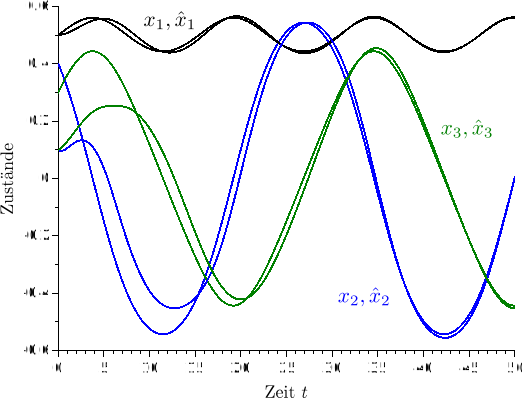
\includegraphics[width=0.8\textwidth]{Kreisel_HG}
\par\end{centering}
\caption{Simulation der Kreiselgleichungen und des zugehörigen High-Gain-Beobachters\label{fig:Kreisel-HG}}

\end{figure}

\begin{example}
\label{exa:wagen-pendel-hg1}Man betrachte das Wagen-Pendel-System
aus Abschnitt~\ref{subsec:Wagen-mit-Pendel}, allerdings ohne Eingang
($u=0$) und reibungsfrei ($d_{1}=0,$ $d_{2}=0$). Aus Gl.~(\ref{eq:modell-pendel-mit-wagen})
liest man das Vektorfeld 
\begin{equation}
f(x)=\left(\begin{array}{c}
x_{2}\\
\frac{m_{2}\sin x_{3}\left(g\cos x_{3}+\ell x_{4}^{2}\right)}{m_{1}+m_{2}\sin^{2}x_{3}}\\
x_{4}\\
-\frac{\sin x_{3}\left(g(m_{1}+m_{2})+\ell m_{2}x_{4}^{2}\cos x_{3}\right)}{\ell\left(m_{1}+m_{2}\sin^{2}x_{3}\right)}
\end{array}\right)\label{eq:hg-wagen-pendel-f0}
\end{equation}
ab. Als Ausgang verwenden wir zunächst die Position des Wagens, d.\,h.
$y_{1}=h_{1}(x)=x_{1}$ (siehe Abb.~\ref{fig:Wagen-mit-Pendel-Hig-Gain}).
Die Beobachtbarkeitsmatrix 
\begin{equation}
Q_{B}(x)=\left(\begin{array}{cccc}
1 & 0 & 0 & 0\\
0 & 1 & 0 & 0\\
0 & 0 & * & \frac{2\ell m_{2}x_{4}\sin x_{3}}{m_{1}+m_{2}\sin^{2}x_{3}}\\
0 & 0 & * & *
\end{array}\right)\label{eq:wageh-pendel-hg-Qb1}
\end{equation}
enthält in den letzten zwei Zeilen bzw. Spalten vergleichsweise komplizierte
Ausdrücke. Zur Überprüfung der Regularität der Beobachtbarkeitsmatrix
berechnen wir deren Determinante, für die man auch einen umfangreichen
Ausdruck erhält. Mit $\det Q_{B}(x)=(gm_{2}/m_{1})^{2}$ für $x_{3}=0$,
$x_{4}=0$ ist die Beobachtbarkeitsmatrix zumindest für kleine Auslenkungen
des Pendels und kleine Winkelgeschwindigkeiten regulär. Die Beobachterverstärkung
\[
k(\hat{x})=Q_{B}^{-1}(x)\cdot\left(\begin{array}{c}
a_{3}\\
a_{2}\\
a_{1}\\
a_{0}
\end{array}\right)=\left(\begin{array}{c}
a_{3}\\
a_{2}\\
*\\
*
\end{array}\right)
\]
nach Gl.~(\ref{eq:hg-beobachter-autonom-orig}) enthält in den letzten
zwei Komponenten ebenfalls sehr umfangreiche Ausdrücke, so dass auf
die vollständige Angabe verzichtet wird.
\end{example}
\begin{figure}
\begin{centering}
\resizebox{0.5\textwidth}{!}{\input{wagen_pendel_high_gain.pdftex_t}}
\par\end{centering}
\caption{Wagen mit Pendel\label{fig:Wagen-mit-Pendel-Hig-Gain}}
\end{figure}

\begin{example}
\label{exa:wagen-pendel-hg2}Wir betrachten erneut das Wagen-Pendel-System
aus Beispiel~\ref{exa:wagen-pendel-hg1}, verwenden jetzt aber die
horizontale Position der Last als Ausgang, d.\,h. $y_{2}=h_{2}(x)=x_{1}+\ell\sin x_{3}$
(vgl. Abb.~\ref{fig:Wagen-mit-Pendel-Hig-Gain}). Die zugehörige
Beobachtbarkeitsmatrix hat die Form 
\[
Q_{B}(x)=\left(\begin{array}{cccc}
1 & 0 & \ell\cos x_{3} & 0\\
0 & 1 & -\ell x_{4}\sin x_{3} & \ell\cos x_{3}\\
0 & 0 & * & -\frac{2\ell m_{1}x_{4}\sin x_{3}}{m_{1}+m_{2}\sin^{2}x_{3}}\\
0 & 0 & * & *
\end{array}\right).
\]
Mit $\det Q_{B}(x)=g^{2}$ für $x_{3}=0$, $x_{4}=0$ ist die Beobachtbarkeitsmatrix
auch mit diesem Ausgang für kleine Auslenkungen und kleine Winkelgeschwindigkeiten
regulär. Damit kann man den Beobachter~(\ref{eq:hg-beobachter-autonom-orig})
berechnen, erhält aber wiederum umfangreiche Ausdrücke.
\end{example}

Für die Konvergenzanalyse betrachten wir das System~(\ref{eq:hg-system-autonom})
und den Beobachter~(\ref{eq:hg-beobachter-autonom-trans}) in den
transformierten Koordinaten. Genügt die in der Fehlerdifferentialgleichung~(\ref{eq:hg-fehlerdyn})
auftretende Nichtlinearität~$\alpha$ einer Lipschitz-Bedingung\index{Lipschitz-Bedingung}
\begin{equation}
\forall\xi,\hat{\xi}:\quad\left\Vert \alpha(\xi)-\alpha(\hat{\xi})\right\Vert \leq\rho\left\Vert \xi-\hat{\xi}\right\Vert \label{eq:hg-lipschitz-bedingung}
\end{equation}
mit der Lipschitz-Konstanten $\rho>0$, dann kann über die Wahl der
Beobachterverstärkung~$l$ durch den linearen Teil $A-lc^{T}$ die
Konvergenz des Beobachters gesichert werden. Der folgende Satz trifft
eine globale Konvergenzaussage:
\begin{theorem}
\label{thm:hg-konvergenz-autonom}Gegeben sei System~(\ref{eq:hg-system-autonom})
zusammen mit dem Beobachter~(\ref{eq:hg-beobachter-autonom-orig}).
Das Vektorfeld~$f$ sei auf $\mathcal{M}=\R^{n}$ definiert und vollständig.
Die Beobachtbarkeitsabbildung~$q$ sei ein globaler Diffeomorphismus.
Außerdem genüge die Nichtlinearität~$\alpha$ der globalen Lipschitz-Bedingung~(\ref{eq:hg-lipschitz-bedingung}).
Dann existiert ein Vektor $l\in\R^{n}$ derart, dass 
\begin{equation}
\lim_{t\to\infty}\left\Vert \hat{x}(t)-x(t)\right\Vert =0\label{eq:hg-konvergenz}
\end{equation}
für alle Anfangswerte $x(0),\hat{x}(0)\in\mathcal{M}$ gilt.
\end{theorem}

Die Beweise in~\cite{gauthier92,ciccarella93,dalla-mora1997} basieren
auf sehr speziellen Eigenwertvorgaben. In späteren Arbeiten entfällt
diese Einschränkung. Der folgende Beweis beruht auf~\cite{roebenack2012ssd,roebenack2016sac}:\nocite{derbel2016sac}
\begin{svmultproof2}
Laut Annahme ist die Beobachtbarkeitsabbildung ein globaler Diffeomorphismus.
Wir führen daher die Konvergenzanalyse in den transformierten Koordinaten
durch und zeigen, dass die Ruhelage $\tilde{\xi}=0$ der Fehlerdifferentialgleichung~(\ref{eq:hg-fehlerdyn})
global asymptotisch stabil ist. Definiert man 
\begin{equation}
\Delta\alpha(\tilde{\xi},t):=\alpha(\xi)-\alpha(\hat{\xi}),\label{eq:hg-delta-alpha}
\end{equation}
dann lässt sich die Fehlerdifferentialgleichung~(\ref{eq:hg-fehlerdyn})
als Verknüpfung eines linearen zeitinvarianten Systems mit der Übertragungsfunktion
\[
G(s)=\left(sI-\left(A-lc^{T}\right)\right)^{-1}b=\frac{1}{\CP(s)}\left(\begin{array}{c}
1\\
s+a_{n-1}\\
s^{2}+a_{n-1}s+a_{n-2}\\
\vdots
\end{array}\right)
\]
und der zeitvarianten Nichtlinearität~(\ref{eq:hg-delta-alpha})
darstellen (vgl. Abb.~\ref{fig:Fehlerdynamik-High-Gain}). Wir gehen
davon aus, dass~(\ref{eq:hg-cp}) als Hurwitz-Polynom vorgegeben
wurde. Damit besitzt das lineare Teilsystem eine endliche Verstärkung,
d.\,h. $\|G\|_{\infty}<\infty$.
\begin{figure}
\begin{centering}
\resizebox{0.82\textwidth}{!}{\input{high-gain-nf1.pdftex_t}}
\par\end{centering}
\caption{Struktur der Fehlerdynamik~(\ref{eq:hg-fehlerdyn}) des High-Gain-Beobachters~(\ref{eq:hg-beobachter-autonom-trans})\label{fig:Fehlerdynamik-High-Gain}}
\end{figure}

Führt man bei der Beobachterverstärkung $l^{\epsilon}=(a_{n-1}/\epsilon,\ldots,a_{0}/\epsilon^{n})^{T}$
einen Skalierungsfaktor $\epsilon\in(0,1]$ ein, so erhält man das
in~$\epsilon$ parametrierte charakteristische Polynom
\begin{equation}
\begin{array}{lrl}
\CP^{\epsilon}(s) & := & \det(sI-A+l^{\epsilon}c^{T})\\
 & = & \frac{a_{0}}{\epsilon^{n}}+\frac{a_{1}}{\epsilon^{n-1}}s+\cdots+\frac{a_{n-1}}{\epsilon}s^{n-1}+s^{n}\\
 & = & \left(s-\frac{s_{1}}{\epsilon}\right)\cdots\left(s-\frac{s_{n}}{\epsilon}\right).
\end{array}\label{eq:hg-cp-epsilon}
\end{equation}
Für $\epsilon\to0$ entspricht diese Skalierung einer Streckung der
Eigenwerte nach links. Die zugehörige Übertragungsfunktion hat dann
die Form
\[
G^{\epsilon}(s)=\left(sI-\left(A-l^{\epsilon}c^{T}\right)\right)^{-1}b=\frac{1}{\CP^{\epsilon}(s)}\left(\begin{array}{c}
1\\
s+a_{n-1}\epsilon^{-1}\\
s^{2}+a_{n-1}\epsilon^{-1}s+a_{n-2}\epsilon^{-2}\\
\vdots
\end{array}\right).
\]
Für den Frequenzgang der $i$-ten Komponente gilt
\[
\begin{array}{ccl}
G_{i}^{\epsilon}(j\omega) & = & \frac{(j\omega)^{i-1}+\frac{a_{n-1}}{\epsilon}(j\omega)^{i-2}+\cdots+\frac{a_{n-i+1}}{\epsilon^{i-1}}}{\left(j\omega-\frac{s_{1}}{\epsilon}\right)\cdots\left(j\omega-\frac{s_{n}}{\epsilon}\right)}\\
 & = & \frac{(j\omega\epsilon)^{i-1}+a_{n-1}(j\omega\epsilon)^{i-2}+\cdots+a_{n-i+1}}{\left(j\omega\epsilon-s_{1}\right)\cdots\left(j\omega\epsilon-s_{n}\right)}\epsilon^{n-i+1}\\
 & = & \frac{(j\tilde{\omega})^{i-1}+a_{n-1}(j\tilde{\omega})^{i-2}+\cdots+a_{n-i+1}}{\left(j\tilde{\omega}-s_{1}\right)\cdots\left(j\tilde{\omega}-s_{n}\right)}\epsilon^{n-i+1}\\
 & = & G_{i}(j\tilde{\omega})\epsilon^{n-i+1}
\end{array}
\]
mit $\tilde{\omega}=\omega\epsilon$. Daraus folgt unmittelbar $\|G_{i}^{\epsilon}\|_{\infty}=\|G_{i}\|_{\infty}\epsilon^{n-i+1}\to0$
für $\epsilon\to0$. Somit lassen sich der Parameter~$\epsilon$
und damit die zugehörige Beobachterverstärkung~$l^{\epsilon}$ immer
so wählen, dass $\|G^{\epsilon}\|_{\infty}<1/\rho$. Mit einer derartigen
Wahl der Beobachterverstärkung im linearen Teilsystem ist die Gesamtverstärkung
des offenen Kreises kleiner als Eins. Nach dem Satz über die kleine
Kreisverstärkung ist die Ruhelage $\tilde{\xi}=0$ global asymptotisch
stabil, so dass die Konvergenz~(\ref{eq:hg-konvergenz}) gesichert
ist (siehe Anhang~\ref{sec:Stabilitaet-im-geschlossenen-Regelkreis}).
\end{svmultproof2}

\begin{remark}
Für die korrekte Festlegung der Beobachterverstärkung~$l$ ist die
Kenntnis der Lipschitz-Konstanten~$\rho$ aus Ungl.~(\ref{eq:hg-lipschitz-bedingung})
erforderlich. Die exakte Bestimmung der Lipschitz-Konstanten ist in
der Regel aufwendig. Alternativ könnte man versuchen, über Intervallarithmetik
eine Abschätzung der Lipschitz-Konstanten zu erhalten. Praktisch gibt
man zunächst Eigenwerte $s_{1},\ldots,s_{n}$ für ein stabiles charakteristisches
Polynom~(\ref{eq:hg-cp}) vor. Dann geht man zum charakteristischen
Polynom~(\ref{eq:hg-cp-epsilon}) mit $\epsilon=1$ über und verkleinert
$\epsilon>0$ solange, bis der Boebachter konvergiert. 
\end{remark}

\subsection{Beobachtbarkeit und Beobachterentwurf für eingangsabhängige Systeme\label{subsec:Beobachterentwurf-mit-eingang}}

Im Folgenden wird das in Abschnitt~\ref{subsec:Beobachtbarkeit-autonom}
zunächst für autonome Systeme eingeführte Konzept der Beobachtbarkeit
auf eingangsabhängige Systeme übertragen, um anschließend auch für
diese Systeme den Beobachter aus Abschnitt~\ref{subsec:Beobachterentwurf-autonom}
verwenden zu können.

Für die Beobachtbarkeitsanalyse betrachten wir das System~(\ref{eq:hg-system-nicht-affin})
auf dem Zeit\-inter\-vall $[0,T]$ mit $T>0$. Das Eingangssignal
$u(\cdot)$ sei auf diesem Zeit\-inter\-vall (mindestens) stückweise
stetig. Dann besitzt das System für hinreichend kleine $T>0$ ein
allgemeine Lösung, die wir in leichter Modifikation der bisherigen
Notation mit $\varphi_{t}^{u}$ bezeichnen (vgl. Abschnitt~\ref{sec:Vektorfelder-und-Fluesse}).
Zwei Zustände $p,\bar{p}\in\mathcal{M}$ heißen \emph{nicht unterscheidbar
bezüglich eines (gegebenen) Eingangssignals} $u(\cdot)$\index{Nichtunterscheidbarkeit!bezüglich eines Eingangssignals},
wenn die zugehörigen Verläufe der Ausgänge übereinstimmen, d.\,h.
\[
\forall t\in[0,T]:\quad h(\varphi_{t}^{u}(p))=h(\varphi_{t}^{u}(\bar{p})).
\]
Mit dem Begriff der Unterscheidbarkeit lassen sich in Analogie zu
Abschnitt~\ref{subsec:Beobachtbarkeit-autonom} auch lokale und globale
Beobachtbarkeit für eingangsabhängige Systeme definieren. Das folgende
Beispiel zeigt, dass bei einem nichtlinearen System die Möglichkeit,
den Zustand aus dem Verlauf des Ausgangs und seinen Zeitableitungen
zu rekonstruieren, vom konkreten Eingangssignal abhängen kann:

\begin{example}
\label{exa:Minisystem-nicht-glm-beob}Gegeben sei das System
\begin{equation}
\begin{array}{lcl}
\dot{x}_{1} & = & -x_{1}+x_{2}(1+u)\\
\dot{x}_{2} & = & x_{2}\\
y & = & x_{1}.
\end{array}\label{eq:Minisystem-nicht-glm-beob}
\end{equation}
Für $u\neq-1$ erhält man den Zustand~$x$ aus dem Ausgang~$y$
und seiner ersten Zeitableitung:
\[
\left.\begin{array}{lcl}
y & = & x_{1}\\
\dot{y} & = & -x_{1}+x_{2}(1+u)
\end{array}\right\} \quad\Longrightarrow\quad\begin{array}{lcl}
x_{1} & = & y,\\
x_{2} & = & \frac{y+\dot{y}}{1+u}.
\end{array}
\]
Für $u\equiv-1$ wirkt sich dagegen der Zustand~$x_{2}$ nicht auf
den Ausgang aus. In diesem Fall sind alle Anfangszustände, die in
der ersten Komponente übereinstimmen, nicht unterscheidbar.
\end{example}

Das Beispiel verdeutlicht, dass es sinnvoll sein kann, die Beobachtbarkeit
eines eingangsabhängigen Systems derart zu definieren, dass diese
Eigenschaft unabhängig vom gewählten Eingangssignal ist. Wir nennen
ein System~(\ref{eq:hg-system-eingangsaffin}) \emph{gleichmäßig
lokal} bzw. \emph{global beobachtbar}, wenn es für alle zulässigen
Eingangssignale $u(\cdot)$ lokal bzw. global beobachtbar ist. 

Gegeben sei ein eingangsaffines System
\begin{equation}
\dot{x}=f(x)+g(x)u,\quad y=h(x)\label{eq:hg-system-eingangsaffin}
\end{equation}
mit den Vektorfeldern $f,g:\mathcal{M}\to\R^{n}$ und dem Skalarfeld
$h:\mathcal{M}\to\R$. Die Felder seien hinreichend glatt. Erfüllt
der autonome Teil~(\ref{eq:hg-system-autonom}) von System~(\ref{eq:hg-system-eingangsaffin})
die Bedingungen von Lemma~\ref{lem:Beobachtbarkeit-hinreichende-Bedingung},
so ist eine Beurteilung der gleichmäßigen lokalen Beobachtbarkeit
anhand der Beobachtbarkeitsnormalform\index{Beobachtbarkeitsnormalform}\index{Normalform!Beobachtbarkeits-}
möglich~\cite{gauthier81,gauthier92}:
\begin{theorem}
\label{thm:hg-Beobachtbarkeit-nicht-autonom}Man betrachte das System~(\ref{eq:hg-system-eingangsaffin})
im Punkt $p\in\mathcal{M}$. Es gelte $\rank\,Q_{B}(p)=n$. Das System
ist genau dann gleichmäßig lokal beobachtbar im Punkt~$p$, wenn
es zustands\-äquivalent zur Form 
\begin{equation}
\begin{array}{lcl}
\dot{\xi}_{1} & = & \xi_{2}+\beta_{1}(\xi_{1})u\\
\dot{\xi}_{2} & = & \xi_{3}+\beta_{2}(\xi_{1},\xi_{2})u\\
 & \vdots\\
\dot{\xi}_{n-1} & = & \xi_{n}+\beta_{n-1}(\xi_{1},\xi_{2},\ldots,\xi_{n-1})u\\
\dot{\xi}_{n} & = & \alpha(\xi)+\beta_{n}(\xi_{1},\xi_{2},\ldots,\xi_{n-1},\xi_{n})u\\
y & = & \xi_{1}
\end{array}\label{eq:Beobachtbarkeits-NF-nicht-autonom}
\end{equation}
ist.
\end{theorem}
\begin{svmultproof2}
Es gelte $\rank\,Q_{B}(p)=n$. Dann ist die in Gl.~(\ref{eq:Beobachtbarkeitsabbildung})
definierte Beobachtbarkeitsabbildung $\xi=q(x)$ ein lokaler Diffeomorphismus,
der das System~(\ref{eq:hg-system-eingangsaffin}) in die Beobachtbarkeitsnormalform\index{Beobachtbarkeitsnormalform}\index{Normalform!Beobachtbarkeits-}
\begin{equation}
\begin{array}{lcl}
\dot{\xi}_{1} & = & \xi_{2}+\beta_{1}(\xi)u\\
\dot{\xi}_{2} & = & \xi_{3}+\beta_{2}(\xi)u\\
 & \vdots\\
\dot{\xi}_{n-1} & = & \xi_{n}+\beta_{n-1}(\xi)u\\
\dot{\xi}_{n} & = & \alpha(\xi)+\beta_{n}(\xi)u\\
y & = & \xi_{1}
\end{array}\label{eq:Beobachtbarkeits-NF-nicht-autonom-allgemein}
\end{equation}
mit $\alpha(\xi):=L_{f}^{n}h(q^{-1}(\xi))$ und 
\begin{equation}
\beta_{i}(\xi):=L_{g}L_{f}^{i-1}h(q^{-1}(\xi))\quad\text{für}\quad i=1,\ldots,n\label{eq:beobachtbarkeits-NF-beta-i}
\end{equation}
überführt (vgl. Beweis von Satz~\ref{thm:hg-beobachtbarkeitsnormalform}).
Für die nachfolgenden Untersuchungen betrachten wir zwei Instanzen
des Systems~(\ref{eq:Beobachtbarkeits-NF-nicht-autonom-allgemein}),
nämlich eine mit dem Zustand~$\xi$ und dem Anfangswert $\xi(0)$
und eine weitere Instanz mit dem Zustand~$\bar{\xi}$ und dem Anfangswert
$\bar{\xi}(0)$. Beide Instanzen werden mit dem gleichen Eingangssignal~$u$
beaufschlagt.

\notwendig\ Wir zeigen die Notwendigkeit der Form~(\ref{eq:Beobachtbarkeits-NF-nicht-autonom})
indirekt. Wir nehmen also an, dass das System~(\ref{eq:Beobachtbarkeits-NF-nicht-autonom-allgemein})
nicht der speziellen Struktur~(\ref{eq:Beobachtbarkeits-NF-nicht-autonom})
genügt. Sei $i_{0}<n$ die kleinste Zahl, so dass eine Zahl $j_{0}>i_{0}$
mit $\partial\beta_{i_{0}}/\partial\xi_{j_{0}}\not\equiv0$ existiert.
(Das bedeutet, dass $\beta_{i_{0}}(\xi)$ nicht nur von $\xi_{1},\ldots,\xi_{i_{0}}$,
sondern auch von $\xi_{j_{0}}$ abhängt.) Die Anfangswerte $\xi(0)\neq\bar{\xi}(0)$
beider Systeminstanzen seien so gewählt, dass sie in den ersten~$i_{0}$
Komponenten übereinstimmen, d.\,h. $\xi_{i}(0)=\bar{\xi}_{i}(0)$
für $i=1,\ldots,i_{0}$. Wegen $\partial\beta_{i_{0}}/\partial\xi_{j_{0}}\not\equiv0$
lassen sich zusätzlich die $j_{0}$-ten Komponenten $\xi_{j_{0}}(0)\neq\bar{\xi}_{j_{o}}(0)$
beider Anfangswerte so wählen, dass $\beta_{i_{0}}(\xi(0))-\beta_{i_{0}}(\bar{\xi}(0))\neq0$
gilt. Die Rückführung 
\begin{equation}
u=-\frac{\xi_{i_{0}+1}-\bar{\xi}_{i_{0}+1}}{\beta_{i_{0}}(\xi)-\beta_{i_{0}}(\bar{\xi})}\label{eq:beweis-struktur-nicht-autonom-u}
\end{equation}
ist damit zumindest für ein gewisses Zeitintervall $[0,T]$ bei hinreichend
kleiner Endzeit $T>0$ definiert. Die Abweichung in der $i_{0}$-ten
Differentialgleichung beider Instanzen verschwindet unter Wirkung
des Eingangssignals~(\ref{eq:beweis-struktur-nicht-autonom-u}) identisch:
\[
\dot{\xi}_{i_{0}}-\dot{\bar{\xi}}_{i_{0}}=\xi_{i_{0}+1}+\bar{\xi}_{i_{0}+1}+\left(\beta_{i_{0}}(\xi)-\beta_{i_{0}}(\bar{\xi})\right)u\equiv0.
\]
Dann stimmen die Zeitverläufe in den ersten $i_{0}$ Komponenten von
$\xi,\bar{\xi}$ auf dem Intervall $[0,T]$ überein und führen somit
unabhängig von den Anfangswerten der letzten $n-i_{0}$ Komponenten
zu dem gleichen Ausgangsverlauf. Damit sind alle Anfangswerte $\xi(0),\bar{\xi}(0)$,
die in den ersten $i_{0}$ Komponenten übereinstimmen, für den Eingangsverlauf~(\ref{eq:beweis-struktur-nicht-autonom-u})
nicht unterscheidbar. Das System ist also nicht gleichmäßig lokal
beobachtbar.

\hinreichend\ Das transformierte System~(\ref{eq:Beobachtbarkeits-NF-nicht-autonom-allgemein})
besitze die Struktur~(\ref{eq:Beobachtbarkeits-NF-nicht-autonom}).
Für beide Instanzen des Systems~(\ref{eq:Beobachtbarkeits-NF-nicht-autonom})
betrachten wir beliebige Verläufe von dem Ausgang $y(t)=\xi_{1}(t)=\bar{\xi}_{1}(t)$
und dem Eingang $u(t)$ für alle $t\in[0,T]$ mit $T>0$. Durch Einsetzen
in die erste Differentialgleichung von~(\ref{eq:Beobachtbarkeits-NF-nicht-autonom})
erhält man übereinstimmende Verläufe $\xi_{2}(t)=\bar{\xi}_{2}(t)$,
aus der zweiten Differentialgleichung folgt $\xi_{3}(t)=\bar{\xi}_{3}(t)$.
Dieses Verfahren setzt man bis zur vorletzen Differentialgleichung
fort, aus der man $\xi_{n}(t)=\bar{\xi}_{n}(t)$ für alle $t\in[0,T]$
erhält. Damit gilt $\xi(t)=\bar{\xi}(t)$ für alle $t\in[0,T]$, so
dass auch die Anfangswerte beider Systeminstanzen übereinstimmen:
$\xi(0)=\bar{\xi}(0)$. Für einen vorgegebenen Ausgangsverlauf ist
unabhängig vom konkreten Eingangsverlauf der Anfangswert eindeutig
festgelegt. Das System~(\ref{eq:Beobachtbarkeits-NF-nicht-autonom})
ist daher gleichmäßig beobachtbar.
\end{svmultproof2}

Die Argumentation im hinreichenden Teil des Beweises lässt unmittelbar
eine Verallgemeinerung auf nicht eingangsaffine Systeme mit ggf. vektorwertigem
Eingang zu:
\begin{corollary}
\label{cor:Beobachtbarkeit-nicht-affin-MISO}Gegeben sei ein System
\[
\dot{x}=f(x)+\tilde{g}(x,u),\quad y=h(x)
\]
mit hinreichend glatten Feldern $f:\mathcal{M}\to\R^{n}$, $\tilde{g}:\mathcal{M}\times\mathcal{U}\to\R^{n}$,
$h:\mathcal{M}\to\R$ und $\mathcal{U}\subseteq\R^{m}$. Für das zugeordnete
autonome System~(\ref{eq:hg-system-autonom}) gelte $\rank\,Q_{B}(p)=n$
in einem Punkt $p\in\mathcal{M}$. Ist das System in einer Umgebung
von~$p$ zustands\-äquivalent zur Form
\begin{equation}
\begin{array}{lcl}
\dot{\xi}_{1} & = & \xi_{2}+\tilde{\beta}_{1}(\xi_{1},u)\\
\dot{\xi}_{2} & = & \xi_{3}+\tilde{\beta}_{2}(\xi_{1},\xi_{2},u)\\
 & \vdots\\
\dot{\xi}_{n-1} & = & \xi_{n}+\tilde{\beta}_{n-1}(\xi_{1},\xi_{2},\ldots,\xi_{n-1},u)\\
\dot{\xi}_{n} & = & \alpha(\xi)+\tilde{\beta}_{n}(\xi_{1},\xi_{2},\ldots,\xi_{n-1},\xi_{n},u)\\
y & = & \xi_{1},
\end{array}\label{eq:Beobachtbarkeits-NF-nicht-affin}
\end{equation}
dann ist es im Punkt~$p$ gleichmäßig lokal beobachtbar.
\end{corollary}

Für einige eingangsaffine Beispielssysteme wird die Existenz der speziellen
Form~(\ref{eq:Beobachtbarkeits-NF-nicht-autonom}) untersucht:

\begin{example}
\label{exa:Minisystem-nicht-glm-Beobachtbarkeits-NF}Das System~(\ref{eq:Minisystem-nicht-glm-beob})
aus Beispiel~\ref{exa:Minisystem-nicht-glm-beob} besitzt eine lineare
Beobachtbarkeitsabbildung~(\ref{eq:Beobachtbarkeitsabbildung}) und
folglich eine konstante Beobachtbarkeitsmatrix~(\ref{eq:Beobachtbarkeitsmatrix}):
\[
\xi=q(x)=\left(\begin{array}{c}
x_{1}\\
-x_{1}+x_{2}
\end{array}\right),\quad Q_{B}(x)=q^{\prime}(x)=\left(\begin{array}{rc}
1 & 0\\
-1 & 1
\end{array}\right).
\]
Damit ist die Umkehrtransformation $x=q^{-1}(\xi)$ auch linear: $x_{1}=\xi_{1}$,
$x_{2}=\xi_{1}+\xi_{2}$. Das transformierte System lautet
\[
\begin{array}{lcl}
\dot{\xi} & = & \frac{\d}{\d t}q(x)\\
 & = & q^{\prime}(x)\cdot\dot{x}\\
 & = & Q_{B}(x)\left(f(x)+g(x)u\right)\\
 & = & \left.\left(\begin{array}{rc}
1 & 0\\
-1 & 1
\end{array}\right)\left(\begin{array}{c}
-x_{1}+x_{2}(1+u)\\
x_{2}
\end{array}\right)\right|_{x=q^{-1}(\xi)}\\
 & = & \left(\begin{array}{c}
\xi_{2}+(\xi_{1}+\xi_{2})u\\
\xi_{1}-(\xi_{1}+\xi_{2})u
\end{array}\right).
\end{array}
\]
Das System liegt damit in der Form~(\ref{eq:Beobachtbarkeits-NF-nicht-autonom-allgemein})
mit $\beta_{1}(\xi)=\xi_{1}+\xi_{2}$ und $\beta_{2}(\xi)=-(\xi_{1}+\xi_{2})$
vor. Da $\beta_{1}(\xi)$ auch von~$\xi_{2}$ abhängt, ist die Struktur~(\ref{eq:Beobachtbarkeits-NF-nicht-autonom})
nicht gegeben. Das System ist also in Übereinstimmung mit den Betrachtungen
aus Beispiel~\ref{exa:Minisystem-nicht-glm-beob} nicht gleichmäßig
lokal beobachtbar.
\end{example}

\begin{example}
\label{exa:hg-mathematisches-Pendel-Drehmoment}Das inverse mathematische
Pendel aus Beispiel~\ref{exa:hg-inverses-pendel} mit der Ausgangsgröße
aus Beispiel~\ref{exa:hg-mathematisches-Pendel-autonom} lässt sich
durch das Zustandsraummodell
\begin{equation}
\begin{array}{lcl}
\dot{x}_{1} & = & x_{2}\\
\dot{x}_{2} & = & \kappa_{1}\sin x_{1}+\kappa_{2}u\\
y & = & x_{2}
\end{array}\label{eq:hg-math-pendel-drehmoment}
\end{equation}
beschreiben. Aus der Beobachtbarkeitsabbildung~(\ref{eq:hg-math-pendel-q})
erhält man Hin- und Rücktransformation 
\[
\begin{array}{lcl}
\xi_{1} & = & x_{2}\\
\xi_{2} & = & \kappa_{1}\sin x_{1}
\end{array}\qquad\text{und}\qquad\begin{array}{lcl}
x_{1} & = & \arcsin\frac{\xi_{2}}{\kappa_{1}}\\
x_{2} & = & \xi_{1}
\end{array}
\]
in die Beobachtbarkeitsnormalform~(\ref{eq:Beobachtbarkeits-NF-nicht-autonom-allgemein}).
Daraus ergibt sich das transformierte System 
\begin{equation}
\begin{array}{lcl}
\dot{\xi}_{1} & = & \xi_{2}+\kappa_{2}u\\
\dot{\xi}_{2} & = & \kappa_{1}\xi_{1}\sqrt{1-\frac{\xi_{2}^{2}}{\kappa_{1}^{2}}}
\end{array}\label{eq:hg-math-pendel-transformiert}
\end{equation}
mit $\beta_{1}(\xi)=\kappa_{2}$ und $\beta_{2}(\xi)=0$. Dabei hängt
$\beta_{1}(\xi)$ nicht von~$\xi_{2}$ ab, so dass das System~(\ref{eq:hg-math-pendel-transformiert})
in de Form~(\ref{eq:Beobachtbarkeits-NF-nicht-autonom}) vorliegt
und für $|x_{1}|<\pi/2$ nach Satz~\ref{thm:hg-Beobachtbarkeit-nicht-autonom}
gleichmäßig lokal beobachtbar ist. Mit der Beobachterverstärkung~(\ref{eq:math-pendel-autonom-beobachterverstaerkung-x})
erhält man für das erregte System~(\ref{eq:hg-math-pendel-drehmoment})
den Beobachter
\[
\left(\begin{array}{l}
\dot{\hat{x}}_{1}\\
\dot{\hat{x}}_{2}
\end{array}\right)=\left(\begin{array}{c}
\hat{x}_{2}\\
\kappa_{1}\sin\hat{x}_{1}+\kappa_{2}u
\end{array}\right)+\left(\begin{array}{c}
\frac{a_{0}}{\kappa_{1}\cos\hat{x}_{1}}\\
a_{1}
\end{array}\right)\left(y-\hat{x}_{2}\right)
\]
mit den Koeffizienten $a_{0},a_{1}>0$.
\end{example}

\begin{example}
\label{exa:Synchronmaschine-HG}In~\cite{mukhopadhyay1972} wird
eine Synchronmaschine\index{Synchronmaschine} modelliert und durch
die Zustandsgleichungen 
\begin{equation}
\begin{array}{lcl}
\dot{x}_{1} & = & x_{2}\\
\dot{x}_{2} & = & B_{1}-A_{1}x_{2}-A_{2}x_{3}\sin x_{1}-\tfrac{1}{2}B_{2}\sin(2x_{1})\\
\dot{x}_{3} & = & u-D_{1}x_{3}+D_{2}\cos x_{1}\\
y & = & x_{1}
\end{array}\label{eq:synchronmotor}
\end{equation}
beschrieben. Dabei bezeichnet~$x_{1}$ den Polradwinkel, also den
Winkel zwischen dem Polrad und dem Drehfeld. Der Polradwinkel fungiert
zugleich als Ausgangsgröße, welche aus dem mit einen Winkelencoder
erfassten Drehwinkel berechnet wird. Fernen seien $x_{2}$ die zugehörige
Winkelgeschwindigkeit (relativ zum rotierenden Bezugssystem), $x_{3}$
die Flussverkettung der Erregerwicklung und $u$ der Eingang.

Das Modell~(\ref{eq:synchronmotor}) wird häufig zu Vergleichszwecken
beim nichtlinearen Beobachterentwurf verwendet~\cite{keller86diss,birk88,adjallah94,roebenack2003buch,roebenack2005habil,adamy2014,franke2016pamm}.
Die Beobachtbarkeitsmatrix 
\begin{equation}
Q_{B}(x)=\left(\begin{array}{ccc}
1 & 0 & 0\\
0 & 1 & 0\\
-A_{2}x_{2}\cos x_{1}-B_{2}\cos(2x_{1}) & -A_{1} & -A_{2}\sin x_{1}
\end{array}\right)\label{eq:synchronmotor-beobachtbarkeitsmatrix}
\end{equation}
ist für $x_{1}\neq\pi i$ mit $i\in\mathbb{Z}$ regulär, so dass der
zugehörige autonome Systemteil, den man für $u=0$ erhält, in diesem
Bereich lokal beobachtbar ist. Zur Untersuchung der gleichmäßigen
Beobachtbarkeit betrachten wir die Struktur des aus~(\ref{eq:synchronmotor})
resultierenden Eingangsvektorfeldes $g(x)=\tfrac{\partial}{\partial x_{3}}$
in den transformierten Koordinaten:
\[
Q_{B}(x)\cdot g(x)=\left(\begin{array}{c}
0\\
0\\
-A_{2}\sin x_{1}
\end{array}\right).
\]
Mit $\beta_{1}(\cdot)=0$ und $\beta_{2}(\cdot)=0$ ist die Strukturbedingung~(\ref{eq:Beobachtbarkeits-NF-nicht-autonom})
erfüllt, so dass das System~(\ref{eq:synchronmotor}) im o.\,g.
Bereich gleichmäßig lokal beobachtbar ist. Die Beobachterverstärkung
hat die Form
\[
k(\hat{x})=Q_{B}^{-1}(\hat{x})\left(\begin{array}{c}
a_{2}\\
a_{1}\\
a_{0}
\end{array}\right)=\left(\begin{array}{c}
a_{2}\\
a_{1}\\
-\frac{a_{0}+a_{1}A_{1}+a_{2}A_{2}\hat{x}_{3}\cos\hat{x}_{1}+a_{2}B_{2}\cos(2\hat{x}_{1})}{A_{2}\sin\hat{x}_{1}}
\end{array}\right)
\]
mit den Koeffizienten $a_{0},a_{1},a_{2}>0$. Simulationsuntersuchungen
des Beobachters sind in~\cite{roebenack2003buch} beschrieben.
\end{example}

Bei komplizierteren Systemen lässt sich die Beobachtbarkeitsnormalform~(\ref{eq:Beobachtbarkeits-NF-nicht-autonom-allgemein})
in der Regel nicht explizit angeben. In diesen Fällen ist Satz~\ref{thm:hg-Beobachtbarkeit-nicht-autonom}
zur Überprüfung der gleichmäßigen Beobachtbarkeit nicht geeignet.
Mit folgendem Satz ist die Überprüfung der Struktur~(\ref{eq:Beobachtbarkeits-NF-nicht-autonom})
auch in Originalkoordinaten möglich~\cite[Lemma~2]{jo2002}:
\begin{theorem}
\label{thm:hg-Beobachtbarkeit-nicht-autonom2}Man betrachte das System~(\ref{eq:hg-system-eingangsaffin})
im Punkt $p\in\mathcal{M}$. Es gelte $\rank\,Q_{B}(p)=n$. Das System
ist genau dann gleichmäßig lokal beobachtbar im Punkt~$p$, wenn
\begin{equation}
\d L_{g}L_{f}^{i}h\in\spann\{\d h,\d L_{f}h,\ldots,\d L_{f}^{i}h\}\quad\text{für}\quad i=0,\ldots,n-2\label{eq:beob-nicht-autonom-grad-x}
\end{equation}
in einer Umgebung von~$p$ gilt.
\end{theorem}
\begin{svmultproof2}
Es gelte $\rank\,Q_{B}(p)=n$. Dann ist die in Gl.~(\ref{eq:Beobachtbarkeitsabbildung})
definierte Beobachtbarkeitsabbildung $\xi=q(x)$ ein lokaler Diffeomorphismus,
der das System~(\ref{eq:hg-system-eingangsaffin}) in die Beobachtbarkeitsnormalform~(\ref{eq:Beobachtbarkeits-NF-nicht-autonom-allgemein})
überführt. Die in Gl.~(\ref{eq:Beobachtbarkeits-NF-nicht-autonom})
angegebenen funkionalen Abhängigkeiten in den Komponenten~$\beta_{i}$
des (transformierten) Eingangsvektorfeldes lassen sich über lineare
Abhängigkeiten ausdrücken:
\begin{equation}
\begin{array}{lclcl}
\beta_{1}(\xi_{1}) & \quad\Longleftrightarrow\quad & \d\beta_{1} & \in & \spann\{\d\xi_{1}\}\\
\beta_{2}(\xi_{1},\xi_{2}) & \quad\Longleftrightarrow\quad & \d\beta_{2} & \in & \spann\{\d\xi_{1},\d\xi_{2}\}\\
 & \vdots\\
\beta_{n-1}(\xi_{1},\xi_{2},\ldots,\xi_{n-1}) & \quad\Longleftrightarrow\quad & \d\beta_{n-1} & \in & \spann\{\d\xi_{1},\d\xi_{2},\ldots,\d\xi_{n-1}\}.
\end{array}\label{eq:beob-nicht-autonom-grad-z}
\end{equation}
Aus $\xi_{i}=L_{f}^{i-1}h(x)$ ergibt sich $\d\xi_{i}=\d L_{f}^{i-1}h(x)$
für $i=1,\ldots,n$. Mit~(\ref{eq:beobachtbarkeits-NF-beta-i}) wertet
Gl.~(\ref{eq:beob-nicht-autonom-grad-x}) die in Gl.~(\ref{eq:beob-nicht-autonom-grad-z})
beschriebenen Abhängigkeiten in den Originalkoordinaten aus. Die Anwendung
von Satz~\ref{thm:hg-Beobachtbarkeit-nicht-autonom} liefert den
Bezug zur gleichmäßigen lokalen Beobachtbarkeit.
\end{svmultproof2}

\begin{example}
Wir ergänzen das in Beispiel~\ref{exa:wagen-pendel-hg1} betrachtete
Wagen-Pendel-System um das Eingangsvektorfeld
\[
g(x)=\left(\begin{array}{c}
0\\
\frac{1}{m_{1}+m_{2}\sin^{2}x_{3}}\\
0\\
-\frac{\cos x_{3}}{l(m_{1}+m_{2}\sin^{2}x_{3})}
\end{array}\right)
\]
aus Abschnitt~\ref{subsec:Wagen-mit-Pendel}. Mit dem Vektorfeld~$f$
aus Gl.~(\ref{eq:hg-wagen-pendel-f0}) und dem Ausgang $y=h(x)=x_{1}$
berechnet man die Lie-Ableitungen 
\[
\begin{array}{lcl}
L_{g}h(x) & = & 0\\
L_{g}L_{f}h(x) & = & \frac{1}{m_{1}+m_{2}\sin^{2}x_{3}}\\
L_{g}L_{f}^{2}h(x) & = & -2\frac{m_{2}x_{4}\sin x_{3}\cos x_{3}}{(m_{1}+m_{2}\sin^{2}x_{3})^{2}},
\end{array}
\]
deren Gradienten die folgende Struktur aufweisen:
\[
\begin{array}{lcc}
\d L_{g}h & = & (\,0\,,\,0\,,\,0\,,\,0\,)\phantom{.}\\
\d L_{g}L_{f}h & = & (\,0\,,\,0\,,\,*\,,\,0\,)\phantom{.}\\
\d L_{g}L_{f}^{2}h & = & (\,0\,,\,0\,,\,*\,,\,*\,).
\end{array}
\]
Aus den ersten zwei Zeilen der Beobachtbarkeitsmatrix~(\ref{eq:wageh-pendel-hg-Qb1})
liest man $\d\xi_{1}=\d h=\d x_{1}$ und $\d\xi_{2}=\d L_{f}h=\d x_{2}$
ab. Damit ist Bedingung~(\ref{eq:beob-nicht-autonom-grad-x}) für
$i=1$ nicht erfüllt, d.\,h. aus $\d L_{g}L_{f}h\in\spann\{\d x_{3}\}$
folgt $\d L_{g}L_{f}h\notin\spann\{\d h,\d L_{f}h\}=\spann\{\d x_{1},\d x_{2}\}$.
Das System ist also nicht gleichmäßig beobachtbar.
\end{example}

\begin{remark}
Der beschriebene Zugang zum Entwurf von High-Gain-Beobachtern lässt
sich für Mehrgrößensysteme verallgemeinern~\cite{dalla-mora2000}.
Gleichzeitig zur Schätzung des Zustands ist grundsätzlich auch eine
Parameterschätzung mittels Adaption möglich~\cite{bullinger1997cdc,besancon2004}.
Erhält man für die Beobachtbarkeitsmatrix umfangreiche Ausdrücke,
so bietet sich die Berechnung mit algorithmischem Differenzieren an~\cite{rr2000nolta,roebenack2005dsmc,roebenack2005habil}.
Ist die Beobachtbarkeitsrangbedingung~(\ref{eq:Beobachtbarkeitsrangbedingung})
erfüllt, aber die Beobachtbarkeitsmatrix~(\ref{eq:Beobachtbarkeitsmatrix})
singulär, dann empfiehlt sich der Entwurf eines Einbettungsbeobachters~\cite{gauthier91}.\index{Beobachter!Einbettungs-}
\end{remark}

\section{Beobachterentwurf auf Basis der Eingangs-Ausgangs-Normalform\label{sec:High-Gain-Entwurf-Eingangs-Ausgangs-Normalform}}

\subsection{Struktur des Beobachters}

Die gleichmäßig lokale Beobachtbarkeit eines eingangsaffinen Systems~(\ref{eq:hg-system-eingangsaffin})
setzt die Zustandsäquivalenz zur Form~(\ref{eq:Beobachtbarkeits-NF-nicht-autonom})
voraus. Dabei unterliegen mit Ausnahme der letzten Komponente alle
anderen Komponenten des transformierten Eingangsvektorfeldes hinsichtlich
der zulässigen Abhängigkeiten bestimmten Strukturbedingungen. Bei
einem System mit wohldefiniertem relativen Grad würde der Eingang
nur in der letzten Differentialgleichungen des ersten Teilsystems
der Eingangs-Ausgangs-Normalform in Erscheinung treten. Die vorangegangenen
Komponenten des transformierten Eingangsvektorfeldes sind dabei identisch
Null, so dass das erste Teilsystem (unter Beachtung der zusätzlichen
Abhängigkeiten vom zweiten Teilsystem) der Strukturbedingung~(\ref{eq:Beobachtbarkeits-NF-nicht-autonom})
genügt. Dieser Abschnitt behandelt die in~\cite{jo2000b,roebenack2004at,roebenack2007ndst}
vorgestellten Entwurfsverfahren, bei denen der in Abschnitt~\ref{sec:High-Gain-Entwurf-Beobachtbarkeitsnormalform}
beschriebene Beobachterentwurf von der Beobachtbarkeitsnormalform
auf die Eingangs-Ausgang- bzw. Byrnes-Isidori-Normalform übertragen
wird.

Das eingangsaffine System~(\ref{eq:hg-system-eingangsaffin}) habe
einen wohldefinierten relativen Grad $r<n$. Dann kann das System
mit einer Zustandstransformation 
\begin{equation}
\left(\begin{array}{c}
\xi\\
\eta
\end{array}\right)=\Phi(x)\label{eq:hg-EA-Phi}
\end{equation}
 in die Eingangs-Ausgangs-Normalform
\begin{equation}
\left.\begin{array}{lcl}
\dot{\xi}_{1} & = & \xi_{2}\\
 & \vdots\\
\dot{\xi}_{r-1} & = & \xi_{r}\\
\dot{\xi}_{r} & = & \alpha(\xi,\eta)+\beta(\xi,\eta)u\\
\dot{\eta}_{1} & = & q_{1}(\xi,\eta)+d_{1}(\xi,\eta)u\\
 & \vdots\\
\dot{\eta}_{n-r} & = & q_{n-r}(\xi,\eta)+d_{n-r}(\xi,\eta)u\\
y & = & \xi_{1}
\end{array}\right\} \quad\begin{array}{rcl}
\dot{\xi} & = & A\xi+b(\alpha(\xi,\eta)+\beta(\xi,\eta)u)\\
\dot{\eta} & = & q(\xi,\eta)+d(\xi,\eta)u\\
y & = & c^{T}\xi
\end{array}\label{eq:hg-EA-NF}
\end{equation}
transformiert werden (siehe Abschnitt~\ref{subsec:Byrnes-Isidori-Normalform}).
Das erste Teilsystem besitzt weitgehend die Struktur der Beobachtbarkeitsnormalform~(\ref{eq:Beobachtbarkeits-NF-autonom}),
d.\,h., dass die Nichtlinearitäten, die hier zusätzlich über den
Eingang beeinflusst werden, nur in der letzten Zeile auftreten. Daher
wird der Beobachter für das erste Teilsystem auch in der Form analog
zu Gl.~(\ref{eq:hg-beobachter-autonom-trans}) angesetzt. Der Korrekturterm
wirkt nicht direkt auf das zweite Teilsystem. Insgesamt erhält man
dabei den Ansatz 
\begin{equation}
\begin{array}{rcl}
\dot{\hat{\xi}} & = & A\hat{\xi}+b(\alpha(\hat{\xi},\hat{\eta})+\beta(\hat{\xi},\hat{\eta})u)+l\cdot(y-\hat{\xi}_{1})\\
\dot{\hat{\eta}} & = & q(\hat{\xi},\hat{\eta})+d(\hat{\xi},\hat{\eta})u
\end{array}\label{eq:hg-EA-NF-Beobachter}
\end{equation}
mit der konstanten Beobachterverstärkung $l\in\R^{r}$. Der Beobachtungsfehler
$\tilde{\xi}=\xi-\hat{\xi}$ und $\tilde{\eta}=\eta-\hat{\eta}$ genügt
dem Differentialgleichungssystem
\begin{equation}
\begin{array}{lcl}
\dot{\tilde{\xi}} & = & \left(A-lc^{T}\right)\tilde{\xi}+b\left[\alpha(\xi,\eta)+\beta(\xi,\eta)u-\alpha(\hat{\xi},\hat{\eta})-\beta(\hat{\xi},\hat{\eta})u\right]\\
\dot{\tilde{\eta}} & = & q(\xi,\eta)+d(\xi,\eta)u-q(\hat{\xi},\hat{\eta})-d(\hat{\xi},\hat{\eta})u.
\end{array}\label{eq:hg-EA-fehler-dgl}
\end{equation}
In Anlehnung an Gl.~(\ref{eq:hg-cp}) erhält man mit $l=(a_{r-1},\ldots,a_{0})^{T}$
das charakteristische Polynom 
\begin{equation}
\begin{array}{crl}
\CP(s) & := & \det(sI-(A-lc^{T}))\\
 & = & a_{0}+a_{1}s+\cdots+a_{r-1}s^{r-1}+s^{r}\\
 & = & (s-s_{1})\cdots(s-s_{r}).
\end{array}\label{eq:hg-cp-EA-NF}
\end{equation}
Man würde Eigenwerte $s_{1},\ldots,s_{r}$, die hinreichend weit links
in der komplexen Ebene liegen, vorgeben und daraus die Koeffizienten
$p_{0},\ldots,p_{r-1}$ des charakteristischen Polynoms~(\ref{eq:hg-cp-EA-NF})
berechnen. Mit 
\[
\left(\begin{array}{c}
\dot{\hat{\xi}}\\
\dot{\hat{\eta}}
\end{array}\right)=\frac{\d}{\d t}\Phi(\hat{x})=\Phi^{\prime}(\hat{x})\cdot\dot{\hat{x}}
\]
lässt sich der Beobachter~(\ref{eq:hg-EA-NF-Beobachter}) in den
Originalkoordinaten angeben:
\begin{equation}
\begin{array}{lll}
\dot{\hat{x}} & = & \left(\Phi^{\prime}(\hat{x})\right)^{-1}\cdot\left(\begin{array}{c}
\dot{\hat{\xi}}\\
\dot{\hat{\eta}}
\end{array}\right)\\
 & = & \left(\Phi^{\prime}(\hat{x})\right)^{-1}\cdot\left(\begin{array}{c}
A\hat{\xi}+b(\alpha(\hat{\xi},\hat{\eta})+\beta(\hat{\xi},\hat{\eta})u)+l\cdot(y-\hat{\xi}_{1})\\
q(\hat{\xi},\hat{\eta})+d(\hat{\xi},\hat{\eta})u
\end{array}\right)\\
 & = & f(\hat{x})+g(\hat{x})u+\left(\Phi^{\prime}(\hat{x})\right)^{-1}\cdot\left(\begin{array}{c}
l\\
0
\end{array}\right)\cdot(y-h(\hat{x}))\\
 & =: & f(\hat{x})+g(\hat{x})u+k(\hat{x})\cdot(y-h(\hat{x})).
\end{array}\label{eq:hg-EA-Beobachter-x}
\end{equation}
Damit erhält man eine vom Beobachterzustand abhängige Beobachterverstärkung
$k:\mathcal{M}\to\R^{n}$. Anwendungen dieses Beobachteransatzes sind
beispielsweise in~\cite{gao2010,mahmud2011,ide2013,koester2015}
zu finden.

\subsection{Berechnung der Beobachterverstärkung auf Basis der Byrnes-Isidori-Normalform}

Eine besondere Situation liegt vor, wenn die Koordinatentransformation~(\ref{eq:hg-EA-Phi})
in die Eingangs-Ausgangs-Normalform~(\ref{eq:hg-EA-NF}) so gewählt
wird, dass $d\equiv0$ gilt. In diesem Fall geht~(\ref{eq:hg-EA-NF})
in die Byrnes-Isidori-Normalform 
\begin{equation}
\begin{array}{rcl}
\dot{\xi} & = & A\xi+b(\alpha(\xi,\eta)+\beta(\xi,\eta)u)\\
\dot{\eta} & = & q(\xi,\eta)\\
y & = & c^{T}\xi
\end{array}\label{eq:hg-BI-NF}
\end{equation}
über. Dabei vereinfacht sich die Fehlerdynamik~(\ref{eq:hg-EA-fehler-dgl})
zu 
\begin{equation}
\begin{array}{lcl}
\dot{\tilde{\xi}} & = & \left(A-lc^{T}\right)\tilde{\xi}+b\left[\alpha(\xi,\eta)+\beta(\xi,\eta)u-\alpha(\hat{\xi},\hat{\eta})-\beta(\hat{\xi},\hat{\eta})u\right]\\
\dot{\tilde{\eta}} & = & q(\xi,\eta)-q(\hat{\xi},\hat{\eta}).
\end{array}\label{eq:hg-BI-NF-fehler-dgl}
\end{equation}
Der nachfolgende Satz gibt globale Konvergenzbedingungen an. Schwächere
Existenzbedingungen, die allerdings einen umfangreicheren Beweis mit
sich bringen, sind in~\cite{jo2000b} zu finden.

\begin{theorem}
\label{thm:hg-konvergenz-BI-BF}System~(\ref{eq:hg-system-eingangsaffin})
habe einen gleichmäßigen relativen Grad~$r$ auf $\mathcal{M}=\R^{n}$.
Zusätzlich sei die Transformation~(\ref{eq:hg-EA-Phi}) in die Byrnes-Isidori-Normalform~(\ref{eq:uio-BI-NF})
ein globaler Diffeomorphismus. Die Nichtlinearitäten des ersten Teilsystems
genügen einer globalen Lipschitz-Bedingung\index{Lipschitz-Bedingung}
\begin{equation}
\forall\xi,\hat{\xi},\eta,\hat{\eta},u:\quad\left\Vert \alpha(\xi,\eta)+\beta(\xi,\eta)u-\alpha(\hat{\xi},\hat{\eta})-\beta(\hat{\xi},\hat{\eta})u\right\Vert \leq\rho\left\Vert \xi-\hat{\xi}\right\Vert \label{eq:hg-BI-NF-Lipschitz}
\end{equation}
gleichmäßig in $\eta,\hat{\eta},u$. Existieren eine global positiv
definite Funktion~$V_{2}$ und Funktionen $\gamma_{1},\gamma_{2}$
der Klasse~$\mathcal{K}_{\infty}$ derart, dass die Zeit\-ableitung
von~$V_{2}(\tilde{\eta})$ entlang der Fehlerdynamik~(\ref{eq:hg-BI-NF-fehler-dgl})
der Bedingung 
\begin{equation}
\forall\tilde{\xi},\tilde{\eta}:\quad\dot{V}_{2}\leq-\gamma_{1}(\|\tilde{\eta}\|)+\gamma_{2}(\|\tilde{\xi}\|)\label{eq:hg-BI-NF-dV}
\end{equation}
genügt, dann existiert eine Beobachterverstärkung $l\in\R^{r}$ derart,
dass der Beobachter~(\ref{eq:hg-EA-Beobachter-x}) global konvergiert.
\end{theorem}
\begin{proofsketch}Mit der Bedingung~(\ref{eq:hg-BI-NF-Lipschitz})
lässt sich die globale asympotitsche Stabilität der Ruhelage $\tilde{\xi}=0$
des ersten Teilsystems der Fehler\-dynamik~(\ref{eq:hg-BI-NF-fehler-dgl})
analog zu Satz~\ref{thm:hg-konvergenz-autonom} zeigen. Nach Gl.~(\ref{eq:hg-BI-NF-dV})
ist das zweite Teilsystem der Fehlerdynamik~(\ref{eq:hg-BI-NF-fehler-dgl})
eingangs-zustands-stabil bezüglich~$\tilde{\xi}$. Aufgrund der Kaskaden\-struktur
ist die Ruhelage $(\tilde{\xi},\tilde{\eta})=(0,0)$ der Fehlerdynamik~(\ref{eq:hg-BI-NF-fehler-dgl})
global asymptotisch stabil.\end{proofsketch}

Die Bedingung~(\ref{eq:hg-BI-NF-dV}), welche die Eingangs-Zustands-Stabilität
des zweiten Teilsystems der Fehlerdynamik sichert, gewährleistet die
Ermittelbarkeit des Gesamtsystems~\cite{amicucci1998,sontag97oss}.
Hinsichtlich des zweiten Teilsystems der Regelstrecke~(\ref{eq:hg-BI-NF})
entspricht die Bedingung~(\ref{eq:hg-BI-NF-dV}) einer inkrementellen
Eingangs-Zustands-Stabilität~\cite{Angeli2002}.

\begin{example}
\label{exa:isidori434-HG-BI-NF}Das folgende Beispielsystem entstammt
aus~\cite[S.~{167}]{isidori3}:
\begin{equation}
\begin{array}{lcl}
\dot{x}_{1} & = & x_{3}-x_{2}^{3}\\
\dot{x}_{2} & = & -x_{2}-x_{3}^{2}u\\
\dot{x}_{3} & = & -x_{3}+x_{1}^{2}+u\\
y & = & x_{1}.
\end{array}\label{eq:isidori434-system}
\end{equation}
Mit $L_{g}h(x)=0$ und $L_{g}L_{f}h(x)=1+3x_{2}^{2}x_{3}^{2}>0$ ist
der relative Grad $r=2$ im gesamten Zustandsraum $\mathcal{M}=\R^{3}$
wohldefiniert. Zur Transformation in die Byrnes-Isidori-Normalform
ist eine Funktion~$\phi_{3}$ gesucht, welche die partielle Differentialgleichung
\[
L_{g}\phi_{3}(x)=-x_{3}^{2}\frac{\partial\phi_{3}(x)}{\partial x_{2}}+\frac{\partial\phi_{3}(x)}{\partial x_{3}}=0
\]
erfüllt. Eine mögliche Wahl ist $\phi_{3}(x)=x_{2}+x_{3}^{3}/3$.
Die zugehörige Transformation~(\ref{eq:hg-EA-Phi}) lautet 
\[
\Phi(x)=\left(\begin{array}{c}
h(x)\\
L_{f}h(x)\\
\phi_{3}(x)
\end{array}\right)=\left(\begin{array}{c}
x_{1}\\
x_{3}-x_{2}^{3}\\
x_{2}+\frac{1}{3}x_{3}^{3}
\end{array}\right).
\]
Aus der Jacobimatrix
\begin{equation}
\Phi^{\prime}(x)=\left(\begin{array}{ccc}
1 & 0 & 0\\
0 & -3x_{2}^{2} & 1\\
0 & 1 & x_{3}^{2}
\end{array}\right)\label{eq:isidori434-dPhi}
\end{equation}
ergibt sich die auf ganz~$\mathcal{M}$ definierte Beobachterverstärkung
\begin{equation}
k(\hat{x})=\left(\Phi^{\prime}(\hat{x})\right)^{-1}\left(\begin{array}{c}
a_{1}\\
a_{0}\\
0
\end{array}\right)=\left(\begin{array}{c}
a_{1}\\
-\frac{a_{0}\hat{x}_{3}^{2}}{1+3\hat{x}_{2}^{2}\hat{x}_{3}^{2}}\\
\frac{a_{0}}{1+3\hat{x}_{2}^{2}\hat{x}_{3}^{2}}
\end{array}\right)\label{eq:isidori434-k-BINF}
\end{equation}
mit den Koeffizienten $a_{0},a_{1}>0$.
\end{example}

\begin{example}
\label{exa:Wagen-Pendel-HG-BINF}Wir betrachten das gedämpfte Wagen-Pendel-System
aus Abschnitt~\ref{subsec:Wagen-mit-Pendel}. Für den Ausgang $y=x_{1}$
(Position der Last) besitzt das System den relativen Grad $r=2$ (siehe
Beispiel~\ref{exa:Wagen-Pendel-partielle-Linearisierung}). In Beispiel~\ref{exa:Wagen-Pendel-System-BINF}
wurde für das partiell linearisierte Systeme die Transformation
\[
\Phi(x)=\left(\begin{array}{c}
x_{1}\\
x_{2}\\
x_{3}\\
x_{4}+\frac{1}{l}x_{2}\cos x_{3}
\end{array}\right)\quad\text{mit}\quad\Phi^{\prime}(x)=\left(\begin{array}{cccc}
1 & 0 & 0 & 0\\
0 & 1 & 0 & 0\\
0 & 0 & 1 & 0\\
0 & -\frac{1}{l}\cos x_{3} & \frac{x_{2}}{l}\cos x_{3} & 1
\end{array}\right)
\]
in die Byrnes-Isidori-Normalform berechnet. Diese Transformation überführt
auch das nicht partiell linearisierte Originalsystem in die Byrnes-Isidori-Normalform.
Das ist daran zu erkennen, dass die letzten $n-r=2$ Komponenten des
transformierten Eingangsvektorfelds verschwinden:
\[
\Phi_{*}g(x)=\Phi^{\prime}(x)g(x)=\left(\begin{array}{c}
0\\
\frac{1}{m_{1}+m_{2}\sin^{2}x_{3}}\\
0\\
0
\end{array}\right).
\]
Aus Gl.~(\ref{eq:hg-EA-Beobachter-x}) ergibt sich die Beobachterverstärkung
\[
k(\hat{x})=\left(\Phi^{\prime}(\hat{x})\right)^{-1}\cdot\left(\begin{array}{c}
a_{1}\\
a_{0}\\
\hline 0\\
0
\end{array}\right)=\left(\begin{array}{c}
a_{1}\\
a_{0}\\
0\\
-\frac{a_{0}}{l}\cos\hat{x}_{3}
\end{array}\right)
\]
mit $a_{0},a_{1}>0$. Es ist zu erwarten, dass der Beobachter hinsichtlich
des zweites Teilsystems, welches maßgeblich vom rotatorischen Teil
bestimmt wird, aufgrund der Dämpfung (Reibung) konvergiert. 
\end{example}

\subsection{Berechnung der Beobachterverstärkung mit der Moore-Penrose-Inversen}

Die bei der Transformation in die Eingangs-Ausgangs-Normalform~(\ref{eq:hg-EA-NF})
bestehenden Freiheitsgrade für die Koordinaten des zweiten Teilsystems
lassen sich auch nutzen, um eine möglichst einfache Berechnungsvorschrift
für die in Gl.~(\ref{eq:hg-EA-Beobachter-x}) definierte Beobachterverstärkung~$k$
zu erhalten~\cite{roebenack2004at,roebenack2007ndst}. In diesen
Zusammenhang fällt auf, dass die Jacobimatrix~$\Phi^{\prime}$ der
Transformation~(\ref{eq:hg-EA-Phi}) in den ersten $r$ Zeilen mit
der Beobachtbarkeitsmatrix~$Q_{B}$ übereinstimmt. Diese $r$ Zeilen
definieren die \emph{reduzierte} \emph{Beobachtbarkeitsmatrix}\index{Beobachtbarkeitsmatrix!reduzierte}
\[
Q(x)=\left(\begin{array}{c}
\d h(x)\\
\d L_{f}h(x)\\
\vdots\\
\d L_{f}^{r-1}h(x)
\end{array}\right).
\]
Bei einem im Punkt $p\in\mathcal{M}$ wohldefinierten relativen Grad
sind die Zeilen dieser Matrix linear unabhängig (Lemma~\ref{lem:Lin-Unabh-Kovektoren}).
Die verbleibenden $n-r$ Zeilen von~$\Phi^{\prime}$ fassen wir in
einer $(n-r)\times n$-Matrix
\[
R(x)=\left(\begin{array}{c}
\d\phi_{r+1}(x)\\
\vdots\\
\d\phi_{n}(x)
\end{array}\right)
\]
zusammen. Die Zeilen der Matrix~$Q$ bestehen nach Konstruktion aus
exakten Kovektorfeldern. Nach Korollar~\ref{cor:ergaenzung-einer-kodistribution-integrierbar}
lassen sich die Zeilen der Matrix~$R$ so wählen, dass die $n\times n$-Gesamtmatrix
\begin{equation}
\Phi^{\prime}(x)=\left(\begin{array}{c}
Q(x)\\
R(x)
\end{array}\right)\label{eq:hg-EA-QR-Jac}
\end{equation}
regulär ist und zusätzlich die Zeilen von~$Q$ und~$R$ senkrecht
aufeinander stehen, z.\,B. es gilt 
\begin{equation}
R(x)\cdot Q^{T}(x)=0\label{eq:hg-EA-QR-orth}
\end{equation}
für alle~$x$ aus einer Umgebung von~$p$. Wegen dieser Orthogonalität
kann man die Inverse der Jacobimatrix~(\ref{eq:hg-EA-QR-Jac}) blockweise
über die \index{Moore-Penrose-Inverse}\emph{Moore-Penrose-Inversen}~$Q^{+}$
und~$R^{+}$ der Matrizen~$Q$ und~$R$ beschreiben~\cite{boullion71,rao71,ben-israel}:
\[
\left(\begin{array}{c}
Q(x)\\
R(x)
\end{array}\right)^{-1}=\left(Q^{+}(x)\,|\,R^{+}(x)\right).
\]
Dann vereinfacht sich die Beobachterverstärkung zu
\begin{equation}
k(x)=\left(\Phi^{\prime}(x)\right)^{-1}\cdot\left(\begin{array}{c}
l\\
0
\end{array}\right)=\left(Q^{+}(x)\,|\,R^{+}(x)\right)\cdot\left(\begin{array}{c}
l\\
0
\end{array}\right)=Q^{+}(x)\cdot l,\label{eq:hg-k-Moore-Penrose-Inverse}
\end{equation}
so dass für deren Berechnung die Matrix~$R$ nicht explizit benötigt
wird. Da die reduzierte Beobachtbarkeitsmatrix~$Q$ vollen Zeilenrang
besitzt, lässt sich deren Moore-Penrose-Inverse folgendermaßen berechnen:
\[
Q^{+}=Q^{T}\left(QQ^{T}\right)^{-1}.
\]

\begin{example}
\label{exa:isidori434-HG-MPPI}Das System~(\ref{eq:isidori434-system})
aus Beispiel~\ref{exa:isidori434-HG-BI-NF} hat den relativen Grad
$r=2$. Daraus ergibt sich die reduzierte Beobachtbarkeitsmatrix 
\[
Q(x)=\left(\begin{array}{c}
\d h(x)\\
\d L_{f}h(x)
\end{array}\right)=\left(\begin{array}{ccc}
1 & 0 & 0\\
0 & -3x_{2}^{2} & 1
\end{array}\right),
\]
vgl. Gl.~(\ref{eq:isidori434-dPhi}). Nach Gl.~(\ref{eq:hg-k-Moore-Penrose-Inverse})
erhält man die Beobachterverstärkung 
\begin{equation}
k(\hat{x})=Q^{+}(x)\cdot\left(\begin{array}{c}
a_{1}\\
a_{0}
\end{array}\right)=\left(\begin{array}{c}
a_{1}\\
-\frac{3a_{0}\hat{x}_{2}^{2}}{1+9\hat{x}_{2}^{4}}\\
\frac{a_{0}}{1+9\hat{x}_{2}^{4}}
\end{array}\right),\label{eq:isidori434-k-MPPI}
\end{equation}
Dieses Ergebnis wird von der mit \textsc{Maxima} durchgeführten Kontrollrechnung
bestätigt:

\begin{maxima}\noindent
%%%%%%%%%%%%%%%
%%% INPUT:
\begin{minipage}[t]{8ex}\color{red}\bf
\begin{verbatim}
(%i5) 
\end{verbatim}
\end{minipage}
\begin{minipage}[t]{\textwidth}\color{blue}
\begin{verbatim}
f:[x3-x2^3,-x2,-x3+x1^2]$
g:[0,-x3^2,1]$
h:x1$
x:[x1,x2,x3]$
\end{verbatim}
\end{minipage}

\smallskip

\noindent
%%%%%%%%%%%%%%%
%%% INPUT:
\begin{minipage}[t]{8ex}\color{red}\bf
\begin{verbatim}
(%i8) 
\end{verbatim}
\end{minipage}
\begin{minipage}[t]{\textwidth}\color{blue}
\begin{verbatim}
r:RelativeDegree(f,g,h,x)$
qred:makelist(LieScalar(f,h,x,i),i,0,r-1)$
Q:jacobian(qred,x);
\end{verbatim}
\end{minipage}
%%% OUTPUT:

\noindent
$\displaystyle
\parbox{8ex}{$\color{labelcolor}\mathrm{\tt (\%o8) }\quad $}
\begin{pmatrix}1 & 0 & 0\cr 0 & -3\cdot {{\mathit{x2}}^{2}} & 1\end{pmatrix}\mbox{}
$
%%%%%%%%%%%%%%%


\noindent
%%%%%%%%%%%%%%%
%%% INPUT:
\begin{minipage}[t]{8ex}\color{red}\bf
\begin{verbatim}
(%i10) 
\end{verbatim}
\end{minipage}
\begin{minipage}[t]{\textwidth}\color{blue}
\begin{verbatim}
l:makelist(a[i],i,r-1,0,-1)$
k:moore_penrose_pseudoinverse(Q).l;
\end{verbatim}
\end{minipage}
%%% OUTPUT:

\noindent
$\displaystyle
\parbox{8ex}{$\color{labelcolor}\mathrm{\tt (\%o10) }\quad $}
\begin{pmatrix}{{a}_{1}}\cr -\frac{3\cdot {{a}_{0}}\cdot {{\mathit{x2}}^{2}}}{9\cdot {{\mathit{x2}}^{4}}+1}\cr \frac{{{a}_{0}}}{9\cdot {{\mathit{x2}}^{4}}+1}\end{pmatrix}\mbox{}
$
%%%%%%%%%%%%%%%
\end{maxima}

Kombiniert man den Beobachter~(\ref{eq:hg-EA-Beobachter-x}) mit
einem Regelgesetz entsprechend Abschnitt~\ref{sec:E-A-Linearisierung-affin},
dann ist sowohl mit der Beobachterverstärkung~(\ref{eq:isidori434-k-BINF})
aus Beispiel~\ref{exa:isidori434-HG-BI-NF} als auch mit der Beobachterverstärkung~(\ref{eq:isidori434-k-MPPI})
eine Stabilisierung der Ruhelage $x=0$ möglich~\cite{roebenack2004at}.
\end{example}

\begin{example}
\label{exa:Wagen-Pendel-HG-MPPI}Für das gedämpfte Wagen-Pendel-System
aus Beispiel~\ref{exa:Wagen-Pendel-HG-BINF} erhält man aus der reduzierten
Beobachtbarkeitsmatrix
\[
Q(x)=\left(\begin{array}{cccc}
1 & 0 & 0 & 0\\
0 & 1 & 0 & 0
\end{array}\right)
\]
die sehr einfache (nämlich konstante) Beobachterverstärkung
\[
k(\hat{x})=\left(\begin{array}{c}
a_{1}\\
a_{0}\\
0\\
0
\end{array}\right)
\]
mit $a_{0},a_{1}>0$. Die dem translatorischen Teilsystem zugeordneten
Beobachterzustände $\hat{x}_{1},\hat{x}_{2}$ werden über diese Beobachterverstärkung
direkt beeinflusst. Die das rotatorische Teilsystem beschreibenden
Beobachterzustände $\hat{x}_{3},\hat{x}_{4}$ werden als Simulationsterm,
der vom ersten Teilsystem über~$\hat{x}_{2}$ angeregt wird, mitgeführt.
Unter Annahme einer geeigneten Dämpfung konvergiert der Beobachter.
\end{example}

\section{Beobachterentwurf bei unbekanntem Eingang}

Bei den bisher behandelten Beobachtern wurde davon ausgegangen, dass
man bei einem System mit Eingang diesen auch messen kann. Schätzt
ein Beobachter den Systemzustand bei Messung des Ausgangs~$y$, aber
ohne Kenntnis des (vorhandenen) Systemeingangs~$u$ (vgl. Abb.~\ref{fig:uio-struktur}),
so spricht man von einem \emph{Beobachter mit unbekanntem Eingang}\index{Beobachter!mit unbekanntem Eingang}
(engl. \emph{unkown input observer}, kurz \emph{UIO}) oder einem \emph{starken
Beobachter} (engl. \emph{strong observer}). Diese Art des Beobachters
setzt man ein, wenn die messtechnische Erfassung der Eingangsgröße
sehr aufwendig bzw. nicht möglich ist. Die Existenzbedingungen und
der Beobachterentwurf werden für lineare Systeme in einem kürzlich
erschienenen Übersichtsbeitrag beschrieben~\cite{lunze2017at}. Dieser
Abschnitt befasst sich mit der Berechnung eines starken Beobachters
für eine spezielle Klasse nicht\-linearer Systeme~\cite{moreno2000UnknownInput}.

\begin{figure}
\begin{centering}
\resizebox{0.55\textwidth}{!}{\input{uio.pdftex_t}}
\par\end{centering}
\caption{Zustandsbeobachtung bei unbekanntem Eingang\label{fig:uio-struktur}}

\end{figure}

Man betrachtet das eingangsaffine Eingrößensystem~(\ref{eq:hg-system-eingangsaffin}).
Bei wohldefiniertem relativen Grad~$r$ existiert immer eine Transformation~(\ref{eq:hg-EA-Phi}),
die das System in die Byrnes-Isidori-Normalform~(\ref{eq:hg-BI-NF})
überführt. Im Fall $r=1$ gilt $\xi=\xi_{1}=y$, d.\,h. der eindimensionale
Zustand des ersten Teilsystems ist der Ausgang. Damit lässt sich die
Byrnes-Isidori-Normalform~(\ref{eq:hg-BI-NF}) auch folgendermaßen
angeben: 
\begin{equation}
\begin{array}{rcl}
\dot{y} & = & \alpha(y,\eta)+\beta(y,\eta)u\\
\dot{\eta} & = & q(y,\eta)
\end{array}\label{eq:uio-BI-NF}
\end{equation}
Der starke Beobachter 
\begin{equation}
\begin{array}{ccl}
\dot{\hat{\eta}} & = & q(y,\hat{\eta})\\
\hat{x} & = & \Phi^{-1}(y,\hat{\eta})
\end{array}\label{eq:uio-beobachter}
\end{equation}
besteht aus einer Kopie des zweiten Teilsystems von~(\ref{eq:uio-BI-NF}),
welches direkt vom gemessenen Ausgang~$y$ erregt wird. Da das zweite
Teilsystem bei $r=1$ die Dimension $n-1$ besitzt, handelt es sich
um einen reduzierten Beobachter\index{Beobachter!reduzierter}. Bemerkenswert
ist, dass beim Beobachter kein Einstellparameter (z.\,B. in Form
einer Beobachterverstärkung) auftritt. Mit der Rücktransformation~$\Phi^{-1}$
erhält man den Schätzwert des Zustands in den Originalkoordinaten.

Für die Untersuchung der Konvergenz des Beobachters ist lediglich
das zweite Teilsystem zu betrachten. Mit $\tilde{\eta}=\eta-\hat{\eta}$
erhält man die Fehlerdifferentialgleichung
\begin{equation}
\dot{\tilde{\eta}}=q(y,\eta)-q(y,\hat{\eta}),\label{eq:uio-fehler-dgl}
\end{equation}
deren Konvergenz der Gegenstand des folgenden Satzes ist:
\begin{theorem}
\label{thm:uio-konvergenz-global}System~(\ref{eq:hg-system-eingangsaffin})
habe einen gleichmäßigen relativen Grad $r=1$ auf $\mathcal{M}=\R^{n}$.
Zusätzlich sei die Transformation~(\ref{eq:hg-EA-Phi}) in die Byrnes-Isidori-Normalform~(\ref{eq:uio-BI-NF})
ein globaler Diffeomorphismus. Existieren eine global positiv definite
Funktion~$V$ und eine Funktion~$\gamma$ der Klasse~$\mathcal{K}_{\infty}$
derart, dass die Zeit\-ableitung von~$V(\tilde{\eta})$ entlang
der Fehlerdynamik~(\ref{eq:uio-fehler-dgl}) der Bedingung 
\begin{equation}
\forall\eta,\hat{\eta}:\quad\dot{V}(\eta,\hat{\eta})\leq-\gamma(\|\eta-\hat{\eta}\|)\label{eq:uio-dV}
\end{equation}
genügt, dann konvergiert der Beobachter~(\ref{eq:uio-beobachter})
global.
\end{theorem}
\begin{svmultproof2}
Bei gleichmäßigem relativen Grad und einer globalen Transformation
kann die Konvergenzuntersuchung in den Koordinaten der Bynres-Isidori-Normalform
erfolgen. Die Funktion~$V$ ist eine strenge Ljapunov-Funktion für
das Fehlersystem~(\ref{eq:uio-fehler-dgl}). Mit~(\ref{eq:uio-dV})
ist die Ruhelage $\tilde{\eta}=0$ von~(\ref{eq:uio-fehler-dgl})
global asymptotisch stabil (vgl. Anhang~\ref{sec:Stabilitaet-autonomer-Systeme}).
Damit konvergiert der Beobachter~(\ref{eq:uio-beobachter}) global.
\end{svmultproof2}

Die Funktion eines starken Beobachters wird an folgendem Beispiel
illustriert:
\begin{example}
Das Hodgkin-Huxley-Modell beschreibt das Aktionspotential eines Neurons~\cite{hodgkin1952}.
Das Aktionspotential ist eine Spannung~$U$, die zwischen dem Inneren
und dem Äußeren der Zelle abfällt. Die Zellmembran wirkt als Kondensator
mit dem Kapazitätsbelag $C=1\,\text{\ensuremath{\mu}F}/\text{cm}^{2}$.
Die Dynamik des Aktionspotentials lässt sich durch die Differentialgleichung
\begin{equation}
C\dot{U}=I-I_{\text{Na}}-I_{\text{K}}-I_{\text{L}}\label{eq:uio-hodgkin1}
\end{equation}
beschreiben. Dabei wird die Stromdichte in die Zelle (z.\,B. durch
äußere Erregung) mit~$I$ bezeichnet. Die Bewegung von \hbox{Natrium-}
bzw. Kalium\-ionen verursacht die Stromdichten~$I_{\text{Na}}$
bzw.~$I_{\text{K}}$. Zusätzlich enthält das Modell eine Leckstromdichte~$I_{\text{L}}$.
Die letztgenannten Stromdichten werden durch die Gleichungen
\begin{equation}
\begin{array}{lcl}
I_{\text{Na}} & = & g_{\text{Na}}m^{3}h\left(U-U_{\text{Na}}\right)\\
I_{\text{K}} & = & g_{\text{K}}n^{4}\left(U-U_{\text{K}}\right)\\
I_{\text{L}} & = & g_{\text{L}}\left(U-U_{\text{L}}\right)
\end{array}\label{eq:uio-hodgkin2}
\end{equation}
mit den flächenbezogenenen Leitwerten $g_{\text{Na}}=120\,\text{mS}/\text{cm}^{2}$,
$g_{\text{K}}=36\,\text{mS}/\text{cm}^{2}$, $g_{\text{L}}=0,3\,\text{mS}/\text{cm}^{2}$
und den Spannungen $U_{\text{Na}}=50\,\text{mV}$, $U_{\text{K}}=-77\,\text{mV}$,
$U_{\text{L}}=-54,4\,\text{mV}$ beschrieben. Die Durchlässigkeit
der Ionenkanäle wird durch die Zustände $m,h,n$ und das Markovmodell
\begin{equation}
\begin{array}{ccl}
\dot{m} & = & \alpha_{m}(U)\,(1-m)-\beta_{m}(U)\,m\\
\dot{h} & = & \alpha_{h}(U)\,(1-h)-\beta_{h}(U)\,h\\
\dot{n} & = & \alpha_{n}(U)\,(1-n)-\beta_{n}(U)\,n
\end{array}\label{eq:uio-hoghkin3}
\end{equation}
mit den Übergangsraten 
\begin{equation}
\begin{array}{lcl}
\alpha_{m}(U) & = & 0,1(U+40)/(1-\exp(-(U+40)/10)),\\
\beta_{m}(U) & = & 4\exp(-(U+65)/18),\\
\alpha_{h}(U) & = & 0,07\exp(-(U+65)/20),\\
\beta_{h}(U) & = & 1/(1+\exp(-(U+35)/10)),\\
\alpha_{n}(U) & = & 0,01(U+55)/(1-\exp(-(U+55)/10)),\\
\beta_{n}(U) & = & 0,125\exp(-(U+65)/80)
\end{array}\label{eq:uio-hodgkin4}
\end{equation}
modelliert. Die Spannung~$U$ ist dabei auf $\text{mV}$ normiert.
Das zu den Modellgleichungen~(\ref{eq:uio-hodgkin1}) und~(\ref{eq:uio-hodgkin2})
gehörende elektrische Ersatzschaltbild ist in Abb.~\ref{fig:hodgkin-huxley-netzwerk}
dargestellt.

\begin{figure}
\begin{centering}
\resizebox{0.5\textwidth}{!}{\input{hodgkin-huxley-modell.pdftex_t}}
\par\end{centering}
\caption{Ersatznetzwerk des Hodgkin-Huxley-Modells\label{fig:hodgkin-huxley-netzwerk}}

\end{figure}

Mit dem Ausgang $y=U$ liegt das durch Gln.~(\ref{eq:uio-hodgkin1})
bis~(\ref{eq:uio-hodgkin4}) beschriebene Modell bereits in der Byrnes-Isidori-Normalform
vor. Für die Simulation des Systems verwenden wir die Anfangswerte
$U(0)=-61,733\,\text{mV}$, $m(0)=0,0722$, $h(0)=0,4794$, $n(0)=0,3687$
und das Eingangssignal
\[
I(t)=\left\{ \begin{array}{rcl}
5 & \text{für} & 0\leq t\leq100\\
10 & \text{für} & t>100
\end{array}\right.
\]
mit der Zeit~$t$ in $\text{ms}$ und der Stromdichte~$I$ in $\text{\ensuremath{\mu}A}/\text{cm}^{2}$.
Zum Zeitpunkt $t=100$ wird die Zelle stimuliert. Der zugehörige Spannungsverlauf
ist in Abb.~\ref{fig:hodgkin-huxley-simulation} (oben) dargestellt.

Den Beobachter setzt man einfach als Kopie des Systems~(\ref{eq:uio-hoghkin3})
an, wobei man die Zustände $m,h,n$ in $\hat{m},\hat{h},\hat{n}$
umbenennt. Zur Überprüfung der Konvergenzbedingung~(\ref{eq:uio-dV})
setzen wir~$V$ als quadratische Form $V(\tilde{\eta})=\tfrac{1}{2}\sum_{i=1}^{3}\tilde{\eta}_{i}^{2}$
mit $\tilde{\eta}=(\tilde{m},\tilde{h},\tilde{n})^{T}$ an. Damit
ist~$V$ global positiv definit. Für die Zeitableitung von~$V$
entlang der sich aus~(\ref{eq:uio-hoghkin3}) ergebenden Fehlerdynamik
gilt 
\begin{equation}
\dot{V}=\sum_{i=1}^{3}\tilde{\eta}_{i}\dot{\tilde{\eta}}_{i}=-\sum_{i=1}^{3}\left(\alpha_{i}(U)+\beta_{i}U)\right)\tilde{\eta}_{i}^{2}\leq-\mu\|\tilde{\eta}\|^{2}\label{eq:uio-hodgkin-dV}
\end{equation}
mit $\mu:=\inf_{i,U}(\alpha_{i}(U)+\beta_{i}U))>0$, wobei die Funktionen~(\ref{eq:uio-hodgkin4})
entsprechend der Gleichungssnummer in~(\ref{eq:uio-hoghkin3}) notiert
wurden, d.\,h. $\alpha_{1}=\alpha_{m},\ldots,\beta_{3}=\beta_{n}$.
Mit~(\ref{eq:uio-hodgkin-dV}) ist Bedingung~(\ref{eq:uio-dV})
erfüllt, so dass der Beobachter global konvergiert. Für die Simulation
des Beobachter wird der Anfangsvektor $\hat{\eta}=0\in\R^{3}$ gewählt.
In Abb.~\ref{fig:hodgkin-huxley-simulation} (unten) ist zu sehen,
dass die Beobachtertrajektorien schnell gegen die Systemtrajektorien
konvergieren.

\begin{figure}
\begin{centering}
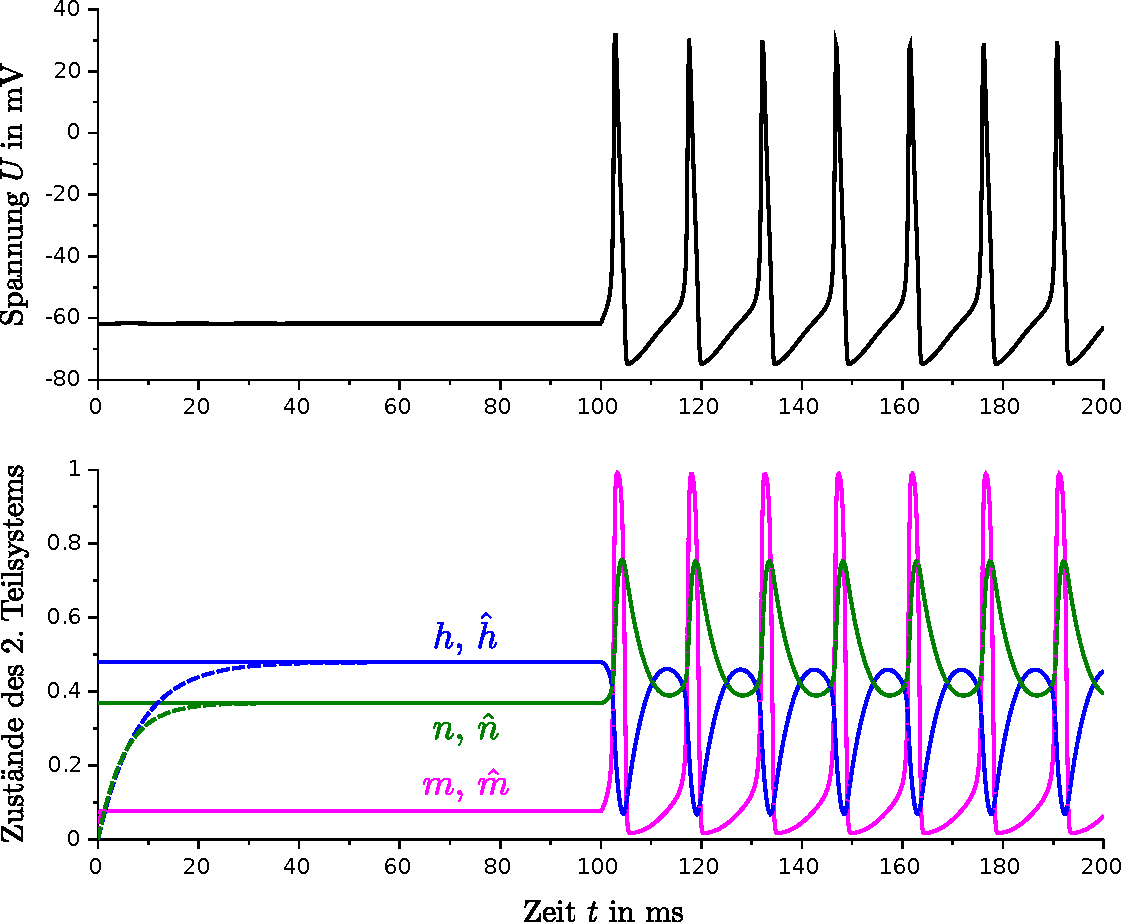
\includegraphics[width=0.95\textwidth]{Hodgkin_Sim}
\par\end{centering}
\caption{Simulierter Spannungsverlauf des Hodgkin-Huxley-Modells (oben), Trajektorien
der internen Dynamik von System und Beobachter (unten)\label{fig:hodgkin-huxley-simulation}}

\end{figure}
\end{example}

\begin{remark}
Der starke Beobachter~(\ref{eq:uio-beobachter}) lässt sich dahingehend
erweitern, dass man simultan auch eine (nicht asymptotische) Schätzung
des Eingangs erhält. Dabei nutzt man Beobachter-Filter-Kombinationen,
die in~\cite{goel2005tech,roebenack2007medjmc,roebenack2009ijss,roebenack2009ndst}
an verschiedenen Zellmodellen erprobt werden.
\end{remark}

\bibliographystyle{babalpha}
\bibliography{dynamic}




\chapter[Beobachterentwurf mittels  Linearisierung der Fehlerdynamik]{Beobachterentwurf mittels exakter bzw. näherungsweiser Linearisierung
der Fehlerdynamik\label{cha:Beobachter-Normalform}}

Normalformen spielen beim Entwurf nichtlinearer Beobachter eine große
Rolle. Kann man ein System in eine Form überführen, bei der die Nichtlinearitäten
ausschließlich von den Messgrößen abhängen, ist der Entwurf eines
Beobachters mit exakt linearer Fehlerdynamik vergleichsweise einfach.
Eine solche Form ist die Beobachternormalform. Die Transformation
in diese Form und damit verbunden die Linearisierung des Beobachtungsfehlers
ist aufgrund restriktiver Existenzbedingungen bzw. einer aufwendigen
Berechnung in der regelungstechnischen Praxis kaum anzutreffen. Bei
genauerer Betrachtung eröffnen sich jedoch etliche Möglichkeiten zur
Berechnung bzw. zur Approximation eines Beobachters mit linearer Fehlerdynamik.
In diesem Kapitel werden Existenzbedingungen und Berechnungsmethoden
vorgestellt.\footnote{Das Kapitel basiert sich an dem Übersichtsbeitrag Röbenack, K.: Entwurf
nichtlinear Beobachter mit linearer und näherungsweise linearer Fehlerdynamik,
Automatisierungstechnik, De Gruyter-Verlag, Berlin, Boston, Jahrgang~58,
Heft~9, S.~489-497, für den der De~Gruyter-Verlag freundlicherweise
eine Nutzungsgenehmigung erteilt hat.}

\section{Linearisierung des Beobachtungsfehlers durch Aufschaltung\label{sec:Linearisierung-durch-Aufschaltung}}

In diesem Abschnitt soll zunächst die grundsätzliche Idee der exakten
Linearisierung des Beobachtungsfehlers durch Aufschaltung illustriert
werden. Angenommen, das zu beobachtende System kann in der Form
\begin{equation}
\dot{x}=Ax+\alpha(y,u),\quad y=c^{T}x\label{eq:lin-beob-fehler-strecke}
\end{equation}
mit dem Zustand~$x$, dem Eingang~$u$, und dem gemessenen Ausgang~$y$
dargestellt werden. Dabei sei der durch das Paar $(A,c^{T})$ beschriebene
lineare Teil beobachtbar. Zusätzlich seien alle auftretenden Nichtlinearitäten
in Abhängigkeit vom Ausgang darstellbar. Diese Nichtlinearitäten werden
in der Eingangs-Ausgangs-Aufschaltung~$\alpha$ zusammengefasst.
Setzt man den Beobachter in der Form
\begin{equation}
\dot{\hat{x}}=A\hat{x}+\alpha(y,u)+l\cdot\left(y-c^{T}\hat{x}\right)\label{eq:lin-beob-fehler-beobachter}
\end{equation}
mit einer Beobachterverstärkung $l\in\R^{n}$ an. so genügt der Beobachtungsfehler
$\tilde{x}=x-\hat{x}$ der linearen zeitinvarianten Differentialgleichung
\begin{equation}
\begin{array}{lcl}
\dot{\tilde{x}} & = & \dot{x}-\dot{\hat{x}}\\
 & = & Ax+\alpha(y,u)-A\hat{x}-\alpha(y,u)-l\cdot\left(y-c^{T}\hat{x}\right)\\
 & = & \left(A-lc^{T}\right)\tilde{x}.
\end{array}\label{eq:lin-beob-fehler-dynamik}
\end{equation}
Über die Verstärkung~$l$ kann man für die Systemmatrix $A-lc^{T}$
der Fehlerdynamik~(\ref{eq:lin-beob-fehler-dynamik}) ein beliebiges
charakteristisches Polynom

\begin{equation}
\det(sI-A+lc^{T})=a_{0}+a_{1}s+\cdots+a_{n-1}s^{n-1}+s^{n}\label{eq:cp}
\end{equation}
vorgeben. Diese Herangehensweise soll an zwei Beispielen vorgestellt
werden:

\begin{example}
\label{exa:inverses-pendel-motor-nf-beobachter}Wir betrachten das
Modell des inversen Pendels mit Gleich\-strom\-antrieb aus Beispiel~\ref{exa:inverses-pendel-gleichstrommotor}:

\begin{equation}
\begin{array}{lcl}
\dot{x}_{1} & = & x_{2}\\
\dot{x}_{2} & = & \frac{mg\ell}{J}\sin x_{1}-\frac{d}{J}x_{2}+\frac{K}{J}x_{3}\\
\dot{x}_{3} & = & -\frac{K}{L}x_{2}-\frac{R}{L}x_{3}+\frac{1}{L}u\\
y & = & x_{1}.
\end{array}\label{eq:inverses-pendel-motor-nf-strecke}
\end{equation}
Als Messgröße steht der Winkel~$x_{1}$, der beispielsweise mit einem
Inkrementgeber erfasst werden kann, zur Verfügung. Die einzige im
System auftretende Nichtlinearität hängt ausschließlich vom Ausgang~$x_{1}$
ab. Der Beobachter setzt sich dann aus einer Kopie des Systems, wobei
die Nichtlinearität vom gemessenen Ausgang gespeist wird, und einem
linearen Korrekturterm zusammen: 
\begin{equation}
\left(\begin{array}{l}
\dot{\hat{x}}_{1}\\
\dot{\hat{x}}_{2}\\
\dot{\hat{x}}_{3}
\end{array}\right)=\left(\begin{array}{c}
\hat{x}_{2}\\
\frac{mg\ell}{J}\sin y-\frac{d}{J}\hat{x}_{2}+\frac{K}{J}\hat{x}_{3}\\
-\frac{K}{L}\hat{x}_{2}-\frac{R}{L}\hat{x}_{3}+\frac{1}{L}u
\end{array}\right)+\left(\begin{array}{l}
l_{1}\\
l_{2}\\
l_{3}
\end{array}\right)\cdot\left(y-\hat{x}_{1}\right)\label{eq:inverses-pendel-motor-nf-beobachter}
\end{equation}
Der Vergleich von~(\ref{eq:inverses-pendel-motor-nf-strecke}) und~(\ref{eq:inverses-pendel-motor-nf-beobachter})
führt auf eine lineare Fehlerdynamik~(\ref{eq:lin-beob-fehler-dynamik}).
Für ein vorgegebenes charakteristisches Polynom~(\ref{eq:cp}) mit
den Koeffizienten $a_{0},a_{1},a_{2}>0$ berechnet man durch Koeffizientenvergleich
oder mit Hilfe der Ackermann-Formel~\cite{acker77,ackermann77} die
Beobachterverstärkung 
\begin{equation}
\begin{array}{lcl}
l_{1} & = & -\frac{R}{L}-\frac{d}{J}+a_{2},\\
l_{2} & = & \frac{-JK^{2}L+\left(a_{1}J^{2}-a_{2}dJ+d^{2}\right)L^{2}-J\left(a_{2}J-d\right)LR+J^{2}R^{2}}{J^{2}L^{2}},\\
l_{3} & = & -\frac{\left(a_{2}J-d\right)K^{2}L^{2}-a_{0}J^{2}L^{3}+JL\left(a_{1}JL-2K^{2}\right)R-a_{2}J^{2}LR^{2}+J^{2}R^{3}}{JKL^{3}}.
\end{array}\label{eq:inverses-pendel-motor-nf-verstaerkung}
\end{equation}
\end{example}

\begin{example}
\label{exa:inverses-pendel-elastisch}Wir betrachten wiederum einen
Manipulator in der Form eines inversen Pendels (siehe Abb.~\ref{fig:Inverses-Pendel-elastisch}).
Der Antrieb erfolgt über ein eingeprägtes Drehmoment~$u$, welches
den Winkel~$q_{1}$ beeinflusst. Der Antrieb ist über eine elastische
Welle, die als Torsionsfeder mit der Federkonstanten~$k$ modelliert
wird, mit dem Manipulatorarm verbunden. Die Position des Manipulatorarms
wird durch den Relativwinkel~$q_{2}$ beschrieben. Der Manipulator
habe beim Antrieb das Trägheitsmoment~$J_{1}$ und hinsichtlich des
Manipulatorarms das Trägheitsmoment~$J_{2}$. Am Ende des Manipulatorarms
der Länge~$\ell$ befinde sich eine Last mit der Masse~$m$.

Das System hat die kinetische Energie
\[
T=\frac{J_{1}}{2}\dot{q}_{1}^{2}+\frac{J_{2}}{2}\left(\dot{q}_{1}+\dot{q}_{2}\right)^{2}
\]
und die potentielle Energie
\[
V=m\ell\left(\cos(q_{1}+q_{2})-1\right)+\frac{k}{2}q_{2}^{2}.
\]
Aus der zugehörigen Bewegungsgleichung erhält man mit $x=(q_{1},\dot{q}_{1},q_{2},\dot{q}_{2})^{T}$
das Zustandsraummodell
\begin{equation}
\left(\begin{array}{l}
\dot{x}_{1}\\
\dot{x}_{2}\\
\dot{x}_{3}\\
\dot{x}_{4}
\end{array}\right)=\left(\begin{array}{c}
x_{2}\\
\frac{k}{J_{1}}x_{3}+\frac{1}{J_{1}}u\\
x_{4}\\
\frac{mg\ell}{J_{2}}\sin(x_{1}+x_{3})-\left(\frac{1}{J_{1}}+\frac{1}{J_{2}}\right)kx_{3}-\frac{u}{J_{1}}
\end{array}\right).\label{eq:inverses-pendel-elastisch}
\end{equation}
Werden die Winkel~$x_{1}$ und~$x_{3}$ oder deren Summe $x_{1}+x_{3}$
gemessen, dann kann die in~(\ref{eq:inverses-pendel-elastisch})
auftretende Nichtlinearität $\sin(x_{1}+x_{3})$ beim Beobachterentwurf
vollständig kompensiert werden~\cite{nicosia88}.
\end{example}
\begin{figure}
\begin{centering}
\resizebox{0.4\textwidth}{!}{\input{inv_pendel_elastisch.pdftex_t}}
\par\end{centering}
\caption{Inverses Pendel, welches elatisch mit dem Antrieb gekoppelt ist\label{fig:Inverses-Pendel-elastisch}}
\end{figure}


\section{Normalfrom-Beobachter\label{sec:Normal-Form-Observer}}

\subsection{Beobachter-Struktur}

Die in Abschnitt~\ref{sec:Linearisierung-durch-Aufschaltung} beschriebene
Herangehensweise wird nachfolgend systematisiert. In der Regel wird
das zu untersuchende System nicht unmittelbar in der Form~(\ref{eq:lin-beob-fehler-strecke})
vorliegen. In etlichen Fällen ist aber eine derartige Darstellung
in anderen Koordinaten möglich. Dazu wird in diesem Abschnitt die
Beobachternormalform eingeführt.

Man betrachte ein nichtlineares System 
\begin{equation}
\dot{x}=F(x,u),\quad y=h(x).\label{eq:plant}
\end{equation}
Die Menge $\mathcal{M}\subseteq\R^{n}$ sei offen und die Menge $\mathcal{U}\subseteq\R^{m}$
beliebig. Die Abbildungen $F:\mathcal{M}\times\mathcal{U}\to\R^{n}$
und $h:\mathcal{M}\to\R$ seien ausreichend glatt. Damit ist~$F$
ein vom Eingang abhängiges Vektorfeld und~$h$ ein Skalarfeld. Angenommen,
in der Umgebung eines Punktes $p\in\mathcal{M}$ gibt es einen Diffeomorphismus
\begin{equation}
z=T(x)\quad\textrm{mit}\quad x=S(z),\label{eq:TS}
\end{equation}
der das System~(\ref{eq:plant}) in die Form 
\begin{equation}
\dot{z}=Az+\alpha(c^{T}z,u),\quad y=\gamma(c^{T}z)\label{eq:nf}
\end{equation}
überführt, wobei das Paar $(A,c^{T})$ in der \emph{dualen} \emph{Brunovský-Normalform}\index{Brunovský-Normalform!duale}\index{Normalform!duale Brunovský-}~\cite{brunovsky70}
vorliege: 
\begin{equation}
A=\left(\begin{array}{cccc}
0 & 0 & \cdots & 0\\
1 & 0 & \ddots & \vdots\\
 & \ddots & \ddots & 0\\
0 &  & 1 & 0
\end{array}\right),\quad c^{T}=\left(\begin{array}{cccc}
0 & \cdots & 0 & 1\end{array}\right).\label{eq:AC}
\end{equation}
Die Form~(\ref{eq:nf}) entspricht der \emph{Beobachter\-normal\-form}
(engl. \emph{observer canonical form})~\cite{zeitz85,zeitz89}\index{Beobachternormalform}\index{Normalform!Beobachter-}
mit der zusätzlichen Ausgangstransformation~$\gamma$ (siehe Abb.~\ref{fig:Beobachter-Normalform}).
Die Abbildung~$\gamma$ muss dabei invertierbar sein. Die vektorwertige
Abbildung~$\alpha$ berücksichtigt die im System auftretenden Nichtlinearitäten.
Dabei fungiert $\alpha(\gamma^{-1}(y),u)$ als Eingangs-Ausgangs-Aufschaltung. 

\begin{figure}
\begin{centering}
\resizebox{0.7\textwidth}{!}{\input{bild-nf2.pdftex_t}}
\par\end{centering}
\caption{Beobachternormalform~(\ref{eq:nf}), Quelle:~\cite{roebenack2010at}\label{fig:Beobachter-Normalform}}
\end{figure}

Für ein System der Form~(\ref{eq:nf}) ist der Beobachterentwurf
sehr einfach. Ein Beobachter der Form 
\begin{equation}
\begin{array}{ccl}
\dot{\hat{z}} & = & A\hat{z}+\alpha(\gamma^{-1}(y),u)+l(\gamma^{-1}(y)-c^{T}\hat{z})\\
\hat{x} & = & S(\hat{z})
\end{array}\label{eq:obs-in-nf}
\end{equation}
mit dem Vektor $l\in\R^{n}$ (siehe Abb.~\ref{fig:Normalform-Beobachter})
führt auf einen Beobachtungsfehler $\tilde{z}=z-\hat{z}$, welcher
dem linearen zeit\-invarianten Differential\-gleichungs\-system
\begin{equation}
\dot{\tilde{z}}=(A-lc^{T})\tilde{z}\label{eq:error-dgl-nf}
\end{equation}
genügt. Da das Paar $(A,c^{T})$ beobachtbar ist, lassen sich die
Eigenwerte von $A-lc^{T}$ beliebig zuweisen. Für ein gewünschtes
charakteristisches Polynom~(\ref{eq:cp}) der Fehlerdynamik~(\ref{eq:error-dgl-nf})
ist der Vektor~$l$ entsprechend $l=(a_{0},\ldots,a_{n-1})^{T}$
zu wählen. Legt man~$l$ derart fest, dass alle Wurzeln von~(\ref{eq:cp})
in der offenen linken Halbebene liegen, dann ist die Ruhelage $\tilde{z}=0$
von~(\ref{eq:error-dgl-nf}) exponentiell (und damit auch asymptotisch)
stabil. 

\begin{figure}
\begin{centering}
\resizebox{0.85\textwidth}{!}{\input{bild-nfbeob1.pdftex_t}}
\par\end{centering}
\caption{Normalform-Beobachter~(\ref{eq:obs-in-nf})\label{fig:Normalform-Beobachter}}
\end{figure}

Der Beobachter~(\ref{eq:obs-in-nf}) basiert unmittelbar auf der
Normalform~(\ref{eq:nf}). Daher nennt man ihn \emph{Normalform-Beobachter}\index{Beobachter!Normalform-}.\index{Normalform-Beobachter}
Mitunter ist es wünschenswert, den Beobachter~(\ref{eq:obs-in-nf})
direkt in den Originalkoordinaten zu implementieren:
\begin{equation}
\dot{\hat{x}}=F(\hat{x},u)+k_{\infty}(\hat{x},y,u).\label{eq:ons-orig}
\end{equation}
Der Korrekturterm hat dann die Form 
\begin{equation}
\begin{array}{ccl}
k_{\infty}(\hat{x},y,u) & = & \left(T^{\prime}(\hat{x})\right)^{-1}\left[\alpha(\gamma^{-1}(y),u)-\alpha(\gamma^{-1}(h(\hat{x})),u)\right.\\
 &  & \left.+\,l(\gamma^{-1}(y)-\gamma^{-1}(h(\hat{x})))\right].
\end{array}\label{eq:correction-term-nf-obs}
\end{equation}

\begin{remark}
Mit dem beschriebenen Zugang ergibt sich eine Fehlerdynamik, die in
den transformierten Koordinaten einer linearen zeit\-invarianten
Differentialgleichung~(\ref{eq:error-dgl-nf}) genügt. Daher spricht
man auch von einer \emph{exakten Linearisierung des Beobachtungsfehlers}.
Dieses Konzept ist auch bei Systemen mit mehreren Ausgängen anwendbar~\cite{krener85observer,xia88,xia89}
und kann mit einer Parameter\-adaption kombiniert werden~\cite{marino1990,marino1992,marino1995,marino1995book}.
Die Linearisierung des Beobachtungsfehlers entspricht in gewisser
Weise der vollständigen Linearisierung (Eingangs-Zustands-Linearisierung)
beim Reglerentwurf. Ähnlich wie bei der Regelung ist auch beim Beobachterentwurf
mitunter nur eine \emph{partielle Linearisierung des Beobachtungsfehlers}
möglich. Entsprechende Entwurfsverfahren werden beispielsweise in~\cite{jo2000b,jo2002,roebenack2005syncod,roebenack2006amcs,roebenack2007iet,roebenack2007ndst}
beschrieben.
\end{remark}

\begin{remark}
Mitunter wird für das System~(\ref{eq:nf}) mit dem Beobachter~(\ref{eq:obs-in-nf})
eine andere Darstellungsform favorisiert. Seien 
\[
\check{A}:=A-lc^{T}\quad\mbox{und}\quad\check{\alpha}(z_{n},u):=\alpha(z_{n},u)+lz_{n},
\]
wobei der Vektor $l\in\R^{n}$ so zu wählen ist, dass die Matrix~$\check{A}$
nur Eigenwerte in der linken offenen Halbebene besitzt. Das System~(\ref{eq:nf})
lässt sich dann in der Form 
\[
\begin{array}{ccl}
\dot{z} & = & Az+\alpha(z_{n},u)\\
 & = & Az-lc^{T}z+lc^{T}z+\alpha(z_{n},u)\\
 & = & \check{A}z+\check{\alpha}(\gamma^{-1}(y),u)
\end{array}
\]
angeben. Der Beobachter~(\ref{eq:obs-in-nf}) vereinfacht sich zu
\[
\begin{array}{ccl}
\dot{\hat{z}} & = & A\hat{z}+\alpha(z_{n},u)+l(z_{n}-c^{T}\hat{z})\\
 & = & (A-lc^{T})\hat{z}+\alpha(z_{n},u)+lz_{n}\\
 & = & \check{A}\hat{z}+\check{\alpha}(\gamma^{-1}(y),u)
\end{array}
\]
mit $\hat{x}=S(\hat{z})$. Als Fehlerdifferentialgleichung erhält
man wiederum Gl.~(\ref{eq:error-dgl-nf}), d.\,h. $\dot{\tilde{z}}=\check{A}\tilde{z}$.
Diese Form von Strecke und Beobachter ist bei verschiedenen neueren
Zugängen zur exakten bzw. approximativen Linearisierung des Beobachtungsfehlers
zu finden (siehe~\cite{kazantzis1998,krener2002,xiao2006,deutscher2006,deutscher2007}
sowie Anmerkung~\ref{rem:Boebachter-mit-Hilfssatz-von-Ljapunov}).
\end{remark}

\begin{remark}
\label{rem:endliche-Einstellzeit}Bei der Fehlerdifferentialgleichung~(\ref{eq:error-dgl-nf})
des Normalformbeobachters~ (\ref{eq:obs-in-nf}) kann man durch geeignete
Wahl des Vektors $l\in\R^{n}$ die Eigenwerte der Systemmatrix $A-lc^{T}$
in der komplexen Ebene beliebig weit links anordnen und damit die
Konvergenzgeschwindigkeit vorgeben. Bei einem Anfangswert $\tilde{z}(0)\neq0$
wird die Ruhelage $\tilde{z}=0$ von~(\ref{eq:error-dgl-nf}) jedoch
erst in unendlicher Zeit erreicht. Für lineare Systeme kann man durch
geeignete Nutzung eines Totzeitgliedes eine endliche Einstellzeit
vorgeben~\cite{engel2002}. Dieser Zugang lässt sich auch für nichtlineare
Systeme, die in die Beobachternormalform~(\ref{eq:nf}) transformierbar
sind, erweitern~\cite{menold2003cdc}.
\end{remark}

\subsection{Reduzierter Normalform-Beobachter}

Bei der Normalform~(\ref{eq:nf}) lässt sich die letzte Komponente
des Zustands mit $z_{n}=\gamma^{-1}(y)$ direkt aus dem Ausgang rekonstruieren
und muss daher nicht geschätzt werden. Folglich ist es naheliegend,
zur Rekonstruktion der verbleibenden $n-1$ Zustandsgrößen $z_{1},\ldots,z_{n-1}$
einen \emph{reduzierten} Beobachter\index{Beobachter!reduzierter}
einzusetzen. 

Die Herleitung eines reduzierten Zustandsbeobachters ist in Analogie
zum linearen Fall möglich~\cite[Abschnitt~{7.4.2}]{ludyk1995-2}.
Durch Streichen der letzten Differentialgleichung in der Normalform~(\ref{eq:nf})
erhält man das System 
\begin{equation}
\dot{\bar{z}}=\bar{A}\bar{z}+\bar{\alpha}(\bar{c}^{T}z,u)\label{eq:reduzierte-nf}
\end{equation}
mit 
\[
\bar{z}=\left(\begin{array}{c}
z_{1}\\
\vdots\\
z_{n-1}
\end{array}\right)\quad\mbox{und}\quad\bar{\alpha}(z_{n},u)=\left(\begin{array}{c}
\alpha_{1}(z_{n},u)\\
\vdots\\
\alpha_{n-1}(z_{n},u)
\end{array}\right).
\]
Das Paar $(\bar{A},\bar{c}^{T})$ mit $\bar{A}\in\R^{(n-1)\times(n-1)}$
und $\bar{c}\in\R^{n-1}$ liegt in der dualen Brunovský-Normalform
der Ordnung $n-1$ vor (siehe Gl.~(\ref{eq:AC})). Der Beobachtungsfehler
$\tilde{\bar{z}}=\bar{z}-\hat{\bar{z}}$ soll einer linearen zeit\-invarianten
Differentialgleichung 
\begin{equation}
\dot{\tilde{\bar{z}}}=\left(\bar{A}-\bar{l}\,\bar{c}^{T}\right)\tilde{\bar{z}}\label{eq:reduziert-error-dgl}
\end{equation}
genügen, wobei der Vektor $\bar{l}=(p_{0},\ldots,p_{n-2})^{T}\in\R^{n-1}$
die Koeffizienten eines vorgegebenen charakteristischen Polynoms vom
Grad $n-1$ enthält. Der Vergleich von~(\ref{eq:reduzierte-nf})
und~(\ref{eq:reduziert-error-dgl}) liefert für den Zustand $\hat{\bar{z}}=\bar{z}-\tilde{\bar{z}}$
die Differentialgleichung
\begin{equation}
\dot{\hat{\bar{z}}}=\bar{A}\hat{\bar{z}}+\bar{\alpha}(z_{n},u)+\bar{l}\tilde{\bar{z}}_{n-1}\label{eq:red-nf-beob-schritt1}
\end{equation}
mit $\tilde{\bar{z}}_{n-1}=\bar{z}_{n-1}-\hat{\bar{z}}_{n-1}$. In
dieser Gleichung wird $\bar{z}_{n-1}=z_{n-1}$ benötigt. Diese Größe
lässt sich aus der letzten Differentialgleichung 
\[
\dot{z}_{n}=z_{n-1}+\alpha_{n}(z_{n},u),\quad z_{n}=\gamma^{-1}(y)
\]
der Normalform~(\ref{eq:nf}) rekonstruieren: 
\[
\bar{z}_{n-1}=z_{n-1}=\frac{\d}{\d t}\left(\gamma^{-1}(y)\right)-\alpha_{n}(\gamma^{-1}(y),u).
\]
Durch Einsetzen in~(\ref{eq:red-nf-beob-schritt1}) erhält man 
\[
\begin{array}{ccl}
\dot{\hat{\bar{z}}} & = & \bar{A}\hat{\bar{z}}+\bar{\alpha}(\gamma^{-1}(y),u)+\bar{l}\left(\frac{\d}{\d t}\left(\gamma^{-1}(y)\right)-\alpha_{n}(\gamma^{-1}(y),u)-\bar{c}^{T}\hat{\bar{z}}\right)\\
 & = & \left(\bar{A}-\bar{l}\,\bar{c}^{T}\right)\hat{\bar{z}}+\bar{\alpha}(\gamma^{-1}(y),u)+\bar{l}\left(\frac{1}{\gamma^{\prime}(y)}\dot{y}-\alpha_{n}(\gamma^{-1}(y),u)\right).
\end{array}
\]
Diese Gleichung kann wegen der auf der rechten Seite auftretenden
Zeit\-ab\-leitung~$\dot{y}$ noch nicht für die Zustandsbeobachtung
eingesetzt werden. Zur Elimination von~$\dot{y}$ wird für den Beobachter
die Koordinatentransformation 
\[
\begin{array}{ccccc}
w & = & \hat{\bar{z}} & - & \bar{l}\gamma^{-1}(y)\\
\hat{\bar{z}} & = & w & + & \bar{l}\gamma^{-1}(y)
\end{array}
\]
eingeführt. Dann gilt 
\[
\begin{array}{ccl}
\dot{w} & = & \frac{\d}{\d t}\left(\hat{\bar{z}}-\bar{l}\gamma^{-1}(y)\right)\\
 & = & \dot{\hat{\bar{z}}}-\bar{l}\frac{\d}{\d t}\left(\gamma^{-1}(y)\right)\\
 & = & \left(\bar{A}-\bar{l}\,\bar{c}^{T}\right)\hat{\bar{z}}+\bar{\alpha}(\gamma^{-1}(y),u)+\bar{l}\left(\frac{\d}{\d t}\left(\gamma^{-1}(y)\right)-\alpha_{n}(\gamma^{-1}(y),u)\right)-\bar{l}\frac{\d}{\d t}\left(\gamma^{-1}(y)\right)\\
 & = & \left(\bar{A}-\bar{l}\,\bar{c}^{T}\right)\hat{\bar{z}}+\bar{\alpha}(\gamma^{-1}(y),u)-\bar{l}\alpha_{n}(\gamma^{-1}(y),u)\\
 & = & \left(\bar{A}-\bar{l}\,\bar{c}^{T}\right)\left(w+\bar{l}\gamma^{-1}(y)\right)+\bar{\alpha}(\gamma^{-1}(y),u)-\bar{l}\alpha_{n}(\gamma^{-1}(y),u)\\
 & = & \left(\bar{A}-\bar{l}\,\bar{c}^{T}\right)w+\left(\bar{A}-\bar{l}\,\bar{c}^{T}\right)\bar{l}\gamma^{-1}(y)+\bar{\alpha}(\gamma^{-1}(y),u)-\bar{l}\alpha_{n}(\gamma^{-1}(y),u).
\end{array}
\]
Die letzte Gleichung liefert den \emph{reduzierten Normalform-Beobachter}\index{Normalform-Beobachter!reduzierter}
\begin{equation}
\dot{w}=\left(\bar{A}-\bar{l}\,\bar{c}^{T}\right)w+\underbrace{\left(\bar{A}-\bar{l}\,\bar{c}^{T}\right)\bar{l}\gamma^{-1}(y)+\bar{\alpha}(\gamma^{-1}(y),u)-\bar{l}\alpha_{n}(\gamma^{-1}(y),u)}_{{\displaystyle \kappa(\gamma^{-1}(y),u)}}\label{eq:red-nf-beob}
\end{equation}
mit dem Korrekturterm~$\kappa$, wobei der Originalzustand mittels
\begin{equation}
\hat{z}=\left(\begin{array}{c}
w+\bar{l}\gamma^{-1}(y)\\
\gamma^{-1}(y)
\end{array}\right),\quad\hat{x}=S(\hat{z})\label{eq:red-nf-ruecktransf}
\end{equation}
rekonstruiert wird. Das zugehörige Strukturbild ist in Abb.~\ref{fig:Reduzierter-Normalformbeobachter}
dargestellt.

\begin{figure}
\begin{centering}
\resizebox{0.85\textwidth}{!}{\input{bild-reduzierter-nf-beob1.pdftex_t}}
\par\end{centering}
\caption{Reduzierter Normalformbeobachter~(\ref{eq:red-nf-beob}) mit Rücktransformation~(\ref{eq:red-nf-ruecktransf})\label{fig:Reduzierter-Normalformbeobachter}}
\end{figure}


\section{Existenz und Berechnung der Beobachternormalform}

\subsection{Existenz und Berechnung der Normalform nach Byrnes und Isidori\label{subsec:Berechnung-nach-Byrnes-Isidori}}

Die Schwierigkeit beim Entwurf eines Normalform-Beobachters besteht
in der Existenz der Normalform~(\ref{eq:nf}) sowie in der konkreten
Berechnung der Transformation~(\ref{eq:TS}). Für die folgenden Betrachtungen
ist es zweckmäßig, das zu beobachtende System~(\ref{eq:plant}) in
der Form 
\begin{equation}
\dot{x}=f(x)+g(x,u),\quad y=h(x),\label{eq:plant-fg}
\end{equation}
mit den Abbildungen $f:\mathcal{M}\to\R^{n}$ und $g:\mathcal{M}\times\mathcal{U}\to\R^{n}$
anzugeben. Diese Abbildungen seien durch 
\[
f(x)=F(x,0)\quad\mbox{und}\quad g(x,u)=F(x,u)-F(x,0)
\]
festgelegt. Die Beobachtbarkeitsmatrix\index{Beobachtbarkeitsmatrix}~$Q_{B}$
ist die Jacobimatrix der Beobachtbarkeitsabbildung\index{Beobachtbarkeitsabbildung}~$q:\mathcal{M}\to\R^{n}$,
d.\,h. 
\begin{equation}
q(x)=\left(\begin{array}{c}
h(x)\\
L_{f}h(x)\\
\vdots\\
L_{f}^{n-1}h(x)
\end{array}\right),\quad Q_{B}(x)=q^{\prime}(x)=\left(\begin{array}{c}
dh(x)\\
L_{f}dh(x)\\
\vdots\\
L_{f}^{n-1}dh(x)
\end{array}\right),\label{eq:Q}
\end{equation}
vgl. Abschnitt~\ref{subsec:Beobachtbarkeit-autonom}. Der sogenannte
\emph{Start\-vektor} bzw. das sog. \emph{Start\-vektor\-feld}\index{Startvektorfeld}\footnote{Mit dem Vektorfeld~$v$ wird zyklisch der gesamte Raum für das transformierte
System aufgespannt.} ist die Lösung des Gleichungssystems
\begin{equation}
Q_{B}(x)\,v(x)=\beta(h(x))\,\frac{\partial}{\partial x_{n}}\label{eq:v}
\end{equation}
mit einer skalarwertigen Funktion~$\beta$. Der folgende Satz gibt
die Existenzbedingungen für die Normalform~(\ref{eq:nf}) an~\cite{krener83,marino1990}:
\begin{theorem}
\label{thm:existence}In einer Umgebung von $p\in\mathcal{M}$ existiert
genau dann ein lokaler Diffeomorphismus~(\ref{eq:TS}), der das System~(\ref{eq:plant-fg})
in die Normalform~(\ref{eq:nf}) mit einem lokalen Diffeomorphismus~$\gamma$
überführt, wenn für eine geeignete Funktion~$\beta$ mit $\beta(h(p))\neq0$
die Bedingungen
\begin{enumerate}
\item \label{enu:ki1}$\rank\,Q_{B}(p)=n$

\item \label{enu:ki2}$[\ad_{-f}^{i}v,\ad_{-f}^{j}v](x)=0$ für $0\leq i,j\leq n-1$
\item \label{enu:ki3}$[g,\ad_{-f}^{i}v](x,u)=0$ für $0\leq i\leq n-2$
\end{enumerate}
für alle $x$ in einer Umgebung von~$p$ und für alle $u\in\mathcal{U}$
erfüllt sind. Es gibt einen globalen Diffeomrophismus~(\ref{eq:TS}),
wenn die Bedingungen~\ref{enu:ki1}-\ref{enu:ki3} in $\mathcal{M}=\R^{n}$
gelten und zusätzlich
\begin{enumerate}[start=4]
\item \label{enu:ki4}$\ad_{-f}^{i}v$ für $0\leq i<n$ vollständige Vektorfelder\index{Vektorfeld!vollständiges}
sind.
\end{enumerate}
\end{theorem}
Der folgende Beweis widmet sich der Existenz einer lokalen Koordinatentransformation. 
\begin{svmultproof2}
\hinreichend\ Die Bedingungen \ref{enu:ki1}-\ref{enu:ki3} seien
in einer Umgebung von $p\in\mathcal{M}$ erfüllt. Wegen Bedingung~\ref{enu:ki1}
ist das lineare Gls.~(\ref{eq:v}) (eindeutig) lösbar bezüglich~$v$.
Zeilenweise kann man Gls.~(\ref{eq:v}) auch in der Form 
\begin{equation}
L_{v}L_{f}^{i}h(x)=\left\langle \d L_{f}^{i}h(x),v(x)\right\rangle =\left\{ \begin{array}{ccl}
0 & \mbox{für} & i=0,\ldots,n-2,\\
\beta(h(x)) & \mbox{für} & i=n-1.
\end{array}\right.\label{eq:proof-obsnf-gl0}
\end{equation}
schreiben. Wegen 
\begin{equation}
\begin{array}{l}
\left(\begin{array}{c}
\d h(p)\\
\vdots\\
\d L_{f}^{n-1}h(p)
\end{array}\right)\left(v(p),\,\ad_{-f}v(p),\,\cdots,\,\ad_{-f}^{n-1}v(p)\right)=\\
=\left(\begin{array}{cccc}
0 & \cdots & 0 & \beta(h(p))\\
\vdots & \qdots & \qdots & *\\
0 & \qdots & \qdots & \vdots\\
\beta(h(p)) & * & \cdots & *
\end{array}\right)
\end{array}\label{eq:proof-obsnf-gl1}
\end{equation}
sind die Vektorfelder $v,\ad_{-f}v,\ldots,\ad_{-f}^{n-1}v$ in einer
Umgebung von~$p$ linear unabhängig (vgl. Lemma~\ref{lem:Lin-Unabh-Kovektoren}).
In Verbindung mit Bedingung~\ref{enu:ki2} garantiert der Begradigungssatz
(Satz~\ref{thm:simultane-begradigung-von-VF}) die Existenz eines
lokalen Diffeomorphismus~(\ref{eq:TS}) mit 
\begin{equation}
T_{*}\ad_{-f}^{i}v=\frac{\partial}{\partial z_{i+1}}\quad\mbox{für}\quad i=0,\ldots,n-1.\label{eq:proof-obsnf-gl2}
\end{equation}
 Der Diffeomorphismus~(\ref{eq:TS}) transformiert die im System~(\ref{eq:plant-fg})
auftretenden Abbildungen in die Form 
\begin{equation}
\begin{array}{lcl}
\bar{f}(z) & = & T_{*}f(S(z)),\\
\bar{g}(z,u) & = & T_{*}g(S(z),u),\\
\bar{h}(z) & = & h(S(z)).
\end{array}\label{eq:proof-obsnf-bar-groessen}
\end{equation}
Wegen Gls.~(\ref{eq:proof-obsnf-gl1}) gilt
\begin{equation}
\frac{\partial}{\partial z_{i+1}}\bar{h}=\left\langle \d h,\ad_{-f}^{i}v\right\rangle =\left\{ \begin{array}{ccl}
0 & \mbox{für} & i=0,\ldots,n-2,\\
\beta(h(x)) & \mbox{für} & i=n-1,
\end{array}\right.\label{eq:proof-obsnf-dh-beta}
\end{equation}
d.\,h. der Gradient von~$\bar{h}$ hat die Form 
\[
\bar{h}^{\prime}(z)=\left(\begin{array}{cccc}
0 & \cdots & 0 & *\end{array}\right).
\]
Folglich hat die Ausgangsabbildung~$\bar{h}$ die in Gl.~(\ref{eq:nf})
angegebene Form d.\,h. es besteht nur eine Abhängigkeit von der letzten
Zustandskomponente~$z_{n}$.

Als nächstes wird das Vektorfeld 
\[
\bar{f}=\bar{f}_{1}\frac{\partial}{\partial z_{1}}+\cdots+\bar{f}_{n}\frac{\partial}{\partial z_{n}}
\]
betrachtet. Mit~(\ref{eq:proof-obsnf-gl2}) gilt 
\[
\begin{array}{ccl}
\tfrac{\partial}{\partial z_{i+1}} & = & T_{*}\ad_{-f}^{i}v\\
 & = & T_{*}[-f,\ad_{-f}^{i-1}v]\\
 & = & [-T_{*}f,T_{*}\ad_{-f}^{i-1}v]\\
 & = & [-\bar{f},\tfrac{\partial}{\partial z_{i}}]\\
 & = & \sum_{j=1}^{n}\left(\left(\tfrac{\partial}{\partial z_{i}}\bar{f}_{j}\right)\tfrac{\partial}{\partial z_{j}}\right)
\end{array}
\]
für $i=1,\ldots,n-1$. Ein Vergleich beider Seiten der Gleichung liefert
\[
\frac{\partial\bar{f}_{j}}{\partial z_{i}}=\left\{ \begin{array}{ccccc}
0 & \mbox{für} & j & \neq & i+1\\
1 & \mbox{für} & j & = & i+1
\end{array}\right.
\]
mit $1\leq i\leq n-1$ und $1\leq j\leq n$. Die $n\times n$-Jacobimatrix
von~$\bar{f}$ hat folglich die Form 
\begin{equation}
\bar{f}^{\prime}(z)=\left(\begin{array}{ccccc|c}
0 & 0 & \cdots & 0 & 0 & *\\
1 & 0 &  & \vdots & 0 & *\\
0 & 1 & \ddots & \vdots & \vdots & \vdots\\
\vdots & 0 & \ddots & 0 & \vdots & \vdots\\
0 & \vdots & \ddots & 1 & 0 & *\\
0 & 0 & \cdots & 0 & 1 & *
\end{array}\right).\label{eq:proof-obsnf-Form-DF}
\end{equation}

Bei dem vom Eingang abhängigen Vektorfeld~$\bar{g}$ geht man ähnlich
vor. Wegen Bedingung~\ref{enu:ki3} und Gl.~(\ref{eq:proof-obsnf-gl2})
gilt 
\[
\begin{array}{ccl}
0 & = & T_{*}[g,\ad_{-f}^{i}v]\\
 & = & [T_{*}g,T_{*}\ad_{-f}^{i}v]\\
 & = & [\bar{g},\frac{\partial}{\partial z_{i+1}}]\\
 & = & -\sum_{j=1}^{n}\left(\left(\tfrac{\partial}{\partial z_{i+1}}\bar{g}_{j}\right)\tfrac{\partial}{\partial z_{j}}\right)
\end{array}
\]
für $i=0,\ldots,n-2$, d.\,h. 
\[
\frac{\partial}{\partial z_{i+1}}\bar{g}_{j}=0\quad\mbox{für}\quad1\leq j\leq n\quad\mbox{und}\quad0\leq i\leq n-2.
\]
Die Jacobimatrix von~$\bar{g}$ hat somit die Form 
\begin{equation}
\frac{\partial\bar{g}}{\partial z}(z,u)=\left(\begin{array}{ccc|c}
0 & \cdots & 0 & *\\
\vdots & \ddots & \vdots & \vdots\\
0 & \cdots & 0 & *
\end{array}\right).\label{eq:proof-obsnf-Form-DG}
\end{equation}
Aus Gln.~(\ref{eq:proof-obsnf-Form-DF}) und~(\ref{eq:proof-obsnf-Form-DG})
folgt, dass das kombinierte Vektorfeld $(\bar{f}+\bar{g})$ die in
Gl.~(\ref{eq:nf}) angegebene Gestalt besitzt.

\notwendig\ Angenommen, es gäbe lokale Diffeomorphismen~(\ref{eq:TS})
und~$\gamma$, die das System~(\ref{eq:plant}) in einer Umgebung
des Punktes~$p$ in die Normalform~(\ref{eq:nf}) überführen. Simultan
wird für das transformierte System~(\ref{eq:nf}) auch die Form~(\ref{eq:proof-obsnf-bar-groessen})
verwendet. Ohne Einschränkung sei $T(p)=0$ (andernfalls Verschiebung
des Koordinatensystems). Die Beobachtbarkeitsmatrix der Normalform
lässt sich leicht berechnen. Zu der Beobachtbarkeitsmatrix~(\ref{eq:Q})
in den Originalkoordinaten besteht folgender Zusammenhang: 
\begin{equation}
\begin{array}{rcl}
Q_{B}(x) & = & {\displaystyle \frac{\partial}{\partial x}}\left(\begin{array}{c}
h(x)\\
\vdots\\
L_{f}^{n-1}h(x)
\end{array}\right)\\
 & = & {\displaystyle \frac{\partial}{\partial z}}\left(\begin{array}{c}
h(S(z))\\
\vdots\\
L_{f}^{n-1}h(S(z))
\end{array}\right){\displaystyle \frac{\partial z}{\partial x}}\\
 & = & {\displaystyle \frac{\partial}{\partial z}}\left(\begin{array}{c}
\bar{h}(z)\\
\vdots\\
L_{\bar{f}}^{n-1}\bar{h}(z)
\end{array}\right){\displaystyle \frac{\partial z}{\partial x}}\\
 & = & \left.\left(\begin{array}{cccc}
0 & \cdots & 0 & \gamma^{\prime}(z_{n})\\
\vdots & \qdots & \qdots & *\\
0 & \qdots & \qdots & \vdots\\
\gamma^{\prime}(z_{n}) & * & \cdots & *
\end{array}\right)\right|_{z=T(x)}\cdot T^{\prime}(x).
\end{array}\label{eq:proof-obnf-Qx-Qz}
\end{equation}
Die Matrizen auf der rechten Seite sind im Punkt~$p$ regulär, weil~$\gamma$
und~$T$ Diffeomorphismen sind. Damit muss auch die Matrix $Q_{B}(p)$
regulär sein, d.\,h. Bedingung~\ref{enu:ki1} ist erfüllt. 

Als nächstes transformieren wir das Vektorfeld~$v$ mittels Pushforward
in die Normalform-Koordinaten: 
\[
\bar{v}(z)=T_{*}v(S(z)).
\]
In den Originalkoordinaten kann das in Gl.~(\ref{eq:v}) definierte
Startvektorfeld auch als Lösung von Gl.~(\ref{eq:proof-obsnf-gl0})
beschrieben werden. Mit Gl.~(\ref{eq:proof-obnf-Qx-Qz}) erhält man
analog in den transformierten Koordinaten die Darstellung 
\[
L_{\bar{v}}L_{\bar{f}}^{i}\bar{h}(z)=\left\langle \d L_{\bar{f}}^{i}\bar{h}(z),\bar{v}(z)\right\rangle =\left\{ \begin{array}{ccl}
0 & \mbox{für} & i=0,\ldots,n-2,\\
\gamma^{\prime}(z_{n}) & \mbox{für} & i=n-1.
\end{array}\right.
\]
Daraus folgt $\beta(h(p))=\gamma^{\prime}(0)\neq0$, so dass die Ausgangstransformation~$\gamma$
ein lokaler Diffeomorphismus ist. Für die Normalform~(\ref{eq:nf})
lässt sich unmittelbar nachrechnen, dass die Bedingungen 
\[
\begin{array}{rclcl}
[\ad_{-\bar{f}}^{i}\bar{v},\ad_{-\bar{f}}^{j}\bar{v}](z) & = & 0 & \mbox{für} & 0\leq i,j\leq n-1\\{}
[\bar{g},\ad_{-\bar{f}}^{i}\bar{v}](z,u) & = & 0 & \mbox{für} & 0\leq i\leq n-2
\end{array}
\]
in einer Umgebung von $z=0$ und für alle $u\in\mathcal{U}$ erfüllt
sind. Aus Proposition~\ref{pro:Lie-Klammer-und-Push-Forward} folgt,
dass die zugehörigen Bedingungen~\ref{enu:ki2} und~\ref{enu:ki3}
auch in den Originalkoordinaten erfüllt sind.
\end{svmultproof2}

Bedingung~\ref{enu:ki1} aus Satz~\ref{thm:existence} ist die lokale
Beobachtbarkeitsbedingung (siehe Abschnitt~\ref{subsec:Beobachtbarkeit-autonom}
und Anmerkung~\ref{rem:stetige-Beobachter}). Die Integrabilitätsbedingung\index{Integrabilitätsbedingung}~\ref{enu:ki2}
ist bei vielen Systemen nicht erfüllt. Allerdings kann man die Klasse
der in die Normalform~(\ref{eq:nf}) transformierbaren Systeme vergrößern,
indem man z.\,B. Zeitskalierungen berücksichtigt~\cite{guay2002,respondek2004}\@.
Bei autonomen Systemen entfällt die Bedingung~\ref{enu:ki3}. 

Selbst wenn die Bedingungen von Satz~\ref{thm:existence} erfüllt
sind, ist die konkrete Berechnung der Normalform~(\ref{eq:nf}) bzw.
des Beobachters~(\ref{eq:ons-orig}) in der Regel sehr schwierig.
Prinzipiell lässt sich dabei wie folgt vorgehen: Ausgehend von der
Beobachtbarkeitsmatrix~(\ref{eq:Q}) bestimmt man den Startvektor~$v$
entsprechend Gl.~(\ref{eq:v}) und die Lie-Klammern $\ad_{-f}v,\ldots,\ad_{-f}^{n-1}v$
für eine geeignete Abbildung~$\beta$. Die Abbildung~$\beta$ ist
dabei so zu wählen, dass Bedingung~\ref{enu:ki2} des Satzes erfüllt
ist. Anschließend fasst man die vektorwertigen Gln.~(\ref{eq:proof-obsnf-gl2})
spaltenweise zu der matrixwertigen Gleichung 
\begin{equation}
I=T^{\prime}(x)\cdot\Pi(x)\label{eq:pde-T}
\end{equation}
mit
\begin{equation}
\Pi(x)=\left(\begin{array}{cccc}
v(x) & \ad_{-f}v(x) & \cdots & \ad_{-f}^{n-1}v(x)\end{array}\right)\label{eq:PI}
\end{equation}
zusammen~\cite{schaffner99}. Die Matrix~$\Pi$ ist dabei die von
den Vektorfeldern~$f$ und~$v$ erzeugte Steuerbarkeitsmatrix (siehe
Anmerkung~\ref{rem:Steuerbarkeitsmatrix}). Bei Gl.~(\ref{eq:pde-T})
handelt es sich um eine partielle Differentialgleichung, die bezüglich~$T$
zu lösen ist. In \textsc{Maple} steht dazu die Routine \texttt{pdesolve}
aus der Bibliothek \texttt{PDEtools} zur Verfügung~\cite{chep-terrab1995}. 

Alternativ kann man die gesuchte Koordinatentransformation~(\ref{eq:TS})
auch unmittelbar auf Basis des im Beweis von Satz~\ref{thm:existence}
verwendeten Begradigungssatzes berechnen. Dazu bestimmt man die Flüsse
der in Gl.~(\ref{eq:PI}) auftretenden Vektor\-felder und bildet
die nachfolgende Flussverknüpfung\index{Fluss!Verkettung} (siehe
Beweis von Satz~\ref{thm:simultane-begradigung-von-VF}):
\begin{equation}
x=S(z)=\varphi_{z_{1}}^{v}\circ\varphi_{z_{2}}^{\ad_{-f}v}\circ\cdots\circ\varphi_{z_{n}}^{\ad_{-f}^{n-1}v}(p).\label{eq:verknuepfung-der-fluesse}
\end{equation}
Mit zunehmender Ordnung der Lie-Klammern werden die Vektor\-felder
$v,ad_{-f}v,\ldots,ad_{-f}^{n-1}v$ in der Regel komplizierter. Bei
dem potentiell kompliziertesten Vektor\-feld $ad_{-f}^{n-1}v$ benötigt
man jedoch nicht den allgemeinen Fluss, sondern nur die Lösung einer
Anfangswertaufgabe, die sich durch geeignete Wahl des Anfangswertes~$p$
oft vereinfachen lässt. Die Umkehrung von~$S$ liefert die Hintransformation~$T$.

Aus der Kenntnis der Transformation~(\ref{eq:TS}) erhält man die
Normalform~(\ref{eq:nf}) bzw. die Abbildungen~$\alpha$ und~$\gamma$
mit Hilfe von Gl.~(\ref{eq:proof-obsnf-bar-groessen}), d.\,h. 
\[
Az+\alpha(z_{n},u)=T_{*}F(S(z))=\left(S^{\prime}(z)\right)^{-1}F(S(z))\quad\mbox{und}\quad\gamma(z_{n})=h(S(z)).
\]
Zwischen den Funktionen~$\beta$ und~$\gamma$ besteht wegen Gl.~(\ref{eq:proof-obsnf-dh-beta})
der Zusammenhang 
\begin{equation}
\gamma^{\prime}(z_{n})=\beta(h(x))=\beta(h(S(z))).\label{eq:dgamma-beta}
\end{equation}
Die Ausgangstransformation~$\gamma$ lässt sich daher bis auf eine
Integrationskonstante durch 
\[
\gamma(z_{n})=\int\beta(h(S(z)))\,\d z_{n}
\]
bestimmen.

\begin{example}
\label{exa:van-der-Pol-Krener-Isidori}Man betrachte den van der Pol-Oszillator
\begin{equation}
\begin{array}{lcl}
\dot{x}_{1} & = & x_{2}\\
\dot{x}_{2} & = & -x_{1}+x_{2}(1-x_{1}^{2})+x_{1}u\\
y & = & x_{1}
\end{array}\label{eq:vdp}
\end{equation}
mit dem zusätzlichen Eingang~$u$ und dem Ausgang~$y$. Das van
der Pol-System~(\ref{eq:vdp}) wird in der Schaltungstechnik häufig
zur Beschreibung von Relaxationsschwingungen in Oszillatoren verwendet~\cite{van-der-pol1926,guckenheimer83,prochaska2004}.
Für $u=0$ enthält die Phasenebene eine instabile Ruhelage im Ursprung
und einen stabilen Grenzzyklus (siehe Abb.~\ref{fig:Phasenportrait-vdP}).
\end{example}
\begin{figure}
\begin{centering}
\resizebox{0.85\textwidth}{!}{\input{vdp-sim.pdftex_t}}
\par\end{centering}
\caption{Phasenebene des van der Pol-Oszillators~(\ref{eq:vdp}) für $u=0$\label{fig:Phasenportrait-vdP}}
\end{figure}

Die zum System gehörende Beobachtbarkeitsmatrix ist die Einheitsmatrix.
Dadurch ergibt sich der Startvektor nach Gl.~(\ref{eq:v}) und die
daraus berechnete Lie-Klammer:
\begin{equation}
v(x)=\left(\begin{array}{c}
0\\
\beta(x_{1})
\end{array}\right),\quad\ad_{-f}v(x)=\left(\begin{array}{c}
\beta(x_{1})\\
\left(1-x_{1}^{2}\right)\beta(x_{1})+x_{2}\beta^{\prime}(x_{1})
\end{array}\right).\label{eq:vdp-Lie-Klammern1}
\end{equation}
Zur Überprüfung der Bedingung~\ref{enu:ki2} aus Satz~\ref{thm:existence}
betrachten wir die weitere Lie-Klammer
\[
[v,\ad_{-f}v](x)=\left(\begin{array}{c}
0\\
-2\beta(x_{1})\beta^{\prime}(x_{1})
\end{array}\right).
\]
Diese Lie-Klammer ist genau dann die Nullfunktion, wenn~$\beta$
konstant ist. Mit $\beta(x_{1})\equiv1$ ist auch die Bedingung~\ref{enu:ki3}
erfüllt, d.\,h. $[g,v]=0$. Die Lie-Klammern~(\ref{eq:vdp-Lie-Klammern1})
vereinfachen sich zu 
\begin{equation}
v(x)=\left(\begin{array}{c}
0\\
1
\end{array}\right)\quad\text{und}\quad\ad_{-f}v(x)=\left(\begin{array}{c}
1\\
1-x_{1}^{2}
\end{array}\right).\label{eq:vdp-Lie-Klammern2}
\end{equation}
Zu diesen Vektorfeldern berechnet man die Flüsse
\[
\varphi_{z_{1}}^{v}(x)=\left(\begin{array}{c}
x_{1}\\
x_{2}+z_{1}
\end{array}\right)\quad\text{und}\quad\varphi_{z_{2}}^{\ad_{-f}v}(x)=\left(\begin{array}{c}
x_{1}+z_{2}\\
x_{2}+(1-x_{1}^{2})z_{2}-x_{1}z_{2}^{2}-\frac{1}{3}z_{2}^{3}
\end{array}\right).
\]
Aus der Flussverkettung~(\ref{eq:verknuepfung-der-fluesse}) erhält
man für $p=(0,0)^{T}$ die Rücktransformation 
\[
\left(\begin{array}{l}
x_{1}\\
x_{2}
\end{array}\right)=S(z)=\varphi_{z_{1}}^{v}\circ\varphi_{z_{2}}^{\ad_{-f}v}(p)=\left(\begin{array}{c}
z_{2}\\
z_{1}+z_{2}-\frac{1}{3}z_{2}^{3}
\end{array}\right).
\]
Die zugehörige Hintransformation lautet
\begin{equation}
\left(\begin{array}{l}
z_{1}\\
z_{2}
\end{array}\right)=T(x)=\left(\begin{array}{c}
x_{2}-x_{1}+\frac{1}{3}x_{1}^{3}\\
x_{1}
\end{array}\right).\label{eq:vdp-hintransformation}
\end{equation}
Durch Anwendung dieser Transformation auf System~(\ref{eq:vdp})
erhält man die Beobachternormalform
\begin{equation}
\left(\begin{array}{l}
\dot{z}_{1}\\
\dot{z}_{2}
\end{array}\right)=\underbrace{\left(\begin{array}{cc}
0 & 0\\
1 & 0
\end{array}\right)}_{{\displaystyle A}}\left(\begin{array}{l}
z_{1}\\
z_{2}
\end{array}\right)+\underbrace{\left(\begin{array}{c}
uz_{2}-z_{2}\\
z_{2}-\frac{1}{3}z_{2}^{3}
\end{array}\right)}_{{\displaystyle \alpha(z_{n},u)}},\quad y=z_{2}.\label{eq:vdp-beobachternormalform}
\end{equation}
Daraus ergibt sich unmittelbar der Normalform-Beobachter
\begin{eqnarray*}
\left(\begin{array}{l}
\dot{\hat{z}}_{1}\\
\dot{\hat{z}}_{2}
\end{array}\right) & = & \left(\begin{array}{cc}
0 & 0\\
1 & 0
\end{array}\right)\left(\begin{array}{l}
\hat{z}_{1}\\
\hat{z}_{2}
\end{array}\right)+\left(\begin{array}{c}
uy-y\\
y-\frac{1}{3}y
\end{array}\right)+\left(\begin{array}{l}
a_{0}\\
a_{1}
\end{array}\right)(y-\hat{z}_{2})\\
\hat{x} & = & S(\hat{z})
\end{eqnarray*}
nach Gl.~(\ref{eq:obs-in-nf}), wobei das charakteristische Polynom~(\ref{eq:cp})
der Fehlerdynamik~(\ref{eq:error-dgl-nf}) über die Koeffizienten
$a_{0},a_{1}>0$ vorgegeben wird. Mit Kenntnis der Koordinatentransformation
und der Eingangs-Ausgangs-Aufschaltung kann man den Beobachter auch
in den Originalkoordianten implementieren. Der zum Beobachter~(\ref{eq:ons-orig})
gehörende Korrekturterm~(\ref{eq:correction-term-nf-obs}) lautet:
\begin{equation}
\begin{array}{lcl}
k_{\infty}(\hat{x},y,u) & = & \left(\begin{array}{cc}
0 & 1\\
1 & 1-\hat{x}_{1}^{2}
\end{array}\right)\left(\left(\begin{array}{c}
uy-y\\
y-\frac{1}{3}y^{3}
\end{array}\right)\!-\!\left(\begin{array}{c}
u\hat{x}_{1}-\hat{x}_{1}\\
\hat{x}_{1}-\frac{1}{3}\hat{x}_{1}^{3}
\end{array}\right)+\left(\begin{array}{c}
a_{0}\\
a_{1}
\end{array}\right)(y-\hat{x}_{1})\right)\end{array}\!.\label{eq:vdp-kinf}
\end{equation}

\begin{example}
\label{exa:Roessler-Krener-Isidori}Man betrachte das Rössler-System~\cite{roessler76,roessler79}
\begin{equation}
\begin{array}{lcl}
\dot{x}_{1} & = & -x_{2}-x_{3}\\
\dot{x}_{2} & = & x_{1}+ax_{2}\\
\dot{x}_{3} & = & c+x_{3}(x_{1}-b)
\end{array}\label{eq:roessler-attraktor}
\end{equation}
mit den Parametern $a,b,c>0$ und der Ausgangsgleichung 
\begin{equation}
y=x_{3}.\label{eq:roessler-ausgang1}
\end{equation}
System~(\ref{eq:roessler-attraktor}) besitzt für bestimmte Anfangs-
und Parameterwerte einen chaotischen Attraktor~\cite{jetschke89,arrowsmith90}.

Für den Ausgang~(\ref{eq:roessler-ausgang1}) erhält man die Beobachtbarkeitsmatrix
\[
Q_{B}(x)=\left(\begin{array}{ccc}
0 & 0 & 1\\
x_{3} & 0 & x_{1}-b\\
c+2x_{3}(x_{1}-b) & \;-x_{3}\; & -x_{2}-2x_{3}+(x_{1}-b)^{2}
\end{array}\right).
\]
Mit Gl.~(\ref{eq:v}) berechnet man das Startvektorfeld~$v$ mit
einem noch nicht festgelegten Skalarfeld~$\beta$, welches wegen
Gl.~(\ref{eq:roessler-ausgang1}) von~$x_{3}$ abhängt:
\[
v(x)=\left(\begin{array}{c}
0\\
-\frac{\beta(x_{3})}{x_{3}}\\
0
\end{array}\right).
\]
Dieser Teil der Berechnungen lässt sich ohne Schwierigkeiten mit \textsc{Maxima}
nachvollziehen, wobei auf die in Alg.~\ref{alg:Berechnung-Beobachtbarkeitsmatrix}
definierte Routine zur Berechnung der Beobachtbarkeitsmatrix zurückgegriffen
wird:

\begin{maxima}\noindent
%%%%%%%%%%%%%%%
%%% INPUT:
\begin{minipage}[t]{8ex}\color{red}\bf
\begin{verbatim}
(%i7) 
\end{verbatim}
\end{minipage}
\begin{minipage}[t]{\textwidth}\color{blue}
\begin{verbatim}
f:[-x2-x3,x1+a*x2,c+x3*(x1-b)];
h:x3$
x:[x1,x2,x3]$
n:length(x)$
\end{verbatim}
\end{minipage}
%%% OUTPUT:

\noindent
\begin{math}\displaystyle
\parbox{10ex}{$\color{labelcolor}\mathrm{\tt (\%o4) }\quad $}
[-\mathit{x3}-\mathit{x2},a\cdot \mathit{x2}+\mathit{x1},\left( \mathit{x1}-b\right) \cdot \mathit{x3}+c]\mbox{}
\end{math}
%%%%%%%%%%%%%%%


\noindent
%%%%%%%%%%%%%%%
%%% INPUT:
\begin{minipage}[t]{8ex}\color{red}\bf
\begin{verbatim}
(%i8) 
\end{verbatim}
\end{minipage}
\begin{minipage}[t]{\textwidth}\color{blue}
\begin{verbatim}
Qb:ObservabilityMatrix(f,h,x);
\end{verbatim}
\end{minipage}
%%% OUTPUT:

\noindent
\begin{math}\displaystyle
\parbox{8ex}{$\color{labelcolor}\mathrm{\tt (\%o8) }\quad $}
\begin{pmatrix}0 & 0 & 1\cr \mathit{x3} & 0 & \mathit{x1}-b\cr 2\cdot \left( \mathit{x1}-b\right) \cdot \mathit{x3}+c & -\mathit{x3} & -2\cdot \mathit{x3}-\mathit{x2}+{{\left( \mathit{x1}-b\right) }^{2}}\end{pmatrix}\mbox{}
\end{math}
%%%%%%%%%%%%%%%


\noindent
%%%%%%%%%%%%%%%
%%% INPUT:
\begin{minipage}[t]{8ex}\color{red}\bf
\begin{verbatim}
(%i11) 
\end{verbatim}
\end{minipage}
\begin{minipage}[t]{\textwidth}\color{blue}
\begin{verbatim}
depends(β,x3)$
v:col(invert(Qb)*β,n)$
v:list_matrix_entries(v);
\end{verbatim}
\end{minipage}
%%% OUTPUT:

\noindent
\begin{math}\displaystyle
\parbox{8ex}{$\color{labelcolor}\mathrm{\tt (\%o11) }\quad $}
[0,-\frac{\beta}{\mathit{x3}},0]\mbox{}
\end{math}
\end{maxima}

Aus dem Startvektor bestimmt man die durch Lie-Klammern definierten
Vektorfelder $\ad_{-f}v,\ad_{-f}^{2}v$, bei denen schon vergleichsweise
große symbolische Ausdrücke auftreten. Zu überprüfen ist die Bedingung~\ref{enu:ki2}
aus Satz~\ref{thm:existence}. Es gilt $[v,\ad_{-f}v]=0$, $[v,\ad_{-f}^{2}v]=0$
und 
\[
[\ad_{-f}v,\ad_{-f}^{2}v](x)=\left(\begin{array}{c}
\frac{3}{x_{3}^{2}}\,\beta(x_{3})\,(\beta(x_{3})-x_{3}\beta^{\prime}(x_{3}))\\
*\\
0
\end{array}\right).
\]
Der erste Term verschwindet, wenn die Differentialgleichung $\beta(x_{3})-x_{3}\beta^{\prime}(x_{3})=0$
erfüllt ist. Die allgemeine Lösung lautet $\beta(x_{3})=C_{1}x_{3}$
mit der Konstanten~$C_{1}$. Für $\beta(x_{3})=x_{3}$ erhält man
die Vektor\-felder 
\begin{equation}
v(x)=\left(\begin{array}{r}
0\\
-1\\
0
\end{array}\right),\;\ad_{-f}v(x)=\left(\begin{array}{r}
1\\
-a\\
0
\end{array}\right),\;\ad_{-f}^{2}v(x)=\left(\begin{array}{c}
a\\
1-a^{2}\\
x_{3}
\end{array}\right).\label{eq:Roessler-Lie-Klammern}
\end{equation}
Nach Anpassung von~$\beta$ im \textsc{Maxima}-Skript erhält man
diese Vektorfelder aus den Spalten der Steuerbarkeitsmatrix (vgl.
Alg.~\ref{alg:Berechnung-Steuerbarkeitsmatrix}):

\begin{maxima}\noindent
%%%%%%%%%%%%%%%
%%% INPUT:
\begin{minipage}[t]{8ex}\color{red}\bf
\begin{verbatim}
(%i11) 
\end{verbatim}
\end{minipage}
\begin{minipage}[t]{\textwidth}\color{blue}
\begin{verbatim}
β:x3$
v:col(invert(Qb)*β,n)$
v:list_matrix_entries(v);
\end{verbatim}
\end{minipage}
%%% OUTPUT:

\noindent
$\displaystyle
\parbox{8ex}{$\color{labelcolor}\mathrm{\tt (\%o11) }\quad $}
[0,-1,0]\mbox{}
$
%%%%%%%%%%%%%%%


\noindent
%%%%%%%%%%%%%%%
%%% INPUT:
\begin{minipage}[t]{8ex}\color{red}\bf
\begin{verbatim}
(%i13) 
\end{verbatim}
\end{minipage}
\begin{minipage}[t]{\textwidth}\color{blue}
\begin{verbatim}
ControllabilityMatrix(f,v,x);
\end{verbatim}
\end{minipage}
%%% OUTPUT:

\noindent
$\displaystyle
\parbox{8ex}{$\color{labelcolor}\mathrm{\tt (\%o13) }\quad $}
\begin{pmatrix}0 & 1 & a\cr -1 & -a & 1-{{a}^{2}}\cr 0 & 0 & \mathit{x3}\end{pmatrix}\mbox{}
$
%%%%%%%%%%%%%%%
\end{maxima}

Die Bedingung~\ref{enu:ki2} aus Satz~\ref{thm:existence} ist jetzt
erfüllt, d.\,h. es gilt zusätzlich $[\ad_{-f}v,\ad_{-f}^{2}v]=0$.
Aus der Verknüpfung der Flüsse
\[
\varphi_{z_{1}}^{v}(x)=\left(\begin{array}{c}
x_{1}\\
x_{2}-z_{1}\\
x_{3}
\end{array}\right),\quad\varphi_{z_{2}}^{\ad_{-f}v}(x)=\left(\begin{array}{c}
x_{1}+z_{2}\\
x_{2}-az_{2}\\
x_{3}
\end{array}\right)
\]
und
\[
\varphi_{z_{3}}^{\ad_{-f}^{2}v}(x)=\left(\begin{array}{c}
x_{1}+az_{3}\\
x_{2}+(1-a^{2})z_{3}\\
x_{3}\exp(z_{3})
\end{array}\right)
\]
erhält man entsprechend Gl.~(\ref{eq:verknuepfung-der-fluesse})
für den Bezugspunkt $p=(0,0,1)^{T}$ die Koordinaten\-transformation
\begin{equation}
\begin{array}{lcl}
x_{1} & = & z_{2}+az_{3}\\
x_{2} & = & -z_{1}-az_{2}+(1-a^{2})z_{3}\\
x_{3} & = & \exp(z_{3})
\end{array}\label{eq:roessler-S}
\end{equation}
mit der Umkehrung 
\begin{equation}
\begin{array}{lcl}
z_{1} & = & -ax_{1}-x_{2}+\ln x3\\
z_{2} & = & x_{1}-a\ln x_{3}\\
z_{3} & = & \ln x_{3}
\end{array}\label{eq:roessler-T}
\end{equation}
für $x_{3}>0$, vgl.~\cite{nijmeijer97}. Mit Gl.~(\ref{eq:roessler-S})
bekommt man die in der Normalform~(\ref{eq:nf}) auftretenden Abbildungen
\begin{equation}
\alpha(z_{3})=\left(\begin{array}{c}
-b+a\e^{z_{3}}+c\e^{-z_{3}}\\
-z_{3}+ab-\e^{z_{3}}-ac\e^{-z_{3}}\\
-b+az_{3}+c\e^{-z_{3}}
\end{array}\right)\quad\mbox{und}\quad\gamma(z_{3})=\exp z_{3}.\label{eq:roessler-alpha-gamma}
\end{equation}
Bei Kenntnis von~(\ref{eq:roessler-S}) und~(\ref{eq:roessler-alpha-gamma})
kann man mit der Umkehrabbildung $z_{3}=\gamma^{-1}(y)=\ln y$ den
Normalform-Beobachter~(\ref{eq:obs-in-nf}) angeben. 
\end{example}

\begin{example}
Für das inverse Pendel mit Gleichstrommotor aus Beispiel~\ref{exa:inverses-pendel-motor-nf-beobachter}
berechnet man die Beobachtbarkeitsmatrix 
\[
Q_{B}(x)=\left(\begin{array}{ccl}
1 & 0 & 0\\
0 & 1 & 0\\
\frac{Mg\ell}{J}\cos x_{1} & -\frac{d}{J} & \frac{K}{J}
\end{array}\right).
\]
Mit der Wahl $\beta=1$ (und damit $\gamma(z_{3})=z_{3}$, vgl. Gl.~(\ref{eq:dgamma-beta}))
erhält man den Startvektor $v=\tfrac{J}{K}\tfrac{\partial}{\partial x_{3}}$
und die konstante Matrix 
\[
\Pi=\left(\begin{array}{ccc}
0 & 0 & 1\\
0 & 1 & -\frac{R}{L}-\frac{d}{J}\\
\frac{J}{K} & -\frac{JR}{KL} & \frac{JR^{2}}{KL^{2}}-\frac{K}{L}
\end{array}\right).
\]
Daraus erhält man die \textit{lineare} Transformation
\[
\left(\begin{array}{c}
z_{1}\\
z_{2}\\
z_{3}
\end{array}\right)=\left(\begin{array}{ccc}
0 & 0 & 1\\
0 & 1 & -\frac{R}{L}-\frac{d}{J}\\
\frac{J}{K} & -\frac{JR}{KL} & \frac{JR^{2}}{KL^{2}}-\frac{K}{L}
\end{array}\right)\left(\begin{array}{c}
x_{1}\\
x_{2}\\
x_{3}
\end{array}\right).
\]
Die Anwendung der Transformation auf das System~(\ref{eq:inverses-pendel-motor-nf-strecke})
führt auf die Eingangs-Ausgangs-Aufschaltung
\[
\alpha(y,u)=\frac{1}{JL}\left(\begin{array}{c}
Mg\ell\sin y+Ku\\
Mg\ell\sin y-(dR+K^{2})y\\
-(dL+JR)y
\end{array}\right),
\]
mit der man den Korrekturterm~(\ref{eq:correction-term-nf-obs})
des Beobachters~(\ref{eq:ons-orig}) berechnen kann. Zwischen dem
Simulationsterm $F(\hat{x},u)$ und dem Korrekturterm $k_{\infty}(\hat{x},y,u)$
entfällt der Term $\sin\hat{x}_{1}$, so dass man den schon berechneten
Beobachter~(\ref{eq:inverses-pendel-motor-nf-beobachter}) mit den
Verstärkungsfaktoren~(\ref{eq:inverses-pendel-motor-nf-verstaerkung})
erhält.
\end{example}

\begin{remark}
Die in Satz~\ref{thm:existence} formulierten Existenzbedingungen
sind sehr restriktiv. Für Systeme mit mehreren Ausgängen kann man
ähnliche Bedingungen angeben~~\cite{krener85observer,xia88,xia89}.
Diese Restriktionen lassen sich beispielsweise dadurch abschwächen,
dass man Zeitskalierungen~\cite{guay2002,respondek2004,wang2010}
zulässt. Anstelle einer reinen Zustandstransformation kann man die
Auswahl der Normalform-Koordinaten auch vom Eingang und seinen Zeit\-ab\-leitungen
abhängig machen~\cite{zeitz87,zeitz87correspondence,proychev1993,glumineau1996,plestan1997,mishkov2005}.
Statt einer statischen Aufschaltung des Ausgangs ist auch eine dynamische
Aufschaltung denkbar, bei der bestimmte Zeitableitungen des Ausgangs
berücksichtigt werden. Man spricht dann von einer dynamischen Linearisierung
des Beobachtungsfehlers~\cite{noh2001,noh2004}. Bei Mehrgrößensystemen
ist oft ein dezentraler Beobachterentwurf auf der Basis einer Block-Dreicks-Form
vorteilhaft~\cite{rudolph1994,schaffner97,schaffner97ecc,schaffner98,schaffner99ijss,schaffner99,wang2006}.
Mitunter ist die exakte Linearisierung des Beobachtungsfehlers erst
durch Einbettung eines gegebenen nichtlinearen Systems in einen höherdimensionalen
Raum möglich~\cite{back2002,back2005}. Falls die exakte Linearisierung
des Beobachtungsfehlers nicht möglich ist, existieren zahlreiche Ansätze,
um eine näherungseise Linearisierung zu erzielen (siehe~\cite{karahan89,nicosia89,krener91poincare,bortoff95,banaszuk97,moreno2005syncod}
und Abschnitt~\ref{sec:Approximation-of-observers}).
\end{remark}

\begin{remark}
\label{rem:Boebachter-mit-Hilfssatz-von-Ljapunov}Ein anderer, vielversprechender
Ansatz zur exakten Linearisierung des Beobachtungsfehlers wurde in~\cite{kazantzis1998,krener2002,xiao2006}
vorgestellt. Dieser Entwurfsansatz basiert auf einem Hilfssatz von
Ljapunov und lässt in der Normalform eine nicht\-lineare Ausgangsabbildung
zu. Jedoch ist die Implementierung des Beobachters in der Regel nur
auf Basis numerischer Näherungsverfahren möglich~\cite{deutscher2006,deutscher2007}.
\end{remark}

\begin{remark}
\label{rem:stetige-Beobachter}Die Regularitätsbedingungen aus Satz~\ref{thm:existence}
(d.\,h. $\beta(h(p))\neq0$ und die Beobachtbarkeitsbedingung~\ref{enu:ki1})
garantieren, dass die Umkehrabbildungen von~$\gamma$ und~$T$ existieren
und eine entsprechende Glattheit aufweisen (Satz über die Umkehrabbildung\index{Satz!über die Umkehrabbildung}),
d.\,h. dass sie Diffeomorphismen sind. Bei manchen Systemen ist die
Beobachtbarkeitsmatrix zwar in einer punktierten Umgebung von $p\in\mathcal{M}$
regulär, nicht aber im Punkt~$p$ selber. Dann kann das System~(\ref{eq:plant})
nicht mit Diffeomorphismen in die Normalform~(\ref{eq:nf}) überführt
werden, möglicherweise aber mit Semidiffeomorphismen. Unter einem
\emph{Semidiffeomorphismus}\index{Semidiffeomorphismus} versteht
man eine \index{Abbildung!bijektive}bijektive glatte Abbildung, deren
Umkehrabbildung stetig (aber nicht notwendigerweise stetig differenzierbar)
ist. Ist eine solche semidiffeomorphe Transformation in die Normalform~(\ref{eq:nf})
möglich, dann ist der Einsatz des Beobachters~(\ref{eq:obs-in-nf})
denkbar, den man in diesem Fall \emph{stetigen Beobachter}\index{Beobachter!stetiger}
nennt~\cite{xia97,zeitz98,schaffner99}.
\end{remark}


\subsection{Existenz und Berechnung der Normalform nach Nam\label{subsec:Berechnung-nach-Nam}}

Für die Existenz der Beobachter-Normalform~(\ref{eq:nf}) und die
konkrete Konstruktion der Koordinatentransformation~(\ref{eq:TS})
ist Bedingung~\ref{enu:ki2} aus Satz~\ref{thm:existence} entscheidend.
Dabei fasst man die Spalten der in Gl.~(\ref{eq:PI}) definierten
Matrix~$\Pi$ als Vektorfelder auf. Eine äquivalente Existenzaussage
ist auch über die Zeilen der inversen Matrix 
\begin{equation}
\left(\begin{array}{c}
\omega^{1}(x)\\
\vdots\\
\omega^{n}(x)
\end{array}\right):=\Pi^{-1}(x)\label{eq:Pinv}
\end{equation}
möglich, wobei man $\omega^{1},\ldots,\omega^{n}:\mathcal{M}\to(\R^{n})^{*}$
als Kovektorfelder bzw. Differentialformen ersten Grades betrachtet~\cite[Proposition~1]{nam97}:
\begin{theorem}
\label{thm:existence-nam}In einer Umgebung von $p\in\mathcal{M}$
existiert genau dann ein lokaler Diffeomorphismus~(\ref{eq:TS}),
der das System~(\ref{eq:plant-fg}) in die Normalform~(\ref{eq:nf})
mit einem lokalen Diffeomorphismus~$\gamma$ überführt, wenn für
eine geeignete Funktion~$\beta$ mit $\beta(h(p))\neq0$ die Bedingungen
\begin{enumerate}
\item \label{enu:nam1}$\rank\,Q_{B}(p)=n$

\item \label{enu:nam2}$\d\omega^{k}(x)=0$ für $1\leq i,j\leq n$
\item \label{enu:nam3}$(L_{g}\omega^{k}\wedge\d h)(x,u)=0$ für $1\leq i\leq n$
\end{enumerate}
für alle $x$ in einer Umgebung von~$p$ und für alle $u\in\mathcal{U}$
erfüllt sind. 
\end{theorem}
Wir zeigen nur eine Richtung. In der umgekehrten Beweisrichtung lassen
sich die Bedingungen unmittelbar an der Normalform überprüfen.
\begin{svmultproof2}
Die Bedingungen~\ref{enu:nam1}-\ref{enu:nam3} seien erfüllt. Aufgrund
von Bedingung~\ref{enu:nam1} folgen wir zunächst dem Beweis von
Satz~\ref{thm:existence} bis zu Gl.~(\ref{eq:proof-obsnf-gl2}).
Diese Gleichung lässt sich in der Matrixform~(\ref{eq:pde-T}) schreiben.
Daraus ist ersichtlich, dass~(\ref{eq:Pinv}) mit der Jacobimatrix
der Hintransformation~$T$ übereinstimmen muss. Nach dem Lemma von
Poincaré\index{Lemma!von Poincaré} (Lemma~\ref{lem:poincare-formen})
existieren Skalarfelder $t_{1},\ldots,t_{n}$ mit $\d t_{k}=\omega^{k}$
für $k=1,\ldots,n$. Die Funktionen $t_{1},\ldots,t_{n}$ sind wegen~(\ref{eq:pde-T})
die Komponenten des Diffeomorphismus~$T$ aus Gl.~(\ref{eq:TS})
und können durch elementare Integration 
\[
t_{k}(x)=\int\limits _{0}^{1}\left(\sum_{i=1}^{n}\omega_{i}^{k}(\tau x+(1-\tau)p)(x_{i}-p_{i})\right)\d\tau
\]
aus den Komponenten $\omega_{1}^{k},\ldots,\omega_{n}^{k}$ der Differentialformen~$\omega^{k}$
bestimmt werden (vgl. Beweis von Lemma~\ref{lem:poincare}).

Zum Verständnis von Bedingung~\ref{enu:nam3} betrachten wir eine
beliebige Zeile $i\in\{1,\ldots,n\}$ des transformierten Systems:
\[
\begin{array}{lcl}
\dot{z}_{i} & = & \frac{\d}{\d t}t_{i}(x)\\
 & = & \d t_{i}(x)\cdot\dot{x}\\
 & = & \d t_{i}(x)\cdot\left(f(x)+g(x,u)\right)\\
 & = & L_{f}t_{i}(x)+L_{g}t_{i}(x,u).
\end{array}
\]
Die Komponente $L_{g}t_{i}(x,u)$ des Eingangsvektorfeldes darf neben
dem Eingang nur vom Ausgang, also von $h(x)$ abhängen. Diese gewünschte
funktionale Abhängigkeit wird über die lineare Abhängigkeit der Gradienten
geprüft. Wegen
\[
\d L_{g}t_{i}(x,u)=L_{g}\d t_{i}(x,u)=L_{g}\omega^{i}(x,u)
\]
liegt die gewünschte Struktur genau dann vor, wenn die Kovektoren
$L_{g}\omega^{i}(x,u)$ und $\d h(x)$ linear abhängig sind. Das wird
in Bedingung~\ref{enu:nam3} entsprechend Prop.~\ref{prop:Lineare-Unabh-Kovektoren-Keil}
verifiziert.
\end{svmultproof2}

Die Überprüfung der linearen Abhängigkeit entsprechend Bedingung~\ref{enu:nam3}
von Satz~\ref{thm:existence-nam} kann auch ohne Verwendung des Keilprodukts\index{Keilprodukt}\index{Produkt!Keil-},
also im Sinne klassischen Matrizenrechnung, erfolgen~\cite[Corollary~1]{nam97}:
\begin{corollary}
Bedingung~\ref{enu:nam3} von Satz~\ref{thm:existence-nam} ist
gleichbedeutend mit
\[
\rank\left(\begin{array}{c}
\d h(x,u)\\
L_{g}\omega^{1}(x,u)\\
\vdots\\
L_{g}\omega^{n}(x,u)
\end{array}\right)=1
\]
für alle $x$ in einer Umgebung von~$p$ und für alle $u\in\mathcal{U}$.
\end{corollary}

\begin{example}
\label{exa:van-der-pol-nam}Die Regularität der Beobachtbarkeitsmatrix
des van der Pol-Systems~(\ref{eq:vdp}) aus Beispiel~\ref{exa:van-der-Pol-Krener-Isidori}
wurde bereits überprüft. Aus den Lie-Klammern~(\ref{eq:vdp-Lie-Klammern2})
ergibt sich
\begin{equation}
\Pi(x)=\left(\begin{array}{cc}
0 & 1\\
1 & 1-x_{1}^{2}
\end{array}\right)\quad\text{und}\quad\Pi^{-1}(x)=\left(\begin{array}{cc}
x_{1}^{2}-1 & 1\\
1 & 0
\end{array}\right)=:\left(\begin{array}{c}
\omega^{1}(x)\\
\omega^{2}(x)
\end{array}\right).\label{eq:vdp-nam-omega}
\end{equation}
Die Zeilen von~$\Pi^{-1}$ bilden nach Gl.~(\ref{eq:Pinv}) die
Kovektorfelder~$\omega^{1}$ und~$\omega^{2}$, welche die Bedingung~\ref{enu:nam2}
des Satzes erfüllen und die Potentiale~$t_{1}$ und~$t_{2}$ besitzen:
\[
\begin{array}{lclclcl}
\omega^{1}(x) & = & (x_{1}^{2}-1,1) & \quad\Rightarrow\quad & t_{1}(x) & = & \frac{1}{3}x_{1}^{3}-x_{1}+x_{2},\\
\omega^{2}(x) & = & (1,0) & \quad\Rightarrow\quad & t_{2}(x) & = & x_{1}.
\end{array}
\]
Damit erhält man die bereits in Gl.~(\ref{eq:vdp-hintransformation})
angegebene Hintransformation. Die Integration der Differentialformen
lässt sich mit der Funktion \texttt{potential} des \textsc{Maxima}-Pakets
\texttt{vect} durchführen (vgl. Beispiel~\ref{exa:Integration-Differentialform-Poincare}):

\begin{maxima}\noindent
%%%%%%%%%%%%%%%
%%% INPUT:
\begin{minipage}[t]{8ex}\color{red}\bf
\begin{verbatim}
(%i1) 
\end{verbatim}
\end{minipage}
\begin{minipage}[t]{\textwidth}\color{blue}
\begin{verbatim}
load(vect)$
\end{verbatim}
\end{minipage}


\noindent
%%%%%%%%%%%%%%%
%%% INPUT:
\begin{minipage}[t]{8ex}\color{red}\bf
\begin{verbatim}
(%i4) 
\end{verbatim}
\end{minipage}
\begin{minipage}[t]{\textwidth}\color{blue}
\begin{verbatim}
w1:[x1^2-1,1];
w2:[1,0];
x:[x1,x2]$
\end{verbatim}
\end{minipage}
%%% OUTPUT:

\noindent
$\displaystyle
\parbox{8ex}{$\color{labelcolor}\mathrm{\tt (\%o2) }\quad $}
[{{\mathit{x1}}^{2}}-1,1]$

\noindent
$\displaystyle
\parbox{8ex}{$\color{labelcolor}\mathrm{\tt (\%o3) }\quad $}
[1,0]\mbox{}$
%%%%%%%%%%%%%%%


\noindent
%%%%%%%%%%%%%%%
%%% INPUT:
\begin{minipage}[t]{8ex}\color{red}\bf
\begin{verbatim}
(%i6) 
\end{verbatim}
\end{minipage}
\begin{minipage}[t]{\textwidth}\color{blue}
\begin{verbatim}
t1:potential(w1,x);
t2:potential(w2,x);
\end{verbatim}
\end{minipage}
%%% OUTPUT:

\noindent
$\displaystyle
\parbox{8ex}{$\color{labelcolor}\mathrm{\tt (\%o5) }\quad $}
\frac{-3\cdot \mathit{x1}+{{\mathit{x1}}^{3}}+3\cdot \mathit{x2}}{3}$

\noindent
$\displaystyle
\parbox{8ex}{$\color{labelcolor}\mathrm{\tt (\%o6) }\quad $}
\mathit{x1}\mbox{}
$
%%%%%%%%%%%%%%%
\end{maxima}

Aus den Kovektorfeldern~(\ref{eq:vdp-nam-omega}) berechnet man die
Lie-Ableitungen 
\[
L_{g}\omega^{1}(x,u)=(u,0)\quad\text{und}\quad L_{g}\omega^{2}(x,u)=(0,0)
\]
in Richtung des eingangsabhängigen Vektorfeldes $g(x,u)=x_{1}u\tfrac{\partial}{\partial x_{2}}$.
Die Kovektorfelder $L_{g}\omega^{1},L_{g}\omega^{2}$ sind linear
abhängig von $\d h=\d x_{1}$, so dass auch die Bedingung~\ref{enu:nam3}
erfüllt ist.
\end{example}

\begin{example}
\label{exa:Roessler-Nam}Aus den in Gl.~(\ref{eq:Roessler-Lie-Klammern})
angegebenen Lie-Klammern erhält man nach Gl.~(\ref{eq:PI}) die Matrix
\[
\Pi(x)=\left(\begin{array}{ccc}
0 & 1 & a\\
-1 & -a & 1-a^{2}\\
0 & 0 & x_{3}
\end{array}\right).
\]
Aus ihrer Inversen~$\Pi^{-1}$ 
\[
\Pi^{-1}(x)=\left(\begin{array}{ccc}
-a & -1 & \frac{1}{x_{3}}\\
1 & 0 & -\frac{a}{x_{3}}\\
0 & 0 & \frac{1}{x_{3}}
\end{array}\right)=:\left(\begin{array}{c}
\omega^{1}(x)\\
\omega^{2}(x)\\
\omega^{3}(x)
\end{array}\right)
\]
liest man die Kovektorfelder bzw. Differentialformen $\omega^{1},\omega^{2},\omega^{3}$
ab. Diese Differentialformen sind geschlossen und daher (lokal) exakt.
Die zugehörigen Potentiale liefern die Transformation~(\ref{eq:roessler-T}).
\end{example}

\subsection{Berechnung nach Keller und Phelps\label{subsec:Berechnung-nach-Keller}}

Ein völlig anderer Ansatz zur Berechnung der Beobachter-Normalform~(\ref{eq:nf})
wurde in~\cite{keller86,keller86diss,keller87,phelps1988,phelps1991}
vorgestellt. Analog zur Aufspaltung des Vektorfeldes~$F$ in die
Vektorfelder~$f$ und~$g$ in Gl.~(\ref{eq:plant-fg}) zerlegen
wir auch die Aufschaltung~$\alpha$ des transformierten Systems~(\ref{eq:nf})
mit 
\begin{eqnarray}
Az+\bar{\alpha}(y) & = & T^{\prime}(x)f(x)\label{eq:keller-alpha-f}\\
\tilde{\alpha}(y,u) & = & T^{\prime}(x)g(x,u)\label{eq:keller-alpha-g}
\end{eqnarray}
in einen autonomen Teil~$\bar{\alpha}$ sowie einen eingangsabhängigen
Teil~$\tilde{\alpha}$ (vgl. Gl.~(\ref{eq:proof-obsnf-bar-groessen})).
Zusätzlich werden diese Größen in Abhängigkeit von~$y$ statt von~$z_{n}$
dargestellt. Das ist möglich, da die Ausgangstransformation~$\gamma$
als Diffeomorphismus angesetzt wurde.

Zur Bestimmung der Komponentenfuntionen $t_{1},\ldots,t_{n}:\mathcal{M}\to\R$
der Koordinatentransformation 
\begin{equation}
z=T(x)=\left(\begin{array}{c}
t_{1}(x)\\
\vdots\\
t_{n}(x)
\end{array}\right)\label{eq:keller-T-Ansatz}
\end{equation}
vergleicht man zeilenweise beide Seiten von Gl.~(\ref{eq:keller-alpha-f}):
\begin{equation}
\begin{array}{rclcrcl}
 &  & \bar{\alpha}_{1}(y) & = & t_{1}^{\prime}(x)f(x) & = & L_{f}t_{1}(x)\\
t_{1}(x) & + & \bar{\alpha}_{2}(y) & = & t_{2}^{\prime}(x)f(x) & = & L_{f}t_{2}(x)\\
 &  &  & \vdots &  & \vdots\\
t_{n-2}(x) & + & \bar{\alpha}_{n-1}(y) & = & t_{n-1}^{\prime}(x)f(x) & = & L_{f}t_{n-1}(x)\\
t_{n-1}(x) & + & \bar{\alpha}_{n}(y) & = & t_{n}^{\prime}(x)f(x) & = & L_{f}t_{n}(x).
\end{array}\label{eq:keller-vergleich-alpha-f}
\end{equation}
Sukzessives Einsetzen von der letzten bis zur zweiten Gleichung liefert
eine Darstellung der ersten $n-1$ Komponentenfunktionen: 
\begin{equation}
\begin{array}{rcl}
t_{n-1}(x) & = & L_{f}t_{n}(x)-\bar{\alpha}_{n}(y)\\
t_{n-2}(x) & = & L_{f}t_{n-1}(x)-\bar{\alpha}_{n-1}(y)\\
 & = & L_{f}^{2}t_{n}(x)-L_{f}\bar{\alpha}_{n}(y)-\bar{\alpha}_{n-1}(y)\\
 & \vdots\\
t_{1}(x) & = & L_{f}t_{2}(x)-\bar{\alpha}_{2}(y)\\
 & = & L_{f}^{n-1}t_{n}(x)-L_{f}^{n-2}\bar{\alpha}_{n}(y)-\cdots-L_{f}\bar{\alpha}_{3}(y)-\bar{\alpha}_{2}(y).
\end{array}\label{eq:Keller-trans1}
\end{equation}
Die letzte Komponentenfunktion~$t_{n}$ hat die Form 
\begin{equation}
z_{n}=t_{n}(x)=\lambda(y),\label{eq:Keller-transn}
\end{equation}
wobei~$\lambda=\gamma^{-1}$ die Umkehrfunktion der in der Normalform~(\ref{eq:nf})
auftretenden Ausgangstransformation~$\gamma$ ist. Die erste Zeile
von Gl.~(\ref{eq:keller-vergleich-alpha-f}) führt dann auf die partielle
Differentialgleichung 
\begin{equation}
L_{f}^{n}\lambda(y)=L_{f}^{n-1}\bar{\alpha}_{n}(y)+L_{f}^{n-2}\bar{\alpha}_{n-1}(y)+\cdots+L_{f}\bar{\alpha}_{2}(y)+\bar{\alpha}_{1}(y),\label{eq:ncg}
\end{equation}
die in~\cite{keller86} als \emph{nichtlineare charakteristische
Gleichung} bezeichnet wird. Diese Gleichung ist bezüglich der Funktionen
$\lambda,\bar{\alpha}_{1},\ldots,\bar{\alpha}_{n}$ zu lösen. Dann
kann man die Koordinatentransformation~(\ref{eq:keller-T-Ansatz})
explizit angeben: 
\[
z=T(x)=\left(\begin{array}{c}
L_{f}^{n-1}\lambda(y)-L_{f}^{n-2}\bar{\alpha}_{n}(y)-\cdots-L_{f}\bar{\alpha}_{3}(y)-\bar{\alpha}_{2}(y)\\
L_{f}^{n-2}\lambda(y)-L_{f}^{n-3}\bar{\alpha}_{n}(y)-\cdots-\bar{\alpha}_{3}(y)\\
\vdots\\
L_{f}\lambda(y)-\bar{\alpha}_{n}(y)\\
\lambda(y)
\end{array}\right).
\]

In den Originalkoordinaten ist es kaum möglich, Gl.~(\ref{eq:ncg})
bezüglich der Funktionen $\lambda,\bar{\alpha}_{1},\ldots\bar{\alpha}_{n}$
zu lösen. Die entscheidende Idee von~\cite{keller86,keller86diss,keller87,phelps1988,phelps1991}
besteht darin, in einem Zwischenschritt das System~(\ref{eq:plant-fg})
mit der Beobachtbarkeitsabbildung~$q$ nach Gl.~(\ref{eq:Q}) in
die Beobachtbarkeitsnormalform\index{Beobachtbarkeitsnormalform}\index{Normalform!Beobachtbarkeits-}
\begin{equation}
\left(\begin{array}{c}
\dot{\xi}_{1}\\
\vdots\\
\dot{\xi}_{n-1}\\
\dot{\xi}_{n}
\end{array}\right)=\overbrace{\left(\begin{array}{c}
\xi_{2}\\
\vdots\\
\xi_{n}\\
f_{n}^{*}(\xi)
\end{array}\right)}^{{\displaystyle f^{*}(\xi)}}+\overbrace{\left(\begin{array}{c}
g_{1}^{*}(\xi_{1},u)\\
\vdots\\
g_{n-1}^{*}(\xi_{1},\ldots,\xi_{n-1},u)\\
g_{n}^{*}(\xi_{1},\ldots,\xi_{n},u)
\end{array}\right)}^{{\displaystyle g^{*}(\xi,u)}},\quad y=\xi_{1}\label{eq:beobachtbarkeitsnormalform-keller}
\end{equation}
mit
\[
\begin{array}{lcl}
f_{n}^{*}(\xi) & = & L_{f}^{n}h(q^{-1}(\xi))\\
g_{i}^{*}(\xi_{1},\ldots,\xi_{i},u) & = & L_{g}L_{f}^{i-1}h(q^{-1}(\xi)),\quad i=1,\ldots,n
\end{array}
\]
zu überführen (siehe Abschnitt~\ref{subsec:Beobachterentwurf-mit-eingang}).
Die spezielle Form der Eingangsvektorfelder ist hinreichend, um die
gleichmäßige lokale Beobachtbarkeit zu sichern (Korollar~\ref{cor:Beobachtbarkeit-nicht-affin-MISO}). 

In den $\xi$-Koordinaten der Beobachtbarkeitsnormalform~(\ref{eq:beobachtbarkeitsnormalform-keller})
berechnet man jetzt die in~(\ref{eq:ncg}) auftretenden Lie-Ableitungen
in Richtung des transformierten Vektorfeldes~$f^{*}$. Diese kann
man als Zeitableitungen des autonomes Teil der Beobachtbarkeitsnormalform~(\ref{eq:beobachtbarkeitsnormalform-keller})
betrachten, d.\,h. von 
\begin{equation}
\dot{\xi}=f^{*}(\xi),\quad y=\xi_{1}.\label{eq:beobachtbarkeitsnormalform-keller-autonom}
\end{equation}
Die Berechnung der Normalform wird zunächst für Systeme der Ordnung~$2$
und~$3$ illustriert. Anschließend wird der allgemeine Fall behandelt.


\subsubsection*{Spezialfall: Ordnung~2}

Für ein nur von $\xi_{1}$ (also vom Ausgang) abhängiges Skalarfeld~$\nu$
haben die Lie-Ableitungen als Zeitableitungen von~(\ref{eq:beobachtbarkeitsnormalform-keller-autonom})
die Form
\begin{equation}
\begin{array}{lcl}
L_{f^{*}}\nu(\xi_{1}) & = & \frac{\d}{\d t}\nu(\xi_{1})\\
 & = & \nu^{\prime}(\xi_{1})\dot{\xi}_{1}\\
 & = & \nu^{\prime}(\xi_{1})\xi_{2}
\end{array}\label{eq:keller-Lie1}
\end{equation}
und
\[
\begin{array}{lcl}
L_{f^{*}}^{2}\nu(\xi_{1}) & = & \frac{\d}{\d t}L_{f^{*}}\nu(\xi_{1})\\
 & = & \nu^{\prime\prime}(\xi_{1})\dot{\xi}_{1}\xi_{2}+\nu^{\prime}(\xi_{1})\dot{\xi}_{2}\\
 & = & \nu^{\prime\prime}(\xi_{1})\xi_{2}^{2}+\nu^{\prime}(\xi_{1})f_{2}^{*}(\xi).
\end{array}
\]
Wertet man damit die Gl.~(\ref{eq:ncg}) mit den Lie-Ableitungen
für $\nu\in\{\lambda,\bar{\alpha}_{1},\bar{\alpha}_{2}\}$ aus, so
erhält man
\[
\lambda^{\prime\prime}(\xi_{1})\xi_{2}^{2}+\lambda^{\prime}(\xi_{1})f_{2}^{*}(\xi)=\bar{\alpha}_{2}^{\prime}(\xi_{1})\xi_{2}+\bar{\alpha}_{1}(\xi_{1}).
\]
Diesen Ausdruck kann man nach~$f_{2}^{*}(\xi)$ auflösen:
\begin{equation}
f_{2}^{*}(\xi)=\underbrace{\frac{\bar{\alpha}_{1}(\xi_{1})}{\lambda^{\prime}(\xi_{1})}}_{{\displaystyle k_{0}(\xi_{1})}}+\underbrace{\frac{\bar{\alpha}_{2}^{\prime}(\xi_{1})}{\lambda^{\prime}(\xi_{1})}}_{{\displaystyle k}_{1}(\xi_{1})}\,\xi_{2}\underbrace{-\frac{\lambda^{\prime\prime}(\xi_{1})}{\lambda^{\prime}(\xi_{1})}}_{{\displaystyle k}_{2}(\xi_{1})}\,\xi_{2}^{2}.\label{eq:keller-f2}
\end{equation}
Man würde zunächst die Beobachtbarkeitsnormalform~(\ref{eq:beobachtbarkeitsnormalform-keller})
und damit $f_{2}^{*}(\xi)$ berechnen. Die Faktoren $k_{0},k_{1},k_{2}$
erhält man mit einem Koeffizientenvergleich bzw. durch Ableitungsbildung
\[
k_{0}(\xi)=f_{2}^{*}(\xi),\quad k_{1}(\xi)=\frac{\partial f_{2}^{*}(\xi)}{\partial\xi_{2}},\quad k_{2}(\xi)=\frac{1}{2}\frac{\partial^{2}f_{2}^{*}(\xi)}{\partial\xi_{2}^{2}}
\]
 an der Stelle $\xi_{2}=0$. Daraus ergeben sich Gleichungen für die
gesuchten Funktionen 
\begin{equation}
\begin{array}{lcl}
\lambda^{\prime\prime}(\xi_{1}) & = & -\lambda^{\prime}(\xi_{1})\frac{1}{2}\frac{\partial^{2}f_{2}^{*}(\xi)}{\partial\xi_{2}^{2}},\\
\bar{\alpha}_{1}(\xi_{1}) & = & \lambda^{\prime}(\xi_{1})f_{2}^{*}(\xi),\\
\bar{\alpha}_{2}^{\prime}(\xi_{1}) & = & \lambda^{\prime}(\xi_{1})\frac{\partial f_{2}^{*}(\xi)}{\partial\xi_{2}}.
\end{array}\label{eq:Keller-Funktionen-n2}
\end{equation}


\subsubsection*{Spezialfall: Ordnung~3}

Für $n=3$ haben die Lie-Ableitungen einer nur von $\xi_{1}$ abhängigen
Funktion die Form~(\ref{eq:keller-Lie1}) sowie
\[
\begin{array}{lcl}
L_{f^{*}}^{2}\nu(\xi_{1}) & = & \frac{\d}{\d t}L_{f^{*}}\nu(\xi_{1})\\
 & = & \nu^{\prime\prime}(\xi_{1})\dot{\xi}_{1}\xi_{2}+\nu^{\prime}(\xi_{1})\dot{\xi}_{2}\\
 & = & \nu^{\prime\prime}(\xi_{1})\xi_{2}^{2}+\nu^{\prime}(\xi_{1})\xi_{3}.
\end{array}
\]
und
\[
\begin{array}{lcl}
L_{f^{*}}^{3}\nu(\xi_{1}) & = & \frac{\d}{\d t}L_{f^{*}}^{2}\nu(\xi_{1})\\
 & = & \nu^{\prime\prime^{\prime}}(\xi_{1})\dot{\xi}_{1}\xi_{2}^{2}+2\nu^{\prime\prime}(\xi_{1})\xi_{2}\dot{\xi}_{2}+\nu^{\prime\prime}(\xi_{1})\dot{\xi}_{1}\xi_{3}+\nu^{\prime}(\xi_{1})\dot{\xi}_{3}\\
 & = & \nu^{\prime\prime^{\prime}}(\xi_{1})\xi_{2}^{3}+3\nu^{\prime\prime}(\xi_{1})\xi_{2}\xi_{3}+\nu^{\prime}(\xi_{1})f_{3}^{*}(\xi).
\end{array}
\]
Man wertet wiederum Gl.~(\ref{eq:ncg}) mit den Lie-Ableitungen für
$\nu\in\{\lambda,\bar{\alpha}_{1},\bar{\alpha}_{2},\bar{\alpha}_{3}\}$
aus. Umstellen nach $f_{3}^{*}(\xi)$ liefert
\[
f_{3}^{*}(\xi)\!=\!\frac{\bar{\alpha}_{1}(\xi_{1})}{\lambda^{\prime}(\xi_{1})}\!+\!\frac{\bar{\alpha}_{2}^{\prime}(\xi_{1})}{\lambda^{\prime}(\xi_{1})}\xi_{2}\!+\!\frac{\bar{\alpha}_{3}^{\prime\prime}(\xi_{1})}{\lambda^{\prime}(\xi_{1})}\xi_{2}^{2}\!+\!\frac{\lambda^{\prime\prime\prime}(\xi_{1})}{\lambda^{\prime}(\xi_{1})}\xi_{2}^{3}\!+\!\frac{\bar{\alpha}_{3}^{\prime}(\xi_{1})}{\lambda^{\prime}(\xi_{1})}\xi_{3}\!-\!3\frac{\lambda^{\prime\prime}(\xi_{1})}{\lambda^{\prime}(\xi_{1})}\xi_{2}\xi_{3}.
\]
Aus den Koeffizientenfunktionen zu den Monomen $1,\xi_{2},\xi_{3}$
und $\xi_{2}\xi_{3}$ berechnet man die Funktionen $\bar{\alpha}_{1},\bar{\alpha}_{2},\bar{\alpha}_{3}$
und~$\lambda$~\cite{jelali1995bericht}.

\subsubsection*{Allgemeines Vorgehen}

Bei beliebiger Dimension $n\geq2$ bestimmt man zunächst die inverse
Ausgangstransformation~$\lambda$ durch Lösen der gewöhnlichen Differentialgleichung
\begin{equation}
\lambda^{\prime\prime}(\xi_{1})=\lambda^{\prime}(\xi_{1})\,\frac{1}{n}\,\frac{\partial^{2}f_{n}^{*}(\xi)}{\partial\xi_{2}\partial\xi_{n}}.\label{eq:keller-berechnung-inverse-ausgangstransformation}
\end{equation}
In ähnlicher Weise ergeben sich die Komponenten der Ausgangsaufschaltung
\begin{equation}
\begin{array}{lcl}
\bar{\alpha}_{1}(\xi_{1}) & = & \lambda^{\prime}(\xi_{1})\cdot f_{n}^{*}(\xi)\\
\bar{\alpha}_{2}^{\prime}(\xi_{1}) & = & \lambda^{\prime}(\xi_{1})\cdot\frac{\partial f_{n}^{*}(\xi)}{\partial\xi_{2}}\\
 & \vdots\\
\bar{\alpha}_{n}^{\prime}(\xi_{1}) & = & \lambda^{\prime}(\xi_{1})\cdot\frac{\partial f_{n}^{*}(\xi)}{\partial\xi_{n}}.
\end{array}\label{eq:Keller-berechnung-alpha}
\end{equation}
Die Funktion~$f_{n}^{*}$ und ihre partiellen Ableitungen sind für
$\xi_{2}=\cdots=\xi_{n}=0$ auszuwerten. Aus Gln.~(\ref{eq:Keller-trans1})
und~(\ref{eq:Keller-transn}) bestimmt man die Transformation~$T$
und kann damit die eingangsabhängige Aufschaltung~$\tilde{\alpha}$
nach Gl.~(\ref{eq:keller-alpha-g}) berechnen. 

\begin{example}
\label{exa:van-der-Pol-Keller}Das van der Pol-System~(\ref{eq:vdp})
aus Beispiel~\ref{exa:van-der-Pol-Krener-Isidori} liegt bereits
in der Beobachtbarkeitsnormalform~(\ref{eq:beobachtbarkeitsnormalform-keller})
vor, so dass man mit $\xi=x$ die Funktion $f_{2}^{*}(\xi)=-\xi_{1}+\xi_{2}(1-\xi_{1}^{2})$
abliest. Mit $\partial^{2}f_{2}^{*}(\xi)/\partial\xi_{2}^{2}\equiv0$
gilt $\lambda^{\prime\prime}(\xi_{1})\equiv0$. Zweifache Integration
liefert $\lambda^{\prime}(\xi_{1})=C_{1}$ und $\lambda(\xi_{1})=C_{1}\xi_{1}+C_{0}$
mit den Konstanten $C_{0},C_{1}\in\R$. Die Wahl $C_{0}=0$ und $C_{1}=1$
liefert $\lambda(\xi_{1})=\xi_{1}$ bzw. $z_{n}=\lambda(y)$ mit der
als Ausgangstransformation fungierenden Umkehrabbildung $y=\gamma(z_{n})$.
Mit Gl.~(\ref{eq:dgamma-beta}) erhält man damit die in Beispiel~\ref{exa:van-der-Pol-Krener-Isidori}
gewählte Funktion $\beta\equiv1$. Nach Gl.~(\ref{eq:Keller-Funktionen-n2})
ergeben sich die Komponenten 
\[
\bar{\alpha}_{1}(\xi_{1})=1\cdot\left.f_{2}^{*}(\xi)\right|_{\xi_{2}=0}=-\xi_{1}
\]
und 
\[
\bar{\alpha}_{2}^{\prime}(\xi_{1})=1\cdot\frac{\partial f_{2}^{*}(\xi)}{\partial\xi_{2}}=1-\xi_{1}^{2}\quad\text{\text{bzw.}}\quad\bar{\alpha}_{2}(\xi_{1})=\xi_{1}-\frac{1}{3}\xi_{1}^{3}
\]
der Ausgangsaufschaltung
\[
\bar{\alpha}(y)=\left(\begin{array}{c}
-y\\
y-\frac{1}{3}y^{3}
\end{array}\right),
\]
die mit dem autonomen Teil der in Gl.~(\ref{eq:vdp-beobachternormalform})
berechneten Aufschaltung übereinstimmt. Aus Gln.~(\ref{eq:Keller-trans1})
und~(\ref{eq:Keller-transn}) erhält man übereinstimmend mit Gl.~(\ref{eq:vdp-hintransformation})
die Koordinatentransformation
\[
\begin{array}{lcl}
t_{2}(x) & = & \lambda(x_{1})\\
 & = & x_{1}\\
t_{1}(x) & = & L_{f}t_{2}(x)-\bar{\alpha}_{2}(x_{1})\\
 & = & x_{2}-x_{1}+\frac{1}{3}x_{1}^{3}.
\end{array}
\]
\end{example}

\begin{example}
Das Rössler-System~(\ref{eq:roessler-attraktor}) aus Beispiel~\ref{exa:Roessler-Krener-Isidori}
lässt sich mit der Boebachtbarkeitsabbildung
\[
q(x)=\left(\begin{array}{c}
x_{3}\\
(x_{1}-b)x_{3}+c\\
(x_{1}-b)\left(c+(x_{1}-b)x_{3}\right)-(x_{2}+x_{3})x_{3}
\end{array}\right)
\]
in die Beobachtbarkeitsnormalform~(\ref{eq:beobachtbarkeitsnormalform-keller})
bzw.~(\ref{eq:beobachtbarkeitsnormalform-keller-autonom}) mit
\[
\begin{array}{ccl}
f_{3}^{*}(\xi) & = & ac\frac{\xi_{2}}{\xi_{1}}-c\frac{\xi_{3}}{\xi_{1}}+2c\frac{\xi_{2}^{2}}{\xi_{1}^{2}}+c-b\xi_{1}+a\xi_{3}-a\frac{\xi_{2}^{2}}{\xi_{1}}\\
 &  & +\,a\xi_{1}^{2}+3\frac{\xi_{2}\xi_{3}}{\xi_{1}}-2\frac{\xi_{2}^{3}}{\xi_{1}^{2}}-\xi_{1}\xi_{2}-\xi_{2}
\end{array}
\]
überführen. Die Differentialgleichung 
\[
\lambda^{\prime\prime}(\xi_{1})=\lambda^{\prime}(\xi_{1})\,\frac{1}{n}\,\left.\frac{\partial^{2}f_{n}^{*}(\xi)}{\partial\xi_{2}\partial\xi_{n}}\right|_{\xi_{2}=\xi_{3}=0}=\frac{\lambda^{\prime}(\xi_{1})}{\xi_{1}}
\]
hat die allgemeine Lösung $\lambda(\xi_{1})=C_{0}+C_{1}\ln\xi_{1}$.
Mit der Wahl $C_{0}=0,$ $C_{1}=1$ erhält man $\lambda(\xi_{1})=\ln\xi_{1}$.
Entsprechend Gl.~(\ref{eq:Keller-berechnung-alpha}) berechnet man
die Komponenten
\[
\bar{\alpha}_{1}(\xi_{1})=\frac{1}{\xi_{1}}\left.f_{3}^{*}(\xi)\right|_{\xi_{2}=\xi_{3}=0}=-b+a\xi_{1}+\frac{c}{\xi_{1}}
\]
sowie
\[
\begin{array}{lclclcl}
\bar{\alpha}_{2}^{\prime}(\xi_{1}) & = & -\frac{1}{\xi_{1}}+\frac{ac}{\xi_{1}^{2}}-1 & \quad\Rightarrow\quad & \bar{\alpha}_{2}(\xi_{1}) & = & -\ln\xi_{1}-\frac{ac}{\xi_{1}}-\xi_{1}\\
\bar{\alpha}_{3}^{\prime}(\xi_{1}) & = & \frac{a}{\xi_{1}}-\frac{c}{\xi_{1}^{2}} & \quad\Rightarrow\quad & \bar{\alpha}_{3}(\xi_{1}) & = & a\ln\xi_{1}+\frac{c}{\xi_{1}}
\end{array}
\]
der Aufschaltung. Mit $z_{3}=\lambda(\xi_{1})=\ln\xi_{1}$ bzw. $\xi_{1}=\gamma(z_{3})=\exp z_{3}$
erhält man (bis auf konstante Anteile) die in Gl.~(\ref{eq:roessler-alpha-gamma})
angegebene Ausgangsaufschaltung.
\end{example}

\begin{remark}
Das beschriebene Berechnungsverfahren kann auch auf Systeme mit mehreren
Ausgängen übertragen werden~\cite{keller86diss,phelps1988,phelps1991}.
Ist man nicht in der Lage, Gl.~(\ref{eq:ncg}) exakt zu lösen, dann
sind verschiedene Approximationen denkbar, z.\,B. mit Taylorreihen~\cite{jelali1995}
oder Spline-Funktionen~\cite{bortoff95,lynch97scl}.
\end{remark}

\subsection{Berechnung nach Li und Tao\label{subsec:Berechnung-nach-Li-Tao}}

Die Berechnung der Ausgangstransformation ist mit Gl.~(\ref{eq:keller-berechnung-inverse-ausgangstransformation})
möglich. Dadurch kann man ohne wesentliche Einschränkung auf die Transformation~$\gamma$
verzichten, d.\,h. man setzt $\beta(\cdot)=1$ und bekommt nach Gl.~(\ref{eq:dgamma-beta})
für $\gamma$ die identische Abbildung.\footnote{Die \emph{identische Abbildung}~$\id$ ist eine Funktion, die genau
ihr Argument zurückgibt, d.\,h. $\id(x)=x$.} Das Startvektorfeld~$v$ aus Gl.~(\ref{eq:v}) stimmt in diesem
Fall mit der letzten Spalte der inversen Beobachtbarkeitsmatrix überein.
Die Form~(\ref{eq:nf}) vereinfacht sich dann zur (eigentlichen)
Beobachternormalform\index{Beobachternormalform}\index{Normalform!Beobachter-}
\begin{equation}
\dot{z}=Az+\alpha(y,u),\quad y=c^{T}z.\label{eq:nf-ohne-gamma}
\end{equation}

Die Bedingungen aus Satz~\ref{thm:existence} seien für $\beta=1$
erfüllt. Für das nichtaffine System~(\ref{eq:plant}) mit der Zerlegung~(\ref{eq:plant-fg})
gilt wegen Bedingung~\ref{enu:ki3} der Zusammenhang
\[
\begin{array}{ccl}
\ad_{-F}v(x,u) & = & -[F,v](x,u)\\
 & = & -[f,v](x)-[g,v](x,u)\\
 & = & -[f,v](x)\\
 & = & \ad_{-f}v(x).
\end{array}
\]
Die gleiche Überlegung kann man bis zur Lie-Klammer
\begin{equation}
\begin{array}{ccl}
\ad_{-F}^{n-1}v(x,u) & = & -[F,\ad_{-F}^{n-2}v](x,u)\\
 & = & -[F,\ad_{-f}^{n-2}v](x,u)\\
 & = & -[f,\ad_{-f}^{n-2}v](x)-[g,\ad_{-f}^{n-2}v](x,u)\\
 & = & -[f,\ad_{-f}^{n-2}v](x)\\
 & = & \ad_{-f}^{n-1}v(x)
\end{array}\label{eq:hilfsrechnung-ad-n-1}
\end{equation}
fortführen. Mit Gln.~(\ref{eq:pde-T}) und~(\ref{eq:PI}) erhält
man 
\[
\begin{array}{lcl}
T_{*}\ad_{-F}^{n}v(x,u) & = & T^{\prime}(x)\cdot[-F,\ad_{-F}^{n-1}v](x,u)\\
 & = & -[T^{\prime}(x)F(x,u),T^{\prime}(x)\ad_{-f}^{n-1}v(x)]\\
 & = & -[Az+\alpha(z_{n},u),\frac{\partial}{\partial z_{n}}]\\
 & = & \frac{\partial}{\partial z_{n}}\alpha(z_{n},u).
\end{array}
\]
Dadurch bekommt man die Ableitung der Aufschaltung~$\alpha$, welche
selber eine vektorwertige Funktion ist:
\begin{equation}
\begin{array}{rll}
\frac{\partial}{\partial z_{n}}\alpha(z_{n},u) & = & T^{\prime}(x)\cdot\ad_{-F}^{n}v(x,u)\\
 & = & \Pi^{-1}(x)\cdot\ad_{-F}^{n}v(x,u)\\
 & =: & \left.b(y,u)\right|_{y=h(x)}.
\end{array}\label{eq:tao-dalpha}
\end{equation}
Die komponentenweise Integration
\begin{equation}
\alpha(y,u)=\int b(y,u)\,\d y\label{eq:tao-alpha}
\end{equation}
liefert (bis auf die Integrationskonstanten) die gesuchte Eingangs-Ausgangs-Aufschaltung~\cite{li1986}.
Ist das Parameterintegral nicht geschlossen zu ermitteln, so kann
man die numerische Lösung für jede Komponente $\alpha_{i}(y,u)$ in
einem zweidimensionalen Kennfeld erfassen. Damit lässt sich der Beobachter
in der Form~(\ref{eq:ons-orig}) implementieren, wobei in dem Korrekturterm~(\ref{eq:correction-term-nf-obs})
die inverse Jacobimatrix des Diffeomorphismus~$T$ wegen Gl.~(\ref{eq:pde-T})
durch die Matrix~$\Pi$ ersetzt werden kann.

\begin{example}
\label{exa:vdp-Tao}Beim van der Pol-System~(\ref{exa:van-der-Pol-Krener-Isidori})
aus Beispiel~\ref{exa:van-der-Pol-Krener-Isidori} wurde bereits
$\beta=1$ verwendet. Die in Gl.~(\ref{eq:tao-dalpha}) benötigte
Lie-Ableitung lautet
\begin{equation}
\ad_{-F}^{2}v(x,u)=\left(\begin{array}{c}
1-x_{1}^{2}\\
x_{1}^{4}-2x_{1}^{2}+u
\end{array}\right).\label{eq:vdp-ad-n}
\end{equation}
In Verbindung mit der Matrix~$\Pi^{-1}$ aus Gl.~(\ref{eq:vdp-nam-omega})
erhält man 
\[
\frac{\partial}{\partial y}\alpha(y,u)=\left.\Pi^{-1}(x)\cdot\ad_{-F}^{2}v(x,u)\right|_{y=x_{1}}=\left.\left(\begin{array}{c}
u-1\\
1-x_{1}^{2}
\end{array}\right)\right|_{y=x_{1}}=\left(\begin{array}{c}
u-1\\
1-y^{2}
\end{array}\right)
\]
und durch Integration nach~$y$ die Eingangs-Ausgangs-Aufschaltung
\[
\alpha(y,u)=\left(\begin{array}{c}
uy-y\\
y-\frac{1}{3}y^{3}
\end{array}\right),
\]
die bereits in Beispiel~\ref{exa:van-der-Pol-Krener-Isidori} angegeben
wurde.
\end{example}

\begin{example}
\label{exa:Roessler-Tao}Für das Rössler-System~(\ref{eq:roessler-attraktor})
aus Beispiel~\ref{exa:Roessler-Krener-Isidori} verwenden wir jetzt
unter Bezug auf die im Beispiel~\ref{exa:Roessler-Tao} berechnete
Transformation~$\lambda$ den neuen Ausgang 
\begin{equation}
y=h(x)=\ln x_{3}.\label{eq:roessler-ausgang2}
\end{equation}
Mit dem neuen Ausgang erhält man zwar eine andere Beobachtbarkeitsmatrix
als mit dem Ausgang~(\ref{eq:roessler-ausgang1}), durch die gleichzeitige
Normierung der Funktion~$\beta$ jedoch den bereits bekannten Startvektor~$v$
und damit die gleichen Lie-Klammern~(\ref{eq:Roessler-Lie-Klammern})
sowie die gleiche Matrix~$\Pi$ wie in Beispiel~\ref{exa:Roessler-Krener-Isidori}.
Mit der Matrix $\Pi^{-1}$ und der Lie-Klammer
\begin{equation}
\ad_{-f}^{3}v(x)=\left(\begin{array}{c}
a^{2}-1-x_{3}\\
a(2-a^{2})\\
ax_{3}-c
\end{array}\right)\label{eq:roessler-ad-n}
\end{equation}
erhält man die Ableitung der Ausgangsaufschaltung:
\[
\frac{\partial}{\partial z_{3}}\alpha(z_{3})=\Pi^{-1}(x)\cdot\ad_{-f}^{3}v(x)=\left(\begin{array}{c}
\frac{ax_{3}^{2}-c}{x_{3}}\\
\frac{ac-x_{3}-x_{3}^{2}}{x_{3}}\\
\frac{ax_{3}-c}{x_{3}}
\end{array}\right).
\]
Ersetzt man~$x_{3}$ gemäß Gl.~(\ref{eq:roessler-ausgang2}) durch
den Ausgang (also $x_{3}=\exp y$), dann liefert die Integration nach~$y$
die Aufschaltung
\begin{equation}
\alpha(y)=\left(\begin{array}{c}
a\e^{y}+c\e^{-y}\\
-\e^{y}-ac\e^{-y}-y\\
c\e^{-y}+ay
\end{array}\right).\label{eq:roessler-alpha-y2}
\end{equation}
Dieses Ergebnis stimmt bis auf die Integrationskonstanten mit der
Aufschaltung~(\ref{eq:roessler-alpha-gamma}) aus Beispiel~\ref{exa:Roessler-Krener-Isidori}
überein. Die Berechnung kann leicht mit \textsc{Maxima} nachvollzogen
werden:

\begin{maxima}\noindent
%%%%%%%%%%%%%%%
%%% INPUT:
\begin{minipage}[t]{8ex}\color{red}\bf
\begin{verbatim}
(%i5) 
\end{verbatim}
\end{minipage}
\begin{minipage}[t]{\textwidth}\color{blue}
\begin{verbatim}
f:[-x2-x3,x1+a*x2,c+x3*(x1-b)]$
h:log(x3)$
x:[x1,x2,x3]$
n:length(x)$
\end{verbatim}
\end{minipage}

\smallskip

\noindent
%%%%%%%%%%%%%%%
%%% INPUT:
\begin{minipage}[t]{8ex}\color{red}\bf
\begin{verbatim}
(%i9) 
\end{verbatim}
\end{minipage}
\begin{minipage}[t]{\textwidth}\color{blue}
\begin{verbatim}
Q:ObservabilityMatrix(f,h,x)$
v:list_matrix_entries(col(invert(Q),n))$
P:ControllabilityMatrix(f,v,x)$
dα:ratsimp(invert(P).LieBracket(-f,v,x,3));
\end{verbatim}
\end{minipage}
%%% OUTPUT:

\noindent
$\displaystyle
\parbox{8ex}{$\color{labelcolor}\mathrm{\tt (\%o9) }\quad $}
\begin{pmatrix}\frac{a\cdot {{\mathit{x3}}^{2}}-c}{\mathit{x3}}\cr -\frac{-a\cdot c+\mathit{x3}+{{\mathit{x3}}^{2}}}{\mathit{x3}}\cr \frac{a\cdot \mathit{x3}-c}{\mathit{x3}}\end{pmatrix}\mbox{}
$
%%%%%%%%%%%%%%%


\noindent
%%%%%%%%%%%%%%%
%%% INPUT:
\begin{minipage}[t]{8ex}\color{red}\bf
\begin{verbatim}
(%i11) 
\end{verbatim}
\end{minipage}
\begin{minipage}[t]{\textwidth}\color{blue}
\begin{verbatim}
subst(x3=exp(y),dα)$
integrate(%,y);
\end{verbatim}
\end{minipage}
%%% OUTPUT:

\noindent
$\displaystyle
\parbox{8ex}{$\color{labelcolor}\mathrm{\tt (\%o11) }\quad $}
\begin{pmatrix}a\cdot {{e}^{y}}+c\cdot {{e}^{-y}}\cr -{{e}^{y}}-a\cdot c\cdot {{e}^{-y}}-y\cr c\cdot {{e}^{-y}}+a\cdot y\end{pmatrix}\mbox{}
$
%%%%%%%%%%%%%%%
\end{maxima}

Mit der Aufschaltung~(\ref{eq:roessler-alpha-y2}) kann man den Korrekturterm~(\ref{eq:correction-term-nf-obs})
berechnen. Der Beobachter~(\ref{eq:ons-orig}) hat dann die Form
\[
\left(\begin{array}{c}
\dot{\hat{x}}_{1}\\
\dot{\hat{x}}_{2}\\
\dot{\hat{x}}_{3}
\end{array}\right)\!\!=\!\!\left(\begin{array}{c}
-\hat{x}_{2}-\hat{x}_{3}\\
\hat{x}_{1}+a\hat{x}_{2}\\
c+\hat{x}_{3}(\hat{x}_{1}-b)
\end{array}\right)\!+\!\left(\begin{array}{c}
\hat{x}_{3}-\e^{y}+(y-\ln\hat{x}_{3})(a_{1}+aa_{2}+a^{2}-1)\\
\!(y-\ln\hat{x}_{3})(2a-a_{0}+a_{2}-aa_{1}-a^{3}-a^{2}a_{2})\!\\
c\hat{x}_{3}(\e^{-y}-1)+(y-\ln\hat{x}_{3})\hat{x}_{3}(a+a_{2})
\end{array}\right)\!.
\]
\end{example}

\section{Taylorapproximation\label{sec:Approximation-of-observers}}

In diesem Abschnitt wird eine Klasse von Beobachtern vorgestellt,
für deren Auslegung weder die direkte Berechnung der Koordinatentransformation~(\ref{eq:TS})
noch der Normalform~(\ref{eq:nf}) erforderlich ist. Diese Beobachter
basieren auf verschiedenen Approximationen der Fehlerdynamik~(\ref{eq:error-dgl-nf}).
Zur Vereinfachung der Darstellung wird auf eine zusätzliche Ausgangstransformation
verzichtet, d.\,h. man setzt $\beta(\cdot)=1$ und bekommt damit
für~$\gamma$ die identische Abbildung (vgl. Abschnitt~\ref{subsec:Berechnung-nach-Li-Tao}).
Man erhält dadurch die eigentliche Beobachter-Normalform~(\ref{eq:nf-ohne-gamma}).

\subsection{Approximation nullter Ordnung mit einem High-Gain-Beobachter\label{subsec:Approximation-nullter-Ordnung}}

Der Beobachter 
\begin{equation}
\dot{\hat{x}}=F(\hat{x},u)+k_{0}(\hat{x})(y-h(\hat{x}))\label{eq:highgain}
\end{equation}
mit der Beobachterverstärkung $k_{0}:\mathcal{M}\to\R^{n}$ stellt
eine Erweiterung der klassischen Luenberger-Struktur dar. Die Existenzbedingungen
von Satz~\ref{thm:existence} seien erfüllt. Dann existiert ein Diffeomorphismus~(\ref{eq:TS}),
der das System~(\ref{eq:plant}) in die Beobachter-Normalform~(\ref{eq:nf-ohne-gamma})
überführt. Wendet man diese Transformation auf den Beobachter~(\ref{eq:highgain})
an, so erhält man 
\[
\dot{\hat{z}}=A\hat{z}+\alpha(\hat{z}_{n},u)+\left(S^{\prime}(\hat{z})\right)^{-1}k_{0}(S(\hat{z}))\,(z_{n}-\hat{z}_{n}).
\]
Der Beobachtungsfehler $\tilde{z}=z-\hat{z}$ genügt der Differentialgleichung
\begin{equation}
\dot{\tilde{z}}=A\tilde{z}+\alpha(z_{n},u)-\alpha(\hat{z}_{n},u)-\left(S^{\prime}(\hat{z})\right)^{-1}k_{0}(S(\hat{z}))\,\tilde{z}_{n}.\label{eq:error-high-gain1}
\end{equation}
Mit dem Vektorfeld 
\begin{equation}
k_{0}(\hat{x})=k_{0}(S(\hat{z}))=S^{\prime}(\hat{z})\,l,\label{eq:gain-hg-z}
\end{equation}
bekommt die Fehlerdynamik~(\ref{eq:error-high-gain1}) die Form 
\begin{equation}
\dot{\tilde{z}}=(A-lc^{T})\tilde{z}+\alpha(z_{n},u)-\alpha(\hat{z}_{n},u).\label{eq:error-high-gain-typical}
\end{equation}
Durch geeignete Wahl des Vektors $l\in\R^{n}$ kann man dem linearen
Teil $A-lc^{T}$ von~(\ref{eq:error-high-gain-typical}) ein vorgegebenes
charakteristisches Polynom~(\ref{eq:cp}) zuweisen. Die Fehlerdynamik~(\ref{eq:error-high-gain-typical})
besitzt die für High-Gain-Beobachter typische Form, vgl.~\cite{thau1973,raghavan1994,rajamani1998}
und Kapitel~\ref{chap:High-Gain-Beobachter}. Die in~(\ref{eq:error-high-gain-typical})
auftretenden Nichtlinearitäten lassen sich als Taylorentwicklung nullter
Ordnung der Ausgangsaufschaltung $\alpha(z_{n},u)$ bezüglich~$\tilde{z}_{n}$
auffassen, d.\,h. 
\[
\tilde{z}=(A-lc^{T})\tilde{z}+\mathcal{O}(\|\tilde{z}\|).
\]

Die unterschiedlichen Signalflüsse bei dem Normalform-Beobachter und
dem High-Gain-Beobachter~(\ref{eq:highgain}) werden aus dem in Abb.~\ref{fig:Wirkungsschemata-NF-und-High-Gain-Beobachter}
dargestellten Wirkungsschema deutlich.

\begin{figure}
\begin{centering}
\resizebox{0.75\textwidth}{!}{\input{bild-nf-high-gain1.pdftex_t}}
\par\end{centering}
\caption{Wirkungsschema für Normalform- und High-Gain-Beobachter\label{fig:Wirkungsschemata-NF-und-High-Gain-Beobachter}}
\end{figure}

Mit der Umkehrabbildung~$T$ von~$S$ kann man die partielle Differentialgleichung~(\ref{eq:pde-T})
auch gleichwertig in der Form 

\begin{equation}
S^{\prime}(z)=\left.\Pi(x)\right|_{x=S(z)}\label{eq:pde}
\end{equation}
angeben. Auf der Basis von~(\ref{eq:pde}) lässt sich die Beobachterverstärkung~(\ref{eq:gain-hg-z})
in den Originalkoordinaten angeben:
\begin{equation}
k_{0}(\hat{x})=\Pi(\hat{x})\,l=a_{0}v(\hat{x})+a_{1}\ad_{-f}v(\hat{x})+\cdots+a_{n-1}\ad_{-f}^{n-1}v(\hat{x}).\label{eq:gain-hg-x}
\end{equation}

\begin{example}
\label{exa:vdp-NF-high-gain}Beim van der Pol-System~(\ref{eq:vdp})
aus Beispiel~\ref{exa:van-der-Pol-Krener-Isidori} erhält man aus
den Lie-Klammern~(\ref{eq:vdp-Lie-Klammern2}) für den High-Gain-Beobachter~(\ref{eq:highgain})
die Beobachterverstärkung 
\begin{equation}
k_{0}(\hat{x})=a_{0}v(\hat{x})+a_{1}\ad_{-f}v(\hat{x})=\left(\begin{array}{c}
a_{1}\\
a_{0}+a_{1}(1-\hat{x}_{1}^{2})
\end{array}\right)\label{eq:vdp-k0}
\end{equation}
mit den Koeffizienten $a_{0},a_{1}>0$ des charakteristischen Polynoms~(\ref{eq:cp}).
\end{example}

\begin{example}
\label{exa:roessler-NF-high-gain}Im Fall des Rössler-Systems~(\ref{eq:roessler-attraktor})
aus Beispiel~\ref{exa:Roessler-Krener-Isidori} mit dem Ausgang~(\ref{eq:roessler-ausgang2})
aus Beispiel~\ref{exa:Roessler-Tao} berechnet man entsprechend Gl.~(\ref{eq:gain-hg-x})
die Beobachterverstärkung 
\begin{equation}
k_{0}(\hat{x})=\left(\begin{array}{c}
aa_{2}+a_{1}\\
(1-a^{2})a_{2}-aa_{1}-a_{0}\\
a_{2}\hat{x}_{3}
\end{array}\right).\label{eq:roessler-k0}
\end{equation}
Zur Berechnung dieser Verstärkung muss das in Beispiel~\ref{exa:Roessler-Tao}
verwendete \textsc{Maxima}-Skript nur leicht modifiziert werden:

\begin{maxima}\noindent
%%%%%%%%%%%%%%%
%%% INPUT:
\begin{minipage}[t]{8ex}\color{red}\bf
\begin{verbatim}
(%i5) 
\end{verbatim}
\end{minipage}
\begin{minipage}[t]{\textwidth}\color{blue}
\begin{verbatim}
f:[-x2-x3,x1+a*x2,c+x3*(x1-b)]$
h:log(x3)$
x:[x1,x2,x3]$
n:length(x)$
\end{verbatim}
\end{minipage}

\smallskip

\noindent
%%%%%%%%%%%%%%%
%%% INPUT:
\begin{minipage}[t]{8ex}\color{red}\bf
\begin{verbatim}
(%i9) 
\end{verbatim}
\end{minipage}
\begin{minipage}[t]{\textwidth}\color{blue}
\begin{verbatim}
Q:ObservabilityMatrix(f,h,x)$
v:list_matrix_entries(col(invert(Q),n))$
P:ControllabilityMatrix(f,v,x)$
k0:P.[a0,a1,a2];
\end{verbatim}
\end{minipage}
%%% OUTPUT:

\noindent
$\displaystyle
\parbox{8ex}{$\color{labelcolor}\mathrm{\tt (\%o9) }\quad $}
\begin{pmatrix}a\cdot \mathit{a2}+\mathit{a1}\cr \left( 1-{{a}^{2}}\right) \cdot \mathit{a2}-a\cdot \mathit{a1}-\mathit{a0}\cr \mathit{a2}\cdot \mathit{x3}\end{pmatrix}\mbox{}
$
%%%%%%%%%%%%%%%
\end{maxima}
\end{example}

im Folgenden wird gezeigt, dass der Beobachter~(\ref{eq:nf-ohne-gamma})
global konvergiert, sofern die Eingangs-Ausgangs-Aufschaltung einer
globalen Lipschitz-Bedingung\index{Lipschitz-Bedingung} bezüglich~$y$
gleichmäßig in~$u$ genügt, d.\,h. wenn es eine Konstante $\rho>0$
mit 
\begin{equation}
\forall y,\hat{y}\in\mathcal{Y}\,\forall u\in\mathcal{U}:\quad\left\Vert \alpha(y,u)-\alpha(\hat{y},u)\right\Vert \leq\rho\left\Vert y-\hat{y}\right\Vert \label{eq:Lipschitz-Bed-Ausgangsaufschaltung}
\end{equation}
gibt, wobei $\mathcal{Y}=\{h(x);\,x\in\mathcal{M}\}$.
\begin{theorem}
\label{thm:high-gain} Gegeben sei ein System~(\ref{eq:plant}) auf
$\mathcal{M}=\R^{n}$ zusammen mit dem Beobachter~(\ref{eq:highgain})
und der Beobachterverstärkung~(\ref{eq:gain-hg-x}). Die Bedingungen~\ref{enu:ki1}-\ref{enu:ki4}
aus Satz~\ref{thm:existence} seien für $\beta(\cdot)=1$ erfüllt.
Außerdem genüge die Eingangs-Ausgangs-Aufschaltung~$\alpha$ der
globalen Lipschitz-Bedingung~(\ref{eq:Lipschitz-Bed-Ausgangsaufschaltung}).
Dann existiert ein Vektor $l\in\R^{n}$ derart, dass 
\begin{equation}
\lim_{t\to\infty}\|\hat{x}(t)-x(t)\|=0\label{eq:nf-fehlerdgl-hg}
\end{equation}
 für alle Anfangswerte $x(0),\hat{x}(0)\in\mathcal{M}$ gilt. 
\end{theorem}

Der Satz wird in~\cite{roebenack2004nolcos,roebenack2007iet} für
eine spezielle Eigenwertlage ($n$-facher Pol in der linken Halbebene)
bewiesen. Der hier vorgestellte Beweis beruht auf einer allgemeineren
Variante der Eigenwertvorgabe~\cite[Abschn.~{IV.A}]{roebenack2012ssd}: 
\begin{svmultproof2}
Sind die Bedingungen~\ref{enu:ki1}-\ref{enu:ki4} aus Satz~\ref{thm:existence}
erfüllt, so existiert eine globale Transformation in die Beobachternormalform~(\ref{eq:nf-ohne-gamma}).
Die Konvergenzanalyse kann daher in der Beobachternormalform durchgeführt
werden. Wir zeigen, dass die Ruhelage $\tilde{z}=0$ der Fehlerdifferentialgleichung~(\ref{eq:error-high-gain-typical})
global asymp\-to\-tisch stabil ist. Die in~(\ref{eq:error-high-gain-typical})
auftretende Nichtlinearität
\begin{equation}
\Delta\alpha(\tilde{z},t):=\alpha(z_{n},u)-\alpha(\hat{z}_{n},u)\label{eq:beweis-nf-hg-nichtlinearitaet}
\end{equation}
genügt laut Voraussetzung einer globalen Lipschitz-Bedingung~(\ref{eq:Lipschitz-Bed-Ausgangsaufschaltung})
mit der Lipschitz-Konstanten $\rho>0$. Die Fehlerdynamik lässt sich
dann als Verknüpfung zwischen der zeitvarianten Nichtlinearität~(\ref{eq:beweis-nf-hg-nichtlinearitaet})
und einem linearen zeit\-invarianten System mit der Übertragungsfunktion
\begin{equation}
G(s)=c^{T}\left(sI-\left(A-lc^{T}\right)\right)^{-1}\label{eq:bweis-nf-hg-G}
\end{equation}
darstellen (siehe Abb.~\ref{fig:Fehlerdynamik-NF-HG}). 
\begin{figure}
\begin{centering}
\resizebox{0.75\textwidth}{!}{\input{bild-nf-high-error.pdftex_t}}
\par\end{centering}
\caption{Struktur der Fehlerdynamik~(\ref{eq:error-high-gain-typical}) des
High-Gain-Beobachters~(\ref{eq:highgain})\label{fig:Fehlerdynamik-NF-HG}}
\end{figure}

Für den linearen Teil gibt man zunächst (reelle oder paarweise konjugiert
komplexe) Eigen\-werte $s_{1},\ldots,s_{n}$ mit negativem Realteil
vor. Daraus erhält man durch Ausmultiplizieren 
\begin{equation}
\CP(s)=(s-s_{1})\cdots(s-s_{n})=a_{0}+a_{1}s+\cdots+a_{n-1}s^{n-1}+s^{n}\label{eq:cp-eigenwerte}
\end{equation}
der zugehörigen Linearfaktoren die Koeffizienten $a_{0},\ldots,a_{n-1}$
des charakteristischen Polynoms~(\ref{eq:cp}). Darauf aufbauend
führen wir die Beobachterverstärkung 
\begin{equation}
l^{\epsilon}=\left(\begin{array}{c}
a_{0}/\epsilon^{n}\\
a_{1}/\epsilon^{n-1}\\
\vdots\\
a_{n-1}/\epsilon
\end{array}\right)\label{eq:nf-verstaerkung-hg-eps}
\end{equation}
mit dem Parameter $\epsilon\in(0,1]$ ein. Für $\epsilon=1$ erhält
man das charakteristische Polynom~(\ref{eq:cp-eigenwerte}), für
$\epsilon<1$ dagegen
\[
\begin{array}{lrl}
\CP^{\epsilon}(s) & := & \det(sI-A+l^{\epsilon}c^{T})\\
 & = & \frac{a_{0}}{\epsilon^{n}}+\frac{a_{1}}{\epsilon^{n-1}}s+\cdots+\frac{a_{n-1}}{\epsilon}s^{n-1}+s^{n}\\
 & = & \left(s-\frac{s_{1}}{\epsilon}\right)\cdots\left(s-\frac{s_{n}}{\epsilon}\right),
\end{array}
\]
so dass der Parameter~$\epsilon$ für $\epsilon\to0$ eine Streckung
der Eigenwerte in Richtung~$-\infty$ (also nach links in der komplexen
Halbebene) bewirkt. Ersetzt man in der Übertragungsfunktion~(\ref{eq:bweis-nf-hg-G})
die Verstärkung~$l$ durch~$l^{\epsilon}$ aus Gl.~(\ref{eq:nf-verstaerkung-hg-eps}),
so erhält man die in~$\epsilon$ parametrierte Übertragungsfunktion
$G^{\epsilon}(s)$ mit $G^{1}(s)=G(s)$. Mit der Form~(\ref{eq:AC})
ergibt sich die Übertragungsfunktion
\begin{equation}
G^{\epsilon}(s)=\frac{1}{\CP^{\epsilon}(s)}\left(\begin{array}{cccc}
1 & s & \cdots & s^{n-1}\end{array}\right).\label{eq:bweis-nf-hg-G-eps}
\end{equation}
Für die $k$-te Komponente des Frequenzgangs~$G^{\epsilon}(j\omega)$
dieser Übertragungsfunktion gilt
\[
\begin{array}{ccl}
G_{k}^{\epsilon}(j\omega) & = & \frac{\left(j\omega\right)^{k-1}}{\left(j\omega-\frac{s_{1}}{\epsilon}\right)\cdots\left(j\omega-\frac{s_{n}}{\epsilon}\right)}\\
 & = & \frac{\left(j\omega\right)^{k-1}\epsilon^{n}}{\left(j\omega\epsilon-s_{1}\right)\cdots\left(j\omega\epsilon-s_{n}\right)}\\
 & = & \frac{\left(j\omega\epsilon\right)^{k-1}\epsilon^{n-k+1}}{\left(j\omega\epsilon-s_{1}\right)\cdots\left(j\omega\epsilon-s_{n}\right)}\\
 & = & \frac{\left(j\tilde{\omega}\right)^{k-1}\epsilon^{n-k+1}}{\left(j\tilde{\omega}-s_{1}\right)\cdots\left(j\tilde{\omega}-s_{n}\right)}\\
 & = & G(j\tilde{\omega})\epsilon^{n-k+1}
\end{array}
\]
mit $\tilde{\omega}=\omega\epsilon$. Bei Vorgabe eines stabilen charakteristischen
Polynoms~(\ref{eq:cp-eigenwerte}) gilt $\|G\|_{\infty}=\|G^{1}\|_{\infty}<\infty$.
Aus
\[
\|G_{k}^{\epsilon}\|_{\infty}=\sup_{\tilde{\omega}}|G_{k}^{\epsilon}(j\tilde{\omega})|=\sup_{\omega}|G_{k}(j\omega)|\epsilon^{n-k+1}=\|G_{k}\|_{\infty}\epsilon^{n-k+1}\to0
\]
für $\epsilon\to0$ folgt unmittelbar $\|G^{\epsilon}\|_{\infty}\to0$
für $\epsilon\to0$. Bei einer Lipschitz-Konstanten $\rho>0$ lässt
sich der Parameter~$\epsilon$ immer derart wählen, dass $\|G^{\epsilon}\|_{\infty}<1/\rho$,
so dass die Verstärkung des offenen Kreises kleiner als Eins ist.
Nach dem Satz von der kleinen Kreisverstärkung\index{Satz!von der kleinen Kreisverstärkung}
ist daher die Ruhelage $\tilde{z}=0$ des Gesamtsystems global asymptotisch
stabil (siehe Anhang~\ref{sec:Stabilitaet-im-geschlossenen-Regelkreis}).
\end{svmultproof2}

\begin{remark}
Der Beobachter~(\ref{eq:highgain}) mit der Verstärkung~(\ref{eq:gain-hg-x})
ist in gewisser Weise das Gegenstück zu dem in~\cite{gauthier92,ciccarella93,dalla-mora1997}
vorgeschlagenen High-Gain-Beobachter (vgl. Abschnitt~\ref{sec:High-Gain-Entwurf-Beobachtbarkeitsnormalform}),
wobei hier die Beobachternormalform anstelle der Beobachtbarkeitsnormalform
verwendet wird. Beide Beobachter erfordern eine reguläre Beobachtbarkeitsmatrix,
was der Bedingung~\ref{enu:ki1} aus Satz~\ref{thm:existence} entspricht.
Außerdem weisen beide Beobachter strukturelle Einschränkungen hinsichtlich
des Eingangs auf. Der Bedingung~\ref{enu:ki3} stehen die in~\cite{gauthier81}
und~\cite[Sect.~{III}]{gauthier92} angegebenen Bedingungen gegenüber.
Hinsichtlich der Existenz der jeweiligen Normalform weist der Beobachter
in~\cite{gauthier92} schwächere Existenzbedingungen auf, da dort
auf die Bedingung~\ref{enu:ki2} verzichtet wird. Der Beobachter~(\ref{eq:highgain})
mit~(\ref{eq:gain-hg-x}) ist dann besonders sinnvoll, wenn das System
in der Beobachternormalform einer Lipschitz-Bedingung genügt, nicht
aber in der Beobachtbarkeitsnormalform. Das wird in Abschnitt~\ref{subsec:Berechnung-nach-Keller}
deutlich, wo in der Beobachtbarkeitsnormalform~(\ref{eq:beobachtbarkeitsnormalform-keller})
u.\,a. Terme~$\xi_{2}^{2},\xi_{2}\xi_{3},\xi_{2}^{3}$ usw. auftreten,
die keiner globalen Lipschitz-Bedingung genügen (siehe Gl.~(\ref{eq:keller-f2})).
\end{remark}

\subsection{Approximation erster Ordnung mit einem erweiterten Luen\-berger-Beobachter\label{subsec:Luenberger}}

Die folgende Herleitung basiert unmittelbar auf~\cite{bestle83,zeitz87}.
Wir betrachten einen Beobachter
\begin{equation}
\dot{\hat{x}}=F(\hat{x},u)+k_{1}(\hat{x},u)(y-h(\hat{x}))\label{eq:luenberger}
\end{equation}
mit Luenberger-Struktur und der Beobachterverstärkung $k_{1}:\mathcal{M}\times\mathcal{U}\to\R^{n}$,
welche jetzt auch vom Eingang~$u$ abhängen kann. Unter den Bedingungen
von Satz~\ref{thm:existence} für $\beta(\cdot)=1$ existiert die
Transformation~(\ref{eq:TS}) in die Beobachternormalform~(\ref{eq:nf-ohne-gamma}).
Diese Transformation wird auf den Beobachter~(\ref{eq:luenberger})
angewendet:
\[
\dot{\hat{z}}=A\hat{z}+\alpha(\hat{z}_{n},u)+\left(S^{\prime}(\hat{z})\right)^{-1}k_{1}(S(\hat{z}),u)\,(z_{n}-\hat{z}_{n}).
\]
In den transformierten Koordinaten erhält man die Fehlerdifferentialgleichung
\begin{equation}
\dot{\tilde{z}}=A\tilde{z}+\alpha(z_{n},u)-\alpha(\hat{z}_{n},u)-\left(S^{\prime}(\hat{z})\right)^{-1}k_{1}(S(\hat{z}),u)\,\tilde{z}_{n}.\label{eq:error-luen1}
\end{equation}

Ohne explizite Kenntnis der Transformation~(\ref{eq:TS}) muss man
die Abbildung $\alpha(z_{n},u)$ als unbekannt ansehen, obwohl $z_{n}=y$
und~$u$ gemessen werden. Daher wird $\alpha(z_{n},u)$ entlang der
Schätztrajektorie~$\hat{z}$ des Beobachters~(\ref{eq:luenberger})
linearisiert: 
\[
\alpha(z_{n},u)=\alpha(\hat{z}_{n},u)+\frac{\partial}{\partial\hat{z}_{n}}\alpha(\hat{z}_{n},u)\tilde{z}_{n}+\mathcal{O}(|\tilde{z}_{n}|^{2}).
\]
Die sich daraus ergebende Linearisierung der Fehlerdifferentialgleichung~(\ref{eq:error-luen1})
hat die Form 
\begin{equation}
\dot{\tilde{z}}=A\tilde{z}-\left(\left(S^{\prime}(\hat{z})\right)^{-1}k_{1}(S(\hat{z}),u)-\frac{\partial}{\partial\hat{z}_{n}}\alpha(\hat{z}_{n},u)\right)c^{T}\tilde{z}+\mathcal{O}(\|\tilde{z}\|^{2}).\label{eq:error-luen-linearized}
\end{equation}
Die Beobachterverstärkung~$k_{1}$ wird so gewählt, dass die Jacobimatrix
der linearisierten Fehlerdifferentialgleichung~(\ref{eq:error-luen-linearized})
das charakteristische Polynom~(\ref{eq:cp}) besitzt, und zwar unabhängig
vom jeweiligen Arbeitspunkt. Setzt man 
\begin{equation}
k_{1}(\hat{x},u)=k_{1}(S(\hat{z}),u)=S^{\prime}(\hat{z})\,l+S^{\prime}(\hat{z})\,\frac{\partial}{\partial\hat{z}_{n}}\alpha(\hat{z}_{n},u),\label{eq:k1z}
\end{equation}
 so erzielt man mit der Fehlerdifferentialgleichung 
\begin{equation}
\dot{\tilde{z}}=(A-lc^{T})\,\tilde{z}+\mathcal{O}(\|\tilde{z}\|^{2})\label{eq:error-dgl-ordnung-1}
\end{equation}
eine approximative Linearisierung des Beobachtungsfehlers.\index{Linearisierung!approximative}
Dieses Vorgehen ähnelt der in~\cite{baumann86} beschriebenen \emph{erweiterten
Taylor-Lineariserung}.\index{Linearisierung!erweiterte}

im Folgenden soll die Beobachterverstärkung~(\ref{eq:k1z}) in den
Originalkoordinaten ausgedrückt werden. Dazu betrachte von dem System
partieller Differentialgleichungen~(\ref{eq:pde-T}) die einzelnen
Spalten 
\[
T_{*}\ad_{-f}^{i}v=\frac{\partial}{\partial z_{i+1}}\quad\textrm{für}\quad i=0,\ldots,n-1.
\]
Mit Gl.~(\ref{eq:hilfsrechnung-ad-n-1}) erhält man 
\[
\begin{array}{ccl}
T_{*}\ad_{-F}^{n}v(\hat{x}) & = & T_{*}\ad_{-f}^{n}v(\hat{x})+T_{*}\ad_{-g}\ad_{-f}^{n-1}v(\hat{x})\\
 & = & T_{*}[-(f+g),\ad_{-f}^{n-1}v](\hat{x},u)\\
 & = & [-A\hat{z}+\alpha(\hat{z}_{n},u),\frac{\partial}{\partial\hat{z}_{n}}](\hat{z},u)\\
 & = & \frac{\partial}{\partial\hat{z}_{n}}\alpha(\hat{z}_{n},u)
\end{array}
\]
und
\begin{equation}
\ad_{-F}^{n}v(\hat{x},u)=\ad_{-f}^{n}v(\hat{x})+\ad_{-g}\ad_{-f}^{n-1}v(\hat{x},u)=S^{\prime}(\hat{z})\,\frac{\partial}{\partial\hat{z}_{n}}\alpha(\hat{z}_{n},u).\label{eq:ad-n}
\end{equation}
Zusammen mit~(\ref{eq:gain-hg-z}) und~(\ref{eq:gain-hg-x}) ergibt
sich die Beobachterverstärkung 
\begin{equation}
\begin{array}{lcl}
k_{1}(\hat{x},u) & = & p_{0}v(\hat{x})+p_{1}\ad_{-f}v(\hat{x})+\cdots+p_{n-1}\ad_{-f}^{n-1}v(\hat{x})\\
 &  & +\,\ad_{-f}^{n}v(\hat{x})+\ad_{-g}\ad_{-f}^{n-1}v(\hat{x},u).
\end{array}\label{eq:ackermann}
\end{equation}
Die Abhängigkeit der Beobachterverstärkung~(\ref{eq:ackermann})
vom Eingang~$u$ resultiert aus dem eingangsabhängigen Vektorfeld~$g$.
Gl.~(\ref{eq:ackermann}) lässt sich als eine Verallgemeinerung der
Ackermann-Formel~\cite{ackermann77} für nichtlineare Systeme auffassen~\cite{bestle83,zeitz87}.
Der Beobachter~(\ref{eq:luenberger}) mit der Verstärkung~(\ref{eq:ackermann})
heißt \emph{erweiterter Luenberger-Beobachter}\index{Beobachter!erweiterter Luenberger-}
(engl. \emph{extended Luenberger observer}).

Der hier vorgestellte Ansatz unterscheidet sich geringfügig von~\cite{zeitz87}:
Obwohl das \hbox{System}~(\ref{eq:plant}) ggf. über den Eingang~$u$
beeinflusst werden kann, hängt die Transformation~(\ref{eq:TS})
nur vom Zustand~$x$ ab. Dieser Zugang ist aufgrund von Bedingung~\ref{enu:ki3}
aus Satz~\ref{thm:existence} möglich. Dadurch hängt die Beobachterverstärkung~(\ref{eq:ackermann})
auch nicht von Zeitableitungen des Eingangs~$u$ ab.

\medskip{}

\begin{example}
\label{exa:vdp-NF-ELO}Man betrachte das van der Pol-System~(\ref{eq:vdp})
aus Beispiel~\ref{exa:van-der-Pol-Krener-Isidori}. Die Verstärkung~(\ref{eq:ackermann})
des erweiterten Luenberger-Beobachters~(\ref{eq:luenberger}) erhält
man aus der Verstärkung~(\ref{eq:vdp-k0}) des High-Gain-Beobachters
und der Lie-Klammer~(\ref{eq:vdp-ad-n}): 
\begin{equation}
k_{1}(\hat{x},u)=\left(\begin{array}{c}
a_{1}-\hat{x}_{1}+1\\
a_{0}+a_{1}(1-\hat{x}_{1}^{2})+\hat{x}_{1}^{4}-2\hat{x}_{1}^{2}+u
\end{array}\right).\label{eq:k1-vdp}
\end{equation}
\end{example}

\begin{example}
\label{exa:roessler-NF-ELO}Beim Rössler-System~(\ref{eq:roessler-attraktor})
aus Beispiel~\ref{exa:Roessler-Krener-Isidori} mit dem Ausgang~(\ref{eq:roessler-ausgang2})
aus Beispiel~\ref{exa:Roessler-Tao} erhält man für den erweiterten
Luenberger-Beobachter~(\ref{eq:luenberger}) die Beobachterverstärkung
\[
k_{1}(\hat{x})=\left(\begin{array}{c}
a\,a_{2}+a_{1}\\
(1-a^{2})a_{2}-a\,a_{1}-a_{0}\\
a_{2}\hat{x}_{3}
\end{array}\right)+\left(\begin{array}{c}
a^{2}-1-\hat{x}_{3}\\
a(2-a^{2})\\
a\hat{x}_{3}-c
\end{array}\right),
\]
die sich aus Gln.~(\ref{eq:roessler-ad-n}) und~(\ref{eq:roessler-k0})
ergibt. Die Berechnung dieser Verstärkung mit \textsc{Maxima} erfolgt
ähnlich wie in Beispiel~\ref{exa:roessler-NF-high-gain}:

\begin{maxima}\noindent
%%%%%%%%%%%%%%%
%%% INPUT:
\begin{minipage}[t]{8ex}\color{red}\bf
\begin{verbatim}
(%i5) 
\end{verbatim}
\end{minipage}
\begin{minipage}[t]{\textwidth}\color{blue}
\begin{verbatim}
f:[-x2-x3,x1+a*x2,c+x3*(x1-b)]$
h:log(x3)$
x:[x1,x2,x3]$
n:length(x)$
\end{verbatim}
\end{minipage}

\smallskip

\noindent
%%%%%%%%%%%%%%%
%%% INPUT:
\begin{minipage}[t]{8ex}\color{red}\bf
\begin{verbatim}
(%i10) 
\end{verbatim}
\end{minipage}
\begin{minipage}[t]{\textwidth}\color{blue}
\begin{verbatim}
Q:ObservabilityMatrix(f,h,x)$
v:list_matrix_entries(col(invert(Q),n))$
cp:a0+a1*s+a2*s^2+s^3$
k1:sum(coeff(cp,s,i)*LieBracket(-f,v,x,i),i,0,n)$
transpose(ratsimp(k1));
\end{verbatim}
\end{minipage}
%%% OUTPUT:

\noindent
$\displaystyle
\parbox{8ex}{$\color{labelcolor}\mathrm{\tt (\%o10) }\quad $}
\begin{pmatrix}-\mathit{x3}+a\cdot \mathit{a2}+\mathit{a1}+{{a}^{2}}-1\cr \left( 1-{{a}^{2}}\right) \cdot \mathit{a2}-a\cdot \mathit{a1}-\mathit{a0}-{{a}^{3}}+2\cdot a\cr \left( a+\mathit{a2}\right) \cdot \mathit{x3}-c\end{pmatrix}\mbox{}
$
%%%%%%%%%%%%%%%
\end{maxima}
\end{example}

Aufgrund seiner Herleitung mittels Linearisierung wird der erweiterte
Luenberger-Beobachter oft als ein rein lokal konvergierender Beobachter
verstanden. Ähnlich wie bei Satz~\ref{thm:high-gain} kann man zeigen,
dass der erweiterte Luenberger-Beobachter~(\ref{eq:luenberger})
auch ein globaler Beobachter ist, sofern die Eingangs-Ausgangs-Aufschaltung~$\alpha$
einer globalen Lipschitz-Bedingung~(\ref{eq:Lipschitz-Bed-Ausgangsaufschaltung})
genügt~\cite{roebenack2007iet}:
\begin{theorem}
\label{thm:elo-global} Gegeben sei ein System~(\ref{eq:plant})
auf $\mathcal{M}=\R^{n}$ zusammen mit dem erweiterten Luenberger-Beobachter~(\ref{eq:luenberger})
und der Beobachterverstärkung~(\ref{eq:ackermann}). Die Bedingungen
\ref{enu:ki1}-\ref{enu:ki4} aus Satz~\ref{thm:existence} seien
für $\beta(\cdot)=1$ erfüllt. Außerdem genüge die Eingangs-Ausgangs-Aufschaltung~$\alpha$
der globalen Lipschitzbedingung~(\ref{eq:Lipschitz-Bed-Ausgangsaufschaltung}).
Dann existiert ein Vektor $l\in\R^{n}$ derart, dass 
\[
\lim_{t\to\infty}\|\hat{x}(t)-x(t)\|=0
\]
 für alle Anfangswerte $x(0),\hat{x}(0)\in\mathcal{M}$ gilt. 
\end{theorem}

Angenommen, die Voraussetzungen aus Satz~\ref{thm:existence} sind
für eine geeignete Funktion $\beta\not\equiv1$ erfüllt. Dann überführt
die Transformation~(\ref{eq:TS}) den Beobachter~(\ref{eq:luenberger})
in die Form 
\[
\dot{\hat{z}}=A\hat{z}+\alpha(\hat{z}_{n},u)+\left(S^{\prime}(\hat{z})\right)^{-1}k_{1}(S(\hat{z}))\,(\gamma(z_{n})-\gamma(\hat{z}_{n}))
\]
mit der Ausgangstransformation~$\gamma$. Die Linearisierung der
zugehörigen Fehlerdifferentialgleichung 
\[
\dot{\tilde{z}}=A\tilde{z}+\alpha(z_{n},u)-\alpha(\hat{z}_{n},u)-\left(S^{\prime}(\hat{z})\right)^{-1}k_{1}(S(\hat{z}))\,(\gamma(z_{n})-\gamma(\hat{z}_{n}))
\]
entlang der Beobachtertrajektorie~$\hat{z}$ liefert 
\[
\dot{\tilde{z}}=A\tilde{z}-\left(\left(S^{\prime}(\hat{z})\right)^{-1}k_{1}(S(\hat{z}),u)\frac{\partial}{\partial\hat{z}_{n}}\gamma(\hat{z}_{n})\!-\!\frac{\partial}{\partial\hat{z}_{n}}\alpha(\hat{z}_{n},u)\right)c^{T}\tilde{z}\!+\!\mathcal{O}\left(\|\tilde{z}\|^{2}\right).
\]
Mit der Wahl 
\[
k_{1}(\hat{x},u)=k_{1}(S(\hat{z}),u)=\frac{1}{\gamma^{\prime}(\hat{z}_{n})}\left(S^{\prime}(\hat{z})\,l+S^{\prime}(\hat{z})\,\frac{\partial}{\partial\hat{z}_{n}}\alpha(\hat{z}_{n},u)\right)
\]
erhält man die näherungsweise lineare Fehlerdifferentialgleichung~(\ref{eq:error-dgl-ordnung-1}).
Die Terme in der großen Klammer lassen sich mittels Gl.~(\ref{eq:gain-hg-x})
und~(\ref{eq:ad-n}) in den Orinigalkoordinaten ausdrücken. Zusammen
mit Gl.~(\ref{eq:dgamma-beta}) erhält man die Beobachterverstärkung
\begin{equation}
\begin{array}{lcl}
k_{1}(\hat{x},u) & = & \frac{1}{\beta(h(\hat{x}))}\left(p_{0}v(\hat{x})+\cdots+p_{n-1}\ad_{-f}^{n-1}v(\hat{x})\right.\\
 &  & \left.\quad\quad+\,\ad_{-f}^{n}v(\hat{x})+\ad_{-g}\ad_{-f}^{n-1}v(\hat{x},u)\right)
\end{array}\label{eq:ackermann-mit-ausgangstransformation}
\end{equation}
ähnlich wie in~\cite{schaffner99}.

\begin{example}
\label{exa:Synchronmaschine-ELO}Wir betrachten das Zustandsraummodell
\begin{equation}
\begin{array}{lcl}
\dot{x}_{1} & = & x_{2}\\
\dot{x}_{2} & = & B_{1}-A_{1}x_{2}-A_{2}x_{3}\sin x_{1}-\tfrac{1}{2}B_{2}\sin(2x_{1})\\
\dot{x}_{3} & = & u-D_{1}x_{3}+D_{2}\cos x_{1}\\
y & = & x_{1}
\end{array}\label{eq:synchronmotor-nfb}
\end{equation}
der Synchronmaschine\index{Synchronmaschine} aus Beispiel~\ref{exa:Synchronmaschine-HG}.
Aus~(\ref{eq:synchronmotor-nfb}) berechnet man die Beobachtbarkeitsmatrix
und deren Inverse:
\begin{equation}
Q_{B}^{-1}(x)=\left(\begin{array}{ccc}
1 & 0 & 0\\
0 & 1 & 0\\
-\frac{A_{2}x_{3}\cos x_{1}+B_{2}\cos(2x_{1})}{A_{2}\sin x_{1}} & -\frac{A_{1}}{A_{2}\sin x_{1}} & -\frac{1}{A_{2}\sin x_{1}}
\end{array}\right).\label{eq:synchronmotor-inv-beob-mat}
\end{equation}
Die einfachste Wahl für die Funktion~$\beta$ ist die einer konstanten
Funktion: $\beta(x_{1})\equiv1$. Das daraus resultierende Startvektorfeld
\begin{equation}
v(x)=\left(\begin{array}{c}
0\\
0\\
-\frac{1}{A_{1}\sin x_{1}}
\end{array}\right)\label{eq:synchronmotor-va}
\end{equation}
ist die letzte Spalte von~(\ref{eq:synchronmotor-inv-beob-mat}).
Es gilt $[v,\ad_{-f}v]=0$ und $[v,\ad_{-f}^{2}v]=0$, aber 
\[
[\ad_{-f}v,\ad_{-f}^{2}v](x)=\left(\begin{array}{c}
0\\
\cot x_{1}\\
*
\end{array}\right).
\]
Die letzte Lie-Klammer ist nur in der ersten Komponente identisch
Null. Die dritte Komponente ist ein komplizierter Ausdruck. 

Die Bedingung~\ref{enu:ki2} aus Satz~\ref{thm:existence} ist für
$\beta(x_{1})\equiv1$ offensichtlich nicht erfüllt. Allerdings kann
man die Vektorfelder $v$, $\ad_{-f}v$ und $\ad_{-f}^{2}v$ symbolisch
bestimmen, ohne sich hinsichtlich der Wahl der Funktion~$\beta$
festlegen zu müssen. Für eine beliebige glatte Funktion~$\beta$
gilt $[v,\ad_{-f}v]=[v,\ad_{-f}^{2}v]=0$ und 
\end{example}
\begin{equation}
[\ad_{-f}v,\ad_{-f}^{2}v](x)=\left(\begin{array}{c}
0\\
\frac{\beta(x_{1})}{\sin(x_{1})}\left(\cos(x_{1})\beta(x_{1})-3\sin(x_{1})\beta^{\prime}(x_{1})\right)\\
*
\end{array}\right)\label{eq:synchronmotor-Lie-Klammer-VarianteC-1}
\end{equation}
mit einem komplizierten Ausdruck in der dritten Komponente. Die zweite
Komponente verschwindet identisch, wenn~$\beta$ die gewöhnliche
Differentialgleichung 
\[
\cos(x_{1})\beta(x_{1})-3\sin(x_{1})\beta^{\prime}(x_{1})=0
\]
erfüllt. Die allgemeine Lösung dieser Differentialgleichung lautet
$\beta(x_{1})=C_{1}(\sin(x_{1}))^{1/3}$ mit der Konstanten~$C_{1}$.
Mit $\beta(x_{1})=(\sin(x_{1}))^{1/3}$ vereinfacht sich die Lie-Klammer~(\ref{eq:synchronmotor-Lie-Klammer-VarianteC-1})
zu 
\begin{equation}
[\ad_{-f}v,\ad_{-f}^{2}v](x)=\left(\begin{array}{c}
0\\
0\\
*
\end{array}\right),\label{eq:motor-Lie-best}
\end{equation}
wobei die dritte Komponente weiterhin von Null verschieden ist. Damit
ist offensichtlich, dass die Integrabilitätsbedingung (Bedingung~\ref{enu:ki2}
aus Satz~\ref{thm:existence}) mit dem Ausgang $y=x_{1}$ nicht zu
erfüllen ist.\footnote{Die exakte Linearisierung des Beobachtungsfehlers ist möglich, wenn
man statt des skalaren Ausgangs $y=x_{1}$ den vektoriellen Ausgang
$y=(x_{1},x_{2})^{T}$ verwendet~\cite{keller86diss}. Für diesen
vektoriellen Ausgang wird in~\cite{birk88} ein erweiterten Luenberger-Beobachter
entworfen. Für den skalaren Ausgang wird in~\cite{roebenack2013wseas}
eine approximative Linearisierung des Beobachtungsfehlers vorgeschlagen.} (Mit zwei Null\-ein\-trägen in Gl.~(\ref{eq:motor-Lie-best})
erzielt in gewissem Sinne eine bestmögliche Approximation des Integrabilitätsbedingung.)
Daher lässt sich kein Normalform-Beobachter~(\ref{eq:ons-orig})
entwerfen. Allerdings kann man trotzdem einen erweiterten Luenberger-Beobachter~(\ref{eq:luenberger})
mit der Beobachterverstärkung~(\ref{eq:ackermann-mit-ausgangstransformation})
angeben. 

\begin{remark}
Ist das zu überwachende System~(\ref{eq:plant}) (differentiell)
flach (siehe Abschnitt~\ref{sec:Flache-Systeme}, dann kann man den
Verlauf des Ausgangs durch eine hinreichend glatte Kurve vorgeben
(beispielsweise für einen Arbeitspunktwechsel) und daraus die zugehörigen
Referenzverläufe $x_{\text{ref}}:[0,T]\to\mathcal{M}$ und $u_{\text{ref}}:[0,T]\to\mathcal{U}$
von Zustand und Eingang auf dem Zeitintervall $[0,T]$ berechnen~\cite{FLMR95ijc,rothfuss97flach,rudolph2003habil}.
Statt wie in Gl.~(\ref{eq:luenberger}) bzw.~(\ref{eq:ackermann})
die Beobachterverstärkung $k_{1}(\hat{x},u)$ entlang der Schätztrajektorie~$\hat{x}$
zu bestimmen, kann man bei einem flachen System auch die (vorab berechneten)
Referenzverläufe einsetzen, wodurch sich eine zeitvariante Beobachterverstärkung
$t\mapsto k_{1}(x_{\text{ref}}(t),u_{\text{ref}}(t))$ ergibt. Daraus
resultiert ein \emph{flachheitsbasierter Folgebeobachter}\index{Folgebeobachter},
der mittlerweile bei zahlreichen Anwendungen zum Einsatz kommt~\cite{fliess96,bindel2000}.
\end{remark}

\begin{remark}
Die beschriebene Entwurfsidee, nämlich die Approximation einer linearen
Fehlerdynamik entlang der Schätztrajektorie, lässt sich auch auf Systeme
mit $p>1$ Ausgängen übertragen. Die Linearisierung der Fehlerdynamik
entlang der Beobachtertrajektorie führt auf einen erweiterten Luenberger-Beobachter~\cite{birk88,birk92},
dessen (zustands- und eingangsabhängige) Beobachterverstärkung $K_{1}:\mathcal{M}\times\mathcal{U}\to\R^{n\times p}$
matrixwertig ist.
\end{remark}

\begin{remark}
Die Beobachterverstärkungen~(\ref{eq:gain-hg-x}), (\ref{eq:ackermann})
und~(\ref{eq:ackermann-mit-ausgangstransformation}) mit dem Startvektorfeld~(\ref{eq:v})
werden durch verschiedene Lie-Ableitungen bzw. Lie-Klammern beschrieben.
Implementierungen mit Hilfe von Computer-Algebra-Software werden beispielsweise
in~\cite{birk89,birk90,birk92,rothfuss95} vorgestellt. Die symbolische
Berechnung dieser Beobachterverstärkungen kann jedoch auf außerordentlich
große Ausdrücke führen. In diesen Fällen sollte man die benötigten
Ableitungen nicht durch symbolisches Differenzieren berechnen, sondern
mit algorithmischem bzw. automatischem Differenzieren~\cite{griewank2008}.
Die Berechnung der in den Beobachterverstärkungen~(\ref{eq:gain-hg-x}),
(\ref{eq:ackermann}) und~(\ref{eq:ackermann-mit-ausgangstransformation})
auftretenden Lie-Klammern mit Hilfe des algorithmuischen Differenzierens
wird in~\cite{roebenack2003buch,roebenack2004ima,roebenack2004nolcos,roebenack2005habil}
beschrieben. Ein Anwendungsbeispiel aus der Kristallzüchtung ist in~\cite{lindert-gamm2004,winkler2012ssd}
zu finden.
\end{remark}

\subsection{Approximation höherer Ordnung\label{sec:Higher-Order-Approximation}}

Der erweiterte Luenberger-Beobachter liefert die Approximation erster
Ordnung von einer exakt linearen Fehlerdynamik. Nachfolgend wird ein
Ansatz zum Erreichen einer höheren Approximationsordnung vorgestellt~\cite{roebenack2004ijc,roebenack2004pamm,roebenack2007ima}.
Dazu betrachten wir einen Beobachter der Form 
\begin{equation}
\dot{\hat{x}}=F(\hat{x},u)+\sum_{i=1}^{N}k_{i}(\hat{x},u)(y-h(\hat{x}))^{i}\label{eq:obs-new}
\end{equation}
mit glatten Vektorfeldern $k_{1},\ldots,k_{N}:\mathcal{M}\times\mathcal{U}\to\R^{n}$.
Sind die Voraussetzungen von Satz~\ref{thm:existence} für $\beta(\cdot)=1$
erfüllt, dann kann man die Transformation~(\ref{eq:TS}) auf~(\ref{eq:obs-new})
anwenden und erhält damit die Fehlerdifferentialgleichung 
\begin{equation}
\dot{\tilde{z}}=A\tilde{z}+\alpha(z_{n},u)-\alpha(\hat{z}_{n},u)-\left(S^{\prime}(\hat{z})\right)^{-1}\sum_{i=1}^{N}k_{i}(S(\hat{z}),u)\tilde{z}_{n}^{i}.\label{eq:error-dgl-new}
\end{equation}
Ähnlich wie im Abschnitt~\ref{subsec:Luenberger} wird jetzt eine
Reihenentwicklung von $\alpha(z_{n},u)$ entlang der Trajektorie~$\hat{z}$
des Beobachters betrachtet: 
\begin{equation}
\alpha(z_{n},u)=\alpha(\hat{z}_{n},u)+\sum_{i=1}^{N}\frac{\partial^{i}}{i!\,\partial\hat{z}_{n}^{i}}\alpha(\hat{z}_{n},u)\,\tilde{z}_{n}^{i}+\mathcal{O}\left(|\tilde{z}_{n}|^{N+1}\right).\label{eq:alpha-series-expansion}
\end{equation}
 Wählt man die Beobachterverstärkung~$k_{1}$ entsprechend Gl.~(\ref{eq:k1z}),
so erhält man 
\[
\begin{array}{lcl}
\dot{\tilde{z}} & = & \left(A-lc^{T}\right)\tilde{z}\\
 &  & +\sum_{i=2}^{N}\left[\left(\frac{\partial^{i}}{i!\,\partial\hat{z}_{n}^{i}}\alpha(\hat{z}_{n},u)-\left(S^{\prime}(\hat{z})\right)^{-1}k_{i}(S(\hat{z}),u)\right)\tilde{z}_{n}^{i}\right]+\mathcal{O}\left(\|\tilde{z}\|^{N+1}\right).
\end{array}
\]
Die Nichtlinearitäten sollen bis zur Ordnung~$N$ kompensiert werden.
Mit 
\begin{equation}
k_{i}(\hat{x},u)=\frac{1}{i!}\left.S^{\prime}(\hat{z})\frac{\partial^{i}}{\partial\hat{z}_{n}^{i}}\alpha(\hat{z}_{n},u)\right|_{\hat{z}=T(\hat{x})}\quad\textrm{für}\quad i=2,\ldots,N\label{eq:ki-z-new}
\end{equation}
erhält man die gewünschte Fehlerdynamik 
\begin{equation}
\dot{\tilde{z}}=\left(A-lc^{T}\right)\tilde{z}+\mathcal{O}\left(\|\tilde{z}\|^{N+1}\right).\label{eq:error-o-N}
\end{equation}
 

Die Beobachterverstärkung~(\ref{eq:ki-z-new}) soll in den Originalkoordinaten
ausgedrückt werden. Zur Vereinfachung wird die Notation 
\[
\alpha^{(j)}(z_{n},u)=\frac{\partial^{j}}{\partial z_{n}^{j}}\alpha(z_{n},u)
\]
verwendet und zusätzlich das Vektorfeld~$w$ durch 
\[
w(x):=\ad_{-f}^{n-1}v(x)
\]
definiert. Die Behauptung 
\begin{equation}
S^{\prime}(z)\alpha^{(j)}(z_{n},u)=\ad_{w}^{j-1}\ad_{-F}^{n}v(x,u)\quad\textrm{für}\quad j\geq1\label{eq:claim}
\end{equation}
wird mit vollständiger Induktion bewiesen. Wegen~(\ref{eq:ad-n})
gilt Gl.~(\ref{eq:claim}) für $j=1$:
\[
S^{\prime}(z)\alpha^{(1)}(z_{n},u)=\ad_{-F}^{n}v(x,u)=\ad_{w}^{0}\ad_{-F}^{n}v(x,u).
\]
Gl.~(\ref{eq:claim}) gelte nun für $j=1,\ldots,i$. Die Differentiation
liefert 
\begin{equation}
\frac{\partial}{\partial z_{n}}\left(S^{\prime}(z)\alpha^{(i)}(z_{n},u)\right)=S^{\prime}(z)\alpha^{(i+1)}(z_{n},u)+\left(\frac{\partial}{\partial z_{n}}S^{\prime}(z)\right)\alpha^{(i)}(z_{n},u).\label{eq:partial}
\end{equation}
Da Gl.~(\ref{eq:claim}) nach Induktionsvoraussetzung für $j=i$
gilt, kann man die linke Seite von Gl.~(\ref{eq:partial}) folgendermaßen
umformen: 
\begin{equation}
\begin{array}{ccl}
\frac{\partial}{\partial z_{n}}\left(S^{\prime}(z)\alpha^{(i)}(z_{n},u)\right) & = & \frac{\partial}{\partial z_{n}}\left.\ad_{w}^{i-1}\ad_{-F}^{n}v(x,u)\right|_{x=S(z)}\\
 & = & \left(\frac{\partial}{\partial x}\ad_{w}^{i-1}\ad_{-F}^{n}v(x,u)\right)\frac{\partial}{\partial z_{n}}S(z)\\
 & = & \left(\frac{\partial}{\partial x}\ad_{w}^{i-1}\ad_{-F}^{n}v(x,u)\right)w(x).
\end{array}\label{eq:X1}
\end{equation}
Außerdem gilt 
\begin{equation}
\begin{array}{lcl}
\frac{\partial}{\partial z_{n}}S^{\prime}(z) & = & \frac{\partial}{\partial z_{n}}\frac{\partial}{\partial z}S(z)\\
 & = & \frac{\partial}{\partial z}\frac{\partial}{\partial z_{n}}S(z)\\
 & = & \frac{\partial}{\partial z}\left.w(x)\right|_{x=S(z)}\\
 & = & w^{\prime}(x)S^{\prime}(z).
\end{array}\label{eq:NR}
\end{equation}
Nutzt man die Induktionsvoraussetzung~(\ref{eq:claim}) ein weiteres
Mal für $j=i$ sowie Gl.~(\ref{eq:NR}), dann bekommt man für den
zweiten Summanden auf der rechten Seite von Gl.~(\ref{eq:partial})
den Ausdruck 
\begin{equation}
\begin{array}{ccl}
\left(\frac{\partial}{\partial z_{n}}S^{\prime}(z)\right)\alpha^{(i)}(z_{n},u) & = & w^{\prime}(x)S^{\prime}(z)\alpha^{(i)}(z_{n},u)\\
 & = & w^{\prime}(x)S^{\prime}(z)\left(S^{\prime}(z)\right)^{-1}\ad_{w}^{i-1}ad_{-F}^{n}v(x,u)\\
 & = & w^{\prime}(x)\,\ad_{w}^{i-1}\ad_{-F}^{n}v(x,u).
\end{array}\label{eq:X2}
\end{equation}
Die Gln.~(\ref{eq:partial}), (\ref{eq:X1}) und~(\ref{eq:X2})
liefern
\[
\begin{array}{ccl}
S^{\prime}(z)\alpha^{(i+1)}(z_{n},u) & = & \frac{\partial}{\partial z_{n}}\left(S^{\prime}(z)\alpha^{(i)}(z_{n},u)\right)-\left(\frac{\partial}{\partial z_{n}}S^{\prime}(z)\right)\alpha^{(i)}(z_{n},u)\\
 & = & \left(\frac{\partial}{\partial x}\ad_{w}^{i-1}\ad_{-F}^{n}v(x,u)\right)w(x)-w^{\prime}(x)\,\ad_{w}^{i-1}\ad_{-F}^{n}v(x,u)\\
 & = & \ad_{w}^{i}\ad_{-F}^{n}v(x,u),
\end{array}
\]
womit Gl.~(\ref{eq:claim}) bewiesen wäre. Folglich hat die Beobachterverstärkung~(\ref{eq:ki-z-new})
in den Originalkoordinaten die Form 
\begin{equation}
\begin{array}{lcl}
k_{i}(\hat{x},u) & = & \frac{1}{i!}\ad_{w}^{i-1}\ad_{-F}^{n}v(\hat{x},u)\\
 & = & \frac{1}{i!}\left(\ad_{w}^{i-1}\ad_{-f}^{n}v(\hat{x})+\ad_{w}^{i-1}\ad_{-g}\ad_{-f}^{n-1}v(\hat{x},u)\right).
\end{array}\label{eq:ki-x-new}
\end{equation}
für $i\geq2$. Für die Beobachterverstärkung~$k_{2}$, die einer
Approximation zweiter Ordnung entspricht, erhält man 
\[
\begin{array}{lcl}
k_{2}(\hat{x},u) & = & \frac{1}{2}\ad_{w}\ad_{-F}^{n}v(\hat{x},u)\\
 & = & \frac{1}{2}[w,\ad_{-F}^{n}v](\hat{x},u)\\
 & = & \frac{1}{2}[\ad_{-f}^{n-1}v,\ad_{-f}^{n}v+\ad_{-g}\ad_{-f}^{n-1}v](\hat{x},u).
\end{array}
\]
Bei einem System ohne Stelleingriff vereinfacht sich diese Beobachterverstärkung
zu 
\begin{equation}
k_{2}(\hat{x})=\frac{1}{2}[\ad_{-f}^{n-1}v,\ad_{-f}^{n}v](\hat{x}),\label{eq:k2-unforced}
\end{equation}
siehe~\cite{roebenack2004pamm}. Ist~(\ref{eq:k2-unforced}) identisch
mit dem Nullvektor, dann ist die Ausgangsaufschaltung des betrachteten
Systems linear~\cite[Prop.~2]{krener83}.

\begin{example}
\label{exa:vdp-hoehere-Ordnung}Beim van der Pol-System~(\ref{eq:vdp})
aus Beispiel~\ref{exa:van-der-Pol-Krener-Isidori} erhält man mit
$w(\hat{x})=\ad_{-f}v(\hat{x})$ aus Gl.~(\ref{eq:vdp-Lie-Klammern2})
die Beobachterverstärkungen
\begin{equation}
k_{2}(\hat{x})=\left(\begin{array}{c}
-\hat{x}_{1}\\
\hat{x}_{1}(\hat{x}_{1}^{2}-1)
\end{array}\right),\;k_{3}(\hat{x})=\frac{1}{3}\left(\begin{array}{c}
-1\\
\hat{x}_{1}^{2}-1
\end{array}\right)\label{eq:vdp-k23}
\end{equation}
und $k_{j}(\hat{x})=(0,0)^{T}$ für $j\geq4$. Da $\alpha(y,u)$ ein
Polynom in~$y$ ist, bricht die Taylor\-entwicklung von~(\ref{eq:alpha-series-expansion})
nach endlich vielen Termen ab. Außerdem hängen die Vektor\-felder
von~(\ref{eq:vdp-k23}) nicht vom Eingang ab, da $u$ nur als Faktor
zur ersten Potenz von~$y$ auftritt (siehe Gl.~(\ref{eq:vdp-beobachternormalform})).
Man kann unmittelbar nachrechnen, dass der Korrektorterm~(\ref{eq:vdp-kinf})
des Normalformbeobachters aus Beispiel~\ref{exa:van-der-Pol-Krener-Isidori}
übereinstimmt mit dem Korrekturterm des Beobachters~(\ref{eq:obs-new})
bei Verwendung der Beobachterverstärkungen~(\ref{eq:k1-vdp}) und~(\ref{eq:vdp-k23}).
In diesem Beispiel führt der beschriebene Reihenansatz mit endlich
vielen Termen auf eine exakt lineare Fehlerdynamik.
\end{example}

\begin{example}
\label{exa:roessler-hoehere-Ordnung}Im Fall des Rössler-Systems~(\ref{eq:roessler-attraktor})
aus Beispiel~\ref{exa:Roessler-Krener-Isidori} mit dem Ausgang~(\ref{eq:roessler-ausgang2})
aus Beispiel~\ref{exa:Roessler-Tao} erhält man für den Beobachter~(\ref{eq:obs-new})
die Beobachterverstärkungen 
\[
k_{i}(\hat{x})=\frac{1}{i!}\left(\begin{array}{c}
-\hat{x}_{3}\\
0\\
(-1)^{i}c
\end{array}\right)\quad\mbox{für}\quad i\geq2.
\]
\end{example}

Mit Gl.~(\ref{eq:ki-x-new}) lassen sich die Beobachterverstärkungen
$k_{2},\ldots,k_{N}$ direkt bestimmen. Zur Berechnung dieser Beobachterverstärkungen
ist weder eine explizite Berechnung der Koordinatentransformation~(\ref{eq:TS})
noch die konkrete Kenntnis der Normalform~(\ref{eq:nf}) bzw.~(\ref{eq:nf-ohne-gamma})
erforderlich. Die Integrabilitätsbedingung~\ref{enu:ki2} aus Satz~\ref{thm:existence}
wird benötigt, um die Jacobimatrix~$S^{\prime}(\hat{z})$ entsprechend
Gl.~(\ref{eq:pde}) durch~$\Pi(\hat{x})$ ersetzen zu können. Die
Beobachterverstärkungen $k_{1},\ldots,k_{N}$ lassen sich auch dann
mit den Gln.~(\ref{eq:ackermann}) und~(\ref{eq:ki-x-new}) berechnen,
wenn die Bedingung~\ref{enu:ki2} verletzt ist.

\medskip{}

\begin{remark}
Aus theoretischer Sicht ist es problemlos möglich, die vorgestellte
Approximation höherer Ordnung auch bei Systemen mit mehreren Ausgängen
durchzuführen~\cite{roebenack2005ifac}. Bei der Taylorentwicklung
der Eingangs-Ausgangs-Aufschaltung müssen dann allerdings auch die
partiellen Ableitungen nach den verschiedenen Ausgängen berücksichtigt
werden. Dadurch erhält man tensorwertige Beobachterverstärkungen
\[
K_{2}:\mathcal{M}\times\mathcal{U}\to\R^{n\times p\times p},\;K_{3}:\mathcal{M}\times\mathcal{U}\to\R^{n\times p\times p\times p},\;\ldots,
\]
deren Speicherbedarf nur in wenigen Anwendungesfällen zu rechtfertigen
ist.
\end{remark}

\nocite{nijmeijer99,Corliss2001}

\nocite{jakubczyk85}
\nocite{meurer2005syncod}

\bibliographystyle{babalpha}
\bibliography{dynamic}




\appendix

\chapter{Stabilität\label{chap:introA}}

\section{Stabilität autonomer Systeme\label{sec:Stabilitaet-autonomer-Systeme}}

In diesem Abschnitt sind wesentliche Aussagen der klassischen Stabilitätstheorie
zusammengefasst~\cite{hahn1967,slotine1991,sastry1999,khalil2002}.
Gegeben sei ein autonomes System
\begin{equation}
\dot{x}=f(x)\label{eq:anhang-system-autonom}
\end{equation}
mit einem hinreichend glatten Vektorfeld $f:\mathcal{M}\to\R^{n}$
und der offenen Menge $\mathcal{M}\subseteq\R^{n}$. Bei globalen
Betrachtungen gehen wir von $\mathcal{M}=\R^{n}$ aus. Der Fluss des
Differentialgleichungssystems~(\ref{eq:anhang-system-autonom}) sei
mit $\varphi_{t}(\cdot)$ bezeichnet.

Das System hat eine Ruhelage\index{Ruhelage} im Punkt $x^{0}\in\mathcal{M}$,
falls $f(x^{0})=0$ (siehe Abschnitt~\ref{sec:Vektorfelder-und-Fluesse}).
Ohne Einschränkung liege die Ruhelage im Ursprung, d.\,h. $f(0)=0$.
(Liegt die Ruhelage~$x^{0}$ nicht im Ursprung, so kann man sie mit
der Koordinatentransformation $\bar{x}=x-x^{0}$ in den Ursprung $\bar{x}^{0}=0$
verschieben.)

Eine Ruhelage $x^{0}=0$ von System~(\ref{eq:anhang-system-autonom})
heißt\emph{ stabil} (im Sinne von Ljapunov, engl. \emph{stable}),
wenn für alle $\varepsilon>0$ ein $\delta>0$ existiert, so dass
\begin{equation}
\|p\|<\delta\quad\Longrightarrow\quad\forall t\geq0:\;\|\varphi_{t}(p)\|<\varepsilon.\label{eq:anhang-stabil}
\end{equation}
Das bedeutet, dass bei einer hinreichend kleinen Abweichung des Anfangswerts
von der Ruhelage die Systemtrajektorie für alle fortlaufenden Zeiten
$t\geq0$ in den Nähe der Ruhelage bleibt. Andernfalls heißt die Ruhelage
\emph{instabil} (engl. \emph{unstable}). Die Bedingung~(\ref{eq:anhang-stabil})
wird in Abb.~\ref{fig:stabil-im-Sinne-Lyapunov} veranschaulicht.

\begin{figure}
\begin{centering}
\resizebox{0.87\textwidth}{!}{\input{lyap-stabil-asymp.pdftex_t}}
\par\end{centering}
\caption{Illustration der Stabilitätsbedingung~(\ref{eq:anhang-stabil}) in
Anlehnung an~\cite{slotine1991}\label{fig:stabil-im-Sinne-Lyapunov}}

\end{figure}

Eine stabile Ruhelage $x^{0}=0$ heißt (\emph{lokal}) \emph{asymptotisch
stabil}, wenn zusätzlich zu~(\ref{eq:anhang-stabil}) auch 
\begin{equation}
\|p\|<\delta\quad\Longrightarrow\quad\lim_{t\to\infty}\varphi_{t}(p)=0\label{eq:anhang-asymptotisch}
\end{equation}
erfüllt ist. Gilt bei einer stabilen Ruhelage die Bedingung~(\ref{eq:anhang-asymptotisch})
für alle Anfangswerte $p\in\mathcal{M}$, dann heißt die Ruhelage
\emph{global asymptotisch stabil}. Eine Ruhelage mit der Eigenschaft~(\ref{eq:anhang-asymptotisch})
nennt man \emph{attraktiv}. Aus der Attraktivität einer Ruhelage folgt
nicht zwangsläufig deren Stabilität~\cite{vinograd1957,hahn1967}.

Zur übersichtlichen Formulierung von Stabilitätsaussagen ist es hilfreich,
bestimmte Klassen von Vergleichsfunktionen\index{Vergleichsfunktion}
einzuführen. Eine Funktion $\gamma:[0,a)\to[0,\infty)$ mit $a>0$
gehört zur Klasse~$\mathcal{K}$ (Notation: $\gamma\in\mathcal{K}$),
wenn sie streng monoton wachsend ist und $\gamma(0)=0$ gilt. Eine
Funktion~$\gamma$ mit $a=\infty$ gehört zur Klasse~$\mathcal{K}_{\infty}$,
wenn zusätzlich $\gamma(r)\to\infty$ für $r\to\infty$ gilt.

Sei $V:\mathcal{M}\to\R$ eine stetig differenzierbare Funktion mit
$V(0)=0$. Die Funktion~$V$ heißt (\emph{lokal}) \emph{positiv definit}\index{Funktion!positiv definite},
falls es Funktionen $\gamma_{1},\gamma_{2}\in\mathcal{K}$ gibt, so
dass 
\begin{equation}
\gamma_{1}\left(\|x\|\right)\leq V(x)\leq\gamma_{2}\left(\|x\|\right)\label{eq:Ljap2}
\end{equation}
für alle~$x$ aus einer Umgebung von Null gilt (siehe Abb.~\ref{fig:Positiv-definit}).
Die Funktion~$V$ heißt \emph{global positiv definit}, wenn die Umgleichung~(\ref{eq:Ljap2})
für Funktionen $\gamma_{1},\gamma_{2}\in\mathcal{K}_{\infty}$ und
alle $x\in\R^{n}$ gilt. Eine Funktion $V:\R^{n}\to\R$ mit $V(x)>0$
für alle $x\neq0$ ist genau dann global positiv definit, wenn sie
radial unbeschränkt ist, d.\,h. $V(x)\to\infty$ für alle $\|x\|\to\infty$
gilt.

\begin{figure}
\begin{centering}
\resizebox{0.5\textwidth}{!}{\input{positiv-definit.pdftex_t}}
\par\end{centering}
\caption{Bedingung~(\ref{eq:Ljap2}) der positiven Definitheit in Anlehnung
an~\cite[Fig.~{4.1}]{slotine1991}\label{fig:Positiv-definit}}

\end{figure}

Auf Basis der Zeitableitung 
\[
\dot{V}(x)=\frac{\partial V(x)}{\partial x}\dot{x}=\frac{\partial V(x)}{\partial x}f(x)=L_{f}V(x)
\]
von~$V$ entlang~(\ref{eq:anhang-system-autonom}) lassen sich folgende
Stabilitätsaussagen treffen~\cite{hahn1967}:
\begin{theorem}
\label{thm:Lyapunov-Theorem}Sei $V$ positiv definit und $x^{0}=0$
eine isolierte Ruhelage von System~(\ref{eq:anhang-system-autonom}).
Die Ruhelage $x^{0}=0$ ist
\begin{enumerate}
\item (lokal) stabil, falls 
\begin{equation}
\dot{V}(x)\leq0\label{eq:Ljap3}
\end{equation}
für alle~$x$ aus einer Umgebung von $x^{0}=0$ gilt.
\item (lokal) asymptotisch stabil, falls es eine Funktion $\gamma_{3}\in\mathcal{K}$
gibt, so dass 
\begin{equation}
\dot{V}(x)\leq-\gamma_{3}\left(\|x\|\right)\label{eq:Ljap4}
\end{equation}
für alle~$x$ aus einer Umgebung von $x^{0}=0$ gilt.
\item global asymptotisch stabil, falls $V$ global positiv definit ist
und die Ungleichung~(\ref{eq:Ljap4}) für ein $\gamma_{3}\in\mathcal{K}_{\infty}$
und alle $x\in\R^{n}$ gilt.
\end{enumerate}
\end{theorem}

Eine Funktion~$\dot{V}$, die Gl.~(\ref{eq:Ljap3}) bzw.~(\ref{eq:Ljap4})
erfüllt, nennt man \emph{negativ semi\-definit} bzw. \emph{negativ
definit}\index{Funktion!negativ definite}. Ist die Bedingung~(\ref{eq:Ljap4})
für eine Funktion $\gamma_{3}\in\mathcal{K}_{\infty}$ erfüllt, dann
nennt man~$\dot{V}$ \emph{global negativ definit}. Eine positiv
definite Funktion~$V$, die Gl.~(\ref{eq:Ljap3}) erfüllt, heißt
\emph{Ljapunov-Funktion}\index{Ljapunov-Funktion}\index{Funktion!Ljapunov-}
(engl. \emph{Lyapunov function}). Eine Ljapunov-Funktion, die zusätzlich
die Bedingung~(\ref{eq:Ljap4}) für ein $\gamma_{3}\in\mathcal{K}$
erfüllt, nennt man \emph{strenge Ljapunov-Funktion} (engl. \emph{strict
Lyapunov function}).\index{Funktion!strenge Ljapunov-} 

\medskip{}

Als Spezialfall von System~(\ref{eq:anhang-system-autonom}) betrachten
wir das lineare zeitinvariante Differentialgleichungssystem
\begin{equation}
\dot{x}=A\,x\label{eq:anhang-LTI-ohne-erregung}
\end{equation}
mit $A\in\R^{n\times n}$. Das System hat im Punkt $x^{0}=0$ eine
Ruhelage. Gilt $\rank\,A=n$, so liegt eine isolierte Ruhelage vor.
Die Ruhelage $x^{0}=0$ ist genau dann global asymptotisch stabil
im Sinne von Ljapunov, wenn alle Eigenwerte der Matrix~$A$ negativen
Realteil besitzen. Eine solche Matrix nennt man \emph{stabil}.\footnote{Eine stabile Matrix wird von manchen Autoren auch als \emph{Hurwitz-Matrix}
bezeichnet. Das kann allerdings zur Verwechslung mit der beim Stabilitätskriterium
von Hurwitz auftretenden Koeffizientenmatrix führen~\cite{gantmacher86,reinschke2014buch}.}\index{Matrix!stabile} Für die Stabilitätsuntersuchung nichtlinearer
Systeme, die ein lineares Teilsystem enthalten, ist es für die Konstruktion
einer Ljapunov-Funktion für das Gesamtsystem oft hilfreich, wenn man
für das lineare Teilsystem eine Ljapunov-Funktion angeben kann. Deren
Existenz und Berechnung werden nachfolgend betrachtet. 

Für lineare Systeme gibt man die Vergleichsfunktionen\index{Vergleichsfunktion}
typischerweise in Matrixnotation an. In diesem Sinne werden nachfolgend
Definitheitsbegriffe für quadratische Matrizen formuliert. Wir beschränken
uns dabei auf symmetrische Matrizen $P=P^{T}$. Eine Matrix $P\in\R^{n\times n}$
heißt \emph{positiv semidefinit}\index{Matrix!positiv semidefinite}
($P\succeq0$) bzw. \emph{negativ semidefinit}\index{Matrix!negativ semidefinite}
($P\preceq0$), wenn $x^{T}Px\geq0$ bzw. $x^{T}Px\leq0$ für alle
$x\in\R^{n}$ gilt. Die Matrix~$P$ heißt \emph{positiv definit}\index{Matrix!positiv definite}
($P\succ0$) bzw. \emph{negativ definit}\index{Matrix!negativ definite}
($P\prec0$), wenn $x^{T}Px>0$ bzw. $x^{T}Px<0$ für alle $x\neq0$
gilt~\cite{zhou1998}. Die Verbindung zur positiven Definitheit einer
Funktion entsprechend Gl.~(\ref{eq:Ljap2}) stellt der Satz von Courant-Fischer\index{Satz!von Courant-Fischer}
(Minimum-Maximum-Prinzip) her:
\[
\lambda_{\min}(P)\cdot\left\Vert x\right\Vert ^{2}\leq x^{T}Px\leq\lambda_{\max}(P)\cdot\left\Vert x\right\Vert ^{2}.
\]
Dabei bezeichnen $\lambda_{\min}(P)$ bzw. $\lambda_{\max}(P)$ den
kleinsten bzw. größten Eigenwert der symmetrischen Matrix~$P$. Bei
einer positiv definiten Matrix sind alle Eigenwerte positiv~\cite{zeidler2003}.

Die potentielle\footnote{Setzt man eine Funktion $V:\mathcal{M}\to\R$ an, bei der noch nicht
klar ist, ob bzw. unter welchen Bedingungen es sich um eine Ljapunov-Funktion
handelt, so spricht man auch von einem \emph{Kandidaten} für eine
Ljapunov-Funktion (engl. \emph{candidate Lyapunov function}).} (strenge) Ljapunov-Funktion für System~(\ref{eq:anhang-LTI-ohne-erregung})
setzt man als quadratische Form $V(x)=x^{T}Px$ mit einer noch zu
bestimmenden positiv definiten Matrix $P\in\R^{n\times n}$ an. Für
eine positiv definite Matrix $P\succ0$ ist die Funktion~$V$ global
positiv definit. Die Zeitableitung von~$V$ entlang~(\ref{eq:anhang-LTI-ohne-erregung})
besitzt die Form
\begin{equation}
\begin{array}{ccl}
\dot{V}(x) & = & \frac{\d}{\d t}\left(x^{T}Px\right)\\
 & = & \dot{x}^{T}Px+x^{T}P\dot{x}\\
 & = & x^{T}\left(A^{T}P+PA\right)x\\
 & = & -x^{T}Qx.
\end{array}\label{eq:dV-LTI}
\end{equation}
Die letzte Zeile definiert eine Matrix $Q\in\R^{n\times n}$. Im Fall
einer positiv definiten Matrix~$Q$ ist die Bedingung~(\ref{eq:Ljap4})
für alle $x\in\R^{n}$ erfüllt, so dass die Ruhelage $x=0$ (global)
asymptotisch stabil\footnote{Bei einem linearen System~(\ref{eq:anhang-LTI-ohne-erregung}) sind
lokale und globale asymptotische Stabilität gleichwertig.} ist. Die Matrix~$P$ erhält man nach~(\ref{eq:dV-LTI}) aus der
(matrixwertigen) \emph{Ljapunov-Gleichung}\index{Ljapunov-Gleichung}
\begin{equation}
A^{T}P+PA+Q=0.\label{eq:anhang-Lyap-Gl}
\end{equation}
Damit ist folgende Stabilitätsaussage möglich~\cite[Abschnitt~{16.5}]{gantmacher86}:
\begin{theorem}
\label{thm:Lyapunov-Stabilitaet-LTI}Die Ruhelage $x^{0}=0$ des linearen
Systems~(\ref{eq:anhang-LTI-ohne-erregung}) ist genau dann asymptotisch
stabil, wenn für eine beliebige Matrix $Q\succ0$ die Ljapunov-Gleichung~(\ref{eq:anhang-Lyap-Gl})
eine eindeutig bestimmte positiv definite Lösung $P\succ0$ besitzt. 
\end{theorem}
\begin{svmultproof2}
\hinreichend\ Die Ruhelage $x^{0}=0$ sei asymptotisch stabil. Dann
ist die Matrix~$A$ stabil. Dadurch existiert das Integral
\begin{equation}
P:=\int_{0}^{\infty}\e^{A^{T}t}Q\e^{At}\d t.\label{eq:anh-LTI-Integral}
\end{equation}
Ferner gelte $Q\succ0$. Daraus folgt $P\succ0$ für~(\ref{eq:anh-LTI-Integral}).
Mit $\e^{0}=I$ und $\e^{At}\to0$ für $t\to\infty$ gilt außerdem
\begin{eqnarray*}
-Q & = & \int_{0}^{\infty}\frac{\d\left[\e^{A^{T}t}Q\e^{At}\right]}{\d t}\,\d t\\
 & = & \int_{0}^{\infty}\left[A^{T}\e^{A^{T}t}Q\e^{At}+\e^{A^{T}t}Q\e^{At}A\right]\d t\\
 & = & A^{T}\int_{0}^{\infty}\e^{A^{T}t}Q\e^{At}\d t+\int_{0}^{\infty}\e^{A^{T}t}Q\e^{At}\d t\,A\\
 & = & A^{T}P+PA,
\end{eqnarray*}
so dass die Ljapunov-Gleichung~(\ref{eq:anhang-Lyap-Gl}) eine positiv
definite Lösung besitzt. Die Eindeutigkeit zeigt man durch einen Vergleich
zweier Lösungen.

\notwendig\ Für eine beliebige Matrix $Q\succ0$ habe die Ljapunov-Gleichung~(\ref{eq:anhang-Lyap-Gl})
eine positiv definite Lösung $P\succ0$. Dann ist die Funktion $V(x)=x^{T}Px$
global positiv definit. Die Zeitableitung $\dot{V}(x)=-x^{T}Qx$ nach
Gl.~(\ref{eq:dV-LTI}) ist wegen $Q\succ0$ global negativ definit.
Nach Satz~\ref{thm:Lyapunov-Theorem} ist die Ruhelage $x^{0}=0$
global asymptotisch stabil.
\end{svmultproof2}

Für den Stabilitätsnachweis mittels Ljapunov-Gleichung~(\ref{eq:anhang-Lyap-Gl})
kann man ohne Einschränkung $Q=I_{n}$ wählen.
\begin{remark}
Die Ljapunov-Gleichung~(\ref{eq:anhang-Lyap-Gl}) stellt ein lineares
Gleichungssystem dar, welches man in die Form 
\begin{equation}
\left(I\otimes A^{T}+A^{T}\otimes I\right)\VEC(P)=-\VEC(Q)\label{eq:anhang-lyap-gleichung-kroneckerformulierung}
\end{equation}
überführen kann~\cite{marcusminc1992}. Dabei bezeichnet $\otimes$
das Kronecker-Tensor-Produkt. Mit $\VEC(\cdot)$ ordnet man die Spalten
einer $n\times n$-Matrix übereinander zu einem Vektor mit $n^{2}$
Einträgen an. Nach dem Lösen von Gl.~(\ref{eq:anhang-lyap-gleichung-kroneckerformulierung})
arrangiert man den Vektor $\VEC(P)$ wieder zu der $n\times n$-Matrix~$P$
um. Alg.~\ref{alg:Loesung-Lyapunov-Gleichung} zeigt eine einfache
\textsc{Maxima}-Implementierung dieser Vorgehensweise.
\end{remark}
\begin{algorithm}
\begin{raggedright}
\noindent
%%%%%%%%%%%%%%%
%%% INPUT:
\begin{minipage}[t]{\textwidth}\color{blue}
\begin{verbatim}
Lyap(A,Q):=block([n,I,At,M,Qvec,Pvec,P],
    n:length(A),
    I:identfor(A),
    At:transpose(A),
    M:kronecker_product(I,At)+kronecker_product(At,I),
    Qvec:list_matrix_entries(transpose(Q)),
    Pvec:list_matrix_entries(-invert(M).Qvec),
    P:genmatrix(lambda([i,j],Pvec[i+(j-1)*n]),n,n)
    )$
\end{verbatim}
\end{minipage}

\par\end{raggedright}
\caption{Einfache \textsc{Maxima}-Implementierung zur Lösung der Ljapunov-Gleichung~(\ref{eq:anhang-Lyap-Gl})\label{alg:Loesung-Lyapunov-Gleichung}
auf Basis von Gl.~(\ref{eq:anhang-lyap-gleichung-kroneckerformulierung})}

\end{algorithm}

Existiert für ein System~(\ref{eq:anhang-system-autonom}) eine Ljapunov-Funktion,
so folgt daraus nur die Stabilität der Ruhelage. Unter bestimmten
Umständen kann man allerdings auch mit einer (nicht strengen) Ljapunov-Funktion
die asymptotische Stabilität nachweisen. Dazu wird der Begriff der
Invarianz benötigt. Eine Teilmenge $\mathcal{N\subseteq\mathcal{M}}$
heißt \emph{positiv} bzw. \emph{negativ invariant} bezüglich~(\ref{eq:anhang-system-autonom}),
falls $\varphi_{t}(p)\in\mathcal{N}$ für alle $p\in\mathcal{N}$
und alle $t\geq0$ bzw. $t\leq0$. Das bedeutet, dass jede Lösung
von~(\ref{eq:anhang-system-autonom}), die mit einem Anfangswert
aus der Menge~$\mathcal{N}$ startet, für alle zukünftigen bzw. zurückliegenden
Zeiten in dieser Menge verbleibt. Eine \emph{invariante Menge}\index{invariant!Menge}
ist sowohl positiv als auch negativ invariant. Auf Basis dieser Vorbetrachtungen
kann folgende Stabilitätsaussage getroffen werden \cite{slotine1991,khalil2002}:
\begin{theorem}
[Invarianzprinzip von LaSalle]\label{thm:LaSalle}Die Teilmenge $\mathcal{K}\subset\mathcal{M}$
sei kompakt und positiv invariant bezüglich~(\ref{eq:anhang-system-autonom}).
Sei $V:\mathcal{M}\to\R$ positiv definit mit $L_{f}V(x)\leq0$ für
alle $x\in\mathcal{K}$. Außerdem sei $\mathcal{N}\subseteq\mathcal{Z}$
die größte invariante Teilmenge von 
\[
\mathcal{Z}:=\left\{ x\in\mathcal{K};\;L_{f}V(x)=0\right\} .
\]
Dann strebt jede Lösung von~(\ref{eq:anhang-system-autonom}) mit
einem Anfangswert aus der Menge~$\mathcal{K}$ für $t\to\infty$
zur Menge~$\mathcal{N}$.
\end{theorem}

Die Teilmenge~$\mathcal{K}$ wird oft über eine Subniveaumenge der
Funktion~$V$ konstruiert, d.\,h. für eine Zahl $V_{0}>0$ definiert
man 
\[
\mathcal{K}:=\left\{ x\in\mathcal{M};\;V(x)\leq V_{0}\right\} .
\]
Die Menge~$\mathcal{K}$ ist als Urbild\footnote{Sei $\psi:\mathcal{A}\to\mathcal{B}$ eine Abbildung und $\mathcal{C}\subseteq\mathcal{B}$
eine Teilmenge des Bildbereichs. Das \emph{Urbild} der Menge~$\mathcal{C}$
unter der Abbildung~$\psi$ besteht aus den Elementen des Definitionsbereichs~$\mathcal{A}$,
die durch~$\psi$ in die Menge~$\mathcal{C}$ abgebildet werden:
$\psi^{-1}(\mathcal{C}):=\{x\in\mathcal{A};\,\psi(x)\in\mathcal{C}\}$.} des abgeschlossenen Intervalls $[0,V_{0}]$ auch abgeschlossen. Ist~$\mathcal{K}$
zusätzlich beschränkt, so ist~$\mathcal{K}$ kompakt (Satz von Heine-Borel\index{Satz!von Heine-Borel}).
Mit $L_{f}V(x)\leq0$ für alle $x\in\mathcal{K}$ ist diese Menge
positiv invariant. Schränkt man das System~\ref{eq:anhang-system-autonom}
auf die Menge~$\mathcal{K}$ ein, so ist~$V$ eine Ljapunov-Funktion.
Im Spezialfall $\mathcal{N}=\{0\}$ streben alle Lösungen aus~$\mathcal{K}$
gegen den Ursprung, so dass die Ruhelage $x^{0}=0$ asymptotisch stabil
ist~\cite[{Cor.~2.22}]{sepulchre97}. Generell lässt sich das Invarianzprinzip
von LaSalle allerdings auch in Verbindung mit anderen Attraktoren
(z.\,B. Grenz\-zyklen) nutzen.

\medskip{}

Existiert für System~(\ref{eq:anhang-system-autonom}) eine Ljapunov-Funktion~$V$,
dann ist die Ruhe\-lage $x^{0}=0$ stabil bzw. im Fall einer strengen
Ljapunov-Funktion asymptotisch stabil. Allerdings gilt auch die Umkehrung
(siehe z.\,B.~\cite{massera56}, \cite[Abschnitt~{4.4}]{slotine1991}):
\begin{theorem}
\label{thm:Lyapunov-Converse}Man betrachte die Ruhelage $x=0$ des
Systems~(\ref{eq:anhang-system-autonom}).
\begin{enumerate}
\item Ist die Ruhelage stabil. Dann exisitert eine Ljapunov-Funktion~$V$. 
\item Ist die Ruhelage asymptotisch stabil, dann existiert eine strenge
Ljapunov-Funktion~$V$.
\end{enumerate}
\end{theorem}

\section{Stabilität erregter Systeme\label{sec:Stabilitaet-erregter-Systeme}}

In diesem Abschnitt wird das Stabilitätskonzept auf Systeme mit Eingang
übertragen~\cite{sontag1995ejc,isidori1999,sontag2000,sontag2008,malisoff2009}.
Man betrachte ein System 
\begin{equation}
\dot{x}=F(x,u)\label{eq:anhang-system-mit-eingang}
\end{equation}
mit hinreichend glattem Vektorfeld $F:\R^{n}\times\R^{m}\to\R^{n}$.
Der Punkt $x^{0}=0$ sei für $u=0$ eine Ruhelage, d.\,h. $F(0,0)=0$.
Außerdem sei das Eingangssignal $u:[0,\infty)\to\R^{m}$ bezüglich
der Supremumsnorm beschränkt: 
\[
\|u\|_{\infty}:=\sup_{t\geq0}\|u(t)\|<\infty.
\]
Für ein Eingangssignal~$u(\cdot)$ bezeichne $\varphi_{t}^{u}$ die
allgemeine Lösung von System~(\ref{eq:anhang-system-mit-eingang}). 

Für die Stabilitätsanalyse von Systemen mit Eingang ist es sinnvoll,
eine weitere Klasse von Vergleichsfunktionen\index{Vergleichsfunktion}
einzuführen. Eine Funktion $\beta:[0,\infty)\times[0,\infty)\to[0,\infty)$
gehört zur Klasse~$\mathcal{KL}$ (kurz $\beta\in\mathcal{KL}$),
falls $\beta(\cdot,t)\in\mathcal{K}$ für jedes~$t$ gilt und $\beta(r,\cdot)$
für jedes~$r$ monoton fallend mit $\beta(r,t)\to0$ für $t\to\infty$
ist. Das System~(\ref{eq:anhang-system-mit-eingang}) heißt \emph{eingangs-zustands-stabil}\index{eingangs-zustands-stabil}
(engl. \emph{input-to-state stable}, kurz \emph{ISS}), falls es Funktionen
$\beta\in\mathcal{KL}$ und $\gamma\in\mathcal{K}$ gibt, so dass
für jeden Anfangswert $p\in\R^{n}$ und jedes beschränkte Eingangssignal
$u(\cdot)$ gilt 
\begin{equation}
\forall t\geq0:\quad\|\varphi_{t}^{u}(p)\|\leq\beta\left(\|p\|,t\right)+\gamma\left(\|u\|_{\infty}\right).\label{eq:anhang-def-ISS}
\end{equation}
Ist ein System eingangs-zustands-stabil, dann bleibt eine Trajektorie
bei kleiner Abweichung des Anfangswertes von der Ruhelage und bei
kleinem Eingangssignal für alle Zeiten $t\geq0$ in der Nähe der Ruhelage
$x^{0}=0$. 

Die Bedingung~(\ref{eq:anhang-def-ISS}) lässt sich mittels einer
Verallgemeinerung der direkten Methode von Ljapunov überprüfen. Eine
global positiv definite Funktion~$V$ heißt \emph{ISS-Ljapunov-Funktion}\index{ISS-Ljapunov-Funktion}\index{Ljapunov-Funktion!ISS},
falls Funktionen $\gamma_{3},\gamma_{4}\in\mathcal{K}_{\infty}$ existieren,
so dass gilt
\begin{equation}
\forall x\in\R^{n},\;\forall u\in\R^{m}:\quad\frac{\partial V(x)}{\partial x}F(x,u)\leq-\gamma_{3}\left(\|x\|\right)+\gamma_{4}\left(\|u\|\right).\label{eq:dV-ISS}
\end{equation}
Es besteht folgender Zusammenhang~\cite{sontag95scl}:
\begin{theorem}
\label{them:ISS-Lyapunov}Das System~(\ref{sec:Stabilitaet-erregter-Systeme})
ist genau dann eingangs-zustands-stabil, wenn eine ISS-Ljapunov-Funktion
existiert.
\end{theorem}
Für $u=0$ geht die Bedingung~(\ref{eq:dV-ISS}) mit $f(x):=F(x,0)$
in die Bedingung~(\ref{eq:Ljap4}) über, so dass die Ruhelage $x^{0}=0$
global asymptotisch stabil ist. Die ISS-Ljapunov-Funktion ist dann
auch Ljapunov-Funktion des autonomen Systems~(\ref{eq:anhang-system-autonom}). 

\medskip{}

Als Spezialfall von System~(\ref{eq:anhang-system-mit-eingang})
betrachte man das lineare zeit\-invariante System
\begin{equation}
\dot{x}=A\,x+B\,u\label{eq:anhang-LTI-mit-Eingang}
\end{equation}
mit den Matrizen $A\in\R^{n\times n}$ und $B\in\R^{n\times m}$.
Die Eingangs-Zustands-Stabilität des Systems~(\ref{eq:anhang-LTI-mit-Eingang})
ist äquivalent zur globalen asymptotischen Stabilität der Ruhelage
$x^{0}=0$ des zugehörigen autonomen Systems~(\ref{eq:anhang-LTI-ohne-erregung}):
\begin{theorem}
Das System~(\ref{eq:anhang-LTI-mit-Eingang}) ist genau dann eingangs-zustands-stabil,
wenn die Systemmatrix~$A$ stabil ist.
\end{theorem}
\begin{svmultproof2}
\hinreichend\ System~(\ref{eq:anhang-LTI-mit-Eingang}) sei eingangs-zustands-stabil.
Aus Gl.~(\ref{eq:anhang-def-ISS}) folgt für $u\equiv0$ die asymptotische
Stabilität der Ruhelage $x^{0}=0$ des resultierenden autonomen Systems~(\ref{eq:anhang-LTI-ohne-erregung}).
Damit muss die Matrix~$A$ stabil sein.

\notwendig\ Sei~$A$ eine Hurwitz-Matrix und $u(\cdot)$ beschränkt.
Aus der allgemeinen Lösung
\[
\varphi_{t}^{u}(p)=\e^{At}p+\int_{0}^{t}\e^{A(t-\tau)}Bu(\tau)\,\d\tau.
\]
des Systems~(\ref{eq:anhang-LTI-mit-Eingang}) erhält man unmittelbar
die Abschätzung
\[
\left\Vert \varphi_{t}^{u}(p)\right\Vert \leq\left\Vert \e^{At}\right\Vert \left\Vert p\right\Vert +\left(\left\Vert B\right\Vert \int_{0}^{\infty}\left\Vert \e^{A\tau}\right\Vert \d\tau\right)\left\Vert u\right\Vert _{\infty}.
\]
Mit $\left\Vert \e^{At}\right\Vert \to0$ für $t\to\infty$ ist das
eine Abschätzung der Form~(\ref{eq:anhang-def-ISS}), so dass das
System eingangs-zustands-stabil ist.
\end{svmultproof2}

Zerfällt ein gegebenes Gesamtsystem in zwei Teilsysteme, so kann die
Stabilitätsanalyse mitunter auf die Teilsysteme reduziert werden.
Dazu betrachte man das in Kaskadenstruktur vorliegende System 
\begin{equation}
\begin{array}{lcl}
\dot{x} & = & F(x,u)\\
\dot{z} & = & G(z,x)
\end{array}\label{eq:anhang-kaskade}
\end{equation}
mit $F(0,0)=0$ und $G(0,0)=0$ (Abb.~\ref{fig:Systeme-in-Kaskadenstruktur}).
In~\cite{sontag95iss} wird folgende Stabilitätsaussage getroffen:
\begin{theorem}
\label{thm:ISS-Kaskade}Beide Teilsysteme in~(\ref{eq:anhang-kaskade})
seien eingangs-zustands-stabil bezüglich des jeweils zweiten Arguments.
Dann ist das Gesamtsystem~(\ref{eq:anhang-kaskade}) eingangs-zustands-stabil
bezüglich des Eingangs~$u$. 

\begin{proofsketch}Für das erste Teilsystem von~(\ref{eq:anhang-kaskade})
existiert eine ISS-Ljapunov-Funktion $V=:V_{1}$, so dass Bedingung~(\ref{eq:dV-ISS})
erfüllt ist. Die $\mathcal{K}_{\infty}$-Funktionen der ISS-Ljapunov-Funktion
des zweiten Teilsystems von~(\ref{eq:anhang-kaskade}) können entsprechend
\[
\forall z\in\R^{q},\;\forall x\in\R^{n}:\quad\frac{\partial V_{2}(z)}{\partial z}G(z,x)\leq-\gamma_{5}\left(\|z\|\right)+\frac{1}{2}\gamma_{3}\left(\|x\|\right)
\]
gewählt werden~\cite{sontag95iss}. Dann ist $W(x,z):=V_{1}(x)+V_{2}(z)$
ISS-Ljapunov-Funktion des Gesamtsystems~(\ref{eq:anhang-kaskade})
bezüglich des Eingangs~$u$.\end{proofsketch}
\end{theorem}
\begin{figure}
\begin{centering}
\input{Kaskade1.pdftex_t}
\par\end{centering}
\caption{Systeme in Kaskadenstruktur\label{fig:Systeme-in-Kaskadenstruktur}}

\end{figure}

Für $u\equiv0$ geht System~(\ref{eq:anhang-kaskade}) mit $f(x):=F(x,u)$
in Form

\begin{equation}
\begin{array}{lcl}
\dot{x} & = & f(x)\\
\dot{z} & = & G(z,x)
\end{array}\label{eq:anhang-kaskade2}
\end{equation}
über. Ist die Ruhelage $x^{0}=0$ des ersten Teilsystems global asymptotisch
stabil und das zweite Teilsystem eingangs-zustands-stabil bezüglich~$x$,
dann ist die Ruhelage $(x^{0},z^{0})=(0,0)$ des Gesamtsystems~(\ref{eq:anhang-kaskade2})
global asymptotisch stabil.


\section{Stabilität im geschlossenen Regelkreis\label{sec:Stabilitaet-im-geschlossenen-Regelkreis}}

Zur Stabilitätsanalyse des geschlossenen Regelkreises wird zunächst
für lineare Systeme ein geeignetes Maß zur Beschreibung der Verstärkung
eingeführt~\cite{doyle1990,zhou1998}. Wir betrachten ein lineares
zeit\-invariantes System

\begin{equation}
\dot{x}=A\,x+B\,u,\quad y=C\,x\label{eq:anhang-LTI-mit-Ein-und-Ausgang}
\end{equation}
mit den Matrizen $A\in\R^{n\times n}$, $B\in\R^{n\times m}$, $C\in\R^{q\times n}$.
Das Eingangs-Ausgangs-Verhalten des Systems~(\ref{eq:anhang-LTI-mit-Ein-und-Ausgang})
lässt sich durch die Übertragungsfunktion 
\begin{equation}
G(s):=C\left(sI-A\right)^{-1}B\label{eq:anhang-Uebertragungsfunktion}
\end{equation}
beschreiben~\cite{lunze2007}. Die Systemmatrix~$A$ sei stabil.
Dann besitzen alle Polstellen der Übertragungsfunktion~(\ref{eq:anhang-Uebertragungsfunktion})
einen negativen Real\-teil, so dass die Übertragungsfunktion \emph{eingangs-ausgangs-stabil}
(engl. \emph{bounded-input bounded output stable}, kurz \emph{BIBO
stable}) ist~\cite{lunze2007,reinschke2014buch}. Die Menge der stabilen
Übertragungsfunktionen bildet den \emph{Hardy-Raum}~$\mathcal{H}_{\infty}$\index{Hardy-Raum}
mit der Norm
\begin{equation}
\left\Vert G\right\Vert _{\infty}:=\sup_{\omega\in\R}\left\Vert G(j\omega)\right\Vert _{2}=\sup_{\omega\in\R}\sigma_{\max}\left(G(j\omega)\right).\label{eq:anhang-hinf}
\end{equation}
Dabei wird punktweise (für alle $\omega\in\R$) die von der euklidischen
Norm induzierte Operatornorm $\|G(j\omega)\|_{2}$ der komplexen Matrix~$G(j\omega)$
betrachtet, die durch den größten Singulärwert $\sigma_{\max}(G(j\omega))$
berechnet wird. Im Falle eines Eingrößensystems, also einer skalarwertigen
Übertragungsfunktion~$G(s)$, ist die $\mathcal{H}_{\infty}$-Norm
die kleinste obere Schranke des Amplitudenfrequenzgangs $|G(j\omega)|$
(siehe Abb.~\ref{fig:Norm-Amplitudenfrequenzgang}).

\begin{figure}
\begin{centering}
\resizebox{0.6\textwidth}{!}{\input{Norm_Bode.pdftex_t}}
\par\end{centering}
\caption{Amplitudenfrequenzgang und $\mathcal{H}_{\infty}$-Norm für eine skalare
Übertragungsfunktion~$G$\label{fig:Norm-Amplitudenfrequenzgang}}
\end{figure}

Für eine näherungsweise Bestimmung der $\mathcal{H}_{\infty}$-Norm
kann man den Frequenzgang $G(j\omega)$ an verschiedenen diskreten
Frequenzen $\omega_{1},\ldots,\omega_{N}$ ermitteln und damit folgende
Abschätzung erhalten:
\begin{equation}
\left\Vert G\right\Vert _{\infty}\geq\max_{i=1,\ldots,N}\left\Vert G(j\omega_{i})\right\Vert _{2}\label{eq:anhang-hinf-diskrete-freq}
\end{equation}
Diesen Ansatz nutzt beispielsweise die \textsc{Scilab}-Funktion \hbox{\texttt{h\_norm}}
zur numerischen Berechnung von~(\ref{eq:anhang-hinf}). Mit~(\ref{eq:anhang-hinf-diskrete-freq})
erhält man allerdings nur eine untere Schranke der Norm. Für Stabilitätsaussagen
ist dagegen die nachfolgend angegebene obere Schranke hilfreich~\cite{hinrichsen1990,hinrichsen1990ijc}:
\begin{lemma}
[Real Bounded Lemma]\label{lem:real-bounded-lemma}\index{Lemma!Real Bounded}Gegeben
sei System~(\ref{eq:anhang-LTI-mit-Ein-und-Ausgang}) mit der Übertragungsfunktion~(\ref{eq:anhang-Uebertragungsfunktion}).
Die Systemmatrix~$A$ sei stabil. Für beliebige Zahlen $\rho>0$
sind folgende Aussagen äquivalent:
\begin{enumerate}
\item $\left\Vert G\right\Vert _{\infty}<1/\rho$,
\item Die algebraische Riccati-Gleichung\index{Riccati-Gleichung}
\begin{equation}
A^{T}P+PA+\rho^{2}PBB^{T}P+C^{T}C=0\label{eq:anhang-Ricc1}
\end{equation}
besitzt eine positiv definite Lösung $P\succ0$.
\end{enumerate}
\end{lemma}
Damit ist man in der Lage, die $\mathcal{H}_{\infty}$-Norm über ein
Bisektionsverfahren zu berechnen. 

\bigskip{}

Nach diesen Vorbetrachtungen gehen wir zu dem in Abb.~\ref{fig:Regelkreis-kleine-Kreisverstaerkung}
dargestellten Regelkreis, der aus einem linearen System mit der Übertragungsfunktion~(\ref{eq:anhang-Uebertragungsfunktion})
und einer (möglicherweise zeit\-varianten) Nichtlinearität $g:\R^{q}\times\R\to\R^{m}$
mit $g(0,\cdot)=0$ besteht. Die Abbildung~$N$ genüge der Bedingung
\begin{equation}
\forall y\in\R^{q}\;\forall t\in\R:\quad\left\Vert N(y,t)\right\Vert _{2}\leq\rho\left\Vert y\right\Vert _{2}\label{eq:anhang-verstaerkung-NL}
\end{equation}
für eine Zahl $\rho>0$. Die Bedingung~(\ref{eq:anhang-verstaerkung-NL})
ist beispielsweise dann erfüllt, wenn~$N$ einer Lipschitz-Bedingung
mit der Lipschitz-Konstanten~$\rho$ erfüllt. Für den geschlossenen
Regelkreis ist folgende Stabilitätsaussage möglich~\cite{hinrichsen1986,hinrichsen1989}:

\begin{figure}
\begin{centering}
\input{Regelkreis_kleine_Kreisverstaerkung.pdftex_t}
\par\end{centering}
\caption{Geschlossener Regelkreis\label{fig:Regelkreis-kleine-Kreisverstaerkung}}
\end{figure}

\begin{theorem}
[Satz von der kleinen Kreisverstärkung]\label{thm:Small-Gain-Theorem}\index{Satz!von der kleinen Kreisverstärkung}Man
betrachte den in Abb.~\ref{fig:Regelkreis-kleine-Kreisverstaerkung}
dargestellten Regelkreis. Die Abbildung~$N$ erfülle die Bedingung~(\ref{eq:anhang-verstaerkung-NL})
für eine Zahl $\rho>0$. Die Matrix~$A$ des linearen Teil\-systems~(\ref{eq:anhang-LTI-mit-Ein-und-Ausgang})
sei stabil. Für die Übertragungsfunktion~(\ref{eq:anhang-Uebertragungsfunktion})
gelte $\left\Vert G\right\Vert _{\infty}<1/\rho$. Dann ist die Ruhelage
$x=0$ des resultierenden Systems
\begin{equation}
\dot{x}=A\,x+B\,N(C\,x,t)\label{eq:anhang-system-linear-nichtlinear}
\end{equation}
global asymptotisch stabil.
\end{theorem}
\begin{svmultproof2}
Die Voraussetzungen des Satzes seien erfüllt. Mit $\left\Vert G\right\Vert _{\infty}<1/\rho$
besitzt die algebraische Riccati-Gleichung~(\ref{eq:anhang-Ricc1})
eine positiv definite Lösung (Lemma~\ref{lem:real-bounded-lemma}).
Aus Stetigkeitsgründen hat auch die (gegenüber Gl.~(\ref{eq:anhang-Ricc1})
leicht modifizierte) Riccati-Gleichung 
\begin{equation}
A^{T}P+PA+\rho^{2}PBB^{T}P+C^{T}C+\epsilon I=0\label{eq:anhang-Ricc2}
\end{equation}
für eine hinreichend kleine Zahl $\epsilon>0$ eine positiv definite
Lösung $P\succ0$ (siehe~\cite{rajamani1998}). Mit dieser Matrix~$P$
setzen wir $V(x)=x^{T}Px$ als Kandidaten für eine Ljapunov-Funktion
an. Damit ist die Funktion~$V$ global positiv definit. Mit Gln.~(\ref{eq:anhang-verstaerkung-NL})
und~(\ref{eq:anhang-Ricc2}) ist die Zeitableitung global negativ
definit:
\[
\begin{array}{lcl}
\dot{V} & = & \frac{\d}{\d t}\left(x^{T}Px\right)\\
 & = & \dot{x}^{T}Px+x^{T}P\dot{x}\\
 & = & x^{T}\left(A^{T}P+PA\right)x+2x^{T}PBN(C\,x,t)\\
 & \leq & x^{T}\left(A^{T}P+PA\right)x+\left\Vert 2x^{T}PBN(C\,x,t)\right\Vert \\
 & \leq & x^{T}\left(A^{T}P+PA\right)x+2\rho\left\Vert x^{T}PB\right\Vert \cdot\left\Vert C\,x\right\Vert \\
 & \leq & x^{T}\left(A^{T}P+PA\right)x+\rho\,x^{T}PBB^{T}P+x^{T}C^{T}C\,x\\
 & \leq & x^{T}\left(A^{T}P+PA+\rho^{2}PBB^{T}P+C^{T}C\right)x\\
 & \leq & -\epsilon\,x^{T}x\\
 & \leq & -\epsilon\left\Vert x\right\Vert ^{2}.
\end{array}
\]
Folglich ist die Ruhelage $x^{0}=0$ global asymptotisch stabil.
\end{svmultproof2}

Anstelle der Riccati-Gleichung~(\ref{eq:anhang-Ricc2}) kann man
auch die Riccati-Ungleichung\index{Riccati-Ungleichung} 
\begin{equation}
A^{T}P+PA+\rho^{2}PBB^{T}P+C^{T}C\prec0\label{eq:anhang-Ricc3}
\end{equation}
lösen. Für die numerische Lösung überführt man diese quadratische
Ungleichung~(\ref{eq:anhang-Ricc3}) in die lineare Matrixungleichung
(LMI)\index{LMI} 
\[
\left(\begin{array}{cc}
-A^{T}P+PA-C^{T}C & \rho PB\\
\rho B^{T}P & I
\end{array}\right)\succ0,\quad P\succ0,
\]
siehe Anmerkung~\ref{rem:High-Gain-Beobachter-LMI}.

\medskip{}

Für den Stabilitätsnachweis eines Regelkreises mit der Struktur nach
Abb.~\ref{fig:Regelkreis-kleine-Kreisverstaerkung} kann man anstelle
des Satzes von der kleinen Kreisverstärkung (engl. \emph{Small Gain
Theorem}) auch das Stabilitätskriterium von Popov bzw. das Kreiskriterium
(engl. \emph{Circle Criterion}) her\-an\-ziehen~\cite{slotine1991,sepulchre97,khalil2002,adamy2014}.

\bibliographystyle{babalpha}
\bibliography{dynamic}




\chapter*{Symbolverzeichnis\addcontentsline{toc}{chapter}{Symbolverzeichnis}}

Die meisten der verwendeten Symbole werden im laufenden Text eingeführt.
Die nachfolgende Übersicht ist auf die gebräuchlichsten Symbole beschränkt:

\bigskip{}

\begin{tabular}{ll}
$\NN$, $\N$ & Menge der natürlichen Zahlen ab~$0$ bzw.~1\tabularnewline
$\Z$ & Ring der ganzen Zahlen\tabularnewline
$\R$, $\C$ & Körper der reellen bzw. komplexen Zahlen\tabularnewline
$\R^{n}$ & $n$-dimensionaler reeller Vektorraum\tabularnewline
$(\R^{n})^{*}$ & Dualraum des Vektorraums~$\R^{n}$\tabularnewline
$\R^{n\times m}$ & Vektorraum der reellen $n\times m$-Matrizen\tabularnewline
$\spann\{v_{1},\ldots,v_{r}\}$ & lineare Hülle der Vektoren $v_{1},\ldots,v_{r}$\tabularnewline
$\in$, $\notin$ & ist Element, ist nicht Element\tabularnewline
$\forall$, $\exists$  & Generalisator (,,für alle``), Partikularistor (,,es exisiert``)\tabularnewline
$\times$ & kartesisches Produkt oder Kreuzprodukt\tabularnewline
$\subseteq$, $\subset$ & Teilmenge, echte Teilmenge\tabularnewline
$\cup$, $\cap$ & Vereinigung, Schnitt\tabularnewline
$e_{i}$, $e_{i}^{*}$ & $i$-ter Einheitsvektor des~$\R^{n}$ bzw. des Dualraums~$(\R^{n})^{*}$\tabularnewline
$I$, $I_{n}$ & Einheitsmatrix passender Dimension, $n\times n$-Einheitsmatrix\tabularnewline
$M^{T}$, $M^{-1}$ & transponierte bzw. inverse Matrix\tabularnewline
$\im\,M$, $\ker\,M$ & Bild bzw. Kern einer Matrix~$M$\tabularnewline
$\rank\,M$ & Rang der Matrix~$M$\tabularnewline
$\dim\mathbb{U}$ & Dimension eines Unterraums~$\mathbb{U}$\tabularnewline
$\mathbb{U}^{\perp}$ & othogonales Komplement eines Unterraums~$\mathbb{U}$\tabularnewline
$\Delta^{\perp}$, $\Omega^{\perp}$ & Annihilator einer Distribution~$\Delta$ bzw. einer Kodistribution~$\Omega$\tabularnewline
$\dot{x}$, $\ddot{x}$, $x^{(k)}$ & erste, zweite, $k$-te Zeitableitung von~$x$\tabularnewline
$\frac{\partial}{\partial x_{i}}$, $\d x_{i}$ & $i$-tes Einheitsvektorfeld bzw. -kovektorfeld\tabularnewline
$\d\Psi$, $\Psi^{\prime}$ & Gradient bzw. Jacobimatrix einer Abbildung~$\Psi$\tabularnewline
$\Psi_{*}$, $\Psi^{*}$ & Pushforward bzw. Pullback zu einer Abbildung~$\Psi$\tabularnewline
$\mathcal{O}(\cdot)$ & Landau-Symbol: Asymptotische obere Schranke\tabularnewline
\end{tabular}


\printindex
\end{document}
